\documentclass[a4paper,UTF8]{ctexbook}
%\usepackage{ctex}
%\usepackage{fontspec,xltxtra,xunicode}
%\usepackage{xeCJK}
%\setmainfont{AR PL UKai CN}
\setmainfont{Latin Modern Roman}
\setCJKmainfont[BoldFont=SimHei,ItalicFont=KaiTi]{SimSun}
%\setmainfont{STSong}


\usepackage[titletoc]{appendix}
\usepackage{titlesec}
\titleformat*{\section}{\heiti \large}
\titleformat*{\subsection}{\heiti}

\usepackage{amsmath,amssymb}
\usepackage{amsthm}
\usepackage[a4paper]{geometry}
\usepackage{graphicx}
\usepackage{siunitx}
\usepackage{mathrsfs}
\usepackage[colorlinks]{hyperref}
\usepackage{fancyhdr}
\pagestyle{fancy}
\usepackage{caption2}
\usepackage{CJKfntef}
\usepackage{float}


\cfoot{学而思培优}
\fancyfoot[RO,LE]{\bfseries \thepage}


%\usepackage{xparse}
%\usepackage{physics}






\usepackage{wrapfig}


%边注用\sidenote命令
\newcommand{\sidenote}[1]{\marginpar{#1}}

%\usepackage{microtype}

%%%%%简化输入
\newcommand{\pow}[1]{\times 10^{#1}}
\newcommand{\unit}[1]{{\rm{#1}}}
\newcommand{\degree}{^\circ}
%\renewcommand{\vec}[1]{\overrightarrow{#1}}
\newcommand{\sidefigure}[3]{\begin{wrapfigure}{#3}{#2cm}\includegraphics[width=#2cm]{#1}\end{wrapfigure}}
\newcommand{\dt}{\Delta t}
\newcommand{\kc}{\frac{1}{4\pi\varepsilon_0}}
\newcommand{\kong}{$\underline{\qquad}$}





%在每一个章节下面放上对应的图片,方便使用
\newcommand{\addchapter}[1]{\graphicspath{{#1/}}% !TEX root = ../lectures_olympics.tex

\chapter{序言---写在前面}

什么是物理学?

相信大家经过小学自然科学和初中两年物理的学习,对物理已经有或多或少的了解。但是,在进入高中的物理学习之前,尤其是进入高中物理竞赛的学习之前,我们有必要仔细思考一下{\heiti 物理学}(physics)这个概念本身。这有益于我们确定我们的研究范围,合理地选取我们的研究方法。

首先,物理是一门{\heiti 自然科学}(nature science)。这就界定了物理学的{\heiti 研究对象}---自然现象。这一点把物理学同关心人与社会的人文学科区分开来,也把物理学同纯粹抽象的数学区分开来。再看物理学的{\heiti 研究方法}:一方面,物理学起源于古希腊的{\heiti 自然哲学}(nature philosophy)。它是一种依赖于经验的科学,大胆的猜想,定性的描述是古希腊很多关于物理的论述的特征。直至今天很多伟大的物理理论的诞生也离不开物理直觉与看似不直观的大但假设。

\begin{figure}[hbp]
\begin{minipage}[c]{0.6\textwidth}
\begin{center}
\includegraphics[height=2in]{images/pre_2.pdf}
\caption{毕达哥拉斯({\it Pythagoras})认为视觉来源于从眼睛里所发出的光的微粒仿佛触须一般落在了物体上,形成我们对物体的视觉感知。}
\end{center}
\end{minipage}
\hspace{1cm}
\begin{minipage}[c]{0.3\textwidth}
\begin{center}
\includegraphics[height=2in]{images/pre_3.pdf}
\caption{海森堡({\it W. K. Heisenberg})等人认为微观粒子在运动过程中会``弥散''---仿佛一个量子台球会``分身术''一样。}
\end{center}
\end{minipage}
\end{figure}


另一方面,物理是{\heiti 实验科学}(experimental science)。它才从近代开始,就强烈地,而且越来越强烈地依赖于数学的定量逻辑推演和实验的验证。尤其是很多现代的物理学分支,往往不是物理猜想需要数学和实验去论证,而是在数学上的灵感和实验室里的发现带动了物理学的发展。例如1928年狄拉克({\it P. Dirac})将正常的粒子的运动规律方程在代数上进行了开平方运算,推导出了著名的狄拉克方程,一方面解释了电子的所谓自旋,一方面预言了电子的反物质---正电子的存在,电子与正电子相遇会湮灭并放出两个巨大能量的光子,这一发现翻开了粒子物理学的新篇章。再例如2002年和2015年两次获得诺贝尔奖的中微子\footnote{被认为是标准模型里基本粒子中最神秘的一类粒子,它质量极小又不为零,极难与物质参与相互作用所以非常难以探测。}探测实验,从更本上证明了所谓中微子振荡的存在,从而发现了中微子的非零质量,否定了物理学家们长期安心与信赖的标准模型。

\begin{wrapfigure}[12]{o}{6cm}
\begin{center}
\includegraphics[width = 6cm]{images/pre_4.pdf}
\caption{电子与正电子是一对反粒子,相遇就会湮灭而消失}
\end{center}
\end{wrapfigure}

其次,我们要回答:物理包括哪些内容?我们即将学习的体系遵从了力学-热学-电磁学-光学-近代物理的顺序。知识编排从浅入深,并在合适的位置介绍微积分知识以备后用。但请同学们一定注意,这里给出的物理学分类既不是按照历史顺序,也没有照顾到以后普通物理,更深层次乃至物理前沿的分类方法。请同学们在学习本讲义的同时,兼顾了解你所学习的理论的前生今世,这样才有利于你进行进阶的学习。

最后,为什么学习物理?

学习物理,意味着用另一种思维方式去看待我们身边的世界。正如英国哲学家弗朗西斯$\cdot$培根({\it Francis Bacon}\footnote{没错,知识就是力量,法国就是培根!--Knowledge is Power, France is Bacon!})所说的:读史使人明智,读诗使人聪慧,演算使人精密,哲理使人深刻,道德使人有修养,逻辑修辞使人善辩。我们希望物理教育成为大家素质教育中的一环。希望大家通过物理的学习也能提高自己的涵养而不同流俗。另外,祖国对学习物理的我们给予了厚望。华夏子孙的发展与生存,不仅仅是经济的发展,它解决的是燃眉之急。若用长远的眼光来看,自然科学,尤其是物理学的发展与突破带来的是科学技术的创新,功在当代,利在千秋。最后,在学术的道路上中请谨慎选择自己的方向。物理既然可以成为人类发展的阶梯,也就能成为人类自取灭亡的灾厄。对一个学科的奉献往往需要牺牲精神。看看今日的科学与技术是如何发展起来的:布鲁诺为真理牺牲了生命,伽利略身陷囹吾,诺贝尔炸死了弟弟,居里夫人罹患白血病而亡......若为了科学事业牺牲了自己的青春,时间,家庭甚至爱情,那么我想这种精神即使不是可歌可泣的,多少也是宁人肃而起敬的。但若是为了科学事业迷失了自我,丧失了作为人的尊严,人性,道德,抑或是违背了学术活动的规范,急功近利,徇私舞弊,放弃了诚信与公平的原则。我想无论如何都是可悲的,是人类文化与教育的失败。

\begin{figure}[H]
\begin{center}
\includegraphics[height=1.5in]{images/pre_5.pdf}
\includegraphics[height=1.5in]{images/pre_6.pdf}
\caption{量子力学给人类带来了半导体理论,半导体理论开启了信息时代的大门。图为集成电路,它是制作电子芯片的基础,我们身边的任何电子设备都离不开集成电路;量子力学也给人类带来了核能,核能带来了毁灭性的核武器。图为美国著名导演大卫$\cdot$林奇({\it David Lynch})所描绘的世界第一颗原子弹在新墨西哥州爆炸的场景。}
\end{center}
\end{figure}

所以在这里希望大家学习物理,不仅仅是因为物理有趣,对世界的未知吸引着你的好奇心,还是简单地享受物理学习过程中的成就感。请在学习过程中逐渐认清自己学习物理的目的,把个人对物理的喜爱升华为更崇高的追求。同时,我们也希望大家全面,均衡发展,培养广泛的思维方式和生活志趣,形成健全的人格。做一个对社会有益的公民。

最后,如果你问我喜欢物理的原因。我会告诉你:物理世界,异彩纷呈,正像那天上的星辰,玄之又玄,众妙之门。
\begin{figure}[H]
\begin{center}
\includegraphics[height=3in]{images/pre_7.pdf}
\caption{美剧``{\kaishu 生活大爆炸}''里{\it Sheldon Cooper}发明的桌游``Research Lab''的口号}
\end{center}
\end{figure}
}


%solution环境
\usepackage{tagging}

\newtheoremstyle{style}
{3pt}
{3pt}
{\kaishu}
{}
{}
{:}
{.5em}
{}
\theoremstyle{style}

\newtheorem{ex}{\large{\heiti 例}}[chapter]




%%%%%%%%%%%%%%%%%%%               标准版
%\newenvironment{example}{\begin{ex}}{\end{ex}}




%%%%%                        自用版
%\newenvironment{example}{\newpage\begin{ex}}{\end{ex}\newpage}



%%%%%                        教师版
\newenvironment{example}{\begin{ex}}{\end{ex}\vspace*{1cm}}
\newcommand{\exspace}[1]{\vspace*{#1cm}}

\newcommand{\solution}[1]{\iftagged{ans}{#1}{\vspace*{6cm}}}





\title{学而思高中物理竞赛讲义}
\date{}









\begin{document}

\usetag{student}
%\usetag{teacher}
%\frontmatter
%\maketitle
\tableofcontents


%\mainmatter

%%%%%%%%%%%%%%%%%%%%%    高一暑期    %%%%%%%%%%%
% !TEX root = ../lectures_olympics.tex

\chapter{序言---写在前面}

什么是物理学?

相信大家经过小学自然科学和初中两年物理的学习,对物理已经有或多或少的了解。但是,在进入高中的物理学习之前,尤其是进入高中物理竞赛的学习之前,我们有必要仔细思考一下{\heiti 物理学}(physics)这个概念本身。这有益于我们确定我们的研究范围,合理地选取我们的研究方法。

首先,物理是一门{\heiti 自然科学}(nature science)。这就界定了物理学的{\heiti 研究对象}---自然现象。这一点把物理学同关心人与社会的人文学科区分开来,也把物理学同纯粹抽象的数学区分开来。再看物理学的{\heiti 研究方法}:一方面,物理学起源于古希腊的{\heiti 自然哲学}(nature philosophy)。它是一种依赖于经验的科学,大胆的猜想,定性的描述是古希腊很多关于物理的论述的特征。直至今天很多伟大的物理理论的诞生也离不开物理直觉与看似不直观的大但假设。

\begin{figure}[hbp]
\begin{minipage}[c]{0.6\textwidth}
\begin{center}
\includegraphics[height=2in]{images/pre_2.pdf}
\caption{毕达哥拉斯({\it Pythagoras})认为视觉来源于从眼睛里所发出的光的微粒仿佛触须一般落在了物体上,形成我们对物体的视觉感知。}
\end{center}
\end{minipage}
\hspace{1cm}
\begin{minipage}[c]{0.3\textwidth}
\begin{center}
\includegraphics[height=2in]{images/pre_3.pdf}
\caption{海森堡({\it W. K. Heisenberg})等人认为微观粒子在运动过程中会``弥散''---仿佛一个量子台球会``分身术''一样。}
\end{center}
\end{minipage}
\end{figure}


另一方面,物理是{\heiti 实验科学}(experimental science)。它才从近代开始,就强烈地,而且越来越强烈地依赖于数学的定量逻辑推演和实验的验证。尤其是很多现代的物理学分支,往往不是物理猜想需要数学和实验去论证,而是在数学上的灵感和实验室里的发现带动了物理学的发展。例如1928年狄拉克({\it P. Dirac})将正常的粒子的运动规律方程在代数上进行了开平方运算,推导出了著名的狄拉克方程,一方面解释了电子的所谓自旋,一方面预言了电子的反物质---正电子的存在,电子与正电子相遇会湮灭并放出两个巨大能量的光子,这一发现翻开了粒子物理学的新篇章。再例如2002年和2015年两次获得诺贝尔奖的中微子\footnote{被认为是标准模型里基本粒子中最神秘的一类粒子,它质量极小又不为零,极难与物质参与相互作用所以非常难以探测。}探测实验,从更本上证明了所谓中微子振荡的存在,从而发现了中微子的非零质量,否定了物理学家们长期安心与信赖的标准模型。

\begin{wrapfigure}[12]{o}{6cm}
\begin{center}
\includegraphics[width = 6cm]{images/pre_4.pdf}
\caption{电子与正电子是一对反粒子,相遇就会湮灭而消失}
\end{center}
\end{wrapfigure}

其次,我们要回答:物理包括哪些内容?我们即将学习的体系遵从了力学-热学-电磁学-光学-近代物理的顺序。知识编排从浅入深,并在合适的位置介绍微积分知识以备后用。但请同学们一定注意,这里给出的物理学分类既不是按照历史顺序,也没有照顾到以后普通物理,更深层次乃至物理前沿的分类方法。请同学们在学习本讲义的同时,兼顾了解你所学习的理论的前生今世,这样才有利于你进行进阶的学习。

最后,为什么学习物理?

学习物理,意味着用另一种思维方式去看待我们身边的世界。正如英国哲学家弗朗西斯$\cdot$培根({\it Francis Bacon}\footnote{没错,知识就是力量,法国就是培根!--Knowledge is Power, France is Bacon!})所说的:读史使人明智,读诗使人聪慧,演算使人精密,哲理使人深刻,道德使人有修养,逻辑修辞使人善辩。我们希望物理教育成为大家素质教育中的一环。希望大家通过物理的学习也能提高自己的涵养而不同流俗。另外,祖国对学习物理的我们给予了厚望。华夏子孙的发展与生存,不仅仅是经济的发展,它解决的是燃眉之急。若用长远的眼光来看,自然科学,尤其是物理学的发展与突破带来的是科学技术的创新,功在当代,利在千秋。最后,在学术的道路上中请谨慎选择自己的方向。物理既然可以成为人类发展的阶梯,也就能成为人类自取灭亡的灾厄。对一个学科的奉献往往需要牺牲精神。看看今日的科学与技术是如何发展起来的:布鲁诺为真理牺牲了生命,伽利略身陷囹吾,诺贝尔炸死了弟弟,居里夫人罹患白血病而亡......若为了科学事业牺牲了自己的青春,时间,家庭甚至爱情,那么我想这种精神即使不是可歌可泣的,多少也是宁人肃而起敬的。但若是为了科学事业迷失了自我,丧失了作为人的尊严,人性,道德,抑或是违背了学术活动的规范,急功近利,徇私舞弊,放弃了诚信与公平的原则。我想无论如何都是可悲的,是人类文化与教育的失败。

\begin{figure}[H]
\begin{center}
\includegraphics[height=1.5in]{images/pre_5.pdf}
\includegraphics[height=1.5in]{images/pre_6.pdf}
\caption{量子力学给人类带来了半导体理论,半导体理论开启了信息时代的大门。图为集成电路,它是制作电子芯片的基础,我们身边的任何电子设备都离不开集成电路;量子力学也给人类带来了核能,核能带来了毁灭性的核武器。图为美国著名导演大卫$\cdot$林奇({\it David Lynch})所描绘的世界第一颗原子弹在新墨西哥州爆炸的场景。}
\end{center}
\end{figure}

所以在这里希望大家学习物理,不仅仅是因为物理有趣,对世界的未知吸引着你的好奇心,还是简单地享受物理学习过程中的成就感。请在学习过程中逐渐认清自己学习物理的目的,把个人对物理的喜爱升华为更崇高的追求。同时,我们也希望大家全面,均衡发展,培养广泛的思维方式和生活志趣,形成健全的人格。做一个对社会有益的公民。

最后,如果你问我喜欢物理的原因。我会告诉你:物理世界,异彩纷呈,正像那天上的星辰,玄之又玄,众妙之门。
\begin{figure}[H]
\begin{center}
\includegraphics[height=3in]{images/pre_7.pdf}
\caption{美剧``{\kaishu 生活大爆炸}''里{\it Sheldon Cooper}发明的桌游``Research Lab''的口号}
\end{center}
\end{figure}

% !TEX root = ../lectures_olympics.tex

\chapter{运动学}

自然界中的物体都处于从不间断的运动过程之中,真正绝对静止的物体其实是不存在的,所以我们学习物理的第一步自然就是要学会如何来描写各个物体的运动。
只有具备了相当数量刻画运动的方式,能够随心所欲地将任何物体的运动用科学的方法表示出来,才能够进一步研究物体运动状态的变化之间的联系,即物理学所想要告诉我们的自然界运行的基本规律。


\section{运动物体的抽象:质点}
和所有科学一样,物理的研究也是从最简单的对象开始,当把简单的问题研究清楚了以后逐渐地深入到更复杂的研究对象。
最简单的运动着的对象自然就是一个点,物理学中把一个运动着的点称之为一个{\heiti 质点}(mass point)。
用一个质点代表一个给定质量的点状物体的位置。
当然了,所有运动的对象实际上都有或简单或复杂的内部结构,但是如果它的形状和结构对于具体问题的研究影响不大时就可以将该对象看做一个几何上的点。


\begin{figure}[htbp]
\begin{center}
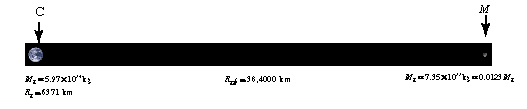
\includegraphics[width=0.9\textwidth]{images/motion-moon.pdf} 
\caption{月球和地球以及月地距离的真实尺寸}
\label{fig: 月球和地球以及月地距离的真实尺寸}
\end{center}
\end{figure}



能否将一个物体当做质点不仅与物体本身的大小有关,还与所研究的具体问题有关。
如果试图描写跳水运动员入水的动作时,他在入水过程中身体姿态至关重要,所以不能够当做质点来看待。
而在描写一个人从北京到上海的整个过程中,我们自然不必在意相对于上千公里的旅程中身体上各个部位之间的微小差别,这时一个人完全有理由当做一个质点。
同样如图\ref{fig: 月球和地球以及月地距离的真实尺寸}所示在研究月球围绕地球的转动时用一个点代表月球的位置相当精确,而在研究嫦娥号在月球上的着陆时月球肯定不能当做质点看待。



当把运动物体抽象为质点以后,它的位置就由这个点的空间位置来代表,这为我们描写运动带来了极大的简化,首先研究质点的运动,当掌握了足够的研究手段以后就有办法来描写真实物体的复杂运动了。
实际上,即使把运动物体简化为一个点它的运动也不是那么容易描写,为此我们将从最简单的运动形式出发,逐渐推广到一般的情况。
在掌握了描写质点或其它物理对象运动的方式以后将进一步研究支配它们运动背后的原因。


\section{最简单的运动:一维运动}




最简单的运动莫过于一个质点始终保持在一条直线上运动,就称它做直线运动。
一个做一维运动物体的位置的描写十分简单,只需要把一根{\heiti 数轴}(number line)放在它运动的直线上,选择任意一点当做数轴的原点,选择任意一个方向当做数轴的正方向,选择一个给定的长度当做计量长度的单位\footnote{物理学中通常选取米或千米来做为长度单位},一个质点的位置就可以用在该数轴上的坐标来唯一决定。
以这种方式选取的数轴称做描写该质点运动的{\heiti 坐标系(coordinate system)},而该质点某一时刻所在位置在坐标系中的读数就叫做它的{\heiti 位置(position)}或{\heiti 坐标}(coordinate)。
对于一维运动的质点,它在坐标系中的坐标通常用$x$来表示,不过这一点不是必须的。


一维运动的描写相对简单,只要知道了每一时刻它所处的位置就完全掌握了该质点的一维运动行为。
假设有一个质点,在时间$t=0\unit{s}$时的坐标为$x_0$,$t=1\unit{s}$时坐标为$x_1$,$t=2\unit{s}$时坐标为$x_2$……
当知道了它在很多时刻的坐标时,就在一定程度上掌握了它的运动行为,运动质点在不同时刻的坐标值知道的越多,我们对它的运动信息就知道地越多。
知道了一些坐标与时间的关系以后可以用很多方法把它的运动表现出来,以一个参加百米赛跑的运动员为例,描写他从起跑到终点的运动的方法有
\begin{description}
\item[叙述]  第1秒跑了1米,第2秒到了4米,第3秒到了9米,第4秒到了16米,第5秒末到了25米,第6秒末到了35米,第7秒末到了45米,第8秒到了55米,第9秒到了65米,第10秒到了75米,11秒85米,12秒100米,结束。
可以看出叙述的方法是能够为我们提供一些信息,但是有些繁琐,也不太直观。
这种描述方法在日常对话中比较常见,但对于科学研究却有些力不从心。
\item[列表] 同样的运动过程如果用一个表来表达,会节约很多空间。
对于同样的运动用列表法由\ref{tab: 不同时刻短跑选手的位置}给出
可以看到列表法会节省很多空间,但也有一些不够直观,无法快速得到运动快慢的信息。
实践上列表法更多地用于实验的数据的记录。
\begin{table}[htbp]
\begin{center}
\begin{tabular}{|c|c c c c c c c c c c c c|}
\hline
时间(s)&1&2&3&4&5&6&7&8&9&10&11&12\\
\hline
位置(m)&1&4&9&16&25&35&45&55&65&75&85&100\\
\hline

\end{tabular}
\caption{不同时刻短跑选手的位置}
\end{center}
\label{tab: 不同时刻短跑选手的位置}
\end{table}



\item[图像]
物理上最直观的描写质点运动的方法是图像法。
此时我们将建立一个坐标系,用横轴代表所经历的时间,纵轴则是已知时刻质点的位置。
对于前面的短跑选手,用图像法可以将他的运动用图\ref{fig: 短跑选手跑动距离和时间的图像}来描写。
从中可以看出,在比赛开始阶段他越跑越快,而随后一段时间里运动速度大致相同,最后在快接近终点的时候又有一个冲刺过程。
很明显可以看出,用图像来描写质点的运动具有最强的直观性。
\begin{figure}[htbp]
\begin{center}
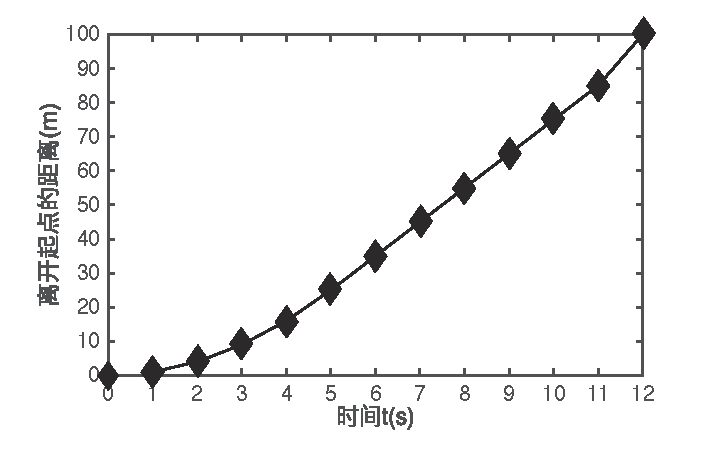
\includegraphics[width=0.5\textwidth]{images/motion-race.pdf}

\caption{短跑选手跑动距离和时间的图像}
\label{fig: 短跑选手跑动距离和时间的图像}
\end{center}
\end{figure}
\end{description}

不难发现以上的三种描写质点运动的方法都无法体现运动的一个最明显的特征:连续性。
运动的质点在每一时刻的位置一般来说都不相同,处于连续的变化过程当中。
为了体现这种特点,我们希望有一种办法对于每一个时刻都能够给出质点的位置,而不是仅仅给出几个特殊时刻的位置。
利用数学中的{\heiti 函数}可以帮助我们得到任意时刻运动质点的位置。
这时一个质点的运动可以表达为
\begin{equation}
x = x(t)
\end{equation}
当函数$x(t)$的形式为已知时,可以得到任意时刻质点所处的位置。
借助函数的图像可以形象地给出质点运动的特征。
例如当一个质点的运动可以用函数$x(t) = 3t$来描写,从中不但可以知道任意时刻质点的位置,还可以从函数的性质得知此时相同的时间里该质点会走过相同的距离。
假如另一个质点的运动函数为$x(t)=5t^2$,同样除了知道任意时刻的位置以及运动的其它性质。



\begin{example}
建立一个竖直向上的坐标系用来表示从它的原点处向上抛出物体的位置。
在不同的时间观察抛体的位置,某次实验得到的结果由下表给出,试着将测量值在坐标系中标出,并试着将其连接为一条光滑的曲线。

\begin{tabular}{|c|ccccccccccccc|}
\hline 
时间 & 0 & 0.5 & 1 & 1.5 & 2 & 2.5 & 3 & 3.5 & 4 & 4.5 & 5 & 5.5 & 6  \\ 
\hline 
位置 & 0 & 8.75 & 15 & 18.75 & 20 & 18.75 & 15 & 8.75 & 0 & -11.25 & -25 & -41.25 & -60 \\ 
\hline 
\end{tabular} 
\begin{center}
\includegraphics[width=0.5\textwidth]{images/motion-problem-empty-coordinate.pdf} 
\end{center}

\end{example}



\begin{example}
已知质点的运动可以用以下函数描写,在坐标系中画出其$x-t$图像。

(1): $x(t) = 5t^2$;(2):$x(t) = \frac{3}{t+1}$;(3):$x(t) = 5\sin(2\pi t)$
\begin{center}
\includegraphics[width=0.9\textwidth]{images/motion-problem-three-empty-coordinate.pdf} 
\end{center}
\end{example}



\begin{example}
已知质点在一条直线上不同时刻的位置随时间的关系由下图给出,指出运动最明显的几个特征。
\begin{center}
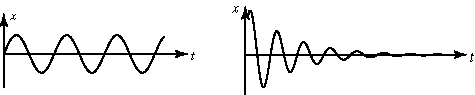
\includegraphics[width=0.8\textwidth]{images/motion-problem-4.pdf}
\end{center}
\tagged{student}{\vspace*{4cm}}
\begin{taggedblock}{teacher}
\noindent
解析:第一个就是简谐振动,第二个是阻尼振动,引导同学从图像中寻找尽可能多的信息。
\end{taggedblock}
\end{example}

事实上不但沿直线运动的质点可以利用以上的方法来描写,只要稍加思索就会发现用同样的方法来描写在弯曲的公路上行驶的汽车也是毫无问题的。
只需要在一条公路上找到一个正方向和原点,而行驶汽车的位置用它在公路上离开原点的距离来标记汽车的位置即可。
我国的公路里程就是用这种方法按照离开北京的距离进行统一标记的。


\subsection{运动的快慢:速率}
虽然当质点坐标随时间的函数为已知时,质点的运动的性质和特点实际上已经完全掌握了,但是我们还是希望从中得到运动有关的更为清楚的信息。
不同的物体运动快慢有着明显的不同,一个正常行走的人比乌龟要快很多,但与路上行驶的汽车比起来很明显要慢,物理上我们定义一个物理量--{\heiti 速率(speed)}来描写这种运动快慢的不同。
其实在过去已经有了一些速率的知识,那时将它称为速度,在物理上要格外注意两者的不同,这里我们谈的是速率,它用来给出运动快慢的量度。
只要想像一下行驶汽车的速率表,就能够马上得到关于速率的一个直观的印象。
过去速率定义为在某一给定的时间$ t$里运动质点所前进的路程,也就是距离$ s$的比值:
\begin{equation}
v = \frac{s}{ t}
\end{equation}
速率的这个定义对于匀速运动的质点来说没有问题,但是对于运动发生变化的过程来说就显得有些粗糙,比如对于静止开始逐渐加速的汽车来说。
很明显在开始的时候速率很慢,随着时间的增加速率则越来越快,为了更准确地描写物体运动的快慢我们需要更精确的速率的定义。
为此我们可以从某一时刻$t$开始计时,通过确定运动质点在某一不长的时间间隔$\Delta t$内前进的距离$\Delta s$与时间间隔$\Delta t$的比值称做在这一小段时间里质点运动的平均速率:
\begin{equation}\label{eqn: motion-平均速率的定义}
\overline{v} = \frac{\Delta s}{\dt}
\end{equation}
可以想像到的是选择越小的$\dt$,以如上方式得到的平均速率对运动质点在时间$t$时运动快慢的描写就越精确。

事实上$\dt$的选取是任意的,不同的$\dt$选取会得到不同的平均速率。
如果一个质点的运动用方程 $x=5t$ 来描写,那么对于任意的$t$,不同的$\dt$选取对平均速率实际上没有影响:
\begin{equation}
\overline{v} = \frac{5(t+\dt)-5t}{\dt} = \frac{5\dt}{\dt} = 5\unit{m/s}
\end{equation}
从运动方程来看我们也很清楚这时质点在做匀速运动,相同的时间里走过相同的距离。
但是如果另一个质点的运动方程为$x=5t^2$时,就不一样了,从函数的图像可以看出随着时间的增加看上去运动速度越来越快。
假如我们想知道在$t=1\unit{s}$时的速率,就需要在$t=1\unit{s}$时选择一个$\dt$并根据定义\ref{eqn: motion-平均速率的定义}来算出对于不同$\dt$时的平均速率。
\begin{eqnarray*}
\dt = 1&,&\overline{v} = \frac{5(1+1)^2-5}{1} = 15\unit{m/s}\\
\dt = 0.1&,&\overline{v} = \frac{5(1+0.1)^2-5}{1} = 10.5\unit{m/s}\\
\dt = 0.01&,&\overline{v} = \frac{5(1+0.01)^2-5}{1} = 10.05\unit{m/s}\\
\dt = 0.001&,&\overline{v} = \frac{5(1+0.001)^2-5}{1} = 10.005\unit{m/s}\\
\dt = 0.0001&,&\overline{v} = \frac{5(1+0.0001)^2-5}{1} = 10.0005\unit{m/s}\\
\dt = 10^{-n}&,&\overline{v} = \frac{5(1+10^{-n})^2-5}{1} = [10+5\pow{-n}]\unit{m/s} 
\end{eqnarray*}
从上面的计算可以很容易地看出,$\dt$取得越小所计算出的平均速率与$10\unit{m/s}$越接近,数学上将$\dt$取得小得不能再小时通过式\ref{eqn: motion-平均速率的定义}算出的运动质点在某一时刻到与它相邻极小时间里的平均速率称做运动质点在该时刻的{\heiti 瞬时速率}
\begin{equation}
v(t) = \lim_{\dt\rightarrow 0}\frac{\Delta s}{\dt}.
\end{equation}
行驶的汽车在每时每刻速率表的读数就是汽车在此时的瞬时速率。

当质点在某一时刻的瞬时速率为已知时,它在随后某一时间间隔$\dt$里所能够前进的距离就是瞬时速率$v$与时间间隔$\dt$的乘积
\begin{equation}\label{eqn: motion-ds=vdt}
\Delta s = v \dt.
\end{equation}
与瞬时速率的情况一样,$\dt$取得越小用这样的方式算出的前进距离与真实的前进距离的差别越小。
还以前面的运动$x(t)=5t^2$为例,已知在$t=1\unit{s}$时的瞬时速率$v = 10\unit{m/s}$,对于不同的$\dt$选取通过两种方法算出的前进距离分别为
\begin{eqnarray*}
\dt = 1,& \overline{v}\dt = 10\unit{m},&x(1+1)-x(1) = 15\unit{m}\\
\dt = 0.1,& \overline{v}\dt = 1\unit{m},&x(1+0.1)-x(1) = 1.05\unit{m}\\
\dt = 0.01,& \overline{v}\dt = 0.1\unit{m},&x(1+0.01)-x(1) = 0.1005\unit{m}\\
\dt = 10^{-n},& \overline{v}\dt = 10^{1-n}\unit{m},&x(1+10^{-n})-x(1) = [10^{1-n}+5\pow{-2n}]\unit{m}\\
\end{eqnarray*}
虽然有一些差别但是随着$\dt$变小,两者之间的差别就越来越小,虽然这种差别永远不会消失,但当$\Delta t\rightarrow 0$时用式\ref{eqn: motion-ds=vdt}来近似地表示质点前进的距离对于计算和分析都非常方便。


\begin{example}
下表为对于给定质点某一运动过程位置随时间关系的测量,求它在相邻两次测量之间运行的平均速率。

\begin{tabular}{|c|ccccccccccccc|}
\hline 
时间 & 0 & 0.5 & 1 & 1.5 & 2 & 2.5 & 3 & 3.5 & 4 & 4.5 & 5 & 5.5 & 6  \\ 
\hline 
位置 & 0 & 8.75 & 15 & 18.75 & 20 & 18.75 & 15 & 8.75 & 0 & -11.25 & -25 & -41.25 & -60 \\ 
\hline 
\end{tabular} 
\tagged{student}{\vspace*{4cm}}
\begin{taggedblock}{teacher}
\noindent
解析:注意这里求的是速率,所以要关注的是在给定时间段内走过的路程。
以1到1.5秒时间段为例,平均速率
\[
\overline{v} = \frac{18.75-15}{0.5} = \frac{3.75}{0.5} = 7.5\unit{m/s}
\]
其它时间段用相同的方法可以得到。
\end{taggedblock}
\end{example}

当在坐标系中谈论质点的运动时要特别注意的一点是,在建立坐标系的过程中我们已经假定了一个正方向,这样沿着坐标轴正方向的运动和沿着坐标轴负方向的运动虽然在相同时间里走过的路程是一样的,但经过一定的时间以后质点所处的位置却不同。
这一点在上面的例子当中也能够看出,从$t=0$到$t=2$的时间里,质点是沿着坐标轴的正方向运动,而在随后的时间里质点的运动方向则是与轴反向。
为了区别这种不同,在给出质点运动速率的同时就必须指出运动的方向,对于沿直线运动着的质点,沿着两个不同方向运动可以通过为速率指定一个正负号的办法达到。
当考虑了质点运动方向以后,速率就有了新的名称--{\heiti 速度(velocity)},对于沿轴运动着的质点,它的运动速度$v$能够为我们提供两个信息:质点本身移动的快慢用速度的绝对值给出,而移动的方向则由速度的正负号决定,当速度取正数时质点沿着轴正方向运动,反之当速度为负时质点则沿着轴的负方向运动。

对于一个以速度$v$匀速运动着的质点来说,如果$t$时刻它位于坐标轴上的$x_0$处,那么在此后的$\Delta t$时间之后,它所处位置的坐标$x$可以表达为
\begin{equation}
x = x_0 +v\Delta t
\end{equation}
无论质点的运动方向如何上式总是成立的。
对于那些不做匀速运动的质点,可以将$v$取做某一时刻的瞬时速度,那么对于越小的$\Delta t $的选取,由上式给出的坐标值就越精确。

\begin{example}
两个在同一直线上以匀速相向运动的质点$A$和$B$,在直线上建立坐标$Ox$,在开始时刻它们分别$x_A = -5\unit{m}$,$x_B=10\unit{m}$的位置。
已知质点$A$向着坐标正方向以$1.5\unit{m/s}$的速率运动,$B$逆着轴向运动,速率为$0.5\unit{m/s}$,求它们相遇的时间和位置。
 \tagged{student}{\vspace*{4cm}}
\begin{taggedblock}{teacher}
\noindent
解析:可能在小学就学过的相遇问题,是一个学习在坐标系中描写运动很好的例子。
两个质点的运动在坐标系中分别为
\[x_A = -5+1.5 t,\qquad x_B = 10-0.5 t\]
它们相遇时要求$x_A = x_B$,联立两个方程可以解出
\[t = 7.5\unit{s},\qquad x = -5+1.5\times 7.5 = 6.25\unit{m}\]
\end{taggedblock}
\end{example}

\subsection{图像详解}
\begin{figure}[htbp]
\begin{center}
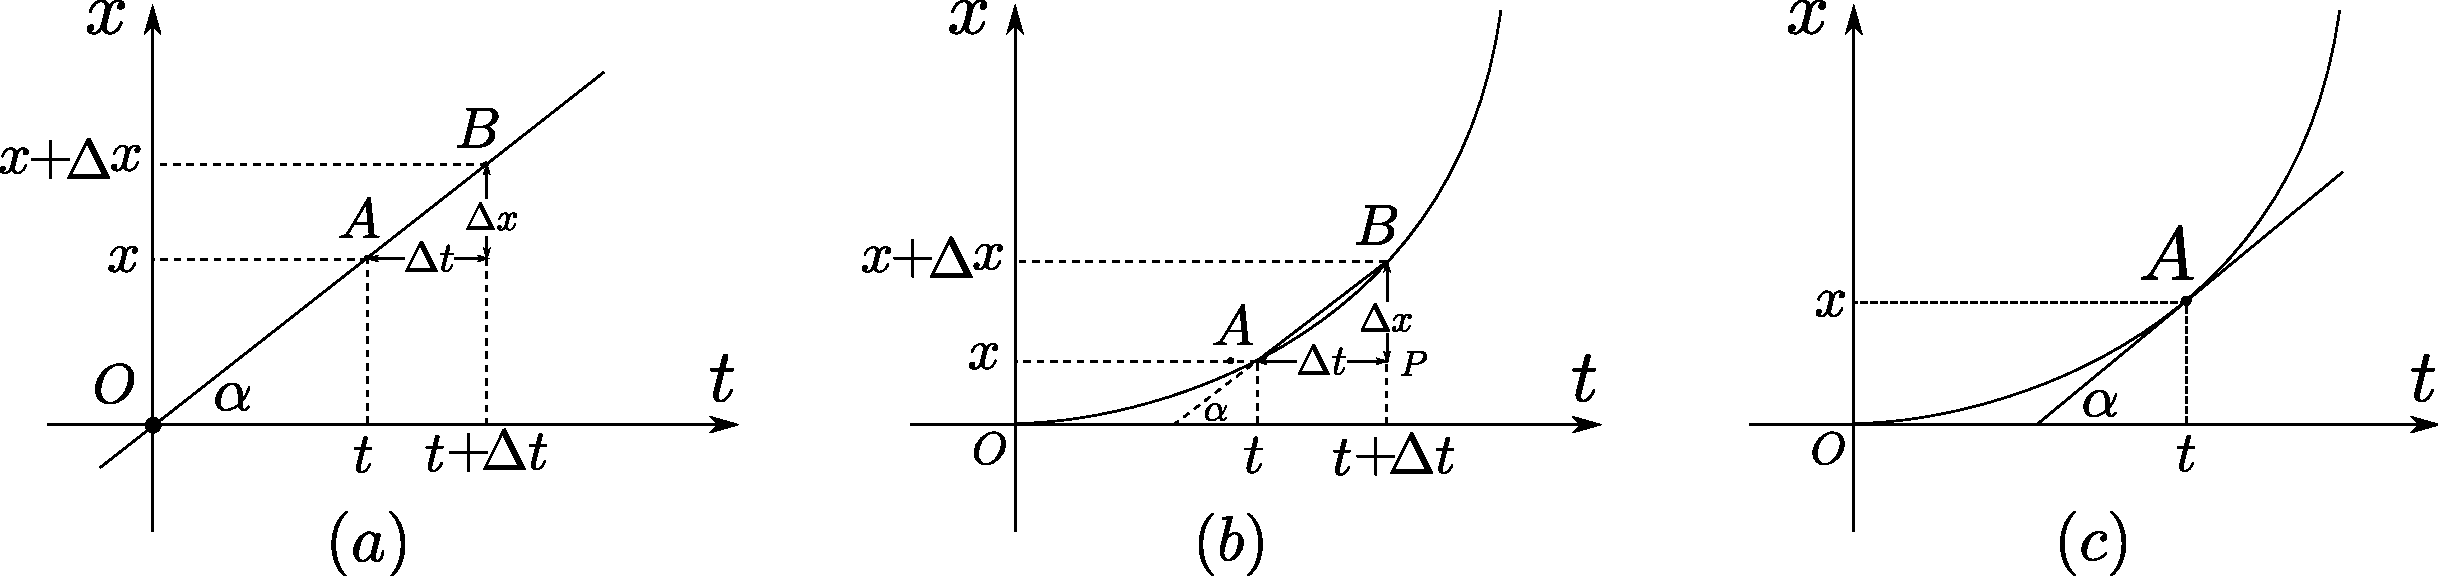
\includegraphics[width=0.8\textwidth]{images/motion-x-t.pdf}
\caption{一维运动$x-t$图像以及平均速率和瞬时速率的几何意义。(a)对于匀速直线运动来说,它的图像是一条直线,任意时刻的速率均为表示运动的直线的斜率。(b)一般运动过程中从$t$到$t+\Delta t$时间间隔中的平均速率,它是连接曲线上两点$A、B$构成的直线的斜率,直线上A、B两点之间的部分有时被称为曲线的割线。(c)当$\Delta t\rightarrow 0$时,B点和A点无限地接近,在图中已经无法区分两个点,这时用来衡量两个时间点里距离变化的割线也变成了曲线的切线,而切线的斜率正是运动物体在$t$时刻的瞬时速率。}
\label{fig: motion一维运动$x-t$图像以及平均速率的几何意义}
\end{center}
\end{figure}
无论是坐标,还是速度当质点运动时都能够用时间的某种函数来给出。
既然是函数,我们就可以将它们在坐标系中画出来,这样就可以很形象地看出运动函数所具有的性质,并且还能够得到不同物理量之间的联系。


最简单的图像自然就是坐标与时间的图像,有时称之为$x-t$图像,如图\ref{fig: motion一维运动$x-t$图像以及平均速率的几何意义}所示。
从图中可以很容易地找出某一给定时刻质点的坐标。
如果一个质点以匀速运动,那么它的$x-t$图像用图\ref{fig: motion一维运动$x-t$图像以及平均速率的几何意义}(a)中的直线表示,并且可以从图中看出质点运动的速率就是这条直线与横轴夹角$\alpha$的正切。

另外从$x-t$图像中其实我们还能够得到质点在某一时间段的平均速度,假设某一$t$时刻质点的坐标为$x$,它可以用图中的A点代表。
同理在时刻$t$之后一某个时间间隔$\dt$后它的坐标变成了$x+\Delta x$,可以用图中的B点来代表。
这样在$\dt$时间里的平均速率
\begin{equation}
\overline{v} = \frac{\Delta x}{\dt}
\end{equation}
就是图中直角三角形APB当中角$\alpha = \angle PAB$的正切。
对于越来越小的时间间隔$\dt$的选取,B点与A点的距离会越来越近,与此同时割线AB与曲线在A点的切线,就是那条与A点仅有一个交点的线产差别越来越小。
最终当B点无限地接近于A点时,割线AB就变成了曲线在A点的切线,而此时切线与横轴夹角的正切,也就是切线的斜率就是运动质点在此时的瞬时速率。






\begin{example}
根据如下x-t图像判断速度的变化趋势
\begin{center}
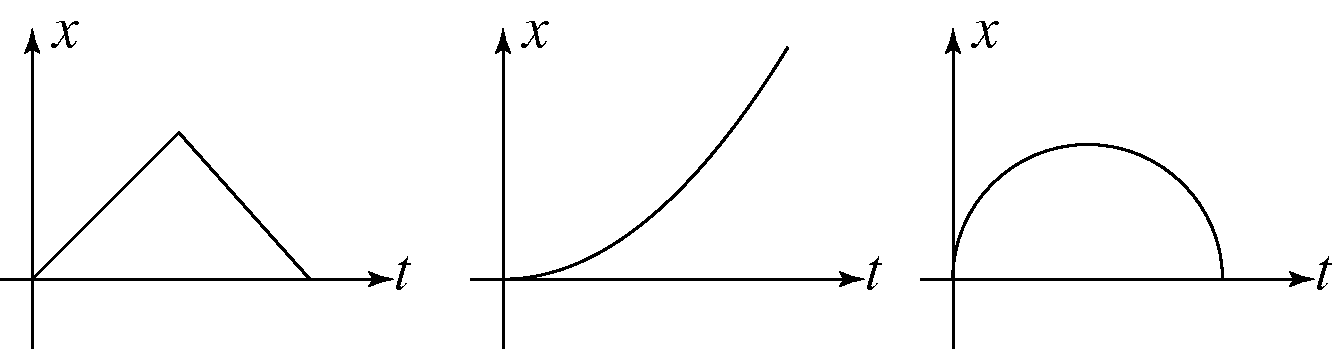
\includegraphics[width = 0.9\textwidth]{images/motion-problem-5.pdf}
\end{center}
\tagged{student}{\vspace*{3cm}}
\begin{taggedblock}{teacher}
\noindent
解析:根据图像分析即可,尽可能多提取出运动的信息。
\end{taggedblock}
\end{example}





\begin{figure}[h]
\begin{center}
\includegraphics[width=0.8\textwidth]{images/motion-v-t.pdf}
\caption{一维运动$v-t$图像和运动距离的几何意义}
\label{fig: motion一维运动$v-t$图像以及运动距离的几何意义}
\end{center}
\end{figure}

除了$x-t$图像以外我们还可以做出$v-t$图像,也就是将不同时刻的速度用坐标系中的曲线连接起来,可以想像成在行驶的汽车里根据不同时刻速率表的读数。
当一个物体的运动速率不变时,它的$v-t$图像为一条平行一时间轴的一条直线,很明显一段时间里匀速运动质点前进的距离为速率与时间的乘积,图\ref{fig: motion一维运动$v-t$图像以及运动距离的几何意义}(a)当中矩形ABDC的面积就是由A到B点所代表的时间里质点前进距离。
当物体速率并不是常数而是随时间而变时,它的$v-t$图像如图\ref{fig: motion一维运动$v-t$图像以及运动距离的几何意义}(b)所示,其中轴坐标为对应时刻的瞬时速率。
根据\ref{eqn: motion-ds=vdt}式,质点在某一点处瞬时速率与之后一段微小时间间隔的乘积随着$\dt$取得越小则与真实运动在相同时间里所前进的距离越接近。
这样当给出$v-t$图像之后,物体前进的距离可以用图\ref{fig: motion一维运动$v-t$图像以及运动距离的几何意义}(b)当中很多宽为小的时间间隔,高为对应时刻的瞬时速度构成的窄矩形的面积的和。
可以看出,这些窄矩形的面积和在$\dt$越来越小时与图\ref{fig: motion一维运动$v-t$图像以及运动距离的几何意义}(c)当中由ABDC四个点围成区域的面积越来越接近!
也就是说,当给出$v-t$图像以后一段时间里质点前进的距离为$v-t$图像在两个时间点之间与横轴包围的曲线的面积。



\begin{example}
若质点作直线运动的速度$v$随时间$t$变化的图像如下图所示,则该质点的位移$x$(从$t=0$开始)随时间$t$变化的图像可能是下面的哪一个?
\begin{center}
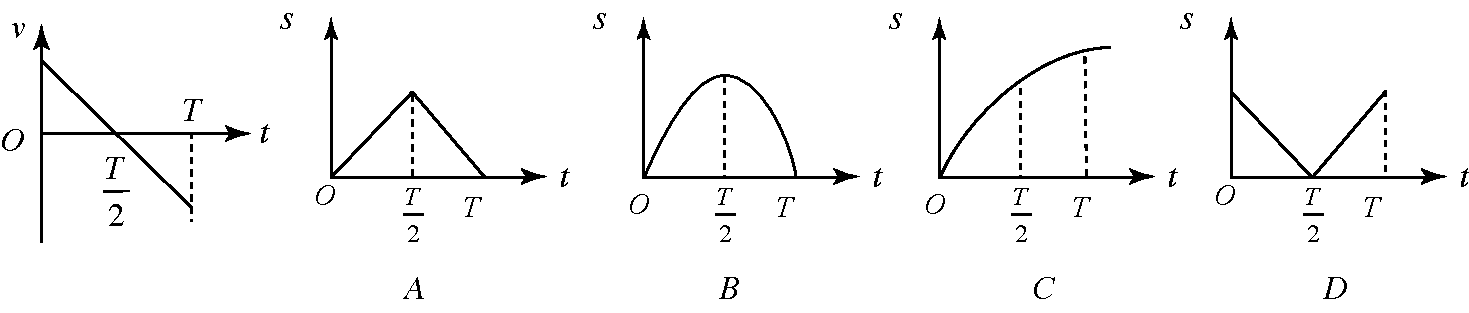
\includegraphics[width=0.9\textwidth]{images/motion-problem-39.pdf}

\end{center}
\tagged{student}{\vspace*{1cm}}
\begin{taggedblock}{teacher}
\noindent
解析:位移先变大后变小,开始时刻位移为零,根据图像可知最终位移也是零,所以答案是$B$。
\end{taggedblock}
\end{example}

\begin{example}
求质点在用以下 $v-t$图所表示的运动过程当中从初始时刻$t=0$出发到图中给定的$t$时刻当中所走过的总路程。
\begin{center}
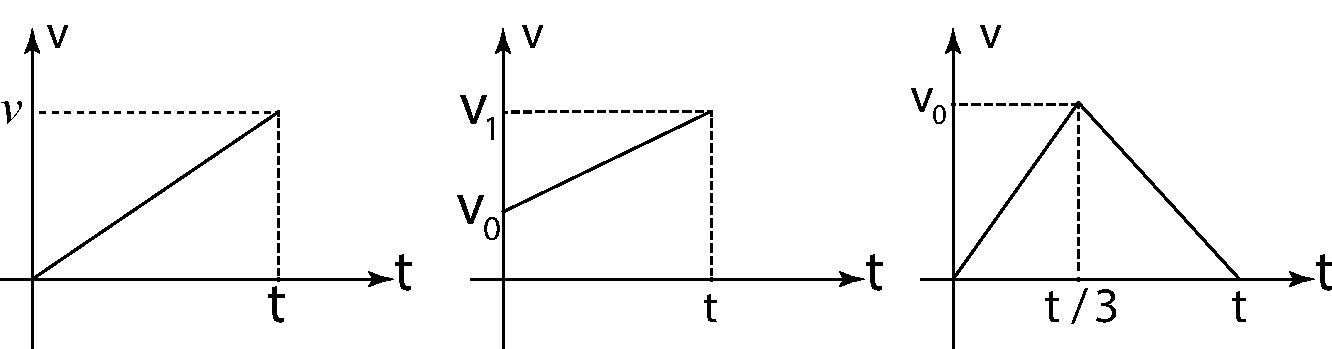
\includegraphics[width = 0.9\textwidth]{images/motion-problem-6.pdf}
\end{center}

\tagged{student}{\vspace*{4cm}}
\begin{taggedblock}{teacher}
\noindent
解析:所有的运动速度方向不变,所以$v-t$图像与$x$轴围成的面积就是走过的路程,这样
\begin{eqnarray*}
S_1 &=& \frac{1}{2}vt\\
S_2 &=& \frac{1}{2}(v_0+v_1)t\\
S_3&=& \frac{1}{2}v_0t
\end{eqnarray*}

\end{taggedblock}
\end{example}




\subsection{加速度,匀加速运动}
一般来说一个质点的运动速率总是在不断地发生变化,只要想像一辆行驶在路上的汽车就能够得到这样的印象。
正是因为这一点引入一个物理量来描写速率变化的快慢是很有必要的。
假设一个质点在某一时刻$t$的速率为$v(t)$,而在此后的$\dt$间隔之后由于某种原因变成了$v(t+\dt)$,在这个运动过程中速率的增加量自然就是$\Delta v = v(t+\dt)-v(t)$,那么加速度就被定义为速率的变化量与发生这一速率变化所需要时间$\dt$的比值:
\begin{equation}\label{eqn: motion-加速度的定义}
a = \frac{\Delta v}{\dt} = \frac{ v(t+\dt)-v(t)}{\dt}.
\end{equation}
很明显,如果在给定时间里速率变化量越大就对应着较大的加速度,反之若在相同的时间里速率只发生了很小的改变,那么意味着较小的加速度。
物理上用{\heiti 加速度(acceleration)}来衡量速度变化的快慢和方式。
如果上式中的间隔$\dt$是一个相对较大的时间,在该时间前后速度发生了相当可观的变化,那么由上式定义出的加速度就是$\dt$时间里的{\heiti 平均加速度}。
而当$\dt$取得非常之小,就可以认为由上式得到的实际上是运动质点在$t$时刻的{\heiti 瞬时加速度}。

当在一段时间里质点运动的加速度保持不变,这样的运动就被称为{\heiti 匀加速运动}。
若加速度为$a$且不随时间而变,在$t=0$的时刻质点的初始速率为$v_0$,那么在此之后的任意时刻$t$质点运动的速率则是
\begin{equation}\label{eqn: motion-v=v0+at}
v(t)=v_0+at.
\end{equation}
可以看出速度随时间线性增加,此时的$v-t$图像由图所示。
我们知道$v-t$图像在给定的两个时间点下包围的面积就是在该时间间隔当中质点的路程,当质点初始坐标为$x_0$时此后任意$t$时间它的坐标则是
\begin{equation}\label{eqn: motion=x=x0+v_0t+1/2at^2}
x(t)=x_0+v_0t+\frac{1}{2}at^2.
\end{equation}

和速度一样,加速度也可用它与时间的图像来形象地给出,匀加速度运动质点的$v-t$图像是一条直线,根据前面的经验可知加速度对应于该直线与时间轴夹角的正切,也就是该直线的斜率。
对于一般的情况,在任意时刻$t$加速度则是$v-t$曲线在该点处切线的斜率。
反过来当给出$a-t$图像时,两个给定时间之间$a-t$曲线下的面积则对应于这一段时间里速度的变化量。


\begin{example}
根据速度-时间图像由\ref{eqn: motion-v=v0+at}推出匀加速运动中位置随时间的变化关系式\ref{eqn: motion=x=x0+v_0t+1/2at^2}。
\tagged{student}{\vspace*{4cm}}
\begin{taggedblock}{teacher}
\newline
解析:匀加速度运动的$v-t$图像是直线,所以位移就是直线与横轴围成的面积,这样我们就有
\[
x(t)-x_0 = \frac{1}{2}(v_0+v_0+at)t = v_0t+\frac{1}{2}at^2,
\]
移项就可得证。
\end{taggedblock}
\end{example}

\begin{example}
加速度$a$作匀加速运动的质点初速度$v_1$,位置为$x_1$,在经过一段时间以后它的速度变成了$v_2$,运动到了坐标轴上的$x_2$处,证明以上物理量之间满足关系式
\[
v_2^2-v_1^2=2a(x_2-x_1)
\]
\tagged{student}{\vspace*{4cm}}
\begin{taggedblock}{teacher}
\noindent
解析:匀加速运动过程速度、位置随时间的变化规律分别为
\[v_2=v_1+at,\qquad x_2=x_1+v_1 t+\frac{1}{2}at^2\]
由第一个式子解出时间$t$得到
\[
t = \frac{v_2-v_1}{a}
\]
代入第二个式子就可以从两个方程当中消去时间,得到位置、速度和加速度之间的关系
\[
x_2-x_1 = v_1\frac{v_2-v_1}{a}+\frac{1}{2}a\frac{(v_2-v_1)^2}{a}
\]
将上式化简之后就可证明上述关系。
\end{taggedblock}
\end{example}

%%%%%%%%%%%%%%%%%%%%%%%%%%%%%%%%%%
\begin{example}
一列火车以给定的加速度沿直线轨道前进。
当列车前端通过点$O$时,列车的速度为$u_1$,当列车尾端通过$O$点时,速度为$u_2$,试求列车中部通过$O$点时的速度$v$。
\tagged{student}{\vspace*{4cm}}
\begin{taggedblock}{teacher}
\newline
解析:设列车长度为$L$,加速度为$a$,根据前面的公式我们有
\[
u_2^2-u_1^2 = 2aL,
\]
当中点通过时走过的路程是列车总长的一半,所以
\[
v^2-u_1^2 = 2a\frac{1}{2}L = aL = \frac{u_2^2-u_1^2}{2},
\]
整理之后可得
\[
v^2 = \frac{1}{2}(u_1^2+u_2^2),\qquad v = \sqrt{\frac{1}{2}(u_1^2+u_2^2)}.
\]
\end{taggedblock}
\end{example}
%%%%%%%%%%%%%%%%%%%%%%%%%%


\begin{example}
一辆汽车在公路上以速度$v_0 = 20\unit{m/s}$沿直线行驶,当它到达路口前$60\unit{m}$处发现交通信号的倒计时还剩$2\unit{s}$,如果他想加速通过路口,所需的加速度至少为多少?
如果他不想闯红灯,停止所需要的加速度至少为多少?
\tagged{student}{\vspace*{4cm}}
\begin{taggedblock}{teacher}
\newline
解析:若想通过路口,必须在2s内走完剩下的60m,设加速度为$a_1$,如果刚好通过,需要有
\[
v_0 t +\frac{1}{2}a_1t^2 = 60,\qquad a>a_1 = 10\unit{m/s^2}
\]
反之要想停下来,根据实际情况,对运动的时间没有要求,而是要在60m内停下来,设刚好停下来的加速度为$a_2$
\[
0-v_0^2 = 2a_2L,\qquad a<a_2 \simeq -3.3\unit{m/s^2}
\]
\end{taggedblock}
\end{example}

\begin{example}
A火车以$v_1=20\unit{m/s}$的速度匀速行驶,司机发现前方同轨道上相距$100\unit{m}$处有另一列火车正以$v_2=10\unit{m/s}$的速度匀速行驶,$A$车立即做加速度大小为$a$的紧急制动。
求能够使两车不至于相撞的$a$的最小取值。
\tagged{student}{\vspace*{4cm}}
\begin{taggedblock}{teacher}
\newline
解析:建立以火车$A$发现前车时刻$A$的位置为原点的坐标系,设$A$的加速度为$a$,两车的运动方程分别为
\[
x_A = v_1t+\frac{1}{2}at^2,\qquad x_B = 100+v_2t,
\]
如果两车不会相撞,那么意味着方程$x_A = x_B$无解:
\[
\frac{1}{2}at^t+(v_1-v^2)t-100 = 0,\qquad \frac{1}{2}at^t+10t-100 = 0
\]
二次方程无解要求判别式小于零:
\[
\Delta  = 100+200a<0,\qquad a<0.5\unit{m/s^2}
\]
\end{taggedblock}
\end{example}




\begin{example}
在通过某一弯道之后的大直道上两辆赛车展开追逐,后车的速度为$v_1$,前车的速度$v_2>v_1$,后车具有更好的加速性能$a_1>a_2$,两车相距$d$且直道的全长为$L$。
简单起见将两辆车都看成质点,求后车能够在直道上超越前车的条件。
\tagged{student}{\vspace*{4cm}}
\begin{taggedblock}{teacher}
\newline
解析:以后车的位置为原点建立坐标系,这样两车的运动可写为
\[
x_1 = v_1t+\frac{1}{2}a_1t^2,\qquad x_2 = d+v_2t+\frac{1}{2}a_2t^2
\]
不考虑赛道长度的情况下一定可以追上,追上的时间由方程$x_1=x_2$给出,它的解为
\[
t = \frac{(v_2-v_1+\sqrt{(v_2-v_1)^2+2(a_2-a_1)d})}{a_1-a_2},
\]
如果考虑了赛道的长度,就要求在上式解的时刻后面赛车走过的路程小于总长:
\[
v_1t+\frac{1}{2}a_1t^2<L,
\]
这样就可以给出能够追上所满足的条件。
\end{taggedblock}
\end{example}





\subsection{落体运动}
将一个重物由静止释放以后的运动就是一种均加速运动,以这种方式运动的物体称为{\heiti 自由落体}。
为了和今后的表达方式一致,建立一个竖直向上的坐标系$x$,物体由坐标系的原点处静止释放,实验表明任何自由落体都以相同的加速度均加速下落,加速度指向地面,随着时间的推移其速率均匀增加
\begin{equation}
v(t) = -gt,
\end{equation}
位置随时间的关系则是
\begin{equation}
x(t) = -\frac{1}{2}gt^2,
\end{equation}
其中$g\simeq 9.8 \unit{m/s^2}$,称为地球表面的{\heiti 重力加速度}。


当初始时刻$t=0$时速度或坐标取非零值时自由下落物体速度和位置随时间的变化关系由一般情况下的均加速运动满足的规律给出。
如果$t=0$时自由落体的位置和速度分别为$x_0$和$v_0$时,此后它的速度和位置随时间的关系为
\begin{equation}
v(t) = v_0-gt,\qquad x(t) = x_0+v_0t-\frac{1}{2}gt^2.
\end{equation}

\begin{example}
将竖直向上的坐标轴原点取成抛出物体的那一点,在以下各种情况下求质点的坐标:

(1)由静止开始下落的质点$1\unit{s}$、$5\unit{s}$、$10\unit{s}$时。

(2)向上以初速度$v_0=10\unit{m/s}$抛出质点在$1\unit{s}$、$2\unit{s}$、$3\unit{s}$时。

(3)向下以初速度$v_0=10\unit{m/s}$抛出质点在$1\unit{s}$、$2\unit{s}$、$3\unit{s}$时。
\tagged{student}{\vspace*{4cm}}
\begin{taggedblock}{teacher}
\newline
解析:三种情况下的运动方程分别为
\[
x_1 = -\frac{1}{2}gt^2,\qquad x_2 = 10t-\frac{1}{2}gt^2,\qquad x_3 = -10t-\frac{1}{2}gt^2,
\]
将各个时刻代入即可。
\end{taggedblock}
\end{example}

\begin{example}
建立竖直向上的坐标系$x$,从原点出发以初速度$v_0 = 20\unit{m/s}$竖直上抛的一个质点,质点的$x$坐标值就相当于抛出以后运行的高度。
求它运动到高度分别为 15 m、20 m 、25 m 、0 m 、-25m处所需要的时间。
为简单起见设$g=10 \unit{m/s^2}$
\tagged{student}{\vspace*{4cm}}
\begin{taggedblock}{teacher}
\newline
解析:设希望知道时间的高度为$h$,那么到达该高度的时间由方程
\[
h = 20t-5t^2,\qquad  5t^2-20t+h = 0
\]
给出,将各个高度代入上式求解二次方程即可得到时间:
\begin{enumerate}
\item x=15 m: 方程$5t^2-20t+15=0$,有两个解$t=1s,3s$,分别对应于上升阶段和下降阶段到达该高度的时间。
\item x=20 m: 方程$5t^2-20t+20=0$, 只有一个解$t=2s$,意味着到达最高点。

\item  x=25 m: 方程$5t^2-20t+25=0$,判别式小于零,无解,意味着给定的初速度飞不了这么高。

\item x=0m: 方程$5t^2-20t=0$, 两个解$t=0,4$,一个解对应于扔出的时刻,一个解对应于再次落回来的时刻。

\item x=-25m: 方程$5t^2-20t-25=0$,两个解$t=5,-1$,一个解正是落回来的时刻,另一个解对应于过去的时间,意味着一个在更低的点抛出物体,它正好在$t=0$的时刻通过这里的坐标原点且速度刚好是向上$20\unit{m/s}$的物体,它在上升过程中到达原点下方$25\unit{m}$处的时间,自然它对应于$t<0$的时间。
\end{enumerate}
\end{taggedblock}
\end{example}

\begin{example}
如图所示在地面上方高度为$h$处有一个质点$A$自由下落的同时从地面以初速度$v_0$竖直上抛另一个质点$B$,求它们能够在空中相遇的最小上抛速度$v_0$。
\begin{flushright}
\includegraphics[width = 0.2\textwidth]{images/motion-one-up-one-down.pdf} 
\end{flushright}
\tagged{student}{\vspace*{1cm}}
\begin{taggedblock}{teacher}
\noindent
解析:建立一个原点在地面竖直向上的坐标系$Ox$,两个质点的运动方程分别为
\[x_A= h-\frac{1}{2}gt^2,\qquad x_B = v_0 t-\frac{1}{2}gt^2\]
设它们将于时刻$t$相遇,$t$满足方程
\[x_A = x_B,\qquad h = v_0 t,\qquad t=\frac{h}{v_0}\]
这么长的时间里$A$下落的高度必须小于$h$,这样它们才能够在空中相遇:
\[
\frac{1}{2}gt^2=\frac{1}{2}g(\frac{h}{v_0})^2\le h
\]
很容易解出$v_0$必需满足条件
\[ v_0^2\le \frac{1}{2}gh\]
\end{taggedblock}
\end{example}

\begin{example}
一个女子从高楼上落下,超人于时间$T$之后发现了这件事,超人立即以初速度$v_0$加速向下飞去救该女子。
假设女子下落和超人的飞行作自由落体运动,假设楼高$H$,求超人能够在女子落地前将她救起的最小初速度$v_0$。

\tagged{student}{\vspace*{4cm}}
\begin{taggedblock}{teacher}
\noindent
解析:选择超人发现以后的时刻为计时的起点,坐标系从楼顶算起竖直向下,开始时刻女子的速度$gT$,位置$\frac{1}{2}gT^2$,两者的运动方程分别为
\[
x_S = v_0t+\frac{1}{2}gt^2,\qquad x_g = \frac{1}{2}gT^2+gTt+\frac{1}{2}gt^2
\]
两人能够在空中相遇需要他们的坐标一致并且超人走过的距离比楼高要小。
简单的计算表明他们相遇的时间
\[
t = \frac{\frac{1}{2}gT^2}{v_0-gT},
\]
可见如果$v_0<gT$则无论如何也追不上,反之如果能够追上,那么追上时超人下降的高度
\[
h = v_0t+\frac{1}{2}gT^2 = \frac{1}{2}gT^2\frac{v_0^2-gTv_0-\frac{1}{4}g^2T^2}{(v_0-gT)^2} = \frac{1}{2}gT^2\frac{(v_0-\frac{1}{2}gT)^2}{(v_0-gT)^2}<H,
\]
经过计算可解出
\[
v_0>gT\frac{\sqrt{\frac{2H}{gT^2}}-\frac{1}{2}}{\sqrt{\frac{2H}{gT^2}}-1}
\]
\end{taggedblock}
\end{example}

\begin{example}
一质点自距离水平地面高$H$处自由下落,每次与地面发生碰撞以后反弹的速率均为撞向地面速率的$e$倍,$e<1$。
求自第一次反弹以后算起到最终停止所需要的总时间和质点走过的总路程。
\begin{flushright}
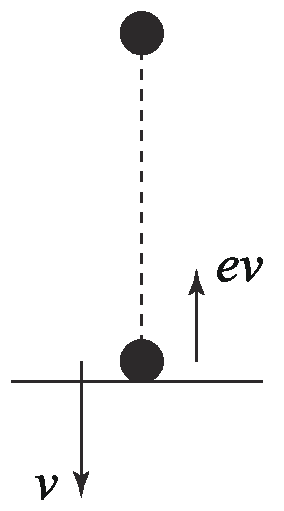
\includegraphics[width = 0.2\textwidth]{images/motion-29.pdf} 
\end{flushright}
\tagged{student}{\vspace*{0cm}}
\begin{taggedblock}{teacher}
\noindent
解析:第一次反弹之前质点撞向地面的速率$v_0 = \sqrt{2gH}$。
第一次反弹之后其向上的速率变成$v_1=ev_0$,上升到下落所需要的总时间$t_1 = \frac{2v_1}{g} = 2e\frac{v_0}{g}$,到第二次撞向地面之前走过的总路程$s_1 = e^2\frac{v_0^2}{g} = e^2H$。
很容易将这些结论推广到随后的情况,这样到最终停止时所经历的总时间
\[ T = \sum_{n=1}^\infty t_n =  \frac{2v_0}{g}\sum_{n=1}^\infty e^n = \frac{2v_0}{g} \frac{e}{1-e}  = 2 \sqrt{ \frac{2H}{g}} \frac{e}{1-e},\]
同样的道理到最终停止所走过的总路程则是
\[  S = \sum_{n=1}^\infty s_n =  H \sum_{n=1}^\infty e^{2n} = H\frac{e^2}{1-e^2}.\]
它们都是有限的,这一点从直观上不太容易发现。
\end{taggedblock}
\end{example}


%%%%%%%%%%%%%%%%%%%%%%%%%%%%%%%%%%
\begin{example}
一个质点以初速度$v_0$撞向一个板,第一次与板碰撞反弹以后的运动变成加速度指向板的匀加速运动,加速度大小为$a$,此后每次与板碰撞以后速度反向且大小不变,但指向板的加速度变成原来的$k(k>1)$倍。
求此后运动的总时间和质点走过的总路程。
\tagged{student}{\vspace*{4cm}}
\begin{taggedblock}{teacher}
\newline
解析:和前一问一样的思路,第一次反弹以后的运动记做第0次运动,这样就有递推关系:
\[  a_n = k^na,\qquad t_n = \frac{1}{k^n}\frac{2v_0}{a},\qquad s_n = \frac{1}{k^n}\frac{v_0^2}{a},\]
这样总时间和总路程为
\[
T = \sum_{n=0}^\infty t_n = \frac{2v_0}{a}\frac{k}{k-1},\qquad S = \sum_{n=0}^\infty s_n = \frac{v_0^2}{a}\frac{k}{k-1}.
\]
\end{taggedblock}
\end{example}
%%%%%%%%%%%%%%%%%%%%%%%%%%%%%%%%%%

\begin{example}
有一竖直放置、两端封闭的长玻璃管,管内为真空,管内有一小球自某处自由下落(初速度为零),落到玻璃管底部时与底部发生弹性碰撞,反弹速度与入射速度相同。
以后小球将在玻璃管内不停地上下跳动。
现在支架固定一照相机,用以拍摄小球在空间的位置。
每隔一相等的确定的时间间隔$T$拍摄一张照片,照相机的曝光时间极短,可忽略不计。
从所拍到的照片发现,每张照片上小球都处于同一位置。
求小球开始下落处离玻璃管底部距离(用$H$表示)的可能值以及与各$H$值相应的照片中小球位置离玻璃管底部距离的可能值。
\tagged{student}{\vspace*{6cm}}
\begin{taggedblock}{teacher}
\newline
解析:全国中学生物理竞赛复赛
\end{taggedblock}
\end{example}



\section{高维运动,位移,速度}
前面我们研究的都是做一维运动的质点,定义了位置(坐标),速度和加速度等能够方便描写质点运动的物理量。
当质点的运动并不局限于一条直线或给定的轨道上时,描写它的运动通常要更复杂一些,需要一些新的概念和物理量才能做到。
大多数情况下,尽管质点的运动不在一条直线上,但依然保持在某一个给定的平面中,例如抛体的运动以及地球围绕太阳的公转都满足这一特征,所以我们首先来看一下在一个平面中的运动,当搞明白平面内的运动以后很容易向三维空间运动做推广。
\subsection{位置的确定:坐标系}
在一个平面上确定一个点的位置比在直线上需要更多的信息。
生活上有两种常用的方法来说明两点之间的位置关系,例如说清华大学在从天安门出发向西走6公里再向北走11公里;或者说北京大学在天安门北偏西大约40$^\circ$方向12公里处。
这两种描述方法对应于物理中的两种常用的方式来确定平面上一个点的位置。
\begin{enumerate}
\item 直角坐标系:  如图\ref{fig: motion-两种坐标系}(a)所示,从一个给定点$O$出发沿着两个相互垂直的方向做两个数轴$x,y$,那么任意点的位置可以用它在这两个轴上的投影的坐标值$(x,y)$唯一确定。
当一个点的$x$坐标取负值时说明它在$O$点的左侧,同理当它的$y$坐标值为负数时说明它在$O$点的下方,$x、y$坐标可能的取值范围都是全部的实数值。
\item 平面极坐标系:如图\ref{fig: motion-两种坐标系}(b)所示的从一个给定点$O$出发确定一个给定的方向$ON$,任何一点P的位置用它和$O$点的直线距离$r$以及和给定方向之间的夹角$\theta$来唯一确定。
与直角坐标系不同的是$r$的取值范围是从0开始的正数,$r=0$意味着该点位于图中的$O$点处;角度变量$\theta$的取值有一定的任意性,从角度的一般定义可以看出,对于相同的$r$,当两个角度$\theta_1$和$\theta_2$相差$2\pi$的整数倍时实际上对应于图中的同一个点,在使用的时候要注意这一点。
另外原点$O$处的角度取值并没有实际意义,都对应于图中的$O$点。
\end{enumerate}




\begin{figure}[hbtp]
\centering
\includegraphics[width=0.6\textwidth]{images/motion-theory-1.pdf}
\caption{(a)平面直角坐标系, (b)平面极坐标系}\label{fig: motion-两种坐标系}
\end{figure}

无论选取哪种坐标系来描写质点的运动,都必须在开始描写物理问题之前明确地指出坐标系的取法。
对于直角坐标系来说需要指出原点的位置以及两个轴的正方向分别指向何处;当使用平面极坐标系时需要 指定原点的位置和参考方向的取向,只有当坐标系被明确地给出以后利用坐标系来描写质点的运动才是有意义的。
两种坐标系都可用来唯一地给出质点的位置,在处理不同问题时选择合适的坐标系会使问题极大地简化。
一般来说研究地球上质点的运动时选用直角坐标系来描写质点的位置,但是如果运动有一个明显的中心,例如太阳系中各个行星围绕太阳的转动时用极坐标则会更方便一些。

\begin{example}
在下图所示的平面直角坐标系中标出由以下几个已知坐标的点:

$A:  (3,4); B: (5,0); C: (-3,2);  D: (2,-5); E: (-3,-2); F: (0, 3); G: (-1,0); H: (0,-3) $
\begin{center}
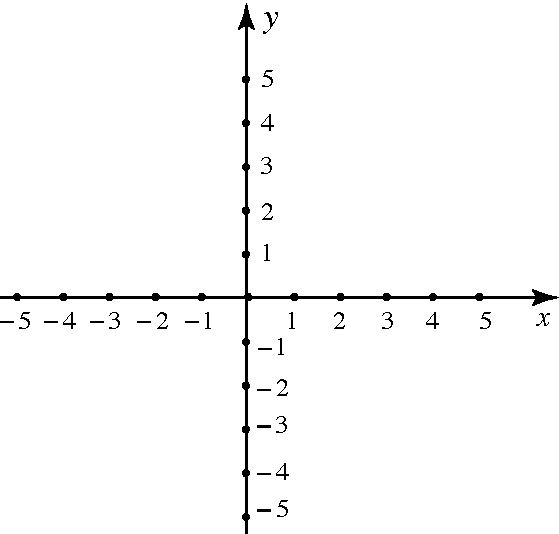
\includegraphics[width=0.4\textwidth]{images/motion-problem-7.pdf}
\end{center}

\tagged{student}{\vspace*{0cm}}
\begin{taggedblock}{teacher}


\end{taggedblock}
\end{example}

\begin{example}
在下图所示的平面极坐标系中标出由以下几个已知坐标的点:

$A: (5, \pi/3); B: (2, \pi/3);  C:(5, \pi/2); D:(4, \pi); E: (4, 3\pi/2)), F: (3,0)$
\begin{center}
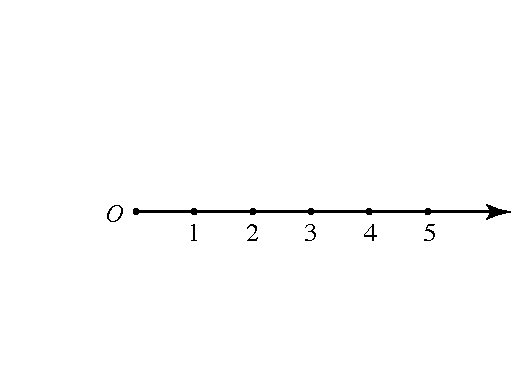
\includegraphics[width=0.4\textwidth]{images/motion-problem-8.pdf}
\end{center}
\tagged{student}{\vspace*{0cm}}
\begin{taggedblock}{teacher}


\end{taggedblock}
\end{example}

\subsection{位置的变化:位移}
当质点在平面上运动,也就是它的位置发生变化时,描述这种变化一般我们会说“它从某处(起点)出发沿着某种路线(轨迹)最后到达了某处(终点)”。
如图\ref{fig: motion-始末点相同但沿着不同路径的运动}所示对于相同的起点$A$和终点$B$会有无数种运动的轨迹(path),沿着不同轨迹的运动很不一样,但它们都有共同的起点和终点。
物理上我们用{\heiti 位移(displacement)}来描写运动质点的位置变化,它的定义很简单,就是一条由起点到终点的一个箭头,即有向线段来给出质点的位移。
这个有向线段的长度代表了位置变化的距离,而它的方向自然给出了位置变化的方向。
这样当初始位置为已知,并且经过某种运动之后的位移也为已知时,在运动结束以后的位置就被唯一确定了。
图\ref{fig: motion-点出发沿给定路径运动到不同位置时质点的位移}给出了从A点出沿着曲线运动的质点在各个不同位置时的位移。
从中可以看出,如果两点非常接近时,位移的大小和质点真正走过的距离非常接近,但当质点沿着轨迹前进一段距离之后位移的大小和所走过路程之间有了明显的差别,并且位移的大小和所走过路程的长短也没有必然的关系。


\begin{figure}[hbtp]
\begin{minipage}[c]{0.45\textwidth}
\includegraphics[height=1in]{images/motion-theory-2.pdf}
\caption{始末点相同但沿着不同路径的运动}
\label{fig: motion-始末点相同但沿着不同路径的运动}
\end{minipage}
\begin{minipage}[c]{0.45\textwidth}
\includegraphics[height=1in]{images/motion-theory-3.pdf}
\caption{从$A$点出发沿给定路径运动到不同位置时质点的位移}
\label{fig: motion-点出发沿给定路径运动到不同位置时质点的位移}
\end{minipage}
\end{figure}

除了用箭头来表示位移,其实我们还可以用一段运动过程前后质点在给定坐标系中坐标值的变化来表示给定过程中的位移。
对于一个在给定平面内运动的质点,建立一个平面直角坐标系$Oxy$,当它在运动开始时刻位于由坐标$(x_1,y_1)$所给出的位置,而在运动结束时的位置为$(x_2,y_2)$时,整个运动过程的坐标变化量:
\[\Delta x = x_2-x_1,\qquad \Delta y = y_2-y_1\]
也可以用来表示其位置移动。
反过来,对于初始时刻位置$(x_1,y_1)$和一段运动过程中的位置变化$(\Delta x,\Delta y)$为已知时,运动结束时刻的位置$(x_2,y_2)$可以利用以上两个物理量求出:
\[x_2 = x_1+\Delta x,\qquad y_2 = y_1+\Delta y.\]

\subsection{具有大小的方向的物理量:矢量}
像位移这样的物理量我们以前很少接触,不但需要有给定的大小同时还需要给出它的方向才能够完全确定一个质点的位移。
物理上将这种必须由大小和方向同时决定的物理量称做{\heiti 矢量(vector)};与之相对应的那些只需要给出大小就可以完全给出的物理量被称为{\heiti 标量(scalar)}。既然矢量由大小和方向来给出,直观地描写一个矢量需要要在纸上画出矢量的大小和方向。
因为矢量同时具有大小和方向,所以当我们说两个矢量相等时不但要求它们的大小相等,同时也必须指向相同的方向才可以。



对于一个给定的矢量和另外一个标量(数),可以定义标量和矢量的乘积,它们的乘积同样是一个矢量,方向与被乘的矢量完全一致,而大小则为被乘矢量的大小与标量大小的乘积,需要注意的是当标量乘数为一个负数时,相乘的结果矢量方向与被乘矢量相反!
类似地可以定义一个矢量除以一个标量为矢量和标量倒数的乘积,只要该标量不为零的话。

如果有两个给定的矢量$\vec{A}$和$\vec{B}$,定义两者的加法:将$\vec{B}$的起点放置在$\vec{A}$的终点处,那么两者相加的结果为一个新的矢量$\vec{C}$,它是一个由$\vec{A}$的起点到$\vec{B}$的终点的矢量。
可以很容易地证明,将$\vec{A}$的起来放在$\vec{B}$的终点时由$\vec{B}$的起点指向$\vec{A}$的终点所给出的矢量与前面的方法一致。
另外将两个矢量的终点放在一起,并且将它们做为两个边做平行四边形,而由共同的起点指向平行四边形的对点所给出的矢量也与前面的结果一致。
两个矢量的加法可以写为
\begin{equation}
\vec{C} = \vec{A}+\vec{B}
\end{equation}
同样可以定义两个矢量之间的减法,利用前面加法的定义,两个矢量的减法
\begin{equation}
\vec{C} = \vec{A}-\vec{B} = \vec{A}+(-1\times \vec{B})
\end{equation}
矢量之间不但可以有加减法运算,还有一种类似于乘积的运算--{\heiti 内积}。
定义两个矢量的内积为一个标量,它等于两个矢量长度以及它们之间夹角余弦的乘积:
\begin{equation}
c = \vec{A}\cdot\vec{B} = |\vec{A}|\cdot |\vec{B}|\cdot\cos\theta,
\end{equation}
其中$|\vec{A}|$和$|\vec{B}|$分别代表两个矢量的长度,而$\theta$为两个矢量之间夹角的余弦。


\begin{figure}[hbtp]
\centering
\includegraphics[width=0.7\textwidth]{images/motion-theory-4.pdf}
\caption{矢量的三种简单运算,加减法得到新的矢量,内积得到的是一个标量}
\end{figure}

除了用图形表示矢量,还可以利用直角坐标系将矢量用它的分量表示。
当平面直角坐标系被给定了以后,如图\ref{fig: motion-矢量在坐标系中的分量}所示对于任意平面的矢量$A$,可以将它平移直到起点与坐标系的原点$O$重合,这样它在直角坐标系中可以用它的终点的坐标$(A_x,A_y)$来表示,$(A_x,A_y)$称为矢量在坐标系中的分量。
这样它与一个给定标量$c$的乘积的分量为矢量的各个分量分别与标量$c$的乘积:
\begin{equation}
(c\vec{A})_x = cA_x,\qquad (c\vec{A})_y = cA_y
\end{equation}
同样对于另外一个矢量$\vec{B} = (B_x, B_y)$,它与$\vec{A}$的加法、减法以及内积的分量则可分别表示为
\begin{align}
&(A+B)_x = A_x+B_x, \qquad (A+B)_y = A_y+B_y&\\
&(A-B)_x = A_x-B_x, \qquad (A-B)_y = A_y-B_y&\\
&A\cdot B = A_x\cdot B_x+A_y\cdot B_y&
\end{align}
\begin{figure}[hbtp]
\centering
\includegraphics[width=0.4\textwidth]{images/motion-theory-5.pdf}
\caption{矢量的分量,将矢量平移到原点,其终点的坐标即矢量的分量值}\label{fig: motion-矢量在坐标系中的分量}
\end{figure}

\begin{example}
对一个运动质点的观测表明在$t_1$时刻位于$A$点,$t_2$时刻位于$B$点,$t_3$时刻位于$C$点,分别在图中给出它在$t_1\rightarrow t_2$,$t_2\rightarrow t_3$时间段中的位移,$t_1\rightarrow t_3$的位移。
从中你能够得到什么结论?
\tagged{student}{\vspace*{4cm}}
\begin{taggedblock}{teacher}
\newline
解析:略
\vspace*{5cm}
\end{taggedblock}
\end{example}

\begin{example}
已知一个运动质点在$t_1\rightarrow t_2$的位移为$\vec{D}_1$,$t_1\rightarrow t_3$的位移为$\vec{D}_2$,求它在$t_2$到$t_3$时间内的位移。
\tagged{student}{\vspace*{4cm}}
\begin{taggedblock}{teacher}
\newline
解析:略
\vspace*{4cm}
\end{taggedblock}
\end{example}

\begin{example}
为了描写一个在给平面上质点的运动,建立平面直角坐标系。
$t=0$时质点的坐标为$(2,3)$,随后运动过程产生的位移由矢量$(4,5)$给出,所有量的单位都是米,求最终质点所处的位置。
\tagged{student}{\vspace*{4cm}}
\begin{taggedblock}{teacher}
\newline
解析:根据位移的关系以及矢量在坐标系中的运算法则可知最终的位置
\[(x,y) = (2,3)+(4,5) = (6,8).\]
\end{taggedblock}
\end{example}




\subsection{运动的快慢:速度}
运动质点的{\heiti 速度}被定义为位移随时间的变化率,所以它和位移一样不但有大小而且有方向。
对于一个在$t$时刻位于$\vec{r}(t)$而在$\dt$时刻位于$\vec{r}(t+\dt)$运动的质点来说它的平均速度的定义为
\begin{equation}
\vec{v} = \frac{\vec{r}(t+\dt)-\vec{r}(t)}{\dt}=\frac{\Delta \vec{r}}{\Delta t}.
\end{equation}
当$\dt$很小时可以发现速度的方向和此时质点运动的方向趋近于一致,其大小则等于此时的瞬时速率,称做质点的{\heiti 瞬时速度}
\begin{equation}
\vec{v}(t) = \lim_{\Delta t\rightarrow 0}\frac{\Delta \vec{r}}{\Delta t}
\end{equation}
如果物体沿曲线运动,则瞬时速度的方向实际上就是轨迹切线的方向。


\begin{figure}[hbtp]
\centering
\includegraphics[width=0.5\textwidth]{images/motion-theory-6.pdf}
\caption{曲线运动轨迹上各点的瞬时速度,大小等于瞬时速率,方向沿着曲线切线的方向}\label{fig: motion-曲线上各点的瞬时速度}
\end{figure}


当一个物体在某一时刻的位置$\vec{r}$和速度$\vec{v}$同时为已知时,则在一微小时刻$\dt$之后它所处的位置由
\begin{equation}
\vec{r}(t+\dt) = \vec{r}+\vec{v}\dt
\end{equation}
所给出。
如果质点的运动速度的大小和方向都不随时间而变化时,这样的运动被称为{\heiti 匀速直线运动}。
当一个做匀速直线运动的质点在$t=0$时的位置为$\vec{r}_0$,而它的速度为$\vec{v}$时,非常容易地,在任意$t$时刻它的位置为
\begin{equation}
\vec{r}(t) = \vec{r}_0+\vec{v}t.
\end{equation}





\begin{example}
飞机由机场起飞后以速度$v=800\unit{km/h}$沿北偏东$53^\circ$的方向行驶了1小时间以后突然接到紧急命令需要在半小时内到达位于出发机场正东1000 km的机场$B$,求调整航向以后的速度的大小和方向。
可取近似值$\sin53^\circ = \frac{4}{5}$
\tagged{student}{\vspace*{3cm}}
\begin{taggedblock}{teacher}
\newline
解析:设1小时后飞机到达$C$点,通过位置关系可以判断出$B$在$C$的南偏东$37^\circ$方向$600\unit{km}$处,这样如果飞机在给定的时间内到达,它的的速度大小必须为$1200\unit{km/h}$,方向指向前面给出的方向。
\end{taggedblock}
\end{example}



\begin{example}
如图所示,有一艘潜艇潜伏于$A$点,一艘敌船以匀速$v$沿直线$MN$航行,$A$点到$MN$的垂线距离为$L$。
潜艇发射的鱼雷速度为$u$,沿直线匀速运行,在不被发现的情况下当敌船航行到图中所示的$\theta$角时发射可使鱼雷垂直击中,造成最大的破坏,求$\theta$角的大小与已知物理量的关系。

\begin{flushright}
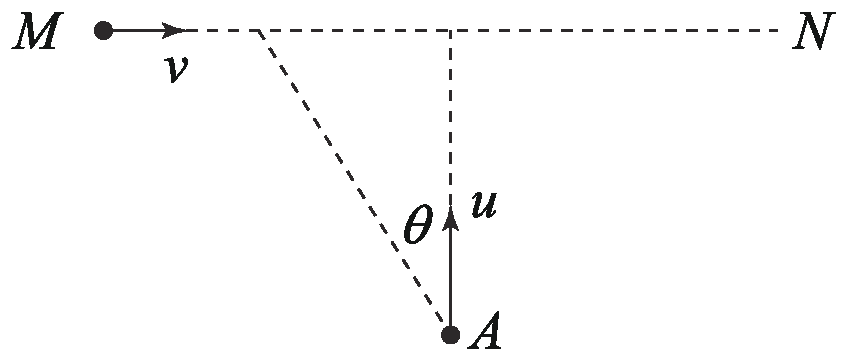
\includegraphics[width = 0.5\textwidth]{images/motion-30.pdf} 
\end{flushright}
\tagged{student}{\vspace*{4cm}}
\begin{taggedblock}{teacher}
\noindent
解析:做出船和鱼雷满足条件的运行轨迹,解三角形可知
\[
\tan\theta = \frac{vt}{ut} = \frac{v}{u},
\]
可见发射角度与它们之间的距离无关,只与速度有关。
\vspace*{3cm}
\end{taggedblock}
\end{example}

\begin{example}
足球比赛,一攻方队员在图中的$A$处沿$AX$方向传球,球在草地上以速度$v$匀速滚动,守方有一队员在图中$B$处,以$d$表示$A$、$B$间的距离,以$\theta$表示$AB$与$AX$之间的夹角,已知$\theta <90^\circ$,设在球离开A处的同时,位于B处的守方队员开始沿一直线在匀速运动中去抢球,以$v_p$表示他的速率,在不考虑场地边界限制的条件下,求出守方队员可以抢到球的必要条件。

%2.如果攻方有一接球队员个处在$AX$线上等球,以$r$表示他到$A$点的距离,求球不被原在$B$处的守方队员抢断的条件。
%
%3.如果攻方有一接球队员个处在$AX$线上等球,以$r$表示他到$A$点的距离,在球离开$A$处的同时,他开始匀速跑动去接球,以$v_r$表示其速率,求在这种情况下球不被原在$B$处的守方队员抢断的条件。
\begin{flushright}
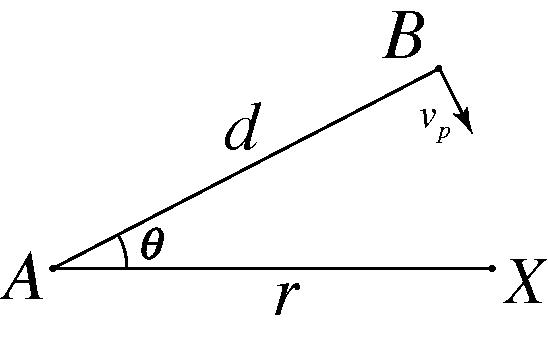
\includegraphics[width = 0.3\textwidth]{images/motion-problem-football.pdf}
\end{flushright}
\tagged{student}{\vspace*{4cm}}
\begin{taggedblock}{teacher}
\vspace*{4cm}
\noindent
解析:如上图所示,球员能够抢到球说明在某一时刻他和球处于同一位置,假设时间为$t$,这时球员跑过的距离为$v_pt$,球跑过的距离为$vt$,三角形中根据余弦定理我们有
\[
v_p^2t^2 = d^2+v^2t^2-2vtd\cos\theta,
\]
这是一个关于时间的一元二次方程
\[
(v_p^2-v^2)t^2+2dv\cos\theta t-d^2=0.
\]
能够抢到球说明这个方程有解,也就是它的判别式大于等于零:
\[
\Delta  = 4d^2v^2\cos^2\theta+4d^2(v_p^2-v^2)\ge 0,\text{可得},\qquad v_p\ge v\sin\theta.
\]
\end{taggedblock}
\end{example}

\begin{example}
两个质点$A$、$B$同时从$P$、$Q$两点出发,分别以速度$\vec{v}_{1}$沿直线$AB$和以速度$\vec{v}_2$沿PR作匀速直线运动,$QR$和$QP$的夹角为$\alpha$,开始时$PQ$两点相距$l$,求此后两质点的最短距离。
\begin{flushright}
\includegraphics[width = 0.3\textwidth]{images/motion-problem-29.pdf}  
\end{flushright}
\tagged{student}{\vspace*{4cm}}
\begin{taggedblock}{teacher}
\noindent
解析:建立一个原点在$A$点,$x$轴沿两点连线方向的坐标系,两个质点的运动可以用它们的坐标来表示,分别为
\[x_A = v_At,\qquad y_A = 0\]
\[x_B = l-v_B t\cos\alpha,\qquad y_B = v_Bt\sin\alpha.\]
这样根据勾股定理两点之间距离的平方可以表示为
\begin{eqnarray*}
d^2& =& (x_A-x_B)^2+(y_A-y_B)^2 = [l-(v_B\cos\alpha+v_A)t]^2+[v_Bt\sin\alpha]^2\\
&=& (v_B^2+v_A^2+2v_Av_B\cos\alpha)t^2-2(v_B\cos\alpha+v_A)lt+l^2
\end{eqnarray*}
是一个关于$t$的二次函数,根据二次函数图像的性质可知其对称轴位于
\[
t = \frac{v_B\cos\alpha+v_A}{v_B^2+v_A^2+2v_Av_B\cos\alpha}l
\]
处,这时它们之间的距离可将上面的时间代入距离的表达式中得到:
\[
d_{min}^2 = \left[1-\frac{(v_B\cos\alpha+v_A)^2}{v_B^2+v_A^2+2v_Av_B\cos\alpha}\right]l^2,\qquad d_{min} = \frac{v_B\sin\alpha}{\sqrt{v_B^2+v_A^2+2v_Av_B\cos\alpha}}l
\]


\end{taggedblock}
\end{example}


\begin{example}
如图所示,一个人在图中$A$点处看到一个人在水中$B$点求救,已知它在地面奔跑的速度为$v_1$,在水中游泳的速度为$v_2$,各个长度已在图中标出。
求他能够在最短时间到达落水点$B$所走的路径。
\begin{flushright}
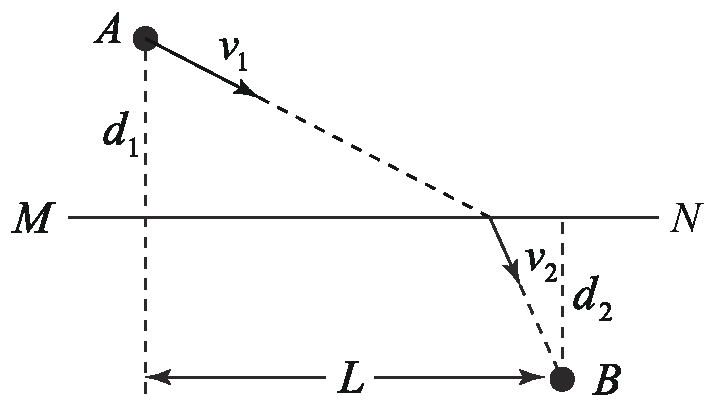
\includegraphics[width = 0.4\textwidth]{images/motion-31.pdf} 
\end{flushright}
\tagged{student}{\vspace*{3cm}}
\begin{taggedblock}{teacher}
\vspace*{2cm}
\noindent
解析:类比光的折射定律,可以得到
\[
\frac{1}{v_1}\sin\theta_1 = \frac{1}{v_2}\sin\theta_2
\]
\end{taggedblock}
\end{example}

\subsection{速度的变化:加速度}
\begin{figure}[hbtp]
\centering
\includegraphics[width=0.6\textwidth]{images/motion-theory-7.pdf}
\caption{质点运动过程中速度的变化,加速度}
\end{figure}

和一维的情况类似,平均加速度被定义为给定时间$\dt$里速度的变化率
\begin{equation}
\vec{a} = \frac{\vec{v}(t+\dt)}{\dt}=\frac{\Delta \vec{v}}{\dt},
\end{equation}
而上式在$\Delta t\rightarrow 0$的极限情况下的值为质点在$t$时刻的瞬时加速度:
\begin{equation}
\vec{a}(t) = \lim_{\Delta t\rightarrow 0}\frac{\Delta\vec{v}}{\Delta t}
\end{equation}
和速度和位移一样,一般情况下的加速度也是一个矢量,大小为速度变化量随时间的变化率,而方向给出了速度变化的方式。
因为速度是一个矢量,当它的大小或者方向发生变化时都会带来非零的加速度。




当质点在某一时刻$t$时的速度$\vec{v}(t)$和此时它的加速度$\vec{a}$同时为已知时,在此后$\dt$时间后它的速度为
\begin{equation}
\vec{v}(t+\dt) = \vec{v}(t)+\vec{a}\dt.
\end{equation}
加速度的大小和方向都不变的运动被称为{\heiti 匀加速运动}。
$t=0$时位于$\vec{r}_0$,速度为$\vec{v}_0$的做加速度为$a$的匀加速运动速度和位置随时间的变化率形式相对简单:
\begin{eqnarray}
\vec{v}(t) &=& \vec{v}_0+\vec{a}t\\
\vec{r}(r)&=&\vec{r}_0+\vec{v}_0t+\frac{1}{2}\vec{a}t^2
\end{eqnarray}



\section{抛体运动}
在地球表面附近抛出的物体在阻力可以忽略不计时的运动称之为抛体运动。
观测表明抛体运动是均加速运动,运动过程中加速度的大小等于重力加速度$g$,方向指向地面。
当初始速度的方向与地表的垂线方向一致,也就是竖直向上或向下时,抛出的质点将作直线运动,但如果初始速度有水平方向的分量时,运动的轨迹将是一条曲线,曲线的形状和大小与初速度的大小和方向密切相关,数学上将这类曲线统称为{\heiti 抛物线}
因为抛体的运动易于观察,所以我们首先集中精力研究抛体运动的一般性质和处理方法,在这里所学的方法和结果实际上能够很轻易地推广到其它的的匀加速运动中去。

在不考虑复杂因素的理想情形下,斜向抛出的物体将在一个平面内运动。
为了方便地研究抛体的运动,我们在它运动的平面内建立一个平面直角坐标系,简单起见,设坐标系的原点与抛体运动的起始点重合,$x$轴与初速度的水平分量的方向一致,称为水平方向,$y$轴垂直于地面竖直向上,称之为竖直方向。
在这样的坐标系原点处抛出质点的速度大小为$v_0$,它与水平方向的夹角定义为$\theta$,这样的两个量唯一地决定了抛体此后的运动状态。
为了定量地描写抛体的运动,我们用它在运动过程中某一时刻$t$的水平和竖直坐标值来表示它的位置。
抛体运动过程中水平和竖直方向的运动行为不同,它的水平坐标值$x$随着时间的推移均匀地增大,看上去像是在作匀速直线运动,其匀速运动的速度就是初始速度的水平分量:
\begin{eqnarray}
v_x(t)& =& v_0\cos\theta\label{eqn: motion-抛体的水平速度}\\
x(t) &=& v_0\cos\theta\cdot  t\label{eqn: motion-抛体的水平运动}
\end{eqnarray}

而在竖直坐标$y$随时间的变化关系则和以初速度的竖直分量$v_{y0} = v\sin\theta$为初速度的竖起上抛运动完全一致:
\begin{eqnarray}
v_y(t)& =& v_0\sin\theta\cdot  t-gt\label{eqn: motion-抛体的竖直速度}\\
y(t) &=& v_0\sin\theta\cdot t-\frac{1}{2}gt^2\label{eqn: motion-抛体的竖直运动}
\end{eqnarray}

像上面那样把一个空间中的曲线运动用它在某一坐标系中的各个坐标值随时间的关系来表示的过程称之为{\heiti 运动的分解},反过来如果知道了一个特定的运动过程在某一坐标系中的各个坐标随时间的关系,那么它在空间中的运动行为就被唯一地决定,这样的处理过程称为{\heiti 运动的合成}。
将一个复杂的运动首先分解为沿着各个方向的分运动,在搞清楚各个方向的分量运动的行为之后再将它们统一起来得到最终的运动是运动学中非常常用的方法。
以前面抛体运动为例,看上去抛体的运动是具有一定的复杂性的曲线运动,但将它的运动过程用它的水平和竖直坐标来描写时发现它们都满足简单的运动规律,水平方向上作匀速直线运动,而在竖直方向上稍复杂一些,也不过是竖直的落体运动。


水平和竖直方向的分运动合起来就是完整的抛体运动。
抛出物体的运动轨迹可由它们的运动方程\ref{eqn: motion-抛体的水平运动},\ref{eqn: motion-抛体的竖直运动}导出,从\ref{eqn: motion-抛体的水平运动}中解出时间
\[
t = \frac{x}{v_0\cos\theta}
\]
将它代入\ref{eqn: motion-抛体的竖直运动}当中就是可消去时间$t$从而得到抛体运动过程中任何一点处的竖直坐标和此时物体水平坐标的关系,也就是抛体的{\heiti 轨迹方程}
\begin{equation}\label{eqn: motion-抛体的轨迹方程}
y(x) = \tan\theta\cdot x-\frac{g}{2v_0^2\cos^2\theta}x^2
\end{equation}
可以看出上式当中$y$是水平坐标$x$的二次方程,这就是数学上将二次方程代表的曲线称为抛物线的原因。
进一步观察上式还可以看出所有的抛体轨迹在我们选取的坐标系中都是开口向下的抛物线,其对称轴的位置和宽度由初始条件,也就是初速度的大小$v_0$和角度$\theta$共同决定。
当初速度和抛射角取一些特殊值时的,一般的抛体运动退化成相对简单的运动形式,例如
\begin{itemize}
\item
自由落体运动:$v_0 = 0$
\item
竖直上抛运动:$v_0>0$,$\theta =  \frac{ \pi}{2}$
\item
竖直下抛运动:$v_0>0$, $ \theta = - \frac{ \pi}{2}$
\item
平抛运动: $v_0>0$, $ \theta=0$
\end{itemize}
以上就是抛体运动所满足的所有规律,灵活地使用这些基本的关系式就可以解决几乎所有和抛体运动有关的问题,以下是一些例子:

\begin{example}
网球的规则要求发球时球不能碰到球网,并且落到对方场地的指定区域(发球区)。
将发球过程简化为如下模型,整个网球场的长度为$2L$,发球区距离球网的距离为$l$,球网的高度为$h$,将球员发出球的运动简化为由高度$H$处以初速度$v_0$的平抛运动。
请证明击球的高度$H$必需大于某一给定值$H_0$才能够在规则允许的条件下将球发出,并求出$H_0$与其它已知量的关系。
\begin{flushright}
\includegraphics[width = 0.5\textwidth]{images/motion-8.pdf}
\end{flushright}
\tagged{student}{\vspace*{3cm}}
\begin{taggedblock}{teacher}
\noindent
解析:建立一个以一方端线为原点的坐标系,$x$轴指向对方场地,$y$轴指向上。
以初速度$v_0$抛出的物体的运动轨迹方程为
\[
y = H -\frac{gx^2}{2v_0^2}
\]
不碰到球网要求$x=L$时$y>h$:
\[
H-\frac{gL^2}{2v_0^2}>h,\qquad v_0^2>\frac{gL^2}{2(H-h)}
\]
而发球不出发球区则要求$x=L+l$时$y<0$:
\[
H-\frac{g(L+l)^2}{2v_0^2}<0,\qquad v_0^2<\frac{g(L+l)^2}{2H},
\]
这样联立以上两式可以看到要想满足条件需要
\[
\frac{gL^2}{2(H-h)}<\frac{g(L+l)^2}{2H},\qquad\textbf{解得}\qquad H>h\frac{(L+l)^2}{2Ll+l^2}
\]
\end{taggedblock}
\end{example}

%%%%%%%%%%%%%%%%%%%%%%%%%%%%%%%%%%
\begin{example}
将一块石头从$20\unit{m}$高的山顶上水平抛出,当石块落到地面上时,其速度方向与水平面成$45^\circ$角。
请问石块抛出时的速度是多少?
\begin{flushright}
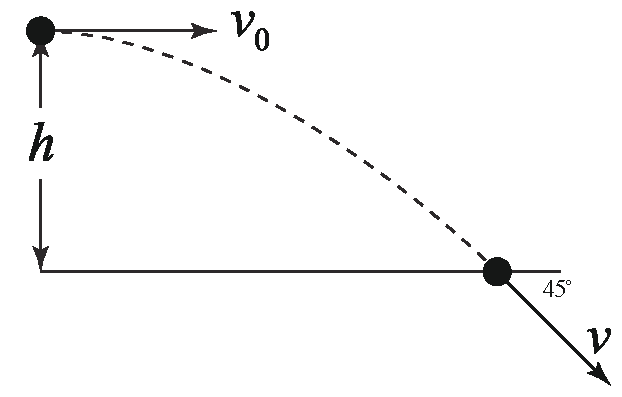
\includegraphics[width = 0.4\textwidth]{images/motion-32.pdf} 
\end{flushright}
\tagged{student}{\vspace*{2cm}}
\begin{taggedblock}{teacher}
\noindent
解析:通过抛体运动的分解可知落地时竖直方向的速度
\[
v_y = \sqrt{2gH} = 20\unit{m/s}
\]
而在运动过程中水平方向速度不变,所以如果最后以45度角撞向地面则要求水平速度$v_x = v_y = 20\unit{m/s} $。
\end{taggedblock}
\end{example}


\begin{example}
作斜上抛质点的射程被定义为当它再次落到与抛出点相同高度时的水平距离,试证明由初速度$v_0$、仰角$\theta$抛出物体的射程$S$满足
\[ S = \frac{v_0^2}{g}\sin 2\theta \]
并以此证明对于相同的初始速率$v_0$以斜向上$45^\circ$角抛出的物体射程最大。
\begin{flushright}
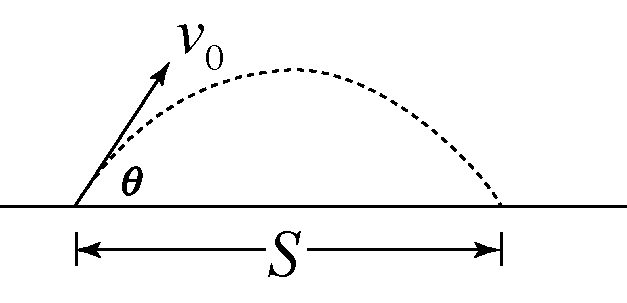
\includegraphics[width=0.4\textwidth]{images/motion-problem-2.pdf}
\end{flushright}
\tagged{student}{\vspace*{3cm}}
\begin{taggedblock}{teacher}
\noindent
解析:再次落到相同高度的时间由方程
\[
v_0\sin\theta t-\frac{1}{2}gt^2=0,\qquad t = \frac{2v_0\sin\theta}{g}
\]
给出,在这样的时间里水平方向的运动距离
\[
x = v_0\cos\theta t = v_0\cos\theta  \frac{2v_0\sin\theta}{g} = \frac{2v_0^2}{g}\sin\theta\cos\theta = \frac{v_0^2}{g}\sin 2\theta
\]
得证!
根据三角函数的性质可知,当$\theta = \frac{\pi}{4}$时上面的正弦取最大值,也就是射程达到最大,并且从中还可知最大射程
\[
S_{max} = \frac{v_0^2}{g}
\]
\end{taggedblock}
\end{example}

\begin{example}
一个以给定的初速度$v_0$,仰角为$\theta_1$抛出的物体的射程为$S$,求证以同样的初速度,仰角$\theta_2 = \pi/2-\theta_1$抛出物体的射程也是$S$,且射程相同的两个抛体在空中停留的时间乘积$t_1t_2 = \frac{2S}{g}$
\begin{flushright}
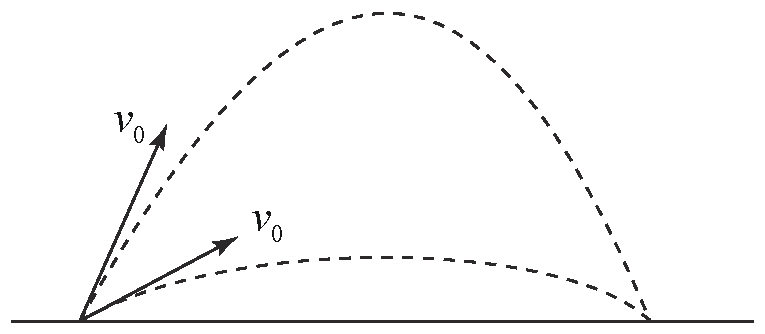
\includegraphics[width = 0.4\textwidth]{images/motion-33.pdf} 
\end{flushright}
\tagged{student}{\vspace*{4cm}}
\begin{taggedblock}{teacher}
\noindent
解析:根据前面一问得到的结果,射程和角度以及初速度大小的关系为$S = \frac{v_0^2}{g}\sin 2\theta$,相同初速率抛出的物体要想射程相同,需要有
\[
\sin 2\theta_1 = \sin 2\theta_2,\qquad \theta_1+\theta_2 = \frac{\pi}{2}.
\]
它们在空中飞行的时间分别为
\[
t_1 = \frac{2v_0\sin\theta_1}{g},\qquad t_2 = \frac{2v_0\sin\theta_2}{g}
\]
这样将它们相乘可得
\[t_1t_2 = \frac{4v_0^2}{g^2}\sin\theta_1\sin\theta_2 = \frac{2v_0^2}{g^2}\sin 2\theta_1 = \frac{2S}{g}\]
\end{taggedblock}
\end{example}



%
%\begin{example}
%求给定点$A$以相同大小的初始速率$v_0$沿不同仰角抛出的所有物体当中,当它的水平位置到达与抛出点相距$L$时可能的最大高度,以及能够到达该高度的仰角值。
%\begin{flushright}
%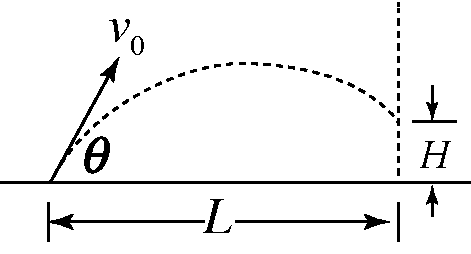
\includegraphics[width=0.3\textwidth]{images/motion-problem-3.pdf}
%\end{flushright}
%\tagged{student}{\vspace*{4cm}}
%\begin{taggedblock}{teacher}
%\noindent
%解析:
%\end{taggedblock}
%\end{example}



\begin{example}
求从图中$A$点抛出的物体能够越过距离$A$点$L$处的一个高度为$H$的障碍物所需要的最小速度。
\begin{flushright}
\includegraphics[width=0.34\textwidth]{images/motion-9.pdf} 
\end{flushright}
\tagged{student}{\vspace*{3cm}}
\begin{taggedblock}{teacher}
\noindent
解析:建立标准的坐标系,抛体的轨迹由方程\ref{eqn: motion-抛体的轨迹方程}给出。
根据题目的要求,需要它在运动到$x=L$时的高度至少为$H$,简单的分析可知最小的速度一定会出现在$y=H$时,根据三角函数的性质上面的条件等价于当把方程
\[
H = \tan\theta L -\frac{gL^2}{2v_0^2}(1+\tan^2\theta)
\]
看做是$\tan\theta$的一元二次方程时有解。
这个要求等价于方程的判别式
\[
\Delta  = L^2 - 4\frac{gL^2}{2v_0^2}(H+\frac{gL^2}{2v_0^2})\geq 0
\]
判别式在$v_0$很大时必然会小于零,而第一次出现等于零的值就意味着最小初速率,它等于零的解经过代数计算可得
\[
v_0^2 = \frac{gL^2}{\sqrt{L^2+H^2}-H}
\]
这个速度就是能够打过障碍的最小速度。
\end{taggedblock}
\end{example}


\begin{example}
对于一个从给定点$A$以给定的速率$v_0$不同角度抛出的物体来说,它所有可能到达的区域和不可能到达的区域有一条分界线,求该分解线在如图所示的坐标系中的方程。
\begin{flushright}
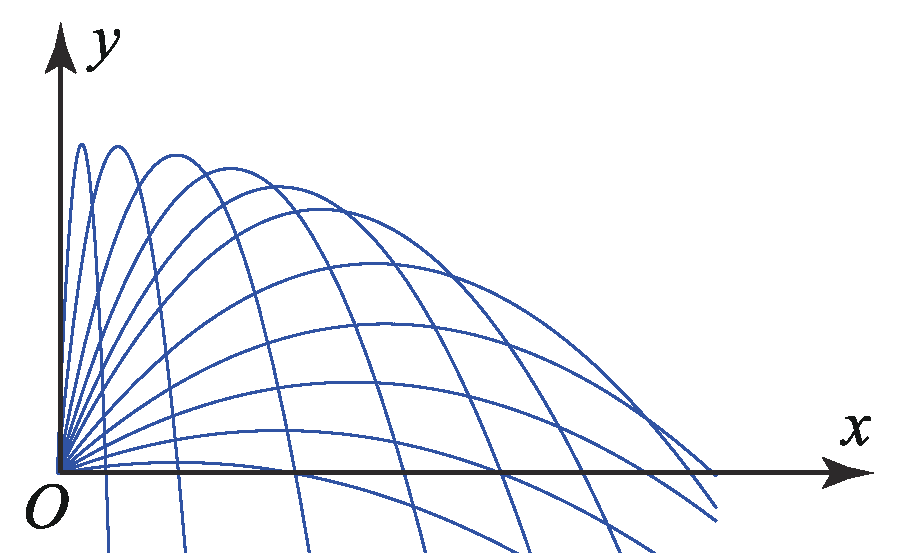
\includegraphics[width = 0.4\textwidth]{images/motion-34.pdf} 
\end{flushright}
\tagged{student}{\vspace*{4cm}}
\begin{taggedblock}{teacher}
\noindent
解析:原点抛出物体的轨迹方程\ref{eqn: motion-抛体的轨迹方程}为已知,这样对于给定的水平位置$x$处,以相同的初速率但角度不同的抛出物体当中,所能够达到的最大高度由
\[
\tan\theta = \frac{v_0^2}{gx}
\]
所给出的抛射角度给出,将这个抛射角度代入到轨迹方程中可得在给定$x$处最大高度
\[
y_max = -\frac{g}{2v_0^2}x^2+\frac{v_0^2}{2g}
\]
这就是所求的曲线方程。
\end{taggedblock}
\end{example}


\begin{example}
铅球运动员能够推出铅球的最大速度为$v_0$,肩膀距离地面的高度为$H$,求它能够推出最好成绩时铅球出手的速度方向与地面的夹角。
当$v_0 = 12.37 \unit{m/s}$,$H = 1.5\unit{m}$时求出能够得到最好成绩时的角度值以及他所获得的成绩。
\tagged{student}{\vspace*{4cm}}
\begin{taggedblock}{teacher}
\newline
解析:在初速度和高度差为已知时,想知道在给定的高度差下铅球所能够到达的最远距离,也就是上一问当中求出的曲线中$y=-H$所对应的水平坐标$x$:
\[
x = \sqrt{\frac{v_0^4}{g^2}+\frac{2v_0^2H}{g}}\simeq 23.12\unit{m}
\]
\end{taggedblock}
\end{example}

\begin{example}
在小丘上置一靶子,在炮位所在处看靶子的仰角为$\alpha$,炮与靶子间的水平距离为$L$,向目标射击时炮身的仰角为$\beta$,炮弹以什么初速度发射才能击中目标。
\begin{flushright}
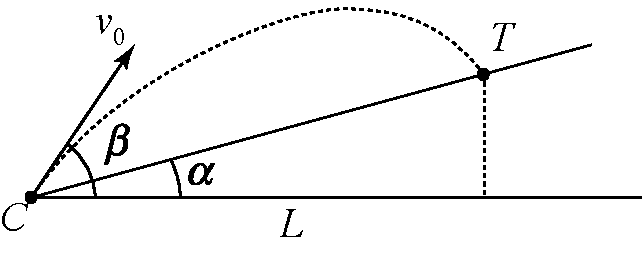
\includegraphics[width = 0.4\textwidth]{images/motion-problem-31.pdf} 
\end{flushright}
\tagged{student}{\vspace*{4cm}}
\begin{taggedblock}{teacher}
\noindent
解析:设速率为$v$则能够击中目标所需要满足的条件为
\[
L\sin\alpha = L\cos\alpha\tan\beta-\frac{gL^2\cos^2\alpha}{2v^2\cos^2\beta},
\]
解出上述方程即可得初速度
\[
v=\sqrt{\frac{gL\cos^2\alpha}{2\cos^2\beta(\cos\alpha\tan\beta-\sin\alpha)}}
\]
\end{taggedblock}
\end{example}



除了使用由方程\ref{eqn: motion-抛体的水平速度}-\ref{eqn: motion-抛体的轨迹方程}给出的代数方程以外,在解决有些问题时使用几何方法会极大降低计算量,并突出物理意义。
因为抛体运动就是匀加速度运动,在给定的时间$t$里速度的变化量就是重力加速度$g$乘以时间$t$,不要忘了速度是一个矢量,所以速度的改变量大小为$gt$,而方向指向地面。
当抛体的初始速度矢量$\vec{v}_0$被给定了以后,任一时刻$t$的速度矢量由
\begin{equation}
\vec{v}(t)=\vec{v}_0+\vec{g}t
\end{equation}
或者由图\ref{fig: motion-矢量抛体运动描写}(a)所给出的几何图形给出。
同样的道理从抛出点算起,抛体任一时刻的位移则可以用矢量表达为
\begin{equation}
\vec{r}(t)=\vec{v}_0t-\frac{1}{2}\vec{g}t^2
\end{equation}
其图形化的表示由图\ref{fig: motion-矢量抛体运动描写}(b)表示。
从中可以看出抛体的运动过程中任何时刻的位移可以看成是以初速度$\vec{v}_0$的匀速直线运动和一个自由落体运动的合成,这个图像可以极大地方便我们分析抛体的运动。
从两个图中还可以看到,当把代表位移的矢量关系图中代表自由落体的矢量放大一倍以后再与起始点连接构成的图形和代表速度矢量关系的图形相似。
\begin{figure}[hbtp]
\centering
\includegraphics[width = 0.6\textwidth]{images/motion-10.pdf}
\caption{用矢量来表示抛体运动过程中任一时刻的速度和位移,如果两个图形代表的是同一个运动过程的话,这时它处于下降阶段但依然没有回落到与抛出点相同的高度}\label{fig: motion-矢量抛体运动描写}
\end{figure}

\begin{example}
在水平地面上距离$A$点距离为$L$处有一个高为$H$的障碍物,若从$A$点抛出的物体正好通过障碍物上端时的速度方向平行于地面,求抛出的仰角$\theta$和初始速率$v_0$。
\begin{flushright}
\includegraphics[width=0.3\textwidth]{images/motion-11.pdf} 
\tagged{teacher}{\includegraphics[width = 0.4\textwidth]{images/motion-solution-tt.pdf} }
\end{flushright}

\tagged{student}{\vspace*{3cm}}
\begin{taggedblock}{teacher}
\noindent
解析:用代数的方法当然能够求解,但是如果用几何的方法则特别地简单。
如上图所示,AC代表平面距离,BC代表墙,角DAC就是抛出时速度与地面的夹角$\theta$。
代表质点位置变化的矢量关系由三角形ADB给出,而代表速度变化的矢量关系则由三角形ACD给出。
这样的图形能够满足题目所给出的条件,刚好通过顶部并且速度与地面平行。
根据要求,BA与AC的夹角需要等于墙的顶部与抛出点连线与水平面的夹角$\tan\alpha = \frac{H}{L}$,而且DB=CB由位移和速度图形的相似关系。
这样抛出速度与地面的夹角必须满足
\[
\tan\theta = \frac{2H}{L}
\]

\end{taggedblock}
\end{example}


\begin{example}
在一个与地面夹角为$\alpha$的斜面底部斜向上抛出一个物体,当它的仰角为何值时在击中斜面时速度方向刚好与斜面垂直?
\begin{flushright}
\includegraphics[width = 0.3\textwidth]{images/motion-12.pdf} 
\tagged{teacher}{\includegraphics[height=1.5in]{images/motion-solution-12.pdf} }
\end{flushright}
\tagged{student}{\vspace*{4cm}}
\begin{taggedblock}{teacher}
\noindent
解析:如右图所示,假设三角形ADC代表表示位移的矢量关系,简单的分析可知当把DC边向下延长一倍以后的三角形与表示速度的三角形相似。
根据题目中的要求,需要角$AEB = \alpha$才能够垂直击中斜面,角$CAB = \alpha$才能够刚好落到斜面上,两个条件同时满足就可以满足前面的要求。
根据几何关系角$CAE$就是直角,并且$DC=CE$,这时图中的角$BAD$就是所需要的抛出仰角。
设$AC=L$,这样
\[
\tan\theta  = \frac{DC+CB}{AB} = \frac{\frac{L}{\sin\alpha}+L\sin\alpha}{L\cos\alpha} = \frac{\frac{1}{\sin\alpha}+\sin\alpha}{\cos\alpha}
\]
就得到了角度$\theta$与斜面角度$\alpha$的关系。

\end{taggedblock}
\end{example}

因为抛体的运动非常普遍,前面的几个例子并无法包含所有的情况。
当面对其它涉及到抛体运动问题时可以通过抛体运动的一般性质综合分析,最终找到问题的答案,下面就是几个例子:

\begin{example}
一个轰炸机在距离地面高度$H$处以速度$v$匀速飞行,请你设计一个描准装置,使得当飞行员在描准镜中看到目标位于十字交叉线正中时按下投弹按扭能够使炸弹准确击中目标。
如果描准镜是一个类似于望远镜的装置,求它与竖直垂线的夹角。
假设炸弹的飞行满足抛体运动规律。
\tagged{student}{\vspace*{4cm}}
\begin{taggedblock}{teacher}
\newline
解析:投出的炸弹可以看做平抛运动,它下降$H$的高度所需要的时间$t=\sqrt{\frac{2H}{g}}$,与此同时水平飞行的距离则是$vt$,这样落地点与投弹点的连线与垂线的夹角
\[
\tan\theta = \frac{vt}{H} = \frac{v\sqrt{\frac{2H}{g}}}{H} = \sqrt{\frac{2v^2}{gH}}
\]
可见与速度和高度均有关系,在投弹时需要仔细地调整描准镜才能够准确击中目标。
\end{taggedblock}
\end{example}


\begin{example}
如图所示的多级台阶,每级台阶的长度为$d$,高度为$l$,在$A$点以水平速度$v_0$抛出一个球体,球与台阶相撞以后其水平方向速度分量保持不变,但竖直方向的速度会反向,并变成碰撞前的$e$倍,$e<1$,如果球每次碰撞前与台阶相对速度均相同且其轨迹能够形成全同的往复过程,求$v_0$的大小和每次反弹以后上升的高度。
\begin{flushright}
\includegraphics[width=0.3\textwidth]{images/motion-problem-30.pdf}
\end{flushright}
\tagged{student}{\vspace*{0cm}}
\begin{taggedblock}{teacher}
\noindent
解析:要想形成这样反复运动的过程,那么题目给出的量就不能是任意的,需要满足
\[
l = H(1-e^2)
\]
飞行的总时间就是每一段抛体在空中运行的时间
\[
T = (1+e)\sqrt{\frac{2H}{g}}
\]
要求在同样的时间里每次都向前飞行$d$的距离,从这个条件可知水平速度要满足
\[
v_0 = \frac{d}{T} = \frac{d}{(1+e)\sqrt{\frac{2H}{g}}}
\]
\end{taggedblock}
\end{example}



\begin{example}
一个球在距水平地面$h$高处以水平速度$\sqrt{2gh}$抛出,空气阻力不计。
小球每次落地反弹时水平速度不变,竖直速度大小按同样的比率$e$减小。
若自第一次反弹开始小球的运动轨迹与其在地面的投影之间所包围面积的总和为$\frac{8}{21}h^2$,求小球每次反弹竖直速度减小的比率$e$。

提示,小球每次做斜抛运动(从水平地面射出又落至地面)的轨迹与其在地面的投影之间所包围的面积等于其最大高度和水平射程乘积的$\frac{2}{3}$。
\tagged{student}{\vspace*{4cm}}
\begin{taggedblock}{teacher}
\newline
解析:13 年决赛第1题
\end{taggedblock}
\end{example}

\begin{example}
如图所示平面上有一个半径为$R$的球体,我们希望在地面上斜向上抛出一个物体击中球体的顶部。
求在不碰到球体的条件下能够击完成目标的最小的抛出速度$v_{min}$、抛出的角度$\theta_0$以及抛出点与球底部的距离$d_0$。
\begin{flushright}
\includegraphics[width = 0.3\textwidth]{images/motion-13.pdf} 
\end{flushright}
\tagged{student}{\vspace*{4cm}}
\begin{taggedblock}{teacher}
\noindent
解析:根据抛体运动的可逆性,从地面抛出的物体如果能够击中顶部的话,以相反的速度从顶部抛出则可沿着相同的轨迹落到地面,根据能量守恒,顶部抛出物体的速度越小则到达地面时的速度就越小。
这样问题就反过来变成了从顶部抛出物体,不碰到球体表面而落到地面的最小速度。
利用前一问的答案,抛体能够打到的范围是一个随着初速度增加越来越大的抛物线,初速度不够时抛物线总会和圆有交点,这样抛体无论初速度方向如何都会碰到球。
当抛物线大到能够和球相切时就有一个可能性使沿特殊的角度抛出以后它的轨迹能够与球相切,这是不碰到球的临界条件。
当包络线与圆相切时,包络面的方程和圆的方程联立时只有一个解,当速度更大时则没有解,所以可以由这个条件解出相切对应的最小速度。
两个方程分别为
\[
y=2R+\frac{v_0^2}{2g}-\frac{g}{2v_0^2}x^2 \qquad 和\qquad
x^2+(y-R)^2=R^2
\]
注意第一个方程当中坐标系原点的变化,现在抛出点位于球的顶部,所以需要将包络线上移$2R$。
联立以后可以看做是$x^2$的一元二次方程:
\[
\frac{g^2}{4v_0^4}(x^2)^2 +\left [ 1-\frac{g}{v_0^2}(\frac{v_0^2}{2g}+R) \right ]x^2+\left [  (\frac{v_0^2}{2g}+R)^2-R^2 \right ]=0
\]
其判别式为零的条件为
\[
\Delta =(\frac{1}{2}+\frac{gR}{v_0^2})^2-4\frac{g^2}{4v_0^4}(\frac{v_0^4}{4g^2}-\frac{v_0^2R}{g})=0
\]
化简之后可以解出此时速度需要满足的条件,也就是最小的可能“击中”的速度值:
\[
v_0^2 = \frac{1}{2}gR
\]
由机械能守恒可知地面的最小抛出速度为
\[
v_{min}^2=\frac{1}{2}gR+4gR = \frac{9}{2}gR
\]
其抛出点的其它性质可由轨道给出。
\end{taggedblock}
\end{example}

\section{圆周运动}
质点沿圆的运动是另一类简单曲线运动,称为{\heiti 圆周运动}。
圆周运动是非常普遍的运动形式,在游乐场可以看到大量的圆周运动的例子,在历史上很长时间里人们一直认为天体的运动也是圆周运动。
最简单的圆周运动是质点以固定的速率沿着圆周运行,这样的运动称为{\heiti 匀速圆周运动},做匀速圆周运动的质点速度大小始终不变,但是速度的方向却在不断地变化。
根据加速度的定义可以看出即使是匀速圆周运动的质点的加速度也不为零。

最方便地描写圆周运动质点的位置并不是像研究抛体运动时的平面直角坐标系,而是用运动质点与圆心的连线与一个固定方向的夹角来表示质点的位置。
如图\ref{fig: motion-圆周运动的角位置}所示当做圆周运动的质点运动到$P$点时,它与固定方向$ON$的夹角$\theta$可以唯一地确定它在圆周上的位置$P$,我们将$\theta$称为做圆周运动质点的{\heiti 角位置},习惯上规定沿着逆时间转动的方向为$\theta$增大的方向。
从某种意义上角位置和一维运动质点的坐标有很多相似之处,但也要注意它们的不同。
例如一维运动质点的位置由其坐标唯一确定,但是角位置却不同,任意与给定的$\theta$相差$2\pi$整数倍的角度实际上给出的是同样的空间位置。
例如$\theta =0$与$\theta = 2\pi$所给出的位置都是图中的$N$点。



\begin{figure}[hbtp]
\begin{minipage}[l]{0.5\textwidth}
\centering
\includegraphics[height=1in]{images/motion-14.pdf}
\caption{圆周运动质点的位置用它和圆心的连线与一固定方向的夹角表示其位置}
\label{fig: motion-圆周运动的角位置}
\end{minipage} 
\begin{minipage}[r]{0.5\textwidth}
\centering
\includegraphics[height=1in]{images/motion-15.pdf} 
\caption{角速度的正负及其对应的运动方式}
\label{fig: motion-角速度的正负及其对应的运动方式}
\end{minipage}
\end{figure}


当质点在圆周上运动时,它的角位置$\theta$会随时间的推移不断地发生变化,作匀速圆周运动的质点相同时间里角位置的变化量为常数,称为匀速圆周运动的{\heiti 角速度},它定义为单位时间里角位置随时间的变化率。
如果在$\Delta t$时间里质点转过的角度为$\Delta \theta$,这时它作匀速圆周运动的角速度$\omega$就表示为
\begin{equation}
\omega = \frac{\Delta\theta}{\Delta t},
\end{equation}
从定义可以看出当质点的圆周运动方向是使$\theta$变大的方向,则角速度为正,反之角速度为负,图\ref{fig: motion-角速度的正负及其对应的运动方式}给出了实际的例子。
如果质点在圆周运动过程中角速度时刻保持不变,则称该质点作{\heiti 匀速圆周运动}。
当初始角位置和角速度均已知的匀速圆周运动,在任意时刻$t$的角位置能够表达为
\begin{equation}
\theta(t) = \theta_0+\omega t.
\end{equation}
因为角位置的周期性,在经过一段时间后它的角位置将与初始位置的差别变成$2\pi$,很容易想像实际上质点又回到了出发点。
匀速转动一周又回到起始点所需要的时间称为匀速圆周运动的{\heiti 周期},根据定义它和角速度的关系为
\begin{equation}
\omega T = 2\pi,\qquad T = \frac{2\pi}{\omega},
\end{equation}
从中可以看出角速度越大转动的周期就越短。
另外一个用来描写转动快慢的物理量为转动的{\heiti 频率},用单位时间(通常是$1\unit{s}$)内完成转动的圈数,从定义可以看出频率$f$和周期、角速度之间必然满足关系
\begin{equation}
f = \frac{1}{T} = \frac{\omega}{2\pi}
\end{equation}
频率的单位为{\heiti 赫兹},需要注意的是它并不需要一定要求是一个整数。


匀速圆周运动质点的速度大小并不会随时间发生变化,它的速率称为匀速圆周运动的{\heiti 线速度},当沿着半径为$R$的圆弧运动质点的角速度为$\omega$时,在时间$\Delta t$里将掠过$\Delta \theta = \omega \Delta t$的角度,这样它所掠过的弧长就是$\Delta s = R \cdot \omega\Delta t$,简单的计算表明它的线速度大小
\begin{equation}
v = \omega R,
\end{equation}
可以看出线速度的大小由角速度和半径共同决定,方向则满足速度的一般性质,沿着轨迹的切线方向,对于圆来说任何一点的切线方向与该点的圆心连线方向垂直。




\begin{example}
一个质点沿半径$r=10\unit{cm}$的圆周以匀速每分钟转动30圈,求其角速度、线速度和匀速圆周运动的周期。
\tagged{student}{\vspace*{4cm}}
\begin{taggedblock}{teacher}
\newline
解析:按照各个物理量的定义逐个求解即可。
角速度
\[
\omega = \frac{30\times 2\pi}{60} = \pi\unit{rad/s}
\]

\[\text{线速度}\qquad v = \omega r = \frac{\pi}{10}\unit{m/s}\]

\[
\text{周期}\qquad T = \frac{2\pi}{\omega} = 2\unit{s}
\]
\end{taggedblock}
\end{example}

\begin{example}
如图所示,质点$A$在半径为$R$的圆周上做角速度为$\omega$的匀速圆周运动。
当它运动到圆周上一给定点$P$时有一质点$B$从圆心$O$出发沿着$OP$方向以匀速$v$匀速运动,如果两个质点能够相撞,求所有$v$的可能取值。
\begin{flushright}
\includegraphics[width = 0.3
\textwidth]{images/motion-problem-9.pdf} 
\end{flushright}
\tagged{student}{\vspace*{4cm}}
\begin{taggedblock}{teacher}
\noindent
解析:质点B运动到圆周所需要的时间$t_B = \frac{R}{v}$,如果它们能够相遇,$A$必须完成若干个完整的周期,也就是
\[
\omega t_B = n\cdot 2\pi
\]
将各个量代入并简化可知
\[
v = \frac{\omega R}{2\pi}\cdot\frac{1}{n},\qquad n=1,2,3\cdots
\]
\end{taggedblock}
\end{example}





\begin{example}
如图所示,质点$A$在半径为$R$的圆周上做角速度为$\omega$的匀速圆周运动。
当它运动到圆周上一给定点$P$时有一质点$B$从圆心$O$从静止出发沿着$OP$方向作匀加速运动,如果两个质点能够相撞,求所有加速度$a$的可能取值。
\begin{flushright}
\includegraphics[width = 0.3
\textwidth]{images/motion-problem-10.pdf} 
\end{flushright}
\tagged{student}{\vspace*{4cm}}
\begin{taggedblock}{teacher}
\noindent
解析:这时$B$运动到圆周所需要的时间变成了$t_B = \sqrt{\frac{2R}{a_B}}$,如果它能够和$A$相遇需要满足条件
\[
\omega t_B = n\cdot 2\pi
\]
代数计算表明加速度的可能取值为
\[
a_B = \frac{\omega^2R}{2\pi^2}\cdot\frac{1}{n^2},\qquad n=1,2,3\cdots
\]
\end{taggedblock}
\end{example}

\begin{example}
两个质点在半径为$R$的圆周上分别做匀速圆周运动,角速度分别为$\omega_{1,2}$,并且$\omega_2>\omega_1$,已知$t=0$时两质点在圆周上相遇,求再次相遇的时间。
如图所示,第一次相遇点位于圆心正上方$P$点处,且两质点均沿逆时针方向转动,求再次相遇时的位置与$OP$的夹角$ \theta$。
\begin{flushright}
\includegraphics[width=0.4\textwidth]{images/motion-problem-44.pdf}
\end{flushright}
\tagged{student}{\vspace*{1cm}}
\begin{taggedblock}{teacher}
\noindent
解析:这是一个圆周上的追及问题,当两质点的角速度匀为已知时,当它们之间的相对角位移达到$2\pi$时,将再次相遇。
它们之间的相对角速度自然就是它们角速度的差$\omega_2-\omega_1$,所以相遇的时刻满足
\[(\omega_2-\omega_1)t = 2\pi\,\qquad t_= \frac{2\pi}{\omega_2-\omega_1}\]
转过的角度$ \Delta \theta = \omega_1 t$。
\end{taggedblock}
\end{example}

\begin{example}
两个质点$A$和$B$分别在半径为$R_1$、$R_2$的同心圆周上做匀速圆周运动,$A$的线速度为$v_A$,$B$的线速度为$v_B$,当$t=0$时它们连线的沿长线通过圆心且两质点位于圆心的同侧,求此后它们的连线通过圆心的所有时刻。
\begin{flushright}
\includegraphics[width=0.4\textwidth]{images/motion-problem-32.pdf}
\end{flushright}
\tagged{student}{\vspace*{2cm}}
\begin{taggedblock}{teacher}
\noindent
解析:两个质点的角速度分别为$ \omega_A = \frac{v_A}{R_1}$、$ \omega_B = \frac{v_B}{R_2}$,利用上一问的结果即可。
\end{taggedblock}
\end{example}



\begin{example}
如图所示,有一个半径为$R$的圆水平放置,有一个质点$A$在其圆周上以角速度$\omega$作匀速圆周运动。
在它圆心$O$的正上方高度为$H$的$S$点以水平速度$v_0$抛出另外一个质点$B$,抛出时$A$正好位于$B$抛出的方向。
如果$B$与$A$能够相撞,则$v_0$和$H$需要满足什么条件。
\begin{flushright}
\includegraphics[width = 0.4\textwidth]{images/motion-16.pdf} 
\end{flushright}
\tagged{student}{\vspace*{4cm}}
\begin{taggedblock}{teacher}
\noindent
解析:通过对运动过程的分析可知质点下落过程所需要的时间必须是圆周运动周期的整数倍:
\[
t = \sqrt{\frac{2H}{g}} = nT = n\frac{2\pi}{\omega},\qquad H_n  = \frac{2\pi^2 g}{\omega^2}n^2
\]
水平方向上则要求
\[v_0t = R,\qquad v_n = \frac{\omega R}{2\pi} n\]
两个式子中$n$可取所有自然数。
\end{taggedblock}
\end{example}

\begin{example}
$A$、$B$两个质点在半径分别为$R_1$,$R_2$的同心圆形轨道上同向运动,$R_1<R_2$,角速度分别为$ \omega_1> \omega_2$。
从位于外侧轨道的$B$看过去$A$始终在圆心$O$点左右摆动,求在$B$看来它与$A$和$O$连线之间夹角$ \theta$的最大值以$A$相继出现在最大夹角处的时间间隔。
\begin{flushright}
\includegraphics[width=0.4\textwidth]{images/motion-problem-33.pdf}
\end{flushright}

\tagged{student}{\vspace*{4cm}}
\begin{taggedblock}{teacher}
\noindent
解析:通过做图可以发现当外侧质点看到内侧质点张角最大时,两者与圆心连线之间的夹角$\alpha$满足:
\[
\cos\alpha = \frac{R_1}{R_2},\qquad \alpha = \arccos\frac{R_1}{R_2}
\]
这时视线张角
\[
\theta = \frac{\pi}{2}-\alpha.
\]
出现最大角度有两个交替出现的周期,一个是
\[
T_1 = \frac{2\alpha}{\omega_1-\omega_2}
\]
另一个则是
\[
T_2 = \frac{2\pi-2\alpha}{\omega_1-\omega_2}
\]
分别对应于从后向前和从前向后变化的阶段。

\end{taggedblock}
\end{example}











\begin{example}
20世纪早期人们通过实验发现电子有沿着通过自身轴转动的性质。
那时的电子被看成是一个半径$r_e \simeq 3\pow{-15}\unit{m}$,实验上要求电子自转的角速度与半径平方的乘积满足
\[  \omega R^2 \approx 10^{-5}\unit{m^2/s}\]
很短时间之后电子论的创始人洛伦兹马上指出这个模型有致命的缺陷,你能够看出这里面有什么问题吗?
\tagged{student}{\vspace*{4cm}}
\begin{taggedblock}{teacher}
\newline
解析:通过计算能够表明,如果电子的运动的确由上述条件所给出,那么它的边缘运动速度远大于光速。
\end{taggedblock}
\end{example}

虽然匀速圆周运动质点的速度的大小始终不变,但是因为它速度的方向不断发生变化所以加速度并不为零。
如图\ref{fig: motion-匀速圆周运动的加速度}所示一个质点在作半径为$R$角速度为$\omega$的匀速圆周运动,在某一时刻它位于$A$点处,在随后的$\Delta t$时间之后运动到了$B$点,$A、B$两点与圆心的夹角$\Delta\theta = \omega \Delta t$,两点处的速度大小均为$\omega R$,方向沿着两点切线的方向。
为了比较两点速度的不同,将两点的速度矢量平移,使其端点重合于如\ref{fig: motion-匀速圆周运动的加速度}右图所示的$S$点处,连接两个速度矢量的端点$PQ$就是在$\Delta t$时间里速度的变化量。
在极小的时间间隔$\Delta t$内三角形$SPQ$是一个顶角$\Delta\theta=\omega\Delta t$无限地趋近于0,底角无限地趋近于直角的等腰三角形。
因为瞬时加速度的方向就是无限小时间里速度改变量的方向,所以匀速圆周运动的加速方向垂直于瞬时速度,也就是圆周切线的方向;从图中可容易看出其方向指向圆心,所以匀速圆周运动的加速度又被称为{\heiti 向心加速度}。
等腰三角形的腰长$SP=SQ=\omega R$,根据几何关系它的底边的长度为腰长与顶角的乘积:
\[
\Delta v = \omega R \Delta \theta = \omega R\cdot \omega\cdot \Delta t=\omega^2R\Delta t,
\]
可以看到向心加速度的大小与圆周运动的角速度、半径之间的关系
\begin{equation}\label{eqn: motion-a=w^2R}
a_r = \frac{\Delta v}{\Delta t} = \omega^2R,
\end{equation}
根据匀速圆周运动学变量之间的关系,向心加速度还有另外一个常用的表达式:
\begin{equation}\label{eqn: motion-a=v^2/R}
a_r = \frac{v^2}{R}.
\end{equation}
\begin{figure}[hbtp]
\centering
\includegraphics[width=0.9\textwidth]{images/motion-17.pdf}
\caption{匀速圆周运动的加速度}\label{fig: motion-匀速圆周运动的加速度}
\end{figure}



\begin{example}
(1)求一个以线速度$v = 10 \unit{m/s}$在半径$R=10\unit{m}$的圆形轨道上作匀速圆周运动质点的加速度大小。

(2)一个在半径$R = 10\unit{m}$的圆周上匀速圆周运动质点的向心加速度$a_r = 10\unit{m/s^2}$,求其圆周运动的频率。


\tagged{student}{\vspace*{4cm}}
\begin{taggedblock}{teacher}
\noindent
解析:直接根据定义进行计算。第一问
\[a = \frac{v^2}{R} = 10\unit{m/s^2}\]
第二问:
\[
f = \frac{1}{T} = \frac{\omega}{2\pi} = \frac{1}{2\pi}\unit{Hz}.
\]
\end{taggedblock}
\end{example}




\begin{example}
如果多个围绕共同圆心作匀速圆周运动质点的周期$T$的平方与它们各自的轨道半径$R$的三次方成正比:
\[ \frac{T^2}{R^3} = C, \]
其中$C$为一个常数,求它们圆周运动向心加速度与轨道半径的关系。
\tagged{student}{\vspace*{4cm}}
\begin{taggedblock}{teacher}
\newline
解析:假设轨道半径为$R$的质点匀速圆周运动的角速度为$\omega$,其周期
\[ T = \frac{2\pi}{\omega} \]
根据已知的信息可知角速度与半径之间满足
\[  \omega^2 = \frac{4\pi^2}{CR^3}, \]
这样不同半径上质点的向心加速度为
\[ a_r = \omega^2R = \frac{4\pi^2}{CR^2}, \]
可见向心加速度与它们到圆心距离的平方成反比。
当把这两个例子应用到动力学中的时候恰恰代表了两种最经典的有心力情况下的运动。
\end{taggedblock}
\end{example}

\begin{example}
如果多个围绕共同圆心作匀速圆周运动质点的周期$T$与它们各自的轨道半径$R$无关,求向心加速度与轨道半径之间的关系。
\tagged{student}{\vspace*{4cm}}
\begin{taggedblock}{teacher}
\newline
解析:和前一问几乎一模一样的做法,只不过周期和半径的关系发生了变化,简单的代数计算表明这时的向心加速度需要和轨道半径$R$成正比:
\[a_r = \frac{4\pi^2}{T^2}R\]
\end{taggedblock}
\end{example}




\begin{example}
以圆形轨道行驶的赛车速度不宜过快,否则就会打滑,已知在给定的赛道上赛车沿不同圆周作匀速运动的向心加速度的最大值均为$a$,它同时也是赛车在加速度和减速过程中的最大加速度。
考虑如图所示赛道,弯道为圆孤,内、外半径分别为$R_1$、$R_2$。
在直道上赛车以最大速度$v_0>\sqrt{aR_1}$,比较沿着赛道内侧和外侧两种方式通过弯道的时间。
\begin{flushright}
\includegraphics[width=0.4\textwidth]{images/motion-problem-34.pdf}
\end{flushright}
\tagged{student}{\vspace*{4cm}}

\begin{taggedblock}{teacher}
\noindent
解析:略
\end{taggedblock}
\end{example}

在大多数情况下,圆周运动的角速度并不是一直能够不变的,在各种因素的影响下和质点运动的速度一样,角速度也会发生变化。
把圆周运动质点的角位置在一段时间$\Delta t$内的变化量$\Delta\theta$与相应的时间间隔的比值称为$\Delta t$时间里的平均角速度,和速度类似的在极小的$\Delta t$极限下平均角速度的极限就是对应时刻的瞬时角速度:
\begin{equation}
\omega(t) = \lim_{\Delta t\rightarrow 0 }\frac{\Delta \theta}{\Delta t}
\end{equation}
当圆周运动质点在某一时刻的瞬时角速度为已知时,可以证明它的线速度和向心加速度满足和匀速圆周运动相同的规律:
\begin{equation}
v(t) = R\omega(t),\qquad a_r=\omega(t)^2R = \frac{v(t)^2}{R}
\end{equation}


和直线运动相类比,当角速度做为时间的函数为已知时,它对时间的变化率自然就被称为{\heiti 角加速度},习惯上用$\beta$来表示。
如果角速度随时间的关系用函数$\omega(t)$来表示的话,角加速度也以写为
\begin{equation}
\beta(t) = \lim_{\Delta t\rightarrow 0}\frac{\Delta \omega}{\Delta t}.
\end{equation}
当圆周运动的角加速不为零时,运动质点的加速度除了指向圆心的分量以外还会由于线速度的变化有沿着圆周切线方向的分量,称为{\heiti 线加速度}或{\heiti 切向加速度}。
简单的数学分析可知线加速度的大小
\begin{equation}\label{eqn: motion-线加速度}
a_t = R\beta
\end{equation}
这时运动质点的加速度为切向加速度和向心加速度的矢量和。
线加速度保持为常数的圆周运动称为{\heiti 匀加速圆周运动},如果$t=0$的初始时刻以角加速度$\beta$作匀加速圆周运动质点的初始角位置为$\theta_0$、初始角速度$\omega_0$的质点的角速度和角位置随时间的变化关系可以写为
\begin{eqnarray}
\omega(t)&=&\omega_0+\beta t\\
\theta(t)&=&\theta_0+\omega_0t+\frac{1}{2}\beta t^2
\end{eqnarray}
作角加速运动的质点速度的大小和方向都在不断变化,由于角加速度不为零,所以质点运动过程中沿着圆周切向的加速度分量\ref{eqn: motion-线加速度}以外,速度方向的改变同时也会导至非零的径向加速度分量,简单地分析可知向心加速度同样是由\ref{eqn: motion-a=v^2/R}给出,只不过这时式中的$v^2$在不同的时间需要取不同的数值。



\begin{example}
一质点在半径为$R=1\unit{1}$圆周上作圆周运动,$t=0$时初始角速度为$\omega_0=0$,角加速度$\beta = 1\unit{rad/s^2}$,求其边缘速度达声速$340\unit{m/s}$所需要的时间。
\tagged{student}{\vspace*{4cm}}
\begin{taggedblock}{teacher}
\newline
解析:任意时刻的线速度由
\[v = \omega(t)R = \beta R t\]
这样超过声速的时刻自然就是
\[
t' = \frac{v_S}{\beta R}\simeq 340\unit{s}
\]
\end{taggedblock}
\end{example}


%%%%%%%%%%%%%%%%%%%%%%%%%%%%%%%%%%
\begin{example}
一质点沿半径为$R$的圆轨道运动,初速度为$v_0$,其加速度方向与速度方向之间的夹角$ \theta$恒定,试求速度大小与时间的关系。
\begin{flushright}
\includegraphics[width=0.3\textwidth]{images/motion-problem-41.pdf}
\end{flushright}
\tagged{student}{\vspace*{1cm}}
\begin{taggedblock}{teacher}
\noindent
解析:【选讲】设加速度的大小为$a$,未知。在径向和横向上运动分别满足:
\[
a\cos\theta = \frac{v^2}{R},\qquad \frac{\Delta v}{\Delta t} = a\sin\theta.
\]
联立以上两式消去$a$可得速度随时间的变化关系
\[
\frac{\Delta v}{\Delta t} = \frac{v^2}{R}\tan\theta,
\]
该方程的解为
\[
v(t) = \frac{1}{\frac{1}{v_0}-\frac{\tan\theta}{R}t}
\]
\end{taggedblock}
\end{example}











\section{平面内的曲线运动}
详细地研究了抛体和圆周运动以后,我们已经积累了大量的描述物体运动的手段和技术。
在这些技术的基础上就可以着手分析更一般的运动,为简单起见假设运动物体始终保持在空间当中某个特定的平面内,称之为二维运动;后面可以看出对二维运动的研究对更复杂的三维运动的描写提供了几乎全部的术语和技术,向三维空间的推广几乎不用费任何力气。
对二维曲线运动的分析主要采取两种方法,一种是在平面直角坐标系或极坐标系中用物体在坐标系的分量随时间的变化来描写物体的运动;另一种是时刻追随运动的物体,将它所有的运动学变量在它的速度方向和垂直于速度的方向来分解从而得到运动的性质。
两种方法各有特点和优势,根据实际的问题选择合适的处理方法,下面我们就来逐一学习两种不同的描写手段。

\subsection{固定坐标系}
\begin{figure}[hbtp]
\centering
\includegraphics[width=0.5\textwidth]{images/motion-18.pdf}
\caption{用直角坐标系描写质点的曲线运动,用质点的坐标随时间的关系来决定任一时间运动质点的位置。当根据运动方程得到$t_1$时刻的两个坐标值分别为$x(t_1)$和$y(t_1)$,立刻就可以判断质点此时位于图中的$A$点处}\label{fig: motion-曲线运动的直角坐标系描写}
\end{figure}

在质点运动的平面内建立一个直角坐标系$Oxy$,其中$O$为坐标系的原点,$x、y$分别是相互垂直的两根坐标轴。
对于轴的取向并没有特别的规定,可以根据所研究对象运动的特点灵活选择。
例如处理抛体运动时选择两根轴分别平行和垂直于地面就很方便,另外在处理地面上物体的运动时将轴指向东西和南北方向可以更方便地与地理知识产生联系。
当坐标系被给定了以后,平面内任何一点的坐标就是被唯一给定的,反过来当给定了一个物体的两个坐标值以后它真实的位置也将被唯一确定。
物体的运动可以用它的两个坐标值分别与时间的关系来描写,如图\ref{fig: motion-曲线运动的直角坐标系描写}所示对于坐标系$Oxy$来说平面内质点的运动可以用它的$x$和$y$坐标与时间的函数给出:
\begin{equation}\label{eqn: motion-分量的运动方程}
x = x(t),\qquad y = y(t)
\end{equation}
$x(t)$和$y(t)$称为曲线运动分量的运动方程,无论多么复杂的曲线运动其分量看上去都是在作一维的运动,可以用一维运动的相应技术来分析分运动,最后就可以得到完整的运动。
在抛体的运动分析过程中我们已经看到,当把抛体的运动分解为水平和竖直方向的分运动以后就可以简单地分析了。
当分量的运动方程\ref{eqn: motion-分量的运动方程}为已知时,就能够得到曲线运动的其它信息。

运动物体的轨迹可以由各个时刻的位置在平面上划出的曲线所决定。
从数学上看和抛体运动类似,任意曲线运动的轨迹可以通过联立两个方向分运动的方程通过消去时间变量而得。
在有些特殊情况下很容易得到轨迹的方程,但不见得所有情况下都能够得到轨迹方程解析的表达式。



\begin{example}
已知分量的运动方程为
\[x(t) = A\cos\omega t,\qquad y(t)=A\sin\omega t\]
求运动质点的轨迹方程并在下面的坐标系中画出轨迹的示意图。
\begin{flushright}
\includegraphics[width=0.4\textwidth]{images/motion-problem-35.pdf}
\end{flushright}
\tagged{student}{\vspace*{0cm}}
\begin{taggedblock}{teacher}
\noindent
解析:很明显是一个圆,两式取平方和就可以消去时间,可以得到轨迹满足
\[x^2+y^2 = A^2\]
很明显是平面内圆的方程。
\end{taggedblock}
\end{example}

\begin{example}
已知分量的运动方程为
\[x(t) = a\cos\omega t,\qquad y(t)=b\sin\omega t\]
求运动质点的轨迹方程,并画出轨迹的示意图。
\begin{flushright}
\includegraphics[width=0.4\textwidth]{images/motion-problem-35.pdf}
\end{flushright}
\tagged{student}{\vspace*{0cm}}
\begin{taggedblock}{teacher}
\noindent
解析:轨迹是一个椭圆,将两式右边的$a$、$b$除到左边来再求平方和就可以消去时间,得到
\[\frac{x^2}{a^2}+\frac{y^2}{b^2}=1\]
是平面内椭圆的方程。
\end{taggedblock}
\end{example}



\begin{example}
一个半径为$R$的圆在平面上以做无滑动的匀速滚动,圆心速度速度为$v$,试求圆上固定一点$P$在如图所示的坐标系中$x、y$坐标随时间的函数。
\begin{flushright}
\includegraphics[width = 0.5\textwidth]{images/motion-19.pdf}  
\end{flushright}
\tagged{student}{\vspace*{4cm}}
\begin{taggedblock}{teacher}
\noindent
解析:运动学的分析表明经过$t$的时间里转过部分相对圆心的夹角为$\frac{v}{R}t=\omega t$,由几何关系可知点$P$的运动方程为
\[
x_p(t) = R[\omega t - \sin\omega t],\qquad y_p(t) = R[1-\cos\omega t]
\]
\end{taggedblock}
\end{example}




\begin{example}
已知一个在空间中运动的质点在直角坐标系$Oxyz$中的运动方程为
\[x(t) = R\cos\omega t,\qquad y(t) = R\sin\omega t,\qquad z(t) = vt \]
以上各量均为正数,试画出质点轨迹的示意图。
\begin{flushright}
\includegraphics[width=0.4\textwidth]{images/motion-problem-36.pdf}
\end{flushright}
\tagged{student}{\vspace*{0cm}}
\begin{taggedblock}{teacher}
\noindent
解析:$x-y$平面上作匀速圆周运动,在$z$方向上匀速运动,总得来看就是一个旋转上升的螺旋线。
\end{taggedblock}
\end{example}

曲线运动的速度可以由分运动速度的矢量和给出。
对于由\ref{eqn: motion-分量的运动方程}给出的运动,它在坐标轴的分速度自然为已知,这样它的速度可以由两个方向的速度合成而得。
反过来的过程也是成立的,当已知曲线运动在某一时刻的速度以后它分的分速度可由速度沿坐标轴的分量而得到。
同样的道理运动质点的加速度也等于分量的加速度的矢量和,加速度的分量等于总的加速度在对应轴的分量。

\begin{example}
现有一个质点$P$在半径为$R$的圆上作角速度为$\omega$的匀速圆周运动。
建立一个原点位于圆心$O$的平面直角坐标系,在$t=0$的时刻质点刚好处于$x$轴上,且围绕原点做逆时针转动。
求此后任意时间它在坐标轴上的投影$x(t) = R\cos\omega t$,$y(t) = R\sin\omega t$的速度和加速度。
\begin{flushright}
\includegraphics[width = 0.4\textwidth]{images/motion-35.pdf} 
\end{flushright}
\tagged{student}{\vspace*{4cm}}
\begin{taggedblock}{teacher}
\noindent
解析:当速度的分量为已知时,可以得到真实速度的大小和方向。
反过来,当知道了质点运动的速度以后,它向着各个方向投影点速度的大小和方向也能够反过来得到。
对于这个圆周运动的例子来说,沿圆周运动的速度和加速度均为已知,只需要将它们投影到各个坐标轴上就可以得到运动质点在坐标轴上投影的速度和加速度。
质点运动方程中的$\omega t$决定了投影的角度。
它在运动过程中的速度大小均为$v=\omega R$,方向沿着圆的切线;加速度大小均为$a = \omega^2R$,方向指点圆心。
通过上面的分析很容易得知,它在$x$、$y$轴的投影运动的速度和加速度分别为
\begin{eqnarray*}
&v_x = -\omega R \sin \omega t,\qquad & a_x = -\omega^2 R\cos\omega t\\
&v_y = \omega R \cos \omega t,\qquad & a_y = -\omega^2R\sin\omega t
\end{eqnarray*}

\end{taggedblock}
\end{example}





\begin{example}
试证明一个半径为$R$的圆在平面上以做无滑动的匀速滚动,圆心速度速度为$v$,当圆上固定一点$P$刚好与地面接触时的瞬时速度为零。
\begin{flushright}
\includegraphics[width = 0.4\textwidth]{images/motion-36.pdf} 
\end{flushright}
\tagged{student}{\vspace*{4cm}}
\begin{taggedblock}{teacher}
\noindent
解析:各种方法证明均可,无滑动的话自然这一点的速度必须为零。
\end{taggedblock}
\end{example}


\begin{example}
在如图所示的平面极坐标系中,一个质点的运动由方程
\[ r = vt,\qquad  \theta  = \omega t\]
给出,所有参数均为正数,试定性地画出其运动轨迹。
\begin{center}
\includegraphics[width=0.3\textwidth]{images/motion-problem-37.pdf}
\end{center}
\tagged{student}{\vspace*{0cm}}
\begin{taggedblock}{teacher}
\noindent
解析:在极坐标系中,运动质点与原点的距离随时间均匀增大,同时角度也均匀增大,可以想像到的时运动轨迹为某种形式的螺线形。
\end{taggedblock}
\end{example}


\begin{example}
在平面极坐标系中一个质点的运动由方程
\[
r = r_0 e^{\lambda t},\qquad \theta=\omega t
\]
试证明它在任何一点处的速度与它到极坐标系中心连线的夹角均为给定值,并给出该值。
已知对于任意的$x$,当其变化量$\Delta x\ll x$时,有如下的近似关系式:
\[e^{x+\Delta x}\simeq e^x(1+\Delta x)\]
\tagged{student}{\vspace*{4cm}}
\begin{taggedblock}{teacher}
\newline
解析:运动质点与中心的距离随时间指数增加,而角度则是均匀增大,轨迹也是某种形式的螺线形。
对于任意的时刻$t$以及其随后的微小时间间隔$\Delta t$,其径向距离变成了:
\[ r(t+\Delta t) =r_0 e^{\lambda (t+\Delta t)}\simeq r_0e^{\lambda t}(1+\lambda \Delta t)=r(t)(1+\lambda \Delta t)\]
这样其径向距离的变化量则是:
\[
\Delta r = r(t)\lambda\Delta t
\]
在同样的时间里,它的横向位置的变化量则是
\[ r(t)\Delta \theta  = r(t)\omega\Delta t \]
与径向距离的变化量相比可以看出
\[
\frac{\Delta r}{r \omega \Delta t} = \frac{\lambda}{\omega}=const
\]
\end{taggedblock}
\end{example}
\subsection{自然坐标系}
除了用运动平面内的直角坐标系,还可以在平行和垂直于曲线运动物体速度的方向将各个运动学变量分解。
这里将与速度相同的方向称为运动的{\heiti 切线方向},简称{\heiti 切向},故名思意切向就是运动轨迹切线的方向。
与切线垂直,指向运动轨迹弯曲的方向称为轨迹的{\heiti 法线方向},简称{\heiti 法向}。
根据运动学性质,曲线运动质点的速度只有切向分量,法向分量为零。
但是加速度则不同,作曲线运动物体加速度必然与瞬时速度方向不一致,所以加速度即有切向分量,也有法向分量。
由运动轨迹的切向和法向构成的坐标系称为{\heiti 自然坐标系},运动学变量在自然坐标系中的分量具有最明确的物理意义,但是由于曲线运动质点的切向和法向在其轨迹上不同点处的方向并不一样,所以在自然坐标系是一个方向不断发生变化的坐标系,在它里面处理运动学问题有一定的数学复杂性。


\begin{figure}[hbtp]
\centering
\includegraphics[width = 0.5\textwidth]{images/motion-20.pdf}
\caption{曲线运动速度的变化量,当$\Delta t\rightarrow 0$时可以理解加速度在自然坐标系中分量的物理含义}
\label{fig: motion-曲线运动速度的变化}
\end{figure}

假设曲线运动质点在某一给定时刻$t$时的位置矢量由$\vec{r}(t)$给出,此时的瞬时速度和瞬时加速度由矢量$\vec{v}$,$\vec{a}$给出。
在此之后的$\Delta t$时间后,它的位置和速度会发生一定的变化,如果时间间隔选取足够小的话,可以认为在$\Delta t$时间里做匀加速度直线运动,这样$t+\Delta t$时刻的速度和位置分别由
\begin{eqnarray}
\vec{v}(t+\Delta t)& = &\vec{v}+\vec{a}\Delta t\label{eqn: motion-曲线运动速度变化量}\\
\vec{r}(t+\Delta t)& =& \vec{r}(t)+\vec{v}\Delta t+\frac{1}{2}\vec{a}\Delta t^2\label{eqn: motion-曲线运动中位置的变化量}
\end{eqnarray}
给出。
我们来着重考察曲线运动物体速度的变化量,式\ref{eqn: motion-曲线运动速度变化量}的图形表示如图\ref{fig: motion-曲线运动速度的变化},从中可以看出在最一般的情况下由于非零的加速度会导致速度的大小和方向同时发生变化。
在无限小的$\Delta t$间隔里,图中的三角形$ABC$实际上是一个顶角$\Delta \theta$极其之小的三角形,在后面的推理过程中要密切注意这一点。
各条边的长度已经在图中标出,$\alpha$角代表瞬时加速度$\vec{a}$与瞬时速度$\vec{v}$的夹角。
速度大小的变化量由图中边长$AC$与$AB$的差别来表示,而速度方向的变化可以由$\Delta \theta$来表达。


在三角形$ABC$中使用余弦定理可得
\[
v(t+\Delta t) = \sqrt{v(t)^2+a^2\Delta t^2+2va\Delta t\cos\alpha}
\]
与通常的余弦定理不同的是$\alpha$是三角形的外角,所以上式中最后一项的符号为正。
在$\Delta t\rightarrow 0$的极限下可以忽略所有$\Delta t$一次方项以外的其它高次项,并将上式做近似展开:
\begin{eqnarray*}
v(t+\Delta t)&=&v(t)\left(1+2\frac{a}{v}\Delta t\cos\alpha\right)^{1/2}\\
& \simeq & v(t)\left( 1+ \frac{a}{v}\cos\alpha\Delta t \right) = v(t)+a\cos\alpha \Delta t
\end{eqnarray*}
从中可以看到速度大小的变化量
\[
\Delta v = v(t+\Delta t)-v(t) = a\cos\alpha\cdot \Delta t
\]
结合图\ref{fig: motion-曲线运动速度的变化}能够看到,速度大小的变化量等于加速度在沿速度方向的分量,也就是加速度的切向分量$a\cos\alpha$与时间间隔$\Delta t$的乘积。
也就是说加速度的切向分量能够决定曲线运动速率的变化,当加速度的切向分量与速度方向一致时运动速率将会增加,反之当加速度的切向分量与速度相反时曲线运动的速率会减小,最特殊的情况下当加速度与速度方向垂直时,运动速率不会发生任何变化,这一点在匀速圆周运动的例子中已经看到。

速度方向的变化用图\ref{fig: motion-曲线运动速度的变化}中的角度$\Delta\theta$来衡量,在小角度极限下角度的弧度值、正弦值和正切值在数字上近似相等。
在三角形$ABC$中利用正弦定理有
\[
\frac{v(t+\Delta t)}{\sin\alpha}=\frac{a\Delta t}{\sin\theta}
\]
简单的数学运算并略去更小的量以后上式可以整理成为
\begin{equation}
\Delta\theta = \frac{a\sin\alpha }{v}\Delta t
\end{equation}
从中可以看出加速度的法向分量的大小和运动速率共同决定了速度方向变化的快慢。
将上式变形可以得到
\[
a\sin\alpha = v\frac{\Delta\theta}{\Delta t},
\]
最后一个因子看上去和一个圆周运动角速度的表达式非常相似,如果假想圆周运动的线速度就是曲线运动质点在此时的速率,半径为$\rho$,那么它可以表示为
\begin{equation}
a\sin\alpha = v\frac{v}{\rho} = \frac{v^2}{\rho}
\end{equation}
它很像匀速圆周运动的向心加速度的表达式。
可以形象将曲线运动质点在其轨迹上任何一点处的运动与一个圆周运动等同起来,圆周运动的线速度就是曲线运动质点的瞬时速率,半径由上式中$\rho$给出,它由曲线运动质点速度方向的变化量所决定。
数学上将这个等效的圆周运动的圆形称作曲线运动轨迹的{\heiti 密切圆},它完全由曲线的形状所决定,图\ref{fig:Osculating_circle}给出密切圆的一个例子。
关于密切圆,有一个形象的理解。
回忆一下一些基本的几何事实:两个点唯一决定一条直线,直线上无限接近的两点之间连线的极限就是曲线的切线;与之相似的,不在同一直线上的三个点唯一地决定了一个圆,在曲线上一点的两侧取两个点,让这两个点无限地逼近给定点的过程中它们与给定点所决定的圆的极限就是曲线的密切圆。

\begin{figure}[ht]
\centering
\includegraphics[width=0.5\textwidth]{images/Osculating_circle}
\caption{曲线上任意一点处的密切圆}
\label{fig:Osculating_circle}
\end{figure}


\begin{example}
抛体运动的上升过程中加速度和速度夹角为$\underline{\qquad }$(锐,钝)角,运动速率不段$\underline{\qquad }$(增加,减小);下降过程中加速度与速度夹角为$\underline{\qquad }$(锐,钝)角,速率不段$\underline{\qquad }$(增加,减小)。
确定抛物线$y = ax^2$在$x=0$处的曲率半径。
\tagged{student}{\vspace*{4cm}}
\begin{taggedblock}{teacher}
\newline
解析:从原点出发平抛的运动方程$y=-\frac{gx^2}{2v_0^2}$,此时加速度大小为$g$,方向向下。
设此时的曲率半径为$\rho$,根据密切圆的性质可得
\[
\frac{v^2}{\rho} = g,\qquad \rho = \frac{v^2}{g}
\]
因为密切圆只与曲线形状有关,将上式与平抛轨迹方程做比较可知当抛物线用$y = ax^2$来表示时在最底点的曲率半径
\[
\rho = \frac{1}{2a}
\]

\end{taggedblock}
\end{example}

\begin{example}
评估下面这条曲线上四个点的弯曲情况,并尽可能地画出这些点的密切圆。
\begin{center}
\includegraphics[width=0.7\textwidth]{images/motion-problem-curved-lines-radius.pdf} 
\end{center}


\end{example}

\begin{example}
求长轴、短轴分别为$a、b$的椭圆在其长轴和短轴处的曲率半径。
\begin{flushright}
\includegraphics[width=0.3\textwidth]{images/motion-problem-45.pdf}
\end{flushright}
\tagged{student}{\vspace*{4cm}}
\begin{taggedblock}{teacher}
\noindent
解析:前面已经分析了椭圆轨道运动质点两个分量随时间的变化关系,当运动到长轴时加速度只有$x$分量,大小为$-\omega^2 a$,而速度只有$y$分量,大小则是$\omega b$,这样根据曲线运动的一般性质它的加速度垂直于速度,只有横向分量:
\[
\omega^2a = \frac{\omega^2b^2}{\rho_a},\qquad \rho_a = \frac{b^2}{a}
\]
同样的道理在短轴处
\[
\rho_b = \frac{a^2}{b}
\]
\end{taggedblock}
\end{example}

\begin{example}
有一个沿直线运动的质点,在$t=0$时刻速度为$v_0$并作减速运动,此后任意时刻的加速度与速度方向相反,且正比于当时的速度值$a=-kv$,求它完全停止所需要的时间和走过的总路程。
%\begin{flushright}
%\includegraphics[width = 0.2\textwidth]{images/.pdf} 
%\end{flushright}
\tagged{student}{\vspace*{4cm}}
\begin{taggedblock}{teacher}
\newline
解析:【选讲】可利用微元法讲解。
满足已知条件时速度随时间$t$和前进距离$x$变化关系为
\[
v(t) = v_0e^{-kt},\qquad v = v_0-kx
\]
\end{taggedblock}
\end{example}


\begin{example}
有一个沿直线运动的质点,在$t=0$时刻速度为$v_0$并作减速运动,此后任意时刻的加速度与速度方向相反,且正比于当时的速度值的平方$a=-\beta v^2$,求它速度随时间的变化关系。
\tagged{student}{\vspace*{4cm}}
\begin{taggedblock}{teacher}
\newline
解析:【选讲】速度随时间的变化关系为
\[
\frac{1}{v(t)} = \frac{1}{v_0}+\beta t,\qquad v(t) = \frac{v_0}{1+ v_0\beta t}
\]
\end{taggedblock}
\end{example}

\section{天体运动:太阳系的运行}
\begin{figure}[h]
\centering
\includegraphics[width=0.5\textwidth]{images/motion-Kepler_Mars_retrograde.pdf}
\caption{地球上看到的火星运动轨迹}
\label{fig:motion-Kepler_Mars_retrograde}
\end{figure}

在人类历史的很长一段时间里,人们都认为地球是宇宙的中心,太阳、月球、行星和所有的恒星都围绕地球做匀速圆周转动,这就是长期以来一直坚持的{\heiti 日心说}。
日心说在解释太阳、月球、恒星围绕地球的转动并没有什么问题,但是在试图解释行星的运行时却遇到了几乎无法克服的困难。
天文学家哥白尼指出如果假设地球和所有其它行星一起共同围绕太阳转动,那么在解释太阳系的运行时就简单了许多,经过和传统观念的长期斗争最终{\heiti 日心说}取得了胜利。
在日心说建立早期,由于观测数据不完备,也由于人们对自然界物体运动存在有一些非科学的看法,认为地球和行星围绕太阳做匀速圆周运动,但随着人们观测手段的进步并经过长期精确的天文观测以后发现行星围绕太阳的运行轨迹并不是严格的圆形,在轨道不同位置处速度也不一致。

最终天文学家开普勒在大量观测数据的基础上总结出了行星运动的三个经验定律,称为{\heiti 开普勒三定律},它们分别是
\begin{enumerate}
\item 行星的轨道是一个椭圆,太阳位于椭圆的一个焦点上。
\item 行星与太阳的连线在相同时间里扫过相同的面积。
\item 行星运行周期的平方与椭圆轨道半长轴的立方的比值对于所有行星均相同。
\end{enumerate}
按照顺序它们分别称为开普勒第一、第二和第三定律。
第一和第二定律是针对单个行星来说的,而第三定律是不同行星公转参数之间的一个关系。
开普勒定律为近代科学的发展打开了一道大门,最终牛顿在开普勒三定律的基础上建立了近代力学的体系。
我们只有先在运动学的范围内将天体的运动分析清楚以后才能够进一步地分析天体运动的其它特征。
从开普勒定律当中可以看出,行星的运动都是椭圆轨道上的曲线运动,利用前面掌握的分析曲线运动的技术就能够在一定程度上更精确地掌握行星的运动学特征,尤其是在行星在运行过程中速度和加速度的变化与它的位置,特别是和太阳的距离之间究竟满足什么样的关系。


\subsection{开普勒第一定律:椭圆}
\begin{figure}[hbtp]
\centering
\includegraphics[width=0.45\textwidth]{images/motion-ellipse-detail.pdf}  
\includegraphics[width=0.3\textwidth]{images/motion-21.pdf} 

\caption{椭圆中的各个相关几何量及其定义}\label{fig: motion-椭圆的定义}
\end{figure}


开普勒第一定律给出了轨道的形状以及和太阳的相对位置关系。
椭圆是一个之前不太熟悉的几何图形,简单地说椭圆就是圆在平面上的投影,或者说是一个被“挤扁”了的圆。
从数学上看椭圆还可以被看成是到两个给定点距离之和等于常数的所有点构成的集合。
如图\ref{fig: motion-椭圆的定义}中所给出的,这两个给定点分别为$F_1$和$F_2$,它们称为椭圆的两个{\heiti 焦点},开普勒第一定律指出当图中的椭圆代表某颗行星的轨道时,太阳必然位于$F_1$或$F_2$处。
通过对称性和椭圆的定义很容易证明,椭圆上一点到两个焦点距离之和正是椭圆当中最长的那条线$A_1A_1$的长度。
$A_1A_2$称为椭圆的{\heiti 长轴},它的中点$C$就是椭圆的中心,$CA_1=CA_2=a$称为椭圆的半长轴,它出现在开普勒第三定律当中。
与长轴相应地还有一条短轴,在图中用$CB_1=CB_2=b$表示,长轴和短轴的长度就唯一确定了椭圆的形状,并且从中可以看出当长轴与短轴长度相同时椭圆就退变成了一个圆。
除了长轴和短轴以外,中点到焦点的距离$CF_1=CF_2=c$也是椭圆的一个重要的特征量,它称为椭圆的{\heiti 半焦距},自然两焦点之间的距离就是椭圆的{\heiti 焦距}。
半焦距$c$与半长轴$a$的比值称为椭圆的偏心率
\begin{equation}
e = \frac{c}{a},
\end{equation}
偏心率是描写椭圆更圆一些或更扁一些的物理量,$e=0$的极限情况下椭圆就退化为一个圆,从这个角度来说圆可以看做是偏心率为零的椭圆,对于椭圆来说$0<e<1$,偏心率越大椭圆就越扁,反之偏心率越小椭圆就越圆。
建立图\ref{fig: motion-椭圆的定义}所示的平面直角坐标系,原点和椭圆的中点重合,$x$轴和$y$轴分别与长轴和短轴重合,这样椭圆上所有的点满足方程
\begin{equation}
\frac{x^2}{a^2}+\frac{y^2}{b^2}=1.
\end{equation}




\begin{example}
证明在椭圆当中$a^2=b^2+c^2$,在此基础上将半短轴长度$b$用$a$和$e$表示出来。
\begin{flushright}
\includegraphics[width = 0.3\textwidth]{images/motion-37.pdf} 
\end{flushright}
\tagged{student}{\vspace*{2cm}}
\begin{taggedblock}{teacher}
\noindent
解析:由短轴的顶点、中心点和一个焦点做一个直角三角形,三条边的长度分别为$a$、$b$和$c$,在三角形当中使用勾股定理可以证明该结论。
进一步可以根据偏心率的定义可知
\[
b=\sqrt{a^2-c^2}=\sqrt{a^2-a^2e^2} = a\sqrt{1-e^2}
\]
\end{taggedblock}
\end{example}

\begin{example}
用椭圆的半长轴$a$和偏心率$e$写出椭圆面积的表达式。
\tagged{student}{\vspace*{4cm}}
\begin{taggedblock}{teacher}
\newline
解析:椭圆是圆的投影,所以它的面积也等于圆面积在平面上的投影。
简单的分析可知椭圆面积$S=\pi ab$,根据前面一问的答案可知
\[S=\pi a b = \pi a^2\sqrt{1-e^2}\]
\end{taggedblock}
\end{example}

\begin{example}
行星轨道上距离太阳最近的点称为近日点,与太阳相距最远的点称为远日点。
求当一颗行星在半长轴为$a$,偏心率为$e$的椭圆轨道上运动时近日点和远日点的距离。
\begin{flushright}
\includegraphics[width = 0.4\textwidth]{images/motion-38.pdf} 
\end{flushright}
\tagged{student}{\vspace*{4cm}}
\begin{taggedblock}{teacher}
\noindent
解析:根据椭圆中各个量的定义,半长轴为$a$,偏心率为$e$时轨道的半焦距
\[
c = ae
\]
从几何上可以看出近日点和远日点与太阳的距离分别为
\[ r_1 = a(1+e),\qquad r_2 = a(1-e) \]
\end{taggedblock}
\end{example}






\subsection{开普勒第二定律}
\begin{figure}[hbtp]
\centering
\includegraphics[width=0.7\textwidth]{images/motion-22.pdf}
\caption{开普勒第二定律:相同时间里矢径扫过相同的面积}\label{fig: motion-开普勒第二定律解释}
\end{figure}


开普勒第一定律给出了行星轨道的形状和太阳的位置,第二定律告诉了我们轨道上的行星位置是如何随时间变化的。
与直线运动不同的是做曲线运动的行星与太阳连线(矢径)扫过的面积与时间成正比,一段时间矢径扫过的图形为一个类似于图\ref{fig: motion-开普勒第二定律解释}左面所示的扇形的几何图形$SP_1P_2$,其面积并不容易计算。
但在一段极其之小的时间里行星的运动可以近似地看成是匀速直线运动,在这样的小的时间里行星矢径扫过的面积可以近似地看成一个顶角很小的三角形,它的面积可以通过行星的速度以及它对太阳的位置所决定。

如图\ref{fig: motion-开普勒第二定律解释}右图所示,在某一时刻$t$行星位于轨道上的$P$点处,它的速度与椭圆相切,大小为$v$,已在图中标出。
在随后的$\Delta t$时间内,它的速度近似地认为没有发生太大的变化,其位置$Q$与$P$的连线可以看做一条直线,其长度为行星线速度与时间的乘积$v\Delta t$。
在此期间矢径扫过的面积等于三角形$SPQ$的面积,如果此时$P$点与太阳的距离为$r$时,三角形$SPQ$的面积
\[
\Delta S = \frac{1}{2}v\Delta t\cdot r\cdot \sin\theta
\]
这时矢径扫过面积随时间的变化率与行星运动学变量之间的关系为
\begin{equation}
\frac{\Delta S}{\Delta t} =\frac{1}{2} vr\sin\theta.
\end{equation}
开普勒第二定律表明上式的右边对于行星轨道的任何位置均为常数。
也就是说行星在它轨道上任何一点上的速度、它与太阳的距离以及速度方向与矢径方向夹角的正弦的乘积为常数
\begin{equation}
vr\sin\theta = \textmd{常数}.
\end{equation}
上式中同时包含了三个运动学变量,在数学处理上有一定的复杂性。
如图\ref{fig: motion-开普勒第二定律应用到近日点和远日点}所示当行星运动到近日点和远日点时,速度和矢径方向垂直,可以很容易地得到这两点之间的一个关系:
\begin{equation}
v_1r_1=v_2r_2
\end{equation}
其中$v_{1,2}$,$r_{1,2}$分别代表近日点、远日点处的速率和距离,这个关系虽然简单,但是对于处理行星运动问题来说非常重要。

\begin{figure}[hbtp]
\centering
\includegraphics[width=0.5\textwidth]{images/motion-23.pdf}
\caption{开普勒第二定律在近日点和远日点处的应用}\label{fig: motion-开普勒第二定律应用到近日点和远日点}
\end{figure}

\begin{example}
天文观测数据表明,地球近日点为$147\pow{6}\unit{km}$,远日点$152\pow{6}\unit{km}$,她在近日点的速度为$30.29\unit{km/s}$,求地球轨道的偏心率以及它在远日点的速度。
\tagged{student}{\vspace*{4cm}}
\begin{taggedblock}{teacher}
\newline
解析:根据近日点、远日点长度的公式,令两点距太阳距离$r_1<r_2$,写义$k=r_1/r_2$,有
\[ \frac{1-e}{1+e} = \frac{r_1}{r_2}=k,\qquad e = \frac{1-k}{1+k}\simeq 0.0167. \]
从中可以看出地球的轨道很圆。
又通过开普勒第二定律可知
\[v_1r_1 = v_2r_2,\qquad v_2 = \frac{r_1}{r_2}v_1\simeq 29.4\unit{km/s}\]
\end{taggedblock}
\end{example}

\begin{example}
当行星运动轨道的半长轴为$a$,偏心率为$e$且其通过近日点和远日点时的速度分别为$v_{1,2}$,求证它公转的周期
\[  T = \frac{2\pi a}{v_1}\sqrt{\frac{1+e}{1-e}}  = \frac{2\pi a}{v_2}\sqrt{\frac{1-e}{1+e}} \]
\tagged{student}{\vspace*{4cm}}
\begin{taggedblock}{teacher}
\newline
解析:根据所给数据,椭圆的半短轴长度和面积分别为
\[b = a\sqrt{1-e^2},\qquad S = \pi a b = \pi a^2\sqrt{1-e^2}.\]
它通过近日点的速度为已知,而近日点与太阳的距离则是$r_1 = (1-e)a$,这样单位时间时矢径扫过的面积自然就是
\[
\frac{\Delta S}{\Delta t} = \frac{1}{2}(1-e)v_1a
\]
根据开普勒第二定律,所有时间里扫过的面积都相同,所以行星公转周期就是总面积除以面积速度:
\[
T = \frac{S}{\frac{\Delta S}{\Delta t}} = \frac{\pi a^2\sqrt{1-e^2}}{\frac{1}{2}(1-e)v_1a} = \frac{2\pi a \sqrt{1-e^2}}{v_1(1-e)}=\frac{2\pi a \sqrt{1-e^2}}{v_2(1+e)}
\]
稍加变形就可以得到最终结论。
\end{taggedblock}
\end{example}

\begin{example}
试证明:匀速直线运动的物体与任一固定点连线在相同时间里扫过相同的面积。
\tagged{student}{\vspace*{4cm}}
\begin{taggedblock}{teacher}
\newline
解析:只需要画出固定的点和一个匀速直线运动的质点在两个相邻时刻走过的轨迹,并且找到它与固定点连线扫过的面积的三角形,就可以发现它们是同底等高的两个三角形,自然面积是相等的。
\end{taggedblock}
\end{example}

因为行星是在椭圆轨道上运动,所以它们速度的大小和方向总是不断地发生变化,这样加速度永远不为零。
行星运动的加速度为我们探索其运动定律提供了丰富的线索,开普勒第二定律的一个结论就行星的轨道运动过程中加速度的方向永远指向太阳!
下面我们就来看一下这个结论是如何通过运动学的分析得到的。

和一般的曲线运动相似,只要我们研究的是极短时间里的运动,那么这段时间里运动物体的速度和加速度的变化量就可以忽略不计,从而可以看成是匀加速运动。
从\ref{eqn: motion-曲线运动中位置的变化量}可以看出,在极小的时间里,曲线运动的质点位置变化可以看成是以当前的速度进行的匀速直线运动和以当前的加速度做的初速度为零的匀加速度运动的合成,两个分运动的方向分别与瞬时速度和瞬时加速度方向一致。

\begin{figure}[hbtp]
\centering
\includegraphics[width=0.6\textwidth]{images/motion-24.pdf}
\caption{将行星运动切割成无限多的部分可以证明开普勒第二定律}\label{fig: motion-开普勒第二定律的证明}
\end{figure}

如图\ref{fig: motion-开普勒第二定律的证明}所示,假设行星运动到轨道上的$A_1$点,此时的速度大小为$\vec{v}_1$,指向$A_1B_1$方向,那么假设它的加速度为零的话在$\Delta t$时间之后它将运动到$B_1$点且$A_1B_1 = v_1\Delta t$。
但是由于非零的加速度行星真实的运动还需要在矢量$A_1B_1$的基础上叠加上由于加速度带来的位移,假设加速度的大小为$a_1$,指向此时太阳所处的位置$S$,在目前对它的大小不做特殊的规定,加速度引起的位置变化量由图中的矢量$B_1A_2$来给出,其大小等于$\frac{1}{2}a_1\Delta t^2$,由于$A_2B_1$平行于$SA_1$,所以三角形$SA_1A_2$的面积与三角形$SA_1B_1$(图中未画出)的面积相等。
最后在非零的速度和加速度共同影响下行星真实的运动由$A_1A_2$给出,它的长度与时间$\Delta t$的比值可以看成是在加速度影响下行星运动到$A_2$点的速率,$A_1A_2$的方向自然就是$A_2$点行星的速度方向。

当行星运行到$A_2$点后,假如它的加速度为零,将以当前的速度做匀速直线运动到图中的$B_2$点且$A_1A_2=A_2B_2$,如果在$A_2$点的加速度方向指向此时行星与太阳连线方向$A_2S$的话,在相同的$\Delta t$时间以后行星所处的位置$A_3$与$B_2$的连线与$A_2S$平行,大小等于$\frac{1}{2}a_2\Delta t^2$,其中$a_2$为行星在$A_2$点上加速度的大小。
根据三角形的几何性质,三角形$SA_2A_2$与$SA_2B_2$同底等高,所以它们面积相同;同理三角形$SA_2B_2$与$SA_1A_2$同底等高,所以它们的面积也相同,联合以上两个事实可知三角形$SA_1A_2$的面积与$SA_2A_3$相等。
因为三角形$SA_1A_2$与$SA_2A_3$是行星在相同的时间间隔里矢径扫过的面积,根据以上的分析可以知道假如在$A_1$和$A_2$点上的加速度的方向均指向当时太阳的方向,无论加速度的大小如何矢径扫过的面积均相同。
将同样的推理持续地应用到此后的运动过程可以得出结论:在行星运动的加速度时刻指向太阳的情况下,行星与太阳的连线在相同时间里扫过相同的面积,也就是开普勒第二定律。

\begin{example}
前面已经证明了如果行星的加速度时刻指向太阳的话,行星矢径在相同时间里扫过相同的面积。请证明上述结论的逆命题,即当行星与太阳的连线在相同时间里扫过面积相同时,行星在轨道上任意时刻的加速度必须指向太阳。
\tagged{student}{\vspace*{4cm}}
\begin{taggedblock}{teacher}
\newline
解析:将前面的推理反过来说一遍,在极小的相同时间里只有由非零的加速度带来的运动状态的变化能够满足等面积定律。
\end{taggedblock}
\end{example}




\begin{example}
根据开普勒第二定律证明:行星在近日点$A$和远日点$B$处的加速度$a_{A,B}$的比值反比于近、远日点距离的比值:
\[\frac{a_A}{a_B} = \frac{r_B^2}{r_A^2},\]
即近远日点的加速度反比于与太阳距离的平方。
\tagged{student}{\vspace*{4cm}}
\begin{taggedblock}{teacher}
\newline
解析:因为近、远日点在椭圆上是对称点,这两点处的曲率半径相同,均为$\rho = b^2/a$。
因为加速度必然指向太阳,并且在近、远日点处的速度与太阳的向径垂直,所以只有向心加速度。
向心加速度的大小
\[a = \frac{v^2}{\rho}\]
因为曲率半径相同,所以两点处的加速度的比值就是速度平方的比值:
\[a_A/a_B = v_A^2/v_B^2 = r_B^2/r_A^2\]
\end{taggedblock}
\end{example}


\begin{example}
更细致的天文观测表明,行星与太阳的连线相同时间里扫过的面积并不严格相等。
假设某一段时间里木星与太阳的连线在单位时间里扫过的面积随时间增加,试在图中定性地给出此时木星加速度的方向,其中箭头表示木星公转的方向。
\begin{flushright}
\includegraphics[width = 0.3\textwidth]{images/motion-problem-25.pdf} 
\tagged{teacher}{\includegraphics[width = 0.3\textwidth]{images/motion-problem-25-solution.pdf} }
\end{flushright}
\tagged{student}{\vspace*{0cm}}
\begin{taggedblock}{teacher}
\noindent
解析:加速度指向轨道弯曲的方向,但是由于此时木星与太阳连线扫过面积速度随时间增加,从前面的分析可知它的加速度必需有沿着运动方向向前的分量,所以最后的结果如图所示。
\end{taggedblock}
\end{example}

\begin{example}
当木星和土星的相对位置关系如左图所示,其中$S$代表太阳,$J$代表木星而$Sat$表示土星,它们沿逆时针方向围绕太阳公转。长期的天文观测表明当它们之间的位置关系如左图时木星与太阳的连线扫过的面积随时间增加,而当它们的位置如右图所示时,木星与太阳连线扫过的面积随时间减小,从中你能够得到什么样的结论?
\begin{flushright}
\includegraphics[width = 0.6\textwidth]{images/motion-problem-26.pdf} 
\end{flushright}
\tagged{student}{\vspace*{2cm}}
\begin{taggedblock}{teacher}
\noindent
解析:从前一问的结论可知,当土星位于木星运行前方时,木星的加速度有向前的分量;反过来土星位于木星后方时木星的加速度有向后的分量,这实际上是万有引力的结论。
\end{taggedblock}
\end{example}


\subsection{开普勒第三定律}

开普勒第三定律给出了不同行星公转周期与它们椭圆轨道半长轴之间的关系,由于这里面涉及到复杂的数学运算,以我们目前的数学和物理知识还无法严格地分析。
实际的天文观测表明,虽然各个行星的运行轨道都是椭圆,但实际上多数行星椭圆轨道的偏心率都很小,也就是说多数行星的轨道都非常接近于圆。
表\ref{table: motion-太阳系行星数据}给出了太阳系八大行星轨道的半长轴、偏心率和周期的观测数据,从中可以看出除了水星以外的其它行星轨道都很接近于圆形。
其中长度的单位为{\heiti 天文单位},它被定义为地球到太阳的平均距离,由于地球公转轨道也十分接圆形,所以地球的半长轴大约就是一个天文单位;另外为了不让数字变得很大,各个行星的周期用年来表示,自然地球公转的周期就是一年。


\begin{table}[ht]
\begin{center}
\begin{tabular}{|c|c|c|c|c|c|c|c|c|}
\hline 
行星 & 水星 & 金星 & 地球 & 火星 & 木星 & 土星 & 天王星 & 海王星 \\ 
\hline 
半长轴(Au) & 0.39 & 0.72 & 1 & 1.5 & 5.2 & 9.5 & 19 & 30 \\ 
\hline 
偏心率 & 0.21 & 0.0068 & 0.017 & 0.093 & 0.048 & 0.054 & 0.047 & 0.0086 \\ 
\hline 
周期(年) & 0.24 & 0.62 & 1 & 1.88 & 11.86 & 29.45 & 84.02 & 164.79 \\ 
\hline 
\end{tabular} 
\caption{太阳系八大行星半长轴、偏心率和公转周期的观测值}\label{table: motion-太阳系行星数据}
\end{center}
\end{table}


如果将行星的轨道用圆做近似的话,各个行星的公转就被简化为以太阳为中心的匀速圆周运动,这时开普勒第三定律可以写成
\begin{equation}\label{eqn: motion-kepler's 3rd law for circal motion}
\frac{T^2}{R^3}=C
\end{equation}
其中$T$和$R$分别代表行星公转的周期和半径,$C$是一个常数,与行星的任何性质均无关。
通过开普勒第三定律能够给出各个行星之间运动学参数之间丰富的联系。

\begin{example}
由开普勒第三定律推出沿半径为$R$的圆形轨道公转行星的线速度$v$和角速度$\omega$。
\tagged{student}{\vspace*{4cm}}
\begin{taggedblock}{teacher}
\newline
解析:周期$T$可以写成$T = \frac{2\pi R}{v}$,将它代入第三定律的表达式\ref{eqn: motion-kepler's 3rd law for circal motion}可得
\[
\frac{4\pi^2 R^2}{v^2 R^3} = \frac{4\pi^2}{v^2R} = C
\]
这时可以解出:
\[
v^2 = \frac{4\pi^2}{CR},\qquad v = \sqrt{ \frac{4\pi^2}{CR}}
\]
根据速度和角速度的关系可得角速度满足
\[
\omega = \frac{v}{R} = \sqrt{ \frac{4\pi^2}{CR^3}},\qquad \omega^2 = \frac{4\pi^2}{CR^3}
\]
\end{taggedblock}
\end{example}


\begin{example}
据报道,天文学家发现在冥王星外还可能存在有一个较大的围绕太阳转动的天体,通过观测发现它的周期约为288年,假设该行星绕太阳做匀速圆周运动,求它与太阳的距离是地球距太阳距离的多少倍?
\tagged{student}{\vspace*{4cm}}
\begin{taggedblock}{teacher}
\newline
解析:开普勒第三定律的直接应用,如果以年和天文单位为时间和长度的计量单位,那么:
\[
\frac{T^2}{R^3} = 1,\qquad R = 43.61\unit{AU}
\]
\end{taggedblock}
\end{example}

\begin{example}
利用开普勒第三定律给出沿半径为$R$的圆形轨道公转的行星加速度与半径的关系。
\tagged{student}{\vspace*{4cm}}
\begin{taggedblock}{teacher}
\newline
解析:前面已经有了速度的表达式,直接利用匀速圆周运动加速度的表达式可得
\[
a = \frac{v^2}{R} = \frac{4\pi^2}{CR^2}
\]
\end{taggedblock}
\end{example}


\begin{example}
两颗行星围绕太阳公转轨道的半长轴和偏心率分别为$A_{1,2}$和$e_{1,2}$。
试证明两颗行星分别运行到远日点时,它们加速度的比反比于它们各自的远日点距离的平方,即
\[  \frac{a_1}{a_2} = \frac{1/r_1^2}{1/r_2^2} \]
其中$a_{1,2}$分别为两个行星在远日点的加速度,$r_{1,2}$分别为两颗行星远日点与太阳的距离。
\tagged{student}{\vspace*{4cm}}
\begin{taggedblock}{teacher}
\newline
解析:根据开普勒第二定律以及两颗行星的轨道参数,可知两个行星的轨道周期分别为
\[ T_1 = \frac{2\pi A_1}{v_1}\sqrt{\frac{1-e_1}{1+e_1}},\qquad T_2 = \frac{2\pi A_2}{v_2}\sqrt{\frac{1-e_2}{1+e_2}}\]
其中$v_{1,2}$分别是两行星运行到远日点时的速度。
开普勒第三定律给出,两行星周期$T_{1,2}$的平方与半长轴$A_{1,2}$立方的比值为常数,设此常数为$C$,那么我们有
\[
\frac{4\pi^2}{v_1^2 A_1}\frac{1-e_1}{1+e_1} = C
\]
同理角标1换成2也成立。

当它们各自位于远日点时,根据前面的分析,加速度方向指向太阳,大小$a = \frac{v^2}{\rho}$,其中$\rho$为远日点的曲率半径,大小等于$\rho = b^2/a = (1-e^2)a$。
这样
\[
a_i = \frac{v_i^2}{(1-e_i^2)a_i}  = \frac{4\pi^2}{C}\frac{1}{a_i^2(1+e_i)^2} = \frac{4\pi^2}{C}\frac{1}{r_i^2},\qquad i=1,2\]
其中$r_i$为行星远日点距离,得证。
从中也可以看出,只要开普勒第三定律成立,这个结论可以推广到所有的行星上去。
结合前面第二定律中的问题,这个结论可以进一步推广到近日点和远日点上。
但以这种方法无法还暂时没办法推广到轨道上所有的位置。
\end{taggedblock}
\end{example}

\begin{example}
根据由表\ref{table: motion-太阳系行星数据}给出的太阳系行星观测数据完成下表,并给出开普勒第三定律\ref{eqn: motion-kepler's 3rd law for circal motion}中的常数值。
\begin{center}
\begin{tabular}{|c|c|c|c|c|c|c|c|c|}
\hline 
行星 & 水星 & 金星 & 地球 & 火星 & 木星 & 土星 & 天王星 & 海王星  \\ 
\hline 
$T^2$ &   &   &   &   &   &   &   &  	 \\ 
\hline 
$a^3$ &   &   &   &   &   &   &   &   \\ 
\hline 
$T^2/a^3$ &   &   &   &   &   &   &   &   \\ 
\hline 
\end{tabular} 
\end{center}

\tagged{student}{\vspace*{4cm}}
\begin{taggedblock}{teacher}


\end{taggedblock}
\end{example}

\begin{example}
火星是人类将要登陆的下一个目标。
地球和火星围绕太阳运动的轨道都可近似看作圆形,下图中两个虚线圆周分别表示地球和火星的运行轨道,二者绕行方向相同。
已知地球绕太阳一周的时间为365日,火星绕太阳一周的时间为687日。
要想在地球上发射飞船到达火星,并且发射时耗费燃料最少,应使飞船沿图中虚线表示的椭圆轨道飞行半周,恰与火星轨道相切,此时如果火星恰好运动到该处即可登陆火星。
请通过计算后在力中大致画出发射飞船时刻火星所处的位置以及飞船登陆火星时刻地球所处的位置。
\begin{flushright}
\includegraphics[width=0.4\textwidth]{images/motion-problem-38.pdf}
\end{flushright}
\tagged{student}{\vspace*{1cm}}
\begin{taggedblock}{teacher}


\vspace*{4cm}
\noindent
解析:不仅仅是行星,人造卫星的运动也满足第三定律,根据题意我们知道它的轨道半长轴
\[a = \frac{R_E+R_M}{2}\]
这样根据第三定律可知从地球轨道运动到火星轨道所需要的时间,进而求出发射卫星时火星的位置。

\end{taggedblock}
\end{example}










\section{相对运动,参考系}
一个很显的事实就是地球在不停地自转,与此同时又以大约一年为周期围绕太阳作公转,近代的天文观测表明,太阳也不是绝对静止的,而是以极高的速度围绕银河系的中心作转动。
所有的物体每时每刻都处于不停的运动状态当中。
正因为如此,作为物质运动观测者的我们也不可避免地处于复杂的运动状态,曾经人们希望通过某种方法得到物体严格、绝对的运动,但随着时间的推移人们逐渐发现这样的目标实际上是无法达到的。
古老的争论最终的答案反而是简单的:正是因为绝对静止的物体是不存在的,所以任何人,或者更准确地说观测者都有权认为自己是不动的,有权用自己的方式描写所有其它物体的运动!
这样不同的观测者对于同一个物体运动的描写方式其实是可以不同,而在运动学中,只要知道了两个不同观测者之间相对运动的情况,也就是两个运动着的观测者之中的某一个看到的第二个观测者的运动状态为已知时,它们所看到的同一个物体的运动方式之间就有确定的联系。



无论是直角坐标系或极坐标系,都需要有一个原点。
也就是说总是需要一个空间中的给定点才能够建立这些坐标系,没有这样一个给定的点坐标系的建立也就无从谈起。
运动学中,选择一个或一些被认为是静止不动物体的过程称为选择了{\heiti 参考系},在参考系中可以取一个点以及通过该点一些明确定义的方向建立{\heiti 坐标系}来描写其它物体的运动。
在运动学中参考系和坐标系的选取具有相当的任意性,用不同的坐标系来描写质点的运动均是合法和可行的,只不过坐标系选择合理的话描写起来会方便一些。
相同于不同的坐标系对同一质点运动的描写方式之间是有确定的关系,这种关系与被描写质点的运动无关,只依赖于两个坐标系之间的关系。


\subsection{在不同坐标系中描写运动}
\begin{figure}[hbtp]
\centering
\includegraphics[width=0.6\textwidth]{images/motion-28.pdf}
\caption{用两个相对静止的坐标系描写同一质点的运动}\label{fig: motion-用两个相对静止的坐标系描写同一质点的运动}
\end{figure}

最简单的情况下,考虑用图\ref{fig: motion-用两个相对静止的坐标系描写同一质点的运动}所示的两个一维坐标系$Ox$和$Ox'$来描写同一个物体的一维运动,两个坐标系相对静止,但是两个坐标系的原点并不重全,坐标系$Ox'$的原点位于$Ox$系当中$x=x_0$处。
当运动质点在某一时刻位于图中的$P$点时,它在两个坐标系中的坐标值并不相同,但是简单的分析即可看出无论质点位于何处,它在两个坐标系中的坐标值均满足关系式
\begin{equation}
x' = x - x_0
\end{equation}
物理上将上式称做两个坐标系之间的{\heiti 坐标变换}。
当质点$P$处于运动状态时,它的速度和加速度可以相对于两个参考系分别描写。
如果我们假设两个参考系中所用的时间都是相同的,那么可以证明质点相对于两个参考系的速度一致。
同样的道理质点的加速度在两个参考系中也是一样的。

当两个参考系之间有相对运动时,情况就变得复杂一些。
假设有两个参考系$S$和$S'$,其中$S$相对地面静止,而$S'$沿着$x$轴的正方向以速度$u$作匀速运动。
和前面一样,认为两个参考系用同样的时间变量,并且在两个参考系$S$和$S'$中分别建立坐标系$Ox$和$Ox'$,假设在$t=0$时两个坐标系的原点重合,那么在此后的过程当中坐标系$S'$的原点在$S$中的坐标值将会随时间均匀增加,根据前面的分析,处于任意位置的质点$P$在两个坐标系中的坐标值满足关系
\begin{equation}\label{eqn: motion-伽利略空间变换}
x' = x-ut,
\end{equation}
其中$u$为两个参考系的相对速度。
这时在两个参考系中所看到的质点的速度不同,满足关系式
\begin{equation}
v' = v-u,
\end{equation}
从中可以看到当某一时刻质点相对于$S$的运动速度$v$刚好与参考系之间的运动速度相同时在$s'$看来它就处于静止状态。
如果两个参考系之间的相对运动速度时刻保持不变,当质点做加速度运动时它在两个参考系中的加速度则保持一致。

上面的结论与日常生活的经验是高度一致的,尤其是两个处于相对运动的观察者在描写同一物体运动过程中所使用的时间相同。
也就是说时间对于不同坐标系来说取相同的数值,不同的观察者看到同一物理过程开始和结束的时间都是一致的。
这一点在很长时间里都认为是理所应当的,但更准确地讲不同的观测者所经历的时间也是不同的,但这种现像只会在物体运动速度接近光速时才变得重要。
描写速度接近光速物体运动的理论称为{\heiti 相对论},当物体运动速度远小于光速时相对论的效果非常微弱,假设相对运动的不同参考系中观察者所使用的时间一致并不会带来可以察觉的效果,基于这个条件建立起来的力学称为{\heiti 经典力学},目前阶段我们首先在经典力学的框架内讨论各个物体的相对运动,当掌握了相当数量描写物体运动的方法以后在将来学习相对论时你会发现,只需要简单的几步就可以在更严格意义下描写高速物体的运动。


\begin{example}
一条船在静止湖水中的运动速度为$v$,求它在以均速$u$流动的河水中从$A$点出发驶向与它相距$L$的$B$点,再由$B$点原路返回所需要的时间。
为使在河水中从$A$到$B$再返回所用的时间与以相同方式在静水是行驶所需的时间相同,河水中船速应为多少?
\begin{flushright}
\includegraphics[width = 0.3\textwidth]{images/motion-39.pdf} 
\end{flushright}
\tagged{student}{\vspace*{2cm}}
\begin{taggedblock}{teacher}
\vspace*{3cm}
\noindent
解析:以速度$v$往返所需要的时间为
\[
T_1 = \frac{2L}{\sqrt{v^2-u^2}}.
\]
如果希望与静水的时间一致,那么速度$v_1$所需要满足的条件为
\[
\frac{2L}{\sqrt{v_1^2-u^2}} = \frac{2L}{v},\qquad v_1 = \sqrt{v^2+u^2}
\]
\end{taggedblock}
\end{example}



\begin{example}
在与地面相对静止的参考系$S$当中质点$A$以匀速$v$撞向静止的质点$B$,现有一个相对$S$以做匀速运动的参考系$S'$,当$S'$的原点运动速度$u$多大时在它看来两个质点以相同的速度迎面碰撞?
\begin{flushright}
\includegraphics[width = 0.3\textwidth]{images/motion-40.pdf} 
\end{flushright}
\tagged{student}{\vspace*{2cm}}
\begin{taggedblock}{teacher}
\noindent
解析:设$S'$的运动速度为$u$,那么两个质点在$S'$中的速度分别为$v-u$和$-u$,要求两质点以相同的速度迎面相撞,即在$S'$中的速度大小相等、方向相反:
\[ v-u = -(-u),\qquad\textbf{可得}\qquad  u = \frac{1}{2}v\]
\end{taggedblock}
\end{example}



\begin{example}
在与地面相对静止的参考系$S$当中质点$A$以匀速$v$撞向静止的质点$B$,求一个相对于$S$沿它的正方向以速度$u$匀速运动参考系中,两个质点的运动速度。
\tagged{student}{\vspace*{4cm}}
\begin{taggedblock}{teacher}
\newline
解析:直接根据速度变换的公式两个质点相对于$S'$的速度
\[v_A' = v-u,\qquad v_B' = -u\]
这两个问题看似简单,但是是研究动力学问题的基础。
上一问中$S$就是实验室参考系,两质点质量相同时$S'$就是质心参考系。
这里提出这两个问题是为了避免在将来的学习中过分地关注参考系的选取而干扰动力学的分析。
\end{taggedblock}
\end{example}




在最一般的情况下,我们用两个坐标系$S$和$S'$描写一个沿直线运动质点的运动,当该质点在坐标系$S$中的运动由方程$x(t)$给出,而$S'$坐标系的原点在坐标系$S$中的坐标值随时间的变化由方程$x_0(t)$所给出时,在$S'$中同一质点的运动则可以用方程
\begin{equation}
x'(t)  = x(t)-x_0(t)
\end{equation}
来描写。
这时当一个运动质点$P$相对于$S$的速度为$v$时,它相对于$S'$参考系的速度
\begin{equation}
v'(t) = v(t)-u(t),
\end{equation}
其中$u(t)$是当前时刻参考系$s'$的原点相对于$s$的运动速度。
与此同时,如果质点相对$S$的加速度为$a$,并且$S'$的原点相对于$S$的加速度为$a_0$,那么它相对于$S'$运动的加速度就是
\begin{equation}
a'=a-a_0.
\end{equation}
需要特别指出的是只有当两个参考系的相对运动过程中,直角坐标系的坐标轴方向不发生变化时以上各式才能够成立,如果轴的方向有变化,例如参考系$S'$相对于$S$有转动的情况下,需要将转动的效果同时考虑在内。
在处理运动学问题当中选用合适的的参考系有时会有出奇不意的效果,例如对于抛体运动,因为所有抛出的物体都做指向地面加速度为$g$的匀加速运动,当选取一个自由下落的参考系来描写抛体运动时,相对于加速下落的参考系抛体的运动都变成了匀速直线运动!



\begin{example}
有一辆火车启动阶段相对地面作加速度为$a_1$的匀加速运动,在火车上的一个人沿着火车前进方向以初速度$v_2$,加速度$a_2$匀加速跑动。
求证火车上的人相对于地面也做匀加速度运动,并给出相对地面的加速度。
\tagged{student}{\vspace*{4cm}}
\begin{taggedblock}{teacher}
\newline
解析:在地面上建立一个相对地面静止的坐标系,火车相对于地面的运动用方程
\[ x_1=x_0+v_0t+ \frac{1}{2}a_1t^2 \]
来描写,与此同时建立一个与火车相对静止的坐标系$x'$,相对于火车人的运动方程
\[ x' = v_2t +\frac{1}{2}a_2t^2 \]
这样相对于地面人的运动
\[x =x_1+x' = x_0+(v_0+v_2)t+\frac{1}{2}(a_1+a_2)t^2 \]
与匀加速运动方程相比较可以看出,人相对于地面的加速度$a_1+a_2$。
\end{taggedblock}
\end{example}

\begin{example}
在$t=0$时从一点同时以同样大厦的速率$v_0$向各个方向抛出小球。
证明:在任一时刻$t$,这些小球都位于一个球面上,球的中心以自由落体的加速度下落,球的半径等于$v_0t$。
\tagged{student}{\vspace*{4cm}}
\begin{taggedblock}{teacher}
\newline
解析:在加速下落的参考系中,抛体加速度消失,做匀速直线运动。
\end{taggedblock}
\end{example}


前面学过的描述运动的方法除了可以应用在能够明确判断位置的质点或宏观物体上以外,还可以应用到那些有着明确定义、具有物理意义的其它对象上,这其中最重要一个的就是多个质点的质心。
我们知道在地球表面附近一个复杂形状物体所受的重力作用于其质心,而质心的位置则是由构成物体各部分的质量和位置共同决定。

对于由多个质点构成的系统,将各个质点进行编号,分别称为$1,2,3\cdot , N$,假设第$i$个质点的质量为$m_i$,它在给定的直角坐标系中的坐标值为$(x_i,y_i,z_i)$时,质点系统的质心$C$在该坐标系中的位置由
\begin{eqnarray}
x_c = \frac{\sum_{i=i}^{N}m_ix_i}{\sum_{i=i}^{N}m_i} =\frac{1}{M} \sum_{i=i}^{N}m_ix_i\nonumber\\
y_c = \frac{\sum_{i=i}^{N}m_iy_i}{\sum_{i=i}^{N}m_i}=\frac{1}{M} \sum_{i=i}^{N}m_iy_i\nonumber\\
z_c = \frac{\sum_{i=i}^{N}m_iz_i}{\sum_{i=i}^{N}m_i}=\frac{1}{M} \sum_{i=i}^{N}m_iz_i
\end{eqnarray}
给出,其中$M$为质点系统的总质量,即各个质点质量的总和。
而对于那些看上去质量连续分布的物体来说,可以将其分割成多个体积很小的部分,将每一个小部分都看成是具有极小质量的质点,也可以利用上式得到其质心的位置。

当构成系统的各个质点在空间当中运动时,它们的质心位置也会随之发生变化。
从质心的定义可以看出,质心的运动状态是由各个质点运动状态所决定的,在将来的动力学当中将会发现质心的运动将扮演非常重要的角色。




\begin{example}
求证如果质点系中所有的质点均作匀速运动时,其质心也作匀速运动。
当所有的质点均在$x$轴上运动,且第$i$个质点的运动速为$v_i$,给出质心速度的表达式。
\tagged{student}{\vspace*{4cm}}
\begin{taggedblock}{teacher}
\newline
解析:质心的位置
\[x_c =\frac{1}{M} \sum_{i=i}^{N}m_ix_i\]
当每个质点的速度为已知时
\[
v_c = \frac{\Delta x_c}{\Delta t} = \frac{1}{M}\sum_{i=i}^{N}m_i\frac{\Delta x_i}{\Delta t} = \frac{1}{M}\sum_{i=i}^{N}m_iv_i
\]
\end{taggedblock}
\end{example}

\begin{example}
两个质量分别为$m_1$、$m_2$的质点在一条直线上相对地面以速度$v_1$、$v_2$作匀速运动,求以质心为参考系两质点的运动速度。
\tagged{student}{\vspace*{4cm}}
\begin{taggedblock}{teacher}
\newline
解析:此时质心的速度
\[
v_c = \frac{m_1v_1+m_2v_2}{m_1+m_2}
\]
这样质点1相对质心的速度分别为
\[
v_{1\rightarrow c} = v_1-v_c = \frac{m_2(v_1-v_2)}{m_1+m_2},
\]
同样的道理可得另一个质点相对质心的速度为
\[
v_{2\rightarrow c} = v_2-v_c = \frac{m_1(v_2-v_1)}{m_1+m_2}
\]
两个质心相对质心的速度之间有关系:
\[
m_1v_{1\rightarrow c}+m_2v_{2\rightarrow c} = 0
\]
\end{taggedblock}
\end{example}

\begin{example}
两个质量分别为$m_1$、$m_2$的质点在一条直线上相对地面以加速度$a_1$、$a_2$作匀加速运动,求质心的加速度。

如果对于相同的两个质点,如果它们的质心作匀速直线运动,而质量为$m_1$质点相对地面的加速度为$a_1$,求另一个质点的加速度。
\tagged{student}{\vspace*{4cm}}
\begin{taggedblock}{teacher}
\newline
解析:根据从质心速度那里得到的经验,质心的加速度
\[
a_c = \frac{m_1a_1+m_2a_2}{m_1+m_2},
\]
如果$a_c = 0$那么两质点的加速度必须满足
\[
m_1a_1+m_2a_2 = 0,\qquad a_2 = -\frac{m_1}{m_2}a_1.
\]
\end{taggedblock}
\end{example}




\subsection{相对运动中的矢量运算}
相对于不同坐标,同一质点的位置矢量、速度、加速度都有可能不同,但是如果两个参考物体之间的相对运动为已知时,相对于它们两者的运动学变量就会有关联。

如果相对于O点来说,A点的位置、速度和加速度分别为$\vec{r}_{A\rightarrow O}$,$\vec{v}_{A\rightarrow O}$和$\vec{a}_{A\rightarrow O}$,假如有另外一个质点B,它相对于A的位置、速度和加速度分别为$\vec{r}_{B\rightarrow A}$,$\vec{v}_{B\rightarrow A}$和$\vec{a}_{B\rightarrow A}$,那么B相对于O的位置、速度和加速度则分别为
\begin{eqnarray}
\vec{r}_{B\rightarrow O}&=&\vec{r}_{B\rightarrow A}+\vec{r}_{A\rightarrow O}\\
\vec{v}_{B\rightarrow O}&=&\vec{v}_{B\rightarrow A}+\vec{v}_{A\rightarrow O}\\
\vec{a}_{B\rightarrow O}&=&\vec{a}_{B\rightarrow A}+\vec{a}_{A\rightarrow O}.
\end{eqnarray}

\begin{example}
飞机上的罗盘指出飞机向正东方向飞行,地面上的气象台指出风向为正北,试作图表明飞机相对于地面的速度。
另外飞行员应怎样驾驶飞机才能使飞机的飞行方向相对于地面为正东。
\tagged{student}{\vspace*{4cm}}
\begin{taggedblock}{teacher}
\newline
解析:略,求相对速度
\end{taggedblock}
\end{example}


%%%%%%%%%%%%%%%%%%%%%%%%%%%%%
\begin{example}
在宽度为$d$的河中,水流速度$v_2$恒定。
岸边有一艘小船,保持相对河水恒定的速率$v_1$渡河,但船头的方向可以选择。
试求小船渡河时可能的最短时间和最小位移。
\begin{flushright}
\includegraphics[width = 0.3\textwidth]{images/motion-41.pdf} 
\end{flushright}
\tagged{student}{\vspace*{4cm}}
\begin{taggedblock}{teacher}
\noindent
解析:最短时间一定出现在$v_1$指向对岸的情况,因为这时垂直于河水方向的速度最大;而最小位移则一定出现在合速度方向垂直于河岸的情况。
\end{taggedblock}
\end{example}

\begin{example}
一架飞机在静止空气中的速率为$60\unit{m/s}$,风的速率为$30\unit{m/s}$,飞机仍能向北以$60\unit{m/s}$的速率飞行。
求风向和机头的指向。


%\begin{flushright}
%\includegraphics[width = 0.2\textwidth]{images/.pdf} 
%\end{flushright}
\tagged{student}{\vspace*{4cm}}
\begin{taggedblock}{teacher}
\vspace*{4cm}
\noindent
解析:解三角形的问题,如上图所示共有两种可能的情况,每种情况下均为等边三角形,底角满足
\[
\cos\theta = \frac{1}{4}.
\]
\end{taggedblock}
\end{example}



\begin{example}
蒸汽轮船以$v_1$的速度向南航行,船上的人看到烟囱中冒出的烟向东方向,若船速度增加至$v_2$,船上的人看到烟向东北。
假设烟为烟囱冒出后立即按风速运动,求风速。

%\begin{flushright}
%\includegraphics[width = 0.2\textwidth]{images/.pdf} 
%\end{flushright}
\tagged{student}{\vspace*{4cm}}
\begin{taggedblock}{teacher}
\vspace*{4cm}
\noindent
解析:$v=\sqrt{(v_2-v_1)^2+v_1^2}$
\end{taggedblock}
\end{example}

\begin{example}
如图所示的一艘潜艇静止潜伏于海水中的$A$点,通过观察确定在图中$B$点处有一艘敌船以速度$v_1$匀速行驶,$B$点与$A$点相距$L$,敌船行驶方向与两船连线方向的夹角为$\theta$。
潜艇希望发射鱼雷将敌航击沉,鱼雷在水中的速度为$v_2$,潜艇可以控制鱼雷的发射方向,但发射以后鱼雷将始终沿直线运行。
求鱼雷发射方向与图中$AC$连线方向的夹角,使它能够击中敌船。


\begin{flushright}
\includegraphics[width = 0.45\textwidth]{images/motion-46.pdf} 
\end{flushright}
\tagged{student}{\vspace*{3cm}}
\begin{taggedblock}{teacher}
\vspace*{5cm}
\noindent
解析:鱼雷相对于敌船的速度刚好与连线方向一致时就可以击中。
\end{taggedblock}
\end{example}



%%%%%%%%%%%%%%%%%%%%%%%%%%

\begin{example}
如图所示,轰炸机以速度$v_1$作水平匀速飞行,飞行高度为$H$。
假设所有物体均作抛体运动,试求:

(1) 为使炸弹命中地面目标,轰炸机投弹时就距离目标多大的水平距离?

(2). 在地面上与目标相距$D$处有一门大炮,在轰炸机投放炸弹的同时发射一枚炮弹,使炮弹能击中飞行中的炸弹,问炮弹的初速度$v_2$至少要多大?

(3).若$v_2$取最小值,问炮弹的发射角$\alpha$多大?
\tagged{student}{\vspace*{4cm}}
\begin{taggedblock}{teacher}
\vspace*{4cm}
\newline
解析:可以在下落的参考系,或相对运动来分析两个物体的运动,它们相对运动就是匀速直线运动。
运用运动学分析很容易得到这几个问题的解。
\end{taggedblock}
\end{example}


\begin{example}
在海面上有三艘轮船,船A以速度$u$向正东方向航行,船$B$以速度$2u$向正北方向航行,船$C$以速度$2\sqrt{2}u$向东偏北$45^\circ$方向航行。
在某一时刻,船$B$和$C$恰好同时经过船$A$的航线并位于船$A$的前方,船$B$到船$A$的距离为$a$,船$C$到船$A$的距离为$2a$。
若以此时刻作为计算时间的零点,求在$t$时刻$B$、$C$两船间距离的中点$M$到船$A$的连线$MA$绕$M$ 点转动的角速度。

\begin{flushright}
\includegraphics[width = 0.45\textwidth]{images/motion-problem-40.pdf} 
\end{flushright}
\tagged{student}{\vspace*{4cm}}
\begin{taggedblock}{teacher}
\noindent
解析:28届预赛题。
\end{taggedblock}
\end{example}



\begin{example}
一架敌机以水平速度$v_0$在距离地面$H$的高度匀速飞行,当它正好处于$A$点正上方时于$A$点处发射一枚地空导弹,导弹的速率始终为$v_1$且大于飞机的速率,其速度方向始终指向飞机,求导弹发射一瞬间的加速度以及导弹击中敌机所需要的总时间。

\tagged{student}{\vspace*{4cm}}
\begin{taggedblock}{teacher}
\noindent
解析:利用微元分析可解此例题。
如上图所示,在开始运动以后的微小$\Delta t$时刻,飞机飞行了$v_0\Delta t$的距离,而图中导弹的角度则变化了$\Delta\theta = \frac{v_0\Delta t}{H}$,这样导弹速度的变化量则是$\Delta v = v_1\Delta \theta = \frac{v_1v_0}{H}\Delta t$,最后可得开始时刻导弹的加速度为
\[
a = \frac{v_1v_0}{H}.
\]
总时间的求解要复杂一些,最“笨”的办法就是根据导弹运行的规则求出其轨迹来,但这种方法在这个阶段明显不能用。
设导弹的飞行角度随时间的关系为$\theta(t)$,根据已知条件可知各个量有如下的联系:
\begin{eqnarray*}
\sum v_1\cos\theta(t)\Delta t = H\\
\sum v_1\sin\theta(t)\Delta t = v_0T\\
\sum (v_1-v_0\sin\theta(t))\Delta t = H
\end{eqnarray*}
其中将时间无限地划分成小的部分,再将它们累加起来。
根据第二个关系式可知
\[
\sum \sin\theta(t)\Delta t = \frac{v_0T}{v_1},
\]
把它代入第三个关系式我们有
\[
v_1T-v_0\frac{v_0T}{v_1} = H,\qquad T = \frac{Hv_1}{v_1^2-v_0^2}.
\]
\end{taggedblock}
\end{example}







\section{受约束的运动}

前面几节已经看到了各种形式的运动,大多数情况下质点的运动并没有受到其它物体的干扰,将这类运动形式称之为{\heiti 自由运动}。
但实际上大多数物体的运动不可避免地受到其它物体的干扰,无法在全空间内自由运动。
在物理上当一个物体的运动过程中受到各种各样的限制统称为受{\heiti 约束}的运动。
约束的种类有很多,也无法无遗漏地对运动的约束做完整的总结,下面给出常见的典型约束以及它们的特点。
\begin{itemize}
\item 来自于杆的约束。
最简单的约束末过于在两个物体之间用一根长度无法变化的杆连接的情况。
此时两个物体无论其运动状态如何它们之间的距离始终为常数,也就是杆本身的长度。
如果杆的一端连接在一个固定的端点上,那么杆另一端的物体与端点的的距离必为常数。
\item 来自于绳子的约束。
如图 所示的例子,当两个物体之间由一根柔软的绳子相连接时,如果我们假设绳子的长度保持不变且无法被拉断时,无论两个物体的运动状态为何,它们之间的相对距离都不可能大于绳子的长度。
绳子有可能处于拉紧状态,这时两物体的距离为给定值;也可能处于放松状态,所以和杆不同的是由绳连接的两个物体之间的距离有可能小于绳长。
\item 来自于固体的限制。
不同于液体和气体,固体有其固有的形状,除非极端情况任何宏观的物体在其运动过程中都无法进入到固体内部。
所以当有固体存在时实际上给其它物体的运动带来了一个限制,这也是约束的一种。
更特别的当某一物体或它的一部分始终与固体表面相接触时,固体的形状对受限制物体运动起着至关重要的作用。
\end{itemize}
约束的种类还有很多,要根据具体的问题进行分析,并不拘泥于标准的形式。

\begin{example}
地面和垂直墙壁之间有一根长度为$L$刚性杆,杆的两端分别与地面的墙壁接触并在运动过程中始终不脱离。

(1) 当杆与墙壁夹角为$\theta$时,若其端点$A$向下运动的速度为$v_A$,求端点$B$的瞬时速度。

(2)在杆从竖直状态开始到完全水平,求它上面距$A$点$\alpha L$的一点$P$的运动轨迹,$\alpha<1$。

(3) 当杆与墙壁夹角为$\theta$时,若其端点$A$向下运动的速度为$v_A$,求$P$点速度的大小和方向。
\begin{flushright}
\includegraphics[width=0.4\textwidth]{images/motion-problem-42.pdf}
\end{flushright}

\tagged{student}{\vspace*{4cm}}
\begin{taggedblock}{teacher}
\noindent
解析:1. 两个端点沿杆方向的速度相同可得$v_B = v_A\tan\theta$;

2. 当杆处于一给定角度$\theta$时,P点的坐标
\[
x_P = \alpha L \cos\theta,\qquad y_P = (1-\alpha)L\sin\theta,
\]
消去角度可得轨迹
\[
\left(\frac{x}{\alpha}\right)^2+\left(\frac{y}{1-\alpha}\right)^2 = L^2.
\]
是一个椭圆,并且当$\alpha = 1/2$,也就是杆的中点轨迹是一个圆。

3. P点坐标也可表示为
\[x_p = \alpha x_B,\qquad y_p = (1-\alpha)y_A\]
已知$\frac{\Delta y_A}{\Delta t} = v_A$以及由第一问可得$\frac{\Delta x_B}{\Delta t} = v_A\tan\theta$,可得$P$点坐标随时间的变化率:
\[
\frac{\Delta x_P}{\Delta t} = \alpha v_A\tan\theta,\qquad \frac{\Delta y_P}{\Delta t} = (1-\alpha)v_A
\]
\end{taggedblock}
\end{example}


\begin{example}
如图所示,岸边的汽车用一根不可伸长的轻绳通过定滑轮牵引水中的小船,车速恒定为$v$。
设小船始终不离开水面且强足够长,河岸离水面的高度为$h$,求当绳子与水平面夹角为$\theta$时小船的速度$u$。
\begin{flushright}
\includegraphics[width = 0.5\textwidth]{images/motion-42.pdf} 
\end{flushright}
\tagged{student}{\vspace*{4cm}}
\begin{taggedblock}{teacher}
\noindent
解析:$u=\frac{v}{\cos\theta}$
\end{taggedblock}
\end{example}

\begin{example}
一个倾角为$\theta$的斜面在水平地面上以匀速$v_0$运动,如图所示一根杆被限制在竖直方向运动,求杆的竖直速度。
\begin{flushright}
\includegraphics[width = 0.25\textwidth]{images/motion-43.pdf} 
\end{flushright}
\tagged{student}{\vspace*{1cm}}
\begin{taggedblock}{teacher}
\noindent
解析:用微元法,稍稍向右移动一下斜面即可发现杆向上的速度
\[u = v\tan\theta.\]
\end{taggedblock}
\end{example}

\begin{example}
一个半径为$R$的半圆柱体在垂直于柱轴水平方向上以匀速$v_0$运动,如图所示在圆柱面上搁一竖直杆,此杆只能沿竖直方向上下运动。
求杆上任意一点速度和与加速度与由图中给出的角度$\theta$的关系。
\begin{flushright}
\includegraphics[width = 0.3\textwidth]{images/motion-44.pdf} 
\end{flushright}
\tagged{student}{\vspace*{3cm}}
\begin{taggedblock}{teacher}
\noindent
解析:和前一问一样的方法用微元法可得$u = v_0\tan\theta$
\end{taggedblock}
\end{example}

\begin{example}
如图所示杆$OA$长为$R$,可绕$O$点的水平轴在竖直平面内转动,其端点$A$第着一跨过定滑轮$B$、$C$的不可伸长的轻绳,绳的另一端系一物块$M$,滑轮的半径可忽略,$B$在$O$的正上方,$OB$之间的距离为$H$。
某一时刻当绳的$BA$段与$OB$之间的夹角为$ \alpha$时杆的角速度为$ \omega$,求此时物块$M$的速率$v_M$。

\begin{flushright}
\includegraphics[width = 0.3\textwidth]{images/motion-45.pdf} 
\end{flushright}
\tagged{student}{\vspace*{4cm}}
\begin{taggedblock}{teacher}
\noindent
解析:$\omega H\sin\alpha$
\end{taggedblock}
\end{example}






\section{刚体运动}


刚体(rigid body)是由多个质点构成的系统,与一般的质点系统不同的是刚体的形状,或者从更微观的角度来说构成刚体的各个质点之间的相对位置时刻保持不变。
形象地看刚体就是极其坚硬的物体,很明显刚体是对一大类真实物体的简化模型,实际上任意物体在外力作用下的形状变化总是存在的,但如果它们的形状变化相对于其本身的尺寸来说可以忽略不计的话,就可以当做刚体。
因为构成刚体各部分的质量和位置均保持不变,一个直接的推论就是刚体的质心相对刚体的位置总保持不变。
比起质点的运动,对刚体运动的描写会复杂很多。简单的思考就能够发现, 完整描写刚体的运动除了要指出任一时刻刚体的位置以外,还需要指出刚体的姿态或者指向才行。




 \begin{figure}
 \centering
  \includegraphics[width=0.4\textwidth]{images/rb-Eulerangles.pdf} 
   \caption{欧拉角}
    \label{rig: motion-euler-angle}
 \end{figure}
 
在将来研究刚体在外力作用下运动时将会发现,刚体的质心扮演着非常重要的作用,不但很多力的作用点都通过质心,能够简化分析问题的复杂性,而且大多数情况来说,刚体质心的运动也比刚体上其它点的运动要简单。
正因为如此在无特别说明的情况下,今后一律用刚体质心的位置来代表刚体的空间位置。
而对刚体姿态的描写则复杂很多,一般的分析可以表明,至少需要三个物理量才能够明确地指出刚体的姿态,这三个物理量的选取有一定的任意性,这其中最著名是{\heiti 欧拉角},如图\ref{rig: motion-euler-angle}所示。
由于欧拉角极其复杂,高中阶段不作特别的要求。
今后我们主要关注刚体的几种简单形式的运动:
\begin{itemize}
\item
平动:在运动过程中不发生任意形式转动。
很明显,平动刚体的运动学性质和质点并没有本质的区别,可以用质心的位置的运动完整地刻画刚体运动。
图\ref{fig: motion-平动的刚体}就是刚体平动的一个简单的例子。
\item
定轴转动:图\ref{fig: motion-rotation-about-fixed-axis}给出了一个通过固定轴线转动的刚体。
刚体的转动可以用它相对于固定轴线转动的角位置、角速度和角加速度等变量来描写。
虽然物理意义有所不同,但从数量之间的关系上来看,定轴转动刚体的运动学和圆周运动质点有很高的相似性,也是相对简单的运动形式。
\item
平面平行运动:同时包含转动和位置移动的运动形式,但转动轴在刚体运动过程中始终平行,轮子的滚动是平面平行运动的一个典型的例子。
任意平面平行运动都可分解为刚体上(或外部)任意选定参考点为代表的刚体平动与围绕此参考点的转动的合成,一般来说将参考点取成刚体的质心。
\end{itemize}
在刚体运动的任意时刻都可以看成是围绕一个不动中心以给定的瞬时角速度转动,这个不动的中心称为刚体的{\heiti 瞬心},它可以在刚体内部,也可以在刚体外部。


\begin{figure}[h]

\begin{minipage}[t]{0.5\linewidth}
\centering
\includegraphics[width=0.8\textwidth]{images/rb-theory-2.pdf}
\caption{平动的刚体}
\label{fig: motion-平动的刚体}
\end{minipage}%
\begin{minipage}[t]{0.5\linewidth}
\centering
\includegraphics[width=0.8\textwidth]{images/rb-rotation-about-fixed-axis.pdf}
\caption{围绕固定轴线$AB$的定轴转动}
\label{fig: motion-rotation-about-fixed-axis}
\end{minipage}%
\end{figure}

%%%%%%%%%%%%%%%%%
\begin{example}

如图所示,质点$A$、$B$被长度为$l$的刚性轻杆连接构成一个简单的刚体模型。
以以下各种情况下求刚体质心的位置、速度以及瞬心的位置,速度的正方向已在图中给出。

1. $m_A = m_B=m$,$v_A = 2v_B=v_0$;

2.  $m_A = m_B=m$,$v_A = -v_B=v_0$;

3. $m_A = 2m_B=m$, $v_A = -v_B=v_0$.

\begin{flushright}
\includegraphics[width = 0.4\textwidth]{images/motion-51.pdf} 
\end{flushright}
\tagged{student}{\vspace*{4cm}}
\begin{taggedblock}{teacher}
\noindent
解析:1. 质心速度 $\frac{3}{2}v_0$,瞬心的位置在$B$右边$l$处;

2. 质心速度为0,瞬心的位置在杆中点处;

3. 质心速度$\frac{1}{3}v$向下,瞬心还是中点。
\end{taggedblock}
\end{example}
%%%%%%%%%%%%%%%%%%%%%%





%%%%%%%%%%%%%%%%%%%%%%%%%%%%%%%%%%
\begin{example}
一个半径为$R$的乒乓球在平面上运动,初始时刻的质心$O$的速度为$v_0$,方向向右,与此同时有逆时针的角速度$\omega_0$。
在转变为纯滚动状态之前,质心的加速度为$a$,方向始终向左,而角加速度的大小为$\beta$,方向为顺时针。
当球与平面接触点的瞬时速度为零时所有的加速度瞬时变为零,此后乒乓球将作无滑动的滚动。
求最终达到纯滚动状态时质心速度的大小和方向。
\begin{flushright}
\includegraphics[width=0.5\textwidth]{images/motion-problem-43.pdf}
\end{flushright}
\tagged{student}{\vspace*{3cm}}
\begin{taggedblock}{teacher}
\noindent
解析:质心运动速度随时间的关系
\[v(t) = v_0-at,\]
以顺时针为正方向,那么角速度随时间的关系则是
\[
\omega(t) = -\omega_0+\beta t,
\]
当$v(t) = \omega(t)R$时达到纯滚动状态,可以解出到达纯滚动状态的时间
\[
t = \frac{v_0+\omega_0R}{a+\beta R}.
\]
这时质心的速度
\[
v = v_0-at = \frac{\beta Rv_0-\omega_0Ra}{a+\beta R}
\]
\end{taggedblock}
\end{example}
%%%%%%%%%%%%%%%%%%%%%%%%%%


\begin{example}
美国的“超能人类”杰克飞刀在记者面前作了一次表演,把他的超级精准技能表现得淋漓尽致。
他先后甩出两把飞刀,第一所钉在作为耙子的木墩上,刀身恰与耙子面垂直处于水平方向,而第二把飞刀的刀尖恰好扎在第一把刀的木柄上。
图(a)是第一把飞刀飞行的示意图,其中最后边的a是飞刀出手的瞬间,其后依次是它在空中的相继几个位置,最左边则是钉在耙上的位置。

仔细研究飞刀的轨迹发现飞刀在空中的运动可以分解为两个简单的运动:一是质心$C$做抛体运动,二是飞刀整体绕质心$C$匀速转动。
要想准确地击中目标必须准确地把握质心$C$出手时速度$v_C$的大小和方向以及绕质心转动的角速度$\omega$。 

(1)已知出手时刻习刀的质心$C$与目标在同一水平线上,与目标的距离$s=5.0\unit{m}$,飞刀纵轴线与水平方向的夹角$ \theta=60^\circ$,飞刀的长度$L = 25\unit{cm}$,质心$C$与刀尖的距离$l = 10\unit{cm}$,重力加速度为$g = 9.8\unit{m/s^2}$。
如果他想让飞刀出手后质心$C$沿$30^\circ$角的抛物线飞行,请用以上物理量表示$v_C$和$ \omega$的值并代入数值得出结果。

(2)第二把飞刀出手时的位置及$ \theta$角都与第一把飞刀相同,要使它准确地插在第一把飞刀的木柄上,并且第二把飞刀飞行过程中的最大高度与批一把飞刀相同,质心$C$的速度大小需要变为$v_C'$,转动角速度需变为$ \omega'$。
请估算$v_C'$及$ \omega'$分别比$v_C$及$ \omega$小百分之几?
\begin{center}
\includegraphics[width = 0.9\textwidth]{images/motion-52.pdf} 
\end{center}

\tagged{student}{\vspace*{6cm}}
\begin{taggedblock}{teacher}
\noindent
解析:2016北京应用物理竞赛决赛试题
\end{taggedblock}
\end{example}


\section{流体运动}
像水或空气这种没有固定的形状,在外力作用下能够自由流动物体的物质称为{\heiti 流体}。
流体的运动是自然界当中最复杂的运动形式之一,为了更深入、准确地描写和预测流体运动的性质,科学家和工程师都为之付出了巨大的努力。
因为流体的运动过于复杂,所以这里我们首先学习相对简单流动状态,即所谓的{\heiti 稳定流动}。
稳定流动的流体在流过空间给定点的速度大小和方向都不随时间发生变化。
两种典型的流体:空气和水还有一个本质的不同,空气十分稀薄并且很容易被压缩;而水的密度相对较大且密度在外界压力下变化不大。
如果某种流体在流动过程中密度不随压强、速度发生改变则研究起来相对简单,将像水这种密度变化不大的流体进一步理想化为{\heiti 不可压缩流体},而像空气这种密度变化范围较大的流体称为{\heiti 可压缩流体}。

不可压缩流体的稳定流动是进一步分析复杂的流动现象的基础,这里首先来看这种最简单的流动形式。
虽然实践上并不可行,但理论上可以设想能够跟随单个水分子并记录它的运动。
处于不可压缩流体处于稳定流动状态时,单个水分子的运动速度一般来说也不会始终保持不变,而是随着运动位置的不同而改变。
对单个分子的观察可以得到它在稳定流动中所划出的轨迹和各点的速度。
而通过观察多个水分子的运动,就可以得到多条运动轨迹和相应的速度。
从流体稳定流动的性质可知,当跟随一个水分子而得到它在其运动轨迹上各点的速度以后,此后流经此处的水分子也必将具有相同的速度。
这样稳定流动流体的性质实际上可以用通过其流过空间每一点流体的速度来表示。


\begin{figure}[hbtp]
\begin{minipage}[c]{0.45\textwidth}
\begin{center}
\includegraphics[height=1in]{images/Bubble_Buoyancy.pdf}
\end{center}
\caption{流经一个圆球的流线分布}
\label{fig: motion-流经一个圆球的流线分布}
\end{minipage}
\begin{minipage}[c]{0.45\textwidth}
\begin{center}
\includegraphics[height=1in]{images/motion-Streamlines_and_streamtube.pdf}
\end{center}
\caption{流线和流线管}
\label{fig: motion-流线和流线管}
\end{minipage}
\end{figure}


实际上对于真实的流体来说,跟踪其单个流体分子的运动是不可能的,但是测量流体稳定流动过程中通过某一给定点的速度则相对容易一些。
如果测量足够细致,可得流体在各点的流速,因为速度是一个矢量,所以最终测量的结果可以用空间中各个点处唯一确定的一个矢量来表示流体的流速,称稳定流体的流速分布,从稳定流动的性质可知各点的流速不随时间而变。
当各点的流速均为已知时,也可以得到一个给定的水分子在流动过程中的轨迹。
具体的做法是当流体分子到达某一点时,它此时的速度正是该点处的流速,经过$\Delta t$时间之后它会以此时的速率$v$沿着速度方向运行$v\Delta t$的距离。
而到达新的位置时,它的速度将会变成速率分布在新位置处的取值,继续前面的操作,并令$\Delta t$取很小的数值,就可以一步步得到该分子的轨迹。
以这种方式得到的轨迹称为{\heiti 流线}。
形象地看当空间各点的流速均为已知时,流线就是将各点的流速矢量光滑地连接起来的结果。
从得到流线的方法可以得到稳定流动时流线的一些性质:
\begin{itemize}
\item 流线与它经过点的流速矢量相切
\item 通过流动区域内一点有且只有一条流线
\item 两条不同的流线永不相交
\end{itemize}

在流体流经区域内任取一个面$S$,可以定义单位时间里通过该表面流体的体积。
简单的观察可以看出,如果$S$上与穿过其表面的流线垂直且流速度处处相等均为$v$的话,对于不可压缩流体单位时间里通过$S$流体的体积为$Sv$。
所有通过$S$边缘的流线形成一个管状结构,称为{\heiti 流线管},如图\ref{fig: motion-流线和流线管}所示,对于不可压缩流体来说如果流线管沿着流体前进方向截面积变大,则流速会降低;反之当流线管的截面积变小则意味着流速增加。

\begin{example}
如图所示,不可压缩流体在管中稳定流动,任何一点垂直于流动方向的截面上流速处处相等。
已知截面$A$的面积为$S_A$,流速为$v_A$,如果截面$B$的面积为$S_B$的话,求流体在此处的流速。
\begin{flushright}
\includegraphics[width = 0.5\textwidth]{images/motion-48.pdf} 
\end{flushright}
\tagged{student}{\vspace*{1cm}}
\begin{taggedblock}{teacher}
\noindent
解析:由于流体的不可压缩性,相同时间里通过截面$A$和$B$流体的体积相同,这样我们有
\[S_Av_A = S_Bv_B,\qquad v_B =  \frac{S_A}{S_B}v_A \]
\end{taggedblock}
\end{example}

\begin{example}
有一圆柱形的管道,处处充满管道不可压缩流体能否是管中作稳定的加速运动?
\begin{flushright}
\includegraphics[width = 0.5\textwidth]{images/motion-49.pdf} 
\end{flushright}
\tagged{student}{\vspace*{2cm}}
\begin{taggedblock}{teacher}
\noindent
解析:根据题意这样的加速流动过程不满足连续性方程,所以不能够实现。
注意这里的条件和现实的水泵的工作有不同,所以它们并不矛盾。
\end{taggedblock}
\end{example}

\begin{example}
有一个极大容器,其内部有足够量的水,容器底部有一个面积为$S$的圆孔,水从孔中流出。
假设刚离开孔时水的速度为$v$,每个水分子的下落与自由落体完全一致。
如果在下落过程中水不会散开,求在孔下方$h$处水流截面积的大小。
\begin{flushright}
\includegraphics[width = 0.4\textwidth]{images/motion-50.pdf} 
\end{flushright}
\tagged{student}{\vspace*{3cm}}
\begin{taggedblock}{teacher}
\noindent
解析:根据自由落体的性质,当下降高度为$h$时,流体速度
\[v(h)=\sqrt{v^2+2gh}\]
由于不可压缩性,速度的增加必将导致截面积的减小
\[Sv = S(h)\sqrt{v^2+2gh} ,\qquad S(h) = \frac{v}{\sqrt{v^2+2gh}} S\]
\end{taggedblock}
\end{example}

除了像水那样可以近似看成是不可压缩的流体以外,像空气这种很容易被压缩的气体流动是另一类典型的流体运动。
因为空气很容易被压缩,所以在流动过程中它的密度也有可能发生变化。
为简单起见同样来看稳定的气体流动,这时为了完整地描写流动过程,除了指出气体流过区域当中每点的速度以外,也必须同时指出各点的密度。

对于可压缩流体来说,如果在流动过程中没有流动物质的产生或消失,则各点处的密度和速度之间就必须满足一定的关系。
这时在流动过程中真正保持不变的并不是流体的体积,而是流体物质的质量。
在流体流经区域上任意取一个闭合面,它可以是规则的图形,也可以是任意的曲面,无论形状如何,流入该曲面的流体的质量必须等于流出的质量。
否则的话,将造成曲面内部流体物质的积累或减小,如果流入物质的质量大于流出物质的质量,那么曲面内包围的流体质量将增加,反之当流出的质量小于流入质量的话,曲面包围的质量将减小。
所以稳定流动的流体必须满足一个条件:对于任意闭合曲面,单位时间里流入的质量必须严格等于流出的质量,这称为流体的{\heiti 连续性条件},它在分析一般的流体问题中非常重要。

\begin{example}
如图所示,流体在管道中稳定流动,流体在垂直于管道的方向上性质处处相同。
已知在$A$处的截面积为$S_A$,密度为$\rho_A$,流速为$v_A$,而在$B$处的截面积为$S_B$、密度为$\rho_B$,求流体在$B$点处的流速$v_B$。
\begin{flushright}
\includegraphics[width = 0.5\textwidth]{images/motion-47.pdf} 
\end{flushright}
\tagged{student}{\vspace*{1cm}}
\begin{taggedblock}{teacher}
\noindent
解析:这是连续性条件最简单的应用之一,单位时间里通过截面$A$的流体的质量$\rho_Av_AS_A$,同样的通过$B$处的流量$\rho_BS_Bv_B$,两者必须相等,这样
\[  v_B = \frac{\rho_A S_A}{\rho_B S_B}v_A. \]
\end{taggedblock}
\end{example}

\begin{example}
有一个极大容器,其内部有足够量的密度为$\rho$的液体,容器底部有一个面积为$S$的圆孔,液体从孔中流出。
假设刚离开孔时水的速度为$v$,忽略液体分子之间的相互作用以及表面张力,那么在下落过程中截面积始终保持为$S$,并且个分子的下落与自由落体完全一致。
请液体密度与下落高度的函数$\rho(h)$
\tagged{student}{\vspace*{4cm}}
\begin{taggedblock}{teacher}
\newline
解析:根据自由落体的性质,当下降高度为$h$时,流体速度
\[v(h)=\sqrt{v^2+2gh}\]
因为截面积保持不变,那么连续性方程则变为
\[\rho v = \rho(h)v(h),\qquad \rho(h) = \frac{ v}{\sqrt{v^2+2gh}}\rho \]
\end{taggedblock}
\end{example}



\section{运动学综合}
在前面各个章节我们广泛了讨论了运动学的内容,掌握了大量描写物体运动的方法。
但是现实世界中物体的运动具有更大的复杂性,下面我们就针对几种对未来继续学习具有一定启发、同时又很有趣的问题展开讨论






\begin{example}
在赛场不同位置的人看到的短跑选手从出发到冲过终点所需要的时间是否相同?
已知光的传播速度为$c$。
\tagged{student}{\vspace*{4cm}}
\begin{taggedblock}{teacher}
\newline
解析:选取终一的时间,设选手在$t=0$时起跑,$t=T$时冲过终点。
设一个观众到起点的距离为$L_1$,到终点的距离为$L_2$,那么他实际上会在$t_1 = \frac{L_1}{c}$时刻看到选手起跑,而在$t_2=T+\frac{L_2}{c}$的时刻看到冲过终点,这样他实际上看到的选手从起跑到撞线的时间差
\[
\Delta t = t_2-t_1 = T+\frac{L_2-L_1}{c}
\]
不同位置上的人$L_{1,2}$取到不同的值,所以实际上不同位置看到的时间略有不同,只不过因为光速极大,人们忽略了这一效应而已。
\end{taggedblock}
\end{example}




\begin{example}
在遥远的太空中有一个运动着的发光天体,它与地球的距离为$L$,运动速度为$v$,前进的方向与天体与地球连线方向的夹角为$\theta$,考虑光的有限传播速度,设光速为$c$,求地球上的人所看到该天体的横向运动速度。
当$x\ll 1$时可以有近似的展开式
\[(1+ax+bx^2)^{1/2}\simeq 1+\frac{1}{2}ax\]
这里我们忽略了所有$x$的高次幂,因为它们在数值上远小于上式中的两项。
\begin{flushright}
\includegraphics[width=0.2\textwidth]{images/motion-problem-1.pdf}
\tagged{teacher}{\includegraphics[width=0.2\textwidth]{images/motion-problem-1-solution.pdf}}
\end{flushright}
\tagged{student}{\vspace*{2cm}}
\begin{taggedblock}{teacher}
\noindent
解析:如图所示的恒星在一段极小时间$\Delta t$里的运动情况。
设$t=0$时它位于图中的$A$点,而在$\Delta t$时间后它运动到了$B$点,很明显$AB = v\Delta t$。
因为光是有限的速度,地球上的$C$点看到从$A$到$B$的时间会有不同。
天体位于$A$点时,它所发出的光将在$t_1 = L/c$后到达地球,而它在$B$点发出的光到达地球的时间则是
\[t_2 = \Delta t+\frac{L'}{c}\]
其中$L'$可以由余弦定理给出:
\[L' = \sqrt{L^2+v^2\Delta t^2-2Lv\Delta t \cos \theta } = L\left( 1-2\frac{v\Delta t}{L}\cos\theta +\frac{v^2\Delta t^2}{L^2} \right)^{1/2}\]
利用题目中给出的近似展开式可得
\[  L' = L-v\Delta t\cos\theta\]
这样代入$t_2$的表达
\[t_2 = \Delta t +\frac{L-v\Delta t\cos\theta}{c}\]
两个时间均为已知,所以地球上的观测者看到这个过程的时间差
\[\Delta t' = t_2-t_1 = (1- \frac{v}{c}\cos\theta)\Delta t. \]
与此同时,地球上的观察者只能够看到发光天体的横向运动,在已知地球到恒星的距离$l$时,在上式给出的时间里,地球上的人会认为恒星走过的距离
\[ \Delta s = v\sin\theta\Delta t  \]
所以总的来说地球上的观察都认为该恒星的横向运动速度
\[ u = \frac{\Delta s}{\Delta t'}  = \frac{v\sin\theta\Delta t }{(1- \frac{v}{c}\cos\theta)\Delta t} = \frac{v\sin\theta }{1- \frac{v}{c}\cos\theta} \]
当$v\ll c$时,分母中的第二项可以忽略不计,这和地面上看到的低速物体的横向速度没有区别,但当$v$接近于光速时则会有明显的效果,当$\theta>0$时,它会使分母变小,也就是看到的横向速度变大。
通过计算它和光速的比值能够发现,当$v$和$\theta$满足一定的条件时横向速度甚至有可以超过光速。

\end{taggedblock}
\end{example}


\begin{example}
可以近似认为地球在一个半径为$R$的圆轨道上绕日公转,取日心为参考系,地球公转一周即一年为$T=365.2564$日,地球自转周期为$T$。
地球上的人连续两次看见太阳在天空中同一位置的时间间隔$T_E$为一个太阳日,简称一日,即24小时。
假设有某种作用,把地球绕日公转的圆轨道半径改变为$R'$,但未改变地球自转的周期。
设经过这样改变后,地球公转一个周期即新的一年刚好是360新日,试问

(1)这新的一日的时间是多少小时(按改变前的小时计)?

(2)这新的一年应该是多少小时,才能使得新的一年刚好是360新日。
\tagged{student}{\vspace*{6cm}}
\begin{taggedblock}{teacher}
\newline
解析:27届预赛第17题
\end{taggedblock}
\end{example}


\begin{example}
太阳系内行星的公转方向是基本相同的,地球上的观测者所看到的行星位置实际上是该行星在遥远的背景星空中的投影。
由于各行星的公转速度以及它们在轨道上的位置的不同,地球上的观测者看到的行星在背景星空中移动的方向与地球的公转方向并非总是相同。
人们把看到的行星移动方向与地球公转方向相同情境下行星的视运动叫顺行,方向相反叫逆行。
当行星位于由顺行转为逆行或由逆行转为顺行的转折点时,行星看起来好像停留在星空不动,该位置叫留。
天文学把地外行星运行到太阳和地球所在的直线上、且太阳和地外行星位于地球两测的情形叫行星冲日。
火星冲日是常见的天文现象,设地球和火星都在同一平面内绕太阳做圆周运动,己知火星轨道半径$R_M$为地球轨道半径$R_E$的1.524倍,不考虑地球的自转。
试计算火星在经历相邻两次冲日的时间间隔内其视运动为逆行和顺行的时间间隔。
\begin{flushright}
\includegraphics[width=0.4\textwidth]{images/Mars_retrograde_motion.pdf}
\end{flushright}
\tagged{student}{\vspace*{4cm}}
\begin{taggedblock}{teacher}
\noindent
解析:32届决赛
\end{taggedblock}
\end{example}

\begin{example}
历史上曾有人利用在地球位于其公转轨道的不同位置处从地球上测得的木星的卫星周期,首次求出了光的传播速度。
现已知离木星最近的一个卫星——木卫$\uppercase\expandafter{\romannumeral1}$的周期$T_0=42.5\unit{h}$,在地球公转轨道上各处从地球上测得的木卫$\uppercase\expandafter{\romannumeral1}$的所有周期值中,最大的比$T_0$多$15\unit{s}$,最小的比$T_0$小$15\unit{s}$。
假定地球、木星的公转轨道是同一平面内的圆轨道,木卫$\uppercase\expandafter{\romannumeral1}$绕木星的运动轨道也是该平面内的圆轨道;地球的轨道半径$R_E = 1.5\pow{8}\unit{km}$,木星的轨道半径$R_J = 7.8\pow{8}\unit{km}$,木卫$\uppercase\expandafter{\romannumeral1}$的轨道半径$R_I = 4.2\pow{5}\unit{km}$。

(1)试分析论证:测得木卫$\uppercase\expandafter{\romannumeral1}$周期最大值和最小值时,相对木星而言,地球位于其公转轨道的何处附近以及地球、木星和木卫$\uppercase\expandafter{\romannumeral1}$的运动对测量周期的影响。

(2)利用这些数据并作合理近似求出光的传播速度$c$。
\tagged{student}{\vspace*{4cm}}
\begin{taggedblock}{teacher}
\newline
解析:19届决赛,在切点处,是测量周期有最大值和最小值,算出$c=3.1*10^8 m/s$
\end{taggedblock}
\end{example}







\begin{example}
一次炮击中,第一次试射炮口与地面的夹角为$30^\circ$时炮弹的落点比目标远$20\unit{m}$,将炮口与地面的夹角减小到$29^\circ$时炮弹的落点比目标近$30\unit{m}$,根据以上数据找出一个确定再次发射的角度,使炮弹尽可能地命中目标。
\tagged{student}{\vspace*{4cm}}
\begin{taggedblock}{teacher}
\newline
解析:无论炮弹在飞行过程中是否是作抛体运动,哪怕是受到复杂的阻力,它的射程其实都是角度的函数,原则上可以在坐标系中画出图像。
因为一般来说炮弹的飞行距离与误差比起来非常之大,射程与角度的函数图像在29度到30度的范围内可以近似地看成是一条直线。

有了这个图像,就可以直接解出下次发射最佳的角度为29.6度。
\end{taggedblock}
\end{example}



\begin{example}
步枪的描准遵循“三点一线”的原理,即当步枪的缺口、准星和目标三个点连成一条线时击发子弹可击中目标。
虽然子弹的飞行速度极快,大约为每秒800到1000米,但考虑到射出的子弹实际上在作抛体运动,所以需要在射击之前对步枪进行校准。
校准的原理是使缺口和准星的连线与枪管实际上并不平行,而是有一个微小的夹角。
忽略子弹飞行过程中受到的空气阻力,初速度为$v_0$,求为了准确击中距离为$L$处的目标缺口和准星的连线与枪管的夹角$\alpha$。
\tagged{student}{\vspace*{4cm}}
\begin{taggedblock}{teacher}
\newline
解析:简单地画出射击时枪口与地面的夹角、缺口和准星的位置可以看到,缺口准星的连线方向与枪管的夹角实际上就是子弹射出时与地面的夹角。
而在初速度和抛射角都被给定的情况下子弹的射程就是射击点与目标的距离$L$
\[L=\frac{v_0^2}{2}\sin 2 \alpha, \qquad \alpha = \frac{1}{2}\arcsin\frac{gL}{v_0^2}\]
对于实际的情况来说这个夹角都是很小的,所以它可以近似地表达为
\[\alpha \simeq \frac{gL}{2v_0^2}\]
\end{taggedblock}
\end{example}

\begin{example}
水平地面上有一竖直墙壁,墙壁上距离地面高$h$处有一条直线。
为了使距离墙壁$L$的一个人以给定的初速度$v_0$投出的物体均能够击中直线,求描准点所构成的轨迹。
\tagged{student}{\vspace*{4cm}}
\begin{taggedblock}{teacher}
\vspace*{4cm}
\newline
解析:建立如图所示的坐标系,角度已在图中标出,设瞄准点的坐标为$(x,y)$,那么每一次抛射所需要的水平方向位移为
\[
S = \sqrt{d^2+x^2}
\]
而抛出的角度满足
\[
\tan\theta = \frac{y}{\sqrt{d^2+x^2}}
\]
要想都到达$H$的高度则要求
\[
H = \frac{y}{\sqrt{d^2+x^2}}\sqrt{d^2+x^2}-\frac{g(d^2+x^2)}{2v_0^2}(1+\frac{y^2}{d^2+x^2}),
\]
将上式化简并整理可得瞄准点所满足的方程:
\[
x^2+(y-\frac{v_0^2}{g})^2+d^2+\frac{2v_0^2h}{g}-\frac{v_0^4}{g^2}=0,
\]
可见是一个圆形。
\end{taggedblock}
\end{example}













% !TEX root = ../lectures_olympics.tex

\chapter{静力学}

同学们可能有所耳闻,自然界中有四种基本的相互作用力,它们分别是万有引力、电磁力、强和弱相互作用力。
\emph{力(force)}是物体之间相互作用的一种表现形式,当有力作用在任何一个物体上时,它将会对力的作用产生响应,响应的形式有很多,其中最明显的就是运动状态或形状的改变。
我们将首先学习力的基本的一面,即如何对力进行测量,如何描写物质系统的受力,在已知力作用下处于静止状态力学系统的性质。
在随后的课程中将逐步深入,研究在已知的力作用下如何预测物体未来的运动的方法,从力的宏观性质出发进入到物质世界的深处进一步探索力的起源。


\section{力的基本性质}

对宏观物体受力的研究是学习描写各种力最初的一步,将来可以看到,这里所学的技术对于那些无法直观体验的对象之间相互作用的问题提供了丰富的术语和方法。
为了完整描写宏观物体所受的一个力,需要指出该力的大小、方向和作用在物体上的位置,也就是作用点,它们合起来称为力的三要素。
从更基本的观点来看,力可以用空间中的一个矢量来描写,力的三要素一起给出了作为一个矢量的大小、方向和起点的位置。
方向和作用点由传统的几何方法给出,而力的大小则需要引入一个新的单位,为了纪念力学的奠基人,今天将力的单位取为\emph{牛顿},用 N 来表示,将在动力学中给出其准确含义。

虽然从最基本的角度来看自然界只有四种相互作用力,而且强、弱相互作用只存在于亚原子物理当中,也就是说宏观物体的受力全部起源于万有引力和电磁相互作用力,原则上可以根据它们的性质以及物质的结构从微观理论出发预测出各种情况下宏观物体的受力。
但是实践上以这种方法得到宏观物体的受力实际上是不现实的,因为物质世界极大的复杂性。
所以在实际的研究过程中首先根据力的表现形式和效果对其进行分类,研究力和那此已知的、容易观察的物理量之间的关系,最后逐步地深入探讨力的本质和起源。
基于经验和观察人们发现了几种常见的力,下面我们逐一了解一下它们。

\subsection{重力}
本质上讲重力是万有引力在地球表面附近的一种表现形式,它来自于地球对所有物体的吸引。
观测表明,处于地球表面附近的物体都会受到重力作用,在地球的任何地方,其方向均竖直向下指向地面,大小正比于物体的质量,作用于物体的重心处。
关于重力有几点需要说明的地方:
\begin{itemize}
\item
将地表任何一点处物体所受重力大小$G$与其质量$m$的比例系数称为地表的\emph{重力加速度},用$g$表示
\begin{equation}
G = mg,\qquad g\approx 9.8\unit{m/s^2},
\end{equation}
\item
真实的测量表明地球各处的重力加速度大小几乎相同,但有细微的差别,造成这个判别的原因是地球的自转和形状,关于这一点需要在完整地学习了引力的性质以后才能得到答案。
\item
同样由于地球的自转和形状,重力的大小也不是完全垂直于地表,或者说不严格指向地心,但差别在一定情况下可以忽略不计。
\item
重心是重力的作用点,正常情况下一个物体的重心与其质心重合。
如果物体可以看成是由多个质点构成,将这些质点编号,第$i$个质量的质量为$m_i$,在固定的直角坐标系中的位置为$(x_i,y_i,z_i)$的时,质心的坐标$(x_c,y_c,z_c)$为
\begin{equation}
x_c=\frac{\sum_i m_ix_i}{\sum_i m_i},\qquad y_c=\frac{\sum_i m_iy_i}{\sum_i m_i},\qquad 
z_c=\frac{\sum_i m_iz_i}{\sum_i m_i}
\end{equation}

\end{itemize}

%%%%%%%%%%%%%%%%%
\begin{example}
求一块三边长分别为$a、b、c$的均匀三角板的重心位置。
\begin{flushright}
\includegraphics[width = 0.3\textwidth]{images/static-force-1.pdf} 
\end{flushright}

\tagged{student}{\vspace*{1cm}}
\begin{taggedblock}{teacher}
\vspace*{4cm}
\noindent
解析:初中学过三角形的重心,是从顶点到对边中点连线的交点。
这一结论对于均匀三角形板也是成立的。
\end{taggedblock}
\end{example}
%%%%%%%%%%%%%%%%%%%%%%


%%%%%%%%%%%%%%%%%
\begin{example}

求由三根据均匀杆构成的三角形的重心位置,其中三杆长度分别为$a、b、c$,满足$a^2+b^2=c^2$。
\begin{flushright}
\includegraphics[width = 0.3\textwidth]{images/static-force-2.pdf} 
\end{flushright}
\tagged{student}{\vspace*{1cm}}
\begin{taggedblock}{teacher}
\vspace*{4cm}
\noindent
解析:建立坐标以$C$为原点的坐标系,那么重心的坐标
\begin{eqnarray*}
x_c\frac{b\times \frac{b}{2}+c\times\frac{b}{2}}{a+b+c},\qquad y_c  \frac{a\times \frac{a}{2}+c\times\frac{a}{2}}{a+b+c}
\end{eqnarray*}
\end{taggedblock}
\end{example}
%%%%%%%%%%%%%%%%%%%%%%



%%%%%%%%%%%%%%%%%
\begin{example}

求下面阴影的重心。
\begin{flushright}
\includegraphics[width = 0.3\textwidth]{images/static-force-3.pdf} 
\end{flushright}
\tagged{student}{\vspace*{2cm}}
\begin{taggedblock}{teacher}
\noindent
解析:重心在对称轴上,把空白部分看成具有负的质量与完整的板构成的整体,那么重心在原点左边
\[
\frac{\pi r^2 l}{\pi R^2-\pi r^2} = \frac{r^2}{R^2-r^2}l
\]
\end{taggedblock}
\end{example}
%%%%%%%%%%%%%%%%%%%%%%


%%%%%%%%%%%%%%%%%
\begin{example}

已知一个质量为$M$的没有盖子的圆柱形的杯子。
里面开始是空的,然后往里面慢慢的注水。
进入了杯子的水和杯子的总重心会发生变化。
请问重心如何变化?是否有最值?是多少?
(已知杯子底面积为$S$,水的密度为$\rho$ ,原来空杯子重心高度为$H$)
\begin{taggedblock}{teacher}
\vspace*{4cm}
\newline
解析:建立竖直向上的坐标系,设水的高度为$h$,那么重心的位置与水面高度的关系为
\[
y_c(h) = \frac{\frac{1}{2}\rho S h^2+MH}{\rho S h + M}
\]
从中可看出重心先降低再升高,当
\[
h = \frac{\sqrt{M^2+2\rho SHM}-M}{\rho S}
\]
时重心位置最低。
\end{taggedblock}
\end{example}
%%%%%%%%%%%%%%%%%%%%%%


%%%%%%%%%%%%%%%%%
\begin{example}
【思考题】已知一个均匀质量的圆球壳,半径为$R$,现在将球壳上端高度为$h$ 的部分切下,然后粘贴在圆球的最下面,形成一个“杯子”。
求这个杯子的重心。

\tagged{student}{\vspace*{4cm}}
\begin{taggedblock}{teacher}


\end{taggedblock}
\end{example}
%%%%%%%%%%%%%%%%%%%%%%


\subsection{弹力}
当相互接触的物体发生形变时所产生的恢复形变的力称为弹性力,\emph{胡克定律}表明,当物体形变不太大时,弹性力与形变成正比,弹簧的弹性力$F$与弹簧相对于原长的形变(拉伸或压缩)$x$成正比,方向指向平衡位置,即
\begin{equation}
F = -kx,
\end{equation}
式中比例系数$k$称为弹簧的\emph{倔强系数},也叫\emph{劲度系数},负号表示弹性力与形变反方向。
关于弹力也有几点需要注意的地方:
\begin{itemize}
\item
当把多根弹簧并排放置共同作用时,称两弹簧\emph{并联},并联弹簧在任意位置处形变量相同。
很容易证明,多根弹簧并联的等效劲度系数
\begin{equation}
k = k_1+k_2+\cdots,
\end{equation}
为每根弹簧劲度系数之和。
和电路类比,除了并联以外多根弹簧之间也可以串联,处于串联状态的弹簧在受力以后形变量并不相同,但内部张力相同。
可以证明并联弹簧的等效劲度系数为
\begin{equation}
\frac{1}{k} = \frac{1}{k_1}+\frac{1}{k_2}+\cdots
\end{equation}
\item 
绳子的张力是一种弹性力,绳子和与之连接的物体之间有相互作用时,不仅绳子与物体之间有弹性力,而且在绳子内部也因发生相对形变而出现弹性力。
这时,绳子上任一横截面两边互施作用力,这对作用力和反作用力称为绳子的张力,一般情况下,与绳子相应的比例系数$k$很大,因而形变很小,可以忽略。
所以绳子的张力不是由绳子的形变规律确定,而是由求解力学问题时确定。
因而我们一般抽象出柔软不可伸长的轻绳。
\item
在光滑面(平面或曲面)上运动的物体受到的支撑力也是一种弹性力。
这种由物体与支撑面相互作用而发生形变产生的弹性力,也是一种使物体约束在该支撑面上运动的约束力,通常把物体所受到的约束力称为约束反力,约束反力的方向总是与支撑面垂直。
与绳子的张力一样,由于相应的$k$很大,因而形变很小,可以忽略,约束反力的大小由求解物体的运动来确定,若支撑面是粗糙的,则物体除受约束反力外,还要考虑该表面的摩擦力。
\item
所有弹力的起源均为电磁相互作用力,这一点只有从微观角度才能够发现。

\end{itemize}



%%%%%%%%%%%%%%%%%
\begin{example}
证明:串联弹簧的等效弹性系数小于其中任何一根弹簧的弹性系数,并解释形成这一现象的原因。
\tagged{student}{\vspace*{4cm}}
\begin{taggedblock}{teacher}
\newline
解析:串联的弹簧的总形变是每根弹簧形变量之和,而各个弹簧受力相同,所以等效弹性系数小于任何一根。
\end{taggedblock}
\end{example}
%%%%%%%%%%%%%%%%%%%%%%

\subsection{滑动摩擦力、静摩擦力}
\emph{摩擦力}也是一种接触力,当相互接触的物体作相对运动或有相对运动趋势时,接触面间会产生一种阻碍相对运动或相对运动趋势的力,这种力称为摩擦力,前者称为\emph{滑动摩擦力},后者称为\emph{静摩擦力}。
测量结果表明:
\begin{enumerate}
\item 滑动摩擦力与正压力成正比,与两物体的接触面积无关,与相对速度方向相反
\begin{equation}
f=-\mu N
\end{equation}
其中$\mu$称为动摩擦系数,多数情况下可以认为是一个常数。
\item 当相对速度不太大时,滑动摩擦力与速度无关
\item 静摩擦力的大小为0与最大值(称为最大静摩擦力)之间的某一值,此值由相对运动趋势的程度而定,最大静摩擦力也与正压力成正比。
最大静摩擦力
\begin{equation}\label{eqn: force-最大静摩擦}
f_{max}= \mu_0 N
\end{equation}
$\mu_0$称做\emph{静摩擦系数},它与动摩擦系数近似相等,统称为\emph{摩擦系数}。
\end{enumerate}


%%%%%%%%%%%%%%%%%
\begin{example}

如图所示,木板$A$质量为$M$,以相对地面的速度$v$在水平面上向北运动,木板上放一质量为$m$的板$B$ ,各接触面间滑动摩擦因数均为$\mu$,当木块$B$也有相对地面向东的速度$v$ 时,试分析木块$B$的受摩擦力的情况。
\begin{flushright}
\includegraphics[width = 0.3\textwidth]{images/static-force-8.pdf} 
\end{flushright}
\tagged{student}{\vspace*{4cm}}
\begin{taggedblock}{teacher}
\vspace*{3cm}
\noindent
解析:相对于$A$,$B$的速度$\sqrt{2}v$向东南方向,因为滑动摩擦力与相对运动方向相反,所以$B$受到的摩擦力向西北方向,
\end{taggedblock}
\end{example}
%%%%%%%%%%%%%%%%%%%%%%


\section{受力分析}



当一个物体受多个力作用时,需要给定所有力的大小、方向和作用点才能够完全了解它的受力情况。
多个力作用的效果可以看成是一个\emph{合力}作用,如果各个力的方向都通过一个给定点,则称这几个力为共点力,共点力的合力为几个力的矢量和:
\begin{equation}
\vec{F} = \sum_i\vec{F}_i.
\end{equation}
当在坐标系中分析受力时,将一个给定的力向着坐标轴的方向分解对处理问题也是有帮助的。
一个力沿给定方向的分力的方向自然沿着那个已知的方向,而大小则是力本身的大小与力的方向与希望分解方向夹角余弦的乘积。



%%%%%%%%%%%%%%%%%
\begin{example}
如图所示,有五个力$\vec{F}_1,\vec{F}_2,\vec{F}_3,\vec{F}_4,\vec{F}_5$作用于一点$O$,构成一个正六边形的两邻边和三条对角线。
设$F_3 = 10\unit{N}$,试求这五个力的合力。
\begin{flushright}
\includegraphics[width = 0.3\textwidth]{images/static-force-6.pdf} 
\end{flushright}

\tagged{student}{\vspace*{1cm}}
\begin{taggedblock}{teacher}
\noindent
解析:根据六边形的几何性质以及平行四边行法则可以得到,五个力的合力方向指向正右方,大小
\[
F = 2\cdot\frac{1}{2}F_3\cos\frac{\pi}{3}+2\cdot\frac{\sqrt{3}}{2}F_3\cos\frac{\pi}{6}+F_3 = 3F_3 = 30\unit{N}
\]
\end{taggedblock}
\end{example}
%%%%%%%%%%%%%%%%%%%%%%




找出力学系统中每个物体受力的大小、方向和作用点的过程称为受力分析,一般来说在静力学中主要考虑上面提到过的几种典型的受力。
除了特别的假设,地面附近所有物体都受重力,发生形变的弹性物体有弹力作用,相互接触的表面之间有可能有压力,当有压力并且有相对运动或相对运动趋势时还可能有摩擦力。
除此之外,在有的问题中还可能出现大气压力、浮力等其它种类的力,做受力分析的时候要把所有重要的因素全部考虑方可。

虽然力的效果在物理上是一致的,但不同的力也有细微的区别。
在做受力分析时,可以将力分为两大类,一类称做\emph{主动力},例如重力、弹簧弹力等。
这些力的共同特点就是它们可由系统的状态直接确定,只要知道了物体的质量、弹簧的弹性系数和形变量以后就可以确定其大小和方向。
另一类称\emph{约束力}或\emph{被动力},例如支持力、两个物体连接处的作用力等,它们无法直接确定,是由主动力和限制物体运动约束的性质共同决定。



%%%%%%%%%%%%%%%%%
\begin{example}

均匀长棒一端搁在地面上,另一端用细线系在天花板上,如图所示,若细线竖直,试分析棒的受力情况。
\begin{flushright}
\includegraphics[width = 0.3\textwidth]{images/static-force-10.pdf} 
\end{flushright}
\tagged{student}{\vspace*{0cm}}
\begin{taggedblock}{teacher}
\noindent
解析:如上图所示。
\end{taggedblock}
\end{example}
%%%%%%%%%%%%%%%%%%%%%%









\section{静力平衡}

在多个力作用下处于平衡状态系统,所受到各个力的大小和方向必然有一定的联系。
因为力的效果总是使物体的运动状态发生变化,而处于静力平衡的物体的运动状态没有发生变化,所以它受到的合力必然为零。
对这一事实的描写有两种方式。
一种是直接的矢量计算,画出各个力的大小和方向,对于处于平衡状态系统中的每一个独立的部分,处于静力平衡时所受外力的矢量和必然为零,利用此方法更多地需要几何知识和技巧。
第二种常用的方法则是根据问题的特点将各个物体所受的外力向两到三个彼此正交的方向分解,平衡时每个方向的分力必然为零,当以这种方式处理问题时,解方程的能力则是必不可少的。

\begin{figure}[ht]
\centering
\includegraphics[width=0.5\linewidth]{images/static-force-9.pdf}
\caption{力矩的定义}
\label{fig:static-force-9}
\end{figure}


力的效果除了让物体有沿力的方向运动的趋势以外,对于刚体来说还会引起转动的趋,力学中用\emph{力矩}定量地描写力引起的转动效果。
对于如图所示的刚性杆,其一端固定于$O$点,在杆上$A$点处有外力$\vec{F}$的作用,它并不一定垂直于杆。
这时我们定义力$\vec{F}$相对于定点$O$的力矩$M$:
\begin{equation}
M = F r_{\perp} = F_\perp r = Fr\sin\theta
\end{equation}
各个量已在图中标出,其中$O$称为定义力矩的参考点,$A$为力的作用点,线段$OB$是从$O$到代表力的方向线段$OB$的垂线距离,它有一个专门的名称叫做\emph{力臂}。
除了具有一定的大小,力矩其实也是有方向的,对于定轴转动的物体来说,力矩的方向可以用它使物体有顺时针或逆时针转动的趋势来描写。
当一个物体受到多个力作用时,合力矩则是各个分力力矩之和。
因为力矩使物体有转动的趋势,所以处于静力平衡的系统中每个物体所受的力矩也必须为零。
需要注意的是和力不同,力矩的定义除了要指定力的大小和方向以外还有一个转动的参考点$O$,$O$点的选取并不一定必须在转动轴,甚至也不一定必须在受力物体上,无论将力矩的参考点选在何处,静力平衡均要求合力矩为零。
合理地选择参考点可以极大地简化受力分析的计算量。

总得来说处于平衡状态力学系统当中每个部分都需要它所受的合外力为零,相对任意参考点的合力矩为零。



%%%%%%%%%%%%%%%%%
\begin{example}

如图三根长度均为$l$的轻杆用铰链连接并固定在水平天花板上的$A、B$两点,$AB$两点相距$2l$,会在铰链$C$上悬挂一个质量为$m$的重物,要使$CD$ 杆保持水平,则在$D$点上应施加的最小力为多少?
\begin{flushright}
\includegraphics[width = 0.3\textwidth]{images/static-force-11.pdf} 
\end{flushright}
\tagged{student}{\vspace*{2cm}}
\begin{taggedblock}{teacher}
\vspace*{3cm}
\noindent
解析:对C和D的受力分析如上所示,C点受力平衡的条件给出:
\[
T_2 = \frac{\sqrt{3}}{3}mg,
\]
D要想受力平衡,那么$F$的最小值出现在图中所示的位置,这样
\[
F_{min} = \frac{mg}{2}
\]
\end{taggedblock}
\end{example}
%%%%%%%%%%%%%%%%%%%%%%


%%%%%%%%%%%%%%%%%
\begin{example}

求挡板在何角度时对小球的压力最小.
\begin{flushright}
\includegraphics[width = 0.3\textwidth]{images/static-force-7.pdf} 
\end{flushright}
\tagged{student}{\vspace*{4cm}}
\begin{taggedblock}{teacher}
\noindent
解析:物体受力平衡的受力分析如上所示,其中重力大小方向均不变,斜面的支持力大小会变,但方向不变,挡板压力的大小方向均会变。
在挡板角度变化时通过画三力平衡的图可见当挡板与斜面垂直进对球的压力最小。
\end{taggedblock}
\end{example}
%%%%%%%%%%%%%%%%%%%%%%


%%%%%%%%%%%%%%%%%
\begin{example}
一质量为$m$的匀质球静止于倾角为$\theta_1$和$\theta_2$的两固定斜面之间,如图所示,设所有接触面都光滑,求斜面作用于球上的力。
\begin{flushright}
\includegraphics[width = 0.3\textwidth]{images/static-force-13.pdf} 
\end{flushright}

\tagged{student}{\vspace*{4cm}}
\begin{taggedblock}{teacher}

\vspace*{2cm}
\noindent
解析:如图所示,受力平衡方程给出:
\[N_1\sin\theta_1 = N_2\sin\theta_2,\qquad N_1\cos\theta_1 = mg+N_2\cos\theta_2,\]
两式联立求得可得
\[
N_1 = \frac{mg}{\cos\theta_1-\sin\theta_1\cos\theta_2},\qquad N_2 = \frac{mg\sin\theta_1}{\sin(\theta_2-\theta_1)}.
\]
\end{taggedblock}
\end{example}
%%%%%%%%%%%%%%%%%%%%%%





%%%%%%%%%%%%%%%%%
\begin{example}
两个质量为$M$,半径为$R$的相同圆球$A$和$B$,用两根长为$l$($l = 2R$)的绳悬挂于$O$点,在两球上另有一质量为$m$($m = nM$),半径为$r$(
$r=R/2$)的圆球$C$,如图,已知三球的表面
光滑,试讨论此系统处于平衡时,绳与竖直线的夹角$θ$与$n$的关系。
\begin{flushright}
\includegraphics[width = 0.3\textwidth]{images/static-force-12.pdf} 
\end{flushright}

\tagged{student}{\vspace*{2cm}}
\begin{taggedblock}{teacher}

\vspace*{4cm}
\noindent
解析:受力分析如上所示,每个物体受力平衡。
对于A球我们有
\[
T\cos\theta = N\cos\alpha +Mg,\qquad T\sin\theta = N\sin\alpha,
\]
同样对于C球的平衡方程为
\[
2N\cos\alpha  = mg = nMg
\]
根据几何关系还有
\[
\frac{\sin\alpha}{\sin\theta} = \frac{3R}{\frac{3}{2}R} = 2,
\]
联立以上方程,最终解出夹角$\theta$满足:
\[
\sin\theta = \sqrt{\frac{4+4n-3n^2}{16(n+1)}}.
\]
又根据系统的特点分析可知当$\sin\theta<\frac{1}{3}$时两球实际上相碰,形成这样状态的条件
\[
\sin\theta\ge\frac{1}{3},\qquad n\le \frac{10+8\sqrt{10}}{27}\simeq 1.3
\]
综合以上的结果可知,当$C$质量较小$n<1.3$时$\sin\theta $由上式给出,$n=1.3$时两球相碰,而$n>1.3$时系统不能平衡。
\end{taggedblock}
\end{example}
%%%%%%%%%%%%%%%%%%%%%%










%%%%%%%%%%%%%%%%%
\begin{example}
如图所示一个均匀的质量为$m_1$、半径为$R$的球挂在天花板上$O$点处,从$O$点到球心的距离已知为$l$。
从同一点挂一个重物质量为$m_2$。
求图中$\theta$角的大小。
\begin{flushright}
\includegraphics[width = 0.3\textwidth]{images/static-force-15.pdf} 
\end{flushright}
\tagged{student}{\vspace*{0cm}}
\begin{taggedblock}{teacher}
\noindent
解析:平衡时对$O$点力矩为零
\[
m_1gl\sin\theta = m_2g(R-l\sin\theta),\qquad \theta = \arcsin\left[\frac{m_2R}{(m_1+m_2)L}\right]
\]
\end{taggedblock}
\end{example}
%%%%%%%%%%%%%%%%%%%%%%




%%%%%%%%%%%%%%%%%
\begin{example}

有一个半径为$a$,高为$4a$,质量为$M$的两端开口的薄壁圆筒,现将筒竖放在光滑的水平面上,之后将半径为$r$,质量为$m$的两个完全相同的光滑圆球放入筒内而呈叠放状态,当$a< 2r < 2a$时,试求使圆筒不翻倒的条件。
\begin{flushright}
\includegraphics[width = 0.4\textwidth]{images/static-force-17.pdf} 
\end{flushright}
\tagged{student}{\vspace*{3cm}}
\begin{taggedblock}{teacher}

\vspace*{4cm}
\noindent
解析:假设系统处于图示的平衡状态,并令两球的质量逐渐增加。
当增加到一定程度以后圆筒就有可能翻倒,翻倒的临界点上,地面对圆筒的支持力将全部集中于右边的$B$点处。
受力分析指出两球和筒之间的作用力大小均为$N = mg\cot\theta$,$\theta$的定义如图所示,其大小可由几何关系决定:
\[
\cos\theta = \frac{a-r}{r}
\]

这样筒不翻倒需要使得对于$B$点压力的力矩小于重力力矩:
\[
N\cdot 2r\sin\theta \le mga,\qquad m\le M\frac{a}{2(a-r)}.
\]
\end{taggedblock}
\end{example}
%%%%%%%%%%%%%%%%%%%%%%


%%%%%%%%%%%%%%%%%
\begin{example}

有一轻木板,其自重可忽略,长为$l$,$A$端用铁链固定在竖直墙面上,另一端用水平绳拉住,板上依次放着三个圆柱体,其半径均为$r$,质量均为$m$,木板与墙面的夹角为$\theta$,一切摩擦均忽略不计,求水平绳对板的拉力$F$多大?
\begin{flushright}
\includegraphics[width = 0.3\textwidth]{images/static-force-18.pdf} 
\end{flushright}
\tagged{student}{\vspace*{3cm}}
\begin{taggedblock}{teacher}
\noindent
解析:对每个球列受力平衡的方程,可以得到三个球对杆的压力分别为
\[
N_2=N_3 = mg\cos\theta,\qquad N_1 = mg\cos\theta+3mg\tan\theta\sin\theta.
\]
它们均垂直于杆,与A点的距离分别为
\[
l_1 = r\cot\frac{\theta}{2},\qquad l_2 = l_1+2r,\qquad l_3 = l_1+4r
\]
通过杆对A点转动力矩为零的条件可以解出拉力$F$
\end{taggedblock}
\end{example}
%%%%%%%%%%%%%%%%%%%%%%


%%%%%%%%%%%%%%%%%
\begin{example}


某机场候机楼结构简化图如图所示:候机楼侧壁是倾斜的,用钢索将两边斜壁系住,在钢索上有许多竖直短钢棒将屋面支撑在钢索上。
假设海边斜壁的质量为$m$,质量分布均匀;钢索与屋面(包括短钢棒)的总质量为 $2m$,在地面处用铰链与水平地面连接,钢索固定于斜壁上端以支撑整个屋面,钢索上端与斜壁的夹角为$30^\circ$;整个系统左右对称。
求斜壁对钢索的拉力的大小和斜壁与地面的夹角。
\begin{flushright}
\includegraphics[width = 0.4\textwidth]{images/static-force-26.pdf} 
\end{flushright}
\tagged{student}{\vspace*{4cm}}
\begin{taggedblock}{teacher}
\noindent
解析:32届初赛
\end{taggedblock}
\end{example}
%%%%%%%%%%%%%%%%%%%%%%



\subsection{是否滑动?}

对于存在静摩擦力的平衡系统,求解平衡问题时有一个需要注意的地方就是静摩擦力并不是可以无限增加的,而是有一最大值。
通常来说静摩擦力的最大值与相互接触且有相对滑动趋物体之间接触面的性质以及相互之间的压力有关,其关系由式\ref{eqn: force-最大静摩擦}给出。

在处理此类问题时,一般来说首先假设两者间存在静摩擦力,在静摩擦力和其它所有力共同作用下保持平衡。
但在最后则需要做一个判断,假设的摩擦力$f$和两个挤压物体之间压力$N$的比值,如果$f< \mu N$,则可以保持平衡,但如果$f\ge \mu N$时就要小心了,两物体将会发生相对滑动。


\begin{figure}[htbp]
\begin{center}
\includegraphics[width = 0.4\textwidth]{images/static-force-32.pdf} 
\caption{(a)有质量的绳中各部分张力不同,是位置的函数. (b)有质量且弯曲绳的受力分析}
\label{fig: force-支持力、摩擦力和全反力}
\end{center}
\end{figure}

除了用摩擦力和压力比值的方法判断是否滑动以外,还可以考虑可能滑动物体与接触表面之间压力和静摩擦力的合力,有时将其称为\emph{全反力}。
如图\ref{fig: force-支持力、摩擦力和全反力}所示的$F$就是全反力,它与接触面垂线的夹角$\alpha$是标志全反力的一个重要的物理量。
从图中可以看出,当$\alpha$为已知时,压力$N = F\cos\alpha$,摩擦力$f=F\sin\alpha$,所以不发生滑动的条件此时就变成了
\begin{equation}
\sin \alpha < \mu\cos\alpha,\qquad \text{或},\qquad \tan\alpha < \mu,
\end{equation}
也就是说全反力和法线夹角的正切小于摩擦系数时,无相对滑动,反之则不可能相对静止。


%%%%%%%%%%%%%%%%%
\begin{example}
木箱质量为$M$,与地面间的动摩擦因数为$\mu$,用斜向上的力$F$拉木箱使之沿水平地面匀速前进,如图所示,问角$\alpha$为何值时拉力$F$最小?
这个最小值为多大?
\begin{flushright}
\includegraphics[width = 0.3\textwidth]{images/static-force-5.pdf} 
\end{flushright}

\tagged{student}{\vspace*{1cm}}
\begin{taggedblock}{teacher}

\vspace*{3cm}
\noindent
解析:物体可看成受三个力的作用:重力、拉力和地面的全反力,匀速滑动意味着三力平衡。
由于是滑动所以全反力与平面垂线方向的夹角刚好是摩擦角,在这个条件下很容易判断出拉力的最小值
\[
F_{min} = mg\sin\alpha = mg\frac{\mu}{\sqrt{1+\mu^2}}
\]
\end{taggedblock}
\end{example}
%%%%%%%%%%%%%%%%%%%%%%


%%%%%%%%%%%%%%%%%
\begin{example}
筷子夹鸡蛋(只考虑在水平光滑桌面上)的摩擦紧锁问题:设筷子与鸡蛋的摩擦系数为$\mu$,求筷子多大角度时在水平桌面上始终不会把鸡蛋滑出。
\begin{flushright}
\includegraphics[width = 0.4\textwidth]{images/static-force-4.pdf} 
\end{flushright}
\tagged{student}{\vspace*{2cm}}
\begin{taggedblock}{teacher}

\vspace*{2cm}
\noindent
解析:蛋受两个全反力,如需平衡需要两个力共线。
这样要求全反力与筷子垂线的夹角小于摩擦角
\[
\mu>\tan\frac{\theta}{2}.
\]
\end{taggedblock}
\end{example}
%%%%%%%%%%%%%%%%%%%%%%



%%%%%%%%%%%%%%%%%
\begin{example}
有一长$l$质量为$M$的均匀杆$AB$,$A$顶端竖直的粗糙墙壁上,杆端与墙间的摩擦系数为$\mu$,$B$端用一强度足够而不可伸长的绳悬挂,绳的另一端固定在墙壁$C$点,木杆呈水平状态,绳与杆的夹角为$\theta$,求杆能保持平衡时$\mu$与$\theta$应满足的条件。
杆保持平衡时,杆上有一点$P$存在,若$A$与$P$点间挂一重物,则$M$足够大可以破坏平衡了,而在$PB$间任一点悬挂任意重物均不能破坏平衡。求$PA$距离$x$。

\begin{flushright}
\includegraphics[width = 0.3\textwidth]{images/static-force-16.pdf} 
\end{flushright}

\tagged{student}{\vspace*{3cm}}
\begin{taggedblock}{teacher}
\vspace*{2cm}

\noindent
解析:受力分析如上所示,要想平衡需要三力共点,通过摩擦角可知需要满足条件
\[
\mu\ge \tan\theta.
\]
当物体足够重了以后,杆的重力可忽略不计,如果全反力与杆的夹角无论多重都小于摩擦角时我们有$P$点到$A$的距离必须满足
\[
x>\frac{\tan\theta}{\tan\theta +\mu}l
\]
\end{taggedblock}
\end{example}
%%%%%%%%%%%%%%%%%%%%%%


%%%%%%%%%%%%%%%%%
\begin{example}

如图,一人对一均匀细杆的一端施力,力的方向总与杆垂直,要将杆从地板上无滑动地慢慢抬到竖直位置,试求杆与地板间的静摩擦因数至少应为多大?
\begin{flushright}
\includegraphics[width = 0.3\textwidth]{images/static-force-21.pdf} 
\end{flushright}
\tagged{student}{\vspace*{0cm}}
\begin{taggedblock}{teacher}

\vspace*{3cm}

\noindent
解析:受力分析如上,两个方向受力平衡,力矩平衡方程联立可得在某一给定角度$\theta$下,摩擦力$f$与支持力$N$的比值
\[
\frac{f}{N} = \frac{\sin\theta\cos\theta}{1-2\cos^2\theta},
\]
在$\theta$角变化的过程中两者比值的最小值出现在
\end{taggedblock}
\end{example}
%%%%%%%%%%%%%%%%%%%%%%


%%%%%%%%%%%%%%%%%
\begin{example}
质量均为$m$的两环$A$、$B$用长为$a$的细线相连在水平杆上,在细线的中点拴有一质量为$M$的物块$C$,$A、B$环与杆间的静摩擦系数为$\mu$,求平衡情况下的两环的最大距离$x$。
\begin{flushright}
\includegraphics[width = 0.4\textwidth]{images/static-force-14.pdf} 
\end{flushright}

\tagged{student}{\vspace*{4cm}}
\begin{taggedblock}{teacher}
\noindent
解析:
\end{taggedblock}
\end{example}
%%%%%%%%%%%%%%%%%%%%%%

\subsection{有质量绳的情况}
之前问题中的绳一般来说总是取无质量的极限,这种情况下当绳的拉力不为零,包含有绳的系统处于平衡状态时绳均为直线(多数情况下绳的伸长也被忽略),并且两端的拉力相等。
但实际上对于很多问题来讲,绳的质量和它的形变是不能忽略不计的,例如桥梁上的斜拉索,它一方向负责承担桥梁其它部分的重量,另一方面必须采用足够强度的材料以保证其可靠性,这时其自重就不可忽略不计。
\begin{figure}[htbp]
\begin{center}
\includegraphics[width = 0.7\textwidth]{images/static-force-29.pdf} 
\caption{(a)有质量的绳中各部分张力不同,是位置的函数. (b)有质量且弯曲绳的受力分析}
\label{fig: force-有质量的绳中各部分张力不同,是位置的函数}
\end{center}
\end{figure}




当考虑可变形物体的质量时,其内部各部分之间的作用力将不再相同,除了承担外部的受力以外,其自重也会改变不同位置处的受力。
最简单的例子如图\ref{fig: force-有质量的绳中各部分张力不同,是位置的函数}(a)所示,一根质量为$m$,长度为$L$的均匀绳静止悬挂于$O$点,建立一个原点在$O$点,竖直向下的坐标系$Ox$,这时绳中张力$T$就不再是常数,而是坐标$x$的函数。
在某一$x$点处的张力用来平衡处于其下部绳的重力,简单的分析可知绳中张力满足
\[T(x) = mg(L-x)\]
在绳的顶端,也就是$x=L$处很明显张力为零。
在更复杂的情况下不但绳中张力不同,绳还会发生弯曲。
这时任何一点处的张力的方向是绳在该处的切线方向,此时如果绳的质量不可忽略,需要取绳中极小一段做为研究对象,两端的张力在水平方向上平衡,而在竖直方向上与该段绳的重力平衡,如图\ref{fig: force-有质量的绳中各部分张力不同,是位置的函数}(b)中那样。



%%%%%%%%%%%%%%%%%
\begin{example}
如图所示,一个顶角为$\alpha$的光滑圆椎体,一个质量为$m$,原长为$L_0$,劲度系数为$k$的弹性绳处于平衡状态,所有部分均处于同一水平面上,求平衡绳到椎顶的距离。
\begin{flushright}
\includegraphics[width = 0.2\textwidth]{images/static-force-25.pdf} 
\end{flushright}

\tagged{student}{\vspace*{2cm}}
\begin{taggedblock}{teacher}
\noindent
解析:当距离为$h$时绳的长度$L = 2\pi h\tan\alpha$,这样它的伸长量$\Delta L = L-L_0 =L = 2\pi h\tan\alpha-L_0 $,由于弹性系数为已知所以绳中的张力
\[
T = k\Delta L = k( 2\pi h\tan\alpha-L_0).
\]
取绳中张角为$\Delta\theta$的一小段为研究对象,质量$\Delta m = \frac{\Delta \theta}{2\pi}m$,这一小段绳在重力,椎体支持力以及张力共同作用下平衡:
\[
mg\cos\alpha = k( 2\pi h\tan\alpha-L_0)\sin\alpha,
\]
整理可得
\[
h = \frac{\frac{mg}{k}\cot\alpha+L_0}{2\pi\tan\alpha}.
\]
\end{taggedblock}
\end{example}
%%%%%%%%%%%%%%%%%%%%%%

%%%%%%%%%%%%%%%%%%%%%%%%%%%%%%%%%%
\begin{example}
有一个固定在水平面上半径为$R$的半圆柱形光滑物体和一根质量为$m$,长为$ \frac{\pi R}{2}$的均匀绳。
它们处于如图所示位置的平衡状态,求维持平衡作用于绳顶端水平向左力$F$的大小。
\begin{flushright}
\includegraphics[width=0.4\textwidth]{images/static-force-31.pdf}
\end{flushright}
\tagged{student}{\vspace*{4cm}}
\begin{taggedblock}{teacher}

\vspace*{3cm}
\noindent
解析:取上图所示$\theta$到$\theta+\Delta \theta$当中的一小段,受力分析已经标出。
它要想受力平衡需要满足
\[
\Delta T = \frac{\Delta \theta}{\pi/2}Mg\cos\theta 
\]
从最下面加到最上面我们有
\[
T(\frac{\pi}{2}) = \sum\Delta T = \frac{2}{\pi}mg
\]
\end{taggedblock}
\end{example}
%%%%%%%%%%%%%%%%%%%%%%%%%%

%%%%%%%%%%%%%%%%%
\begin{example}
质量为$m$,长为$l$的均匀光滑细绳,穿过半径为$R$的光滑滑轮并搭在轮上,求绳上的最大张力。
\begin{flushright}
\includegraphics[width = 0.2\textwidth]{images/static-force-20.pdf} 
\end{flushright}
\tagged{student}{\vspace*{3cm}}
\begin{taggedblock}{teacher}
\noindent
解析:和前一问一样的思路,通过分割小段以后受力分析可得最高点的张力最大,最大值为
\[
T_{max} = \frac{l-(\pi-2)R}{2l}mg.
\]
\end{taggedblock}
\end{example}
%%%%%%%%%%%%%%%%%%%%%%

%%%%%%%%%%%%%%%%%
\begin{example}

半径为$R$的刚性球固定在水平桌面上,有一个质量为$M$的圆环状均匀弹性绳圈,原长$2\pi a$,$a=R/2$。
绳圈的弹性系数为$k$(绳圈伸长$s$时,绳中弹性张力为$ks$)。
将绳圈从球的正上方轻放到球上,并用手扶着绳圈使之保持水平并最后停留在某个静力平衡位置,设此时绳圈的长度为$2\pi b,b = \sqrt{2}a$,考虑重力,忽略摩擦,求绳圈的弹性系数$k$?
(用$M$、$R$、$g$表示,$g$为重力加速度)
\begin{flushright}
\includegraphics[width = 0.3\textwidth]{images/static-force-19.pdf} 
\end{flushright}
\tagged{student}{\vspace*{4cm}}
\begin{taggedblock}{teacher}
\noindent
解析:通过给出的信息可知平衡时绳中的张力
\[
T = (\sqrt{2}-1)k\pi R,
\]
取绳上张角很小的一段进行分析,可得它的平衡条件为
\[
T = \frac{mg}{2\pi},\qquad k = \frac{mg}{2(\sqrt{2}-1)\pi^2R}
\]
\end{taggedblock}
\end{example}
%%%%%%%%%%%%%%%%%%%%%%




%%%%%%%%%%%%%%%%%%%%%%%%%%%%%%%%%%
\begin{example}
【思考题】一根长度为$L$,质量为$m$的均匀绳两端固定在处于同的水平面上相距$d<L$的$A$、$B$两点,你能够用何种方法决定平衡以后绳的形状。
\begin{flushright}
\includegraphics[width=0.4\textwidth]{images/static-force-30.pdf}
\end{flushright}
\tagged{student}{\vspace*{4cm}}
\begin{taggedblock}{teacher}
\noindent
解析:悬链线,对每一段受力分析相对比较麻烦,可以用平衡时重心最低来尝试求解。
\end{taggedblock}
\end{example}
%%%%%%%%%%%%%%%%%%%%%%%%%%

\subsection{平衡的稳定性}
仅仅解出受力平衡的方程有时候并不见得能够给出力学系统平衡位置,真正的平衡状态除了要考虑平衡本身以外,还需要考虑平衡的稳定性。
如下图所示,同样的两根竖直放置的杆,第一根杆由其顶部的线悬挂在固定点处,另一根则放置于水平桌面上。
两杆受到与重力方向相反的拉力或桌面的支持力,满足静力学平衡的基本条件。但简单的分析可知,第一根杆是稳定的而第二根杆则必然不稳定,即这样的平衡状态实际上是不可能发生的。

\begin{figure}[htbp]
\begin{center}
\includegraphics[width=0.6\textwidth]{images/static-force-28}
\caption{稳定和不稳定平衡}
\label{default}
\end{center}
\end{figure}

造成这一现象的原因很简单,处于力学平衡的系统不可避免地会受到各种影响。
如果对平衡状态产生一个扰动,则系统将会或多或少地偏离期平衡位置,一般来说其受力也会随之变化。
当平衡系统偏离了平衡位置以后所受外力的方向指向平衡位置,或者更一般的,合外力的趋势是使其向原有的平衡状态运动,那么这种平衡状态就是\emph{稳定}的。
例如垂直悬挂的杆,当稍稍偏垂线方向一个角度以后,重力产生相对悬挂点的力矩的方向有使偏离角变小的趋势,所以这样的平衡状态是稳定的。
反之,当偏离平衡状态以后的合力方向或效果使相对于平衡位置的偏离量变大,这样的平衡状态实际上就是\emph{不稳定}的,例如竖直放置的那根杆所表现出来的那样。

一个力学系统稳定性的判断对解决静力学问题也是至关重要的,平衡的稳定性并不能通过受力平衡方程直接得到,而是需要进一步的判断。
经过大量的计算而得到一个不稳定的平衡位置有时也是无意义的,因为这样的状态实际上并不可能出现,如果将这样的结果应用到工程当中甚至会造成破坏性的结果。
一般来说平衡的稳定性可以通过定性的分析进行判断,但有时也需要一定程度的定量计算。


%%%%%%%%%%%%%%%%%
\begin{example}
一根质量为$m$的均匀杆,长为$L$,下端可绕固定水平轴转动.有两根水平弹簧,劲度系数相同,拴在杆的上端,使其处于竖直位置.问:弹簧的劲度系数$k$为何值,才能使杆处于稳定平衡?
\begin{flushright}
\includegraphics[width = 0.4\textwidth]{images/static-force-23.pdf} 
\end{flushright}
\tagged{student}{\vspace*{2cm}}
\begin{taggedblock}{teacher}
\noindent
解析:将杆稍向右移动一点,角度为$\Delta \theta$。
这时每根弹簧的形变量都是$L\Delta \theta$,能够提供向左转动的力矩为$2kL^2\Delta \theta$,与此同时重力会带来一个向右转动的力矩,大小则是$\frac{1}{2}mgL\Delta\theta$,要想实现稳定平衡,要求
\[
2kL^2>\frac{1}{2}mgL,\qquad k>\frac{mg}{4L}.
\]
\end{taggedblock}
\end{example}
%%%%%%%%%%%%%%%%%%%%%%

%%%%%%%%%%%%%%%%%
\begin{example}

两根长度均为$L$,质量忽略不计的刚性轻杆固定在竖直平面内,顶端由铰链连接并固定有一个质量为$M$的质点。
下端连接一根劲度系数为$k$,原长为0的轻弹簧,求平衡时杆与垂线的夹角$\theta$。
\begin{flushright}
\includegraphics[width = 0.3\textwidth]{images/static-force-24.pdf} 
\end{flushright}
\tagged{student}{\vspace*{4cm}}
\begin{taggedblock}{teacher}
\noindent
解析:通过受力分析容易得到平衡时
\[
\cos\theta = \frac{mg}{4kl},\qquad \text{或者} \qquad \sin\theta = 0
\]
但其实这个结果当中的第一个是不稳定平衡,在那样的平衡状态下只要$\theta$有微小的变化,系统就是持续地偏离,这一点可通过受力分析得到。
\end{taggedblock}
\end{example}
%%%%%%%%%%%%%%%%%%%%%%
%%%%%%%%%%%%%%%%%
\begin{example}
一根长为$L$的杆一端靠与竖直墙面,另一端靠在曲面上,此水平轴为$x$,竖直轴为$y$,要杆在任何位置都平衡,求曲面的截面满足的条件。
\begin{flushright}
\includegraphics[width = 0.3\textwidth]{images/static-force-22.pdf} 
\end{flushright}

\tagged{student}{\vspace*{4cm}}
\begin{taggedblock}{teacher}
\noindent
解析:要想时刻保持平衡,那么就必须使得杆在不同位置时重心的高度保持不变。
设在任意位置上杆与$y$轴的交点纵坐标为$Y$,与曲面交点的坐标则是$(x,y)$,它们之间满足
\[
x^2+(Y-y)^2=l^2
\]
这时杆重心的纵坐标为$y_c = \frac{y+Y}{2}$,它必须与杆完全处于竖直位置时重心的高度一致,从这个条件可知重心的高度必为$\frac{l}{2}$,也就是
\[
\frac{y+Y}{2} = \frac{l}{2},\qquad Y = l-y
\]
将它代入第一个式子就有曲面截面满足的方程:
\[
x^2+(l-2y)^2 = l^2
\]
\end{taggedblock}
\end{example}
%%%%%%%%%%%%%%%%%%%%%%


%%%%%%%%%%%%%%%%%
\begin{example}
【思考题】如图,一个圆形的“碗”半径为$R$,一个小球半径为$r$。
小球不是匀质的,请问小球重心高度$h$为多大时候才会形成稳定平衡。
如果半径$R$不断增大,会怎样?增大到无穷大会怎样?再进一步增大会怎样?
\begin{flushright}
\includegraphics[width = 0.4\textwidth]{images/static-force-27.pdf} 
\end{flushright}
\tagged{student}{\vspace*{3cm}}
\begin{taggedblock}{teacher}
解析:$h<\frac{rR}{R-r}$是稳定的。R增加到无穷大,h<r就是稳定的。

\end{taggedblock}
\end{example}
%%%%%%%%%%%%%%%%%%%%%%



%%%%%%%%%%%%%%%%%%%%%%    高一秋季    %%%%%%%%%%%
% !TEX root = ../lectures_olympics.tex

\chapter{牛顿运动定律及应用}

\section{三大运动定律}
质点是对运动物体的简化模型,它的运动学性质集中体现为它做为点的一面,可以用质点的位置随时间的变化关系给出,在运动学的学习中已经广泛讨论了质点和由多个质点构成的质点系统的运动。
与此同时质点还具有质量,质量是物体的一个基本属性,这一点在初中的课程中已经学过,对于均匀的物质来说它的质量由物质的密度和体积的乘积共同决定;如果一个物体由多个部分组成,则其质量为组成它的各个部分质量的和。

当质点运动在空间中运动时,具有相同速度但不同质量的质点所表现出的性质也大不相同,为了体现这种不同,定义一个新的物理量--\emph{动量},它是一个矢量,定认为质点的质量和速度的乘积,方向则与运动质点的速度方向相同:
\begin{equation}\label{eqn: newton-definition-of-momentum}
\vec{p} = m\vec{v}.
\end{equation}
在外力作用下,质量越大的物体运动状态的变化越不明显,反之当力作用于质量较小的物体时,则会引起巨大速度变化。

在大量经验和实验的基础上,英国物理学家牛顿给出了支配物体运动的三大定律,它们分别是
\begin{description}
\item[第一定律]
不受外力作用的物体必将保持静止或作匀速直线运动。
\item[第二定律]
受到外力的物体将作加速运动,其动量随时间的变化率等于所受的外力。
\item[第三定律]
任意两个物体之间的相互作用力大小相等、方向相反并且在一条直线上。
\end{description}
牛顿的三个运动定律是动力学的基础,相当精确地给出了物体的宏观物体的运动规律。
作为最基本的运动定律,有必要深入地讨论它们适用的条件、分析它们所带来丰富的对自然现象的理解。

\subsection{第一定律:惯性}
牛顿第一定律又被称为\emph{惯性定律},指出在不受任何影响状态下自然界中各个物理“应有”的运动状态,即我们在运动学中见过的最简单的运动--匀速直线运动。
惯性是任何物体所固有的属性,它使得物体都有一种内在的抵抗外力,而保持其原有运动状态,也就是运动速度的趋势。
惯性本身也是可以度量的,物体惯性大小的量度不是别的,正是它本身的质量。
质量越大的物体惯性越大,反之就越小,在相同力的作用下,质量大的物体运动状态的改变反而越小,这和我们的日常经验也是一致的。

在运动学中可以在任意的参考系中建立合适的坐标系来描写所有物体的运动,但到了动力学中这个事实就不再成立。
牛顿定律并不能够应用到所有的参考系中,而只能是一类极其特殊的参考系,称做\emph{惯性参考系}或\emph{惯性系},只有在惯性系当中,那些不受力物体的运动才是匀速直线运动。
惯性系的选取并不唯一,可以通过运动学的事实证明,当参考系$S$的确为惯性系时,所有相对于$S$作匀速直线运动的参考系其实都是惯性系。
同一个不受力质点在不同的惯性系中均作匀速直线运动,只不过在不同的惯性系中的运动速度有所不同。
但是那些相对于$S$作加速度运动的参考则无一例外都不是惯性系,因为不同参考系中加速度的变换关系告诉我们,当一个质点相对于$S$匀速运动时,它在新的参考系中的加速度必然不为零,牛顿第一定律不再成立,将不再是惯性参考系。

关于是否存在真正的惯性参考系,在哪里才能够找到惯性系在很长时间以来都是极具争论的话题。
绝大多数力学现象都是以地球表面为参考系来描写的,实践上在地表参考系中应用牛顿定律可以在相当高的精度上描写物体的运动,但对于那类运动范围较广、速度较快或观测精度较高的运动过程来说,地表则不能够当做惯性系来看待。
我们知道,地球不但有自转,也有围绕太阳的公转,这些转动都使得地球其实不能够当做严格的惯性系。
当以太阳为参考系时牛顿定律能够在更高的精度上成立,但天文观测事实也表明,太阳带着所有太阳系中的天体实际上以极高的速度围绕银河系中心旋转,虽然加速度很小,但也不是严格意义上的惯性参考系。
关于惯性系各个方面的争论始终存在,爱因斯坦的相对论给出了部分答案,但也受到来自宇宙学的挑战。
在实践上,如没有特别说明,当描写地球上的物理过程时均取地表为惯性参考系,而那些相对于地面作加速运动的参考系则是非惯性系。

【思考】你能够发挥想象力或通过已知的物理知识给出一个惯性参考系吗?


\subsection{第二定律:加速}
第一定律指出,不受力的物体在惯性系中运动速度不会发生变化,而第二定律进一步告诉我们当物体受到力的作用时其运动状态是如何发生变化的。
在相同外力作用下不同物体运动的变化不尽相同,利用前面引入的动量,第二定律可以写成
\begin{equation}
F = \lim_{ \Delta t\rightarrow 0} \frac{ \Delta p}{ \Delta t}
\end{equation}
因为在牛顿力学研究范围内大部分物体在运动过程中的质量变化总是很小,根据动量的定义\ref{eqn: newton-definition-of-momentum} 牛顿第二定律也可以写为更著名的形式
\begin{equation}
\vec{F} = \frac{ \Delta (m\vec{v})}{ \Delta t} = m \frac{ \Delta\vec{v}}{ \Delta t} = m\vec{a}.
\end{equation}\label{eqn: newton-f=ma}
即运动物体的加速度与其自身质量的乘积在数量上等于它所受的外力,并且加速度的方向与外力方向相同,这将是我们今后一段时间更为常用的第二定律表达式。
关于牛顿第二定律的使用有几点需要特别注意的地方
\begin{itemize}
\item
和第一定律一样,牛顿第二定律也只有在惯性系中才成立。
对于非惯性参考系,第二定律必须经过改写才能够适用。
\item
第二定律只适用于宏观低速运动的物体,当物体的运动速度与光速接近,或者对于质量极小的微观粒子,例如原子和构成原子的更小的粒子牛顿定律则不再成立,它们的运动变化满足其它的物理定律,我们将在随后的课程中学习。
\item
当一个物体受到多个力同时作用时,它的加速度由所受所有力的合力所决定,而合力则是各个力的矢量和。
\end{itemize}

【思考】牛顿第一定律是否仅仅是第二定律在$F=0$时的特例?

第二定律有两大类典型的应用,它们分别是通过观察到物体的真实运动进而确定物体所受外力的性质,以及在已知运动物体所受所有外力时,预测该物体未来的运动行为。

研究物体运动的早期是通过观察各个物体的运动利用第二定律推测其所受外力的大小和方向与物体的性质、外界情况的关系。
在运动学中我们曾经广泛地讨论了多种运动形式,通过牛顿定律可知,造成千变万化的运动的原因是由于物体受到力的作用,并且质量为$m$的物体在作给定形式运动时,它所受到的力必然就是它的质量与各个时刻加速度的乘积。
通过分析运动过程,可以得到多种情况下的受力,例如
\begin{itemize}
\item
地表附近抛出物体均做抛体运动,加速度大小均为重力加速度$g$,指向地面。
根据牛顿定律,所有地表附近质量为$m$的物体在飞行过程中时刻受到大小
\begin{equation}
F = mg
\end{equation}\label{eqn: motion-f=mg}
指向地面的力,这就是熟知的\emph{重力}。
所有的物体均为受到重力作用,方向竖直向下,而作用点则是物体的重心。
\item
匀速圆周运动的物体虽然速率时刻保持不变,但是由于速度方向不断地发生变化,各个时刻都有指向圆心的向心加速度。
当质量为$m$的质点线速度为$v$作半径为$R$匀速圆周运动时,必须时刻受到指向圆心,大小为
\begin{equation}
F = m \frac{v^2}{R}
\end{equation}
力的作用,因为这时受力时刻指向圆心,所以将其形象地称做\emph{向心力}。
如果没有向心力,那么质点则不可能做圆周运动,而是按照第一定律告诉我们的那样沿直线运动。

\item
太阳系的各个行星运动均满足开普勒三定律,通过对行星运动的分析可知,轨道上的行星所受的力时刻指向太阳(开普勒第二定律),大小正比于行星的质量,反比于行星到太阳的距离。
在这些结论的基础上牛顿又进行了大胆的假设,最终得到了著名的\emph{万有引力},任意两个物体之间都有指向对方的引力作用,大小正比于两物体的质量$m_{1,2}$,反比于距离$r$的平方
\begin{equation}
F = G \frac{m_1m_2}{r^2}.
\end{equation}
万有引力是牛顿力学最光辉的成就之一,在随后的学习中将专门对其进行讨论。
\item
当物体的运动受到约束时会受到\emph{约束力}。
和重力、弹簧弹力等不同的是,约束力的大小和方向并不能够在一开始就决定下来,会随着受约束物体所受其它力和运动状态有关。
典型的约束力有平面的弹力、连轩内的弹力、绳子的拉力等等,相当一部分问题的复杂性来自于约束力,需要在运动的不同时刻确定约束力进而判断物体的运动。
\item
自然界中还广泛地存在有各种形式的阻力作用,它们会降低机械的效率,增加预测运动的难度。
典型的阻力包括当两物体相互接触且有相对运动或相对运动趋势时的滑动或静\emph{摩擦力},通过观察发现滑动摩擦力通常正比于两物体之间的压力$N$,与相对运动方向相反,比例系数则被称做\emph{摩擦系数$\mu$},与相互接触物体的性质有关:
\begin{equation}
f = \mu N.
\end{equation}
除了来自于接触的阻力以外,水中或空气中运动物体也会受到阻力,来自于流体的阻力非常复杂,由流体的性质、运动物体的形状和速度共同决定,很难定量地给出。
将来会在一些理想化的情况下讨论流体阻力的性质。
\end{itemize}


%%%%%%%%%%%%%%%%%
\begin{example}

一个质量为$m$,沿平面上$x$轴运动质点的位置随时间的关系为
\[
x(t) = A\cos\omega t,
\]
求它所受到外力随位置的关系。
\tagged{student}{\vspace*{4cm}}
\begin{taggedblock}{teacher}
\newline
解析:在运动学中已经知道,当运动方程为由上式给出时,它的加速度
\[
a = -\omega^2 A \cos\omega t = -\omega^2 x,
\]
根据牛顿第二定律可知它所受的外力为
\[
F(x) = ma = -m\omega^2 x,
\]
可以看出它正比于质点离开原点的距离并且与位移方向相反,指向坐标系原点。
\end{taggedblock}
\end{example}
%%%%%%%%%%%%%%%%%%%%%%


%%%%%%%%%%%%%
\begin{example}
	在一固定平面上一个质点的运动由方程
	\[
		x(t)=A\cos\omega t, \qquad y(t)=A\sin\omega t
	\]
	给出,求它在运动过程中的受力。
	\tagged{student}{\vspace*{4cm}}
	\begin{taggedblock}{teacher}
	\newline	
		解析:
	\end{taggedblock}
\end{example}
%%%%%%%%%%%%%%%%%%%%

%%%%%%%%%%%%%
\begin{example}
	一个物体受何种力可以使其沿着
	\[
	x(t)=A\cos\omega t, \qquad y(t)=A\sin\omega t,\qquad z(t)=v(t)
	\]
	所给出的轨道运动?
	\tagged{student}{\vspace*{4cm}}
	\begin{taggedblock}{teacher}
\newline	
		解析:
	\end{taggedblock}
\end{example}
%%%%%%%%%%%%%%%%%%%%

%%%%%%%%%%%%%%%%%
\begin{example}

在一个研究质点在特定介质中运动所受阻力的实验中发现,一个质量为$m$初速度为$v_0$的质点在阻力作用下减速,且速度随它在介质中前进的距离正成比。
合理地建立坐标系,可以将其速度表达为
\[
v(x) = v_0 - \alpha x,
\]
探讨它所受阻力的形式。
\tagged{student}{\vspace*{4cm}}
\begin{taggedblock}{teacher}
\newline
解析:将加速度的表达式稍做变形可得:
\[
a = \frac{\Delta v}{\Delta t} = \frac{\Delta v}{\Delta x}\frac{\Delta x}{\Delta t} = \frac{\Delta v}{\Delta x}v,
\]
根据已知条件可得
\[
\frac{\Delta v}{\Delta x} = -\alpha,
\]
这样将加速度的表达式代入牛顿第二定律当中可得:
\[
F = ma = -\alpha m v
\]
可见它所受阻力与速度方向相反,正比于速度的大小。
\end{taggedblock}
\end{example}
%%%%%%%%%%%%%%%%%%%%%%

力学中很多的分支都是从对运动物体的观察开始,进而找到在特定环境下相互作用力的特点,通过牛顿定律预测将来的运动并与测量相比较最终确信其正确性,最后得到可靠的结论并应用于实践。
在已知力的性质以后就可以利用第二定律计算未来的运动。
因为当质量为$m$的运动物体在某一时刻的位置$\vec{r}$、速度$\vec{v}$和所受外力$\vec{F}$均为已知时,此时它运动的加速度就是
\begin{equation}
\vec{a} = \frac{\vec{F}}{m},
\end{equation}
在极小的时间间隔$ \Delta t$里,近似地认为它的速度和受力的变化可以忽略不计,这样在$ \Delta t$时间之后它的位置、速度的变化量分别为
\begin{equation}
\Delta \vec{r} = \vec{v} \Delta t,\qquad \Delta \vec{v}  = \frac{\vec{F}}{m} \Delta t
\end{equation}
也就是说它位置和速度的变化量都能够计算出来。
只要知道它在新的位置和新的速度下的受力的大小,前面的过程就可以不段地重复,最后就能够预测将来任意时刻的位置和速度!

从第二定律当中可以看出,在恒力作用下物体将做匀加速运动,加速度的大小等于力与运动质点质量的比值,方向则与力的方向一致。
匀加速运动在过去运动学的学习中已经广泛地研究,所以只需要对运动物体做完整、无遗漏的受力分析,就可以确定它的加速度,进而得到它在受力作用下的运动。
如果所受外力并非恒力,就像引力那样时则必须用到全新的数学工具--微积分才能够处理这类问题;事实上微积分的出现也正是牛顿在尝试解决引力作用下物体运动问题的推动下被发明的。
接下来我们就从相对简单的问题出发,分析外力作用下物体运动的性质,将所得到的结论和方法应用到越来越复杂的系统当中,并尝试找到研究这类问题一般的方法。






%%%%%%%%%%%%%%%%%
\begin{example}

一个质量为$m$的质点在恒力$F$作用下沿直线加速运动,经过一段时间它的速度由$v_0$变成了$v_1$,求外力作用的时间以及外力作用下质点的位移。
\tagged{student}{\vspace*{4cm}}
\begin{taggedblock}{teacher}
\newline
解析:设外力作用的时间为$\Delta t$根据已知的条件可知运动的加速度
\[
a = \frac{v-v_0}{\Delta t}
\]
根据牛顿定律可知
\[  F = ma = m\frac{v_1-v_0}{\Delta t},\qquad \Delta t = \frac{m(v_1-v_0)}{F}\]
\end{taggedblock}
\end{example}
%%%%%%%%%%%%%%%%%%%%%%



%%%%%%%%%%%%%%%%%
\begin{example}

证明:任意恒力作用下质点运动的轨迹均为抛物线,且开口指向恒力的方向。
\tagged{student}{\vspace*{4cm}}
\begin{taggedblock}{teacher}
\newline
解析:略
\end{taggedblock}
\end{example}
%%%%%%%%%%%%%%%%%%%%%%


%%%%%%%%%%%%%
\begin{example}
	一个质量为$m$的质点在一平面内运动,开始时刻其运动速度为$v$,在此后的运动过程中它时刻受到一个与速度方向垂直,指向前进方向右侧且大小不变的力的作用,大小为$F$。
	试根据牛顿第二定律给该质点的运动轨迹,如果在外力作用下该质点做周期运动的话,请给出运动的周期与已知变量的关系。
	\tagged{student}{\vspace*{4cm}}
	\begin{taggedblock}{teacher}
\newline
		解析:该质点做圆周运动
		\[a=\frac{F}{m}=m\frac{v^2}{r}\]
		\[2\pi*r=vT\]
	\end{taggedblock}
\end{example}
%%%%%%%%%%%%%%%%%%%%






\subsection{第三定律:相互作用}
第三定律看似平淡无奇,而且并不像前两个定律那样普遍,但其实在力学中它对于分析问题来说却是必不可少的;另外当深入地分析三大定律之间的内在关系时也会发现第三定律其实在里面扮演着非常重要的角色。
它告诉我们任意两个物体之间相互作用的性质:大小相等、方向相反并且在一条直线上,利用它可以在已知部分受力的情况下准确地找出多个物体之间受力的关系。
从某种意义上讲万有引力定律的出现正是建立在牛顿第三定律基础上的,地球在太阳引力作用下做椭圆轨道运动,而与此同时地球也以相同的力吸引太阳,只不过因为太阳的质量远大于地球的质量,所以在相同力作用下的加速度很小而已。

【思考】事实上牛顿第三定律给出了质量严格且具有可操作性的定义,你能够独立地找到它吗?

%%%%%%%%%%%%%
\begin{example}
	如图所示,光滑水平面上两个质量分别为$m_1$、$m_2$的物体$A、B$由不可伸长且质量可忽略不计的绳连接,有一个大小和方向均不变的力$F$作用于$A$,求两物体的加速度。
	\begin{flushright}
		\includegraphics[width = 0.4\textwidth]{images/newton-11.pdf} 
	\end{flushright}
	\tagged{student}{\vspace*{4cm}}
	\begin{taggedblock}{teacher}
		\noindent
		解析:引入整体分析的方法
	\end{taggedblock}
\end{example}
%%%%%%%%%%%%%%%%%%%%

%%%%%%%%%%%%%%%%%
\begin{example}

如图,质量分别为$m$和$M$的物体放在光滑水平面上,现有一恒定大小的外力$F$作用于$M$,两物体之间接触面不光滑,摩擦系数为$\mu$,求两个物体的加速度。
\begin{flushright}
\includegraphics[width = 0.4\textwidth]{images/newton-6.pdf} 
\end{flushright}
\tagged{student}{\vspace*{4cm}}
\begin{taggedblock}{teacher}
\noindent
解析:要注意两种情况
\end{taggedblock}
\end{example}
%%%%%%%%%%%%%%%%%%%%%%


%%%%%%%%%%%%%%%%%
\begin{example}

两个质量分别为$m_{1,2}$的物体由无摩擦的滑轮连接如图放置,已知$m_2>m_1$,求两者的加速度。
\begin{flushright}
\includegraphics[width = 0.4\textwidth]{images/newton-7.pdf} 
\end{flushright}

\tagged{student}{\vspace*{4cm}}
\begin{taggedblock}{teacher}
\noindent
解析:加速度大小相同
$a=\frac{m_2g}{m_2+m_1}$
\end{taggedblock}
\end{example}
%%%%%%%%%%%%%%%%%%%%%%

\section{应用}

将牛顿三定律与受力对象的性质和特点有机地结合在一起可以解决几乎所有物体在受力作用下的运动问题,但是随着相互作用物体的增加、系统本身的复杂性的提升,预测运动将变得越来越复杂。
物体在受力作用下运动的问题将贯穿整个物理学,我们将从简单的问题开始掌握一般的技术,随着时间的推移你将能够解决越来越多、越来越复杂的问题。


%%%%%%%%%%%%%
\begin{example}
	地球的半径约为$6.4\pow{3}\unit{km}$,地表附近重力加速度为$9.8\unit{m/s^2}$;通过天文观测发现月球的公转轨道平均半径约为$3.8\pow{5}\unit{km}$,公转周期约为27.3天。
	传说牛顿在被苹果砸到以后开始考虑导致地球表面物体下落和月球的公转是同一种力,你能否通过上面的数据给出月球公转加速度与地球表面重力加速度的关系吗?
	\tagged{student}{\vspace*{4cm}}
	\begin{taggedblock}{teacher}
		\newline
		解析:月球公转加速度与地球表面重力加速度之比,是月球公转半径平方与地球半径平方之比的导数
	\end{taggedblock}
\end{example}
%%%%%%%%%%%%%%%%%%%%



%%%%%%%%%%%%%%%%%
\begin{example}
质量分别为$m_1$和$m_2$的两个小物块用轻绳连结,绳跨过位于倾角$\alpha=30^\circ$的光滑斜面顶端的轻滑轮,滑轮与转轴之间的磨擦不计,斜面固定在水平桌面上,如图所示。
第一次,$m_1$悬空,$m_2$放在斜面上,用$t$表示$m_2$自斜面底端由静止开始运动至斜面顶端所需的时间。
第二次,将$m_1$和$m_2$位置互换,使$m_2$悬空,$m_1$放在斜面上,发现$m_1$自斜面底端由静止开始运动至斜面顶端所需的时间为$t/3$。
求$m_1$与$m_2$之比。
\begin{flushright}
\includegraphics[width = 0.4\textwidth]{images/newton-5.pdf} 
\end{flushright}

\tagged{student}{\vspace*{4cm}}
\begin{taggedblock}{teacher}
\noindent
解析:
$\frac{m_1}{m_2}=\frac{11}{19}$
\end{taggedblock}
\end{example}
%%%%%%%%%%%%%%%%%%%%%%




%%%%%%%%%%%%%%%%%
\begin{example}
	
	一个质点自倾角为$\alpha$的斜面上方定点$A$,沿光滑斜槽从静止开始滑下,为了使质点在最短时间到达斜面,求斜槽与竖直方向的夹角$\beta$应等于多少?
	\begin{flushright}
		\includegraphics[width = 0.4\textwidth]{images/newton-10.pdf} 
	\end{flushright}
	\tagged{student}{\vspace*{4cm}}
	\begin{taggedblock}{teacher}
		\noindent
		解析:
		$\beta=\frac{\alpha}{2}$
	\end{taggedblock}
\end{example}
%%%%%%%%%%%%%%%%%%%%%%

在系统中包含有摩擦力时要格外小心,先前我们知道两固体表面之间的滑动摩擦力正比于相互之间的压力,比例系数称为摩擦系数;如果两物体保持相对静止且有相对运动趋势的话则有静摩擦力的作用,静摩擦力的性质由最大静摩擦系数给出,它的大小总是介于零到最大静摩擦力之间。
当在包含摩擦力的问题中分析物体运动时要注意当所有物体所处的环境为已知时,通常需要做一个判断以确定相互摩擦的两个物体之间究竟有无相对运动才能够进一步地使用牛顿定律进行分析。
在有些情况下,当两物体的速度在摩擦力作用下发生变化或外力发生改变时,两种状态之间还可能发生转化,这时相对运动状态变化时各个物体的运动状态对于我们来说就非常关键了。

%%%%%%%%%%%%%%%%%%%%%%%%%%%%%%%%%%
\begin{example}
一质量为$M$的平顶小车,以速度$v_0$沿水平的光滑轨道作匀速直线运动。
现将一质量为$m$的小物块钱无初速度地放置在车顶的前缘。
已知物块和车顶之间的滑动摩擦系数为$\mu$,若要求物块不会从车顶后缘掉下,则该车顶长度至少要多少?
\begin{flushright}
\includegraphics[width=0.5\textwidth]{images/newton-problem-1.pdf}
\end{flushright}
\tagged{student}{\vspace*{4cm}}
\begin{taggedblock}{teacher}
\noindent
解析:
$L=\frac{Mv_0^2}{2g\mu(m+M)}$
\end{taggedblock}
\end{example}
%%%%%%%%%%%%%%%%%%%%%%%%%%



%%%%%%%%%%%%%%%%%
\begin{example}

质量$m=1.5\unit{kg}$的物块在水平恒力$F$作用下从水平面上$ A $点由静止开始运动,运动一段距离之后撤去该力,物块继续滑行$ t=2.0\unit{s} $后停在$ B $点,已知$ A,B $两点点的距离$x = 5.0\unit{m}$,物块与水平面之间的动摩擦系数$ \mu = 0.20 $,求恒力$ F $的大小,简单起见取$g = 10\unit{m/s^2}$。
\tagged{student}{\vspace*{4cm}}
\begin{taggedblock}{teacher}
\newline
解析:15N
\end{taggedblock}
\end{example}
%%%%%%%%%%%%%%%%%%%%%%

%%%%%%%%%%%%%%%%%
\begin{example}
	
	如图所示,质量分别为$m_A$和$m_B$的两木块$A$、$B$静止放置在粗糙的水平面上,两者与地面之间的动摩擦系数均为$\mu$,两木块$A$、$B$的接触面是倾角为$\theta$的斜面,接触面是光滑的,现施一水平推力$F$于$A$,使$ A $和$ B $产生向右的加速度,且$ A $、$ B $间不发生相对滑动,试问$ \mu $和$ F $各应满足什么条件?
	\begin{flushright}
		\includegraphics[width = 0.4\textwidth]{images/newton-1.pdf} 
	\end{flushright}
	\tagged{student}{\vspace*{4cm}}
	\begin{taggedblock}{teacher}
		\noindent
		解析:\[(m_A+m_B)g\mu<F<=m_Ag\tan\theta\]
		\[\tan\theta>\frac{(m_A+m_B)\mu}{m_A}\]
	\end{taggedblock}
\end{example}
%%%%%%%%%%%%%%%%%%%%%%

%%%%%%%%%%%%%%%%%
\begin{example}
	
	如图所示,质量分别为$m_{1,2}$的两个木块重叠后放在光滑的水平面上。
	两者之间的动摩擦系数为$\mu$,现给$m_1$施加随时间增大的力$F=kt$,式中$k$是常数。
	试求$m_1$和$m_2$的加速度$a_1$和$a_2$与时间的关系并画出此关系的图像。
	\begin{flushright}
		\includegraphics[width = 0.4\textwidth]{images/newton-8.pdf} 
	\end{flushright}
	\tagged{student}{\vspace*{4cm}}
	\begin{taggedblock}{teacher}
		\noindent
		解析:略
	\end{taggedblock}
\end{example}
%%%%%%%%%%%%%%%%%%%%%%


根据第一定律不受力的质点将做匀速直线运动,它的一个直接推论就是做曲线运动的质点必然要受到外力的作用。
在前面的运动学中曾经提到加速度的大小和方向与速度变化之间的关系:
\begin{enumerate}
	\item 加速度沿速度方向的分量可以用来衡量速度大小的变化率,如果用$v$表示运动质点的速速度大小,那么
	\begin{equation}
	a\cos\theta = \frac{\Delta v}{\Delta t},
	\end{equation}
	其中$\theta$为加速度和速度方向的夹角。
	\item 加速度垂直于速度的分量决定了轨迹的曲率半径
	\begin{equation}\label{key}
	\rho = \frac{v^2}{a\sin\theta}.
	\end{equation}
\end{enumerate}
在第二定律告诉我们加速度和受力之间有简单的正比例关系,可以将上面的运动学结论直接应用到动力学当中。

%%%%%%%%%%%%%%%%%%%%%%%%%%%%%%%%%%
\begin{example}
质量为$m$的质点$A$固定在长为$L$、不可变形且质量可以忽略不计的轻杆一端,杆的另一端固定在$O$点处。
杆带着质点以匀角速度$ \omega$在竖直平面上匀速转动,求$A$对杆作用力的大小和方向。
\begin{flushright}
\includegraphics[width=0.3\textwidth]{images/newton-problem-2.pdf}
\end{flushright}
\tagged{student}{\vspace*{4cm}}
\begin{taggedblock}{teacher}
\noindent
解析:以向外为正方向:
\[F=m\omega^2L-mg\cos\theta\]
\end{taggedblock}
\end{example}
%%%%%%%%%%%%%%%%%%%%%%%%%%













%%%%%%%%%%%%%%%%%%
%\begin{example}
%如图,忽略一切摩擦,$A$、$B$质量为$m$,圆柱的质量为$4m$,半径为$R$。
%先用外力固定如图,在某时刻撤去外力,求圆柱落地所需要的时间。
%\begin{flushright}
%\includegraphics[width = 0.3\textwidth]{images/newton-2.pdf} 
%\end{flushright}
%
%\tagged{student}{\vspace*{4cm}}
%\begin{taggedblock}{teacher}
%\noindent
%解析:
%\end{taggedblock}
%\end{example}
%%%%%%%%%%%%%%%%%%%%%%%

%%%%%%%%%%%%%
\begin{example}
	粗糙的圆盘上放有一个质量为$m$的物体,它与圆盘之间的摩擦系数为$\mu$,与圆心的距离为$r$。
	求该物体能够与圆盘保持相对静止时圆盘围绕其中心转动的最大角速度$\omega_0$。
	\tagged{student}{\vspace*{4cm}}
	\begin{taggedblock}{teacher}
		\newline
		解析:
		\[\omega_0^2*r=\mu\]
	\end{taggedblock}
\end{example}
%%%%%%%%%%%%%%%%%%%%



%%%%%%%%%%%%%
%\begin{example}
%	赛车转弯所需要的力完全由轮胎和地面之间的摩擦力给出,当赛车高速运行时它只能够以相对较大的弧线转弯,即使这样在到达弯道前也必须适当减速。
%	最简单的假设下,轮胎和地面之间横向最大静摩擦力正比于赛车的质量,比例系数为$\mu$。
%	为使赛车用最短的时间里转弯,在下图所示的几种弯道处定性地画出赛车最佳的运行轨迹。	
%	\tagged{student}{\vspace*{4cm}}
%	\begin{taggedblock}{teacher}
%		\newline
%		解析:
%	\end{taggedblock}
%\end{example}
%%%%%%%%%%%%%%%%%%%%

当一个动力学系统包含多个物体时,它们在受力作用下的加速度大小和方向都有可能不同,这时它们之间的约束对于确定各个物体加速度的关系起着至关重要的作用。
在运动学中我们曾经学过在受约束情况下求彼此速度之间关系的方法,根据问题的特点可以采用几何、代数、微元法或其它方便的办法。
同样的问题也将出现在动力学当中,包含多个物体的动力学系统中除了受外力作用以外,那些限制各个物体的运动的连接或表面也会有力的作用,我们将这种力称之为\emph{约束力}。
对于约束的求解在很多时候非常重要,为此目的,我们必须找到彼此之间运动状态并不独立的各个物体之间加速度的关系。
我们通过以下几个例子来熟悉这类问题:


%%%%%%%%%%%%%
\begin{example}
	一个质量和摩擦均不计的定滑轮两端通过不可伸长的绳连接,绳子的一端系有质量为$m_1$的重物,另一端则有一个质量为$m_2$的同学。
	现该同学用力拉绳子使他相对于绳子以加速度$a$向上运动,求重物的加速度以绳中的张力。为使绳中的张力为零则他应当以什么样的方式运动?
	\tagged{student}{\vspace*{4cm}}
	\begin{taggedblock}{teacher}
		\newline
		解析:
		$F=m_2g+m_2a=m_1g-m_1a'$
		绳中张力为0,他应该松开绳子或以重力加速度向下运动。
	\end{taggedblock}
\end{example}
%%%%%%%%%%%%%%%%%%%%


%%%%%%%%%%%%%
\begin{example}
	如图所示,一个质量为$M_1$的物体挂在质量和摩擦均不计的定滑轮$A$的一侧,另一侧挂有一个质量为$M_2$的滑轮,它的两侧则分别挂有质量分别为$m_1$、$m_2$的两个物体。
	求$m_1$、$m_2$的加速度以及绳中的张力$T$和$T_1$。
		\begin{flushright}
			\includegraphics[width = 0.3\textwidth]{images/newton-14.pdf} 
		\end{flushright}
	\tagged{student}{\vspace*{4cm}}
	\begin{taggedblock}{teacher}
		\noindent
		解析:设M1以加速度$a_1$上升,$m_1$以$a_1-a_2$向下加速,$m_2$以$a_1+a_2$向下加速
		得到四个方程:
		\[2T_1=\frac{T}{2}\]\[
		T_1=m_1(g-a_1+a_2)\]\[
		T_1=m_2(g-a_1+a_2)\]\[
		\frac{T}{2}=M_1(a_1+g)
		\]解出:
		\[T_1=\frac{2M_1m_1m_2g}{4m_1m_2-M_1(m_1-m_2)}\]
		
	\end{taggedblock}
\end{example}
%%%%%%%%%%%%%%%%%%%%

%%%%%%%%%%%%%%%%%
\begin{example}
	
	一质量为$m$的物体放在质量为$M$,倾角为$\theta$的斜面上,两者一起放置于水平面上。
	忽略一切摩擦,求两者的加速度。
	\begin{flushright}
		\includegraphics[width = 0.3\textwidth]{images/newton-3.pdf} 
	\end{flushright}
	\tagged{student}{\vspace*{4cm}}
	\begin{taggedblock}{teacher}
		\noindent
		解析:设M向右加速度$a_1$,m相对于M有沿斜面的加速度$a_2$
		\[(m+M)a_1=ma_2\cos\theta\]
		\[N\sin\theta=Ma_1\]
		\[mg-N\cos\theta=ma_2\sin\theta\]
		解出:
		\[a_1=\frac{mg}{\frac{m+M}{\cos\theta}+\frac{M\cos\theta}{\sin\theta}}\]
	\end{taggedblock}
\end{example}
%%%%%%%%%%%%%%%%%%%%%%

%%%%%%%%%%%%%
\begin{example}
	一根质量为$m$的杆被限制在竖直方向运动,它与一个倾角为$\theta$、质量为$M$的斜面接触,接触点的摩擦可忽略不计,不考虑斜面与水平的摩擦。
	求使斜面以加速度$a$向右运动所需要的水平外力$F$的大小。
		\begin{flushright}
			\includegraphics[width = 0.4\textwidth]{images/newton-12.pdf} 
		\end{flushright}
	\tagged{student}{\vspace*{4cm}}
	\begin{taggedblock}{teacher}
		\noindent
		解析:$F=m(g+a\tan\theta)\tan\theta$
	\end{taggedblock}
\end{example}
%%%%%%%%%%%%%%%%%%%%

\section{非惯性系中的运动}

之间我们无数次地强调牛顿定律只有在惯性参考系中才成立,那么这是否意味着在那些相对于惯性参考系,也就是所谓的非惯性参考系中物体的运动就不能够用类似的方式描写物体在受力下的加速运动规律了呢?
严格地讲是的,牛顿定律只能够在惯性参考系中成立,但其实只需要在惯性参考系中得到物体的运动方程,然后通过坐标变换就可以得到相对于非惯性系的运动方程。


考虑两个相对运动的参考系$S$和$S'$,其中$S$是一个惯性参考系,牛顿运动定律成立;$S'$是一个相对于$S$做加速度为$\vec{a_r}$的匀加速运动。
简单起见考虑一个质量为$m$的质点$P$,它受多个力的作用,这些力的合力可写为$\vec{F}$,因为$S$是一个惯性参考系,所以相对于它牛顿第二定律
\[
\vec{F} = m\vec{a}
\]
成立,其中$\vec{a}$是$P$相对于$S$的加速度。
因为$S'$与$S$的相对运动已知,根据在运动学学习过程中所掌握的规律,质点$P$相对于$S'$的加速度为$\vec{a}' = \vec{a}-\vec{a}_r$,这样如果以$S'$为参考系的话$P$的质量乘以它的加速度可以表达为:
\[
m\vec{a}' = m\vec{a}-m\vec{a}_r = \vec{F}-m\vec{a}_r。
\]
因为相对于惯性参考系,一个质量的质量乘以加速度被认为是它所受的合力,而相对于一个非惯性参考系,如果我们同样认为一个质点的质量与加速度的乘积是某种形式力的话,从中我们可以看出这个“力”并不等于合外力,而等于真实地作用于该质点的合力$\vec{F}$与$\vec{F}_i = -m\vec{a}_r$之和。

简单的推广可以发现,如果在非惯性系中存在的多个相互作用质点的话,如果假想每个质点除了受到已知的外力以及彼此之间的相互作用力以外,再加上一个假想的,正比于其质量,正比于非惯性系相对于惯性参考系的加速度$\vec{a}_r$,与非惯性系加速度方向相反的力之后,对每一个质量为$m_i$,合力为$\vec{F}_i$的质点来说它相对于非惯性系的加速度$\vec{a}_i$满足
\begin{equation}\label{key}
m_i\vec{a}_i = \vec{F}_i-m_i\vec{a}_r.
\end{equation}
这样一个假想的力被称之为\emph{惯性力},是一个由于参考系的加速运动带来的“表观力”,并不是真实存在的力,它没有施力物体,牛顿第三定律也不适用。
利用惯性力可以帮助我们以更简单的方式计算非惯性参考系中的物理过程,尤其是那种相对于非惯性参考系中所有物体均保持静止的情况,这时动力学问题被简化为一个静力学问题。

%%%%%%%%%%%%%
\begin{example}
  很多时候可以近似认为地球表面是一个惯性参考系,现有一个相对于地面以加速度$a$作匀加速度直线运动的车,车内一个质量为$m$的小球被挂在车顶,求小球相对车箱静止时悬线与竖直方向的夹角$\theta_1$。
  若将小球拉到竖直方向并由静止释放,求它摆动最高点与竖直方向的夹角$\theta_2$
  	\begin{flushright}
  		\includegraphics[width = 0.3\textwidth]{images/newton-15.pdf} 
  	\end{flushright}
	\tagged{student}{\vspace*{2cm}}
	\begin{taggedblock}{teacher}
		\noindent
		解析:$\tan\theta_1=\frac{a}{g}$
		\newline
		$\theta_2=2\theta_1$
	\end{taggedblock}
\end{example}
%%%%%%%%%%%%%%%%%%%%


%%%%%%%%%%%%%
\begin{example}
	不计空气阻力,证明在地表附近自由下落的“电梯”当中所有物体相对于电梯均做匀速直线运动。
	思考一下,在证明过程中你忽略了什么,得到了什么样的结论,这个电梯是一个惯性参考系吗?
		\begin{flushright}
			\includegraphics[width = 0.3\textwidth]{images/newton-16.pdf} 
		\end{flushright}
	\tagged{student}{\vspace*{2cm}}
	\begin{taggedblock}{teacher}
	\noindent	
		解析:略
	\end{taggedblock}
\end{example}
%%%%%%%%%%%%%%%%%%%%


%%%%%%%%%%%%%
\begin{example}
	如图所示,汽车内固定有一个倾角为$\theta$的斜面,斜面表面光滑,底部有一个质量为$ m $的小
	物块,开始时系统静止,某时刻汽车突然开始向左以加速度$a $做匀加速运动。要使物体沿斜面向上运动,则$ a $至少多大?
		\begin{flushright}
			\includegraphics[width = 0.3\textwidth]{images/newton-13.pdf} 
		\end{flushright}
	\tagged{student}{\vspace*{4cm}}
	\begin{taggedblock}{teacher}
		\noindent
		解析:$a>g\tan\theta$
	\end{taggedblock}
\end{example}
%%%%%%%%%%%%%%%%%%%%


%%%%%%%%%%%%%%%%%
\begin{example}
	如图所示,在光滑水平面上有一斜面,倾角为$\alpha$,一质量为$m$的物体放在上面,在水平力$F$推动下恰使物体$m$与斜面无相对滑动,求斜面对物块弹力的大小。
	\begin{flushright}
		\includegraphics[width = 0.4\textwidth]{images/newton-9.pdf} 
	\end{flushright}
	
	\tagged{student}{\vspace*{4cm}}
	\begin{taggedblock}{teacher}
		\noindent
		解析:$\frac{mg}{\cos\alpha}$
	\end{taggedblock}
\end{example}
%%%%%%%%%%%%%%%%%%%%%%


%%%%%%%%%%%%%%%%%
\begin{example}
	如图所示,一个质量为$M$,两边倾角分别为$\alpha$和$\beta$的斜面放于水平面上,两个斜面上分别放有质量为$m_1$和$m_2$的物块$A$和$B$,忽略一切摩擦,求由静止释放后所有物体的加速度。
	\begin{flushright}
		\includegraphics[width = 0.4\textwidth]{images/newton-4.pdf} 
	\end{flushright}
	
	\tagged{student}{\vspace*{4cm}}
	\begin{taggedblock}{teacher}
		\noindent
		解析:速度分解,参考3.22
	\end{taggedblock}
\end{example}
%%%%%%%%%%%%%%%%%%%%%%

%%%%%%%%%%%%%
\begin{example}
	有一个装满水的水箱当中有一个气泡,当水箱以加速度$a$向前加速运动时,那么这个气泡将$\underline{\qquad\qquad}$(向前、向后)运动。
		\begin{flushright}
			\includegraphics[width = 0.3\textwidth]{images/newton-17.pdf} 
		\end{flushright}
	\tagged{student}{\vspace*{2cm}}
	\begin{taggedblock}{teacher}
		\noindent
		解析:向前
	\end{taggedblock}
\end{example}
%%%%%%%%%%%%%%%%%%%%


如果一个物体相对于匀速转动的参考系中保持静止,那么相对于惯性参考系它将做匀速圆周运动,根据圆周运动的知识我们知道它必须受到向心力的作用。
此时在转动参考系看来它将有离开转动中心的趋势,为了使它保持相对静止就必须施加一定的外力。
简单的分析可知,当物体质量为$m$,与转轴的距离为$r$且转动参考系匀速圆周运动的角速度为$\omega$时,使质点保持相对静止所需力的大小
\begin{equation}
F = m\omega^2r,
\end{equation}
方向则是指向转动轴。
相对于转动参考系,物体保持静止,看上去上面这个力是与一个“力”在对抗并且保持“平衡”,这样一个假想的力就是我们熟悉的\emph{离心力},大小与$F$相同,方向则是沿着物体和转轴连线方向向外。

%%%%%%%%%%%%%
\begin{example}
	一根无摩擦的细杆与竖直方向的夹角为$\theta$,以恒定的角速度$\omega$匀速转动。
	杆上在距离固定中心$l$处套有一个质点在杆的转动过程中能够与它保持相对静止,求角速度$\omega$。
	
	如果物体与杆之间有摩擦,且摩擦系数为$\mu$,求能够保持相对静止角速度$\omega$的范围。
		\begin{flushright}
			\includegraphics[width = 0.3\textwidth]{images/newton-18.pdf} 
		\end{flushright}
	\tagged{student}{\vspace*{4cm}}
	\begin{taggedblock}{teacher}
		\noindent
		解析:$m\omega^2l\sin\theta\tan\theta=mg$
		\newline
		$m\omega^2\sin\theta\tan(\theta\pm\arctan\mu)=mg$
		\end{taggedblock}
		\end{example}
		%%%%%%%%%%%%%%%%%%%%
		
%%%%%%%%%%%%%
\begin{example}
	在航空医学研究中用到的离心机,是一个绕竖直轴转动的水平杠,杠的一端携带着一个实验对象。
	如果从转动中心到实验对象的距离为$7$米,那么离心机要转动多快才能使这个乘坐者经受到$5g$的加速度?
	\tagged{student}{\vspace*{4cm}}
	\begin{taggedblock}{teacher}
		\newline
		解析:$a=\omega^2l=5g$
	\end{taggedblock}
\end{example}
%%%%%%%%%%%%%%%%%%%%




% !TEX root = ../lectures_olympics.tex



\chapter{动量定理、动量守恒}
\section{动量定理}
前面我们学过了牛顿定律,有了牛顿定律之后就可以在已知一个物体运动的情况下知道作用在它上面的合外力,也可以在所有外力已知时求出物体的运动。
在之前的动力学中受力运动下的物体大多数时候被当做质点来处理,而它的运动则用给定时刻的速度给出。
一个明显的事实是速度相同的物体的运动是很不同的,同样是5\unit{m/s}的一个人冲向你的话只需要稍做调整就可以迎接这次碰撞,但是同样速度的卡车驶来的时候就必须设法躲开了,这里面的道理显而易见。
为了描写这种不同,物理上定义一个运动物体的动量为该物体质量和速度的乘积
\begin{equation}\label{eq: 动量的定义}
\vec{p} = m\vec{v},
\end{equation}
外力会带来物体速度的变化,因此在外力作用下动量也会发生变化。

关于动量有几个特别强调的地方
\begin{description}
\item[矢量] 从动量的定义\ref{eq: 动量的定义}可以看出动量为质量(标量)和速度(矢量)的乘积,根据矢量的性质可知动量是一个矢量,对于单个质点来说动量的方向和速度的方向一致。

\item[动量变化] 对于单个质点来说,当一个运动前后动量的大小或方向不同的话,我们就说动量发生了变化。
动量的变化量定义为前后动量的矢量差。
若$t$时刻的动量为$p(t)$而在$t+\Delta t$时刻动量变成$p(t+\Delta t)$时,$\Delta t$时间间隔前后动量的变化量为
\begin{equation}
\Delta \vec{p} = \vec{p}(t+\Delta t)-\vec{p}(t)
\end{equation}
\item[合动量]同样可以定义多个物体的总动量,一个力学系统的总动量为内部所有质点动量的矢量和。
假设一个力学系统内含有$N$个质点,每个质点的质量和速度分别为$m_i$ 和$v_i$,那么整个系统的总动量则是
\begin{equation}
P = \sum_{i=n}^{N}p_i = \sum_{i=n}^{N}m_iv_i .
\end{equation}
\end{description}

当一个质量为$m$的物体受到外力$F$作用时,根据牛顿第二定律它的运动满足方程
\begin{equation}
F = ma = m\frac{\Delta v}{\Delta t} = \frac{\Delta (mv)}{\Delta t} =  \frac{\Delta p}{\Delta t} ,
\end{equation}
可以看出外力不但可以表达成质量和加速度的乘积,同样也可以表达为动量的变化率。
事实上牛顿最初所给出的运动第二定律就是将力表达为上式最右边的形式。

将上式做变形可以得到
\begin{equation}\label{eq: 动量定理的微分形式}
\vec{F}\Delta t = \Delta \vec{p}
\end{equation}
当作用在物体上的力为恒力时,经过一段时间之后由上式可知物体动量的变化量等时合外力与时间的乘积,物理上将这样的乘积称做冲量,一般用字母$I$来表示。
而\ref{eq: 动量定理的微分形式}式就是所谓的\emph{动量定理}。
如果作用力为变力的话,可以将\ref{eq: 动量定理的微分形式}应用到无限小的时间间隔,再将动量的变化累积起来就可以得到可以应用到一般过程的动量定理
\begin{equation}
\vec{I} =\Delta \vec{p} =  \vec{p}_f - \vec{p}_i
\end{equation}
其中$I$为在一段时间内的总冲量,$p_f$为最终物体的动量,而$p_i$则是开始时刻该物体的动量。
对于一般的情况,动量定理可以看做是牛顿定律的自然推论,对于一些物理过程用动量定理和牛顿定律可以得到相同的结果。
但是还有另外一类问题,利用动量定理可以让问题的处理极大得简化,甚至可以解决仅仅依靠牛顿定律无法解出的问题。

\subsection{单个物体的动力学}
当问题中仅包含单个物体时,有时应用动量定理可以将问题简化。

%%%%%%%%%%%%%%%%%%%%%%%%%%%%%%%%%%
\begin{example}
如图,铁块压着一纸条放在水平桌面上,当以速度$v$抽出纸条后,铁块掉在地上的$P$点。
若以速度$2v$抽出纸条,则铁块落地点()
\begin{description}
\item[A] 仍在$P$点
\item[B]$P$点左边
\item[C]$P$点右边不远处
\item[D]$P$点右边原水平位移的两倍处
\end{description}
	\begin{flushright}
		\includegraphics[width = 0.3\textwidth]{images/momentum-1.pdf} 
	\end{flushright}
\tagged{student}{\vspace*{1cm}}
\begin{taggedblock}{teacher}
\noindent
解析:B
%当以速度$2v$抽出纸条时,摩擦力作用的时间变短,根据动量定理铁块的速度将比之前更小,所以将会落在$P$点的左边。
%在教学中可以将一张纸放在板擦下抽出演示这个过程,让学生可以自己尝试,以便活跃课堂气氛。

\end{taggedblock}
\end{example}
%%%%%%%%%%%%%%%%%%%%%%%%%%




\begin{example}
一个质量$m=2\unit{kg}$的物体,在$F_1 = 8\unit{N}$的水平力作用下从静止开始沿水平面运动了$t_1 = 5\unit{s}$,然后推力减小为$F_2 = 5\unit{N}$,方向不变,物体又运动了$t_2=4\unit{s}$后撤去外力,物体再经过$t_3 = 6\unit{s}$后停下来。
试求物体在水平面上所受的摩擦力。
%\begin{flushright}
%\includegraphics[width = 0.3\textwidth]{images/.pdf} 
%\end{flushright}
\tagged{student}{\vspace*{4cm}}
\begin{taggedblock}{teacher}
\noindent
解析:4N
\end{taggedblock}
\end{example}




\subsection{多个物体的运动}
如果动量定理只能够应用到上面这些简单的问题实际上就没有提出它的必要了。
如果一个力学系统包含多个物体,它们除了受到外力作用彼此之间还有内力作用,根据牛顿第三定律,所有的内力均大小相等、方向相反并且在同一条直线上。
假设各个物体的质量和速度分别为$m_i$和$v_i$,对于第$i$个物体它所受到的合力可以分解为两部分,一部分来自于系统之外而另一部分则是该力学系统内部其它物体对它的作用力:
\begin{equation}
\vec{F}_i = \vec{F}_i^{(e)}+\sum_{j\neq i}^{N}\vec{f}_{ji}
\end{equation}
其中求和是针对力学系统内除第$i$个物体以外的物体进行的,内力$f_{ji}$代表第$j$个物体对第$i$个物体的力,根据牛顿第三定律我们知道
\begin{equation}
f_{ji} = -f_{ij},
\end{equation}
这样在一小段时间$\Delta t$内对第$i$个物体应用动量定理
\begin{equation}
F_i\Delta t = \Delta p_i,
\end{equation}
将上式对系统内所有的质点求合并且利用牛顿第三定律我们可以得到
\begin{equation}
\big(\sum_{i=1}^{N}F_i^{e}\big) \Delta t = \Delta \big(\sum_{i=1}^{N}p_i\big)
\end{equation}
上式中左边为所有外力在给定时间内的冲量,而右边则是力学系统的总动量在给定时间间隔内的变化量。
也就是说一个力学系统总动量的变化量只与所有外力的冲量有关,无论内力的形式多么复杂都不影响总动量的变化。


%%%%%%%%%%%%%
\begin{example}
	两个质量分别为$m_1$和$m_2$的物体由弹性系数为$k$,原长为$l_0$的弹簧连接,初始时刻弹簧状态未知,初始时刻整个系统竖直放置。
	现让系统下落,已知下落时间为$t$时质量为$m_1$的物体向下运动速度为$v_1$,求另一物体的速度$v_2$。
	\tagged{student}{\vspace*{4cm}}
	\begin{taggedblock}{teacher}
	\newline
		解析:$(m_1+m_2)gt=m_1v_1+m_2v_2$
	\end{taggedblock}
\end{example}
%%%%%%%%%%%%%%%%%%%%


%%%%%%%%%%%%%%%%%%%%%%%%%%%%%%%%%%
\begin{example}
如图,$A$、$B$两小物体被平行于斜面的轻细线相连,均静止于斜面上。
以平行与斜面向上的恒力拉$B$,使两物体同时由静止起以加速度$a$沿斜面向上运动。
经时间$t_1$,细线突然被拉断。
再经时间$t_2$,$A$上滑到它能达到的最高点。
已知A、B的质量分别为$m_A$和$m_B$,细线断后拉$B$的恒力保持不变,求$A$到达最高点时$B$的速度。
	\begin{flushright}
		\includegraphics[width = 0.3\textwidth]{images/momentum-2.pdf} 
	\end{flushright}
\tagged{student}{\vspace*{4cm}}
\begin{taggedblock}{teacher}
\noindent
解析:$(m_A+m_B)a=F  F*(t_1+t_2)=m_B*v$
\end{taggedblock}
\end{example}
%%%%%%%%%%%%%%%%%%%%%%%%%%

%%%%%%%%%%%%%%%%%%%%%%%%%%%%%%%%%%%%%%%
\begin{example}
光滑地面上一个箱子A质量$m_A = 2\unit{kg}$,以初速度$v_0 = 10\unit{m/s}$冲向静止的箱子B,B的质量为$m_B=1\unit{kg}$,碰完后
\begin{enumerate}
\item 如果A的速度变成了5\unit{m/s},则B的速度为多少?
\item 如果A、B之间由于涂了强力胶水一碰就沾上了,则合体后速度为多少?
\end{enumerate}
\begin{flushright}
\includegraphics[width=0.4\textwidth]{images/momentum-problem-1.pdf}
\end{flushright}
\tagged{student}{\vspace*{4cm}}
\begin{taggedblock}{teacher}
\noindent
解析:1.$10m/s$ $20/3 m/s$
\end{taggedblock}
\end{example}


\subsection{冲击和碰撞}
原则上只要我们始终清楚作用在物体上力的大小和方向时,应用动量定理和牛顿定律都可以得到相同的结果。
对于某有些物理过程,无论我们多么努力都没法判断或测量各个时刻的作用力,反而物体受力前后运动的变化却很容易确定。
冲击和碰撞就是具有这种特点的物理过程,两个坚硬物体的碰撞时间极短,相互作用力极大并且变化方式极其复杂,但是碰撞前后速度的变化却很容易测量,也就是说碰撞力的大小和作用时间很难确定,但是碰撞力的冲量则容易得到。
因为时间极短,所以在碰撞或冲击过程中除了碰撞力以外的其它外力,如重力、摩擦力、弹簧力等都可以忽略不计,在碰撞的瞬间所产生的运动变化可以认为完全由冲击力导致。
当物体受到给定冲量后的动量变化可以由动量定理\ref{eq: 动量定理的微分形式}给出,相互碰撞的两个物体所受到的冲量大小相等、方向相反。

我们可以根据力学系统的特点决定各个物体所受到的冲击:




\begin{example}
如图所示,三个小球ABC的质量都为$m$,放于光滑的水平桌面上,三球之间各用质量忽略的不可伸长的绳相连,ABC夹角为 $120\degree$。
现沿BA绳方向给A一个瞬时冲量$I$,求C球获得的速度为多少?
\begin{flushright}
\includegraphics[width=0.3\textwidth]{images/momentum-problem-2.pdf}\end{flushright}
\tagged{student}{\vspace*{4cm}}
\begin{taggedblock}{teacher}
\noindent
解析:$\frac{2I}{15m}$
在解完题之后,如果有时间可以向学生解释绳、杆、面等不同情况下冲量的性质和方向。


也可以根据力的性质导出不同方向冲击力冲量的关系
\end{taggedblock}
\end{example}



%%%%%%%%%%%%%%%%%
\begin{example}

军训时,战士距离$s_0$以速度$v_0$起跳,再用脚蹬墙一次,使身体变为竖直向上的运动以继续升高,墙面与鞋底之间的摩擦系数为$\mu$,求能使人体重心有最大总升高的起跳角度。
\tagged{student}{\vspace*{4cm}}
\begin{taggedblock}{teacher}
\newline
解析:
$\arctan\theta=\mu$可用图像法解题。用脚蹬墙一次,竖直方向上的速度加了$v_0\cos\theta*\mu$。作出速度-时间图像,面积就是上升的高度。
\\
拓展:当$\arctan\theta=\frac{v_0^2}{g}$时,到达墙面的时候有最大的高度,但是若需要求总升高的最高,则需要$\frac{v_0^2\sin^2\theta}{2g}+\frac{\mu^2v_0^2\cos^2\theta}{2g}+\frac{\mu v_0\cos\theta}{g}*(v_0\sin\theta-\frac{s_og}{v_0\cos\theta})$达到最大
\end{taggedblock}
\end{example}
%%%%%%%%%%%%%%%%%%%%%%


\begin{example}
在光滑水平面上有两面相距为$d$平行的墙面,有一个旋转的球撞向其中一个竖直墙壁,如果墙壁为光滑时,在经过弹性碰撞后球垂直于墙的速度分量反向,平行于墙的分量保持不变。
假设弹性碰撞之后球最终击中对面墙壁上的A点。
如果球的墙之间的摩擦系数为$\mu$,假设经墙壁反弹后小球垂直于墙壁的速度大小不变、方向相反,求证在反弹之后在另一面墙壁上的落点与A点的距离同小球的初始位置、初速度的方向均无关。

\begin{flushright}
\includegraphics[width = 0.3\textwidth]{images/momentum-problem-3.pdf} 
\end{flushright}
\tagged{student}{\vspace*{4cm}}
\begin{taggedblock}{teacher}
\noindent
解析:略
\end{taggedblock}
\end{example}

\subsection{应用到流体}
动量定理的另一个有威力的应用是在处理和流体有关的问题中。
假设一种流体介质由数目极大的分子构成,每个分子的质量均为$m$,单位体积内有$n$个分子,而每个分子都处于静止状态。
考察一个截面积为$S$的长条形物体在该介质中沿着其轴线方向以速度$v$做运动,它可以吸附其截面上所有的介质分子。
在$\Delta t$微小时刻之中,它可以吸附$S\cdot v\Delta t$体积内所有的介质分子,每个分子得到了和飞船一样的速度。
以所有吸附的介质分子为研究对象,$\Delta t$时间时它们的动量变化
\begin{equation}
n  S v \Delta t\cdot mv = nmSv^2\Delta t = \rho S v^2\Delta t,
\end{equation}
其中$\rho$为介质的密度。
根据动量定理我们知道它们在$\Delta t$时间内受到的冲量就是上式给出的动量变化,与此同时牛顿第三定律告诉我们介质分子会飞船的冲量大小与上式相同,方向则是与速度方向相反。
可以把这样的冲量看做是一个恒力的作用,表现为在该介质中运动的飞船所受到的阻力,很明显飞船受到的阻力
\begin{equation}
F = \frac{\Delta I}{\Delta t} =  \rho S v^2.
\end{equation}
可以看出阻力正比于介质的密度,介质中运动物体的横截面与速度的平方。

需要特别强调的是以这种方法求出微观颗粒对宏观物体的作用力的问题当中,单个微观粒子与宏观物体碰撞的行为会影响到宏观力的大小和方向。



\begin{example}
和前面的例子相同,但是介质粒子在碰撞之后以相同的相对速度反弹,求在这种情况下飞船受到的阻力。
%\begin{flushright}
%\includegraphics[width = 0.3\textwidth]{images/.pdf} 
%\end{flushright}
\tagged{student}{\vspace*{4cm}}
\begin{taggedblock}{teacher}
\newline
解析:$2 \rho S v^2$
\end{taggedblock}
\end{example}

\begin{example}
如果飞船的外形可以假设为一个角度为$\alpha$,长度为$L$的圆锥形,和介质粒子的碰撞同样是弹性,求此时飞船受到的阻力。
%\begin{flushright}
%\includegraphics[width = 0.3\textwidth]{images/.pdf} 
%\end{flushright}
\tagged{student}{\vspace*{4cm}}
\begin{taggedblock}{teacher}
\newline
解析:$2 \rho v^2(1-\cos\alpha)\frac{L^2\pi}{\tan^2\frac{\theta}{2}}$
\end{taggedblock}
\end{example}


%%%%%%%%%%%%%%%%%
\begin{example}
一帆船在静水中顺风航行,风速为$v_0$。
假设帆面是完全弹性面,风与帆面垂直时求船速多大时风供给船的功率为最大?

\tagged{student}{\vspace*{4cm}}
\begin{taggedblock}{teacher}
\noindent
解析:$\frac{v_0}{2}$
\end{taggedblock}
\end{example}
%%%%%%%%%%%%%%%%%%%%%%

\begin{example}
近代物理认为光线是由光子构成,光子的动量与光子能量的关系为$E = pc$,其中$c$为光速。
假设太阳的功率为$P_S$,试求在距离太阳为$r$处受到太阳辐射的光子冲击所产生的压强。
%\begin{flushright}
%\includegraphics[width = 0.3\textwidth]{images/.pdf} 
%\end{flushright}
\tagged{student}{\vspace*{4cm}}
\begin{taggedblock}{teacher}
\newline
解析:量级为$\frac{P_s}{4\pi r^2c}$
\end{taggedblock}
\end{example}




\subsection{质量变化的情况}
一辆行驶的汽车会不断在消耗它的汽油,飞行的飞机或火箭也有同样的特点,它们在运动过程中质量总是不断变化的。
可以将动量定理运用到这类问题,在微小时间$\Delta t$中设物体受到冲量$\Delta I$,而同样时间里的动量变化可以分解为速度的变化和质量的变化:
\begin{equation}
\Delta I = \Delta p = \Delta (mv) = \Delta m\cdot v+m\cdot \Delta v
\end{equation}
结合实际性况得到质量变化的方式以后就可以进一步得出运动的其它性质。

\begin{example}
在雨中用恒力$F$去推一个质量为$M$,截面积为$S$容器,假设一个静止在地面的容器单位时间水位的高度上升$\Delta h$,不考虑雨水对容器前方的阻力,水的密度为$\rho$求在3单位时间后容器的速度。
%\begin{flushright}
%\includegraphics[width = 0.3\textwidth]{images/.pdf} 
%\end{flushright}
\tagged{student}{\vspace*{4cm}}
\begin{taggedblock}{teacher}
\newline
解析:$V=\frac{3F}{M+3S\rho\Delta h}$
\end{taggedblock}
\end{example}



%%%%%%%%%%%%%%%%%
\begin{example}

长度为$l$,质量为$m$的柔软绳子放在水平桌面上,用手将绳子的一端以恒定的速度$v$向上提起,求当提起高度为$x(x<l)$时手的提力。
\tagged{student}{\vspace*{4cm}}
\begin{taggedblock}{teacher}
\newline
解析:$\frac{mv^2}{l}+\frac{mgx}{l}$
\end{taggedblock}
\end{example}
%%%%%%%%%%%%%%%%%%%%%%

\begin{example}
如图所示一质量为$m$,长为$l$的柔软绳自由悬垂,下端恰与一台秤盘接触。
某时刻放开柔软绳上端,求台称在任意时刻的读数以及读数的最大值。
	\begin{flushright}
		\includegraphics[width = 0.2\textwidth]{images/momentum-3.pdf} 
	\end{flushright}
%\begin{flushright}
%\includegraphics[width = 0.3\textwidth]{images/.pdf} 
%\end{flushright}
\tagged{student}{\vspace*{2cm}}
\begin{taggedblock}{teacher}
\noindent
解析:$F=\frac{3mg^2t^2}{2l}$ $F_MAX=3mg$
\end{taggedblock}
\end{example}

\begin{example}
假设在某一密度为$\rho$的均匀介质中下落的截面积为$S$的物体由于吸附介质引起的质量变化不能忽略不计,如果它能够吸附所有与之相遇的介质分子,试给出该物体速度和质量随时间变化的方程,不要求求解,但需要定性分析该物体的运动。
%\begin{flushright}
%\includegraphics[width = 0.3\textwidth]{images/.pdf} 
%\end{flushright}
\tagged{student}{\vspace*{4cm}}
\begin{taggedblock}{teacher}
\newline
解析:$(m(t)+\rho Sv\Delta t)(v(t)+\Delta t)=0$
\end{taggedblock}
\end{example}

\begin{example}
球状小水滴在静止的雾气中下落,下落过程中吸附了全部所遇到的水分子。
设水滴始终保持球状,设雾气密度均匀,忽略空气阻力,重力加速度取恒定值$g$。
试列出水滴下落过程中它的质量、速度、半径所满足的方程,并定性分析水滴的运动,不要求求解运动方程。
%\begin{flushright}
%\includegraphics[width = 0.3\textwidth]{images/.pdf} 
%\end{flushright}
\tagged{student}{\vspace*{4cm}}
\begin{taggedblock}{teacher}
\newline
解析:$(Sv\Delta t\rho+m)(v+\Delta v)=mg\Delta t$   $v=\frac{4\pi R^3}{3}$ $S=\pi R^2$
\end{taggedblock}
\end{example}






\section{动量守恒}
前面我们学过了动量定理以及它的各种应用。
动量定理告诉我们,一个受到外力作用的力学系统在一段过程前后的动量变化等于外力在该过程中的总冲量,与内力无关。
一个直接的推论就是如果一个力学系统所受的外力为零时,运动前后的动量变化为零,也就是我们常说的动量守恒。
在实际使用当中动量守恒有以下几种典型的表现形式
\begin{description}
\item[孤立系统]
如果一个力学系统不受任何外力的作用则称之为一个孤立的力学系统。
毫无疑问孤立的力学系统总动量必然是守恒的,因为动量是一个矢量,所以动量守恒会给我们提供三个独立的方程,用来表达在三个独立的方向上任意一个时间点的动量均与初动量相同。
\item[分动量守恒]
真正孤立的力学系统原则上是不存在的,但是如果在一个问题当中所考察的对象在某些特定的方向上所受合外力为零,那么在这些方向上的分动量守恒,尽管其它方向上的动量会发生变化。
\item[碰撞瞬间的动量守恒]
对于在极短时间受到极大冲击力而导致的冲击或碰撞过程,因为其它作用力在这样如此短的时间里产生的冲量与冲击力相比极其小,可以忽略不计。
所以可以近似地认为在这样的物理过程当中碰撞前后的总动量近似保持不变。
\end{description}

动量守恒虽然是动量定理的特殊情况,但是却包含着非常丰富的内容,帮助我们处理很多有用的物理问题。



\subsection{总动量守恒}
因为自然界的物体总是处于复杂的相互作用环境当中,所以严格意义上的孤立系统是不存在的,但是如果一个力学系统和其它对象之间的相互作用极其微弱的话,可以将它近似地看做是一个孤立系统。
一个力学系统能否看成孤立系统与在给定问题中计算的精度有关,比如地球和月球构成的系统在一定程度上就可以看做是一个孤立系统,但是太阳对地月系统的作用力在有些问题中就非常明显,这时就必须认真考虑太阳的存在。
如果一个力学能够看做是孤立系统的话,它的总运动量的三个分量分别守恒,与内力的形式的大小均无关系。


%%%%%%%%%%%%%%%%%
\begin{example}

地球和所有地球上的物体可以看成是是近似的孤立系统,理应有动量守恒。
而当一个人从地面上跳起时他的动量发生了改变,如何解释这一现象。
\tagged{student}{\vspace*{4cm}}
\begin{taggedblock}{teacher}
\newline
解析:地球也动了,但是质量相差悬殊,几乎感觉不到。
\end{taggedblock}
\end{example}
%%%%%%%%%%%%%%%%%%%%%%



\subsection{动量的分量守恒}

孤立系统的动量守恒定律的应用范围极其狭窄,很明显这是由于真实孤立的体系实际上是不存在的,自然界中各个物体之间都存在有广泛的相互作用。
但注意到动量本身是一个矢量,空间中的动量定理实际上由三个独立的方程构成,在给定的物理过程中,当在某个特定方向上的合外力为零时,系统的总动量在这个方向上的分量实际上在运动过程中依然保持不变,这就是动量守恒的分量形式。




%%%%%%%%%%%%%%%%%
\begin{example}

在水平面上有多个物体构成的系统,它们与水平面之间均无摩擦力,在开始一时刻它们均处于静止状态。
求证在此后的运动过程中,系统质心位置保持不变。

\tagged{student}{\vspace*{4cm}}
\begin{taggedblock}{teacher}
\noindent
解析:略
\end{taggedblock}
\end{example}
%%%%%%%%%%%%%%%%%%%%%%



%%%%%%%%%%%%%%%%%
\begin{example}

如图所示,两根长度均为$l$,质量可忽略不计的轻杆,一端通过质量为$m$的球形铰链连接,另一端分别接有质量为$m$和$2m$的小球。
将此装置两杆并拢,铰链向上放在桌上,然后轻敲一下使球向两边滑,两杆保持在竖直平面内,所有摩擦均忽略不计。
建立如图所示的坐标系,初始时刻位于$x=0$处,求两杆夹角为$90^\circ$以及完全展开成水平状态时质量为$2m$小球的位置。
	\begin{flushright}
		\includegraphics[width = 0.3\textwidth]{images/momentum-4.pdf} 
	\end{flushright}
\tagged{student}{\vspace*{4cm}}
\begin{taggedblock}{teacher}
\noindent
解析:$x=-\frac{3\sqrt{2}l}{8}$     $x=-\frac{3l}{4}$
\end{taggedblock}
\end{example}
%%%%%%%%%%%%%%%%%%%%%%



\subsection{冲击、碰撞过程中的动量守恒}


%%%%%%%%%%%%%%%%%
\begin{example}

一个质量为$M$的质点$A$由距离水平面高$H$的地方从静止开始自由下落,当它下落到高度为$h$的地方时,被一颗质量为$m$,沿水平方向以速度$v$飞行的子弹击中,子弹与$A$碰撞时间极短并最终停留在该物体内部,求$A$落地点与未被击中时下落点的距离$l$。 
	\begin{flushright}
		\includegraphics[width = 0.4\textwidth]{images/momentum-5.pdf} 
	\end{flushright}
\tagged{student}{\vspace*{3cm}}
\begin{taggedblock}{teacher}
\noindent
解析:碰撞后水平速度和竖直速度都会变,水平速度变成$\frac{mv}{M+m}$ 竖直速度变成$\frac{M\sqrt{2(H-h)}}{m+M}$,之后做加速度为g的曲线运动。
\end{taggedblock}
\end{example}
%%%%%%%%%%%%%%%%%%%%%%






\subsection{质心参考系}
动量守恒定律不仅可以帮助我们计算在不受外力(或某些特定方向不受外力)的力学系统给定运动前后的动量,还有很多推论,这其中最重要的就是动量守恒的力学系统质心的运动规律了。
考虑一个由多个质点构成的力学系统,由$N$个质量分别为$m_i$的质点构成,第$i$个质点的位置由矢量$x_i$来表示,那么该系统的质心位置$x_C$为
\begin{equation}\label{eqn: 力学系统质心的定义}
x_C = \frac{\sum_{i=1}^N m_ix_i}{\sum_{i=1}^N m_i}
\end{equation}
与此同时系统的总动量则是
\begin{equation}
p = \sum_{i=1}^N m_i v_i = \sum_{i=1}^Nm_i\frac{\Delta x_i}{\Delta t}=\frac{\Delta}{\Delta t}\left(\sum_{i=1}^N m_i x_i \right) = M \frac{\Delta x_C}{\Delta t}
\end{equation}
其中$M=\sum_{i=1}^N m_i$,为所有质点的质量和,并且利用了质心定义\ref{eqn: 力学系统质心的定义}。
从中可以看出总动量不但可以表达成各个质点的动量的矢量和,还可以表达成系统总质量$M$与质心速度$v_C = \frac{\Delta x_C}{\Delta t}$的乘积。
如果系统的动量守恒,那么任何时间的总动量不随时间而变,是一个常数。
这样我们可知,对于动量守恒的力学系统来说它的质心速度保持不变,也就是说不受外力作用的系统质心或者静止,或者做匀速直线运动,与初始时刻质心的运动状态有关。

%%%%%%%%%%%%%
\begin{example}
	两个质量分别为$m_1$、$m_2$的质点由劲度系数为$k$,原长为$l_0$的轻弹簧连接。
	开始时刻将弹簧拉长到$l>l_0$静止释放,在此后的运动过程中弹簧上是否存在有一点,它的位置始终保持不变?
	\tagged{student}{\vspace*{4cm}}
	\begin{taggedblock}{teacher}
		\newline
		解析:存在,就是它的质心
	\end{taggedblock}
\end{example}
%%%%%%%%%%%%%%%%%%%%


%%%%%%%%%%%%%
\begin{example}
	一个质量为$M$、半径为$R$的球形碗放在光滑水平面上,另一个质量为$m$的质点$A$开始时位于碗的边缘静止释放,求$A$在下落过程以地面为参考系中的运动轨迹。
		\begin{flushright}
			\includegraphics[width = 0.3\textwidth]{images/momentum-6.pdf} 
		\end{flushright}
	\tagged{student}{\vspace*{4cm}}
	\begin{taggedblock}{teacher}
		\noindent
		解析:椭圆,长半轴为R,短半轴为$\frac{MR}{m+M}$
	\end{taggedblock}
\end{example}
%%%%%%%%%%%%%%%%%%%%

把整个太阳系看做一个孤立的力学系统是一个极好的近似,由于太阳的质量远远大于太阳系中其它行星的质量,所以太阳可以看做是近似不动的。
但是如果认真考虑其它行星的质量时在相互作用过程中太阳位置的变化也不能忽略不计。


另外一个力学系统的运动变化仅由内力引起的话,它的质心的运动与先前的运动完全相同。
看以下几个例子:




 


\section{变质量系统,火箭}
火箭是依靠从其尾部喷出高温高压的,由燃料燃烧所产生气体而获得巨大推力最终克服地球引力使航天器飞向太空工具,随着技术的进步,火箭的推力越来越大。
火箭的升空过程极其复杂,为简单起见我们假设火箭沿着一条直线运动并且忽略重力,简单的分析可知在喷气过程中火箭和喷出气体构成的系统由于只有内力作用所以动量守恒,但是随着气体逐渐被喷出,火箭的质量也在不断地发生变化,这时我们无法简单地应用动量守恒定律来推测火箭速度与喷出气体质量的关系。
但是如果我们考察一小段时间$\Delta t $,在此期间火箭以相对于箭体$u$的速度向后喷出一定质量的气体,从而获得了反冲。
建立一个正方向为火箭运动方向的坐标系,假设在喷气之前火箭的质量为$M$,在$\Delta t$时间里喷气后火箭的质量产生了$\Delta M$的变化,这样火箭的质量变成了$M+\Delta M$,由于反冲效应,其速度为原先的$v$变成了$v+\Delta v$。
需要特别指出的是$\Delta M<0$,这样的选择是因为我们更关注火箭质量的变化,而对喷出气体的质量以及速度则兴趣不大。

根据上面的约定,火箭实际上喷出了$-\Delta M$的气体,在给定的坐标系中气体相对于地面的速度为$v-u$,这样动量守恒定律将给出:
\[
Mv = (M+\Delta M)(v+\Delta v)-\Delta M(v-u),
\]
将上式展开并化简可得
\[
M\Delta v + u\Delta M +\Delta M\Delta v = 0.
\]
如果$\Delta t$选得足够小,使得在如此之短的时间里,火箭质量和速度的变化量与火箭自身的质量和速度相比极其之小的话,上式左边第三项实际上可以忽略不计,这样我们就得到了火箭速度的增量$\Delta v$与喷出气体的质量$-\Delta M$以及速度$u$的一个关系:
\begin{equation}\label{eqn: momentum: rockey}
\Delta v = -u\frac{\Delta M}{M},
\end{equation}
这就是简化了的火箭模型在升空过程中所满足的方程,
从中可以清楚地看到火箭质量的减小与速度增加量之间的关系。

%%%%%%%%%%%%%
\begin{example}
	在火箭升空过程中某一时刻它的质量为$M$,速度为$v$,喷气相对速度为$u$,忽略地球引力,请根据方程\ref{eqn: momentum: rockey}在下面坐标系中定性地画出此后火箭的速度与质量的关系。
	\tagged{student}{\vspace*{4cm}}
	\begin{taggedblock}{teacher}
	\newline
		解析:略
	\end{taggedblock}
\end{example}
%%%%%%%%%%%%%%%%%%%%

%%%%%%%%%%%%%
\begin{example}
	火箭在未发射时的质量为$M_0$,在烧完所有燃料之后的质量为$M$,简单起见设这是一个单级火箭,喷气速度为$u$,试证明最终火箭的速度
	\[v = u\ln\frac{M_0}{M}\]
	\tagged{student}{\vspace*{4cm}}
	\begin{taggedblock}{teacher}
		\newline
		解析:略
	\end{taggedblock}
\end{example}
%%%%%%%%%%%%%%%%%%%%















% !TEX root = ../lectures_olympics.tex

\chapter{功和动能,机械能守恒}
\section{功,动能定理}

我们知道力是改变物体速度的原因,在外力的作用下物体的速度会发生变化。
之前学过的牛顿第二定律就是这一现象的集中表现,另外在第二定律的基础上我们还发展出了动量定理,它告诉我们力对时间的积累,也就是所谓的作用于物体的冲量会使该物体的动量发生变化。
除了动量还有一个物理量可以用来描写物体运动的性质,它称之为运动物体的动能,今天就来学习和它有关的物理。


\begin{figure}[htbp]
\begin{center}
\includegraphics{images/energy-1.pdf}

\caption{在外力作用下的速度变化}
\label{fig: 动能定理:外力作用下的速度变化}
\end{center}
\end{figure}

如图\ref{fig: 动能定理:外力作用下的速度变化}所示,假设一个质量为$m$的物体有时刻$t$位于图中的$A$点,此时它的速度为$v(t)$,在外力作用下经过很小的$\Delta t$时间间隔到达了图中的$B$点,此时速度变为$v(t+\Delta t)$。
在曲线运动的讨论中我们知道对于极小的$\Delta t$物体在$B$点速度的大小,也就是速率$v_B$与在$A$点的速率$v_A$的差别由加速度的切线分量$a\cos\theta$所决定:
\begin{equation}
v_B^2 = v_A^2 + 2av_A\Delta t  \cos\theta
\end{equation}
进一步根据牛顿第二定律可以得到加速度和所受外力的关系为$a=F/m$,将它代入上式可得
\begin{equation}
v_B^2 = v_A^2 + 2\frac{F}{m}v_A\Delta t  \cos\theta
\end{equation}
右边最后一项当中的$v_A\Delta t$实际上就是在$\Delta t $时间里该物体运动位移的大小。
进一步整理就变成了
\begin{equation}\label{eqn: 动能定理}
F\Delta x\cos\theta = \frac{1}{2}mv_B^2-\frac{1}{2}mv_A^2.
\end{equation}

这就是动力学中的动能定理。
左边为力$F$与在力作用下的位移$\Delta x$以及力与位移的夹角$\theta$的余弦的乘积,也就是力在位移方向上的投影与位移的乘积,将它称之为力的\emph{功},因为上式是对一个小的时间间隔所给出的,此时功也是一个小量
\begin{equation}\label{eqn: 动能定理-功的微分}
\Delta W = F \Delta x \cos\theta,
\end{equation}
从中可以看出,功是一个标量,只有大小没有方向。对于一个有限时间内发生的物理过程来说,外
力的功就是其中每个微小间隔内的功的代数和。
\begin{equation}
W = \sum \Delta W = \sum F\cdot \Delta x\cdot\cos\theta.
\end{equation}

式\ref{eqn: 动能定理}右边为两个量的差,每一个量正比于运动物体的质量和速度平方,称之为物体的动能
\begin{equation}
E_k = \frac{1}{2}mv^2,
\end{equation}
和动量一样,动能也是描写运动物体性质的物理量,但与动量不同的是动能是一个标量,只有大小没有方向。

将应用于微小时间间隔的动能定理\ref{eqn: 动能定理}对于一段有限的时间做累积,可以很明显地发现中间状态的动能项被两两抵消,而外力的功则不段累积,最终我们得到一般的动能定理:对于从任意点$A$出发到$B$点结束的力学过程,运动物体动能的变化量等于在该过程中外力功的代数合:
\begin{equation}
W(A\rightarrow B) =  \frac{1}{2}mv_B^2-\frac{1}{2}mv_A^2.
\end{equation}
其中$W(A\rightarrow B) $为合外力在该过程中的功,但是从牛顿定律出发可以清楚地看到它与在该过程中的每个分力所做的功的代数和完全一致。
对于一个具体的过程力的功可以是一个正数,也可以是一个负数。

当功为正时,从动能定理可以看出物体的动能,也就是速率会增加,反之动能会减小。
一个形象的理解就是当我们向着物体前进方向推它的时候它的运动速率会增加,反之逆着运动方向对它用力时自然它的速率会减小。

\subsection{功和动能的确定}

应用动能定理可以使很多物理问题极大地简化,但是务必要清楚动能定理的适用范围以及在具体情况下力的功和动能的表达式。

\begin{example}
以下几幅图中$A$、$B$点的高度均为$h$,试求沿各个路径由$A$到$B$的过程中重力做功各为多少?
\begin{center}
\includegraphics{images/energy-2.pdf}
\end{center}
\tagged{student}{\vspace*{3cm}}
\begin{taggedblock}{teacher}
\noindent
解析:$mgh$
\end{taggedblock}
\end{example}


\begin{example}
质量为$m$的物体在与水平方向夹角为$\theta$的恒力$F$作用下沿着摩擦系数为$\mu$的平面上前进距离为$L$,求在此过程中恒力$F$、摩擦力$f$、重力$mg$以及平面的支持力$N$所做的功。
如果初始速度为$v_0$,指向右侧,求最后该物体的速度。
\includegraphics{images/energy-3.pdf}
\tagged{student}{\vspace*{3cm}}
\begin{taggedblock}{teacher}
\noindent
解析:$F:F\cos\theta L$   $f:fL$     $mg: 0$   $N:0$
\newline
$\frac{1}{2}mv^2=\frac{1}{2}mv_0^2+F\cos\theta L-fL$

\end{taggedblock}
\end{example}

\begin{example}
如图,质量为$m$的小球系在倔强系数为$k$、原长为$l_0$的轻弹簧一端,弹簧的另一端固定在$O$点。
开始时小球位于水平位置$A$点,此时弹簧处于原长。
当小球由位置$A$自由释放,下落到$O$点正下方位置$B$时,弹簧的伸长量为$l_0/n$,求小球到达B点时的速度。
	\begin{flushright}
		\includegraphics[width = 0.3\textwidth]{images/momentum-7.pdf} 
	\end{flushright}
\tagged{student}{\vspace*{3cm}}
\begin{taggedblock}{teacher}
\noindent
解析:$mg+\frac{mv^2}{l_0+l_0/n}=k*\frac{l_0}{n}$
\end{taggedblock}
\end{example}

\subsection{多个物体的情况}
动能定理不但可以应用到单个质点,对于由多个质点构成的力学系统同样适用,这时系统的动能被定义为内部所有质点动能的代数合。
在动量定理中我们知道,力学系统的总动量变化只由所受的外力所决定,与内力的所有性质均无关。
但在应用动能定理时内力所做的功一般来说不为零,所以在确定系统在某一物理过程前后总动能的变化时,不但要计算所有外力的功,内力做功同样不能忽略。
这样的例子不胜枚举,手枪和子弹构成的系统在子弹发射的瞬间动量毫无疑问是守恒的,但是由于火药的冲击在发射前后很明显总动能发生了明显的变化。
应用动能定理可以使我们在已知内力的功时知道始末状态各个物体的动能,反过来同样在已知始末状态后可以知道内力所做功的大小。

\begin{example}

如图所示,把弹簧的一端固定在墙上,另一端系一物体$A$,当把弹簧压缩$x_1$后,在它的右边再放一物体$B$,然后除去外力,设物体$A$和$B$均被放置在光滑的水平面上,质量分别为$m_A$和$m_B$,弹簧的劲度系数为$k$,求物体$A$移动的最大距离是多少?
	\begin{flushright}
		\includegraphics[width = 0.3\textwidth]{images/momentum-8.pdf} 
	\end{flushright}
\tagged{student}{\vspace*{3cm}}
\begin{taggedblock}{teacher}
\noindent
解析:$\sqrt{\frac{m_A}{m_A+m_B}}x_1+x_1$
\end{taggedblock}
\end{example}

\begin{example}
在光滑水平面上有一个足够长,质量为$M$,静止的板$B$。
设某一时刻有一个质量为$m$,速度为$v_0$的物体$A$冲入板$B$的上表面,它们之间的摩擦系数为$\mu$。
求在此后直到两者相对速度为零的过程中,两者之间的摩擦力对两个物体所做的功各是多少?
运动前后整个系统的动能变化量?
\tagged{student}{\vspace*{3cm}}
\begin{taggedblock}{teacher}
\newline
解析:对m做负功$W=\frac{mv_0^2*(M^2+2Mm)}{2(m+M)^2}$
\newline
对M做正功$W=\frac{m^2Mv_0^2}{2(m+M)^2}$
\newline
总变化量$\frac{mMv_0^2}{m+M}$
\end{taggedblock}
\end{example}

\subsection{不同参考系中的动能定理}
从运动学中我们知道描写质点的运动是需要指定参考系的,因为功的定义与力作用的距离有关而动能则依赖于运动物体的速度,这两者都与参考系的选择有关。
和所有动力学过程一样,只有在惯性(或近似)参考系中牛顿定律才能够成立,动能定理也只有在惯性参考系中才成立。

\begin{example}
在一列以速度$v_0$做均速直线运动的火车上,根据相对性原理动能定理成立。
设想火车上的一个人在光滑平面上用常力$F$拉动一个物体前进了$L$的距离,根据动能定理可以计算出该物体最终的速度。
试在相对地面静止的参考系描写同样的过程,并列出动能定理所给出的方程。
\tagged{student}{\vspace*{3cm}}
\begin{taggedblock}{teacher}
\newline
解析:略
\end{taggedblock}
\end{example}

\begin{example}
同上,但火车做加速度为$a$的匀加速过程。
以火车的参考系中分别使用动能定理能否得到正确的结果?相对地面呢?
如果想在火车的参考系中动能定理也成立,需要怎样操作呢?
\tagged{student}{\vspace*{3cm}}
\begin{taggedblock}{teacher}
\newline
解析:加入惯性力
\end{taggedblock}
\end{example}



\subsection{功与力的关系:虚功原理初步}
人与动物最大的区别就是能够使用工具,人类创造出各种各样的工作以完成各种目标。
初中已经学过了一些简单的机械:杠杆、轮轴、齿轮、滑轮等等,复杂的机械装置都是由这些基本的结构组成的。
利用机械装置可以将动力转化成所需要的形式,这其中有一个极其重要的物理原理:机械只能够传递能量,但不能创造能量。
机械一头连着动力源,可以是人力也可能是蒸气机或电动机,另一头连着输出端,用来抬起重物或者其它运动形式,但即使是最理想的,无摩擦或其它形式损耗的机械也只能够传递由动力源产生的“力”。
也就是说动力源所做的功在经过理想的机械转化后在输出端所做的功完全一样,不会变多也不会变少。

\begin{wrapfigure}{4}{50pt}\includegraphics{images/energy-wheal.pdf}\end{wrapfigure}
右图表示一个动滑轮,下方挂上质量为$m$的重物,在力$F$作用下匀速上升。
由于滑轮的构造,当$F$的作用点上升距离为$L$时,重物只会上升一半的高度,也就是$L/2$。
由于在拉动过程中外力$F$完全用来抵抗重力,这样对于理想的滑轮,拉力的功刚好等于重力在该过程中所做的负功
\begin{equation}
F\cdot L = mg\cdot\frac{L}{2}
\end{equation}
消去所运行的距离$L$,我们得到一个拉力和重物重力的关系
\begin{equation}
F = \frac{1}{2}mg
\end{equation}
这时有意思的事情出来了,从拉力的功需要等于重力的功这样一个原理出发,我们得到了一个拉力与重力的关系,而这样的关系在过去只能通过受力分析而导出。

像这样一个能够通过做功的关系而得到作用力的关系的办法在物理上叫做\emph{虚功原理}。
利用虚功原理我们可以得到受约束的物理系统各部分之间受力的关系,在有的情况下通过静力学的办法并不容易得到。





\subsection{变力作功}
之前处理的大部分情况下都是恒力的功,其实当作用力不是恒力的时候也可以运用动能定理,只要我们能够计算在任意情况下力的功即可。
这时,在力作用下前进一段距离后该力的功\ref{eqn: 动能定理-功的微分}的表达并不是特别合适,因为它需要在每一个微小的位移上计算力与位移的夹角,这样的计算有的时候并不容易。
其实功还有另外一种描写方法。
为此建立一个任意的直角坐标系,这样外力$F$可以用它在三个坐标轴上的投影$(F_x,F_y,F_z)$来描写,与此同时在该力作用下的质点的位移同样可以用它在三个轴的投影$(\Delta x, \Delta y, \Delta z)$给出,而力在该位移下的功则可表达成

\begin{equation}
\Delta W = F_x\Delta x +F_y\Delta y+F_z\Delta z = \vec{F}\cdot\vec{\Delta r}
\end{equation}
功这样的表达方式可以帮助我们更容易地计算。
从中可以看出对于任意过程力的功可以看做三个独立方向上力的分量与位移分量的乘积的累加。

\begin{example}
假设两个物体间的相互吸引力与它们之间距离成反比,现固定其中的一个点,求另一个点由相距$r_A$到$r_B$的运动过程中上述引力所做功的大小。
\tagged{student}{\vspace*{3cm}}
\begin{taggedblock}{teacher}
\newline
解析:$F=\frac{a}{r}$   $\Delta W=F*\Delta r=\frac{a}{r}\Delta r$ 求和:$W=a*\ln\frac{r2}{r1}$
\end{taggedblock}
\end{example}


\begin{example}
假设两个物体间的相互吸引力与它们之间距离平方成反比,现固定其中的一个点,求另一个点由相距$r_A$到$r_B$的运动过程中上述引力所做功的大小。
\tagged{student}{\vspace*{3cm}}
\begin{taggedblock}{teacher}
\newline
解析:$F=\frac{a}{r^2}$   $\Delta W=F*\Delta r=\frac{a}{r}\Delta r$ 求和:$W=a*(\frac{1}{r_2}-\frac{1}{r_1})$
\end{taggedblock}
\end{example}



\section{势能、能量守恒定律}
前面学习了动能定理以及运动物体动能和外力对它做功的关系,并且能够发现不同的外力所做的功有很大的不同。
根据做功性质的不同,可以将力分为两大类。
第一种就是像重力、弹簧弹力,它们所做的功只与始末位置有关,与在力作用下物体运动轨迹无关;另一种就是像滑动摩擦力一样的各种阻力,它们做的功很明显与在阻力作用下物体所行进的距离有关,这种力比较讨厌,是工程中所极力避免的,但是又无处不在。
当一个物体在无阻力的空间中运动,或者阻力很小可以忽略不计时,它的运动具有很明显的特点,这就是本章要学习的内容--机械能守恒。

\subsection{重力作用下物体的运动}
如图\ref{fig: 从A到B沿不同光滑轨道下落的物体,将其放入某一任意的坐标系当中}所示,地球表面附近有两个给定点$A$,$B$,它们之间的高度差为$h$。
假设我们在两点之间安装多个形状不同的光滑轨道,令一个物体沿着不同的轨道从$A$点出发沿轨道下落。
\begin{figure}
\begin{center}
\includegraphics{images/energy-4.pdf}
\caption{从A到B沿不同光滑轨道下落的物体,将其放入某一任意的坐标系当中}
\label{fig: 从A到B沿不同光滑轨道下落的物体,将其放入某一任意的坐标系当中}
\end{center}
\end{figure}
轨道具有这样的性质,它的作用仅仅是把物体限制在轨道上,每一时刻它们之间有相互压力作用,但是压力与轨道切线永远垂直,根据功的性质,这样的压力在物体运动过程当中对运动物体的功恒为零。
这样在下落过程中仅有重力会作功,而且由于重力作功仅与始末点的高度差有关,所以在沿不同轨道下落时重力做功都相等:
\begin{equation}
W_G = mgh
\end{equation}
其中$m$为物体的质量,$h$为A、B两点间的高度差。
假设所有的物体在A点都以相同的初速率$v_A$滑向轨道,根据动能定理
\begin{equation}
mgh  = \frac{1}{2}mv_B^2-\frac{1}{2}mv_A^2
\end{equation}
很明显可以看出沿着不同轨道到达B点虽然速度的方向被轨道所限制,但是它们的动能都相同:
\begin{equation}\label{eqn: energy-B点的动能}
\frac{1}{2}mv_B^2 = \frac{1}{2}mv_A^2 + mgh
\end{equation}
它们都等于A点的动能与从A到B的过程中重力做功之和,并且与运行的轨道无关!

更进一步,建立如图所示竖直向上的坐标系,在该坐标系中A、B两点的坐标分别为$y_{A,B}$,这样我们有	
\begin{equation}
h = y_A-y_B
\end{equation}
将它代入式\ref{eqn: energy-B点的动能}可得
\begin{equation}
\frac{1}{2}mv_B^2 = \frac{1}{2}mv_A^2 + mg(y_A-y_B),
\end{equation}
进一步将其变形有
\begin{equation}\label{eqn: energy重力场中能量守恒}
\frac{1}{2}mv_B^2 + mgy_B= \frac{1}{2}mv_A^2 + mgy_A.
\end{equation}
从中可以看出,该物体在B点的动能与$mgy_B$的和与在A点的动能和$mgy_A$的和相同。
如果我们将一个物体所受的重力$mg$与它所处位置的竖直坐标$y$的乘积称为它在重力场中的\emph{势能},或者\emph{重力势能}
\begin{equation}\label{eqn: energy重力势能}
E_P(y) = mgy
\end{equation}
的话,上式可以表达为此时在A、B两点处动能与重力势能的和相同。
需要指出的是前面的推理与A、B两点所处的具体位置无关,也就是说无论它们的高度如何式\ref{eqn: energy重力场中能量守恒}均成立。
基于这个性质我们可以定义该物体的机械能为动能与重力势能的和,并且当仅存在如图\ref{fig: 从A到B沿不同光滑轨道下落的物体,将其放入某一任意的坐标系当中}所示的光滑轨道时,无论它处于何处,机械能
\begin{equation}
E = E_k+E_p = \frac{1}{2}mv^2+mgy
\end{equation}
都相同,或者说机械能为常数,该常数的大小由任意一点处动能和势能的和决定。

\begin{example}
求下列各种情况下物体所能够达到的最大高度,每种情况下都是质量为$m$,初速度为$v$
\begin{center}
\includegraphics{images/energy-5.pdf}
\end{center}
\begin{enumerate}
\item 冲向一条无限高的弯曲的光滑轨道
\item 以与水平面夹角为$\theta$抛出
\item 套在半径为$R$的光滑圆环上运动
\item 在半径为$R$的光滑圆柱体内部运动
\end{enumerate}
\tagged{student}{\vspace*{3cm}}
\begin{taggedblock}{teacher}
\noindent
解析:$h=\frac{v^2}{2g}$
\end{taggedblock}
\end{example}

%%%%%%%%%%%%%
\begin{example}
	一个质量为$m$的质点从固定在水平面上,半径为$R$的半圆柱形表面的顶端由静止开始下落,求它脱离圆柱体的位置和圆心的连线与竖直方向的夹角$\theta$,以及它落地点与圆心的距离。
		\begin{flushright}
			\includegraphics[width = 0.3\textwidth]{images/energy-8.pdf} 
		\end{flushright}
	\tagged{student}{\vspace*{4cm}}
	\begin{taggedblock}{teacher}
		\noindent
		解析:$mgR(1-\cos\theta)=\frac{1}{2}mv^2$   \\ $m\frac{v^2}{R}=mg\cos\theta$
	\end{taggedblock}
\end{example}
%%%%%%%%%%%%%%%%%%%%

\begin{example}

如图所示,光滑的水平面上有一个质量为$m$以初速度$v$运动的物体,冲向一个半径为$R$的光滑圆形表面,求使得它能够击中圆心$O$的初速度$v$.
\begin{flushright}
\includegraphics[width = 0.2\textwidth]{images/energy-6.pdf}
\end{flushright}
	\tagged{student}{\vspace*{4cm}}
	\begin{taggedblock}{teacher}
		\noindent
		解析:设离开轨道时物块的位置与水平面夹角为$\theta$,速度为u,则有:
		\[mgR(1+\sin\theta)=\frac{1}{2}m(v^2-u^2)\]
		\[m\frac{v^2}{R}=mg\sin\theta\]
		\[ut\sin\theta=R\cos\theta\]
		\[\frac{1}{2}gt^2-vt\cos\theta=R\sin\theta\]
		解出$v=\sqrt{2gR(1+\frac{3\sqrt{5}}{10})}$
	\end{taggedblock}
\end{example}

\subsection{保守力、势能}
从上面的例子可以看出,重力做功仅与始末位置的高度差有关,此时可以定义重力势能,当物体的运动过程中只有重力做功时它的动能与重力势能的和,并且在运动的任意时刻机械能都保持不变。

具有和重力相同性质的力称之为\emph{保守力},保守力的共同特点是
\begin{enumerate}
\item
保守力的大小和方向仅与位置有关。
重力就是一种保守力,在地表附近它的大小和方向均不变;除重力以外一端固定的弹簧弹力也是保守力的一种,它的大小与弹簧伸长量成正比,方向永远指向弹簧的固定端;除了它们以外将来会学到的万有引力,带电粒子在静电场中的电场力等也具有相同的特征。
\item 
保守力做功只与起始位置有关,与在保守力作用下物体运行的轨迹无关。
重力的情况我们已经看到了,在上一讲中我们也看到弹簧力做功也仅与始末状态的伸长量有关。
\item 一个直接推论就是沿着任意闭合路径运行的物体过程中保守力做功一定为零。
\item 对于保守力可以定义势能。
势能仅是位置的函数,与在保守力作用下物体的速度、时间等其它物理量无关。
势能由保守力的形式决定,重力势能已由式\ref{eqn: energy重力势能}给出;弹性力的势能为
\begin{equation}
E_p(x) = \frac{1}{2}kx^2
\end{equation}
其中$k$为弹性系数,$\Delta l$为弹簧的伸长量。
在反比于距离平方的吸引力作用下的势能则是

\begin{equation}
E_p(r) = -\frac{GMm}{r}
\end{equation}
其它形式的势能也可由保守力做功所确定,需要注意的是势能的定义有相对性,对于物体运动真正有意义的是始末两点的势能的差,而不是势能的大小。
这样可以将保守力作用下物体任意位置取做势能的零点,但为了方便起见我们通常会做一些约定。
\item 当已知保守力随位置的关系以后在约定了势能零点以后可以求出其它各点势能,反过来当已知势能的形式也同样可以求出力的大小和方向。
当给定各点的势能以后,通过任何一个空间中的给定点会有一个确定的曲面(或平面),该平面上各点的势能与给定点相以,这样的曲面称做\emph{等势面}。
各个点保守力的方向与等势面垂直,大小与势能变化快慢有关。
\item 如果一个物体仅受保守力作用,可以定义它的机械能为动能和势能的和。
而且在运动过程中机械能保持不变,或机械能守恒,不变的机械能可以由任意一点的机械能给出。
\end{enumerate}



%%%%%%%%%%%%%
\begin{example}
	判断以下各种力是否为保守力,如果是,试着分析它的势函数的性质
	\begin{enumerate}
		\item
		正比于时间的拉力 $f=a\cdot t$
		\item  正比于速度的阻力 $f = -\alpha v$
		\item  正比于坐标三次方的吸引力 $f = - k x^3$
		\item  随距离具有复杂形式的吸引力$f(r) = -k\frac{e^{-\alpha\cdot r} }{r^2}$ 
	\end{enumerate}
	\tagged{student}{\vspace*{4cm}}
	\begin{taggedblock}{teacher}
		\noindent
		解析:3和4是
	\end{taggedblock}
\end{example}
%%%%%%%%%%%%%%%%%%%%



\begin{example}
一个弹性系数为$k$,自然长度为$l_0$的弹簧一端固定在给定点A处,一端连着一个质量为$m$的物体,求以下各种情况弹簧的最大伸长量。
\begin{enumerate}
\item
物体在与A处于同样水平面的光滑平面运动,初始时刻弹簧位于原长,且物体具有初速度$v_1$
\item 物体在与A处于同样水平面的光滑平面运动,初始时刻弹簧压缩量为$\delta l$,初速度$v_2$,方向指向平衡位置。初速度方向背向平衡位置又如何?
\item 物体在通过A的垂线上运动,初始时刻位于原长以下$h$处,速度$v_3$竖直向上。初速度方向向下又如何?
\end{enumerate}
	\tagged{student}{\vspace*{4cm}}
	\begin{taggedblock}{teacher}
		\noindent
		解析:用能量守恒求解。最大伸长量和速度是正是反没关系。
	\end{taggedblock}
\end{example}

\section{质点系统的机械能守恒}
前面我们看到的都是单个质点在保守力作用下的机械能守恒,现在考察由多个质点构成的力学系统的机械能。
一个系统内的所有质点除了受到外力作用以外还会有相互之间满足牛顿第三定律的内力作用。
在动能定理的学习中已经发现,和动量不同,内力有可能改变系统的总动能的。
但是和一般的力一样,内力作功也有两种截然不同的情况:或者像保守力一样两个质点间的内力做功仅与两质点的相对位置有关,或者像摩擦力一样内力做功与相对运动的方式有关。
对于前一种情况虽然在内力作用下改变了系统的动能,但是实际上是动能转化为质点位置的变化,以随后的运动过程中还能够随着各个质点相对位置的改变重新释放出来而转化为各个质点的动能;而对于后一种情况,内力的作用永久地消耗了力学系统的机械能,这种消耗再也没有机会再次转化为质点的动能。

对于内力和外力都是保守力的情况,可以定义整个力学系统的总机械能为全部质点的动能、外力的势能以及系统内部质点两两之间可能的势能的和,并且我们知道系统总的机械能是守恒的。

\begin{example}
光滑水平面上有一根无质量的弹簧,劲度系数为$k$,原长为$l_0$。
它的两端分别连接质量分别为$m_1$,$m_2$的两个物体。
初始时刻两物体的速度均为零,相距$l<l_0$,求把该系统释放以后两物体之间的最大距离。
取向右为正方向,若最初时刻两物体的速度分别为$v_1$,$v_2$时,此后的运动过程中两物体最近和最远距离分别为多少。
\tagged{student}{\vspace*{4cm}}
	\begin{taggedblock}{teacher}
		\newline
		解析:最长为$2l_0-l$,若有速度,最长与最短为$l_0\pm\sqrt{\frac{m_1m_2g}{(m_1+m_2)k}(v_2-v_1)^2+(l_0-l)^2}$
	\end{taggedblock}
\end{example}


\begin{example}
两个质量分别为$m_1$,$m_2$的两个物体用原长为$l_0$,劲度系数为$k$的轻弹簧连接,
初始时刻A放在B的上方且均为静止,将弹簧压缩至$l<l_0$,求将系统释放以后B能够离开地面的条件。
	\tagged{student}{\vspace*{4cm}}
	\begin{taggedblock}{teacher}
		\newline
		解析:离开地面条件为$l_0-l\geq\frac{(2m_1+m_2)g}{k}$
	\end{taggedblock}
\end{example}

\begin{example}
在光滑的平面上两个球A,B,质量分别为$m_A$、$m_B$。
开始时刻B球静止,A球以速度$v_0$撞向B。
如果碰撞之后两球运动速度均与A的初速度方向相同,且碰撞过程极短,无机械能损失,求碰后两个物体的速度分别为多少?
	\tagged{student}{\vspace*{4cm}}
	\begin{taggedblock}{teacher}
		\newline
		解析:设碰后A的速度为$v_1$,B的速度为$v_2$,
		\[m_Av_1+m_Bv_2=m_Av_0\]
		\[\frac{1}{2}m_Av_1^2+\frac{1}{2}m_Bv_2^2=\frac{1}{2}m_Av_0^2\]
		解出\[v_1=\frac{m_A-m_B}{m_A+m_B}v_0\]\[v_2=\frac{2m_A}{m_A+m_B}v_0\]
	\end{taggedblock}
\end{example}


\begin{example}
光滑平面上有两个质量相同的球A、B。
A球以某一初速度$v_0$撞向B,求证无论A球以何种方式弹开,B球的速度方向永远与A球弹开的方向垂直,假设碰撞时间极短,无机械能损失。
\tagged{student}{\vspace*{4cm}}
	\begin{taggedblock}{teacher}
		\newline
		解析:略
	\end{taggedblock}
\end{example}





\subsection{机械能的损失:摩擦}
当一个物体所受的力中包含有非保守力时,机械能将不再守恒,熟知的滑动摩擦力就是这样的一种力,它会使得机械能永久消失。
对于单个质点,将它所受的外力分为保守力和非保守力,那么在一个由A点到B点的运动过程前后根据动能定理
\begin{equation}
\frac{1}{2}mv_B^2-\frac{1}{2}mv_A^2 = W_C+W_{NC}
\end{equation}
其中$W_C$和$W_{NC}$分别表示保守力和非保守力的功,根据保守力的性质可知
\begin{equation}
W_C =  -E_p(B)+E_p(A)
\end{equation}
其中$E_p(B)$、$E_p(A)$分别代表A、B两点的势能。
这样将上式整理可得
\begin{equation}\label{eqn: energy非保守力的能量定理}
W_{NC} = \left(\frac{1}{2}mv_B^2+E_p(B)\right)-\left(\frac{1}{2}mv_A^2+E_p(A)\right) = E(B)-E(A)
\end{equation}
也就是说,非保守力的功等于运动前后总机械能的变化量。
摩擦力一般情况下会做负功,使得总的机械能减小,当然还有其它形式的非保守力有可能增加物体的机械能。

\begin{example}
在一个沿着粗糙斜面下滑的物体验证式\ref{eqn: energy非保守力的能量定理}。
一个由静止出发沿着摩擦系数为$\mu$,倾角为$\theta$的粗糙斜面下滑,求当滑下距离为$L$时它的速度。
	\tagged{student}{\vspace*{4cm}}
	\begin{taggedblock}{teacher}
		\newline
		解析:略
	\end{taggedblock}
\end{example}


\begin{example}

如图所示,一轻弹簧,一端固定在墙上,另一端连一小物块。
小物块放在摩擦系数为$\mu$的水平面上,弹簧处在自然状态,小物块位于O处。
现用手将小物块向右移到a处,然后从静止释放小物块,发现小物块开始向左移动。
\begin{flushright}
\includegraphics{images/energy-7.pdf}
\end{flushright}

\begin{description}
\item[ A]小物块可能停在O点
\item[B] 小物块停止以后所受的摩擦力必不为0
\item[C] 小物块无论停在O点左边还是右边,停前所受的摩擦力的方向和停止后所受摩擦力的方向两者既可能相同也可能相反
\item[D] 小物块在通过O点后向右运动直到最远处的过程中,速度的大小总是减小;小物块在由右边最远处回到O点的过程中,速度大小总是增大。
\end{description}
	\tagged{student}{\vspace*{4cm}}
	\begin{taggedblock}{teacher}
		\noindent
		解析:AC
	\end{taggedblock}
\end{example}
对于更复杂过程中的机械能的变化也可以通过类似的物理分析得出结论。



\section{能量的转化与守恒定律}
由摩擦力或其它非保守力作用下的物体虽然会损失或增加机械能。
从更大的视角看待这个问题时我们会发现,实际上机械能并不是所有的能量,仅仅是更普遍意义下能量的一种表现形式。
由于非保守力做功而损失掉的机械能并没有从自然界消失,而是转化成了其它的形式。
无数的经验告诉我们,自然界中的能量并不会增加,也不会减少,而是在不同物体,不同运动形式之间不段地转化。
物理学研究的对象可以没有质量、可以没有速度、甚至连确定的位置都没有,但是它们无一例外地具有能量,一个没有能量或其能量无法与转化为我们可感知形式的对象根本无法和我们发生相互作用,被我们所感知和研究。

能量存在的形式有很多,在力学中我们已经见过了由于物体运动而具有的动能,由于所处位置不同而具有的势能,除此以外还有很多其它形式。
从某种意义上讲物理就是一个研究能量的不同存在形式以及在这些不同存在形式之间相如何相互转化的学科。
在认识能量的过程中人们走过了很多的弯路,甚至一些非常具有影响力的科学家在面对新的实验现象时也曾经怀疑过自然界的能量是否真的守恒,但事实一次次地证明,能量的守恒定律是自然界运行的最基本的定律,在任何时候,对于任何物理过程,无论简单或复杂、无论能否被直接观测,都无一例外是守恒的。















% !TEX root = ../lectures_olympics.tex

\chapter{角动量、力矩和角动量守恒}
\section{有心力作用下的平面运动}
如果一个运动质点的受力的方向永远指向空间中的一个固定点,我们称它受到一个\emph{有心力}的作用,空间中的固定点被称为\emph{力心}。
需要注意的是有心力只与力的方向有关,与力到底是吸引力或排斥力,力的大小是如何变化都没有关系。
对于空间中的一个给定点,将从该点指向运动质点的矢量称为该质点的\emph{矢径}或\emph{向径}。
当质点受到有心力作用时,力的方向永远与矢径的方向相同或相反,而矢径在相同的时间里将扫过相同的面积。
%%%%%%%%%%%%%
\begin{example}
	试从牛顿定律出发证明受到有心力作用下质点的运动将保持在一个平面上,并且相同的时间里矢径扫过相同的面积。
	\tagged{student}{\vspace*{4cm}}
	\begin{taggedblock}{teacher}
		\newline
		解析:略
	\end{taggedblock}
\end{example}
%%%%%%%%%%%%%%%%%%%%



%%%%%%%%%%%%%
\begin{example}
	如果一个运动的质点与空间给定点$O$之间的连线在相同时间里扫过相同的面积,证明它必将受到时刻指向或背离O的力的作用。
	\tagged{student}{\vspace*{4cm}}
	\begin{taggedblock}{teacher}
		\newline
		解析:略
	\end{taggedblock}
\end{example}
%%%%%%%%%%%%%%%%%%%%




\section{力矩,角动量}
有心力作用下的运动满足等面积定律,马上就会想到当外力并不是指向一个固定点时矢径在相同时刻扫过的面积则不是永远相同,本节当中就来研究这种情况。
%%%%%%%%%%%%%%%%%%%%%%%%%%%%%%%%%
\begin{figure}[htbp]
\begin{center}
\includegraphics{images/angular-momentum-def-angular-momentum.pdf}
\caption{角动量的不同定义方式,它们对于相同的参考点$O$、相同位置相同速度的质点给出相同的结果}
\label{fig: def of angular momentum}
\end{center}
\end{figure}
%%%%%%%%%%%%%%%%%%%%%%%%%%%%%%%
如图\ref{fig: def of angular momentum}(a)所示,对于一个给定点O,如果一个质量为$m$质点A在某一时刻相对于O的向径为$\vec{r}$,而它的速度用矢量$\vec{v}$给出,定义$\vec{v}$与$\vec{r}$的夹角为$\theta$,那么此时质点P相对于O的角动量被定义为
\begin{equation}
L = p\cdot r\cdot \sin\theta=p_\perp\cdot r = p\cdot r_\perp
\end{equation}
可以将角动量看做是动量在垂直于矢径方向的分量与矢径长度的乘积,或者动量与矢径在垂直于动量方向的投影的乘积。
这样的定有很强的几何意义,如果建立一个以中点$O$为原点的直角坐标系,如图\ref{fig: def of angular momentum}(b)所示当运动质点的位置为$(x,y)$,它动量的分量为$(p_x,p_y)$时,相对于$O$点的角动量同样可以写为
\begin{equation}\label{eqn: 角动量的坐标表达式}
L = xp_y-yp_x.
\end{equation}



%%%%%%%%%%%%%%%%%%%%%
\begin{example}
通过角动量的定义证明\ref{eqn: 角动量的坐标表达式}式。
%\begin{flushright}
%\includegraphics[width = 0.3\textwidth]{images/.pdf} 
%\end{flushright}
\tagged{student}{\vspace*{4cm}}
\begin{taggedblock}{teacher}
\newline
解析:略
\end{taggedblock}
\end{example}
%%%%%%%%%%%%%%%%%%%%%%%}

%%%%%%%%%%%%%%%%%%%%%%%%%%%%%%%%%
\begin{figure}[htbp]
\begin{center}
\includegraphics{images/angular-momentum-def-torque.pdf}
\caption{力矩的不同定义方式,和角动量非常相似}
\label{fig: def of torque}
\end{center}
\end{figure}
%%%%%%%%%%%%%%%%%%%%%%%%%%%%%%%
类似地,如图\ref{fig: def of torque}(a)中所示如果前面的质点此时所受的合外力为$\vec{F}$,它受到的相对于O点的力矩
\begin{equation}
M = F r \sin\theta_F = F_\perp\cdot r=F\cdot r_\perp
\end{equation}
其中$\theta_F$为力的方向与矢径方向的夹角。
同样也可在以点$O$为原点的直角坐标系中将力的作用点$A$以及力本身进行正交分解,这时力矩也有类似的分量形式
\begin{equation}\label{eqn: 力矩的分量形式}
M = xF_y - yF_x
\end{equation}

在学习动量时我们知道对于一个质点来说它的动量随时间的变化率等于作用在它上面的外力,与之相类比我们来看角动量对时间的变化率,为此直接计算\ref{eqn: 角动量的坐标表达式}式对时间的变化率:
\begin{eqnarray*}
\frac{\Delta L}{\dt}&=&\frac{\Delta (xp_y)}{\dt}-\frac{\Delta (yp_x)}{\dt} = \frac{\Delta x}{\dt}p_y+x\frac{\Delta p_y}{\dt}-\frac{\Delta y}{\dt}p_x+y\frac{\Delta p_x}{\dt}\\
&=& v_x p_y+xF_y-v_yp_x-yp_x = xF_y-yF_x = M
\end{eqnarray*}
可以看出角动量随时间的变化率不是别的,正是此时作用于质点的合外力对同样的中点$O$产生的力矩的大小,这个事实可以看做是牛顿定律对于角运动的推广:
\begin{equation}\label{eqn: 角动量定律}
M = \frac{\Delta L}{\dt}.
\end{equation}

对于作用时间极短的冲击过程,可以定义质点受到的冲量在垂直于矢径的方向的分量与矢径大小的乘积
\begin{equation}
J = I_\perp r
\end{equation}
为质点所受到的\emph{冲量矩},动量定理可以推广到角运动的情况:质点受到的冲量矩等于角动量的变化量:
\begin{equation}
J = \Delta L
\end{equation}

%%%%%%%%%%%%%%%%%%%%%%%%%%%%%
\section{角动量守恒定律}

从角动量定理可以看出,当一个质点所受力矩为零时它的角动量随时间的变化率为零,也就是说角动量不随时间而变,我们称此时运动质点\emph{角动量守恒}。
有心力与矢径夹角的正弦永远为零,所以无论有心力的大小如何变化它们对于力心的力矩必然为零,所以仅在有心力作用下运动的物体相对于力心的角动量必然守恒。




\begin{example}
有心力作用下矢径在单位时间里扫过的面积为常数,现在我们又知道有心力作用下的角动量也是常数,可以料想它们之间必然有着某种关联,尝试找出矢径的面积速度与角动量的关系。
%\begin{flushright}
%\includegraphics[width = 0.3\textwidth]{images/.pdf} 
%\end{flushright}
\tagged{student}{\vspace*{4cm}}
\begin{taggedblock}{teacher}
\newline
解析:略
\end{taggedblock}
\end{example}




\begin{example}
判断角动量是否守恒:

(1)光滑平面上由系在弹簧上的球相对于固定弹簧的点,假设在运动过程中弹簧始终保持直线。

(2)粗糙平面上由系在弹簧上的球相对于固定弹簧的点,假设在运动过程中弹簧始终保持直线。

(3)光滑平面上由系在弹簧上的球相对于固定弹簧的点,但在运动过程中弹簧有可能弯曲。

(4)竖直悬挂的弹簧上的质点相对于固定弹簧的点。

(5)抛出的物体相对于地面某点。

(6)抛出的物体相对于地心。
%\begin{flushright}
%\includegraphics[width = 0.3\textwidth]{images/.pdf} 
%\end{flushright}
\tagged{student}{\vspace*{4cm}}
\begin{taggedblock}{teacher}
\newline
解析:是是否是否是
\end{taggedblock}
\end{example}

在有心力作用下运动质点的速度可以分解为径向和横向分量,当径向速度为零时它必然处在与力心距离的最大值或最小值处。
这时质点的运动速度与矢径垂直,它的角动量自然就是其横向动量与距离力心距离的乘积。
与力心距离的极值具有非常重要的理论和现实意义,如果向心力同时为保守力时根据机械能守恒和角动量守恒可以在某些情况下求出运动质点与力心距离的极值。





\begin{example}
光滑水平面有一根一端固定在$O$点原长为零、弹性系数为$k$、不计自重的弹簧。
初始时刻一个质量为$m$的质点固定在弹簧的另一端,距离$O$点$r_0$,以垂直于弹簧的初速度$v_0$被发射出去。
求该质点在此后运动中与$O$的最大和最小距离。
%\begin{flushright}
%\includegraphics[width = 0.3\textwidth]{images/.pdf} 
%\end{flushright}
\tagged{student}{\vspace*{4cm}}
\begin{taggedblock}{teacher}
\newline
解析:角动量守恒和能量守恒,列出两个方程式,会有两个解,分别为最大距离和最小距离的解,题目里面给出的初始条件是解之一。
\[mv_0r_0=mv_1r_1\]
\[\frac{1}{2}mv_1^2+\frac{1}{2}kr_1^2=\frac{1}{2}mv_0^2+\frac{1}{2}kr_0^2\]
解出的另外一个解:\[r_1=\sqrt{\frac{m}{k}}v_0\]
\end{taggedblock}
\end{example}

\begin{example}
空间中有一固定点$O$,一质量为$m$的质点在以$O$为中心的有心力场中运动,该力为保守力,其势函数由$E_p(r)=-\frac{A}{r}$给出,由此可知该质点的机械能$E=(\frac{1}{2}mv^2-\frac{A}{r})$守恒。
当该质点距离力心$r_0$时具有垂直于与力心的连线的速度$v_0$,求在此后的运动过程中它与中心$O$点的最大和最小距离。
%\begin{flushright}
%\includegraphics[width = 0.3\textwidth]{images/.pdf} 
%\end{flushright}
\tagged{student}{\vspace*{4cm}}
\begin{taggedblock}{teacher}
\newline
解析:角动量守恒和能量守恒,列出两个方程式,会有两个解,分别为最大距离和最小距离的解,题目里面给出的初始条件是解之一。
\[mv_0r_0=mv_1r_1\]
\[\frac{1}{2}mv_1^2-\frac{A}{r_1}=\frac{1}{2}mv_0^2-\frac{A}{r_0}\]
解出:\[\frac{1}{r}=\frac{A}{mv_0^2r_0^2}\pm(\frac{A}{mv_0^2r_0^2}-\frac{1}{r_0})\]
\end{taggedblock}
\end{example}


\begin{example}
在和上题一样的力心为$O$的有心力作用下,一个质量为$m$的质点由无限远处以速度$v_0$运动。
$O$点与它的速度方向的延长线的最短距离为$b$,求在此后的运动过程中它与中心$O$点的最小距离。
%\begin{flushright}
%\includegraphics[width = 0.3\textwidth]{images/.pdf} 
%\end{flushright}
	\begin{flushright}
		\includegraphics[width = 0.4\textwidth]{images/ang-momontum-4.pdf} 
	\end{flushright}
\tagged{student}{\vspace*{4cm}}
\begin{taggedblock}{teacher}
\noindent
解析:\[mvr=mv_0b\]
\[\frac{1}{2}mv^2-\frac{A}{r}=\frac{1}{2}mv^0\]
解出:\[\frac{1}{r}=\frac{A}{mv_0^2b^2}+\sqrt{(\frac{A}{mv_0^2b^2})^2+\frac{1}{b^2}}\]
\end{taggedblock}
\end{example}

%\begin{example}
%如果一个质量为$m$的质点始终受到一个指固定点$O$保守的有心力的作用,在该保守力下的势能$E_p = -\frac{A}{r^4}$,初始时刻它距离$O$无限远处以速度$v_0$向着$O$运动,$O$与其初速度延长线方向的垂线距离为$b$,如果要求它不能够逃离$O$点的吸引力,那么$b$所允许的最大值为多少?
%\begin{flushright}
%\includegraphics[width = 0.3\textwidth]{images/.pdf} 
%\end{flushright}
%\tagged{student}{\vspace*{4cm}}
%\begin{taggedblock}{teacher}
%\newline
%解析:
%\end{taggedblock}
%\end{example}


%%%%%%%%%%%%%%%%%%%%%%%%%%%%%%%%%
\begin{figure}[htbp]
	\begin{center}
		\includegraphics[width=0.4\textwidth]{images/angular-momentum-angular-conservation-many.pdf}
		\caption{系统内部质点之间的相互作用力的力矩大小相等、方向相反}
		\label{fig: 系统内部质点之间的相互作用力的力矩大小相等、方向相反}
	\end{center}
\end{figure}
%%%%%%%%%%%%%%%%%%%%%%%%%%%%%%%
\section{质点系统的角动量守恒}
当将多个质点看做一个力学系统时,该力学系统相对于给定的中心点的角动量自然就是系统内部所有质点相对同一点的角动量之和。
和动量守恒的情况类似,当整个系统不受任何外力作用,或者外力相对于中心点的力矩为零时,整个系统的角动量守恒。
如图\ref{fig: 系统内部质点之间的相互作用力的力矩大小相等、方向相反}所示,根据牛顿第三定律由内力所产生的不同质点上的力矩大小相等方向相反,彼此抵消了。




%\begin{example}
%判断以下各种情况中相对给定点的角动量是否守恒:
%
%(1)太阳系中所有天体在引力作用下以太阳或太阳系全部物质质心为中心的角动量
%
%(2)地球和月球构成的系统对地心的角动量,地月系统相对于地月系心的角动量
%
%(3)光滑轴对称平面内运动的质点相对于轴线的角动量。
%
%(4)竖直平面上一端系在固定点,一端系有重物的系统。
%
%(5)光滑水平桌面上无质量的绳子两端系有两个物体相对于任意一点的角动量。
%\end{example}


\begin{example}
轻杆可以围绕固定点$O$自由无阻力转动,质量为$2m$的$A$球开始固定在轻杆的中点,质量为$m$的B球固定在杆的下方端点处。
一个质量也为$m$的球$C$以速度$v$入射,之后与$B$发生完全非弹性碰撞。
求合体后的一瞬间$A$的速度多大?
如果碰撞为完全弹性碰撞,此时$A$的速度又是多少?
	\begin{flushright}
		\includegraphics[width = 0.2\textwidth]{images/ang-momontum-3.pdf} 
	\end{flushright}
	\tagged{student}{\vspace*{4cm}}
\begin{taggedblock}{teacher}
\noindent
解析:角动量守恒、能量不守恒$v_A=\frac{v_0}{5}$
\\
角动量守恒、能量守恒$v_A=\frac{2v_0}{5}$
\end{taggedblock}
\end{example}




\begin{example}
在水平桌面上有一个轻刚性杆两端分别有一个质量为$m_{1}$,$m_2$的质点,另一个质量为$m_3$的质点以速度$v_0$以垂直于杆的方向与A发生完全弹性碰撞,求碰撞之后各个质点的速度各是多少?
	\begin{flushright}
		\includegraphics[width = 0.3\textwidth]{images/ang-momontum-2.pdf} 
	\end{flushright}
	\tagged{student}{\vspace*{4cm}}
\begin{taggedblock}{teacher}
\noindent
解析:角动量守恒,$m_2$不会动,于是结果就是1球与3球发生完全弹性碰撞,
$v_3=\frac{m_3-m_2}{m_3+m_2}v_0$   $v_1=\frac{2m_3}{m_2+m_3}v_0$  
\end{taggedblock}
\end{example}



\begin{example}
在水平桌面上有一个轻刚性杆,其两端的中心处有三个质量同为$m$的质点,另一个质量为$m_3$的质点以速度$v_0$以垂直于杆的方向与A发生完全非弹性碰撞,求碰撞之后各个质点的速度各是多少?
	\begin{flushright}
		\includegraphics[width = 0.3\textwidth]{images/ang-momontum-1.pdf} 
	\end{flushright}
	\tagged{student}{\vspace*{4cm}}
\begin{taggedblock}{teacher}
\noindent
解析:碰撞之后三个球都会动,质心会有一个速度,然后三个球在质心参考系中围着质心转动。因为是完全非弹性碰撞,所以能量不守恒,但是动量和角动量守恒。而且是以任何点为参考的角动量都守恒。根据角动量守恒,动量守恒,几何关系,就可以解题了。以$v_0$方向为正方向。
最左:$\frac{5m_3}{6m+5m_3}$中间:$\frac{2m_3}{6m+5m_3}$最右:$\frac{-m_3}{6m+5m_3}$
\end{taggedblock}
\end{example}






% !TEX root = ../lectures_olympics.tex

\chapter{万有引力理论}

\section{万有引力的发现}
牛顿建立动力学的根本原因就是为了解释长期的天文观测结果。
经过近百年的数据积累,摆在牛顿面前行星运动的规律由天文学家开普勒给出,被称为开普勒三定律:
\begin{enumerate}
\item 行星围绕太阳转动的轨道为椭圆,太阳在椭圆的一个焦点上。
\item 行星与太阳连线在相同时间里扫过相同的面积。
\item 行星公转周期的平方与轨道椭圆长轴的立方之比对于所有行星都相同。
\end{enumerate}
在学习牛顿定律的时候我们知道,当知道了物体的运动之后就可以根据牛顿第二定律得到物体所受力的大小。
对于行星或者其它天体也是一样的,从开普勒定律出发可以得到太阳与行星之间的作用力。

三个定律当中最直接的当属开普勒第二定律,由它可知行星运动过程中天阳和行星之间的作用力必然沿着它们之间连线的方向,如果认为太阳近似不动,那么行星的公转过程中受到的是时刻指向太阳的吸引力作用。

\begin{figure}
\begin{center}
\includegraphics[width=0.5\textwidth]{images/gravity-1.pdf}
\caption{根据轨迹和面积速度求作用力}
\label{fig: 根据轨迹和面积速度求作用力}
\end{center}
\end{figure}

开普勒第一定律能够使我们知道太阳作用于行星时刻指向太阳的力反于于它们之间距离的平方。
这一点不借助一些数学工具很难直接看出来,而且在牛顿那个时代根本不存在这样的数学工具,这也就是牛顿发明微积分的主要动机。
在此我们简单地介绍一下牛顿所使用的方法,而真正的计算放在我们完整地学完微积分之后再进行。
我们知道,不受力的物体将会匀速直线运动,而受到外力作用时,当外力的方向与速度方向不一致时运动轨迹将会发生偏转。
最终物体运行的轨迹由惯性和外力共同决定,假设在某一给定时刻$t$,物体处于图\ref{fig: 根据轨迹和面积速度求作用力}中的$A$点,在它上面有时刻指向$O$点的力的作用,而在此后的$\dt$时刻它所处的位置由
\begin{equation}
\vec{r}(t+\dt)=\vec{r}(r)+\vec{v}\dt+\frac{1}{2}\frac{\vec{F}}{m}\dt^2
\end{equation}
给出。
对于给定轨道的运动,因为我们在前面已知作用力为有心力,所以矢径在单位时间里扫过的面积都相同,可以通过观测找到这个面积速度。
这样当质点处于某一给定点$A$时,在无外力作用时它将由于自己的速度运动到$B$点,两点之间的距离为$v\dt$。
由于向心力的作用,它实际上到达了图中的$C$点,且$BC$之间的距离为$\frac{1}{2}a\dt^2$,当轨迹和$O$点的位置都已知时,$BC$的长度可完全确定,这样比较两式就可知物体加速度的大小。
当轨迹为椭圆,$O$点位于椭圆的焦点时,可以证明此时行星所受力的大小反比于它到太阳距离的平方:
\begin{equation}\label{eqn: 反比于距离平方的作用力}
F = \frac{C}{r^2}
\end{equation}
对于单个行星无法确定比例常数$C$的大小。

为了确定这个比例系数,就必须借助开普勒第三定律。
对于每个行星可以根据它自身的轨道和周期得到它和太阳之间吸引力所对应的比例系数。
由于椭圆的几何性质可知每个行星所对应的$C$的值必须正比于它自身的质量。
椭圆比较复杂,实际上行星的轨道非常接近于圆形,可以用圆形做近似。
这时太阳将位于圆心处,轨道的半长轴就是圆的半径,对于半径为$R$,质量为$m$的行星,如果它和太阳之间引力\ref{eqn: 反比于距离平方的作用力}系数为$C$时,它做圆周运动需要满足
\begin{equation}
\frac{C}{r^2}=m\frac{v^2}{r}
\end{equation}
这样可以得到它圆周运动的周期
\begin{equation}
T=\frac{2\pi R}{v}=2\pi\sqrt{\frac{mR^3}{C}},
\end{equation}
这样它的周期和半长轴的比值就是
\begin{equation}
\frac{T^2}{R^3} = \frac{4\pi^2\frac{mR^3}{C}}{R^3}=\frac{4\pi^2m}{C}
\end{equation}
根据开普勒第三定律,所有行星的这个比值都为常数,所以对于每个行星来讲,它所受到的引力\ref{eqn: 反比于距离平方的作用力}必须正比于它自己的质量:
\begin{equation}
F = \frac{C}{r^2}=\frac{C'm}{r^2}
\end{equation}

这是开普勒三定律所能够告诉我们的全部。
再根据牛顿第三定律,这样的引力是存在于太阳和行星之间的,大小相等方向相反。
这样比例系数仅仅依赖于行星的质量从逻辑上就有些站不住脚。
另外通过对行星和它们的卫星的轨道和周期的观测发现行星和卫星之间的吸引力也满足类似的特征,比例系数则正比于卫星的质量。
这时将上面的结论稍做推广,并且一般化,就得到了牛顿著名的万有引力定律,指出自然界任何两个物体之间都存在有沿着彼此连线方向吸引力的作用,大小正比于两者质量的乘积,反比于它们之间距离的平方,比例系数对于所有的物体均相同:
\begin{equation}\label{eqn: 万有引力定律}
F = \frac{Gm_1m_2}{r^2}
\end{equation}
其中$m_{1,2}$分别为两个物体的质量,$r$为两者的距离,$G$为普适的比例常数,在国际单位制中它的大小约为
\begin{equation}
G\simeq 6.6\pow{-11}\unit{m^3kg^{-1}s^{-2}}
\end{equation}

\section{不能看做质点物体之间的引力}
原则上讲只有两个能够看做质点的物体之间的引力满足\ref{eqn: 万有引力定律},对于那些不能够看做质点的物体之间的引力的确定道理上其实也并不复杂,就是将它们分成很多的小部分,每一部分都可以看做是一个质点,这样两个物体之间的引力不是别的,正是小部分之间引力的矢量和。
对于那些密度均匀、形状规则的物体之间的引力我们是有机会算出它们之间的引力。

\begin{example}
试证明一个密度均匀的球壳对其内部质点的引力为零,对其外部质点的引力和一个质量相同、位于球心的质点的引力完全相同。
\tagged{student}{\vspace*{4cm}}
\begin{taggedblock}{teacher}
\newline
解析:略
\end{taggedblock}
\end{example}

\begin{example}
试证明一个距离球心相同距离处密度相同的球体(密度球对称分布)对其外部质点的引力等于一个质量相同,位于球心的质点所产生的引力相等。
\tagged{student}{\vspace*{4cm}}
\begin{taggedblock}{teacher}
\newline
解析:略
\end{taggedblock}
\end{example}

\begin{example}
在一个半径为$R$,密度为$\rho$的均匀实心球内部掏一个半径为$0.5R$的球形空穴,并与大球相切。
一个质点$m$位于空穴内部,(1)试求$m$在空穴中心受到的万有引力,(2)证明$m$在空穴任意位置受的引力处处一样。
\tagged{student}{\vspace*{4cm}}
\begin{taggedblock}{teacher}
\newline
解析:假设一个质量为负的球和质量为正的球叠加
\end{taggedblock}
\end{example}



\section{万有引力定律的一些结论}
地球表面的重力实际上就是地球和地表物体之间万有引力的一种表现形式,在地球附近质量为$m$的物体受到引力的大小为
\begin{equation}
F = \frac{GM_Em}{R_E^2}
\end{equation}
其中$M_E$、$R_E$分别代表地球的质量和半径。
当物体的高度变化与地球半径相比可以忽略不计时,它受到的引力可以近似地用
\begin{equation}
F = mg,\qquad g = \frac{GM_E}{R_E^2}
\end{equation}
来代替,其中$g$就是熟知的地球表面的重力加速度。


\begin{example}
试求一个地球表面附近的物体为了能够围绕地球做圆周运动所需要的具有的速度。这个速度被称为地球的第一宇宙速度。
\tagged{student}{\vspace*{4cm}}
\begin{taggedblock}{teacher}
\newline
解析:$\sqrt{gR}$
\end{taggedblock}
\end{example}


\begin{example}
随着地表物体高度的升高,质量为$m$的物体和地球之间引力的大小与$mg$相差越来越大。
如果要求它们之间的差别不超过 1\%,那么它至多离地表多高?
忽略自球的自转、形状等因素。
\tagged{student}{\vspace*{4cm}}
\begin{taggedblock}{teacher}
\newline
解析:略
\end{taggedblock}
\end{example}

\begin{example}
已知火星的质量约是地球的$\frac{1}{10}$,半径约为地球的$\frac{1}{2}$,公转轨道约为地球的1.5倍。
根据以上数据试估计火星的相关参数和地球的比值:表面积、体积、密度、表面重力加速度、第一宇宙速度和公转周期。
假设火星和地球均为密度均匀的球形,公转轨道为正圆。
\tagged{student}{\vspace*{4cm}}
\begin{taggedblock}{teacher}
\newline
解析:略
\end{taggedblock}
\end{example}

引力是存在于所有物体之间的,在引力作用下所有物体都会获得加速度。
太阳系中太阳处于正中静止不动仅仅是一个近似,这是因为太阳的质量远远大于所有行星的质量,太阳系中最重的行星木星的质量也大约只有太阳质量的千分之一。
如果需要更准确地描写天体的运动就必须考虑所有物体之间的引力以及引力引起的加速度。

\begin{example}
我们知道月球在地球的引力作用下围绕地球转动。
其实和地球质量相比月球的质量不能够忽略不计,忽略其它天体的作用,假设轨道为圆形,求地球和月球互相围绕对方转动的中心距离地球中心的距离。
已知地球的质量$M_E\simeq 5.97\pow{24}\unit{kg}$,月球质量$M_M\simeq 7.34\pow{22}\unit{kg}$,地月距离$d\simeq 3.84\pow{5}\unit{km}$,地球半径$R_E\simeq 6370\unit{km}$。
试给出当假设地球静止不动时所得到的月球公转周期的误差。
\tagged{student}{\vspace*{4cm}}
\begin{taggedblock}{teacher}
\newline
解析:月亮不是绕着地球转,而是绕着地月系统的质心转,但是地球质量远大于月球。系统质心与地球的距离为$d'=\frac{M_M}{M_M+M_E}d$。由运动学有:$F=\frac{GM_EM_M}{d^2}=M_M\frac{2\pi}{T}^2d'$
\end{taggedblock}
\end{example}


\begin{example}
设某次天文观测的结果表明,太空中有一颗恒星独自在做半径为$r$,周期为$T$的圆周运动,通过它的其它天文现象推测它的质量为$m$。
这明显不符合运动定律,所以我们猜测在它旁边有一个黑洞的存在。
黑洞是这样一种天体,它的质量极大,其它天体能够感受到它的引力,但它本身并不发光不能够直接观测。
试根据观测数据确定该黑洞的质量。
\tagged{student}{\vspace*{4cm}}
\begin{taggedblock}{teacher}
\newline
解析:设黑洞的质量为M,$\frac{GMm}{r^2}=m\frac{2\pi}{T}^2r$
\end{taggedblock}
\end{example}

\section{引力作用下的运动:功、势能和角动量}
当两个物体的距离发生变化时,引力会做功,很明显当两者距离变小时引力做正功,反之将做正功。
两个质量分别为$m_{1,2}$的物体由距离$r_1$变为$r_2$时引力做功的大小为
\begin{equation}
W = Gm_1m_2\left(-\frac{1}{r_1}+\frac{1}{r_2}\right).
\end{equation}
很明显可以看出引力做功的大小仅仅依赖于两者之间的距离,可知引力是一个保守力,可以定义两者之间的引力势能为
\begin{equation}
E_p(r)=-\frac{Gm_1m_2}{r}
\end{equation}
这里我们将势能的零点选在了无限远处。

\begin{example}
一个距离太阳$r$,质量为$m$,速度为$v_0$的天体,如果它的能量足够大,能够脱离太阳引力而飞向外太空,求它在距离太阳非常远的距离处速度的大小。
\tagged{student}{\vspace*{4cm}}
\begin{taggedblock}{teacher}
\newline
解析:$\frac{1}{2}mv_0^2-\frac{GMm}{r}=\frac{1}{2}mv^2$
\end{taggedblock}
\end{example}

\begin{example}
地面上竖直放置一根质量为$m$长为$L$的均匀杆,其长度与地球半径相比不可忽略不计。
如果将它以给定的速度$v_0$匀速升起,试求作用在它上面的合外力的功率与它的底部离开地面的高度的关系。
\tagged{student}{\vspace*{4cm}}
\begin{taggedblock}{teacher}
\newline
解析:$F=\frac{GMm}{L}(\frac{1}{R+h}-\frac{1}{R+L+h})$
功率 $W=F*v_0$
\end{taggedblock}
\end{example}

如果两个物体之间仅仅存在有引力作用,那么总的机械能守恒。
简单起见我们假设其中一个物体的质量远远大于另一个物体的质量,这样两者的引力对大质量物体的影响可以忽略不计,可近似将其看成是静止不动。
设大质量物体的质量为$M$,小质量物体的质量为$m$,这样的近似下,整个系统的机械能为第二个物体的动能和两者这间的引力势能之和:
\begin{equation}
E = \frac{1}{2}mv^2-\frac{GMm}{r}
\end{equation}
这样只要知道了整个系统的总能量就可知质量为$m$的物体在任意距离处的速度大小。

更进一步,当假设大质量为物体在空间中静止不动时小物体受到的引力可以看做是一个有心力,它相对于大质量质点所处位置角动量守恒。
在任意位置将$m$的速度分解为径向速度$v_r$和$v_\perp$时,它的角动量可以表达为
\begin{equation}
L = mv_\perp r
\end{equation}
其中$r$为$m$与$M$的距离。

不求解运动方程,仅仅段依靠能量守恒和角动量守恒就可以得到很多重要的结论。
在角动量的学习中我们已经见过了一些在反比于距离的势能下运动的性质,其实只需要将那里的比例系数用引力定律做替换即可。

\begin{example}
地球表面的物体的速度至少要达到多少才能够完全脱离地球引力而飞向无限远处。
这个速度被称做第二宇宙速度。
根据前面给出火星的数据求火星的第二宇宙速度。
\tagged{student}{\vspace*{4cm}}
\begin{taggedblock}{teacher}
\newline
解析:$\sqrt{2gR}$
\end{taggedblock}
\end{example}


\begin{example}
两个质量分别为$M$和$m$的天体在彼此之间引力下运动且$M\gg m$,设在某一时刻$m$与$M$的距离为$r_0$,速度$v_0$垂直于两者连线的方向。
如果此后$m$的速度与$M$可以再次垂直,求出它们之间的距离以及$m$的总机械能。
给出此后$m$的速度与$M$不会出现再次垂直的情况$m$的总机械能需要满足的条件。

\includegraphics[width=0.3\textwidth]{images/gravity-ex2.pdf}
\tagged{student}{\vspace*{4cm}}
\begin{taggedblock}{teacher}
\newline
解析:总机械能小于0,能再次垂直。总机械能不小于0,会飞到无穷远处再也不回来。
\end{taggedblock}
\end{example}



\section{一些数学:椭圆和圆椎曲线}
开普勒第一定律告诉我们在平方反比的引力作用下的物体沿椭圆轨道运动。
为了进一步研究引力运动下的运动,我们必须学习一些椭圆的性质。
一个椭圆如下图所示,图中$OA=a$称为椭圆的半长轴,$OB=b$为椭圆的半短轴,另外在椭圆上还有两个特殊点$C$和$C'$,它们称之为椭圆的焦点。
一个椭圆可由如下的方式定义
\begin{description}
\item[圆投影]
一个椭圆可以看做一个圆在某一给定角度$\theta$在一个平面上投影所产生的图形。
其于这样的定义我们可知短轴
\begin{equation}
b=a\cos\theta,
\end{equation}
而且椭圆的面积也可以通过投影的定义轻易地得到:
\begin{equation}
S_e=\pi ab.
\end{equation}
\item[圆椎截面]
椭圆、抛物线和双曲线统称为圆椎曲线,考虑一个对顶的无限长圆椎,任何一种圆椎曲线都可以看做是一个平面与对顶圆椎相交的轨迹。
\item[焦点性质]
一个椭圆还可以定义为到平面上给定两个点之间距离之和等于给定常数所有的点所构成的几何图形。
这两个点被称为椭圆的焦点,而这个给定的距离很容易证明,它等于椭圆的长轴$2a$。
两个焦点距离的一半称做焦距$c$,它和长轴、短轴之间满足
\begin{equation}
c^2=a^2-b^2
\end{equation}
还可以定义椭圆的偏心率$e$为焦距和半长轴$a$的比值,从定义可以看出偏心率等于零的椭圆实际上就是一个圆,而随着偏心率的增大椭圆则看上去越来越扁。
\item[直角坐标系]
在一个直角坐标系中,如果把椭圆的中心放在原点,横轴放于$x$上时椭圆上的所有点由方程
\begin{equation}
\frac{x^2}{a^2}+\frac{y^2}{b^2}=1
\end{equation}
所给出,从中也可以看出当长轴与短轴相等时实际上就是一个圆。
\item[极坐标系]
如果把椭圆的一个焦点放在平面极坐标系的原点,而长轴放在极坐标系的参考线上时,椭圆可以表达成
\begin{equation}
r = \frac{\rho}{1+e\cos\theta}
\end{equation}
其中$\rho$是某一参考长度,$\theta$则是对应点的角度,而$e$不是别的,正是椭圆的偏心率。
其实不仅仅是椭圆,其它的圆椎曲线也可以用同样的方程来给出,只不过偏心率的取值范围有所不同。
\end{description}

\begin{example}
引力作用下的椭圆轨道由两个参数所决定,对于我们来说最方便的选择自然是椭圆的半长轴$a$和偏心率$e$。
它们由物体的性质所决定,对于天体或人造飞行器来说最基本的两个物理量就是它们的能量$E$和角动量$L$,因为它们两个是运动的守恒量。
试证明一个质量为$m$的物体在一个质量$M$物体的引力作用下轨道参数和运动学变量之间满足
\begin{equation}\nonumber
a=-\frac{GMm}{2E},\qquad e=\sqrt{1+\frac{2L^2E}{G^2M^2m^3}}
\end{equation}
并尽可能详细地讨论轨道和$E$和$L$的关系。
\tagged{student}{\vspace*{4cm}}
\begin{taggedblock}{teacher}
\newline
解析:略
\end{taggedblock}
\end{example}



%%%%%%%%%%%%%%%%%
\begin{example}

从赤道上的$C$点发射洲际导弹,使之精确地击中北极点$N$,要求发射所用的能量最少。
假定地球是一质量均匀分布的半径为R的球体,$R=6400\unit{km}$。
已知质量为$m$的物体在地球引力作用下作椭圆运动时,其能量$E$与椭圆半长轴$a$的关系为
\[
E = -\frac{GMm}{2a}
\]
式中$M$为地球质量,$G$为引力常量。

(1)假定地球没有自转,求最小发射速度的大小和方向(用速度方向与从地心$O$到发射点$C$的连线之间的夹角表示)。

(2)若考虑地球的自转,则最小发射速度的大小为多少?


\tagged{student}{\vspace*{4cm}}
\begin{taggedblock}{teacher}
\noindent
解析:(1)7.2km/s    (2)7.2km/s
\end{taggedblock}
\end{example}
%%%%%%%%%%%%%%%%%%%%%%


\begin{example}
当航天器的能量$E>0$时,其运动的轨迹并不是一个椭圆而是一条双曲线,数学上一条双曲线由$e>1$的圆椎曲线所给出。
当一个质量为$m$的飞行器由无限远以速度$v_0$向着一个质量为$M$的天体飞行,天体的中心与飞行器速度方向垂线的长度为$b$,试求在天体引力作用下飞行器再次飞行到无限远处的速度大小和方向的变化量。
为了使该变化量尽可能得大,飞行器的初始条件$v_0$,$b$应如何变化?
\tagged{student}{\vspace*{4cm}}
\begin{taggedblock}{teacher}
\newline
解析:双曲线知识是解题的必要条件。
根据动量守恒与能量守恒,得到速度达到最大时,航天器与飞船的距离为r,解出$\frac{1}{r}=\frac{GM}{v_0^2b^2}+\sqrt{(\frac{GM}{v_0^2b^2})+\frac{1}{b^2}}$
\\双曲线a,b,c。b=题目中的b。$c-a=r,c^2=a^2+b^2$  得到:$a=\frac{b^2-r^2}{2r}$ 。
转过的角度为$2\arctan\frac{b}{a}$ ,速度大小不变
\end{taggedblock}
\end{example}




%%%%%%%%%%%%%%%%%
\begin{example}

有一个办法可以不借助微积分来证明万有引力作用下行星公转的轨道为椭圆,为了发现这个事实请证明以下几个结论:

(1)如图所示,假设行星在其轨道上某一时刻与太阳之间的距离为$r$,其速度为$v$,$v$与$r$之间的夹角为$\theta$,如果行星的总能量为$E$,轨道角动量为$L$时,有如下的数量关系:
\[\sin^2\theta = \frac{\frac{L^2}{2m}}{Er^2 +GMmr}\]

(2)在一个半长轴为$a$,偏心率为$e$的椭圆上任意一点处做切线,切线与该点到椭圆的一个焦点连线方向的夹角为$\theta$,连线长度为$r$,证明如下的关系:
\[
\sin^2\theta = \frac{(1-e^2)a^2}{-r^2+2ar}
\]

(3)通过比较两式你能够得到轨道是椭圆的结论吗?如果可以,请给出椭圆参数$a$和$e$与行星的动力学参数$E$和$L$的关系。
\begin{center}
\includegraphics[width = 0.6\textwidth]{images/gravity-2.pdf}
\end{center}
\tagged{student}{\vspace*{4cm}}
\begin{taggedblock}{teacher}
\noindent
解析:略
\end{taggedblock}
\end{example}
%%%%%%%%%%%%%%%%%%%%%%

\section{航天器的轨道}
在引力作用下人造飞机器的运动是一个重要的问题,尤其是在空间时代我们能够使人造的飞机器飞向更远的天体,甚至已经快飞出了太阳系。
但是一般来说航天器轨道的计算十分复杂,而现在工程师已经有成熟的计算技术利用大型计算机精确地计算出人造卫星运动的每个细节,不过对于我们现在来说并不具备这样专门的技术,利用引力的基本性质部分地计算航天器轨道的部分特点还是一件很有意思的事情。
这时需要针对具体的问题进行分析,充分利用各种守恒定律以及准确的计算就可以得到结果。
这里我们看和几种经典的飞行相关的问题。

\begin{example}
为了使航天器完全脱离太阳引力而飞出太阳系之外所需的最小相对地球的发射速度为多少?
这个速度被称为第三宇宙速度。
\tagged{student}{\vspace*{4cm}}
\begin{taggedblock}{teacher}
\newline
解析:16.7km/s 倒着推。
\end{taggedblock}
\end{example}

\begin{example}
假设开始时刻有一颗人造卫星位于距地心$r$的轨道上做匀速圆周运动,为了改变该卫星的轨道,使其轨道的近地点与地球相切,我们需要对其进行加速。

(1)如果沿着卫星运行速度的方向喷气,那么所需要它的速度改变量为多大?这时推进器对航天器做功为多少?

(2)如果沿着卫星与地球连线方向喷气,那么所需要的速度改变量为多少?
\tagged{student}{\vspace*{4cm}}
\begin{taggedblock}{teacher}
\newline
解析:(1)$\Delta v=\sqrt{\frac{2GM}{r}}-\sqrt{\frac{2GMR}{r(r+R)}}$
\\(2)$\Delta v=\sqrt{\frac{2GM}{r+R}}$
\end{taggedblock}
\end{example}


\begin{example}
已知地球和火星都在同一平面上绕太阳做圆周运动,火星轨道半径$R_m$为地球轨道半径$R_0$的1.5倍。
若要从地球表面向火星发射探测器,简单而又比较节省能量的发射过程可分为两步:
\\1.在地球表面用火箭对探测器进行加速,使之获得足够的动能,从而成为一个沿地球轨道运行的人造行星(此时,地球对探测器的引力很小,可以忽略不计)。
\\2.在适当时刻点燃与探测器连在一起的火箭发动机,在短时间内对探测器沿原运动方向加速,使其速度数值增加到适当值,从而使得探测器沿着一个与地球轨道及火星轨道分别在长轴两端相切的半个椭圆轨道上运动,从而使探测器正好射到火星上,如图所示。已知$R=6.4*10^6m$ ,$g=10m/s^2$求:
\\(1)为使探测器成为绕地球运行的人造卫星,探测器在地面附近至少要获得多大的速度(不考虑地球自转)。
\\(2)求火星探测器的飞行时间为多少天。
\\(3)当探测器脱离地球并沿地球公转轨道稳定运行后,在某年3月1日零时,经观测计算知火星与探测器与太阳所张角度为60$^\circ$。问应在何年何月何日点燃探测器上的火箭发动机方能使探测器恰好落在火星表面(时间计算仅需精确到日)。
\begin{flushright}
		\includegraphics[width = 0.2\textwidth]{images/gravity-3.pdf} 
	\end{flushright}
\tagged{student}{\vspace*{4cm}}
\begin{taggedblock}{teacher}
\noindent
解析:(1)8.0km/s
(2)251天
(3)4月11日
\end{taggedblock}
\end{example}


\begin{example}
其实在前面算出的第三宇宙速度并不是能够使航天器飞出太阳系所需要的最小速度,只要轨道设计地足够好,其实还可能得到更小的发射速度。
这时我们可以借助其它天体的引力使航天器的飞行过程中再次被加速度,这种效应被称做引力弹弓。
这里我们希望借助木星的引力弹弓效应,那么相对地面最小的发射速度可以变成多少?
\tagged{student}{\vspace*{4cm}}
\begin{taggedblock}{teacher}
\newline
解析:略
\end{taggedblock}
\end{example}

\section{引力作用下的天体运动}
虽然引力定律并不复杂,但如果考虑在引力作用下的天体的运动有时也不是那么简单,需要在利用运动规律的基础上同时也注意各个物理量如何定义,如何变化,达到特定的状态时需要满足什么条件。
对于引力作用下的天体运动人们始终想找到精确的解,经过数百年的努力最终终于认识到哪怕是只有三个物体在彼此之间万有引力作用下的解析解也是不存在的,这就是著名的三体问题。
尽管如此,我们还是可以忽略质量相对较小的天体引力作用,这时就可以得到近似的运动。
我们来看几个简单的情况。





\section{地-月系统}
早在上古时代人们就已经对天空最大的月球充满了无限的向往,并对月球进行了精确地观测。
如果仅把考虑地球和月球看做一个孤立系统的话,月球的运动并不复杂,可以认为月球的运动与开普勒定律给出的结果一致。
但是实际上由太阳的引力对月球绕地球的公转的偏差并不能够完全忽略,它所引起的效果很早人们就已经注意到了。
从牛顿建立力学定律以后人们对在太阳引力干扰下月球的运动的计算做了大量的工作,但是直到二百多年之后才得到了第一本能够用于航海的月球星表,可见其复杂程度。
我们现在不可能进行类似的计算,但依然可在我们知识范围内推出很多地球和月球在它们之间引力作用下造成的可观测现象。
比如说著名的潮汐现象
\begin{example}
假设地球是一个完全由水包裹着的星球,在月球引力作用下地球表面的水面并不是完全的正圆。
试求平衡状态下地球上的水面距离地心的距离最大值与最小值的差。
\tagged{student}{\vspace*{4cm}}
\begin{taggedblock}{teacher}
\newline
解析:$h=\frac{R^4}{d^3}\frac{m}{M}$ 
潮汐高度等于地球半径的四次方、除以月地距离的三次方、乘以月球与地球的质量比,约为0.4m。
\end{taggedblock}
\end{example}


\begin{example}
试定性地解释为什么月球总是一面向着地球。
\tagged{student}{\vspace*{4cm}}
\begin{taggedblock}{teacher}
\newline
解析:潮汐,摩擦,减速。
\end{taggedblock}
\end{example}














%!TEX root = ../lectures_olympics.tex

\chapter{振动和波}
振动和波动是自然界当中广泛存在的两类现象。
有些振动现象非常容易观察,例如系在弹簧上的物体的往复运动,或者系在绳子一端的球在重力作用下的摆动;有些振动则不太容易被查觉,例如用力敲击桌子以后它实际在作微小的振动,用一些手段可以展示这类振动;还有的振动现象靠肉眼根本不可能看到,必须依靠精密的仪器,例如分子的振动。
各种各样的振动现象的一个共同特点就是一些物理在某一给定值周围随时间做\emph{往复变化},有的振动十分规则,例如由弹簧连接的物体,有的振动则不太那么规则,例如通过地震仪探测到的地球振动的信号,就像图\ref{fig: ow-简单和复杂的振动}中所展示的那样。
当一个物体在作振动时,很有可能通过直接互间接的相互作用引起它周围物体的振动,那些被影响了的物体又会引起更远处物体的振动,这样一个物体的振动效果看上去就被传递了出去,这类现现统称为\emph{波}。
自然界中几乎所有的能量传递过程其背后都是波动现象。
水波很容易产生的观察,声波则需要借助一些工具才能够展示出来,太阳的能量依靠电磁波传向地球,2016年春节前后人们又通过长期不懈的观测发现了引力波。
这里我们就来学习支配这些振动和波动现象背后的物理定律。
\begin{figure}[hbtp]

\centering
\includegraphics[width=0.7\textwidth]{images/ow-oscillation-examples.pdf}
\caption{振动是某一物理量在某点附近往复变化,左图:弹簧振子,右图:地震波}\label{fig: ow-简单和复杂的振动}
\end{figure}

\section{简谐振动}
我们首先来学习图\ref{fig: ow-简单和复杂的振动}左边那种简单的振动过程,像右图所示的复杂振动过程可以看作是多个简单的振动的叠加。
如果一个振动质点在坐标系中的位置随时间的变化关系由时间的正弦或余弦函数所给出,就称该物体在作\emph{简谐振动}。
用$x(t)$表示作简谐振动质点的位置,它随时间的关系由
\begin{equation}\label{eqn: ow-简谐振动x-t}
x(t) = A\cos(\omega t+\varphi)
\end{equation}
式中$A$称做简谐振动的\emph{振幅},$\omega$为简谐振动的\emph{角频率},$\varphi$则是简谐振动的\emph{相位}。
当它们三个物理量均为已知时,我们就掌握了一个做简谐振动质点的全部信息,振幅、角频率和相位一起称做简谐振动的三要素。
除了它们三个以外,还有两个相关的物理量,一个是简谐振动的周期,它由角频率所决定,和圆周运动类似
\begin{equation}
T = \frac{2\pi}{\omega}
\end{equation}
它用来描写完成一个完整的周期运动所需要的时间,另外一个是简谐振动的频率
\begin{equation}
f = \frac{1}{T}
\end{equation}
用来表达单位时间里能够完成周期运动的次数。

当一个做简谐振动质点的位置随时间的关系\ref{eqn: ow-简谐振动x-t}被给定了以后,它的其它物理量随时间的变化关系可由位置随时间的关系而导出。
例如振动质点的速度就是位置随时间的导数:
\begin{equation}\label{eqn: ow-简谐振动v-t}
v(t)=\frac{dx}{dt} = -\omega A\sin(\omega t+\varphi)
\end{equation}
类似地,加速度就是速度对时间的导数:
\begin{equation}\label{eqn: ow-简谐振动a-t}
a(t) = \frac{dv}{dt}=\frac{d^2x}{dt^2} = -\omega^2 A\cos(\omega t+\varphi) =-\omega^2 x(t)
\end{equation}




\begin{example}
除了用式\ref{eqn: ow-简谐振动x-t}表示一个简谐振动以外,为了避免使用相位另外一种等效的方法为
\[
x(t)=a\cos\omega  t+b\sin\omega t
\]
试给出$a、b$与式\ref{eqn: ow-简谐振动x-t}中的振幅和相位$A、\varphi$之间的代数关系。
\tagged{student}{\vspace*{4cm}}
\begin{taggedblock}{teacher}
\newline
解析:利用三角函数之间的关系我们有
\[x=A[\cos\omega t\cos\varphi -\sin\omega t\sin\varphi ]\]
与新的表达式做比较可得
\[
a = A\cos\varphi,\qquad b =- A\sin\varphi
\]
反过来则是
\[
A = \sqrt{a^2+b^2},\qquad \varphi =- \arctan\frac{b}{a}
\]
\end{taggedblock}
\end{example}


从牛顿运动定律可知,任何物体运动状态的变化都是由外力作用引起的,做简谐振动的质点也不例外。
根据质点的加速度的表达式\ref{eqn: ow-简谐振动a-t}可知,当振动质点的质量为$m$时,它所受到的合外力则是
\begin{equation}\label{eqn: ow-回复力与频率的关系}
F=ma = -m\omega^2 x.
\end{equation}
也就是说,当一个质点所受合外力正比于它偏离平衡位置$x=0$的距离$x$并且无论所处位置如何均指向平衡位置时,质点将做简谐振动!
满足这样条件的外力统称为简谐振动的\emph{回复力}。

产生回复力的种类有很多,这其中最简单的回复力自然就是满足胡克定律的弹簧。
如图所示,在光滑的水平表面上有一个劲度系数为$k$的弹簧,其平衡位置为$O$点,它的一端固定,另一端自由并且与一个质量为$m$的质点连接。
建立以弹簧平衡位置为原点的坐标系,当质点的位置为$x$时它所受到的弹性力
\begin{equation}
F=-kx
\end{equation}
可见此时弹簧弹性力满足回复力的条件,质点将做简谐振动。
与回复力的表达式\ref{eqn: ow-回复力与频率的关系}相比较可知弹簧弹性系数$k$,质点质量$m$与简谐振动角频率之间满足关系
\begin{equation}
k=m\omega^2\qquad \textbf{或}\qquad \omega=\sqrt{\frac{k}{m}},
\end{equation}
这时简谐振动的周期可以写为
\begin{equation}
T = 2\pi\sqrt{\frac{m}{k}},
\end{equation}
可以看到简谐振动的周期由弹性系数和振动质点的质量共同决定。

\begin{example}
将两根原长相同,劲度系数分别为$k_1$和$k_2$的弹簧。
求它们并联或串联时连接一个质量为$m$的质点做简谐振动的角频率和周期。
\tagged{student}{\vspace*{4cm}}
\begin{taggedblock}{teacher}
\newline
解析:两弹簧并联时等效的弹性系数$k=k_1+k_2$,这时振动的角频率和周期分别为
\[
\omega = \sqrt{\frac{k_1+k_2}{m}},\qquad T = 2\pi\sqrt{\frac{m}{k_1+k_2}}
\]
串联时等效弹性系数$k = \frac{k_1k_2}{k_1+k_2}$,这时振动的角频率则是
\[
\omega = \sqrt{\frac{k_1k_2}{(k_1+k_2)m}},\qquad T = 2\pi \sqrt{\frac{m(k_1+k_2)}{k_1k_2}}
\]
\end{taggedblock}
\end{example}

\begin{example}
的一个质量为$m$的重物挂在一个竖直的弹性系数为$k$的弹簧上,求其在平衡位置附近振动的周期。
\tagged{student}{\vspace*{4cm}}
\begin{taggedblock}{teacher}
\newline
解析:$T=2\pi\sqrt{\frac{m}{k}}$
\end{taggedblock}
\end{example}


\begin{example}
判断以下运动是否为简谐振动:

(a)边长为$L$,密度为$\rho$的物体漂浮在密度为$\rho_0>\rho$的液体当中受到竖直方向的扰动。

(b)质量为$M$,半径为$R$的密度均匀球体内部任意一条连接表面两点间通道中物体的运动

(c)劲度系数为$k$的弹簧端点处系有质量为$M$的物体在摩擦系数为$\mu$的水平面上运动。


\tagged{student}{\vspace*{4cm}}
\begin{taggedblock}{teacher}
\noindent
解析:都是
\end{taggedblock}
\end{example}



在弹性力作用下简谐振动质点的机械能包含有它的动能和弹性势能,这样总能量为
\begin{eqnarray}
E& =& \frac{1}{2}mv^2+\frac{1}{2}kx^2\nonumber\\
 &=& \frac{1}{2}m\omega^2A^2\cos^2(\omega t+\varphi)+\frac{1}{2}kA^2\sin^2(\omega t+\varphi)\nonumber\\
 &=&\frac{1}{2}kA^2 = \frac{1}{2}m\omega^2A^2
\end{eqnarray}
能够看到总能量与振幅有着直接的关系,振动物体的总能量为振幅的平方,可以利用振动最远端的弹性势能或当运动到平衡位置的速度来衡量简谐振动的能量。


\begin{example}
竖直悬挂的原长为$l_0$,劲度系数为$k$的轻弹簧一端系为质量为$M$的物体,开始时弹簧处于原长,重物具有向上的速度$v_0$。
证明物体此后的运动为简谐振动并求出振动的平衡位置、振幅、周期。
\tagged{student}{\vspace*{4cm}}
\begin{taggedblock}{teacher}
\newline
解析:平衡位置在弹簧伸长$\frac{Mg}{k}$处,周期$2\pi\sqrt{\frac{M}{k}}$,振幅:$\sqrt{(\frac{Mg}{k})^2+\frac{m}{k}v_0^2}$
\end{taggedblock}
\end{example}

除了角频率和振幅,在有些问题中简谐振动的相位也起着至关重要的作用。
前面已经看到,振动的角频率或周期取决于振动物体和回复力的性质,而振幅则由振动系统的总能量所决定,而相位取决于振动物体的初始状态,一般来说振动物体在$t=0$时的位置和速度。
设$t=0$时振动处于初始位置位置$x_0$、初速度$v_0$的状态,根据简谐振动的运动方程可知它的初始条件与振动的参数之间有关系:
\[
x_0 = A\cos\varphi,\qquad v_0 = -\omega A\sin\varphi
\]
联立以上两式可以解出振动的振幅和相位与初始条件之间满足关系式
\begin{equation}
A = \sqrt{x_0^2+\frac{v_0^2}{\omega^2}},\qquad \varphi = -\arctan\frac{v_0}{\omega x_0}.
\end{equation}
在决定振动的相位时有一定任意性,任何与$\varphi$相差$2\pi$的整数倍的角度能够给出完全相同的振动,一般来说我们将相位取在0到$2\pi$之间,但是请注意这一点并不是必需的。

%\begin{example}
%数字计算相位
%\tagged{student}{\vspace*{4cm}}
%\begin{taggedblock}{teacher}
%\noindent
%解析:
%\end{taggedblock}
%\end{example}
%
%\begin{example}
%代数方法决定相位
%\tagged{student}{\vspace*{4cm}}
%\begin{taggedblock}{teacher}
%\noindent
%解析:
%\end{taggedblock}
%\end{example}



\begin{example}
光滑平面上两个质量均为$m=1\unit{kg}$的质点$A$、$B$由一根原长为$l=2\unit{m}$劲度系数为$k=1\unit{N/m}$的弹簧相连接。
已知$t=0$时两个质点的位置和速度分别为
\[x_A = 0,\qquad x_B = 4,\qquad v_A = 2\unit{m/s},\qquad v_B=0\]
求此后两个质点的位置随时间的关系$x_A(t)$、$x_B(t)$?
\tagged{student}{\vspace*{3cm}}
\begin{taggedblock}{teacher}
\newline
解析:A:$t+1+\sqrt{2}\sin(t-\frac{\pi}{4})$
\\B:$t+3-\sqrt{2}\sin(t-\frac{\pi}{4})$
\end{taggedblock}
\end{example}

\subsection{单摆}
\begin{figure}[hbtp]
\centering
\includegraphics[width=0.6\textwidth]{images/ow-pendulum.pdf}
\caption{悬挂物体的摆动称为单摆,右图为最大摆角为$\theta_0$时的情况}\label{fig: ow-单摆}
\end{figure}
另外一个经典的振动现象来自于自由悬挂的质点,如图\ref{fig: ow-单摆}所示的一根长度为$l$的不可伸长质量忽略不计的细绳一端系于固定点$O$,另一端上系有一个质量为$m$的质点。
当把质点从最低点拉开一个角度后释放,它将围绕最低点往复运动,这个系统称为一个单摆。
我们用摆线与垂线的夹角$\theta$来表示摆球的位置,当物体摆动到最高点时夹角为$\theta_0$,称作单摆的振幅。
单摆的周期与振幅有关,如图\ref{fig: ow-单摆}右图所示,当从最高点$A$下落到由$\theta$角表示的位置$B$时,根据机械能守恒摆球的速度为
\begin{equation}
v = \sqrt{2gl(\cos\theta-\cos\theta_0)}
\end{equation}
从$B$到$C$夹角的变化量记作$\Delta \theta$,这样$BC$的弧长则是$l\Delta \theta$,从$B$摆到$C$所需要的时间
\begin{equation}
\Delta t = \frac{l\Delta\theta}{v}
\end{equation}
取$\Delta\theta\rightarrow 0$的极限并积分,根据运动的对称性可知单摆的周期与振幅的关系为
\begin{equation}
T(\theta_0)= 4\int_0^{\theta_0}\sqrt{\frac{l}{2g}}\frac{d\theta}{\sqrt{\cos\theta-\cos\theta_0}}
\end{equation}
这个函数相当复杂,利用计算机可以作出周期与振幅的图像,从图\ref{fig: ow-单摆的周期和振幅的关系}中可以很清楚地看出当振幅很小时单摆的周期近似地与振幅无关,随着振幅的增加到一定程度以后周期的变化也会增加。

\begin{figure}[hbtp]
\centering
\includegraphics[width=0.6\textwidth]{images/ow-Pendulum_period.pdf}
\caption{单摆周期和振幅的关系,微幅摆动的周期可能近似看做与振幅无关}\label{fig: ow-单摆的周期和振幅的关系}
\end{figure}



这一事实从单摆的运动方程也能够看得出来,摆动过程中的总能量可以用角度$\theta$和它对时间的一阶导数共同给出:
\begin{equation}
E = \frac{1}{2}ml^2\left(\frac{d\theta}{dt}\right)^2-mgl\cos\theta
\end{equation}
在摆动过程中机械能守恒,所以总能量对时间的导数为零:
\begin{eqnarray}
\frac{dE}{dt} = ml^2\frac{d\theta}{dt}\frac{d^2\theta}{dt^2}+mgl\sin\theta\frac{d\theta}{dt}  = ml^2\frac{d\theta}{dt}\left(\frac{d^2\theta}{dt^2}+\frac{g}{l}\sin\theta\right)=0
\end{eqnarray}
从中可以看出摆动过程的运动方程为
\begin{equation}
\frac{d^2\theta}{dt^2}+\frac{g}{l}\sin\theta=0
\end{equation}
当摆动的角度时刻保持小角时,尤其是最大的摆动角,也就是振幅也可近似地看作是小角度时,摆动过程的方程就可以利用小角度近似而变成
\begin{equation}
\frac{d^2\theta}{dt^2}+\frac{g}{l}\theta=0
\end{equation}
它和弹簧振子振动过程的方程有着相同的形式,也可以与弹簧做类比推断出小角度摆动下周期与振幅无关的事实,并且可知单摆摆动的角频率和周期分别为
\begin{equation}
\omega = \sqrt{\frac{g}{l}},\qquad T = 2\pi\sqrt{\frac{l}{g}}
\end{equation}

\begin{example}
地球表面不同位置摆长一样的单摆微幅摆动的周期是否想同?如有不同请估计两极与赤道处周期差别。
\tagged{student}{\vspace*{4cm}}
\begin{taggedblock}{teacher}
\newline
解析:不一样,赤道g比较小,T大
\end{taggedblock}
\end{example}

\begin{example}
如图所示的有一个质量为$m$的物体被一根长度为$l$不可伸长质量忽略不计的绳挂于$O$点,与此同时它还与一端固定在它的最低点处原长为0劲度系数为$k$的弹簧连接,求它在作微幅摆(振动)的周期。
\tagged{student}{\vspace*{4cm}}
\begin{taggedblock}{teacher}
\newline
解析:以它偏离最低点的角度$\theta$标记物体的状态,这样整个系统的总能量由动能、重力势能和弹性势能共同给出:
\[
E = \frac{1}{2}ml^2\dot{\theta}^2+mgl(1-\cos\theta)+\frac{1}{2}kl^2\theta^2
\]
在小角度近似下$\cos\theta\simeq 1-\frac{1}{2}\theta^2$,这样总能量可以近似地写成
\[
E = \frac{1}{2}ml^2\dot{\theta}^2+\frac{1}{2}mgl\theta^2+\frac{1}{2}kl^2\theta^2
\]
由机械能守恒,$E$对时间的导数为零
\[
\frac{dE}{dt}=ml^2\dot{\theta}\ddot{\theta}+mgl\theta+kl^2\theta = ml^2\dot{\theta}(\ddot{\theta}+\frac{g}{l}\theta+\frac{k}{m}\theta)=0
\]
简化可得运动方程为
\[
\ddot{\theta}+(\frac{g}{l}+\frac{k}{m})\theta=\ddot{\theta}+\omega^2\theta=0
\]
这样可得振动的周期
\[
T = 2\pi\frac{1}{\sqrt{\frac{g}{l}+\frac{k}{m}}}
\]
\end{taggedblock}
\end{example}



\begin{example}
一个质量为$m$的质点作无阻力的一维运动,它所受外力由势函数$V(x)$所给出
\[f(x) = -\frac{dV(x)}{dx}\]
求证它在平衡位置附近作微幅振动的周期
\[T=2\pi\sqrt{\frac{m}{V''(x_0)}} \]
其中$V''(x_0)$为势函数在平衡位置上的二阶导数值。
\tagged{student}{\vspace*{3cm}}
\begin{taggedblock}{teacher}
\newline
解析:在平衡位置$x_0$处质点受到的保守力$f(x_0) = -\frac{dV}{dx}\bigg |_{x_0} = 0$,离开平衡位置则可能受到非零的外力。
无论如何力是位置的函数,当偏离平衡位置的程度很小时可以将力做近似展开,数学上就是用力作为位置的函数在平衡位置附近用它的切线来近似代表,这时可以认为物体受到回复力的作用。
切线的斜率
\[ \frac{df}{dx} = \frac{d}{dx}(-\frac{dV}{dx}) = -\frac{d^2V}{dx^2}\bigg |_{x_0}  \]
如果势能的二阶导数大于零,那么物体将受到线性的回复力,在回复力作用下将做简谐振动,根据简谐振动的一般规律,很容易证明上述结论。
\end{taggedblock}
\end{example}

\subsection{微幅振动}
其实从单摆的例子就能够看出,不仅是弹簧振子的位置,其实任何一个物理量在它的变化过程中满足和弹簧振子相同的方程,它在变化的过程中就满足和简谐振动相似的规律。
不失一般性将在一个物理问题当中感兴趣的物理量用$Q$表示,它的变化满足方程
\begin{equation}
\frac{d^2Q}{dt^2}+\omega^2Q=0
\end{equation}
那么运动方程的解可以表示成
\begin{equation}\label{eqn: ow-一般的振动}
Q(t) = A\cos\omega t+B\sin\omega t
\end{equation}
其中$A$和$B$是两个常数,它们由初始条件
\[
Q_0=Q(0),\qquad  v_0=\frac{dQ}{dt}(0)
\]
决定。
将初始条件代入方程一的一般解可以决定两个常数为
\[ A = Q_0,\qquad B = \frac{v_0}{\omega}. \]

对于一个能够作简谐振动的物理量$Q$,系统的势能在由$\frac{dV}{dQ}=0$决定平衡位置$Q_0$附近能表达或近似地表达为$Q$的二次函数:
\begin{equation}
V(Q) = V(Q_0+\varepsilon) = V(Q_0)+\frac{1}{2}\kappa\varepsilon^2,
\end{equation}
其中$\varepsilon$为振动的物理量与平衡位置的差别,系数$\kappa$可以表达为势函数$V(Q)$的二阶导数在$Q_0$处的值:
\begin{equation}
\kappa = \frac{d^2V}{dQ^2}\bigg|_{Q=Q_0}
\end{equation}
与此同时当$Q$随时间变化时整个系统的“动能”可以由它随时间的导数$\frac{dQ}{dt}$的二次函数
\begin{equation}
E_k = \frac{1}{2}\mu \left(\frac{dQ}{dt}\right)^2=\frac{1}{2}\mu \left(\frac{d\varepsilon}{dt}\right)^2
\end{equation}
给出,与弹簧振子相比较能够发现物理量$Q$的变化满足方程\ref{eqn: ow-一般的振动},其角频率和周期分别为
\begin{equation}
\omega = \sqrt{\frac{\kappa}{\mu}},\qquad T = 2\pi\sqrt{\frac{\mu}{\kappa}}.
\end{equation}

\begin{example}
如图所示,在两个相距$2L$的两个固定端点$A、B$点上连接两根劲度系数为$k$,原长$L_0<L$的弹簧,两根弹簧的另一端共同与一个质量为$m$的质点$P$连接,质点被限制在垂直于$AB$连线方向的轨道$MN$上运动,整个系统位于一个光滑平面上,求它在平衡位置附近做微幅振动的周期。
\begin{flushright}
\includegraphics[width = 0.4\textwidth]{images/ow-two-springs-oscillation.pdf} 
\end{flushright}
\tagged{student}{\vspace*{3cm}}
\begin{taggedblock}{teacher}
\noindent
解析:就用上图所示的坐标系,当振子位于坐标$x$处时整个系统的势能只包含两根弹簧的弹性势能
\[V = 2\frac{1}{2}k(\sqrt{x^2+L^2}-L_0)^2,\]
其平衡位置由势能对x的导数为零的条件给出:
\[
\frac{dV}{dx} = 2k(\sqrt{x^2+L^2}-L_0)\frac{x}{\sqrt{x^2+L^2}}=0
\]
很明显$x=0$为它的解,在平衡位置处势能对$x$的二阶导数值
\[
\frac{d^2V}{dx^2}\bigg|_{x=0} = \frac{2k(L-L_0)}{L},
\]
这样微幅振动的周期就等于
\[
T = 2\pi\frac{mL}{2k(L-L_0)}
\]
\end{taggedblock}
\end{example}

\begin{example}
一个质量为$m$,原长为$L$的弹簧悬挂在$O$点,求它平衡时最低点与悬挂点的距离以及在平衡位置附近作微幅振动的周期。

\tagged{student}{\vspace*{3cm}}
\begin{taggedblock}{teacher}
\noindent
解析:建立一个原点在悬挂点、竖直向下的坐标轴,用弹簧另一端点的坐标来表示弹簧的位置。
弹簧的势函数在该坐标系当中可以写成
\[
V(x) = -mg\frac{x}{2}+\frac{1}{2}k(x-L)^2
\]
将它对$x$求导可得平衡位置:
\[
\frac{dV}{dx} = -\frac{1}{2}mg+k(x-L)=0,\qquad x_0 = \frac{mg}{2k}+L
\]

当弹簧在振动时,它的动能和势能均会随着端点的移动发生变化。
如果端点的坐标为$x$,速度为$\dot{x}$,它的动能可以通过积分
\[
E_k = \int_0^x \frac{1}{2}(\frac{m}{L}d\xi)(\frac{\xi}{x}\dot{x})^2 = \frac{1}{6}m\dot{x}^2
\]
这样总能量就是
\[
E = E_k+V = \frac{1}{6}m\dot{x}^2-mg\frac{x}{2}+\frac{1}{2}k(x-L)^2
\]
能量守恒可以给出运动方程
\[
0=\frac{dE}{dt} = \frac{1}{3}m\dot{x}\ddot{x}-\frac{1}{2}mg\dot{x}+k(x-L)\dot{x},\qquad \frac{1}{3}m\ddot{x}-\frac{1}{2}mg+k(x-L)=0
\]
将坐标表示为
\[
x = x_0+\varepsilon
\]
运动方程可以进一步变成
\[
\ddot{\varepsilon} +\frac{3k}{m} \varepsilon = 0
\]
很明显振动的周期可以写成
\[
T = 2\pi\sqrt{\frac{m}{3k}}
\]

\end{taggedblock}
\end{example}

%%%%%%%%%%%%%%%%%%%%%%%%%%%%%%%
\subsection{阻尼、受迫振动,共振}
前面讨论的各种例子当中可以看出简谐振动非常具有普遍性,很多的自然现象都是严格或近似的简谐振动。
但之前分析的振动过程是非常理想的情况:物体在无阻力和外力的情况下自由振动,真实的振动过程中不可避免地受到阻力和外力。
受阻力影响的振动称作\emph{阻尼振动},在阻力影响下能量不断地损失,相应地振幅必将不断地减小,一般来说振动现象最终将停止,当物体所受阻力仅正比于其速度时振幅有着相对简单的衰减规律。
受外力影响的振动称为\emph{受迫振动},这时振子的运动规律由其自身的动力学性质和外力共同决定,不同的外力引起振动性质的改变不尽相同。
当周期性外力作用于振子时振动的振幅不仅与外力的大小有关,外力的频率也将对受迫振动的振幅有影响,当外力的频率与振子的固有频率接近时会引起很大的振幅,这种现象称为\emph{共振}。


\begin{example}
如图所示,粗糙水平表面上有一弹簧振子,弹簧弹性系数为$k$,振子的质量为$m$,平面的摩擦系数为$\mu$,试定性地分析振动的行为。
设弹性系数$k=1\unit{N/m}$,$m=1\unit{kg}$,$\mu=0.01$,若开始时将弹簧向右侧拉开$1\unit{m}$,试求最终停止的位置,简单起见设$g=10\unit{m/s^2}$。
\tagged{student}{\vspace*{3cm}}
\begin{taggedblock}{teacher}
\newline
解析:平衡点位置变化的简谐运动。最后停在弹簧原长处。
\end{taggedblock}
\end{example}


\begin{example}
一个质量为$m$在劲度系数为$k$的弹性力$f=-kx$和正比于速度的阻力$f=-\alpha v$共同作用下作受迫振动。
受迫振动的运动方程可以写作
\[
\frac{d^2x}{dt^2}+\beta\frac{dx}{dt}+\omega_0^2x=0,
\]
试通过给定物理量决定上式中的$\beta$和$\omega_0$,进一步证明
\[
x(t) = e^{-\frac{\beta}{2}t}\left[ A\cos\left(\sqrt{\omega_0^2-\frac{\beta^2}{4}}t\right)+B \sin\left(\sqrt{\omega_0^2-\frac{\beta^2}{4}}t\right) \right]
\]
为方程的解,其中$A$、$B$为两个任意的常数。并画出x(t)的图像。
%受迫振动的图像如下,根据上面的解给出图中虚线的方程。

\tagged{student}{\vspace*{3cm}}
\begin{taggedblock}{teacher}
\noindent
解析:略
\end{taggedblock}
\end{example}


\begin{example}
质量为$m$在劲度系数为$k$的弹簧力$f=-kx$和周期的外力$f(t)=f_0\sin\omega t$作用下作受迫振动,试证明振动过程的运动方程可以写为
\[
\frac{d^2x}{dt^2}+\frac{k}{m}x=\frac{d^2x}{dt^2}+\omega_0^2x=\frac{f_0}{m}\sin\omega t,
\]
假设振动方程的解能够写为
\[
x(t) = A\sin\omega t+B\cos\omega t
\]
的话,将其代入运动方程决定$A$和$B$与有关参数的关系。
你会发现在一个特殊情况下上述方程无解,试解释这一现象并提出对方程的改进方案。
\tagged{student}{\vspace*{3cm}}
\begin{taggedblock}{teacher}
\newline
解析:将试探解代入运动方程可得
\[
-\omega^2 A \sin\omega t-\omega^2 B\cos\omega t+\omega_0^2A\sin\omega t +\omega_0^2 B\cos\omega t=\frac{f_0}{m}\sin\omega t
\]
因为正弦和余弦相互独立,所以要想上式成立,对应的系数必须均为零:
\[
-\omega^2 A+\omega_0^2 A = \frac{f_0}{m},\qquad -\omega^2 B+\omega_0^2 B=0 
\]
很明显它的解是
\[
A = \frac{f_0}{m}\frac{1}{\omega_0^2-\omega^2},\qquad B=0
\]
从中可以看到当策动力的频率和弹簧的固有频率相同时$A\rightarrow \infty$,无解!
这是因为忽略了一个重要的现象:振动的阻尼,当考虑了阻尼之后将会得到一个有意义的解。
\end{taggedblock}
\end{example}







\section{波}
一般来说振动的质点会和周围的物质有或大或小的相互作用,这样当质点发生振动时它会通过这些相互作用将它振动的能量传递给周围的物质。
这些被引起振动的物体又会导致更远处物体的振动,这样第一个物体的振动就以这样的方式不断地向外传递,就形成了波。
不夸张地说波是最广泛的自然现象,它几乎是整个宇宙能量和信息传递唯一的途径,所有的物质都具有或多或少的波动性。
自然界中的波主要包括两大类,\emph{机械波}是依靠构成介质的原子分子之间相互作用传递的波动现象,介质受力以后其内部结构会发生变形,而这种形变会以波的形式传递开来,典型的机械波包括固体内部的振动、声波等。
除了机械波以外还有著名的\emph{电磁波},它表现为光的传播,带电物质的运动产生光,光可以依据其自身的规律在真空当中传播,正是因为这个特点宇宙中不同天体之间的能量主要依靠电磁波来传递。
这里我们首先学习波的基本特点和简单的机械波,在学完电磁相互作用以后再来详细讨论电磁波。

\subsection{波的性质}

和质点振动不同的是在机械波传递过程中有大量的质点同时发生振动。
依据振动方式的不同波又分为横波和纵波:振动方向和波传播方向垂直的波称为\emph{横波},反之振动方向和传播方向平行的波则称为\emph{纵波}。
图\ref{fig: ow-横波和纵波}给出了用普通的弹簧演示的横波和纵波的例子,一端被上下振动的弦和电磁波是典型横波的例子,而声波则是具有代表性的纵波。

\begin{figure}[hbtp]
\centering
\includegraphics[width=0.6\textwidth]{images/ow-1.pdf}
\caption{横波和纵波}\label{fig: ow-横波和纵波}
\end{figure}

波是能量的传递,根据波动到达空间中各个点时间的不同也能够对波进行分类。
这其中最为简单的传递方式包括平面波和球面波。
当处于均匀介质中的单个质点发生振动时,它所引起的振动效果到达不同方向相同距离处的时间均相同,我们说它发出了\emph{球面波},在介质中传递的波一般来说具有叠加性,即来自不同波源的波在同一点引起的振动可以看成是单个波源产生振动效果的叠加,从这个意义上讲所有的波都是球面波的叠加。
数学上球面波有一定的复杂性,但如果考察的点与波源的距离很远时,单个波源发出的球面波可以用平面波来近似表示。
图\ref{fig: ow-球面波的平面波}给出了球面波和平面波的图形,其它的波形过于复杂,需要专门的数学工具才能够处理。

\begin{figure}[hbtp]
\centering
\includegraphics[width=0.6\textwidth]{images/ow-2.pdf} 
\caption{球面波和平面波,虚线代表相同时间以相同方式振动的部分,实线是波传播的方向}\label{fig: ow-球面波的平面波}
\end{figure}

所有的波动现象中属沿一条给定直线的无衰减、无扩散且具有单一频率的平面简谐横波最为简单,它为研究其它复杂波动现象提供了术语和样本。
如图所示的一个平面正弦横波沿$x$轴方向传播,振动方向则是图中的$y$轴,这样质点沿$y$方向的位移由它所处的位置$x$和时间$t$共同决定:
\begin{equation}\label{eqn: ow-最简单的横波}
y(x,t) = A\cos(\omega t-k x +\varphi),
\end{equation}
其中$A$称为波的\emph{振幅},$\omega$为波的角频率,$k$称为\emph{波数},$\varphi$为波的\emph{相位},它们一起决定了一个波的性质。

波的表达式\ref{eqn: ow-最简单的横波}是一个位置和时间的多元函数,为了清楚地看到波的特征,开始的时候固定其中的一个变量是一个好的主意。
首先来看$x$轴上一个给定点$x_0$的变化行为,在该点处质点位移是时间的函数
\begin{equation}
y(x_0,t) = A\cos(kx_0-\omega t +\varphi)
\end{equation}
从中可以波传递线路上的每个质点都在作简谐振动,简谐振动的振幅与波的振幅$A$一致,角频率也是波的角频率$\omega$,但是各个点振动的相位则不但与波的相位$\varphi$有关,也与它的位置$x_0$有关。
给定点上质点振动的频率也称为波的频率,频率一般用$f$来表示,它和角频率之间有关系
\begin{equation}
f = \frac{\omega}{2\pi}=\frac{1}{T}
\end{equation}
其中$T$是一点简谐振动的周期,它也是波的周期。
与$x_0=0$的质点振动的相位相比较可以看出,$x_0>0$处质点振动的相位会落后$kx_0$。

对于给定的时间$t_0$,所有点的位移为
\begin{equation}
y(x,t_0) = A\cos(kx-\omega t_0+\varphi)
\end{equation}
它们共同构成$y-x$平面内的余弦函数的图像。
位移刚好达到正弦函数最大值的点称为\emph{波峰},反之到达最小值的那些点称为\emph{波谷},相邻两个波峰或波谷之间的距离称为\emph{波长},习惯上用$\lambda$来表示,从上式可以看出波长和波数之间满足关系
\begin{equation}
\lambda = \frac{2\pi}{k}.
\end{equation}
波长是波最重要的物理量之一,很多现象都与波长密切相关。

波的振幅也和波在传递过程中携带的能量密切相关,和简谐振类似波的能量正比于振幅的平方。
在大多数情况下这个比例系数并不是特别地重要,但能量和振幅的关系却对波的外部性质起着至关重要的决定性。

波的表达式\ref{eqn: ow-最简单的横波}自变量可以重新组合成
\begin{equation}
y(x,t) = A\cos\left[k(x-\frac{\omega}{k}x)+\varphi)\right] = A\cos\left[k(x-\lambda f \cdot t)+\varphi)\right]
\end{equation}
上式可以解释为对于那些$x-\lambda f t$取相同值的点上振动质点的位移均相同。
形象地看随着时间的推移余弦函数的图像向右移动,从时刻$t$开始算起当再经过$\Delta t$时间以后,那些与$t$时刻位移完全相同的点的横坐标偏移量可由
\[
x-\lambda f t = x+\Delta x-\lambda f (t+\Delta t)
\]
给出,简单的代数运算可以得到
\[
\Delta x = \lambda f \cdot\Delta t,
\]
波长和频率的乘积可以看成波的图像向右运动的速度,称为\emph{波速}$v$,它们三个物理量之间满足关系式:
\begin{equation}\label{eqn: ow-v=lambad f}
v = \lambda f
\end{equation}
波速是描写波的性质的另外一个重要的物理量,声波的速度称为声速,光波的速度称为光速,将来我们会看到在物理学中光速扮演着至关重要的角色。

\begin{example}
已知一列平面波可以用方程
\[y(x,t) = (1\unit{cm})\cdot\cos\left[(5\unit{s^{-1}})t-(10\unit{cm^{-1}}) x+\frac{\pi}{2}\right ]\]
来描写,请给出这列波的振幅、频率、周期、波长、波速、相位等相关的物理量。
\tagged{student}{\vspace*{4cm}}
\begin{taggedblock}{teacher}
\newline
解析:波的振幅$A = 1cm$可以直接求出。
根据定义,频率$f = \frac{\omega}{2\pi} = \frac{5}{2\pi}\unit{Hz}$,周期$T = \frac{1}{f} = \frac{2\pi}{5}\unit{s}$,波长$\lambda = \frac{2\pi}{k} = \frac{2\pi}{10}\unit{cm}$,波速$v = \lambda f = 0.5\unit{cm/s}$,最后相位可以直接从波的运动方程读出$\varphi = \frac{\pi}{2}$。
\end{taggedblock}
\end{example}


\begin{example}
已知一列沿着$x$轴正方向传递的横波其振幅为 $1\unit{cm}$,频率为$8\unit{Hz}$,波长为$30\unit{cm}$,在$t=0$的时刻位于$x=15\unit{cm}$处的质点刚好位于波峰位置,求此波的运动方程。
\tagged{student}{\vspace*{4cm}}
\begin{taggedblock}{teacher}
\newline
解析:从给出的信息可以通过计算得到波的角频率、波数和相位,最终确定波的运动方程。
振幅$A = 1\unit{cm}$直接可以得到,角频率$\omega = 2\pi f = 16\pi\unit{s^{-1}}$,波数$k = \frac{2\pi}{\lambda} = \frac{\pi}{15}\unit{cm^{-1}}$。
相位最难确定,$t=0$时$x=15\unit{cm}$处的质点运动方程应该是
\[y(t,x=15) =  A\cos(16\pi t -\pi +\varphi) \]
要想刚好处于平衡位置,需要$\varphi - \pi = \pi/2 \textbf{or} 3\pi/2$,这时质点的运动速度
\[ \frac{dy}{dt} = -A \sin(-\pi+\varphi)>0\]
这样唯一的可能就是$\varphi = \pi/2$,将上面的结果全部合起来得到波的运动方程
\[ y(x,t) = 1\cos(16\pi t - \frac{\pi}{15}x +\frac{\pi}{2})\]
其中时间的单位取秒,振幅和位置的单位取厘米方可。
\end{taggedblock}
\end{example}

\begin{example}
一列简谐波在均匀介质中沿$x$轴正方向传播,两质点$P_1$和$P_2$的平衡位置在$x$轴上,它们相距$60\unit{cm}$,当$P_1$质点在平衡位置处向上运动时,$P_2$质点处在波谷位置。
若波的传播速度为$24\unit{m/s}$,则该波的频率可能为$\underline{\qquad}$。

$A.\quad 50\unit{Hz}\qquad B.\quad 60\unit{Hz}\qquad C.\quad 400\unit{Hz}\qquad D.\quad 410\unit{Hz}$
\tagged{student}{\vspace*{4cm}}
\begin{taggedblock}{teacher}
\newline
解析:AD。根据已知条件可知两给定点之间的距离应当是波长的$n+\frac{1}{4}$倍,其中$n$为非负整数:
\[   (n+ \frac{1}{4} )\lambda = 0.6 \]
根据波速又可知波长和频率的关系为
\[  24 = \frac{0.6}{n+ \frac{1}{4} }f,\qquad f = 10(4n+1) \]
可以看出,频率值减去10需要可以被4整除方可,可得最终结果。
\end{taggedblock}
\end{example}

\begin{example}
已知一个沿$x$轴正方向以速度$v=2\unit{m/s}$传递的波在$t=0$时刻的波形如图所示,请定性画出$x=2$的质点位移随时间的关系。
\begin{center}
\includegraphics[width = 0.4\textwidth]{images/ow-problem-1.pdf}\includegraphics[width = 0.4\textwidth]{images/ow-problem-1-1.pdf}
\end{center}
\tagged{student}{\vspace*{1cm}}
\begin{taggedblock}{teacher}
\noindent
解析:简谐波传播路径上任何一点都随时间作简谐振动,$t=0$时$x=2$处的质点位于原点处,从波传播方向可以看出此后它将向着$y$轴负方向运动。
从$t=0$时刻的波形可以看出波长为 2,通过波速的信息可以确定每个质点振动的周期为1。
以上的信息足够画出$x=2$质点的振动状态。
\end{taggedblock}
\end{example}


\begin{example}
前面我们已知$y = A\cos(\omega t-kx)$可以用来描写一列沿着$x$轴正方向传递的波,那么沿着$x$轴负方向传递的相同振幅、相同波长和频率的波又该如何描写呢?
\tagged{student}{\vspace*{4cm}}
\begin{taggedblock}{teacher}
\newline
解析:在一维的时候不容易看出,实际上$k$是空间的一个矢量,对于平面波来说它的长度是$2\pi/ \lambda$,方向指向波的传递方向,对于最一般的波它在平面直角坐标系的三个轴上都会有投影。
这样沿着$x$轴负方向传递的波就可以直接通过波矢的这个意义写成:
\[y = A \cos(\omega t + kx.)\]
\end{taggedblock}
\end{example}

\subsection{波的干涉和衍射}
前面曾经提到波是能量的传递,这样波速自然就是能量传递的速度,而传递能量的大小可以用振幅来确定。
考虑在波的传播路线上$x_0$处有一个质量为$m$的质点随波运动,也就是说它的位移和波动的大小完全一致,这样任一时刻它的动能就是
\begin{equation}
E_k = \frac{1}{2}m\left(\frac{dx}{dt}\right)^2
\end{equation}
将波的方程\ref{eqn: ow-最简单的横波}代入上式可得
\begin{equation}
E_k(t)= \frac{1}{2}m\omega^2A^2\sin^2(\omega t-kx_0+\varphi)
\end{equation}
它的动能随时间而变化,这里我们感兴趣的是它在振动过程中动能的平均值
\begin{equation}
\overline{E_k} = \frac{1}{T}\int_0^T E_k(t) = \frac{1}{4}m\omega^2A^2
\end{equation}
不考虑其它更复杂的因素,从中可以看出波的能量正比于它在该点振幅的平方。
准确地讲前面的推理是很粗糙的,但是结果却是正确的。
沿波传递的方程有能量的流动,而单位时间里通过的能量正比于波振幅的平方!

如果一个质点受到来自于两个波源波的影响,那么该点对平衡位置的偏离则等于两个波源在同一时刻在该点位移之和,这称为波的叠加原理,事实证明大多数波在振幅很小的情况下都具有叠加原理。
简单起见设两个波源发出的波是相同方向、相同频率的横波,即使如此在最一般的情况下两个波源发出波的振幅和相位也可能不同,称它们相位的差别为\emph{相位差}。
每个波源单独存在时的波动方程为
\begin{equation}
y_i (x,t)= A_i\cos(\omega t-kx+\varphi_i)
\end{equation}
下标$i=1,2$代表两列波,从中可以看到在我们假设的情况下两列波的差别仅体现在振幅和相位上。
当叠加原理成立时空间当中各点的位移为两列波产生位移之和:
\begin{equation}
y(x,t) =  A_1\cos(\omega t-kx+\varphi_1)+ A_2\cos(\omega t-kx+\varphi_2)
\end{equation}
利用三角函数的性质上式又可以表达为
\[
y(x,t) = A \cdot \cos(\omega t-kx+\beta)
\]
其中
\begin{equation}
A = \sqrt{A_1^2+A_2^2+2A_1A_2\cos(\varphi_1-\varphi_2)},\qquad \tan\beta = \frac{A_1\sin\varphi_1+A_2\sin\varphi_2}{A_1\cos\varphi_1+A_2\cos\varphi_2}
\end{equation}
从中可以看到两列波叠加以后形成一个合成的波,它的波长和频率和原来的波完全相同,而振幅和相位则会发生变化。
特别地,当两列波振幅相等时$A_1=A_2=A_0$时上式可以简化为
\[
A = A_0\sqrt{2+2\cos(\varphi_1-\varphi_2)} = 2A_0\cos\frac{\varphi_2-\varphi_1}{2} = 2A_0\cos\frac{\Delta \varphi}{2} ,
\]
其中$\Delta \varphi$称为两列波的\emph{相位差}。
 因为对于波来说它振幅的平方对应于该点处的能量,所以此时波在各点的能量最小为零,而最大为单个波存在时的4倍。
可以看到当两列波的相位差为$2\pi$的整数倍时,$A=2A_0$,此时能量取最大值,为单个波存在时的四倍;反之当相位差为$(2n+1)\pi$时$A=0$,所有的质点不发生位移,自然能量为零。
这就是波的\emph{干涉}现象,图\ref{fig: ow-波的干涉}给出了波的干涉的一个例子。

\begin{figure}[ht]
\centering
\includegraphics[width=0.5\textwidth]{images/Interferences_plane_waves.pdf}
\caption{干涉现象的一个例子}\label{fig: ow-波的干涉}
\end{figure}


\begin{example}
定性解释球面波的各点的振幅与它和波源的距离成反比。
\tagged{student}{\vspace*{4cm}}
\begin{taggedblock}{teacher}
\newline
解析:因为波的能量正比于振幅的平方,而球面波单位面积上的能量随着波远离波源而减小。
单位面积,单位时间里通过的能量与到波源距离的平方成反比,这样很容易看出球面波的振幅距离成反比。
\end{taggedblock}
\end{example}

\begin{example}
求两列由
\[y_1 = A\cos(\omega t-kx),\qquad A\cos(\omega t + kx +\varphi)\]
所给出的相向运动的平面波叠加之后的波的运动方程,并分析其运动学性质。
已知三角函数满足以下的恒等式:
\[\cos\alpha+\cos\beta = 2\cos\frac{\alpha+ \beta}{2}\cos\frac{\alpha- \beta}{2}\]
\tagged{student}{\vspace*{4cm}}
\begin{taggedblock}{teacher}
\noindent
解析:直接把两列波代入三角函数的和差化积公式中可得两列波叠加后的运动
\begin{eqnarray*}
y = y_1+y_2 = 2A\cos(\omega t +\frac{\varphi}{2})\cos(kx +\frac{\varphi}{2})
\end{eqnarray*}
从中可以看出这种情况下时间和空间变量被完全分离开来,每个质点都作简谐振动,但是振幅与位置有关。
\end{taggedblock}
\end{example}

\begin{example}
试定性地分析两列振幅不同但频率和波长均相同,沿相反方向传递的平面波叠加之后波的运动方向,并通过定量计算验证你的结论。
\tagged{student}{\vspace*{4cm}}
\begin{taggedblock}{teacher}
\newline
解析:因为波所携带的能量正比于振幅的平方,两列波迎面相遇时,如果振幅相同,那么就会形成上一问所求的驻波,但如果振幅不同,则沿着两个方向传递能量有所不同。
这样叠加之后的波形依然会向着原先振幅大的那列波的方向移动,但移动的速度将会小一些。


\end{taggedblock}
\end{example}

\begin{example}
有两列沿着相同方向传递的平面波,它们的振幅和波速均相同,但频率有微小的差别
\[y_1 = A\cos(\omega_1 t-kx),\qquad A\cos(\omega_2 t + kx +\varphi),\qquad \Delta\omega = \omega_1-\omega_2\ll\omega_{1,2}\]
请定性地分析叠加之后的波形,并通过定量计算验证你的结果。
\tagged{student}{\vspace*{4cm}}
\begin{taggedblock}{teacher}
\newline
解析:振幅会随时间缓慢变化的驻波\[ A\cos(\omega_1 t-kx)+A\cos(\omega_2 t + kx +\varphi)=2A\cos(\frac{\omega_1+\omega_2}{2}t+\frac{\varphi}{2})\cos(\frac{\omega_1-\omega_2}{2}t-kx-\frac{\varphi}{2})\]

\end{taggedblock}
\end{example}



\subsection{多普勒效应}
当波源或观测者相对于介质运动时,发出或接收到的波的频率或波长会随着它们的运动状态的不同有所不同,所有这类现象统称为\emph{多普勒效应}。
对于机械波来说有两种典型的多普勒效应
\begin{enumerate}
\item 波源静止观测者运动的情况:如图\ref{fig: ow-波源静止观测者运动时的多普勒效应}所示,设波源$S$相对于介质处于静止状态,观测者以速度$u$向着波源运动,这种情况下它接连两次遇到波峰的时间要短于波的周期,同理它看到波的频率$f'$则高于波相对于介质的频率$f$:
\begin{equation}
f' =\left(1+\frac{u}{v}\right)
\end{equation}
同理当观测者背对波源运动时,它所观测到的波的频率$f'$则小于$f$:
\begin{equation}
f'=f\left(1-\frac{u}{v}\right)
\end{equation}
这时当运动速度$u$超过波速$v$时,通过上式得到的频率为负值,物理上这意味着背对波源运动的物体将追上之前发出的波。
\begin{figure}[hbtp]
\centering
\includegraphics[width=0.6\textwidth]{images/ow-doppler-effect-observer.pdf}
\caption{波源静止观测者运动时的多普勒效应}\label{fig: ow-波源静止观测者运动时的多普勒效应}
\end{figure}

\item 波源运动而观测者静止的情况:波相对于介质传播速度不会发生变化,当波源运动时各个时刻的波前会由于波源的运动发生变形。
图\ref{fig: ow-波源相对介质运动时的多普勒效应}给出了波源速度小于、等于和大于介质中波速时波前的图形,简单的数学分析可以得出当波源向着静止观测者运动时观测者看到的频率
\begin{equation}
f' = \frac{1}{1-\frac{u}{v}}f
\end{equation}
同理当波源远离观测者时观测者测量到的频率则是
\begin{equation}
f'=\frac{1}{1+\frac{u}{v}}f.
\end{equation}
从图\ref{fig: ow-波源相对介质运动时的多普勒效应}(b)、(c)中可以看到当波源向着观测者运动速度超过波速时在波源运动到观测者所处位置之前观测者是看不到任何波动现象的,表现在数学公式上就是上面第二个式子在$u>v$时得到的结果没有物理意义。


\begin{figure}[hbtp]
\centering
\includegraphics[width=0.7\textwidth]{images/ow-3.pdf}
\caption{波源相对介质运动时的多普勒效应}\label{fig: ow-波源相对介质运动时的多普勒效应}
\end{figure}

\end{enumerate}

\begin{example}
已知空气中的声速为$u$,有两架亚音速飞机一前一后在一条直线上飞行,它们的速度分别为$v_1$和$v_2$并且$v_{1,2}<u$。
它们各自发出频率为$f$的波,求每一架飞机接收到另一架飞机发出声波的频率。
如果它们是对向飞行,情况又如何?相互远离的情况分别接收到的频率又会发生什么样的变化呢?
\tagged{student}{\vspace*{4cm}}
\begin{taggedblock}{teacher}
\newline
解析:简单地多次使用上面的多普勒效应的结论即可得到所有的结果。
\end{taggedblock}
\end{example}

\begin{example}
当一架飞机以超音速飞行时,它所发出声波的波阵面将不再是一个球面,而是如图\ref{fig: ow-波源相对介质运动时的多普勒效应}所示的一个圆椎体的侧面,已知声速为$u$,超音速飞机飞行相对空气的速度为$v$,求图中椎体的顶角$\alpha$
\tagged{student}{\vspace*{4cm}}
\begin{taggedblock}{teacher}
\newline
解析:只需要画出波阵面和超音速飞机在给定时间里的运动,就可以马上看出椎角
\[  \sin\alpha  = \frac{u}{v}\]
\end{taggedblock}
\end{example}

电磁波的多普勒效应与机械波有不同,这和电磁波,也就是光的传播本质上不需要介质有很大的关系。
关于这一点我们将在掌握了电磁波更多的物理规律以后再来详细讨论。




\subsection{波的动力学}
上面给出了波的描述方式,叠加原理以及当波源或波的接收者相对于介质有运动时波性质的改变。
接下来简单地分析一个形成波的动力学机制,因为机械波的传播本质上是由构成介质物质之间的相互作用所导致,所以波的性质很大程度上是由介质自身的性质所决定。
通过下面几个例子我们将看到,介质的动力学性质将决定在其内部传递的机械波的波速,而波
的频率则是由波源的频率所决定。
因为波长、频率和波速三个量之间由方程\ref{eqn: ow-v=lambad f}相联系,所以波长并不是一个独立的物理量,当频率和波速被给出了以后,波长就被唯一决定。
另外波的振幅是由波源在单位时间里所提供的能量,也就是波源的功率决定,这一点通过振幅与能量的关系很容易理解;最后波的相位则完全由波源的初始状态给出。

\begin{example}
考虑一个简单化的介质模型,它由许多用几乎不可伸长的绳子连接起的质点构成。
每个质点的质量均为$m$,绳长为$l$,在绳子当中有张力$T$,试证明当这样一个简单介质中存在有一列振幅很小但波长$\lambda \gg l$的横波时,波速$v=\sqrt{Tl/m} = \sqrt{T/\rho}$,其中$\rho=m/l$为介质的线密度,也就是说波速完全由介质的参数给出,与其中传递的波的频率或波长无关。

(提示:余弦函数在一点处有近似的展开式$\cos(x+\Delta x)\simeq \cos(x)-\sin(x)\Delta x-\frac{1}{2}\cos(x)(\Delta x )^2$,其中$x$代表任何一点,$\Delta x$为$x$的微小变化量且$\Delta x\ll x$。)
\tagged{student}{\vspace*{8cm}}
\begin{taggedblock}{teacher}
\begin{center}
\includegraphics[width = 0.5\textwidth]{images/ow-solution-4-transverse-waves}
\end{center}
\noindent
解析:当各个质点的位置发生变化时,它们的相对位置关系如图所示。
我们给每个质点编上号,着重考察相邻的三个质点 $n-1$,$n$,$n+1$三个质点。
它们之间有张力作用,因为假设,它们在$y$方向的位移与$l$比起来可以忽略不计,所以张力的水平方向合力可以近似看做为零。
但是当它们三个点不在一条直线上时,则会有非零的$y$方向的合力。
根据受力的大小和方向,可以得出第$n$个质点在$y$方向的合力
\[F_n = \frac{T}{l}(y_{n-1}+y_{n+1}-2y_n)\]
它导致了第$n$个质点在$y$方向上的加速度。

假设介质中有横波,设波的运动方程为$y = A\cos(\omega t-kx)$,这时我们关注的三个质点的运动可以近似地看成
\begin{eqnarray*}
y_{n-1} &=&A\cos(\omega t - kx_n+kl)\simeq A\cos(\omega t - kx_n)-A\sin(\omega t - kx_n)(kl)-\frac{1}{2}\cos(\omega t - kx_n)(kl)^2\\
y_{n+1} &=&A\cos(\omega t - kx_n-kl)\simeq A\cos(\omega t - kx_n)-A\sin(\omega t - kx_n)(-kl)-\frac{1}{2}\cos(\omega t - kx_n)(-kl)^2\\
y_n&=&A\cos(\omega t - kx_n)
\end{eqnarray*}
将它们代入第$n$个质点的合外力表达式很容易得到此时合外力为
\[
F_n =- \frac{T}{l}k^2l^2y_n
\]
很容易发现它正比于第$n$个质点的位移,必然会导致它作简谐振动。
因为我们已经假设介质中有波的传递,所以此时简谐振动的角频率就是波的频率$\omega$,根据它的运动方程可以得到以下等式:
\[
- \frac{T}{l}k^2l^2y_n = -m \ddot{y_n} = -m\omega^2 y_n
\]
由波长、频率和波速度的关系可知$\omega = kv$,所以上式可以进一步化简为
\[
v^2 = \frac{Tl}{m} = \frac{T}{m/l} = \frac{T}{\rho}
\]
\end{taggedblock}
\end{example}


\begin{example}
考虑另一种简化的介质模型,它是由多个质量为$m$的质点由原长为$l$,弹性系数为$k$的细弹簧连接,其自然状态下每个弹簧均处于原长。
求介质中传递纵波的波速。
\tagged{student}{\vspace*{4cm}}
\begin{taggedblock}{teacher}
\newline
解析:这里的纵波传递和前面一问的横波其实极为相似,只需要注意到第n个质点在纵向振动的位移$y_n$应当表达为它偏离平衡位置的距离,还有就是它受到两边质点的弹性力可以表达为
\[F = k(y_{n-1}+y_{n+1}-2y_n)\]
其它的和前面的推理都是一样的,所以只需要将前面的$T/l$全部换成$k$即可。
所以介质中纵波的波速
\[
v^2 = \frac{kl^2}{m}
\]
这两个量均为微观量,实际上上式上下同时除以$l$,分子就变成了单位长度的弹性系数,分母则变成了质量线密度,因为它们是宏观量所以更具有实际意义。
\end{taggedblock}
\end{example}

前面讨论的都是一些理想情况,真实的波在传播过程中所面临的情况要复杂地多。
在此提出一些在将来的学习过程中可能出现的波动过程中需要考虑的因素,在遇到的时候再详细讨论
\begin{enumerate}
\item 振幅随位置的变化:因为波的振幅是衡量波所携带能量大小的物理量,所以除了平面波以外其它的波动过程中振幅必然会随着位置的不同而不同。
例如对于球面波来说,它的能量全部来自于波源,如果波在各向同性的介质中传递时,其能量必然会随着与波源距离的增加而减小,简单的定量分析可以得出球面波各点的振幅反比于到波源的距离。

\item 波的衍射:当波在传递过程中遇到障碍物时,尤其在遇到图所示的小孔会发生传播方向的变化,称为波的衍射。
波的衍射使其传播方向偏折,在天文观测中会影响光学仪器的分辨率。


\item 波的合成:真实的波源很难发出只有一种频率的波,而是多种频率波的叠加。
例如在演唱时同样的一个音符,男低音和女高音听起来很不相同;生活中很容易通过声音辨别出说话的人,这里面的原因就是它们发出声音中各种频率的波所占的比例各不相同,声学中将声音的这个特征称作\emph{音品}。
通过接收到的波信号分析其中各种频率所占的比例是一门专门的学科,今后会碰到一些这里面的例子。

\item 波的色散:因为真实的波一般来说包含各种频率的分量,而在介质中传播时不同频率或波长的波速一般来说不尽相同,由于不同波长的波速不同,所以在波的传播过程中各种波长的波会逐渐散开,这个现象称为波的\emph{色散}。
牛顿著名的三棱镜将太阳光分成彩色光就是色散现象的一个著名的例子,当波在有色散的介质中传播时需要仔细地定义波的速度。


\item 波的偏振:在三维空间中传播的横波在垂直于波传递的方向有两个独立的振动方向。
对于一个具体的横波,如果它只包含其中的一个方向的振动的波称为\emph{偏振波},将普通的波变成偏振波叫作起偏。
偏振波有着广泛的应用,例如3D电影就是利用电磁波的偏振性使我们看到立体的影像,液晶暗示屏也是利用偏振性使我们看到不同的画面。


\end{enumerate}

近代物理的发展告诉我们,所有的物质都具有一定的波动性。
在今后的学习过程中将不断地遇到各种各样的波动现象,本节的知识是掌握一切复杂波动现象的基础,希望大家多多练习。
%!TEX root = ../lectures_olympics.tex

\chapter{刚体动力学}
过去我们广泛地讨论了质点的运动,当运动物体自身的大小和运动过程中的姿态变化和运动范围或者考察问题的精度相比能够忽略不计时可以当做质点来处理。
但是真实的物体或多或少地占据一定的空间范围,为了更准确地描写物体的运动就必须考虑它所占据的有限体积。
所谓的\emph{刚体}是具有一定形状运动物体的简化模型,它们在其运动过程中形状保持不变,各部分的位置关系一致。
很多真实的物体在一定程度上可以当成刚体来处理,例如天上的飞机、地上的汽车和水中的轮船等等,但必须强调的是这些被当成的刚体的物体在运动过程中实际上形状也会发生变化,例如飞机飞行过程中机机翼会抖动,在颠簸过程中汽车的悬挂系统也会有反应等,但只要这些形变对具体力学问题的研究不重要时就可以将它们当做刚体来处理。
比起质点的运动刚体运动的过程要复杂地多,只需要设想一粒石子和树叶下落过程就能有所体会,这里我们仅学习简单的刚体运动,复杂的运动过程留给大家在随后的过程逐渐掌握。

\section{刚体运动的描写}
因为刚体具有有限的大小,所以为了描写刚体的运动除了需要指出刚体某一时刻所处的位置以外还需要明确地表明它的姿态。
刚体上各部分之间的相对位置永远保持不变,所以刚体的位置可以用它上面任何一点的空间坐标来代表,这些点当中最特殊也最具有代表意义的点自然是刚体的质心或重心,今后统一用刚体的质心来表示刚体的位置。

\begin{example}
试确定以下几个刚体质心的位置:



(a)底面半径为$R$,高为$H$,密度均匀的圆柱体

(b)底面半径为$R$,高为$H$,密度均匀的圆椎体

(c)密度球对称分布的球体,半径为$R$,$r$为一点到球心的距离,密度由函数$\rho(r)$给出。


\tagged{student}{\vspace*{4cm}}
\begin{taggedblock}{teacher}
\noindent
解析:略
\end{taggedblock}
\end{example}
刚体的姿态则需要用通过它质心的三根互相垂直的轴线与空间当中固定的坐标系的坐标轴的夹角来确定,数学上看为了唯一决定刚体的姿态至少需要三个角度,实践上这三个角度的选取具有很大的任意性,今天大家常用的用来规定刚体空间姿态的角度变量称为\emph{欧拉角},图\ref{fig: rg-euler-angle}给出欧拉角的名称和定义。

\begin{figure}[hbtp]

\centering
\includegraphics[width=0.5\textwidth]{images/rb-Eulerangles.pdf}
\caption{欧拉角,$xyz$为在固定在空间中的坐标轴,$XYZ$为和固定在刚体的三根轴线,$XYZ$轴可以由$xyz$轴通过一定的转动而得,欧拉角就是一种特定的转动过程所需要转过的角度。}\label{fig: rg-euler-angle}
\end{figure}





一个运动刚体的位置和姿态需要六个运动学变量才能够唯一给出,它们分别是刚体质心的坐标和三个欧拉角,一般的刚体在运动过程中这六个变量都会在外力作用下随时间变化,完整地确定刚体的运动远比质点要复杂地多。
为了不至于陷入过度的数学复杂性,下面我们着重关注几种简单的刚体运动。

\begin{figure}[hbtp]

\begin{minipage}[t]{0.5\linewidth}
\centering
\includegraphics[width=0.8\textwidth]{images/rb-theory-2.pdf}
\caption{平动的刚体}
\label{fig: rb-平动的刚体}
\end{minipage}%
\begin{minipage}[t]{0.5\linewidth}
\centering
\includegraphics[width=0.8\textwidth]{images/rb-rotation-about-fixed-axis.pdf}
\caption{围绕固定轴线$AB$的定轴转动}
\label{fig: rb-rotation-about-fixed-axis}
\end{minipage}%
\end{figure}
\begin{enumerate}
\item \emph{平动}:如图\ref{fig: rb-平动的刚体}所示,如果一个刚体在运动过程中不发生任何的转动,则称该刚体在作\emph{平动}。
由于各部分相对于质心的位置不发生变化,所以平动刚体的运动可以完全用它质心的坐标来描写。
平动刚体的运动性质和质点没有本质的不同,如果用质心代表刚体的位置,则满足相同的运动定律。

平动刚体在外力作用下同样会做加速运动,满足和质点一样的运动方程:
\begin{equation}
\vec{F} = M\vec{a}_c =M\frac{d\vec{v}_c}{dt} 
\end{equation}
其中$M$为刚体的总质量,速度和加速度加上下标$c$是特指刚体质心的速度和加速度。
和质点一样,运动的刚体同样具有动量和动能,刚体动量和动能为它各部分动量和动能的和,对于平动的刚体来说由于各部分速度的大小和方向都相同,很容易得出平动刚体的动量和动能分别为
\begin{equation}
\vec{p} = M\vec{v}_c,\qquad E_k = \frac{1}{2}Mv_c^2.
\end{equation}

\item \emph{定轴转动}:除了平动以外刚体另外一类简单的运动是围绕一根固定轴线的转动。
图\ref{fig: rb-rotation-about-fixed-axis}给出了最简单的定轴转动的情况,一个刚体圆盘围绕通过它圆心$O$的固定轴线$AB$做定轴转动,转动的角速度为$\omega$。
这时刚体的位置仅由一个变量来决定,例如在刚体上标记一个给定点$P$,它与转轴中心$O$的连线与空间中一个固定方向$Ox$的夹角$\theta$就可以唯一给出转动圆盘所处的位置。
刚体定轴转动的角速度就是角度$\theta$随时间的变化率
\begin{equation}
\omega=\frac{d\theta}{dt}.
\end{equation}



在外力作用下定轴转动的角速度会发生变化,角速度随时间的变化率称为\emph{角加速度},如果用$\beta$来表示角加速度,那么
\begin{equation}
\beta = \frac{d\omega}{dt} = \frac{d^2\theta}{dt^2}.
\end{equation}
外力的效果体现为相对于转动轴的力矩,和通常的定义相同,为力和力臂的乘积,如果有多个力作用于转动刚体时合力矩和单个力存在时力矩的和。
需要特别指出的是和力一样,力矩本质上也是一个矢量,但是对于定轴转动的刚体来说它的矢量性并不明显,只有正负之分。
力矩的正负体现在力的效果使角速度变大或变小,如果力矩有使角速度变大的趋势就称力矩为正,反之为负。
和牛顿第二定律类似的,外力矩$M$将正比于角加速度
\begin{equation}\label{eqn: rb-刚体转动定律}
M = I\beta=I\frac{d\omega}{dt}
\end{equation}
其中比例系数$I$称为\emph{转动惯量},它由刚体的形状、质量分布、转轴的位置和方向共同决定,它是质量在转动情形的推广,是转动物体的一个重要的物理量。

可以把刚体看成的相对距离保持不变的质点构成的复合体,转动刚体的角动量为每个质点围绕固定转轴角动量的和,简单的计算表明定轴转动刚体的角动量为转动惯量与角速度的乘积
\begin{equation}
L = I\omega,
\end{equation}
这样刚体定轴转动的方程\ref{eqn: rb-刚体转动定律}又可以理解成刚体所受力矩为其转动角动量随时间的变化率。
同样的道理,定轴转动刚体的动能为构成刚体的质点动能的代数和,它的大小为
\begin{equation}
E_k = \frac{1}{2}I\omega^2
\end{equation}

\item \emph{滚动}:平稳行驶汽车的轮子就是滚动最简单的例子,滚动的刚体除了有质心的移动的同时还有转动。
当外轮廓为圆的刚体在滚动时,可以用其圆心的速度和围绕圆心转动的角速度一起来描写滚动。
要特别注意两种截然不同的滚动过程:有滑动的滚动和无滑动的滚动。
当沿一条直线滚动刚体球心运动速为$v$,相对质心转动角速度为$\omega$且半径为$R$时,如果$v = \omega R$则刚体作无滑动的滚动,反之当$v\neq \omega R$时则有相对滑动。


\end{enumerate}


\begin{example}
一个质量为$m$的质点和一根质量可以忽略不计、长度为$l$的刚性轻杆构成一个简单的刚体。
质量固定连在杆的一端,整个刚体在通过$O$点垂直于纸面的固定轴转动。
通过牛顿定律证明在任意外力作用下式\ref{eqn: rb-刚体转动定律}的正确性并确定这时转动惯量的值。
\begin{flushright}
\includegraphics[width = 0.3\textwidth]{images/rb-1.pdf} 
\end{flushright}
\tagged{student}{\vspace*{3cm}}
\begin{taggedblock}{teacher}
\noindent
解析:因为转动的是刚体,所以整个物体的相对位置不会发生变化,设有一个外力$F$它通过$m$与杆的夹角为$\varphi$,$m$只能围绕轴运动,所以只有$F$垂直于杆的分量会对它的运动有影响。
$m$沿垂直于杆的加速度与刚体的角加速度之间的关系可由运动学得到:
\[a = l\beta\]
对于$m$的牛顿第二定律就变成了
\[
F\sin\varphi = ml\beta
\]
两边同时乘以$l$,左边就变成了$F$对转动轴的力矩,而右边则变成
\[ Fl\sin\varphi = M = ml^2\beta = I\beta\]
通过比较马上可得$I=ml^2$。
\end{taggedblock}
\end{example}




\section{转动惯量}
刚体的转动惯量决定了外力矩作用下刚体的运动,是描述刚体运动最重要的物理量之一。
前面我们已经看到,单个质量为$m$的质点当它与转动轴的距离为$l$时,转动惯量$I=ml^2$。
多个质点构成的刚体其转动惯量自然就是每个质点转动惯量之和,设刚体由$N$个质点构成,用自然数$i$来标记各个质点,当质量为$m_i$的质点距离转动轴$l_i$时整个刚体的转动惯量为
\begin{equation}
I = \sum_{i=1}^N m_il_i^2
\end{equation}
更一般地,当刚体是由连续分布的物质构成时,围绕给定轴的转动惯量同样也是各个部分贡献的转动惯量之和,上式的求和也变成了一个积分。

如图所示,一个任意形状的刚体围绕与$z$轴重合的固定轴转动,其各点的密度分布不均匀,用函数$\rho(x,y,z)$表示,这时刚体的转动转动惯量可以表达为
\begin{equation}\label{eqn: rb-刚体转动惯量的一般形式}
I = \int_V \rho(x,y,z)(x^2+y^2)dxdydz
\end{equation}
其中积分区域为整个刚体所占据的空间区域。
对于一般的刚体,利用积分式求它的转动惯量十分复杂,但是如果刚体具有一定的均匀性和对称性的话,就有机会将复杂的积分化为低维的简单积分,可以通过数学计算得到对应情形下转动惯量的准确数值。

\begin{example}
求一根质量为$M$,长度为$l$的均匀细杆绕其中点和端点的转动惯量。
\begin{center}
\includegraphics[width=0.7\textwidth]{images/rb-2.pdf} 
\end{center}
\tagged{student}{\vspace*{4cm}}
\begin{taggedblock}{teacher}
\noindent
解析:两种情况下杆的线密度均为$\lambda = M/L$,根据转动惯量的定义两种情况下分别为
\begin{eqnarray*}
I_1 &= &\int_{-L/2}^{L/2}\lambda x^2dx = \lambda\cdot \frac{1}{3}x^3\bigg|_{-L/2}^{L/2} = \frac{M}{L}\cdot \frac{1}{3}\frac{M}{L}\frac{1}{4}L^3 = \frac{1}{12}ML^2\\
I_2 &=&  \int_{0}^{L}\lambda x^2dx = \frac{1}{3}\frac{M}{L}L^3 = \frac{1}{3}ML^2
\end{eqnarray*}
\end{taggedblock}
\end{example}

\begin{example}
求一个质量为$M$,半径为$R$的均匀圆盘围绕通过其圆心垂直于盘面轴的转动惯量。
\tagged{student}{\vspace*{4cm}}
\begin{taggedblock}{teacher}
\newline
解析:圆盘的面积密度为$\sigma = \frac{M}{\pi R^2}$,将圆盘切割成一个个的圆环,每个圆环贡献的转动惯量分别为
\[dI = \frac{M}{\pi R^2}\cdot 2\pi r dr\cdot r^2\]
这样整个圆盘的转动惯量将是上式从0到$R$的积分:
\[
I = \frac{2M}{R^2}\int_0^Rr^3dr = \frac{1}{2}MR^2
\]
\end{taggedblock}
\end{example}


\begin{example}
求一个质量为$M$,半径为$R$的均匀球壳相对其通过球心轴的转动惯量为$\frac{2}{3}mR^2$。
\tagged{student}{\vspace*{4cm}}
\begin{taggedblock}{teacher}
\newline
解析:\[dI = \frac{M}{4\pi R^2}2\pi\cos\theta*Rd\theta*(R\cos\theta)\]
角度$\theta$从$-\frac{\pi}{2}$积分到$\frac{\pi}{2}$
\[I = \frac{MR^2}{2}\int_{-\frac{\pi}{2}}^{\frac{\pi}{2}}\cos^3\theta d\theta=\frac{2MR^2}{3}\]
\end{taggedblock}
\end{example}

当刚体围绕某一特定轴的转动惯量为已知时,沿着平行于该轴的其它轴作定轴转动的惯量其实并不需要重新计算新的积分式。
对于那些由多个质点构成的刚体来说,通过它质心的转动轴非常特殊,假设此时它的转动惯量为$I_{c}$,根据定义可知
\begin{equation}
I_{c} = \sum m_i(x_{ic}^2+y_{ic}^2)
\end{equation}
其中$x_{ic}$、$y_{ic}$分别为质量为$m_i$的质点相对于通过质心轴的$x$、$y$坐标,这里我们假设转动轴和$z$轴重合。
那么对于$x$坐标为$X$的另外一根平行于$z$轴的转动轴来说,质量为$m_i$的质点在以新轴为坐标原点坐标系的坐标值则是
\[x_i = x_{ic}-X,\qquad y_i = y_{ic}\]
这时转动惯量根据定义可以写成
\begin{eqnarray}
I &=& \sum m_i(x_i^2+y_i^2) = \sum m_i((x_{ic}-X)^2+y_{ic}^2)\nonumber\\
&=& \sum m_i (x_{ic}^2+y_{ic}^2)+\sum m_i X^2 -2X\sum m_i x_{ic}\nonumber\\
&=&I_c +MX^2 
\end{eqnarray}
其中$M$为刚体的总质量,倒数第二行最后一项由于质心的性质完全消失。
很容易证明,对于其它平行于通过质心转轴的转动惯量也满足上式,只不过最后一行中的$X$要用新的轴与通过质心轴之间的距离$r$来代替,进一步可以证明上式对于质量连续分布的刚体同样成立。
也就是说刚体沿任意轴的转动惯量$I$等于平行于该轴并通过质心时的转动惯量$I_c$与刚体总质量与两轴距离平方的乘积$Mr^2$之和
\begin{equation}
I = I_c + Mr^2
\end{equation}
这对于任意刚体均成立,称为转动惯量的\emph{平行轴定理}。

另外对于那些厚度可以忽略不计的刚体来说,还有另外一条能够方便地决定转动惯量的定理。
当刚体是由处于一个平面的多个质点构成时,将刚体的平面放置于坐标系中的$xy$平面上,这时通过一个给定点$O$平行与$x$、$y$轴的转动惯量分别为
\[I_x = \sum m_i y_i^2,\qquad I_y = \sum m_i x_i^2\]
而根据定义,通过$O$点垂直于刚体平面的$z$轴的转动惯量则是
\begin{equation}
I_z  = \sum m_i(x_i^2+y_i^2) = I_x+I_y
\end{equation}
这就是刚体转动惯量的\emph{正交轴定理}。
通过平行轴和正交轴定理,并配合对称性可以决定很多规则形状刚体的转动惯量。

\begin{example}
综合利用积分、平行轴和正交轴定理求下列刚体的转动惯量并完成下表





\begin{tabular}{|c|c|c|}
\hline 
物体 & $z$轴 & 转动惯量 \\ 
\hline 
细同心圆环,半径为$r_1$,$r_2$ & 与环垂直,通过中心 &  	 \\ 
\hline 
球,半径为$R$ & 穿过球心 &   \\ 
\hline 
矩形薄片,边长为$a$,$b$ & 与$b$平行,通过中心 &   \\ 
\hline 
矩形薄片,边长为$a$,$b$ & 与薄片垂直,通过中心 &   \\ 
\hline 
薄圆环,半径为$r_1$,$r_2$ & 任一直径 &  \\ 
\hline 
长方形平行六面体,边长为$a$,$b$,$c$&  与$c$平行,通过中心 &    \\ 
\hline 
圆柱体,半径$r$,长度$L$&  与$L$平行,通过中心 &    \\ 
\hline
圆柱体,半径$r$,长度$L$&  与$L$垂直,通过中心 &    \\ 
\hline
\end{tabular} 
\tagged{student}{\vspace*{4cm}}


\begin{taggedblock}{teacher}

\end{taggedblock}
\end{example}

\section{刚体动力学}
当在空间中运动的刚体同时又有转动时问题变得异常复杂,之前对平动和定轴转动为研究一般的刚体运动提供了理论上的基础。
最一般的情况下刚体的运动规律可以总结如下。
无论运动过程中是否发生转动,质心的运动都满足牛顿定律:
\begin{equation}
\vec{F} = M\vec{a}_c
\end{equation}
其中$M$为刚体的质量,$\vec{a}_c$代表其质心的加速度,$F$是刚体所受所有外力的合力。
如果在运动过程中刚体发生转动时,特别注意只有质心的加速度满足上式,无论各个外力的作用点如何。
例如抛出的刚体如果忽略空气阻力,一般来说会翻滚着飞行,尽管它上面普通一点的轨迹可能很复杂,但无论其运动方式如何,质心均无一例外地沿抛物线运动。

当有外力的作用方向不通过质心时会对刚体产生力矩,一般地讲力矩会引起角动量的变化,也就是转动速度的变化。
原则上讲角动量定理对于任意的参考点均成立,但在研究刚体运动时我们特别强调相对于通过质心转轴的角动量定理:刚体所受外力的合力矩等于相对于通过质心轴的角动量随时间的变化率。
选用通过质心的轴利用角动量定律的好处有很多,首先绝大部分典型的外力,尤其是重力必然通过质心,这使得能够贡献通过质心轴力矩的力的数量大大减少,使计算变得容易;更重要的,当刚体的质心本身在作加速运动时,如果不选择通过质心的轴,那么必须考虑惯性力的作
用,增加了分析的复杂性,所以一般来说都选择通过质心的轴来使用角动量定理。

\begin{figure}[htbp]
\begin{center}
\includegraphics[width=0.5\textwidth]{images/rb-theory-1.pdf}
\caption{一般运动刚体的角动量可以分解为质心的角动量和相对于质心转动角动量的和}
\label{fig: rb-general-angular-momentum}
\end{center}
\end{figure}


利用质心的性质,刚体运动过程中的动力学变量也能够得到极大的简化。
刚体相对于空间中一给定点的角动量同样是构成刚体各部分对同一点角动量之和,可以证明它可以简化为刚体质心的角动量以及相对于质心转动角动量之和,如图\ref{fig: rb-general-angular-momentum}所示,当刚体质心速度为$v_c$,相对质心转动惯量为$I_c$、角速度为$\omega_c$时,且转动轴垂直于刚体质心与$O$的连线以及质心速度所决定的平面时,相对$O$点的角动量
\begin{equation}\label{eqn: rb-刚体一般动量}
L_o = Mv_cr\sin\theta + I_c\omega_c,
\end{equation}
其中$\theta$角为质心的速度与$OC$连线方向的夹角。
一个简单的例子就是地球相对于太阳的角动量为其公转角动量和自转角动量之和。
同理刚体的动能也可写为质心的动能和相对于质心转动动能的和:
\begin{equation}\label{eqn: rb-刚体一般动能}
E_k = \frac{1}{2}Mv_c^2+ \frac{1}{2}I_c\omega_c^2,
\end{equation}
其中$M$为刚体的总质量,$v_c$为质心运动速度,$I_c$为通过质心轴的转动惯量,$\omega_c$则是相对于质心转动的角速度。

\begin{example}
一个简单的刚体由两个质量$m$相等的质点之间由长度为$l$、质量忽略不计的杆连接。
在某一时刻它质心的速度为$v$,垂直于杆的方向,相对质心转动的角速度为$\omega$,其方向如图所示。
定义角动量的参考点$O$刚好位于杆的连线方向,与杆中点的距离为$L$。
请验证刚体相对于$O$点的角动量以及刚体的动能分别满足\ref{eqn: rb-刚体一般动量}、\ref{eqn: rb-刚体一般动能}。
\begin{flushright}
\includegraphics[width=0.4\textwidth]{images/rb-problem-5.pdf}
\end{flushright}
\tagged{student}{\vspace*{2cm}}
\begin{taggedblock}{teacher}
\noindent
解析:略
\end{taggedblock}
\end{example}

\begin{example}
一个转动惯量为$I$的刚体在大小不变的外力矩$M$作用下,初始时刻$t=0$的角速度为$\omega_0$,角度为$\theta_0$,求此后刚体的角速度、角位置随时间的关系$\omega(t)$和$\theta(t)$。
\tagged{student}{\vspace*{4cm}}
\begin{taggedblock}{teacher}
\newline
解析:和质点的匀加速运动的方程类比即可,此时刚体的角加速度为定值
\[\beta = \frac{M}{I}\]
这时给定初始条件的刚体运动方程为
\[\omega(t) = \omega_0+\beta t,\qquad \theta(t) = \theta_0+\omega_0 t+\frac{1}{2}\beta t^2,\]
这里特别要强调的是角度、角速度以及力矩不但有大小,还有方向。
\end{taggedblock}
\end{example}

\begin{example}
将一个质量为$M$刚体悬挂于通过刚体上$O$点且垂直于纸面的固定轴上,这时以$O$为转轴刚体的转动惯量为$I$,其质心$C$与$O$点相距$l$,证明刚体作微幅摆动的周期
\[T = 2\pi\sqrt{\frac{I}{Mgl}}.\]
\begin{flushright}
\includegraphics[width=0.2\textwidth]{images/rb-problem-7.pdf}
\end{flushright}
\tagged{student}{\vspace*{2cm}}
\begin{taggedblock}{teacher}
\noindent
解析:略
\end{taggedblock}
\end{example}


\begin{example}
通过受力分析证明,在粗糙的地面上作无滑动滚动刚体与地面之间无摩擦力。
\tagged{student}{\vspace*{4cm}}
\begin{taggedblock}{teacher}
\newline
解析:略
\end{taggedblock}
\end{example}


\begin{example}
有一个长度为$L$,倾角为$\theta$的粗糙斜面,在其顶端有一个质量为$m$,半径为$R$外轮廓为圆形的刚体由静止开始下滚,该刚体的质心位于圆心,围绕通过圆心轴的转动惯量为$I$。
已知在下滚过程中刚体始终作无滑动的滚动

(1)求其下滚过程中质心的加速度,滚动到斜面底部所用的时间,到达斜面底部时质心的速度以及相对于质心转动的加速度。

(2)如果斜面和刚体之间的摩擦系数为$\mu$,如果能够实现上述过程,求$\mu$需要满足的条件。

(3)在斜面和刚体之间的摩擦系数$\mu$太小无法实现无滑动滚动的情况下,重新求解第(1)问中的各个物理量。

\begin{flushright}
\includegraphics[width=0.4\textwidth]{images/rb-problem-1.pdf}
\end{flushright}
\tagged{student}{\vspace*{4cm}}
\begin{taggedblock}{teacher}
\noindent
解析:(1)设加速度为a,角加速度为$\beta$ \[mg\sin\theta-f=ma,fR=I\beta,\beta R=a\]
解出\[a=\frac{g\sin\theta}{1+\frac{I}{mR^2}}\]
然后很容易计算到达底部时质心的速度了。
(2)第一问中的摩擦力\[f=mg\sin\theta*\frac{\frac{I}{mR^2}}{1+\frac{I}{mR^2}}\]
  条件是:\[\frac{f}{mg\cos\theta}\ge\mu\]
(3)与第一问不同,三个方程变为:\[f=mg\mu\cos\theta,mg\sin\theta-f=ma,fR=I\beta\]

\end{taggedblock}
\end{example}

\begin{example}
在水平面上有一个密度均匀,质量为$m$,半径为$R$,与平面之间摩擦系数为$\mu$的实心球,在$t=0$时受到通过质心的冲击,使质心获得了初速度$v_0$,相对质心转动的角速度为零。
物理的分析和生活经验都表明,最终在摩擦力的作用下它将到达无滑动的滚动状态。
求到达无滑滚动状态所需要的时间、球走过的距离、无滑滚动时质心的线速度以及整个过程中由于摩擦力而损失的动能。
已知均匀球体相对于通过质心轴的转动惯量$I=\frac{2}{5}mR^2$。
\begin{flushright}
\includegraphics[width=0.4\textwidth]{images/rb-problem-2.pdf}
\end{flushright}
\tagged{student}{\vspace*{4cm}}
\begin{taggedblock}{teacher}
\noindent
解析:$t=\frac{2v_0}{7g\mu},s=\frac{12v_0^2}{49},v=\frac{5v_0}{7},\Delta E=\frac{mv_0^2}{7}$
\end{taggedblock}
\end{example}


\begin{example}
在水平面上有一个密度均匀,质量为$m$,半径为$R$,与平面之间摩擦系数为$\mu$的实心球,在$t=0$其质心速度为零但具有非零的角速度$\omega_0$,在摩擦力的作用下它将向前滚动并最终达到无滑滚动状态,求此过程所需要的时间、球走过的距离、无滑滚动时质心的线速度以及整个过程中由于摩擦力而损失的动能。
已知均匀球体相对于通过质心轴的转动惯量$I=\frac{2}{5}mR^2$。
\begin{flushright}
\includegraphics[width=0.4\textwidth]{images/rb-problem-3.pdf}
\end{flushright}
\tagged{student}{\vspace*{4cm}}
\begin{taggedblock}{teacher}
\noindent
解析:$t=\frac{2\omega_0R}{7g\mu},s=\frac{2\omega_0^2R}{49},v=\frac{2\omega_0R}{7},\Delta E=\frac{m\omega_0^2R^2}{7}$
\end{taggedblock}
\end{example}


\begin{example}
在水平面上有一个密度均匀,质量为$m$,半径为$R$,与平面之间摩擦系数为$\mu$的实心球,在$t=0$其质心速度为$v_0$且具有向后转动的角速度$\omega_0$

(1)这个游戏很多同学都玩过,当向后转动的角速度足够大时球最终将向后运动,求最终能够实现向后运动角度速度的临界值$\omega_c$

(2)如果最终能够向后运动,求最终向后滚动的速度以及向前运动的最远距离。

已知均匀球体相对于通过质心轴的转动惯量$I=\frac{2}{5}mR^2$。
\begin{flushright}
\includegraphics[width=0.4\textwidth]{images/rb-problem-4.pdf}
\end{flushright}
\tagged{student}{\vspace*{4cm}}
\begin{taggedblock}{teacher}
\noindent
解析:(1)$\omega_0=\frac{5v_0}{2R}$
\\(2)$v=R(\omega_0-\frac{5g\mu}{2R}t)=g\mu t-v_0$ 解出:$v=\frac{2\omega_0R-5v_0}{7}$
\\最远的时候$t=\frac{v_0}{g\mu}$,平动速度为0,向前运动的距离最远达到:$\frac{v_0^2}{2g\mu}$
\end{taggedblock}
\end{example}

\begin{example}
在水平面上有一个密度均匀,质量为$m$,半径为$R$,与平面之间摩擦系数为$\mu$的实心球,在$t=0$其质心速度为$v_0$且具有向后转动的角速度$\omega_0$,在其初速度方向正前方$L$处有另外一个完全相同的静止的球。

(1)给出第一个运动的球能够撞上静止球的条件

(2)如果能够相撞,在撞前一瞬间球分别处于无滑动滚动、有滑动的向前转动、有滑动的向后转动状态时,各个已知量分别需要满足的条件。
\begin{flushright}
\includegraphics[width=0.4\textwidth]{images/rb-problem-6.pdf}
\end{flushright}

\tagged{student}{\vspace*{4cm}}
\begin{taggedblock}{teacher}
\noindent
解析:(1)$\frac{v_0^2}{2g\mu}=L$
\\(2)略
\end{taggedblock}
\end{example}


%
%
%
%%%%%%%%%%%%%%%%%%%%%%    高一寒假    %%%%%%%%%%%
%
% !TEX root = ../lectures_olympics.tex


\chapter{热力学}

\section{分子动理论}
 \begin{wrapfigure}{o}{6cm}
 	\includegraphics[width=6cm]{images/thermal-20.pdf}
 	\caption{记录到的分子运动轨迹}\label{fig: }
 \end{wrapfigure}
物理学家费曼(\textit{Richard P. Feynman})曾经有一段著名的论述:假如人类即将灭绝,你作为最后一个幸存者如果仅能够给未来的人类留下一条我们这个时代唯一一条科学知识的话,你会选择哪一个?
牛顿力学定律?爱因斯坦的相对论或者更近代的量子力学?对于这个问题不同的人有不同的答案,而费曼给出的则是{\heiti 原子假说}(atomic hypothesis)。

而{\heiti 分子动理论}(kenetic theory of molecules)告诉我们\CJKunderwave*{所有的物质都是由微小的、数目众多的微观颗粒所构成},不同物质的分子具有不同的空间分布,对于固体和液体来说分子之间的距离相对较小,某些固体分子还会有规则的空间排列,具有这种性质的物质称为晶体。所有的分子都做无规则的热运动,对于固体和液体来说,分子的热运动主要体现为在其原有位置附近的振动,而气体分子的运动范围相对较大,而且分子在运动过程中还可能发生碰撞。
单个分子的运动满足动力学定律,而物体的宏观性质则是由构成它的分子的微观性质所决定。在随后的学习过程中,我们需要特别关注的就是我们是如何通过对宏观物体性质的测量而推测它们的微观性质的,物体的宏观性质是如何由其微观组分以及它们的结构、运动所决定,不同的宏观性质之间是否可由微观属性给出其内在的联系。


在分子运动论的基础上,可以定性地分析一些复杂的物理过程,例如
\begin{example}
已知液体是由大量的分子构成,这些分子由于热运动而脱离液体的过程称之为蒸发,试从分子运动论的角度解析提高蒸发速度的三种方法:提高温度、增加液体表面面积以及提高液体表面空气流动的速度。
\tagged{student}{\vspace*{2cm}}
\begin{taggedblock}{teacher}
\newline
解析:温度反映了物体内分子做无规则运动的剧烈程度,温度越高,分子热运动越剧烈,所以蒸发越快;表面面积越大,分子跑出去的几率越大;
\end{taggedblock}
\end{example}


除了定性地分析,还可以通过微观性质定量地决定一些宏观的物理量
\begin{example}
NaCl晶体当中相邻的 Na 和 Cl 原子核之间的距离为 283 pm。
两种的相对原子质量分别为$35.45$, $22.99$,根据这些数据估算 NaCl 晶体的密度,并与实验值相比较。
\tagged{student}{\vspace*{3cm}}
\begin{taggedblock}{teacher}
\newline
解析:边长为相邻的 Na 和 Cl 原子核之间的距离的立方体体积为$283^3$,内含一个平均相对原子质量为29.22的原子,密度为$\frac{29.22m_0}{283^3}=2.148g/m^3$,实验值是$2.165g/cm^3$
\end{taggedblock}
\end{example}

由于分子之间的碰撞或相互作用,一般来说能量较大的分子会将能量传递给能量较小的分子。
这样经过一段时间以后分子之间通过相互作用经过充分的能量交换,使得每个分子的能量趋于相同。
当一个物体达到了这样的状态我们就称它处于{\heiti 热平衡}(thermal equilibrium)。
虽然从微观上看处于热平衡状态的物体的分子依然在做无规则的热运动,分子之间也会不断地碰撞,但对于每一个分子来说它从其它分子上获得的能量和传递给其它分子的能量一样多,这样从宏观上看物体的热性质就不再发生变化。
处于热平衡状态的物体每个分子每个自由度的平均能量都相同。
对于处于热平衡的物体,宏观上能够定义该物体的{\heiti 温度}(temperature)。
平衡时每个分子每个自由度上的平均能量越大的系统比起那些平均能量小的系统具有更高的温度,当把这两个物体相互接触时,由于分子之间的相互作用,那些具有较大平均能量的分子它们的能量就会传递给具有较小分子平均能量的物体。
从宏观上看,对应的过程就是热量由高温物体流向低温的物体。
在经典物理学中处于\CJKunderwave*{热平衡状态物体每个分子每个自由度上的平均能量和温度成线性关系},处于温度为$T$的物体分子每个运动自由度的平均能量为
\begin{equation}
\overline{E} = \frac{1}{2}kT,
\end{equation}
其中$k$称作玻尔兹曼({\textit Ludwig E. Boltzmann})常数
\begin{equation}\label{eqn: thermol-boltzmann-const}
k = \num{1.38064852(79)e-23}\si{J/K}.
\end{equation}
从上式可以清楚地看出玻尔兹曼常数给出了一个宏观物理量(温度)与微观物理量(平均能量)之间的关系,从这个意义上它是一个联系宏观和微观物理的桥梁,将来我们会知道它是所有包含统计观点物理定律中最重要的基本常数;
$T$为绝对温度,它和生活中常用的摄氏温度有着相同的间隔但不同的零点:
\begin{equation}\label{key}
T(\si{K}) = t(\si{^\circ C})+273.15,
\end{equation}
其中$t$为生活中常用的摄氏温度,$T$为热力学中的绝对温标。
它由对气体性质的研究中所发现并最终发现它的普适意义,实践上将纯水三相点的温度定义为$273.16\si{K}$。








\section{理想气体的性质}
\subsection{理想气体状态方程}
与固体或液体相比,气体分子之间的平均距离与它们本身的大小相比要大得多,与此同时分子之间的相互作用力也很弱。
如果气体足够稀薄可以认为分子的体积与气体所占据空间的体积相比忽略不计,分子之间的作用力也不与考虑,称具有这样性质的气体为{\heiti 理想气体}(ideal gas)。

密闭在一个给定大小容器当中的理想气体的状态由容器的体积$V$、气体对容器壁单位面积上的压力,也就是气体的压强$p$,和气体的温度所给出。
当气体的状态发生变化时,可以通过实验来确定描写气体状态的各个物理量的变化关系。
历史上理想气体的状态变化由三个著名的实验来给出:
\begin{description}
\item[{\heiti 玻意尔-马略特定律}(\textit{Boyle-Mariotte's Law})] \quad \par 温度保持不变的等温过程中,理想气体的压强和体积成反比: $pV = C$
\item[{\heiti 盖-吕萨克定律}(\textit{Gay-Lussac's Law})] \quad \par 体积保持不变的等容过程中,理想气体的压强和温度成正比:$p/T=C$
\item[{\heiti 查理定律}(\textit{Charles' Law})] \quad \par 压强保持不变的等压过程中,理想气体的体积与温度成正比:$V/T=C$
\end{description}


\quad\par
关于理想气体的三个实验定律可以统一总结为对于数量保持不变的理想气体在状态变化过程中
\begin{equation}
\frac{pV}{T}=const
\end{equation}
从中可以看出,对于同种数量的理想气体当它的压强、体积与温度三个量当中有两个量为已知时,另外一个物理量就被唯一确定。
对于不数量不同的理想气体,上式右边的常数不尽相同,随后可以证明该常数正比于气体的摩尔数$\nu$,这样上式可以写成
\begin{equation}\label{eqn: thermol 理想气体状态方程}
pV = \nu RT
\end{equation}
称为{\heiti 理想气体的状态方程}(State Equation of Ideal Gas),其中$\nu$为气体的摩尔数,$R$称为理想气体常数,它的近似值为
\begin{equation}\label{key}
R = 8.314\si{J/mol \cdot K}.
\end{equation}

%%%%%%%%%%%%%
\begin{example}
	根据理想气体状态方程完成下列问题:
	
	(1)体积增加的气体如果温度升高,则其压强将\kong\kong。
	
	(2)温度和压强均相同的气体体积之比等于其\kong\kong 之比。
	
	(3)相同数量的理想气体经过某一过程,压强变为原先的2倍,体积变为原先的2倍,这时温度变为原先的\kong 倍。
	
	
	\tagged{student}{\vspace*{4cm}}
	\begin{taggedblock}{teacher}
		\noindent
		解析:(1)增加。(2)气体摩尔数相比。(3)4
	\end{taggedblock}
\end{example}
%%%%%%%%%%%%%%%%%%%%



%%%%%%%%%%%%%
\begin{example}
	有一水银气压计,因水银柱上的玻璃管内有微量的空气,致使读数不准确。
	当大气压力为76~cmHg
	时,此气压计读数为74cm,此时其上空气柱长为8.0cm。若气压计读数为72.0cm时,则正确的 压力为多少?(不考虑温度变化)
	\tagged{student}{\vspace*{4cm}}
	\begin{taggedblock}{teacher}
		\newline
		解析:74.5cmHg
	\end{taggedblock}
\end{example}
%%%%%%%%%%%%%%%%%%%%

%%%%%%%%%%%%%
\begin{example}
	3.一根内径均匀、两端开口的细长玻璃管,竖直插在水中,管的一部分在水面上.现用手指封住管的上端,把一定量的空气密封在玻璃管中,以$ V_0$表示其体积;然后把玻璃管沿竖直方向提出水面,设此时封在玻璃管中的气体体积为$ V_1$;最后把玻璃管在竖直平面内转过$ 90^\circ$,使玻璃管处于水平位置,设此时封在玻璃管中的气体体积为$V_2$。则有
	
	$A. V_1>V_0=V_2,\qquad B. V_1>V_0>V_2,\qquad C.V_1=V_2>V_0,\qquad D, V_1>V_0,V_2>V_0$
	\tagged{student}{\vspace*{4cm}}
	\begin{taggedblock}{teacher}
		\noindent
		解析:A
	\end{taggedblock}
\end{example}
%%%%%%%%%%%%%%%%%%%%


%%%%%%%%%%%%%
\begin{example}
	如图所示,水平放置的汽缸内壁光滑,活塞厚度不计,在A、B 两处设有限制装置,使活塞只能在A、B之间运动,B左面汽缸的容积为$V_0$,A、 B之间的容积为$ 0.1V_0$。开始时活塞在 B处,缸内气体的压强为$ 0.9p_0$($p_0$为大气压强),温度为297K,现缓慢加热汽缸内气体,直至399.3K。
	
	(1)活塞刚离开B处时的温度$ T_B$; 
	
	(2)缸内气体最后的压强$ p$; 
	
	(3)在右图中画出整个过程的$ p-V$图像。
	
	\begin{center}
		\includegraphics[width=0.6\linewidth]{images/thermal-1.pdf}
	\end{center}
	\tagged{student}{\vspace*{4cm}}
	\begin{taggedblock}{teacher}
		\noindent
		解析:(1)$T_B=330K$    (2)$p=1.1p_0$    (3)略
	\end{taggedblock}
\end{example}
%%%%%%%%%%%%%%%%%%%%


%%%%%%%%%%%%%
\begin{example}
	一个质量可不计的活塞将一定量的理想气体封闭在上端开口的直立圆筒形气缸内,活塞上堆放着铁砂,如图所示、最初活塞搁置在气缸内壁的固定卡环上,气体柱的高度为$ H_0$,压强等于大气压强$ p$。
	现对气体缓慢加热,当气体温度升高了$\Delta T=60K $时,活塞(及铁砂)开始离开卡环而上升、继续加热直到气柱高度为$ H_1=1.5H_0$、此后,在维持温度不变的条件下逐渐取走铁砂,直到铁砂全部取走时, 气柱高度变为$H_2=1.8H_0$,求此时气体的温度(不计活塞与气缸之间的摩擦)
		\begin{flushright}
			\includegraphics[width = 0.4\textwidth]{images/thermal-2.pdf} 
		\end{flushright}
	\tagged{student}{\vspace*{1cm}}
	\begin{taggedblock}{teacher}
		\noindent
		解析:540K
	\end{taggedblock}
\end{example}
%%%%%%%%%%%%%%%%%%%%


%%%%%%%%%%%%%
\begin{example}
	如图,在大气中有一水平放置的固定圆筒,它由$ a$、$b$ 和$ c$ 三个粗细不同的部分连接而成的,各部分的横截面积分别为$ 2S$ 、$\frac{1}{2} S $和$S$ 。已知大气压强为$p_0$,温度为$T_0$。
	两活塞$A$和$B$用一根长
	为$4l$的不可伸长的轻线相连,把温度为$T_0$的空气密封在两活塞之间,此时两活塞的位置如图所示。现对被密封的气体加热,使其温度缓慢上长升到$T$。若活塞与圆筒壁之间的摩擦可忽略,此时两活塞之间气体的压强可能为多少?
		\begin{flushright}
			\includegraphics[width = 0.5\textwidth]{images/thermal-3.pdf} 
		\end{flushright}
	\tagged{student}{\vspace*{2cm}}
	\begin{taggedblock}{teacher}
		\noindent
		解析:两种情况:(1)$T\leq\frac{5}{4}T_0$时$p=p_0$     (2)$T>\frac{5}{4}T_0$时$p=\frac{4T}{5T_0}$
	\end{taggedblock}
\end{example}
%%%%%%%%%%%%%%%%%%%%


%%%%%%%%%%%%%
\begin{example}
	如图所示,竖直放置的圆柱形气缸固定不动,A、B两活塞的面积分别为 $S_A=20 cm^2$,$S_B=10 cm^2,$ 它们用一根轻绳连接,B 又与另一根竖直轻绳相连,绳跨过两定滑轮与重物 C 相接,已知 A、B 两活塞的质量$m_A=2m _B=1 k\si{kg}$,活塞静止时,气缸中理想气体压强$ p_1=1.2 atm$,温度为 $T_1=800 \si{K}$, 上、下气柱长分别为$ 2L $及$ L$,不计摩擦,且大气压强为标准大气压,上气缸足够长,求:
	(1)重物C的质量$M$, (2)缓慢降低气缸内气体的温度直至$ 210 K$,试在 $p-V$图上画出缸内气体状态变化的图线,并计算出图线拐点处气体的温度及最终 B活塞位置。 (1atm取 $10^5\si{Pa}$)。
		\begin{flushright}
			\includegraphics[width = 0.5\textwidth]{images/thermal-4.pdf} 
		\end{flushright}
	\tagged{student}{\vspace*{3cm}}
	\begin{taggedblock}{teacher}
		\noindent
		解析:(1)$M=2kg$      (2)略
	\end{taggedblock}
\end{example}
%%%%%%%%%%%%%%%%%%%%


%%%%%%%%%%%%%
\begin{example}
	如图所示,开口向上粗细均匀的玻璃管长$L = 100\si{cm}$,管内有一段高$h=20\si{cm}$的水银柱,封闭着长$a=50\si{cm}$的空气柱,大气压强$p_0 = 76\text{cmHg}$,温度$t_0 \ 27\si{\degreeCelsius}$,求温度更少升到多高时可使水银全部溢出?
		\begin{flushright}
			\includegraphics[width = 0.1\textwidth]{images/thermal-9.pdf} 
		\end{flushright}
	\tagged{student}{\vspace*{1cm}}
	\begin{taggedblock}{teacher}
		\noindent
		解析:484K
	\end{taggedblock}
\end{example}
%%%%%%%%%%%%%%%%%%%%

%%%%%%%%%%%%%
\begin{example}
	一根长为$ L($以厘米为单位)的粗细均匀的、可弯曲的细管,一端封闭,
	一端开口,处在大气中。大气的压强与$H$厘米高的水银柱产生的压强相等,已知管长$ L>H$。 现把细管弯成 L形,如图所示,假定细管被弯曲时,管长和管的内径都不发生变化。可以把水银从管口徐徐注入细管而不让细管中的气体泄出。
	当细管弯成 L形时,以$ l $表示其竖直 段的长度,问$ l $取值满足什么条件时,注入细管的水银量为最大值?
	给出你的论证并求出水银量的最大值(用水银柱的长度表示)。
		\begin{flushright}
			\includegraphics[width = 0.2\textwidth]{images/thermal-5.pdf} 
		\end{flushright}
	\tagged{student}{\vspace*{3cm}}
	\begin{taggedblock}{teacher}
		\noindent
		解析:$l≥L-H$时,注入的水银柱的长度x的最大值$x_{max}=L-H$
	\end{taggedblock}
\end{example}
%%%%%%%%%%%%%%%%%%%%

\subsection{理想气体状态方程的微观解释}
大量气体分子与容器壁持续不断的碰撞从宏观上看就表现为气体的压力,根据定义单位面积上的压力就是气体{\heiti 压强}(pressure)。
为简单起见假设容积为$V$的容器当中只包含有同种气体,每个气体分子的质量为$m$,总共有$N$个分子。
考虑容器内部一个面积为$S$,垂直于$x$轴的给定的区域,如果一个气体分子速度的$x$分量为$v_x$与器壁发生完全弹性碰撞,该分子的$x$方向上的动量改变量为
\begin{equation}
\Delta p_x = 2mv_x,
\end{equation}
对于给定的时间间隔$\dt$当中,能够发生这样碰撞的几率则是底面积为$S$,高为$v_x\dt$的圆柱体面积与容器容积$V$之比$Sv_x\dt/V$,这样在$\dt$时间里那些能够与器壁发生碰撞的分子总的动量的改变量就是
\begin{equation}
\Delta p_x = \frac{1}{2}\sum_{i=i}^N\left(2mv_{ix}\right)\left(\frac{Sv_{ix}\dt}{V}\right) = \frac{mS\dt}{V}\sum_{i=i}^Nv_{ix}^2,
\end{equation}
其中$v_{ix}$为编号为$i$的分子速度的$x$分量,上式第二项求和号外部的$\frac{1}{2}$因子是由于前面的统计方式当中除了包含向着器壁运动的分子以外那些以相同的速度背着器壁方向运动的分子也被包含了进来,由于处于热平衡的气体的运动是杂乱无章的,两种速度运动的分子可以认为各占一半。
气体分子速度的变化是由器壁对分子的作用力所导致,根据牛顿第三定律气体分子也会对器壁有相等大小的作用力,简单的数学推导可以得出气体压强为
\begin{equation}
p = \frac{F}{S} = \frac{m}{V}\sum_{i=i}^Nv_{ix}^2 = \frac{mN}{V}\left(\frac{1}{N}\sum_{i=i}^Nv_{ix}^2\right) = nm\overline{v_x^2}
\end{equation}
其中$\overline{v_x^2}$代表分子速度的$x$分量的平方的平均值,$n=N/V$为分子的数密度,即单位体积内的气体分子数。

处于热平衡的气体分子运动是各向同性的,具有性质$\overline{v_x^2}=\overline{v_y^2}=\overline{v_z^2}=\frac{1}{3}\overline{v^2}$,这样气体的压强又可以写为
\begin{equation}
p = \frac{2}{3}n\overline{\left(\frac{1}{2}mv^2\right)} = \frac{2}{3}n\overline{\epsilon_k} = \frac{2}{3}u,
\end{equation}
其中$u$为单位体积内气体分子的平均平动动能。
从中可以看出理想气体的压强正比于分子数密度和每个分子的平均平动动能。
由于气体分子的平动共有三个自由度,根据能量均分可知平均平动动能$\overline{\epsilon_k}=\frac{3}{2}kT$,将这个结论代入压强的表达式并做恒等变形可得
\begin{equation}
p = nkT \qquad;\qquad pV = NkT = \frac{N}{N_A}N_AkT = \nu RT
\end{equation}
其中$N_A$为阿伏伽德罗常数,$N/N_A$恰为气体的摩尔数$\nu$,将上式与理想气体的状态方程\ref{eqn: thermol 理想气体状态方程}相比较可以看出理想气体常数$R$就是由阿伏伽德罗常数和玻尔兹曼常数的乘积
\begin{equation}
R=N_A k= \num{8.3144598(48)}\si{J/mol \cdot K}.
\end{equation}

通过气体压强的微观机制还能够解释气体的一些其它性质
\begin{example}
气体的压强是由气体分子和容器壁的弹性碰撞所产生,在此基础上请说明:
\begin{enumerate}
\item 无论容器的形状如何,气体对于容器壁的压力总是垂直于容器的表面且等于压强与该处容器表面积的乘积。
\item  道尔顿分压定律:在任何容器内的气体混合物中,如果各组分之间不发生化学反应,则每一种气体都均匀地分布在整个容器内,它所产生的压强和它单独占有整个容器时所产生的压强相同。
\item 混合气体的状态方程: 如果一个容器内有$N$种理想气体,每种气体的摩尔数分别为$\nu_i$,它们处于热平衡状态,这样气体的状态方程为
\begin{equation}
pV = \left(\sum_{i=1}^N \nu_i\right)RT
\end{equation}
\end{enumerate}
\tagged{student}{\vspace*{4cm}}
\begin{taggedblock}{teacher}
\noindent
解析:1. 从微观的弹性碰撞过程可以看出,无论容器壁的形状为何,气体分子反弹所产生对器壁的冲量均沿着法线方向,可以说明压强的方向。

2. 不同气体分子的碰撞“看上去”与每种气体分子单独存在产生的冲量一样大,但是要注意当把多种气体放在一起时其实它们之间也会发生碰撞导致本应当撞向器壁的那些分子由于碰到另外的分子而撞不上去。
所以更准确地说分压定律仅在理想气体,即气体足够稀薄的情况下才能够由微观机制给出。

3. 在分压定律的基础上很容易证明这一点,不解释。
\end{taggedblock}
\end{example}

\begin{example}
一个容积为$V$的容器被一个挡板分为体积相等的两部分,左半部分中装有压强为$p$温度为$T$的理想气体,右半部分为真空。
现将挡板突然抽出,气体将向真空扩散,求在气体再次达到平衡状态时的温度和压强。
\tagged{student}{\vspace*{4cm}}
\begin{taggedblock}{teacher}
\newline
解析:$T'=T, p'=\frac{1}{2}p$
\end{taggedblock}
\end{example}



\subsection{气体的内能}
在静止容器当中处于平衡状态的气体虽然没有宏观的整体运动,但是由于每个分子都具在作热运动所以此时气体依然包含有一定的能量,物体的{\heiti 内能}(internal energy)被定义为构成物体分子的动能,分子内势能和分子之间势能的总和。
对于理想气体来说由于分子之间的作用力被忽略不计,所以分子之间没有势能,而分子内部也没有发生任何改变(化学反应),所以分子内势能也不变,这样理想气体的内能就是分子动能和总和\footnote{改变势能零点取分子内势能为零},它与温度有密切的关系,但理想气体的体积不会影响内能。


向处于容积不变的密闭容器当中的气体输送给定的热量,根据能量守恒热量全部变成气体的内能。
此时输入的热量与气体温度的改变量称做气体的{\heiti 等容热容量}(heat capacity at constant volumn),记做$C_V$:
\begin{equation}
C_v = \frac{\Delta Q}{\Delta T},
\end{equation}
对于理想气体来说内能与体积无关,只和温度有关,当温度上升$\Delta T$时内能的改变量为
\begin{equation}
\Delta U = C_v\Delta T.
\end{equation}
给定数量理想气体的等容热容量与其摩尔数成简单的正比关系,我们将每摩尔气体的等容热容量称为{\heiti 摩尔定容热容量}(molar heat capacity at constant volumn),通常用$c_V$来表示,这样我们有$C_V = \nu c_V$。

对于单原子分子的理想气体(氦气、氖气),当处于温度为$T$的平衡状态时每个分子的平均动能$\overline{\epsilon_k}=\frac{3}{2}kT$。
这样$n$摩尔单原子分子气体的内能无论体积如何均为
\begin{equation}
U = N\cdot \frac{3}{2}kT = \frac{3}{2}\frac{N}{N_A}N_AkT = \frac{3}{2}\nu RT.
\end{equation}
实际测量的结果与理论预测非常接近。
并且可知单原子气体的摩尔等容热容量$c_V = \frac{3}{2}R$。

多原子分子理想气体的内能则较为复杂。
实验表明在室温$T\sim 300\unit{K}$附近,双原子分子气体(例如氢气、氧气、氮气、氯气为双原子分子)等容摩尔比热大约为$c_V\sim\frac{5}{2}R$,随着温度的增加$c_V$会缓慢增加,当温度达到$2000\unit{K}$左右时$c_V\sim\frac{7}{2}R$。
这其中的原理只有当我们学习了量子力学以后才能了解,对于我们现阶段来说题目当中一定会告诉我们当中气体的内能准确的表达式。


\begin{figure}[h]
	\centering
	\includegraphics[width=0.5\linewidth]{images/before-th-1}
	\caption{气体对外做功为$p-V$图中过程曲线与横轴包围的面积}
	\label{fig:before-th-1}
\end{figure}


\subsection{气体的作功}
当气体的体积发生变化时会向外作{\heiti 功}(work),反之当气体被压缩时必须有外力抵抗气体压力向气体作功。
等容变化的气体由于体积不变所以没有作功。
等压过程的功的计算较为简单,可以证明当气体膨胀时向外做功就是压强和体积变化量的乘积:
\begin{equation}
W=p\Delta V,
\end{equation}
其中$\Delta V$为一个过程前后体积的变化量,当气体体积增加时它将向外做正功,反之气体被压缩,这时外力将对气体做正功,相应地气体对外则做负功。


对于一般的气体过程气体所做的功没有办法以简单的方式进行计算。
通常我们只考虑那种气体状态经历缓慢变化的过程,在此过程中的每一个瞬间气体都可以近似地看做处于平衡状态,一般来说只要气体状态改变比较慢这个假设就被认为是成立的,这样的过程被称为{\heiti 准静态过程}(quasistatic process)。
一个普遍的结论是对于准静态过程,其状态变化可用$p-V$图中的一条曲线来描写,这时气体对外作功的大小等于曲线所围成的面积,当体积变大则向外作功,体积变小外界对气体做功。
例如体积为$V_1$的理想气体等温膨胀到$V_2$向外作功的大小等于等温曲线下的面积,数学上可以证明温度为$T$等温膨胀过程的功
\begin{equation}
W = \nu RT\ln \frac{V_2}{V_1}
\end{equation}
对于那些不是准静态过程气体的功不能够按照这样的方法计算,必须通过其它条件来确定。












\section{热力学第一定律}
\subsection{热力学中的能量转化与守恒}
\begin{wrapfigure}{r}{5cm}
	\includegraphics[width=5cm]{images/thermal-19.pdf} 
	\caption{假想的永动机模型}\label{fig: }
\end{wrapfigure}
在今天,能量的转化与守恒定律已经根深蒂固地存在于我们的脑海当中,在热力学中能量的转化和守恒定律体现为{\heiti 热力学第一定律}(first law of thermodynamics)。
热力学第一定律告诉我们,热量可以从一个物体传递到另一个物体,也可以与机械能或其他能量互相转换,但是\CJKunderwave*{在转换过程中,能量的总值保持不变}。对一个热力学系统所传递的热量(通过微观分子碰撞转移的能量),再加上对它所作的机械功(通过宏观分子的移动所转移的能量),最终全部被归结为该热力学系统内能的增量;同样热力学系统内能的降低最终必然表现为它向外界传递的热量以及可能的对外作功。
当热力学系统发生了一定的变化,如果用$Q$来表示该过程当中向一个热力学系统传递的热量,$W$代表对该系统所作的功,那么这个热力学系统内能的变化量$\Delta U$可以表示为
\begin{equation}\label{eqn: thermol 热力学第一定律}
\Delta U = Q+W.
\end{equation}


使用热力学第一定律的过程中应该注意以下几个问题:
\begin{enumerate}
\item 公式\ref{eqn: thermol 热力学第一定律}的右边第一项代表的是向该系统传递的热量,第二项为对其作的功。
在实际应用当中,热量和机械能的传递方向起着至关重要的作用,千万不要搞混。
\item 向一个系统传递热量的方式有很多,如摩擦生热、化学燃料燃烧、接触热传递、通电使电阻发热、辐射传热甚至通过原子核反应而产生热量等。
以不同的方式产生热量的大小由对应过程所满足的物理规律所决定。
\item 虽然热力学第一定律可以应用于各种热力学系统,现阶段我们主要关注气体状态变化的过程。
$n$摩尔理想气体内能的变化量由摩尔等容热容量和温度变化量共同决定:
\begin{equation}
\Delta U = \nu c_V\Delta T,
\end{equation}
其中$c_V$为其摩尔等容热容量,$\Delta T$为温度变化。
在状态变化过程中,气体的体积有时会发生变化,当体积有微小改变时\ref{eqn: thermol 热力学第一定律}当中的功为
\begin{equation}
\Delta W = -p\Delta V
\end{equation}
体积减小时外力对系统做正功,表达式中的$\Delta W$为正值。
\item 内能的变化量只与特定过程前后热力学系统的状态有关,与变化的方式无关;但热量和功却与状态改变的方式,即过程有关。
对于相同始末状态不同过程当中的热量和功可能不同,但对于所有过程内能的变化量却一致。
另外热力学第一定律不仅对于准静态过程成立,对于那些快速发生的过程同样成立,但要注意这时对气体做功不能够用$p-V$图中的面积来确定。
\end{enumerate}




%%%%%%%%%%%%%
\begin{example}
	压强为\num{1.0e5}\si{Pa},体积为\num{0.0082}\si{m^3}的氮气,从初始温度 300K加热到400K,对于体积不变和压强不变的加热过程,求各需要多少热量,哪一个过程所需要的热量大,为什么?
	\tagged{student}{\vspace*{4cm}}
	\begin{taggedblock}{teacher}
		\newline
		解析:压强不变需要的热量大,因为还需要对外做功。$Q_1=683J , Q_2=957J$
	\end{taggedblock}
\end{example}
%%%%%%%%%%%%%%%%%%%%


%%%%%%%%%%%%%
\begin{example}
如图所示,有一定量的单原子理想气体,从初态 $a(p_1,V_1)$开始经过一个等容过程达到状态$ b$,再经过一个等压过程来到状态$c$,最后经等温过程而完成一个循环,已知$ 1\si{mol}$该气体温度改变 1K 内能变化为$c_v = \frac{3}{2}R$,


1. 由$ c $到$ a $气体是吸热还是放热,具体吸放热多少? 
	
2. 由$ a $到$ b $气体是吸热还是放热,具体吸放热多少? 

3. 由$ b$ 到$ c $气体是吸热还是放热,具体吸放热多少? 

4. 整个循环过程净功多少,净吸放热多少?
	\begin{flushright}
		\includegraphics[width = 0.3\textwidth]{images/thermal-10.pdf} 
	\end{flushright}
	\tagged{student}{\vspace*{2cm}}
	\begin{taggedblock}{teacher}
		\noindent
		解析:1.放热,外界对气体做功 $Q_1=\ln4p_1V_1$
		\\2.放热,内能减少 $Q_2=\frac{9}{8}p_1V_1$
		\\3.吸热,对外界做功且内能增加 $Q_3=\frac{15}{8}p_1V_1$
		\\4.$W=\Delta Q=(\ln4-\frac{3}{4})p_1V_1$
	\end{taggedblock}
\end{example}
%%%%%%%%%%%%%%%%%%%%



%%%%%%%%%%%%%

\begin{example}
	一定质量的理想气体经历了$p-T$图线所示 ab、bc、cd、da 四个过程,其中 ab 垂直于OT,bc 的延长线经过O点,cd平行于OT,da 平行于 cb,由图可以判断( )
	
\begin{center}
	\includegraphics[width=5cm]{images/thermal-12.pdf} 
\end{center}
	 
	
	A.ab 过程中气体的体积增大,分子平均动能不变。
	
	 B.bc 过程中气体的体积增大,内能减小。
	 
	  C.cd过程中气体的体积减小,分子平均动能减小。
	  
	   D.da 过程中气体的体积增大,内能增大。

	\tagged{student}{\vspace*{0cm}}
	\begin{taggedblock}{teacher}
		\noindent
		解析:ACD
	\end{taggedblock}
\end{example}
%%%%%%%%%%%%%%%%%%%%

%%%%%%%%%%%%%
\begin{example}
如图所示,绝热的活塞$ S $把一定质量的稀薄气体(可视为理想气体)密封在水平放置的绝热气缸内。
活塞可在气缸内无摩擦地滑动,气缸左端的电热丝可通弱电流对气缸内气体十分缓慢地加热,气缸处在大气中,大气压强为$p_0$,初始时气体的体积为$V_0$,压强为$p_0$。
已知 1 摩尔该气体温度升高 1K 时其内能的增量为一已知恒量$ C$,求以下两种过程中电热丝传给气体的热量$Q_1$与$Q_2$之比。

1.从初始状态出发,保持活塞$ S $位置圈定,在电热丝中通以弱电流,并持续一段时间,然后停止通电,待气体达到热平衡时,测得气体的压强为$p_1$.
	
	2.仍从初始状态出发,让活塞处在自由状态,在电热丝中通过弱电流,也持续一段时间,然后停止通电,最后测得气体的体积为$V_2$.
	
		\begin{flushright}
			\includegraphics[width = 0.3\textwidth]{images/thermal-6.pdf} 
		\end{flushright}
	\tagged{student}{\vspace*{2cm}}
	\begin{taggedblock}{teacher}
		\noindent
		解析:1.$\frac{C}{R}(p_1-p_0)V_0$
		\\2.$\frac{C+R}{R}(V_2-V_0)p_0$
	\end{taggedblock}
\end{example}
%%%%%%%%%%%%%%%%%%%%


%%%%%%%%%%%%%
\begin{example}
	如图所示,一摩尔理想气体,$p-V$图中的状态$ A$出发,经过一缓慢地直线过程到达状态$ B$,已知状态$ B $的压强与状态$ A $的压强之比为$\frac{1}{2}$,若要使整个过程的最终结果是气体从外界吸收了热量,则状态$B $与状态$A $的体积之比应满足什么条件?
	已知此理想气体每摩尔的内能为$ \frac{3}{2}RT $,$R$为普适气体常量,$T$为热力学温度.
		\begin{flushright}
			\includegraphics[width = 0.3\textwidth]{images/thermal-7.pdf} 
		\end{flushright}
	\tagged{student}{\vspace*{2cm}}
	\begin{taggedblock}{teacher}
		\noindent
		解析:$\frac{V_B}{V_A}>\frac{3}{2}$
	\end{taggedblock}
\end{example}
%%%%%%%%%%%%%%%%%%%%

%%%%%%%%%%%%%
\begin{example}
	$n\si{mol}$氧气由初态 A(体积$ V_1$)沿如图所示的直线路径变到末态 B (体积$V_2$),状态变化满足$p=kV$($k$为已知常数)。
	试求上述过程中,气体内能的变化量,对外界所作的功和从外界吸收的热量(设氧气可视为理想气体,且$c_v =\frac{5}{2}R$)
		\begin{flushright}
			\includegraphics[width = 0.3\textwidth]{images/thermal-11.pdf} 
		\end{flushright}
	\tagged{student}{\vspace*{2cm}}
	\begin{taggedblock}{teacher}
		\noindent
		解析:$3kV_2^2-3kV_1^2$
	\end{taggedblock}
\end{example}
%%%%%%%%%%%%%%%%%%%%

%%%%%%%%%%%%%%%
\begin{example}
	如图,导热性能良好的气缸A和B高度均为$h$(已除开活塞的厚度),横截面积不同,竖直浸没在温度为$T_0$的恒温槽内。
	它们的底部由—细管连通(细管容积可忽略).两气缸内各有一个活塞,质量分别为$m_A=2m$和$m_B=m$,活塞与气缸之间无摩擦,两活塞的下方为理想气体,上方为真空。
	当两活塞下方气体处于平衡状态时,两活塞底面相对于气缸底的高度均为$h/2$。
	现保持恒温槽温度不变,在两活塞土上面同时各缓慢加上同样大小的压力,让压力从零缓慢增加,直至其大小等于$2mg$($g$为重力加速度)为止。
	并一直保持两活塞上的压力不变;系统再次达到平衡后,缓慢升高恒温槽的温度,对气体加热,直至气缸B中活塞底面恰好回到高度为$h/2$处.求
	
	1. 两个活塞的横截面积之比$S_A:S_B$,
	
	2. 气缸内气体的最后的温度;
	
	3. 在加热气体的过程中.气体对活塞所做的总功。
	
			\begin{flushright}
				\includegraphics[width = 0.3\textwidth]{images/thermal-22.pdf} 
			\end{flushright}
	 
	\tagged{student}{\vspace*{2cm}}
	\begin{taggedblock}{teacher}
		\noindent
		解析:1.$S_A:S_B=2:1$
		\\2.$T=5T_0$
		\\3.$W=4mgh$
	\end{taggedblock}
\end{example}%%%
%%%%%%%%%%%%%%$$


\subsection{气体绝热过程}
如果气体状态变化过程当中与外界的热量交换为零或忽略不计,我们称该过程为{\heiti 绝热过程}(adiabatic process)。
根据热力学第一定律,绝热过程当中气体内能的减少量全部用来向外作功;反之外界对气体所作的功全部用来增加气体的内能。

下面的讨论仅限于准静态的绝热过程,在准静态的绝热过程中,作功可以按照$\Delta W = -p \Delta V$计算。

设给定数量的理想气体处于压强和体积分别为$p$和$V$的初始状态,在经过一个无穷小的绝热过程之后压强和体积分别变为$p+\Delta p$以及$V+\Delta V$,该绝热过程前后温度由$T$变成了$T+\Delta T$,根据热力学第一定律我们有
\begin{equation}
\Delta Q = \Delta U-\Delta W = \nu c_V\Delta T +p\Delta V = 0.
\end{equation}
在初态和末态气体都满足状态方程\ref{eqn: thermol 理想气体状态方程},可以得到各个状态参数变化量之间的一个关系
\begin{equation}
p\Delta V +V\Delta p = \nu R\Delta T.
\end{equation}
联立以上两式,消去所有和温度有关的量可以得到无限小绝热过程中压强和体积改变量$\Delta p$和$\Delta V$之间的一个关系:
\begin{equation}
\frac{\Delta p}{p}+\frac{c_V+R}{c_V}\frac{\Delta V}{V}=\frac{\Delta p}{p}+\frac{c_p}{c_V}\frac{\Delta V}{V}=0
\end{equation}
满足这一条件的 $p-V$关系称为绝热{\heiti 过程方程}(process function),可以证明理想气体的绝热方程为
\begin{equation}\label{eqn: thermol 绝热方程}
pV^\gamma = const,
\end{equation}
其中$\gamma = c_p/c_V$.





%%%%%%%%%%%%%%
\begin{example}
	利用理想气体状态方程证明对于理想气体,证明绝热过程方程\ref{eqn: thermol 绝热方程}还可以写成包含温度的形式
	\[TV^{\gamma-1} = const.\]
	\tagged{student}{\vspace*{2cm}}
	\begin{taggedblock}{teacher}
		\noindent
		解析:略
	\end{taggedblock}
\end{example}
%%%%%%%%%%%%%%%%%%%

%%%%%%%%%%%%%%%%%%
\begin{example}
如图所示,在一个质量为$M$、内部横截面积为$ A$的竖直放置的绝热气缸中,用活塞封闭了一定量温度度为$T_0$的理想气体。
活塞也是绝热的,活塞质量以及活塞和气缸之间的摩擦力都可忽略不计。
已知大气压强为$p_0$,重力加速度为$g$,现将活塞缓慢上提,当活塞到达气缸开口处时,气缸刚好离开地面。
求得活塞到达气缸开口处时气体的温度为多少?
	\begin{flushright}
		\includegraphics[width = 0.3\textwidth]{images/thermal-16.pdf} 
	\end{flushright}
\tagged{student}{\vspace*{0cm}}
\begin{taggedblock}{teacher}
\noindent
解析:$T_0(1-\frac{Mg}{p_0A}^\frac{\gamma-1}{\gamma})$
\end{taggedblock}
\end{example}
%%%%%%%%%%%%%%

%%%%%%%%%%%%%%%%
\begin{example}
理想气体经历如\ref{eqn: thermol 绝热方程}所给出的绝热过程,其中常数为已知量$C$,求由体积$V_1$绝热膨胀到$V_2$过程中对外所做的功。
\tagged{student}{\vspace*{4cm}}
\begin{taggedblock}{teacher}
\newline
解析:$W=-C_v*(T_1-T_2)=\frac{p_1V_1-p_2V_2}{\gamma-1}$
\end{taggedblock}
\end{example}
%%%%%%%%%%%%%%%%%%%%%

%%%%%%%%%%%%%
\begin{example}
	图中所示的气缸壁是绝热的.缸内隔板 A是导热的,它固定在缸壁上.活塞B 是
	绝热的,它与缸壁的接触是光滑的,但不漏气.B 的上方为大气.A与B 之间以及 A 与缸底之间都盛有$n\si{mol}$的同种理想气体.系统在开始时处于平衡状态.现通过电炉丝E 对气体缓慢加热.在加热过程中,A、B 之间的气体经
	历\kong 过程,A以下气体经\kong 过程;气体温度每上升1K, A、B 之间的气体吸收的热量与 A以下气体净吸收的热量之差等于\kong .已知普适气体常量为$R$ .
	\begin{flushright}
		\includegraphics[width = 0.2\textwidth]{images/thermal-8.pdf} 
	\end{flushright}
	
	\begin{taggedblock}{teacher}
		\noindent
		解析:等压,  等容,  $nR$.
	\end{taggedblock}
\end{example}
%%%%%%%%%%%%%%%%%%%%

\subsection{热力学循环的效率}
当理想气体,或其它物质由某一特定状态出发经过一系列热力学过程之后又回到初始态,我们称它经历了一个热力学{\heiti 循环}(cyclic process, circle)。
以气体为例,气体作为{\heiti 工作物质}(working body)在一个循环的过程当中,它可能吸收了一定的热量,并向外作了一定数量的功,最终又放出了一些热量\footnote{在后面将会看到,不存在只吸热和作功的热力学循环}。这时这个体系称为{\heiti 热机}(heat engine)
这时气体对外作功与吸收热量的比值就是一个很有意义的物理量,称为热机的{\heiti 效率}(efficiency)。
对于一个给定的循环,它从外界吸收了$Q_1$的热量,对外做功$W$,最后又放出了$Q_2$的热量,根据热力学第一定律\ref{eqn: thermol 热力学第一定律}
\begin{equation}
Q_1=W+Q_2,
\end{equation}
很容易得到热机的效率为
\begin{equation}
\eta = \frac{W}{Q_1} = 1-\frac{Q_2}{Q_1}.
\end{equation}

\begin{example}
求$\nu \si{mol}$单原子理想气体经历如图所示的循环效率,其中所有未知量均已在图中标出。
	\begin{flushright}
		\includegraphics[width = 0.3\textwidth]{images/thermal-17.pdf} 
		\end{flushright}
\tagged{student}{\vspace*{2cm}}
\begin{taggedblock}{teacher}
\noindent
解析:$\eta=\frac{W}{Q}=\frac{2(p_1-p_2)*(v_2-v_1)}{5p_1(V_2-V_1)+3V_1(p_1-p_2)}$
\end{taggedblock}
\end{example}


\begin{example}
如图所示著名的卡诺循环,其中$1\rightarrow 2$,$3\rightarrow 4$为温度分别为$T_{1,2}$的等温过程,$2\rightarrow 3$,$4\rightarrow 1$则是连接两等温过程的绝热过程,试求卡诺循环的效率。
	\begin{flushright}
		\includegraphics[width = 0.4\textwidth]{images/thermal-15.pdf} 
	\end{flushright}
\tagged{student}{\vspace*{2cm}}
\begin{taggedblock}{teacher}
\noindent
解析:$1-\frac{T_2}{T_1}$
\end{taggedblock}
\end{example}

\begin{example}
	一定量的理想气体经历如图所示的循环过程,$A\rightarrow B$ 和$C\rightarrow D$是等压过程$B\rightarrow C$和 $D\rightarrow A$是绝热 过程.已知:$T_C=$ 300 K,$T_B=$ 400 K. 试求:此循环的效率.
		\begin{flushright}
			\includegraphics[width = 0.3\textwidth]{images/thermal-13.pdf} 
		\end{flushright}
	\tagged{student}{\vspace*{2cm}}
	\begin{taggedblock}{teacher}
	\noindent
		解析:$25\%$
	\end{taggedblock}
\end{example}

%%%%%%%%%%%%%
\begin{example}
	定容摩尔热容量$c_v$为常量的某理想气体,经历如图所示的$ p-V$平面上的两个循环过程$A_1B_1C_1A_1$和$A_2B_2C_2A_2$,相应的效率分别为$\eta_1$和$\eta_2$,试比较两循环效率。
	\begin{flushright}
		\includegraphics[width = 0.3\textwidth]{images/thermal-14.pdf} 
	\end{flushright}
	\tagged{student}{\vspace*{2cm}}
	\begin{taggedblock}{teacher}
		\noindent
		解析:一样
	\end{taggedblock}
\end{example}
%%%%%%%%%%%%%%%%%%%%


热机吸收热量对外作功,熟悉的蒸气机、内燃机就是典型的热机。
除此之外还有另一些与热机工作原理相似的机器,它们是通过外力对工作物质作功将热量从低温热源搬运到高温热源,如向{\heiti 热库}(heat sink)输送热量的\emph{热泵}(heat pump)与从低温热源抽取热量的\emph{制冷机}(refrigerator)。
衡量热泵和制冷机的效率有很多方式,其中最直观为{\heiti 性能系数}\footnote{也称制热系数,制冷系数}(coefficient of performance),它被定义为搬运的热量与外力作功的比值。

\begin{example}
卡诺循环的逆循环可以将热量由低温热源$T_2$传至高源热源$T_1$,可以看做一个理想的制冷机,根据定义计算它的制冷系数。
\tagged{student}{\vspace*{4cm}}
\begin{taggedblock}{teacher}
\newline
解析:$\frac{T_2}{T_2-T_1}$
\end{taggedblock}
\end{example}


\section{复杂气体过程}
在前面主要研究封闭在容器当中的气体,实际上真实发生的气体过程要远比它们复杂,有可能发生变化的物理量有时也会增加,下面我们就来看几种典型的稍复杂的气体过程。


很多情况下容器内气体的数量是会发生变化的,例如气体的混合或泄露、水气的蒸发和凝结、化学反应等等。
这时在使用理想气体状态方程\ref{eqn: thermol 理想气体状态方程}时就要注意不但气体的压强、体积和温度在热力学过程前后会发生变化,气体的摩尔数同样有可能发生变化。


%%%%%%%%%%%%%
\begin{example}
	由双原子分子构成的气体,当温度升高时,一部分双原子分子会分解成两个单原子分子,温度越高,被分解的双原子分子的比例越大,于是整个气体可视为由单原子分子构成的气体与由	双原子分子构成的气体的混合气体。
	这种混合气体的每一种成分气体都可视作理想气体.在体积$	V=0.045m^3$的坚固的容器中,盛有一定质量的碘蒸气,现于不同温度下测得容器中蒸气的压强如下:$T=1073K$时$p = \num{2.099e5}\si{Pa}$,$T=1473K$时$p = \num{4.120e5}\si{Pa}$.
	试求温度分别为$ 1073K $和$ 1473K $时该碘蒸气中单原子分子碘蒸气的质量与碘的总质量之比值.已知碘蒸气的总质量与一个摩尔的双原子碘分子的质量相同.
	\tagged{student}{\vspace*{4cm}}
	\begin{taggedblock}{teacher}
		\noindent
		解析:$T=1073K,\alpha=0.06.  T=1473K,\alpha=0.51$
	\end{taggedblock}
\end{example}
%%%%%%%%%%%%%%%%%%%%




和封闭在容器内的气体不同的是,大部分气体实际上是存在于一个开放的环境当中,例如等离子体气体构成的太阳,随高度上升温度递减的对流层大气等等。
即使这些处于开放环境当中的气体可以当成理想气体来处理,也不能够直接使用理想气体的状态方程\ref{eqn: thermol 理想气体状态方程},因为此时无法定义气体的体积。
如果只有同种气体时我们将状态方程当中的体积$V$搬到方程的右边,并同时乘以和除以该种气体的摩尔质量$\mu$,这样状态方程变成了
\begin{equation}
p = \frac{\nu \mu}{V}\frac{R}{\mu}T = \frac{m}{V}\frac{R}{\mu}T,
\end{equation}
简单的观察可以发现上式右边第一个分式不是别的,正是气体的密度$\rho$,这时状态方程被解释为气体的压强$p$、密度$\rho$以及温度$T$之间的一个关系:
\begin{equation}
p=\frac{\rho}{\mu}R T.
\end{equation}
利用上式则可以研究开放系统中的气体。
如果需要处理的是混合气体,此时{\heiti 道尔顿分压定律}(\textit{Dalton\,}'s Law of Partial Pressures)依然成立,状态方程则相应地变为
\begin{equation}
p = \left(\sum_{i=1}^N \frac{\rho_i}{\mu_i}\right)RT,
\end{equation}
其中$\rho_i$和$\mu_i$分别为第$i$种组分的密度以及摩尔质量。

这种情况下,气体温度发生变化时内能也会做相应的变化,但此时定义单位体积内气体的内能更有实际意义。
对于单原子理想气体的内能
\begin{equation}
U = \frac{3}{2}\nu RT = \frac{3}{2}pV = \frac{3}{2}\frac{\rho}{\mu}RT V,
\end{equation}
这样单位体积的内能
\begin{equation}
u = \frac{U}{V} = \frac{3}{2}\frac{\rho}{\mu}RT,
\end{equation}
从中能够得到内能密度(单位体积的内能)与密度和温度的关系。
当气体膨胀时同样会向外作功,但是体积的变化实际上体现为气体密度的变化。
在密度和温度变化的过程中,热力学第一定律依然成立,因为它实际上就是能量的守恒定律。



%%%%%%%%%%%%%%%%
\begin{example}
密度为$\rho_1$、温度为$T_1$的摩尔质量为$\mu$的单原子理想气体缓慢绝热膨胀至密度为$\rho_2$的状态,试求此时气体的温度。
\tagged{student}{\vspace*{3cm}}
\begin{taggedblock}{teacher}
\newline
解析:绝热公式的简单应用,绝热过程中温度和压强的关系为
\[
\frac{T^\gamma}{p^{\gamma-1}}=const,
\]
利用用密度表示的理想气体状态方程$p \propto\rho T$ 代入上式可得
\[ \frac{T}{\rho^{\gamma-1}}=const\]
单原子气体$\gamma=5/3$,这样可以轻易解得
\[ T_2 = \left ( \frac{\rho_2}{\rho_1} \right )^{2/3}T_1 \]
\end{taggedblock}
\end{example}
%%%%%%%%%%%%%%%%%%



处于开放环境的气体有可能发生流动,由于气体的密度并不大,所以大多时候气体分子运动的动能可以忽略不计。
但对于有些问题来说气体的速度非常重要,例如飞机或火箭的发动机本身就是利用喷出的高速气体来工作的,这时气体的速度是绝不能够忽略不计的。
在这一类包含有高速运动气体的问题当中使用热力学第一定律时要特别注意的是气体的能量变化除了由于温度变化所造成的内能变化以外还应当包括由于气体的速度所导致的动能。



%%%%%%%%%%%%%%%%%%%%
\begin{example}
火箭通过高速喷射燃气产生推力。设温度$T_1$、压强$ p_1$的炽热高压气体在燃烧室内源源不断生成,并通过管道由狭窄的喷气口排入气压$ p_2$的环境。
假设燃气可视为理想气体,其摩尔质量为$\mu$,每摩尔燃气 的内能为$ u=c_vT$(c$c_v$常量,$T$为燃气的绝对温度)。
在快速流动过程中,对管道内任意处的两个非常靠近的横截面间的气体,可以认为它与周围没有热交换,但其内部则达到平衡状态,且有均匀的压强$ p$、温度
$T$和密度$\rho$,它们的数值随着流动而不断变化,并满足绝热方程
\[pV^{\frac{c_v+R}{c_v}}=C\]
其中$C$为常量,求喷气口处气体的温度与相对火箭的喷射速率。
\tagged{student}{\vspace*{4cm}}
\begin{taggedblock}{teacher}
\newline
解析:$v=\sqrt{\frac{2(c_v+R)T_1}{\mu}[1-(\frac{p_2}{p_1})^\frac{R}{C_v+R}]}$
\end{taggedblock}
\end{example}
%%%%%%%%%%%%%%%%%%%%%%

%%%%%%%%%%%%%%%%%%%
\begin{example}
炉内燃烧产生的气体通过高度为$h$截面积为$S$的烟筒排入密度为$\rho_0$温度为$T_0$的空气当中。
固体燃料燃烧在单位时间里产生的气体体积为$B$、温度为$T_1$。
假设炉内燃烧产生气体的速度能够忽略不计,而且这些气体能够看做理想气体并且满足和空气相同的状态方程(相同的密度和温度时压强相同);烟筒内气体密度变化忽略不计,求燃烧产生气体能够完全排出所需要的烟筒的最低高度。
\tagged{student}{\vspace*{4cm}}
\begin{taggedblock}{teacher}
\newline
解析:物理的分析告诉我们,当气体能够顺利排出时炉内的压强应当就是大气压强,而在烟筒出口处的压强也是该处大气的压强,由于有一定的高度差所以与炉内的压强稍有不同。
烟筒需要一定的高度才能够使作用在内部气体上的压力足够大,这样气体才能获得更快的速度,在大气压力作用下向上运动,设当高度为$h$时烟在烟筒出口处的速度为$v$。
根据伯努力原理我们有
\[
p_0=(p_0-\rho_0 gh)+\rho_s g h +\frac{1}{2}\rho_s v^2
\]
这样很容易解出速度与其它物理量的关系:
\[
v=\sqrt{2gh\left(\frac{\rho_0}{\rho_s}-1\right)}
\]
其中$\rho_s$为气体在出口处的密度。
由于大气压强在烟筒的底部和顶部的差别其实非常之小,在此我们忽略它们的区别。
根据烟筒内部气体和空气的状态方程
\[
p_s = \frac{\rho_s}{\mu}RT_1,\qquad p_0 = \frac{\rho_0}{\mu}RT_0
\]
比较两式可得
\[  \frac{\rho_s}{\rho_0}=\frac{T_0}{T_1}  \]
代入速度的表达式
\[
v=\sqrt{2gh\left(\frac{T_1}{T_0}-1\right)}
\]
要想让所有的气体全部排出去我们要求$Sv\ge B$,该不等式的解为
\[ h\ge \frac{B}{2gS}\frac{T_0}{T_1-T_0} \]
上式右边除了烟筒的截面积以外都只与燃烧的性质有关,所以更有意义的结果为
\[ S h\ge \frac{B}{2g}\frac{T_0}{T_1-T_0} \]
可见产生气体越多,所需要的烟筒就越高或越粗!
\end{taggedblock}
\end{example}
%%%%%%%%%%%%%%%%%%%%%%%%%%%%%%





\section{热力学第二定律简介}
之前我们学过热机的效率,从中可以看到任何热机在吸热作功之后一般会将一定的热量释放出去,从而使得热机的效率都小于一。
那么能否通过精巧的设计来避免这一现象,做出一台只从一个热源吸热并且全部转化为机械功的热机呢?
这种类型的热机称做{\heiti 第二类永动机}(perpetual motion of the second kind),它并不违反热力学第一定律,在历史上很长一段时间里人们都致力于寻找和设计这样一种热机,但以失败而告终。
第二类永动机的失败暗示着新的热力学规律的存在,今天称其为{\heiti 热力学第二定律}(second law of thermodynamics)。

热力学第二定律的数学形式需要定义一个新的物理量--{\heiti 熵}(entropy)。
和内能一样,熵是热力学系统状态的函数,如果在状态发生变化过程中该热系统吸收或放出热量,那么它的熵会随之变化。 
对于一个处于温度为$T$的平衡态的热力学系统,在一个准静态过程中向其输入$\Delta Q$的热量之后,它的熵$S$会增加
\begin{equation}\label{eqn: thermol 熵增的定义}
\Delta S = \frac{\Delta Q}{T},
\end{equation}
反之放出热量它的熵的减小量也由上式给出,那时$\Delta Q<0$。
热力学第二定律告诉我们,一个\CJKunderwave{孤立系统}的熵不会减小:
\begin{equation}
\Delta S \ge 0,
\end{equation}
这就是所谓的{\heiti 熵增原理}。

可以证明热力学中的熵与构成物质系统原子分子的运动“混乱”程度有关,越混乱的系统熵越大,反之越有序的系统的熵则越小。
熵增原理就是说与外界隔绝的系统的内部运动是向着更加“混乱”的方向进行的。


\begin{example}
从熵增原理出发证明下列热力学第二定律其它表述方式的等价性:
\begin{description}
\item[开尔文表述]不可能制成一种循环动作的热机,从单一热源取热,使之完全变为功而不引起其它变化。
\item[克劳修斯表述]不可能把热量从低温物体传向高温物体而不引起其它变化。
\end{description}
\tagged{student}{\vspace*{3cm}}
\begin{taggedblock}{teacher}
\noindent
解析:1. 仅从单一热源吸热完全变成机械功,设吸热$\Delta Q$,热源的温度为$T$,这样熵的变化 $\Delta S = -\frac{\Delta Q}{T}<0$,违背熵增原理。

2. 设两个物体的温度分别为$T_{1,2}$,其中$T_1>T_2$。
有热量$\Delta Q$从低温传向高温,如果没有其它变化,这时熵的增加量
\[\Delta S =\frac{\Delta Q}{T_1}-\frac{\Delta Q}{T_2}=\Delta Q \left( \frac{1}{T_1}-\frac{1}{T_2} \right)<0\]
违背熵增原理,所以不可能。
\end{taggedblock}
\end{example}

\begin{example}
试通过热力学第二定律说明,在高温热源$T_1$和低温热源$T_2$之间工作的各种热机的效率不会高于卡诺热机。
\tagged{student}{\vspace*{4cm}}
\begin{taggedblock}{teacher}
\newline
解析:设从高温热源吸热$Q_1$,向低温热源放热$Q_2$,由热力学第二定律
\[  \Delta S = -\frac{Q_1}{T_1}+\frac{Q_2}{T_2}\ge 0  \]
可得
\[  Q_2 \ge Q_1 \frac{T_2}{T_1}, \]
根据热机效率的定义
\[  \eta = 1-\frac{Q_2}{Q_1}\le 1-\frac{T_2}{T_1}\]
\end{taggedblock}
\end{example}

虽然无法直接确定绝对的熵,但通过熵的定义\ref{eqn: thermol 熵增的定义}出发可以求出两个状态之间熵的差别:
\begin{example}
对于$\nu$摩尔理想气体,已知其摩尔等容热容量为常数$c_V$。
如果它在体积为$V_0$,温度为$T_0$的状态的熵为$S_0$,求它在体积为$V$,温度为$T$时的熵。
并由此出发说明为什么处于封闭容器内的气体分子不会自发地聚集在容器的一侧。
\tagged{student}{\vspace*{4cm}}
\begin{taggedblock}{teacher}
\newline
解析:气体的状态发生变化时,根据热力学第二定律,吸收的热量为
\[ 
\Delta Q = \nu c_V\Delta T+p\Delta V,
\]
从理想气体的状态方程当中解出压强
\[
p = \frac{\nu RT}{V}
\]
根据熵的定义\ref{eqn: thermol 熵增的定义},并将压强代入可得
\[
\Delta S = \nu c_V\frac{\Delta T}{T}+\nu R\frac{\Delta V}{V},
\]
将它积分
\[
S(V,T)-S(V_0,T_0)=S(V,T)-S_0 = \nu c_V\ln\frac{T}{T_0}+\nu R\ln\frac{V}{V_0}
\]
对于相同温度不同体积的理想气体,体积越大熵越大,根据熵增原理,气体不会自发地聚集于容器的一侧。
\end{taggedblock}
\end{example}









\section{液体表面张力、毛细现象}
处于液体表面的分子与内部的分子有所不同,它们将受到不平衡的分子力,体现为一个向内的吸引力。
这样宏观上看液体的表面就有收缩的趋势,体现为液体的{\heiti 表面张力}(surface tension)。
表面张力现象从处于太空当中失重的水珠很容易看到,太空当中的水珠均处于球形,因为所有体积相同的物体球形的表面为最小。

细致地分析液体表面扩张过程可以发现其实是有一定的能量储存于液体表面,将这种能量称为液体的{\heiti 表面能}(surface energy)。
很容易证明液体表面能的大小与液体本身的性质(分子作用力)有关,且正比于液体的表面积:
\begin{equation}\label{eqn: thermol 表面能}
E_S = \sigma S
\end{equation}
其中$S$为液体表面积,$\sigma$称作表面张力系数。
由于表面能的存在,当试图扩大液体表面积时需要外力作功。
对于缓慢的表面积扩大过程,外力所做的功完全用来提供表面能,根据这个性质可以确定表面张力的大小和方向。
例如在两根相距$l$的平行铁丝中间有一个肥皂泡,在外力$F$作用下边界向右移动了$\Delta x$的距离,在这个过程中外力作功$W=F\Delta x$,与此同时液体表面扩大了$2l\Delta x$,这其中的因子2是因为肥皂膜有上下两个表面。
根据表面能的表达式\ref{eqn: thermol 表面能},表面能量有所增加,由能量守恒我们有
\begin{equation}
F\Delta x = 2\sigma l\Delta x,\qquad F = 2\sigma l
\end{equation}
可得表面张力的大小,在这个例子中张力的方向容易判定,对于更一般的情况来说,表面张力的方向平行于液面,指向使液体表面收缩的方向。


\begin{example}
绷紧的肥皂薄膜有两个平行的边界,线 AB 将薄膜分隔成两部分。
为了演示液体的表面张力现象,刺破左边的膜,线 AB 受到表面张力作用被拉紧,试求此时线的张力。
两平行边之间的距离为$d$,线 AB 的长度为 $l$($l> \pi d/2$),肥皂液的表面张力系数$\sigma$。
\begin{flushright}
\includegraphics[width=0.3\textwidth]{images/mebrane-1.pdf}
\end{flushright}

\tagged{student}{\vspace*{1cm}}
\begin{taggedblock}{teacher}
\noindent
解析:液体表面能正比于其表面积,自然状态下所有物理系统都会最终变成能量最小的状态。
所以最终的平衡状态是液体表面积在所有可能情况下为最小的状态。
对于这个问题,可能的面积最小状态如图所示,绳子先是平行于边界,然后形成一个半圆形。


\includegraphics[width=0.9\textwidth]{images/mebrane-2.pdf}

绳子上的张力可以用力或能量的方法求出。
如果用力的方法会比较麻烦。对于如图所示的一小段,张力的方向沿着半圆半径方向向外,它们与绳子里的张力平衡。
由于张力处处相等,所以我们有
\[
T\Delta \theta = 2\sigma r \Delta \theta
\]
这样可得$T = 2\sigma r = \sigma d.$

如果用能量的方法,可以利用虚功原理:设想沿着绳子的方向将液体膜拉开$\Delta x$的距离,根据作功等于表面能的增量可得
\[ 2T\Delta x = 2\sigma d\]
同样可以得到和用力学方法相同的结论。
\end{taggedblock}
\end{example}

\begin{example}
有一个放置于真空当中半径$r=5\unit{cm}$的肥皂泡内部包含有某种双原子理想气体,泡的厚度$h=10\unit{\mu m}$,泡泡的表面张力系数$\sigma=4\pow{-2}\unit{N/m}$,密度$\rho = 1.10 \unit{g/m^3}$。
求该肥皂泡的摩尔热容量,假设泡泡加热极其缓慢使得其时刻处于力学平衡状态。
\tagged{student}{\vspace*{4cm}}
\begin{taggedblock}{teacher}
\newline
解析:$p=\frac{4\sigma}{r}$,    $\frac{5R}{2}+\frac{P*dV}{dT}=\frac{5R}{2}+\frac{3R}{2}=4R$
\end{taggedblock}
\end{example}

\begin{example}
如图所示竖直放置的滴定管,内直径为$d$。
水缓慢地由上部注入,设水的密度为$\rho$,其表面张力系数为$\sigma$。
当水滴的半径超过$r_{max}$时它将会掉落下来,假设$d\ll r_{max}$,求水滴落下时的半径。
\begin{flushright}
\includegraphics[width=0.3\textwidth]{images/water-drop.pdf}
\end{flushright}
\tagged{student}{\vspace*{2cm}}
\begin{taggedblock}{teacher}
%\newline
\begin{center}
\includegraphics[width=0.3\textwidth]{images/water-drop-1.pdf}
\end{center}
\noindent
解析:这是IPhO当中的一个问题,如图所示假设在外力$F$作用下使得水珠下降$\Delta x$的距离,$\Delta x$极其之小,忽略重力势能的变化,这样液体的表面积扩大了$\pi d\Delta x$。
根据表面张力能量的决定式\ref{eqn: thermol 表面能}表面能量增加了$\sigma \pi d\Delta x$。
外力作功等于该能量的增加值
\[
F\Delta x = \sigma \pi d\Delta x
\]
可以解出此时表面张力的大小$F=\sigma \pi d$。

能够看出液体表面张力贡献与液滴的大小无关,当液滴增大时其重力增加,当半径增加到一定程度时表面张力不足以抵抗重力从而掉了下来。
这样液滴最大的半径$r_{max}$将满足
\[
\sigma \pi d = \rho g\frac{4}{3} \pi r_{max}^3,\qquad r_{max} = \left(\frac{3\sigma d}{4\rho g}\right)^{1/3} .
\]
\end{taggedblock}
\end{example}

\begin{example}
如图,一个上端固定、内半径为$R_1$的玻璃圆筒底部浸没在大容器中的水面之下,未与容器底接触;另将一个外半径为$R_2$(略小于$R_1$)的同质玻璃圆筒(上端固定)放置其中,不接触容器底,保持两玻璃圆筒的中轴线重合且竖直。
设水与玻璃之间的接触角为$\theta$(即气、液界面在水的最高处的切线与固、液界面的夹角,见局部放大图)。
已知水的表面张力系数为$\sigma$,地面重力加速度大小为$g$。

在毛细现象中,系统毛细作用引起的势能变化,可以等效地看作固、液、气分界线上液体表面张力在液面上升或下降过程中做的功。
并求出平衡时液体的高度$h$.
\begin{flushright}
\includegraphics[width=0.3\textwidth]{images/height-problem.pdf}
\end{flushright}
\tagged{student}{\vspace*{3cm}}
\begin{taggedblock}{teacher}
\noindent
解析:本题为2015年决赛题,由几何关系表面张力能够提供向上的拉力为
\[
F = 2\pi \sigma (R_1+R_2)\cos\theta
\]
而高度为$h$的液体的总重力则是
\[
\rho g \pi(R_1^2-R_2^2)h
\]
容易得到平衡时液体的高度为
\[
h=\frac{2\sigma \cos\theta}{\rho g (R_1-R_2)}
\]
可见两者半径相关越小液体则升得越高,这和通常的毛细现象定性的结论也是一样的。
\end{taggedblock}
\end{example}

\section{固体知识简介}




\section{相变}
理想气体模型当中包含着一条非常重要的假设,即气体分子之间没有相互作用力。
事实上分子之间不但有相互作用力,而且正是由于分子间作用力的存在才使得我们拥有一个丰富多彩的物质世界。
当分子之间距离较远时它们之间表现为范德瓦尔斯(J.D. van de Waals)吸引力,反之在外力压缩下当分子彼此靠近试图进一步缩小之间距离时则会表现为泡利(Wolfgang E. Pauli)排斥力。
由大量分子构成的物质形态是由分子间的作用力和分子的热运动共同决定的。
相互作用倾向于使分子成为有序的状态,相反热运动则会使物质处于相对无序的状态,最终物质所处的状态,我们称之为{\heiti 相}(phase),是相互作用力与热运动对抗的结果。

在热运动的能量较小时,大量的分子(原子)就会处于由它们之间相互作用力所决定的平衡位置,分子只能在其平衡位置附近做由热运动所带来的小幅度振荡而不会运动到更远的地方,这时物质处于{\heiti 固态}(solid state)。
当物质吸收热量温度升高时,分子热运动将越来越大,当温度达到一定程度是有可能分子的平均动能超过平衡位置处的势阱,这时分子就有可能四处运动,但彼此之间的距离和固态相当,这样的状态就是熟悉的{\heiti 液态}(liquid state)。
由于物质吸收热量而导致的固态向液态转变的过程被称为{\heiti 熔化}(melting),反过来液态物质当放出热量时会转变为固态,这一过程是熔化的逆过程,称为{\heiti 凝固}\footnote{在{\heiti 溶液}(solution)中,{\heiti 溶质}(solute)分散到{\heiti 溶质}(solvent)中的过程称为{\heiti 溶解}(dissolution),而溶质从溶液中聚集的过程则称为{\heiti 沉积}(precipitation)}(freezing)。

处于液态的物质如果进一步吸收热量,当温度达到一定程度以后分子的热运动的平均能量将超过每一对分子间作用力产生的势阱,这时任意两个分子都可以彼此完全分离而形成自由运动状态,这就是我们熟悉的{\heiti 气态}(gas state),通常情况下气态物质的密度远小于液态,这个过程被称为液体的{\heiti 汽化}(vaporization),汽化的逆过程则被称为气体的{\heiti 液化}(condensation)。
气体和液体只有在特定的温度和压强下才能够共存,可以在$p-T$图中将气液能够共存点连接起来,这样一条曲线称为{\heiti 汽化曲线}。

同理,物质吸收热量而导致的固态向气态转变的过程被称为{\heiti 升华}(sublimation);升华的逆过程为{\heiti 凝华}(deposition)。

\begin{figure}[h]
	\centering
	\includegraphics[width=0.5\linewidth]{images/thermal-21}
	\caption{水的相图,注意其中的三相点和临界点}
	\label{fig:thermal-21}
\end{figure}


在同样的$p-T$图像中还可以画出固、液两相能够共存的熔化曲线以及气、固相共存的升华曲线,合起来称为物质的\emph{相图}(phase diagram),图\ref{fig:thermal-21}给出的就是从实验中得到的水的相图。
在一个过程中系统穿过这些不同相的分界线时都会吸收或放出一定的热量,这个过程称为{\heiti 相变}(phase transition),这过程中交换的热量称为相变{\heiti 潜热}(latent heat)。
相图中有两个非常特殊的点需要引起注意,一个是气、液、固三相能够在一个唯一确定的温度和压强下共存,对应于图中的$A$点,称为物质的{\heiti 三相点}(triple point),今天我们就是用水的三相点来为绝对温度定标的。
另外和熔化线不同的是气化曲线并不是一条可以无限延伸的曲线,它从三相点出发最终终止于相图上的一点$C$,这一点上气体和液体的密度相等,已经没有任何方法能够对气液两相进行区分,称为{\heiti 临界点}(critical point)。




%%%%%%%%%%%%%
\begin{example}
	烧杯内盛有$0\si{\degreeCelsius}$的水,一块 0℃的冰浮在水面上,水面正好在杯口处.最后冰全部熔解成 0℃的水.在这过程中
	
	 A.无水溢出杯口,但最后水面下降了 
	 
	 B.有水溢出杯口,但最后水面仍在杯口处 
	 
	 C.无水溢出杯口,水面始终在杯口处 
	 
	 D.有水溢出杯口,但最后水面低于杯口
	\tagged{student}{\vspace*{0cm}}
	\begin{taggedblock}{teacher}
		
		解析:c
	\end{taggedblock}
\end{example}
%%%%%%%%%%%%%%%%%%%%


%%%%%%%%%%%%%
\begin{example}
	一杯水放在炉上加热烧开后,水面上方有“白色气”;夏天一块冰放在桌面上,冰的上方 也有“白色气”. 
	
	A.前者主要是由杯中水变来的“水的气态物质”
	
	B.前者主要是由杯中水变来的“水的液态物质”
	
	C.后者主要是由冰变来的“水的气态物质”
	
	 D.后者主要是由冰变来的“水的液态物质”
	\tagged{student}{\vspace*{4cm}}
	\begin{taggedblock}{teacher}
		
		解析:b
	\end{taggedblock}
\end{example}
%%%%%%%%%%%%%%%%%%%%

\begin{example}
已知水在100\si{\degreeCelsius}的饱和蒸气压 $p_0=101\si{kPa}$,在此温度、压力下水的摩尔相变潜热为$ 40.668\si{KJ/mol}$。 求在 100\si{\degreeCelsius},101\si{ kPa} 下使 1\si{ kg} 水蒸气全部凝结成液体水时的内能变化量。(忽略液态水的体积)
\tagged{student}{\vspace*{2cm}}
\begin{taggedblock}{teacher}
\newline
解析:$\frac{1\si{kg}}{18\si{g}}*40.668\si{KJ/mol}=2259\si{KJ}$
\end{taggedblock}
\end{example}

%%%%%%%%%%%%%
\begin{example}
	一端封闭的均匀管子,内有空气和水银蒸汽,被 10cm长的水银柱封闭 (不论管子如何放) . 当管子水平放置时, 这空气柱稳定长为17cm, 管子竖直放置时, 空气稳定柱长为20 cm , 如果大气压强为76 cmHg, 求水银蒸汽饱和蒸汽压.
	\tagged{student}{\vspace*{4cm}}
	\begin{taggedblock}{teacher}
		\newline
		解析:$(76+10-p_0)*17=(76-p_0)*20$   解出$p_0=19.3cmHg$
	\end{taggedblock}
\end{example}
%%%%%%%%%%%%%%%%%%%%



%%%%%%%%%%%%%
\begin{example}
	一汽缸的初始体积为$V$,其中盛有 2 \si{mol} 的空气和少量的水(水的体积可以忽略)。平衡时气体的总压强是 3.0 atm,经做等温膨胀后使其体积变为$ 2V$,在膨胀结束时,其中的水刚好全部消失,此时的总压 强为 2.0 atm。试计算此时:
	\\1.汽缸中气体的温度; 
	\\2. 若让其继续作等温压缩,使体积变为$ V/2$,汽缸中气体的总压强。 
	\\3. 若让其继续作等温膨胀,使体积变为$ 4V$,汽缸中气体的总压强。
	\tagged{student}{\vspace*{4cm}}
	\begin{taggedblock}{teacher}
		\newline
		解析:1.气体温度未改变,饱和蒸气压为1atm,气温为373K.
		\\2.压缩为$\frac{V}{2}$后,水蒸气为1atm,空气压为4atm,合起来是5atm
		\\3.在膨胀过程中,混合气体可按理想气体处理,压强变为1atm
	\end{taggedblock}
\end{example}
%%%%%%%%%%%%%%%%%%%%

\begin{example}
正确使用压力锅的方法是:将己盖好密封锅盖的压力锅加热,当锅内水沸腾时再加盖压力阀 S, 此时可以认为锅内只有水的饱和蒸气,空气己全部排除.
然后继续加热,直到压力阀被锅内的水蒸气顶起时,锅内即已达到预期温度(即设计时希望达到的温度),现有一压力锅,正确加热能达到的预期温度为 120\si{\degreeCelsius},大气压为\num{1.01e5}\si{Pa}。

若未按正确方法使用压力锅,在点火前就加上压力阀。此时锅内温度为10\si{\degreeCelsius},那么加热到压力阀刚被顶起时,锅内水的温度是多少?若继续加热,锅内水的温度最高可达多少?假设空气不溶于水.已知:水的饱和蒸气压$p_W(t)$与摄氏温度的关系图线如下图所示。
\begin{center}
	\includegraphics[width=0.95\textwidth]{images/thermal-18.pdf}
\end{center}
\tagged{student}{\vspace*{4cm}}
\begin{taggedblock}{teacher}
\noindent
解析:1.$p=291-\frac{t+273}{273}*101$ 画图,与图2交于一点,大概温度为$112\si{\degreeCelsius}$
\\2.最高可达$120\si{\degreeCelsius}$,把里面的空气都排走了
\end{taggedblock}
\end{example}


\begin{example}
以下是一个形成云的简单模型。
热空气与带着地球表面水蒸气的上升,当升到一定高度时气体压强降低到水蒸气的饱和蒸气压,水气开始凝结成水结,云就产生了。
假设空气是一种由氢和氧构成的理想气体,它们的比例为21:79。
令$g$为重力加速度,忽略它随高度的变化,气体上升过程中可以近似地认为是绝热过程。
在这些假设下可以证明压强随温度的变化满足
\[
p=p_0\left(\frac{T_0-\Gamma z}{T_0}\right)^\alpha
\]
这里$p_0$和$T_0$分别是海平面($z=0$)处的压强和温度,$\Gamma>0$为地球温度随高度的变化率。

(a)用已知物理量$\gamma$,$R$,$g$和$m_a$给出$\Gamma$的表达示,其中$\gamma$为绝热系数,$m_a$为摩尔质量。

(b)试估计高度升高\SI{1}{km}时温度的改变量。

(c)压强会随高度的升高而降低,试将压强随温度关系式中的$\alpha$用$\gamma$表示出来。

(d)在该模型当中大气层的总厚度为多少?

(e)饱和蒸气压随温度的变化由
\[
\frac{dp_s}{dT}=\frac{L}{T(v_2-v_1)}
\]
其中$L$是相变潜势,$v_{1,2}$是两相之间的体积差。
试在$v_2\ll v_1$的极限下求出饱和蒸气压与温度的关系。


(f)找出水蒸气开始凝结的条件。


\tagged{student}{\vspace*{9cm}}
\begin{taggedblock}{teacher}
\noindent
解析:国际竞赛题
\end{taggedblock}
\end{example}




\section{热传递}
热量的吸收与发射有三种方式:{\heiti 热辐射}(radiation),{\heiti 热对流}(convection)与{\heiti 热传递}(conduction)。当相互接触的两个物体温度不同时,我们知道热量会由高温物体传向低温物体,这个过程被称为热传递。
一个显著特点是热传递并不是瞬时发生的,无论是趋于平衡的过程还是持续的热传递都需要一定的时间。
不同物体的导热性质有着很大的不同,例如金属导热就远比棉花要快得多。
单位时间里通过某一介质或表面传递的热量依赖于导热介质的性质、形状、温差或其它因素。

设想在两个恒温的热源$T_1$和$T_2$之间仅由一个柱形导热介质相连接,其余部分均为绝热。
当达到稳定状态以后单位时间里由高温热源传向低温热源的热量满足{\heiti 傅里叶热传递定律}(Fourier's Law of Heat Conduction)
\begin{equation}
\Delta q = \kappa \frac{S}{L}(T_1-T_2)
\end{equation}
式中$S$为导热介质的横截面积、$L$为其长度,$\kappa$为一比例系数,称为导热介质的{\heiti 热导率}(conductivity),由介质的微观性质决定,单位是瓦特/米 $\cdot$ 开尔文(W/m $\cdot$ K)。
对于直接接触、当中无介质的两个物体之间的传热过程,例如放在空气当中的高温物体,这时热传递只正比于它们的温度差、接触的表面积和两个物体之间热传递性质:
\begin{equation}
\Delta q = k S (T_1-T_2),
\end{equation}
在处理热传递问题中要注意这两种情况的不同。

稳定热传递状态的热平衡状态有所不同,达到热平衡状态的系统各部分之间有着相同的温度,稳定的热传递状态则不同,系统各部分之间的温度虽然有所不同,但对于系统内部任意的闭合区域来说,如果相同时间里流入的热量都等于流出的热量时,这部分区域内就没有热量的净流入或流出,它的温度不会发生变化。
根据稳定条件以及热传递的性质就可以决定处于稳定热传递系统内部各点的温度。
\begin{example}
试证明稳定热传导状态下处于两个大热源之间柱形均匀传热介质上的温度分布必为线性分布。
即建立如图所示的坐标系,杆的温度与坐标$x$的函数为\[T(x)=T_1+(T_2-T_1)\frac{x}{L}.\]
\tagged{student}{\vspace*{4cm}}
\begin{taggedblock}{teacher}
\newline
解析:略
\end{taggedblock}
\end{example}







\begin{example}
一厚度为$t$的薄金属盘悬吊在温度为 $300\unit{K}$的空气中,其上表面受太阳直射,温度为$360\unit{K}$,下表面温度为$340\unit{K}$。
空气的温度保持不变,单位时间内金属盘每个表面散失到空气中的能量与此表面和空气的温度差以及此表面的面积成正比,忽略金属盘侧而的能量损失。
若金属盘的厚度变为原来的2倍,求金属盘上、下表面的温度。
\tagged{student}{\vspace*{4cm}}
\begin{taggedblock}{teacher}
\newline
解析:$333.3\si{K},366.7\si{K}$
\end{taggedblock}
\end{example}

%%%%%%%%%%%%%
\begin{example}
	温度开关用厚度均为0.20~\si{mm}的钢片和青铜片作感温元件;在温度为$20^\circ C$时,将它们紧贴,两端焊接在一起,成为等长的平直双金属片。
	若钢和青铜的线膨胀系数分别为\num{1.0e-5}\si{/K}和\num{1.0e-5}\si{/K}
	当温度升高到$120^\circ C$时,双金属片将自动弯成圆弧形,如图所示。
	试求双金属片弯曲的曲率半径。 (忽略加热时金属片厚度的变化)
	\tagged{student}{\vspace*{4cm}}
	\begin{taggedblock}{teacher}
		\newline
		解析:$r=\frac{2+(\alpha_1+\alpha_2)(T_2-T_1)}{2(\alpha_2-\alpha_1)(T_2-T_1)d}=2.0*10^2\si{mm}$
	\end{taggedblock}
\end{example}
%%%%%%%%%%%%%%%%%%%%


%!TEX root = ../lectures_olympics.tex


\chapter{几何光学}

 \begin{wrapfigure}{o}{6cm}
 	\includegraphics[width=6cm]{images/opt-20.pdf} 
 	\caption{Hubble 空间望远镜}\label{fig: }
 \end{wrapfigure}
经过一百多年的努力,从牛顿开始人们逐步认识到了光的本质。
光是传递电磁相互作用的物理对象,在实践上它具有多面性,有时它像一个个不可分割的颗粒一样与其它粒子碰撞或被发射和吸收,有时又像波一样向全空间发散,这就是我们所谓的波粒二象性。
光学现象具有复杂的一面,在研究过程中人们往往首先关注光在特定物理过程中的主要性质,随着深入再来考虑光的其它性质。
在一些过程当中,光的粒子性质表现得比波动性质要多一些,这时光可以看成是许多以光速运动的微观粒子---{\heiti 光子}(photon)在空间当中运动,这时光子运动的轨迹就是我们通常所谓的{\heiti 光线}(light ray)。

对光线的研究就构成了几何光学的主要内容,在几何光学中首先忽略光的波动性质而关注光的运动轨迹。这可以看成是光的波长远小于光学仪器尺寸时的极限。
对光线的研究可以使我们认识到光的部分性质,并利用这些性质来制造光学仪器来帮助我们的眼睛,使我们能够看到那些肉眼无法看到的对象,极大地扩充了人类对微观世界和宇宙的认识。

经验告诉我们在均匀介质当中光沿着直线传播,当介质不均匀或光射到两种不同介质的分界面上时,光线会偏离直线进行传播。
根据偏转性质的不同,将这些现象称为{\heiti 反射}(reflection)、{\heiti 折射}(refraction)、{\heiti 散射}(diffraction)、{\heiti 吸收}(absorption)等光学现象。
下面就来看一些典型的光学现象。


\section{光的反射}
当光射在平整的表面上时有可能发生反射。
光在平面镜上的{\heiti 反射定律}(Law of Reflection)比较简单,如图所示光射在平面镜上的$P$点,过$P$点做平面镜的垂线$PQ$称为入射光的法线,线$AP$为入射光,入射光与法线的夹角$\alpha$为入射角,反射光$PB$与法线的夹角$\beta$称为反射角,反射定律指出反射光和入射光在一个平面上,入射角等于反射角$\alpha=\beta$。



\begin{figure}
\begin{center}
\includegraphics[width=0.4\textwidth]{images/reflection.pdf}
\end{center}
\end{figure}

\begin{example}
如图所示,$AB$表示一平直的平面镜,$P_1P_2$是水平放置的米尺(有刻度的一面朝着平面镜),$MN$是屏,三者相互平行,屏$ MN$上的$ ab$表示一条竖直的缝(即$ ab$之间是透光的)。
某人眼睛紧贴米尺上的小孔$ S($其位置如图所示),可通过平面镜看到米尺的一部分刻度。试在本题图上用三角板作图求出可看到的部
位,并在$P_1P_2$上把这部分涂以标志。
	\begin{center}
		\includegraphics[width = 0.4\textwidth]{images/opt-1.pdf} 
	\end{center}
\tagged{student}{\vspace*{0cm}}
\begin{taggedblock}{teacher}
\noindent
解析:略
\end{taggedblock}
\end{example}


\begin{example}
两个平面镜之间的夹角为$45^\circ$,$60^\circ$,$120^\circ$。而物体总是放在平面镜的角等分线上。试分别求出像的个数。
	\begin{center}
		\includegraphics[width = 0.9\textwidth]{images/opt-2.pdf} 
	\end{center}
	\begin{taggedblock}{teacher}
		\noindent
		解析:7,5,2
	\end{taggedblock}
\end{example}

%%%%%%%%%%%%%
\begin{example}
	两镜面间夹角$\alpha =15^\circ$,$OA=10\si{cm}$,$A$点发出的垂直于$L_2$ 的光线射向$L_1$后在两镜间反复反射,直到光线平行于某一镜面射出,则从$A$点开始到最后一次反射点,光线所走的路程是多少。
		\begin{center}
			\includegraphics[width = 0.4\textwidth]{images/opt-3.pdf} 
		\end{center}
	\tagged{student}{\vspace*{4cm}}
	\begin{taggedblock}{teacher}
		\noindent
		解析:$\frac{10}{\cos75\si{\degree}}$
	\end{taggedblock}
\end{example}
%%%%%%%%%%%%%%%%%%%%

当光在弯曲表面上光的反射定律与平面镜相同,但是需要在光的入射点上做出反射面的切平面,通过入射点做垂直于切平面的直线就是入射光的法线。
反射光线位于由入射光和法线所决定的平面内,并且反射角等于入射角。





\begin{example}
如图所示有一个球面反射镜,其半径为$R$,中心位于$O$点处。
一束平行于对称轴$M$、与其相距$d$的入射光线被球面镜反射以后与$MN$相交于$B$点,求$OB$的距离$x$。
\begin{flushright}
\includegraphics[width=0.4\textwidth]{images/sphirical-mirrow-reflaction.pdf}
\end{flushright}
\tagged{student}{\vspace*{2cm}}
\begin{taggedblock}{teacher}
\noindent
解析:连接$O$点和光的入射点$S$,这就是该光线反射的法线,记角$ASO$为$\alpha$,根据反射定律反射角$OSB$也是$\alpha$。
过$O$做$AS$的第一线$OD$,在三角形$OSD$当中根据定义可得
\[
\sin\alpha=\frac{d}{R}
\]
在三角形OSB当中用正弦定理
\[
\frac{x}{\sin\alpha}=\frac{R}{\sin 2\alpha}
\]
将上式化简可得
\[
x=\frac{\sin\alpha}{\sin 2\alpha}R=\frac{1}{\sqrt{1-\left (\frac{d}{R}\right )^2}}\frac{R}{2}
\]
从中可以看出反射光与交轴的交点与$d$有关。
但是如果$d\ll R$的话依然可以近似认为所有光线都会聚到$\frac{R}{2}$处。
以此可以引出近轴光线成像。
\end{taggedblock}
\end{example}


\section{折射与全反射}
当光射向透明的介质时,情况要稍复杂一些。
这时一部分光线按照反射定律被反射以外,还会有一部分光线进入到介质当中,当光射入介质时它的传播方向有可能发生变化,也就是光线会偏折。
将光进入介质并且发生偏转的现象称为光的{\heiti 折射}\footnote{光可以看做是某种形式能量的传播,除了反射和折射以外还可以被物质吸收一部分}。
\subsection{折射定律(Law of Refraction)}
\begin{figure}[hbtp]
\begin{center}
\includegraphics[width=0.5\textwidth]{images/refraction.pdf}
\label{fig: geo-refraction}
\caption{光的折射,入射角和折射角正弦之比等于常数}
\end{center}
\end{figure}

如图\ref{fig: geo-refraction} 所示的光线在两种均匀介质的分界面上发生偏转,折射定律告诉我们,入射角$\alpha$与折射角$\beta$的正弦之比为常数$n_{12}$
\begin{equation}\label{eqn: geo-refraction law}
\frac{\sin\alpha}{\sin\beta}=n_{12}
\end{equation}
该常数称为两个介质之间的相对折射率,下标代表特定的两种介质。
如果两种介质之一为真空,此时折射定律当中的$n$称为另外一种介质的{\heiti 绝对折射率},或{\heiti 折射率}(index, indices)。

折射率与光在给定介质当中的速度有关,在真空当中光速永远不变,记作$c$。
当光在某种介质当中的速度为$v<c$时,可以证明该介质的绝对折射率
\begin{equation}
n=\frac{c}{v}>1,
\end{equation}
光在绝对折射率为$n_1$和$n_2$的两种透明介质之间的相对折射率$n_{12}$可以由它们各自的绝对折射率所导出:
\begin{equation}
n_{12} = \frac{n_2}{n_1},
\end{equation}
这样光在两个介质之间的折射定律也可写成更对称的形式
\begin{equation}
n_1\sin\alpha = n_2\sin\beta,
\end{equation}
在实际使用过程当中上式更为方便。

\begin{example}
一个大游泳池,池底是水平面,池水深$ 1.2\si{m}$,有一直杆竖直立于池底,浸入水中部分杆是杆全长的一半,当太阳光以与水平方向成$ 37^\circ$角射在水面上时,测得杆在池底的影长为$ 2.5\si{m}$,求水的折射率。
\tagged{student}{\vspace*{3cm}}
\begin{taggedblock}{teacher}
\newline
解析:$\frac{4}{3}$
\end{taggedblock}
\end{example}


和反射的情况类似,当在弯曲的介质表面折射时,也是需要首先找到入射点上两种介质分界表面处的切平面,进而找到法线,再通过折射定律来判断折射光线的方向或其它相关物理量。
\begin{example}
用折射率为$ n $的透明物质做成内、外半径分别为$ a$、$b $的空心球,如图所示,球的内表面涂有能完全吸收光的物质,则当一平行光射向此球时,球吸收的光束的横截面积多大(指光束进入空心球前的横截面积)?
	\begin{flushright}
		\includegraphics[width = 0.4\textwidth]{images/opt-4.pdf} 
	\end{flushright}
\tagged{student}{\vspace*{4cm}}
\begin{taggedblock}{teacher}
\noindent
解析:若$na<b$:$S=\pi n^2a^2$,否则$S=\pi b^2$
\end{taggedblock}
\end{example}

%%%%%%%%%%%%%
\begin{example}
	内表面只反射而不吸收光的圆筒内有一半径为$ R $的黑球,距球心为$ 2R $处有一 点光源$ S$,球心$O$和光源$ S$皆在圆筒轴线上,如图所示。
	若使点光源向右半边发出的光最后全被黑球吸收,则筒的内半径$ r $最大为多少?
	\tagged{student}{\vspace*{2cm}}
		\begin{flushright}
			\includegraphics[width = 0.3\textwidth]{images/opt-15.pdf} 
		\end{flushright}
	\begin{taggedblock}{teacher}
		\noindent
		解析:$\frac{2R}{\sqrt{3}}$
		\begin{figure}[hbtp]
					\includegraphics[width = 0.5\textwidth]{images/opt-4-5.pdf}
				\end{figure}
	\end{taggedblock}
\end{example}
%%%%%%%%%%%%%%%%%%%%

\subsection{全反射}
我们知道光路是可逆的,折射现象当中也不例外。
考虑如图\ref{fig: geo-refraction}所示的折射,对于两种介质之间的任何一条折射光线在介质1当中的角度$\alpha$都大于在2中的角度$\beta$,两者之间有一个明显的不对称性。
习惯上称介质1为光疏介质,介质2为光密介质,从定义可以看出当光在两种不同折射率的介质之间的折射时,其中折射率较小的介质为光疏介质,折射率较大的介质则是光密介质。
$\alpha$角最大的可能取值为$90^\circ$,此时应对着的介质2中的角度$\beta_0$为
\begin{equation}
\beta_0 = \arcsin\left (\frac{1}{n}\right )
\end{equation}
根据光路的可逆性,介质2当中以$\beta_0$入射光线的折射角就是$90^\circ$,对于任何大于$\beta_0$的入射角通过折射定律\ref{eqn: geo-refraction law}计算出的折射角没有意义。
实际发生的情况则是所有大于$\beta_0$的入射光线都被反射回来,而没有折射光\footnote{波动光学告诉我们,准确的说,折射光是一种{\heiti 倏逝波}(evanescent wave),它随着透射深度指数衰减,并且在介质分界面下几个波长处几乎消失}。
这种现象称作光的全内反射或{\heiti 全反射}(total internal reflection),能够发生全反射最小的入射角$\beta_0$称作两个介质之间全反射的{\heiti 临界角}(critical angle)。
很明显,只有光从光密介质向光疏介质入射时才有可能发生全反射现象。

\begin{example}
用临界角为$42^\circ$的玻璃制成的直角三棱镜ABC,$\beta=15^\circ$,一束光线垂直$AC$面射入,如图所示,求它在棱镜内发生全反射的次数。
	\begin{flushright}
		\includegraphics[width = 0.5\textwidth]{images/opt-6.pdf} 
	\end{flushright}

\tagged{student}{\vspace*{1cm}}
\begin{taggedblock}{teacher}
\noindent
解析:2
\end{taggedblock}
\end{example}




\begin{example}
图是光导纤维的示意图。$AB$为其端面,纤维内芯材料的折射率$n$,试问入射角在什么范围内才能确保光在光导纤维内传播?
	\begin{flushright}
		\includegraphics[width = 0.4\textwidth]{images/opt-5.pdf} 
	\end{flushright}
\tagged{student}{\vspace*{4cm}}
\begin{taggedblock}{teacher}
\noindent
解析:$\sin i\leq\sqrt{n_1^2-n_2^2}$
\end{taggedblock}
\end{example}


%%%%%%%%%%%%%
\begin{example}
横截面为矩形的玻璃棒被弯成如图所示的形状,一束平行光垂直地射入平表面$A$上。试确定通过表面$A$进入的光全部从表面$B$射出的$ R/d$的最小值。已知玻璃的折射为 1.5。
	\begin{flushright}
		\includegraphics[width = 0.3\textwidth]{images/opt-7.pdf} 
	\end{flushright}
	\tagged{student}{\vspace*{0cm}}
	\begin{taggedblock}{teacher}
		\noindent
		解析:$\frac{1}{n-1}$
	\end{taggedblock}
\end{example}
%%%%%%%%%%%%%%%%%%%%





\section{光线传播的一般规律:惠更斯-菲涅尔原理和费马原理}

依靠光的反射和折射定律能够解释光在均匀介质以及两种均匀介质之间的传播,甚至从上面的例子当中还能看到能够解决一类不均匀介质当中的传播问题。
而在解决光在处处非均匀的介质当中的传播问题,例如真实空气当中的光的轨迹时显得更加复杂,
大气的折射率与空气密度有关,对于最一般的情况在不同地区、不同高度处的空气密度都有可能不同,我们很清楚、也很容易观察到光是以某种曲线在空气当中传播,这种情况下折射定律显得过于简单,如果不把折射定律推广到更加普遍的形式\footnote{这个推广得出了著名的{\heiti 光线方程}(Eikonal Equation)},是不可能求解光的传播轨迹的。

而著名的{\heiti 惠更斯-菲涅尔原理}(Huygens-Fresnel Principle)能够帮助我们更简单地回答和解决这类问题,它是一种基于光的波动性来决定光的传播方式的原理。
惠更斯认为,光是一种类似于水波的对象,当某一位置的水受到扰动以后,就会有水波向外扩散。
某一时候水波的形状称为水波的{\heiti 波阵面},对于光来说也一样,一个光源发出的光会在某一时候传播到一个曲面,就是光的波阵面。
波阵面的形状依赖于介质当中的波速,不难证明如果介质是均匀的,也就是说各点处的波速均相同,那么一个点状波源发出波的波阵面必然为同心圆;如果介质不均匀则波阵面会变成其它形状。
惠更斯原理指出,行进中的波阵面上任一点都可看作是新的次波源,而从波阵面上各点发出的许多次波所形成的包络面,就是原波面在一定时间内所传播到的新波面。
依据惠更斯原理能够在任意的介质中求解光线,只需要注意到从一个点光源发出的一条光线是各个波阵面的公垂线。


从惠更斯原理出发还能够得到光线传播满足的更外一条等价的原理:{\heiti 费马原理}(Fermat's Principle)。
费马原理指出:光在任意介质中从一点传播到另一点时,沿所需时间为极值\footnote{准确的说:当光路有一个十分小的变化量时,时间的一阶变化量为零}的路径传播。
可以认为费马原理是惠更斯原理在纯粹几何光学范围内的等价原理,它与惠更斯原理表达相同的物理含义,只不过一个用波的语言,另一个用光线的语言而已\footnote{由光的波动性出发可以通过惠更斯原理导出了几何光学的费马原理,在力学当中人们很早就注意到了另一个极值原理:最小作用量原理,它表明对于所有可能的运动,真实的运动是那条“动能减去势能对时间的积分”这样的量取极值。很长时间以来人们一直认为在它背后有一个波动性的解释,而这个解释最终被理论物理学家费曼所发现,物理上称为路径积分,感兴趣的同学可以去了解一下路径积分是如何进一步增加人们对微观世界运动规律的认识。}。
在折射率为$n$的均匀介质当中,光通过一段长度为$L$的距离所需要的时间为
\begin{equation}
t=\frac{L}{v}=\frac{L}{c/n} = \frac{1}{c}(nL),
\end{equation}
可以看出光传播所需要的时间正比于折射率与对应路程几何长度的乘积,习惯上将这个乘积称为{\heiti 光程}(path length),这样费马原理还可以表述为:光在任意介质中从一点传播到另一点所走光路的光程为极值,它可能是极大值,也可能是极小值,甚至是稳定值。


\begin{example}
利用费马原理解释光的反射和折射定律
	\begin{flushright}
		\includegraphics[width = 0.3\textwidth]{images/opt-19.pdf} 
	\end{flushright}
\tagged{student}{\vspace*{3cm}}
\begin{taggedblock}{teacher}
\noindent
\includegraphics[width=0.9\textwidth]{images/fermat-solution.pdf}

\noindent
解析:反射定律容易证明,但要注意的是要注意到从图中A点直接运动到B点的光线,它对应于另外一种可能的路线,费马原理实际上说的是真实传播的光线是同那些与它们非常接近的光线相比光程为极值的光线,并不是与所有可能的光线相比!
如左图所示,做B点的镜像点B',很容易证明从A经过P到达B的光程为最短,其它路线的光线的光程AP'+P'B'根据三角形的性质,两条边之和大于第三边,所以长于APB.


折射现象可以用几何或代数的方法求解。
几何方法:如中图所示,光程为极值要求由P变到与它非常接近的P'点时,光程的变化量为零。
取$PP'=\Delta l$,这样光程的变化量为极值的条件为
\[
\Delta S =-n_1\Delta l \sin\alpha + n_2\Delta l\sin\beta = \Delta l(-n_1\sin\alpha+n_2\sin\beta) = 0
\]
能够看到其条件为$n_1\sin\alpha=n_2\sin\beta$,这正是折射定律。

代数方法:各个量的定义如右图所示,由A点经过P到达B的光线的光程
\[S = n_1\sqrt{L_1^2+h_1^2}+n_2\sqrt{(L-L_1)^2+h_2^2}\]
其中$L = L_1+L_2$为由两点位置决定的量,不会改变。
费马原理要求光程取极值,也就是上式给出的光程对于$L_1$的导数为零:
\[\frac{dS}{dL_1} = n_1\frac{L_1}{\sqrt{L_1^2+h_1^2}}-n_2\frac{L-L_1}{\sqrt{(L-L_1)^2+h_2^2}}=0\]
从图中可以看出,$L_2 = L-L_1$,$\frac{L_1}{\sqrt{L_1^2+h_1^2}} = \sin\alpha$,$\frac{L_2}{\sqrt{L_2^2+h_2^2}}=\sin\beta$,这样光程为极值的条件同样会带来折射定律。

\end{taggedblock}
\end{example}

因为费马原理是一个极值原理,严格地使用费马原理解决光路问题需要借助数学当中的变分法,超出了我们目前的能力范围,但是它的一个推论能够极大地简化光学仪器的设计。
如果从一点A发出的所有光线通过给定的光学系统到达另外一点B的光程均相同,那么所有从A发出的光必定能够会聚到B点。

\begin{example}
试利用费马原理证明从旋转椭球面的一个焦点发出的光被椭球反射以后全部会聚到另外一个焦点;平行光被旋转抛物面反射以后全部会聚到其焦点处。
\tagged{student}{\vspace*{4cm}}
\begin{taggedblock}{teacher}
\newline
解析:椭圆被定义为到平面两点(焦点)之间距离之和等于常数的点构成的集合。
对于镜面反射来说光都在折射率不变的均匀介质当中传播,这样从一个焦点发出的光经过反射以后到达另一个焦点的光线的光程均相等,根据等光程原理,光线必定会聚与另一个焦点。
需要指出的是每一条光线均满足反射定律,椭圆的这个性质同样可由反射定律给出,注意等光程原理是如何与每一点的反射定律产生联系的,或等光程原理是如何来决定椭圆上每一点的切线的。

\includegraphics[width=0.3\textwidth]{images/parabola-solution.pdf}

同样的道理,抛物线被定义为到一条给定的直线这垂线距离与到一个给定点(焦点)距离相等的点构成的集合,通过抛物面反射可使平行光会聚到焦点,也可使焦点发出的所有光线经过反射全部变成平等光。
如果不知道抛物线的这个定义,也可以从一般的计算当中得出相同的结论。
如图所示,平行光在某表面上任意一点P改变方向到达给定点F,这光线的光程在坐标系当中可以表达为
\[
S = -y + \sqrt{x^2+(y-F)^2}
\]
这里使用了一个技巧,因为我们只关心光程的极值,也就是两条光线光程的差值,并不关心它的绝对值,而平行光可以看做是从无限远处来的光线,它们的光程的零点取为x轴所在的直线上。
要想让光线全部汇聚到F点,要求所有的光程均相等。
这里我们取任意光线与沿y轴反射的光的光程相等,这样有
\[
-y + \sqrt{x^2+(y-F)^2}=F
\]
整理可得曲线方程为
\[
y=\frac{1}{4F}x^2
\]
很明显这是一条抛物线。

\end{taggedblock}
\end{example}

\begin{example}
直线上通过$O$点有一个曲面,曲面左方为真空,右方为折射率为$n$的介质。
在直线上有$A$、$B$两点,它们与$O$点的距离分别为$u$和$v$。
如果要求所有从$A$点发出的光线经过曲面折射以后全部会聚到$B$点,那么在如图所示的坐标系下曲面上的点满足的条件。

\includegraphics[width=0.3\textwidth]{images/fermat-refraction-solution.pdf}

\tagged{student}{\vspace*{2cm}}
\begin{taggedblock}{teacher}
\noindent
解析:等光程原理要求所有从$A$出发经过$P$点再沿直线到达$B$点的光线的光程都相同,设P点的坐标为$(x,y)$,可得
\[
\sqrt{(u+x)^2+y^2}+n\sqrt{(v-x)^2+y^2}=u+nv
\]
把它们展开并化简可得P点满足的方程。
不用计算也能够发现P点的方程极其复杂,为一条四次曲线。
这告诉我们即使满足这样简单要求的光学仪器也是很复杂的,加工这样的表面在工艺上也十分困难。
反之,加工一些更简单形状的玻璃会简单很多,但是这时候成像就不会那么完美。
实际的光学就是在这两者之间做权衡,这个结论会引导我们进行后面的学习。
\end{taggedblock}
\end{example}



%%%%%%%%%%%%%
\begin{example}
	如图所示,一个平凸透镜的折射率为$n$,放置在空气中。
	透镜孔径的半径为$R$,在透镜外主光轴上取一点$F$,$OF = f$。
	当平等光沿主光轴入射时,为使所有光线都会聚在$F$点,试问透镜凸面应取什么形状,透镜顶点$A$与$O$点相距多少,对透镜的孔径$R$有何限制。
		\begin{flushright}
			\includegraphics[width = 0.4\textwidth]{images/opt-8.pdf} 
		\end{flushright}
	
	\tagged{student}{\vspace*{2cm}}
	\begin{taggedblock}{teacher}
		\noindent
		解析:
			\begin{figure}[hbtp]
					\includegraphics[width = 0.3\textwidth]{images/opt-6-5.pdf} 
				\end{figure}
		\\1.$x_0=\frac{n\sqrt{f'^2+R^2}-f'}{n^2-1},a=\frac{nf'-\sqrt{f'^2+R^2}}{n^2-1}$,$(n^2-1)(x-x_0)^2-y^2=a^2$ 旋转双曲面
		\\2.透镜顶点A的位置满足:$(n^2-1)(x_A-x_0)^2=a^2$ 或者$x_A=x_0-\frac{a}{\sqrt{n^2-1}}=\frac{\sqrt{f'^2+R^2}-f'}{n-1}$
		\\3.$x_A\leq f'$,得出$\frac{\sqrt{f'^2+R^2}-f'}{n-1}\leq f'$
	\end{taggedblock}
\end{example}
%%%%%%%%%%%%%%%%%%%%

%%%%%%%%%%%%%%%%%%%%%%%%%%%%%%%%%%%%%%%%%%%%%%%%%%%%%%%%%%%%%%%%%%%%%%%%%%%%
\section{近轴成像}

从前面的例子可以看出,那些具有理想光学性质的光学仪器一般具有非常复杂的形状,使得它们难以加工或成本极高。
反过来那些具有简单形状的光学界面则容易生产,但是它们的光学性质却并不是十分理想。
理论和经验都表明,如果入射光线非常接近于光学系统的对称轴,具有简单形状的光学仪器依然能在相当的满意程度上成像。
与光学系统的主对称轴偏离不大的光线称为近轴光线,很明显近轴光线与主光轴的夹角不会太大,对于它们的处理可以利用一些合理的近似以简单计算,本节就来关注近轴光线的近似性质以及它们成像的特点。

在折射定律\ref{eqn: geo-refraction law}当中,如果入射光和折射光与法线的夹角很小时,它们的正弦值与弧度值之间的差别很小,在这样的近似下折射定律被简化为入射角与反射角的比值为一常数\footnote{在人们研究折射现象的早期一直认为真实的折射定律就是取这样的正比,但随后发现在大的折射角度下与它的偏离比较大,随后才得到正确的基于正弦值的折射定律}:
\begin{equation}
\frac{\alpha}{\beta}=n,\qquad \alpha = n\beta
\end{equation}

\begin{example}
水面下方深度为$h$处有一个物体$A$,求位于该物体正上方与水面距离为$d$附近的观察者所看到的物体的位置。
已知水的折射率为$n$,忽略空气与真空折射率的差别。

\begin{flushright}
\includegraphics[width = 0.3\textwidth]{images/depth-look.pdf}
\end{flushright}
\tagged{student}{\vspace*{0cm}}
\begin{taggedblock}{teacher}

\includegraphics[width = 0.4\textwidth]{images/depth-look-solution.pdf}
\newline
解析:如图所示,做一条近轴光线以及它的法线,为了直观图中将光线画得偏了一些,实际上它非常接近于AB的连线。
根据折射定律的小角度近似$n\alpha = \beta$。
在图中也把由几何关系决定了的其它量标记了出来,今线段SP的长度为$l$,注意它是一个很短的长度。

由几何关系我们有$h\alpha = l$以及$h'\beta = l$,将它们两式联立可得
\[
h' = \frac{1}{n}h
\]
这样从B点看到的物体的像与它的距离就是$d+\frac{1}{n}h$。
这个关系在研究成像过程当中非常有用。
从中还可以看出一般性的结论:从折射率为$n$的介质射向真空,视深度缩小$n$倍,反之从真空(空气)射向介质,视深度增加$n$倍。
\end{taggedblock}
\end{example}


\begin{example}
如图得示有一个半径为$R$的球面反射镜,在它对称轴上与顶点相距$u$处有一个发光点($u>R$),它发出的光被位于光轴的一个光圈限制,使得只有近轴光线才能够被球面镜反射。
求证在近轴近似下所有的光线将会聚到光轴上的一点$B$,并给出$B$点与球面镜顶点的距离$v$。

\begin{flushright}
\includegraphics[width=0.3\textwidth]{images/sphrical-mirrow.pdf}
\end{flushright}
\tagged{student}{\vspace*{0cm}}
\begin{taggedblock}{teacher}



\noindent
解析:考虑如图所示的近轴光线,设它与光轴的夹角为$\beta$,在入射点$P$处的入射角为$\alpha$,其它有关的角度可由几何关系导出。
它们都是很小的角度,也就是说它们的弧度值、正弦值与正切值之间近似认为没有差别。
除此之外在长度方面也有一些重要的近似,例如图中AP线段的长度与物距$u$的差别就非常之小,可以忽略不计,同样的道理BP的长度与像距$v$也可做相等的近似。
\includegraphics[width=7cm]{images/sphrical-mirrow-solution}

在三角形AOP当中使用正弦定理,并利用前面提到的近似可以得到
\[
\frac{u-R}{\alpha}=\frac{u}{\alpha+\beta}
\]
同理在三角形OPB当中有
\[
\frac{R-v}{\alpha}=\frac{v}{\alpha+\beta}
\]
两式相比,消去所有的角度可得
\[
\frac{u-R}{R-v}=\frac{u}{v}
\]
从中可以看出像距$v$在近轴近似下与光线的倾角$\beta$无关,可知所有的近轴光线经过球面镜反射以后能够会聚到一点。
化简以后可以得到$u$、$v$和$R$之间更对称的关系
\[\frac{1}{u}+\frac{1}{v}=\frac{2}{R}\]
用类似的方法其实还可以得到其它位置的成像关系,经过总结就可以得出球面镜近轴成像的公式。

除了几何方法,还可以用等光程的条件来决定像的位置。
对于给定的物距$u$,设像距为$v$,它现在是一个未知数。
在球面上取与主光轴非常接近的一点$P$,它与球心的连线与光轴的夹角设为$\theta$。
这样由$A$经过$P$点到达像点$B$的光程为
\[
S = \sqrt{(u-R)^2+R^2+2u(u-R)\cos\theta}+\sqrt{(R-v)^2+R^2+2R(R-v)\cos\theta}
\]
如果光线能够会聚到B点,要求上式给出的光程相对于$\theta$角的变化对于近轴光线,也就是$\theta=0$附近为稳定值,将$S$对$\theta$求导
\[
\frac{dS}{d\theta}(\theta = 0) = \frac{R(u-R)}{u}\sin\theta -\frac{R(R-v)}{v}\sin\theta=0 
\]
将它整理同样可得和前面一样的成像公式。
\end{taggedblock}
\end{example}


\begin{example}
	如图所示,一细长的圆柱形均匀玻璃棒,其一个端面是平面(垂直于轴线),另一个端面是球面,球心位于轴线上。
	现有一很细的光束沿平行于轴线方向且很靠近轴线人射,当光从平端面射人棒内时,光线从另一端面射出后与轴线的交点到球面的距离为$ a$;当光线从球形端面射人棒内时,光线在棒内与轴线的交点到球面的距离为$b$。试近似地求出玻璃的折射率$ n$。
	\begin{flushright}
		\includegraphics[width = 0.4\textwidth]{images/opt-9.pdf} 
	\end{flushright}
	\tagged{student}{\vspace*{1cm}}
	\begin{taggedblock}{teacher}
		\noindent
		解析:$n=\frac{b}{a}$
	\end{taggedblock}
\end{example}

\begin{example}
有一个球心位于$O$点、顶点位于$S$点半径为$R$的球形表面,其左侧为真空,右侧充满折射率为$n$的均匀介质,$SO$位于主光轴上。
对于主光轴上$S$点左侧与其相距$u$处有一发光点$A$,求证$A$点发出的近轴光线经过折射以后全部会聚于主光轴上的某点$B$,并求出$B$与顶点$S$的距离$v$。

在最简单的情况下人眼可以看成是一个折射率$n=4/3$,半径$R=5.56\unit{mm}$的球体,这个模型称为简约眼,求在近轴近似下平行光经过简约眼折射以后能够会聚到角膜后方何处?
\begin{flushright}
\includegraphics[width = 0.4\textwidth]{images/sphrical-lense.pdf}
\end{flushright}
\tagged{student}{\vspace*{1cm}}
\begin{taggedblock}{teacher}
\noindent
解析:如问题当中的图所示,设入射角为$\alpha$,折射角为$\beta$,根据题目假设我们知道它是一条近轴光线,所以两个角度均为小角,可应用小角度近似,这样折射定律变成了$\alpha=n\beta$。
再令入射光与光轴的夹角为小角$\gamma$,近轴近似下我们还有$AP\simeq u$和$BP\simeq v$。

在三角形APO当中使用正弦定理并利用这些近似可得
\[
\frac{u}{\alpha-\gamma}=\frac{u+R}{\alpha}
\]
同样在三角形BPO当中有
\[
\frac{v}{\alpha-\gamma}=\frac{v-R}{\beta}
\]
两式相比并利用折射定律可得
\[  \frac{u}{v}=\frac{1}{n}\cdot\frac{u+R}{v-R}\]
和球面镜一样,近轴近似下球形表面折射后像点的位置与角度$\gamma$无关,说明它们能够会聚到同一点。
化简上式可以得到像点的位置与其它量所满足的关系:
\[
\frac{1}{u}+\frac{n}{v}=\frac{n-1}{R}
\]

平行光可看成是位于$u=\infty$处物体所发出的光,对于简约眼将$u=\infty$代入上式可得
\[
v=\frac{n}{n-1}R=22.24\unit{mm}
\]
\end{taggedblock}
\end{example}



\section{常见成像系统与符号法则}

在近轴近似下那些具有简单形状、易于制造的光学仪器同样具有较好的光学性质,我们可以利用这些光学性质用来改变光路使人们看到那些肉眼不无看到的对象。
在研究真实的光学仪器之前,有必要整理一下光学系统成像的一般性质,并熟悉几个新的术语。
最理想的情况下从一点$A$发出的光线通过光学系统的折射、反射以后能够或在近轴近似下能够会聚到$B$点,就称$A$为{\heiti 物}(object),$B$为{\heiti 像}(image)。注意一次成像过程下的像也可以作为下一次成像过程的物。

对于实际的情况,通过光学系统以后有可能形成发散光,这些光线不可能会聚到一点,但是它们的反向沿长线能够会聚到一点上,这时我们称其为{\heiti 虚像}(virtual image),与之相对应的,那些由真实光线会聚形成的像称为\emph{实像}(real image)。
虚像和实像有一个重要的区别,只需要注意到光具有能量,只有实像处才会有能量聚集\footnote{当然一个实像也可以因为在光线未聚焦前进入另一个光学仪器而未被展现出来},可以通过屏或其它感光元件收集光信号,虚像则不同,只能通过肉眼或拍摄装置来观测。

对于物来说也有两种不同的情况,如果通过光学仪器的光线是从一点发出的光,就称这个物为{\heiti 实物}(real subject)
除此之外还有另外一种可能性,例如有一束会聚到一点的光,但在它们没有会聚之前就遇到了一个光学设备,这时光线就需要立刻折射或反射,在这种情况下就称那个将要会聚的点为本次成像过程的{\heiti 虚物}(virtual subject)。

像和物都有虚实之分,所以在分析成像过程一定要密切注意到这一点。

除了像的位置,有时候还会关注像的大小,对于球面镜来说可以很容易地证明,在近轴光线成像的近似下像与物大小的比值就等于像距与物距的比值的绝对值,无论物与像的虚实这一关系都成立,对于一次成像过程,定义其放大率
\begin{equation}
S = -\frac{y^\prime}{y}
\end{equation}
特别需要注意的是放大率与人眼看上去物体变大多少是不一样的,人眼所看到物体的大小不但依赖于物体本身的大小,还和它与眼睛的距离有关,也就是人们常说的“近大远小”的道理。

如图凸透镜,它有一条对称轴,称为{\heiti 主光轴},主光轴上有对称分布的两个点$F$和$F'$,称为凸透镜的{\heiti 焦点},它们与透镜中心的距离称为{\heiti 焦距},通过焦点垂直于主光轴的平面称为\emph{焦平面}。
从一点发出的光经过凸透镜都能会聚到另一点上,并且具有三条容易决定的特殊光线:
\begin{enumerate}
\item 平行于主光轴的入射光线经凸透镜折射以后变成通过其焦点。
\item 通过凸透镜中心的光线方向不变
\item 通过一侧焦点的入射光经过透镜变成平行于主光轴
\end{enumerate}
对于凹透镜和凸透镜稍有不同,通过凹透镜中心的光线依然不改变方向,但是平行于光轴的光经过凹透镜折射以后变成其反向沿长线通过同侧焦点的光;其沿长线通过对侧焦点的光则变成平行光。
由于凹透镜是发散透镜所以在通常情况下它无法对实物成实像,但是这些光线的反向沿长线却交于一点,可以成一个正立的虚像。






\section{球面镜、透镜成像}
以透镜为例,图\ref{fig: geo-lense-various-case}给出了透镜成像的四种典型的情况,对于面镜来说也是类似的,请同学们自己将它们画出。
\begin{figure}
\begin{center}
\includegraphics[width=0.9\textwidth]{images/lense-various-case.pdf}
\caption{透镜成像的各种可能性:(1)实物成实像,(2)实物成虚像,(3)虚物成实像,(4)虚物成虚像}
\label{fig: geo-lense-various-case}
\end{center}
\end{figure}



\begin{example}
请证明:无论物与像的虚实,反射面的凹凸,近轴近似下{\heiti 球面镜}(spherical mirror)的成像公式均为$\frac{1}{u}+\frac{1}{v}=\frac{2}{R}$,其中各个量的正负号定义如下:
\begin{itemize}
\item 物距:实物$u>0$,虚物$u<0$
\item 像距:实像$v>0$,虚像$v<0$
\item 半径:凹面镜$R>0$,凸面镜$R<0$
\end{itemize}

\tagged{student}{\vspace*{3cm}}
\begin{taggedblock}{teacher}
\noindent
解析:略
\end{taggedblock}
\end{example}



%%%%%%%%%%%%%
\begin{example}
	图中$L$为一薄凸透镜,$ab$为一发光圆面,二者共轴,$S$为与$L$平行放置的屏。
	已知这时$ab$可在屏上成清晰的像。
	现将透镜切除一半,只保留主轴以上的一半透镜,请分析$ab$在$S$上的像尺寸、形状和亮度的变化。
		\begin{flushright}
			\includegraphics[width = 0.4\textwidth]{images/opt-18.pdf} 
		\end{flushright}
	\tagged{student}{\vspace*{1cm}}
	\begin{taggedblock}{teacher}
		\noindent
		解析:尺寸、形状不变,亮度变暗
	\end{taggedblock}
\end{example}
%%%%%%%%%%%%%%%%%%%%

\begin{example}
	在焦距为$f$的凸透镜主光轴上有一个运动光源,当光源位于何处时像的移动速度与光源的速度相同?
	\tagged{student}{\vspace*{3cm}}
	\begin{taggedblock}{teacher}
		\newline
		解析:当物距为$u$时根据成像公式像距
		\[
		v=\frac{fu}{u-f}
		\]
		设运动光源的运动速度$V_O = \frac{du}{dt}$,根据链式法则像的运动速度
		\[
		V_I = \frac{dv}{dt}=-\frac{f^2}{(u-f)^2}\frac{du}{dt}
		\]
		式中的负号是由物距和像距的定义方式带来的,像速度与物速度相同要求$f=u-f$,很明显当物体处于二倍焦距处时两者的速度相同
	\end{taggedblock}
\end{example}


%%%%%%%%%%%%%
\begin{example}
	光源位于$f'=30\si{mm}$的透镜前 40mm 处,问屏放在何处能找到光源像?垂轴放大率等于多少?若光源及屏位置保持不变,问透镜移到什么位置时,能在屏上重新获得光源像,此时放大率等于多少?
	\tagged{student}{\vspace*{4cm}}
	\begin{taggedblock}{teacher}
		\newline
		解析:120mm处,放大率为3;远离光源移动80mm,放大率为$\frac{1}{3}$
	\end{taggedblock}
\end{example}
%%%%%%%%%%%%%%%%%%%%

%%%%%%%%%%%%%
\begin{example}
水平放置的曲率半径$ R=60$cm 的凹球面镜装有水,水的折射率是 1.333,假设水的深度比半径$ R $要小得多,试求它的焦距?
	\tagged{student}{\vspace*{4cm}}
	\begin{taggedblock}{teacher}
		\newline
		解析:$f=\frac{R}{n-1}$
	\end{taggedblock}
\end{example}
%%%%%%%%%%%%%%%%%%%%

%%%%%%%%%%%%%
\begin{example}
如图所示为一凹球面镜,球心为$ C$,内盛透明液体。已知$ C $至液面高度$ CE $为 $40.0$cm,主轴$ CO $上 有一物$A$,物离液面高度$AE$恰好为$ 30.0$cm 时,物$A $的实像和物处于同一高度。实验时光圈直径很小,可以保证近轴光线成像。试求该透明液体的折射率$ n$。
	\begin{flushright}
		\includegraphics[width = 0.3\textwidth]{images/opt-10.pdf} 
	\end{flushright}
	\tagged{student}{\vspace*{1cm}}
	\begin{taggedblock}{teacher}
		\noindent
		解析:n=1.33
	\end{taggedblock}
\end{example}
%%%%%%%%%%%%%%%%%%%%




\begin{figure}
\begin{center}
\includegraphics[width = 0.9\textwidth]{images/lense-tu-path.pdf}
\end{center}
\end{figure}
和球面镜成像公式相类似的还有透镜的情况,与反射镜不同的是利用光的折射改变光路的透镜必然有一定的厚度。
这里我们首先忽略透镜的厚度,称其为{\heiti 薄透镜}(thin lens),并对它的光学性质做一些理想化的假设。


通过三条特殊的光路可以在一般情况下在给定物的位置和大小以后求出像的位置和大小,请同学们自行证明理想{\heiti 球透镜}(spherical lens)的成像公式为
\begin{equation}
\frac{1}{u}+\frac{1}{v}=\frac{1}{f}
\end{equation}
其中$u$、$v$和$f$分别代表物距、像距和透镜焦距。
和球面镜类似,放大率也是像距和物距之比:
\begin{equation}
S = \left |\frac{v}{u}\right |
\end{equation}
和球面镜类似,成像定律当中$u>0$代表实物,$u<0$代表虚物,$v>0$代表实像,$v<0$代表虚像,$f>0$代表凸透镜,$f<0$代表凹透镜。

\begin{example}
物位于凸透镜左边的不同位置,根据凸透镜成像和放大率的公式以及光路定性地分析凸透镜成像的性质并完成下表。
感兴趣的同学还可以完成对于凹透镜和凹凸球面镜类似的表格。

\begin{tabular}{|c|c|c|c|c|}
\hline 
物距 & 左侧或右侧 & 正立或倒立 & 实像或虚像 & 放大或缩小 \\ 
\hline 
$\infty>u>2f$ &  &  &  &  \\ 
\hline 
$2f>u>f$ &  &  &  &  \\ 
\hline 
$f>u>0$ &  &  &  &  \\ 
\hline 
虚物 $u<0$ &  &  & &  \\ 
\hline 
\end{tabular} 
\tagged{student}{}
\begin{taggedblock}{teacher}
\newline
解析:略
\end{taggedblock}
\end{example}




%\begin{example}
%给定曲面形状决定焦距
%\tagged{student}{\vspace*{4cm}}
%\begin{taggedblock}{teacher}
%\newline%
%解析:
%\end{taggedblock}
%\end{example}



\section{光具组成像}
当把多个透镜或反射镜放在一起时,光线会依次通过各个透镜或反射镜,受它们的影响传播方向会发生变化。
前面我们分析了单个透镜或球面镜的成像规律,把它们放在一起时只需要沿着光传播的方向依次对于每个光学器件应用成像公式求出单次成像的位置、大小、虚实等相关物理量,并且注意到前一个光具的像就是后一个光具的物,连续使用成像公式就能够得到最终像的各种信息。
由于各个镜摆放位置各有不同,要注意前一个镜的虚像并不一定意味着就是后一个镜的虚物,同理实像也不一定意味着实物,对于单个透镜来说像或物的虚实只取决于入射光本身的性质。


\begin{example}
	试证明两个紧贴在一起焦距分别为$f_1$和$f_2$的薄透镜的成像效果和一个焦距满足
	\[\frac{1}{f}=\frac{1}{f_1}+\frac{1}{f_2}\]
	的理想透镜完全一致。
	\tagged{student}{\vspace*{3cm}}
	\begin{taggedblock}{teacher}
		\newline
		解析:设对于前一个透镜物距为$u_1$,通过第一个透镜成像的像距
		\[
		\frac{1}{u_1}+\frac{1}{v_1}=\frac{1}{f_1},
		\]
		对于第二个透镜来说,当$v_1>0$时第一个透镜的像是一个虚物$u_2=-v_1$,当$v_1<0$时第一个透镜的像是一个实物$u_2=-v_1$,无论哪种情况我们都有对第二个透镜来说$u_2=-v_1$。
		对第二个透镜应用成像公式,设像距为$v_2$,可得
		\[
		\frac{1}{u_2}+\frac{1}{v_2}=-\frac{1}{v_1}+\frac{1}{v_2}=\frac{1}{f_2}
		\]
		两个成像公式相加有
		\[\frac{1}{u_1}+\frac{1}{v_2}=\frac{1}{f_1}+\frac{1}{f_2}\]
		比单个透镜的成像公式相比较可以得出结论。
		
		
		
	\end{taggedblock}
\end{example}


%%%%%%%%%%%%%
\begin{example}
	一平凸透镜焦距为$f$,其平面上镀了银,现在其凸面一侧距它$ 2f$处,垂直于主轴放置一高为$H$的物, 其下端在透镜的主轴上。
	
	(1)用作图法画出物经镀银透镜所成的像,并标明该像是虚、是实。 
	
	(2)用计算法求出此像的位置和大小。
	
	\begin{flushright}
		\includegraphics[width = 0.4\textwidth]{images/opt-11.pdf} 
	\end{flushright}
	
	\tagged{student}{\vspace*{4cm}}
	\begin{taggedblock}{teacher}
		\noindent
		解析:\begin{figure}
							\includegraphics[width = 0.5\textwidth]{images/opt-10-5.pdf} 
						\end{figure}
				\\作图法:平凸透镜平面上镀银后构成一个由会聚透镜L和与它密接的平面镜M组合LM,如图所示。图中O为L的光心, 为主轴,F和 为L的两个焦点,AP为物。作图时利用了下列三条特征光线:
				\\①由P射向O的入射光线,它通过O后方向不变,沿原方向射向平面镜M,然后被M反射,反射光线与主光轴的夹角等于入射角,均为$\alpha$。反射线射入透镜时通过光心O,故由透镜射出时方向与上述反射线相同,即图中的$OP'$ 。
				\\②由P发出且通过L左方焦点F的入射光线PFR,它经过L折射后的出射线与主轴平行,垂直射向平面镜M,然后被M反射,反射光线平行于L的主轴,并向左射入L,经L折射后的出射线通过焦点F,即为图个中RFP。
				\\③由P发出的平行于主轴的入射光线PQ,它经过L折射后的出射线将射向L的焦点 ,即沿图中的 方向射向平面镜,然后被M反射,反射线指向与 对称的F点,即沿QF方向。此反射线经L折射后的出射线可用下法画出:通过O作平行于QF辅助线 , 通过光心,其方向保持不变,与焦面相交于T点。由于入射平行光线经透镜后相交于焦面上的同一点,故QF经L折射后的出射线也通过T点,图中的QT即为QF经L折射后的出射光线。
				上列三条出射光线的交点 即为LM组合所成的P点的像,对应的 即A的像点。由图可判明,像 是倒立实像,只要采取此三条光线中任意两条即可得 ,即为正确的答案。
				\\
				\\计算法:透镜左方距离$\frac{3}{2}f$处,像高为物高的$\frac{1}{3}$                                                                                                                                                                          
	\end{taggedblock}
\end{example}
%%%%%%%%%%%%%%%%%%%%


%%%%%%%%%%%%%
\begin{example}
	如图所示,折射率$ n=1.5 $的全反射棱镜上方 6cm处放置一物体$AB$,棱镜直角边长为 6cm,棱镜右侧 10cm处放置一焦距$ f_1=10$cm 的凸透镜,透镜右侧 15cm处再放置一焦距$ f_2=$10cm的凹透镜,求该光学系统成的位置和像放大率。
		\begin{flushright}
			\includegraphics[width = 0.5\textwidth]{images/opt-13.pdf} 
		\end{flushright}
	\tagged{student}{\vspace*{4cm}}
	\begin{taggedblock}{teacher}
		\noindent
		解析:在凹透镜右侧10cm,实相,放大率2
	\end{taggedblock}
\end{example}
%%%%%%%%%%%%%%%%%%%%



%%%%%%%%%%%%%
\begin{example}
如图所示,$L $是一焦距为$ f$的薄凸透镜($F$与$ F'$为其焦点).在透镜右侧焦
	点$ F'$处放置一曲率半径大小为$R $的球圈反射镜(其顶点位于$ F'$处),透镜和球面组成一轴对称的光学系统,在透镜$ L $左侧光轴上有限远处有一发光点$ P$,它发出的傍轴光线经此光学系统后,恰好成像在$P $点。
	
	1. 若球面镜为凹面镜,则$P $点到透镜的距离等于\kong;若球面镜为凸面镜,则$P$ 点到透镜的距离等于\kong。
	
	2.若将一短细杆垂直于光轴放置,杆的下端位于$ P$点,则此细杆经上述光学系统所成	的最后的像的大小与物的大小之比对凹透镜等于\kong;对凸透镜等于 \kong.
	
	3.若球面镜子半径大小$ R=2f$,试按作图法的规范要求,画出第 2 问中短杆对上述光学系统逐次成的像及成像光路图.
	
	\begin{center}
		\includegraphics[width=0.95\textwidth]{images/opt-17.pdf}
	\end{center}
	\tagged{student}{\vspace*{4cm}}
	\begin{taggedblock}{teacher}
		\noindent
		解析:1.$\frac{f(R-f)}{R},\frac{f(R+f)}{R}$
		\\2.1;1
		\\3.略
	\end{taggedblock}
\end{example}
%%%%%%%%%%%%%%%%%%%%



\begin{example}
如图所示,$L$是一个焦距为$2R$的薄凸透镜,$MN$为其主光轴。
在$L$的右侧与它共轴地放置两个半径都为$R$的很薄的球面镜$A$和$B$。
每个球面镜的凹面和凸面都是能反光的镜面。
$A$、$B$顶点间的距离为$\frac{3}{2}R$,在$B$的顶点$C$处开有一个透光的小圆孔(圆心为$C$),圆孔的直径为$h$。
现于凸透镜$L$左方距$L$为$6R$处放一个与主轴垂直的高度也为$h$($h\ll R$)的细短杆$PQ$($P$在主轴上),$PQ$发出的光经$L$后其中一部分穿过$B$上的小圆孔正好成像在球面镜$A$的顶点$D$处,形成物$PQ$的像$I$。求

\begin{center}
\includegraphics[width=0.7\textwidth]{images/lense-comples-problem.pdf}
\end{center}


1. 像$I$与透镜$L$的距离等于\underline{$\qquad$}。

2. 形成像$I$的光线经$A$反射,直接通过小孔后经$L$所成的像$I_1$与透镜$L$的距离等于\underline{$\qquad$}。

3. 形成像$I$的光线经过$A$反射,再经$B$反射,再经$A$反射,最后通过$L$成像为$I_2$,将$I_2$的有关信息填在下表中:

\begin{tabular}{|c|c|c|c|c|}
\hline 
与$L$的距离 & 在$L$的左或右 & 大小 & 正立/倒立 & 实像/虚像 \\ 
\hline 
 &  &  &  &  \\ 
\hline 
\end{tabular} 

4. $PQ$发出的光经$L$后未进入$B$上小圆孔$C$的那一部分光最后通过$L$成像为$I_3$,将$I_3$的有关信息填在下表中:

\begin{tabular}{|c|c|c|c|c|}
\hline 
与$L$的距离 & 在$L$的左或右 & 大小 & 正立/倒立 & 实像/虚像 \\ 
\hline 
 &  &  &  &  \\ 
\hline 
\end{tabular} 

\tagged{student}{\vspace*{4cm}}
\begin{taggedblock}{teacher}
\noindent
解析:1.3R;
\\2.6R;
\\3.6R、右方、2h、倒立、虚像;
\\4.18R、左方、1.8h、正立、实像.
\end{taggedblock}
\end{example}





\begin{example}
图中$L_1$为一薄凸透镜,Q为高$2.00\unit{cm}$、与光轴垂直放置的线状物,已知$Q$经$L_1$成一实像,像距为$40.0\unit{cm}$。
现于$L_1$的右方依次放置凹透镜$L_2$,$L_3$和薄凸透镜$L_4$以及屏$P$,它们之间的距离如图所示。
所有的透镜都共轴,屏与像垂直,$L_2$、$L_3$的焦距大小均为$15\unit{cm}$。
已知物$Q$经上述四个透镜最后在屏上成倒立的实像,像高为$0.500\unit{cm}$。
求$L_1$和$L_4$的焦距。
\begin{flushright}
\includegraphics[width=0.6\textwidth]{images/lense-group-problem.pdf}
\end{flushright}
\tagged{student}{\vspace*{4cm}}
\begin{taggedblock}{teacher}
\noindent
解析:$L_1:19.2(19.0-19.4)$  $L_2:10.2(10.0-10.4)$
\end{taggedblock}
\end{example}



%%%%%%%%%%%%%
\begin{example}
	薄凸透镜放在空气中时,两侧焦点与透镜中心的距离相等。如果此薄透镜两侧的介质不同,其折射率分别为$n_1$和$n_2$,则透镜两侧各有一个焦点(设为$F_1$和$F_2$ ),但$F_1$、$F_2$和透镜中心的距离不相等,其值分别为$f_1$和$f_2 $。现有一个薄凸透镜$L$,已知此凸透镜对平行光束起会聚作用,在其左右两侧介质的折射率及焦点的位置如图所示。 
	
	1.试求出此时物距$u$,像距$v$,焦距$f_1$、$f_2 $四者之间的关系式。 
	
	2.若有一傍轴光线射向透镜中心,已知它与透镜主轴的夹角为$\theta_1$,则与之相应的出射线与主轴的夹角$\theta_2$多大? 
	
	3. $f_1,f_2,n_1,n_2$四者之间有何关系?
	
		\begin{flushright}
			\includegraphics[width = 0.5\textwidth]{images/opt-14.pdf} 
		\end{flushright}
	\tagged{student}{\vspace*{4cm}}
	\begin{taggedblock}{teacher}
		\noindent
		解析:1.$\frac{f_1}{u}+\frac{f_2}{v}=1$
		\\2.$\theta_2=\frac{n_1}{n_2}\theta_1$
		\\3.$\frac{f_1}{f_2}=\frac{n_2}{n_1}$
	\end{taggedblock}
\end{example}
%%%%%%%%%%%%%%%%%%%%

\section{光学仪器}
人们利用透镜和面镜对光线的偏转制造了各种各样的光学仪器来扩大人类的视野。
不可否认的是人类的眼睛是一台极其精密的光学仪器,人造的光学系统还远达不到人眼的程度,但是人眼依然有自身的缺陷和不足。
例如当距离很远的两个点人眼就无法区分,导致看上去就是一个点,更极端的例子是遥远的星系在我们眼里甚至比近处的一颗恒星还要小;另外当把物体拿到距离眼睛很近的地方同样也无法清楚地看到它们。

人眼看到物体的大小不但与其本身的大小有关,还与它与眼睛的距离有关。
我们张角来衡量人眼看到物体的大小,如图所示它正比于物体在垂直于视线方向投影的长度与它到眼睛距离的比:
\begin{equation}
\theta = \frac{d}{L}
\end{equation}
光学系统的{\heiti 视角放大率}(angular magnification)为用通过光学系统以后物体对人眼的张角与用人眼直接去看这个物体的张角的比,它用来衡量光学系统的放大本领。
对于那些远处人们无法移动的物体,上面的定义很明确;但对于那些可以主动移动的物体,我们用它通过光学仪器所成的像的视角与将该物体放在距离人眼前方$L_0=25\unit{cm}$处的视角的比值,$L_0$称为明视距离。
\begin{figure}
\begin{center}
\includegraphics[width=0.6\textwidth]{images/enlarge-lense.pdf}
\caption{{\heiti 放大镜}(magnifier)的工作原理,通过眼睛观察放大正立的虚像以增大视角}
\end{center}
\end{figure}
放大镜是最简单的光学仪器,最简单的放大镜就是一个焦距很短的凸透镜。
将被观察的物体放置于放大镜的一倍焦距以里的位置,这样光线通过凸透镜将成一个正立放大的虚像。
正确使用放大镜的方法是将眼睛紧贴镜片观察这个放大的虚像\footnote{很多同学都用过放大镜,但很多人的使用方法都是错误的,眼睛与镜片不帖紧会减小放大镜的放大率。}

\begin{example}
求用一个焦距为$f$的凸透镜作为放大镜的视角放大率,已知明视距离$L_0=25\unit{cm}$。
\tagged{student}{\vspace*{2cm}}
\begin{taggedblock}{teacher}
\newline
解析:用肉眼在明视距离$L_0$观察一个高度为$h$的物体的视角$\theta_0=\frac{h}{L_0}$。
把它放在凸透镜一倍焦距以里时放大镜将成一个虚像,设像距为$v$,根据成像公式可得
\[
v=\frac{fu}{u-f}<0
\]
其放大率
\[
S=|v/u|=\frac{f}{f-u}
\]
这样高度为$h$的像的大小为
\[
h' = Sh = \frac{f}{f-u}h
\]
当把眼紧贴镜片时,像到人眼的距离就是像距,这样它对人眼的视角
\[
\theta = \frac{h'}{v} = \frac{h}{u}\simeq\frac{h}{f}
\]
最后一步利用了放大镜成像时是把物体放在一倍焦距以里一丁点,所以忽略物距与焦距的区别。
这样可得焦距为$f$的放大镜的视角放大率
\[
\beta=\frac{\theta}{\theta_0}= \frac{h/f}{h/L_0} = \frac{L_0}{f}
\]
可见焦距越短放大倍数就越高,但是由于透镜需要一定的厚度,所以它的焦距不能够无限地变小,要想看到更小的物体,就需要更复杂的光学仪器。
\end{taggedblock}
\end{example}


%%%%%%%%%%%%%
\begin{example}
	老爷爷的眼睛是老花眼。
	
	(1)一物体$ P $放在明视距离处,老爷爷看不清楚,试在左图中画出此时 $P $通过眼	睛成像的光路示意图。
	
	(2)戴了一副 300 度的老花镜后,老爷爷就能看清楚放在明视距离处的物体$ P$,试在
	右图中画出$ P $通过老花镜和眼睛成像的光路示意图。
	
	(3)300 度的老花镜的焦距 $f=\underline{\qquad\qquad}$
	\begin{center}
		\includegraphics[width=0.95\textwidth]{images/opt-16.pdf}
	\end{center}
	\tagged{student}{\vspace*{4cm}}
	\begin{taggedblock}{teacher}
		\noindent
		解析:(1)(2)略。(3)33.3cm
	\end{taggedblock}
\end{example}
%%%%%%%%%%%%%%%%%%%%


从上面的例子可以看出,放大镜的放大倍数是很有限的,为了能够看到更小的物体就需要改进光学系统的设计。
为此目的人们发明了{\heiti 显微镜}(microscope),最简单的显微镜是由两个凸透镜构成,其光路如图所示。
靠近被观察物体的透镜称为{\heiti 物镜}(objective lens),它负责放大物体;根据透镜成像的规律可知,将物体放置于其一倍与二倍焦距之间将成一个放大,倒立的实像,但是一般来说这个实像与人眼的距离过近,小于明视距离使得我们无法观测。
为了看到这个放大的实像,需要利用另外一个透镜,它称为{\heiti 目镜}(eyepiece)。
将放大的实像放在目镜的一倍焦距以内,这样将成一个正立放大、位置合适的虚像以便肉眼来观测。

\begin{example}
已知简单显微镜物镜焦距为$f_1$,目镜焦距为$f_2$,证明显微镜的视角放大率
\[\beta = \frac{ L_0\Delta}{f_1f_2}\]
其中$\Delta = L-f_1-f_2$,$L$为显微镜镜筒的长度。
\tagged{student}{\vspace*{3cm}}
\begin{taggedblock}{teacher}
\newline
解析:实际使用当中,被测物体到显微镜的距离可调,但镜筒长度却不能够改变,设目镜成像过程当中物距为$u_1$,像距为$v_1$,根据成像公式可知对于给定的像距,物距和长度为$h$的物体的像的大小$h'$分别为
\[u_1=\frac{fv_1}{v_1-f} , \qquad h'=\frac{v_1}{u_1}h = \frac{v_1-f_1}{f_1}h \]
放大倒立的实像通过焦距为$f_2$的目镜观测的视角和放大镜一样,都是像高比上焦距,这样通过显微镜观测的视角为
\[
\theta = \frac{h'}{f_2} = \frac{v_1-f_1}{f_1f_2}h
\]
这样与同样的物体放在明视距离上观测的视角的比就是显微镜的视角放大率
\[
\beta = \frac{\theta}{h/L_0}=\frac{\frac{v_1-f_1}{f_1f_2}h}{h/L_0}=\frac{(v_1-f_1)L_0}{f_1f_2}= \frac{ L_0\Delta}{f_1f_2}
\]
其中最后一个等式来自于显微镜的结构。
从中可见镜筒越长、目镜物镜焦距越短显微镜的放大倍数就越大。
\end{taggedblock}
\end{example}


%%%%%%%%%%%%%
\begin{example}
	显微镜物镜组中常配有如图所示的透镜,它的表面是球面,左表面$S_1$的球心为$C_1$,半径为$R_1$,右表面$S_2$球心为$C_2$,半径为$R_2$,透镜玻璃对空气的折射率为$n$,两球心间的距离$C_1C_2=R_2/n$。
	在使用时,被观察的物位于$C_1$处,试证明
	
	1. 从物射向此透镜的光线经透镜折射后所有出射光线均相交于一点$Q$。
	
	2. $QC_2 = nR_2$
	
		\begin{flushright}
			\includegraphics[width = 0.3\textwidth]{images/opt-12.pdf} 
		\end{flushright}
	\tagged{student}{\vspace*{4cm}}
	\begin{taggedblock}{teacher}
		\noindent
		解析:略
	\end{taggedblock}
\end{example}
%%%%%%%%%%%%%%%%%%%%


显微镜能够帮助我们看到那些很小的物体,与之相对应{\heiti 望远镜}(telescope)则是帮助人们看到那些遥远距离的物体。
我们知道当光源距离较远时它发出的光线可以近似认为是平行光,所有望远镜的设计思路都是使平行的入射光线通过反射或折射后再次变成平等的出射光线。
有限大小的物体发出的光会对人眼有一个微小的夹角,它发出的光通过望远镜之后如果张角变大,我们就有机会看到远处物体的细节。
依据物镜的性质望远镜又分为折射或反射式望远镜,其典型光路如图所示。

\begin{example}
简单望远镜由单个物镜和目镜构成,设其焦距分别为$f_1$和$f_2$。
试证明对于图所示的四类典型望远镜来说其放大率均为$\beta=f_1/f_2$,也就是说物镜焦距越长、目镜焦距越短的望远镜放大倍数越高。
\tagged{student}{\vspace*{4cm}}
\begin{taggedblock}{teacher}
\newline
解析:在放远镜的问题当中有一些近似,由于一般情况下物体距离观测者较远,所以有目镜成像时的物距$u_1\ll f_1$,这时肉眼看该物体的视角$\theta_0\simeq h/u_1$,无论是折射或反射式望远镜,其物镜成像的位置与物镜焦距的差别都十分之小,这样$v_1=\frac{f_1u_1}{u_1-f_1}\simeq f_1$。
像的大小则是
\[
h' = h\cdot \frac{v_1}{u_1}\simeq \frac{f_1}{u_1}
\]
所有种类的望远镜都是让物镜的像位于目镜的焦点位置,这样通过目镜观测该像的视角均为$\theta = \frac{h'}{f_2}$,联立以上各式可得放大率
\[
\beta=\frac{\theta}{\theta_0}=\frac{\frac{f_1}{uf_2}h}{\frac{h}{u_1}}=\frac{f_1}{f_2}
\]
\end{taggedblock}
\end{example}


%%%%%%%%%%%%%
\begin{example}
有两个凸透镜,它们的焦距分别为$ f_1$和$ f_2$,还有两个凹透镜,它们的焦距分别为$ f_3$	和$ f_4$,已知,$f_1>f_2>|f_3|>|f_4|$,如果要从这四个透镜中选取两个透镜,组成一架最简单的单筒望 远镜,要求能看到放大倍数尽可能大的正立的像,则应选焦距为\kong 的透镜作为物镜, 应选焦距为\kong 的透镜作为目镜。
	\tagged{student}{\vspace*{4cm}}
	\begin{taggedblock}{teacher}
		\newline
		解析:$f_1,f_4$
	\end{taggedblock}
\end{example}
%%%%%%%%%%%%%%%%%%%%





\begin{example}
太阳光被球形水滴经过如图所示的光路折射、反射、再折射以后射出形成彩虹。
将第一次折射的入射角记为$\alpha$,光线整体的偏转角记做$D$,很明显$D$依赖于$\alpha$的大小。
试给出它们的依赖关系并解释为什么太阳与彩虹的连线与人眼与彩虹的连线之间夹角约为$42^\circ$?
假设水对红光的折射率$n\simeq 4/3$,对其它颜色光的折射率稍大于红光。

\includegraphics[width=0.9\textwidth]{images/rainbow.pdf}
\tagged{student}{\vspace*{4cm}}
\begin{taggedblock}{teacher}
\newline
解析:根据折射定律,第一次折射的折射角$\beta$满足
\[
\beta = \arcsin\left (\frac{1}{n}\sin\alpha\right )
\]
连接BS,在三角形ABS当中根据几何条件可得偏转角与入射角的关系
\[
\alpha-\beta+\frac{D}{2}=\beta
\]
能够解得
\[ D(\alpha)=4\beta-2\alpha = 4\arcsin\left (\frac{1}{n}\sin\alpha\right )-2\alpha \]
不同的入射角$\alpha$对应于不同的偏转角,而那些最明亮的,能够最终被眼睛看到的光线集中在偏转方向最为集中的那些光线。
这种光线的条件是偏转角取极值,也就是$D$对$\alpha$的导数为零。
将它求导,可得
\[
\frac{dD(\alpha)}{d\alpha}=4\frac{\frac{1}{n}\cos\alpha}{\sqrt{1-(\frac{1}{n}\sin\alpha)^2}}-2=0
\]
将它整理整理化简可得
\[
\sin\alpha = \sqrt{\frac{4-n^2}{3}}\simeq\sqrt{\frac{20}{27}},\qquad \alpha\simeq 59.39^\circ,\qquad \beta\simeq 40.2^\circ
\]
在它基础上可以进一步算出偏转角
\[D =4\beta-2\alpha \simeq 42.02^\circ \]
也就是说对于红光来说当太阳与水滴的连线与视线成大约$42^\circ$时我们能够看到明亮的红光,对于其它的光线,它们的折射率与红光差别并不太大,也都集中在这个角度附近。
雨后当空气当中充满水滴以后我们就看到了彩虹。

\end{taggedblock}
\end{example}





%
%
%%%%%%%%%%%%%%%%%%%%%%    高一春季   %%%%%%%%%%%
%!TEX root = ../lectures_olympics.tex

\chapter{微积分在物理当中的应用}


在过去的学习中我们已经学了很多的物理定律以及它们的应用,对于一大类问题来说可以通过已知的定律结合系统地分析已经能够完成,其中也包括一些非常基本和复杂的问题。
但在学习过程中同学们一定发现在处理一些问题的时候会遇到一定程度上数学的困难,甚至从学习运动的第一天开始就普经提到过,位置随时间的变化率被定义为速度,而我们其实还没有掌握对于任意给定的运动而求出其速度的普遍方法,只是对于一部分非常常见的运动形式用其它方法得到其速度与时间的关系;
此外还曾提到,速度-时间图像与横轴在两条垂直于时间轴的线所围成的面积就是在给定时间里运动质点的位移,但也无法对于一般的速度通过定义求出任意一段时间里的位移。
在历史上人们在试图理解引力以及引力的性质时也遇到了类似的情况,相信结果大家都很有所耳闻,牛顿({\it I. Newton})和莱布尼茨({\it G. W. Leibniz})分别独立地发明了一种全新的数学工具---{\heiti 微积分}(calculus)而使处理类似的问题有了可能。
微积分,以及随之而来的一整套数学理论极大地推动了物理学的发展,不但能够使我们能够处理很多和曲线、曲面性质相关的物理问题,其中也包含着重要的物理思想。

\section{导数及其应用}

具有光滑图像的单自变量函数在各个点上切线的斜率称为函数的{\heiti 导函数}(derivative)。
如果将函数记做$y = y(x)$,它的图像在某一$x$点处切线可以看做割线的极限,其斜率为
\begin{equation}\label{key}
\lim_{x\rightarrow 0}\frac{y(x+\Delta x)-y(x)}{\Delta x},
\end{equation}
导函数有很多表示方法,例如$y'(x)$、$\frac{dy}{dx}(x)$都是常见的形式。
在物理当中会遇到的绝大部分函数都可以进行{\heiti 求导运算}(differentiation),除了计算出特定函数的导数以外还需要充分地了解其物理意义。

例如直线运动质点的速度就是其坐标对时间的导数:
\begin{equation}\label{key}
v(t) = \frac{dx}{dt}(t),
\end{equation}
类似地加速度是速度对时间的导数:
\begin{equation}\label{key}
a(t) = \frac{dv}{dt}(t).
\end{equation}
从中还可以看出加速度实际上就是坐标对时间导数的导数,我们称它为坐标对时间的{\heiti 二阶导数}(second order derivative),记做$x''$或$\frac{d^2x}{dt^2}$。
类似地还可以定义更高阶的导数。

很多物理量都是借助导数而定义的,只是由于在我们目前所处理的绝大部分问题当中为了简单起见没有指明而已。
例如对于一根具有弹性的绳,实验上能够进行测量的实际上是它的形状量和所受外力的关系,如果将形变量记做$x$、所受外力记做$F$的话实验给够给出函数$F(x)$。
弹性系数可以看成是当弹簧已经处于某一形变$x$时,为了再拉开$\Delta x$的长度所需要增加的外力,如果弹簧满足胡克定律的话,弹性系数是一个常数,对于一个一般的弹性体而言,其弹性系数有可能随形变量的改变而改变:
\begin{equation}\label{key}
k(x) = \frac{dF}{dx}(x).
\end{equation}
与之类似地,实验上可以测量在特定条件下从某一温度开始一个给定物体所吸收热量和温度的关系$Q(T)$,比热是当它处于某一温度时当温度再升高$\Delta T$所需要的热量,根据导数的定义可知
\begin{equation}\label{key}
c(T) = \frac{dQ}{dT}(T),
\end{equation}
除非是理想气体,对于任何真实物体而言其比热都是温度的函数。

利用导数的定义以及一些基本的运算法则就可以得到物理当中所遇到的绝大部分函数的导数。
接下来通过一些具体的例子来熟悉一下基本的求导运算规律。

%%%%%%%%%%%%%
\begin{example}
	根据定义求下列函数的导数:
	\[
	y(x) = C,\qquad y(x) = kx,\qquad y(x) = ax^n, \qquad y(x) = A\sin(kx),\qquad y(x) = e^{x}
	\]
	其中除了已经明确给出的自变量$x$以外都是常数。
	\tagged{student}{\vspace*{4cm}}
	\begin{taggedblock}{teacher}
		\newline
		解析:1.0  2.
	\end{taggedblock}
\end{example}
%%%%%%%%%%%%%%%%%%%%

%%%%%%%%%%%%%
\begin{example}
	函数$f(x)$、$g(x)$对$x$的导数为已知,根据导数的定义证明以下几个求导运算的基本规律:
	\begin{eqnarray*}
		\frac{d}{dx}[af(x)] &=& a \frac{df}{dx}(x)\\
		\frac{d}{dx}[f(x)g(x)] &=& f\frac{dg}{dx}+\frac{df}{dx}g\\
		\frac{d}{dx}f(g(x)) &=&\frac{df}{dg}\frac{dg}{dx}\\
	\end{eqnarray*}
	\tagged{student}{\vspace*{4cm}}
	\begin{taggedblock}{teacher}
		\noindent
		解析:略
	\end{taggedblock}
\end{example}
%%%%%%%%%%%%%%%%%%%%


\subsection{物理量的变化率}

导数在物理中最为直接的应用莫过于求出一个物理量对另一个物理量的变化率,这一计算广泛地存在于物理学的各个地方。
例如前面提到过的速度就是坐标随时间的变化率,加速度是速度随时间的变化率,保守力的大小也与势函数随坐标的变化率有着直接的关系。
有些时候可以直接写出两个物理量之间的函数关系,这时它们之间的关系非常清楚,直接求导就可以得到在一个物理量发生变化时另一个物理量的变化率。

%%%%%%%%%%%%%%%
\begin{example}
	一个一维运动质点的坐标随时间的关系为以下已知函数时,求瞬时速度、加速度与时间的函数:
	
	1. $x(t) = v_0 t+\frac{1}{2}at^2$;
	
	2. $x(t) = Ae^{-\beta t}\cos(\omega t)$,$\beta$,$\omega$为已知数;
	
	3. $x(t) = \frac{mv_0}{\beta}\left[1-e^{-\frac{\beta}{m}t}\right]$,其中$\beta$、$m$为已知数。
	\tagged{student}{\vspace*{4cm}}
	\begin{taggedblock}{teacher}
		\newline
		解析:1.$v=v_0+at,a=a$
		\\2.$v=-Ae^{-\beta t}[\omega\sin(\omega t)+\beta\cos(\omega t)],a=Ae^{-\beta t}[2\beta\omega\sin(\omega t)+\beta^2\cos(\omega t)-\omega^2\cos(\omega t)]$
		\\3.$v=v_0e^{-\frac{\beta}{m}t},a=-\frac{\beta v_0}{m}e^{-\frac{\beta}{m}t}$
	\end{taggedblock}
\end{example}%%%
%%%%%%%%%%%%%%$$

%%%%%%%%%%%%%%%
\begin{example}
	一个半径为$R$的半圆柱体在垂直于柱轴水平方向上以匀速$v_0$运动,如图所示在圆柱面上搁一竖直杆,此杆只能沿竖直方向上下运动。
	求杆上任意一点速度和与加速度与由图中给出的角度$\theta$的关系。
	\begin{flushright}
		\includegraphics[width = 0.3\textwidth]{images/motion-44.pdf} 
	\end{flushright}
	\tagged{student}{\vspace*{1cm}}
	\begin{taggedblock}{teacher}
		\noindent
		解析:$v=v_0\tan\theta,a=\frac{v_0}{R\cos^3\theta}$
	\end{taggedblock}
\end{example}%%%
%%%%%%%%%%%%%%$$


%%%%%%%%%%%%%%%
\begin{example}
	一个发光点在焦距为$f$的凸透镜主光轴上以恒定不变的速度$v$向着透镜运动,求其像点移动的速度与物距$u$的关系。
	\tagged{student}{\vspace*{4cm}}
	\begin{taggedblock}{teacher}
		\newline
		解析:$v'=-\frac{f^2v}{u-f}$
	\end{taggedblock}
\end{example}%%%
%%%%%%%%%%%%%%$$

\subsection{求极值}
对于一个光滑的函数来说,当其自变量发生变化时函数值连续变化,一般来说其各点的切线方向也做不断地变化,我们知道函数光滑的曲线上每一点的切线的斜率就是函数在该点的导数。
通过对函数图像的观察不难发现,当它在某一点处的切线为水平时,定性地看函数的图像可能有如图所示的三种情况,对于前两种情况,切线为零点处的函数值都一致地大于或小于周围点处的值,我们称它们为函数的{\heiti 局部极大值}(local maximum)或{\heiti 局部极小值}(local minimum),合称{\heiti 局部极值}(local extreme)。第三种情况比较特殊,当把它周围的图像放大后仔细观察可以发现,其图像在该点处既不是极大也不是极小,但在该处很接近这一点处的水平切线,称为稳定点。
无论哪种情况,当函数在某点处的导数值为零时,都称这样的点为函数的{\heiti 稳定点}(stationary point),有三种可能的稳定点,分别为局部极大、极小值或非极值的稳定点。
极值点的位置由一阶导数为零给出,到底是哪种类型的极值点则需要利用函数的二阶导数在极值点处的符号来确定,二阶导数为正,则是局部极小值;二阶导数为负则是局部极大值;二阶导数为零则需要做进一步的判断。
\begin{figure}[hbtp]
\centering
\includegraphics[width=0.9\textwidth]{images/cal-1.pdf}
\caption{函数的导数为零的各种情况}
\end{figure}

当一个感兴趣的物理量随着其它因素发生变化时,找到它们之间的依赖关系,求出它们的导数,导数为零的点就是该物理量在变化过程当中的极值点。
如果对该极值点到底为哪种类型的极值点时,就需要进一步求出函数在该点的二阶导数并根据其正负来确定。
以下就是一些典型的例子。
\begin{example}
利用费马原理证明光的折射定律:设有两个均匀介质其折射率分别为$n_1$和$n_2$,它们之间的分界面为一平面。
试证明由平面外任意一点$A$发出的到达$B$的光线当中满足折射定律的光线的光程为极值。
\begin{flushright}
\includegraphics[width=0.3\textwidth]{images/cal-2.pdf} 
\end{flushright}
\tagged{student}{\vspace*{2cm}}
\begin{taggedblock}{teacher}
\noindent
解析:从A到B经过P点的光线的光程与$x$的关系为
\[L=n_1\sqrt{x^2+h_1^2}+n_2\sqrt{(L-x)^2+h_2^2}\]
它取极值的条件为
\[
\frac{dL}{dx} = n_1\frac{x}{\sqrt{x^2+h_1^2}}-n_2\frac{L-x}{\sqrt{(L-x)^2+h_2^2}}=n_1\sin\alpha-n_2\sin\beta=0,
\]
折射定律自然得证。
\end{taggedblock}
\end{example}



\begin{example}
求理想气体在下面两个热力学过程当中温度的最大值和最小值:

(a)$p-V$图中的一条直线,通过$(2p_0,V_0)$和$(p_0,2V_0)$两点;

(b)$p-V$图中的一个圆(椭圆),过程满足\[(\frac{p}{p_0}-1)^2+(\frac{V}{V_0}-1)^2=\left(\frac{1}{2}\right)^2\]
\begin{center}
\includegraphics[width=0.7\textwidth]{images/cal-3.pdf} 
\end{center}
\tagged{student}{\vspace*{4cm}}
\begin{taggedblock}{teacher}
\noindent
解析:第一个过程,压强和体积的关系为\[p=3p_0-\frac{p_0}{V_0}V,\]
根据理想气体的状态方程,温度和体积的关系可以写为
\[
T=\frac{1}{nR}(3p_0-\frac{p_0}{V_0}V)V
\]
这样温度取极值的条件为:
\[
\frac{dT}{dV} = \frac{1}{nR}(3p_0-\frac{p_0}{V_0}V-\frac{p_0}{V_0}V)=0
\]
很容易得到其解为$V=\frac{3}{2}V_0$,根据状态方程可得该点的温度
\[
T=\frac{1}{nR}\frac{3}{2}p_0\frac{3}{2}V_0 = \frac{9}{4}\frac{p_0V_0}{nR} = \frac{9}{8}T_0
\]
其中$T_0$为气体在A或B点的温度,从中也可看出温度极值为最大值。

对于第二个问题也类似,但压强与体积的关系比较复杂,为此采用参数化的方法,设循环过程上的点和中心$(p_0,V_0)$点连线与横轴的夹角为$\theta$,这样各点的压强和体积可以写为
\[
\frac{p}{p_0}=1+\frac{1}{2}\sin\theta,\qquad \frac{V}{V_0}=1+\frac{1}{2}\cos\theta,
\]
这样温度和角度$\theta$之间的关系可写成
\[
T=\frac{1}{nR}pV = \frac{p_0V_0}{nR}(1+\frac{1}{2}\sin\theta)(1+\frac{1}{2}\cos\theta)
\]
这时温度取极值的条件$\frac{dT}{d\theta}=0$可以化为如下方程:
\[
-\frac{1}{2}\sin\theta(1+\frac{1}{2}\sin\theta)+\frac{1}{2}\cos\theta(1+\frac{1}{2}\cos\theta)=0
\]
化简整理可得
\[
(\cos\theta-\sin\theta)(\cos\theta+\sin\theta+2)=0
\]
上式的解只能是$\sin\theta=\cos\theta$,也就是$\theta = 45^\circ,225^\circ$。

\end{taggedblock}
\end{example}



\begin{example}
宇宙中有两个天体质量均为$M$,相距$2L$,求在它们连线的垂直平分线上何处的小天体受到两个大天体万有引力能够达到最大值。
\begin{flushright}
\includegraphics[width=0.3\textwidth]{images/cal-4.pdf} 
\end{flushright}
\tagged{student}{\vspace*{1cm}}
\begin{taggedblock}{teacher}
\noindent
解析:本题比较直接,当另一天体所处的位置如图所示时,它与两个天体之间连线中点的距离为$x$,那么小天体受到的引力
\[
F = 2G\frac{M^2}{L^2+x^2}\frac{x}{\sqrt{L^2+x^2}} = 2GM^2\frac{x}{(L^2+x^2)^{3/2}},
\]
将引力对$x$求导可得
\[
\frac{dF}{dx}=2GM^2[\frac{1}{(L^2+x^2)^{3/2}}-\frac{3x^2}{(L^2+x^2)^{5/2}}]=2GM^2\frac{L^2-2x^2}{(L^2+x^2)^{5/2}},
\]
这样引力取最大值的条件为$x=\pm L/\sqrt{2}$。
进一步可以求出最大的引力值为
\[
F_{max} = 2\frac{GM^2}{L^2}\frac{1}{\sqrt{2}\cdot (\frac{3}{2})^{3/2}}
\]
\end{taggedblock}
\end{example}


\begin{example}
(a) 如图所示的坐标系原点处以给定初速度$v_0$沿不同角度抛出物体,它能够击中一些目标,但对于那些很高或很远的目标则由于初速度不够而无法击中,求证这两类目标分界线所满足的方程
\[y=\frac{v_0^2}{2g}-\frac{g}{2v_0^2}x^2\]
(b) 如图所示平面上有一个半径为$R$的球体,我们希望在地面上斜向上抛出一个物体击中球体的顶部。
求在不碰到球体的条件下能够击完成目标的最小的抛出速度$v_{min}$、抛出的角度$\theta_0$以及抛出点与球底部的距离$d_0$。
%\begin{flushright}
%\includegraphics[width = 0.3\textwidth]{images/抛向一个球顶的球.pdf} 
%\end{flushright}

\tagged{student}{\vspace*{4cm}}
\begin{taggedblock}{teacher}
\noindent
解析:在标准的坐标系当中,以速度$v_0$,角度$\theta$抛体的轨迹方程满足
\[y=\tan\theta x-\frac{gx^2}{2v_0^2\cos^2\theta},\]
对于给定的水平位置$x$,它所能够打到最高点对应的抛出角度可由上式对$\theta$求导后对于给定的$x$导数值为零所对应的角度所给出。
通过观察可以发现上式右边第二项实际上可以表达为$\frac{1}{\cos^2\theta}=1+\tan^2\theta$,所以轨迹方程实际上可以看成是$u=\tan\theta$的方程更为简单一些。
导数为零的条件为
\[
\frac{dy}{d(\tan\theta)}=x-\frac{gx^2}{v_0^2}\tan\theta=0
\]
从它出发可以解出
\[
\tan\theta = \frac{v_0^2}{gx}
\]
这样抛体在$x$处所能够达到的最大高度为
\[
y_{max} = x\frac{v_0^2}{gx}-\frac{gx^2}{2v_0^2}(1+\frac{v_0^4}{g^2x^2}) = \frac{v_0^2}{2g}-\frac{g}{2v_0^2}x^2.
\]

第二问要复杂一些,根据抛体运动的可逆性,从地面抛出的物体如果能够击中顶部的话,以相反的速度从顶部抛出则可沿着相同的轨迹落到地面,根据能量守恒,顶部抛出物体的速度越小则到达地面时的速度就越小。
这样问题就反过来变成了从顶部抛出物体,不碰到球体表面而落到地面的最小速度。
利用前一问的答案,抛体能够打到的范围是一个随着初速度增加越来越大的抛物线,初速度不够时抛物线总会和圆有交点,这样抛体无论初速度方向如何都会碰到球。
当抛物线大到能够和球相切时就有一个可能性使沿特殊的角度抛出以后它的轨迹能够与球相切,这是不碰到球的临界条件。
当包络线与圆相切时,包络面的方程和圆的方程联立时只有一个解,当速度更大时则没有解,所以可以由这个条件解出相切对应的最小速度。
两个方程分别为
\[
y=2R+\frac{v_0^2}{2g}-\frac{g}{2v_0^2}x^2 \qquad 和\qquad
x^2+(y-R)^2=R^2
\]
注意第一个方程当中坐标系原点的变化,现在抛出点位于球的顶部,所以需要将包络线上移$2R$。
联立以后可以看做是$x^2$的一元二次方程:
\[
\frac{g^2}{4v_0^4}(x^2)^2 +\left [ 1-\frac{g}{v_0^2}(\frac{v_0^2}{2g}+R) \right ]x^2+\left [  (\frac{v_0^2}{2g}+R)^2-R^2 \right ]=0
\]
其判别式为零的条件为
\[
\Delta =(\frac{1}{2}+\frac{gR}{v_0^2})^2-4\frac{g^2}{4v_0^4}(\frac{v_0^4}{4g^2}-\frac{v_0^2R}{g})=0
\]
化简之后可以解出此时速度需要满足的条件,也就是最小的可能“击中”的速度值:
\[
v_0^2 = \frac{1}{2}gR
\]
由机械能守恒可知地面的最小抛出速度为
\[
v_{min}^2=\frac{1}{2}gR+4gR = \frac{9}{2}gR
\]
其抛出点的其它性质可由轨道给出。



\end{taggedblock}
\end{example}

\subsection{求稳定点和稳定性}
正所谓“人往高处走,水向低处流”,自然界中的任何物体都有向着能量最低的的状态运动的趋势,加上它们自身的惯性决定了所有物质的运动方式。
这样当一个物理系统处于静止或平衡状态时,它一定对应着所有能量取极小值或局部极小值。
过去我们判断物理系统平衡状态往往采用基于系统内部物体受力的分析,其实通过其能量为极小值也能够得到相同的答案并且具有更广泛的应用范围,经验表明:越复杂的物理系统,利用能量取极小这个条件往往能够更容易地找到其平衡或稳定状态。

\begin{figure}[hbtp]

\begin{minipage}[t]{0.5\linewidth}
\centering
\includegraphics[width = 0.3\textwidth]{images/cal-6.pdf}
\caption{}\label{fig: 微积分,摆的稳定性}
\end{minipage}
\begin{minipage}[t]{0.5\linewidth}
\centering
\includegraphics[width=0.8\textwidth]{images/cal-7.pdf} 
\caption{}\label{fig: 微积分,任意势能下的稳定性}
\end{minipage}

\end{figure}

以最简单的摆为例,如图\ref{fig: 微积分,摆的稳定性}所示一根长度为$l$,质量忽略不计的刚性杆一端与$O$点光滑连接,另一端连接一个质量为$m$的质点,这个系统的重力势能与它的摆动角度$\theta$之间有简单的关系
\begin{equation}
E_p = -mgl\cos\theta,
\end{equation}
这样其势能取极值的条件是它对角度的导数为零:
\begin{equation}
\frac{dE_p}{d\theta}=mgl\sin\theta,
\end{equation}
数学上当$\theta =0,\pi$时导数为零,分别对应于摆竖直向下和竖直向上两种情况。
很明显只有当$\theta=0$的点为它的稳定平衡点,$\theta=\pi$处为不稳定的平衡点,虽然该点处受力平衡,但在任意微小的扰动下该平衡状态必将被打破。
这一点也可以由势能对角度的二阶导数
\begin{equation}
\frac{d^2E_p}{d\theta^2} = mgl\cos\theta
\end{equation}
的正负很容易地看出。
$\theta=0$时$\frac{d^2E_p}{d\theta^2} = mgl>0$,为稳定平衡点,$\theta=\pi$时$\frac{d^2E_p}{d\theta^2} =- mgl<0$,表现为不稳定平衡。
更一般地,当系统的势能在某一变量的变化下的函数图像如图\ref{fig: 微积分,任意势能下的稳定性}所示时,$S_1$、$S_2$为稳定平衡点,$U_1$、$U_2$为不稳定点,$P$点也不可能平衡,数学上对应于势能的二阶导数为零的那些点。

\begin{example}
如图所示在固定点A上系有一个质量可以忽略不计,原长为$h$,劲度系数为$k$的弹簧,另一端系有一个质量为$m$的重物。
重物被限制在竖直的光滑直线上,A点距离该约束直线的距离就是它的原长$h$,求平衡时重物距离B点的距离$x$。
\begin{flushright}
\includegraphics[width=0.3\textwidth]{images/cal-8.pdf} 
\end{flushright}
\tagged{student}{\vspace*{4cm}}
\begin{taggedblock}{teacher}
\noindent
解析:取B点的重力势能为零,整个力学系统当中包含的势能有重物的重力势能和弹簧的弹性势能,它们都随着$x$的变化而变化。
当系统处在如图所示的位置时,势能为
\[E_p = -mgx+\frac{1}{2}k(\sqrt{h^2+x^2}-h)^2\]
平衡位置由势能对$x$的导数为零给出:
\[\frac{dE_p}{dx}=-mg+2k(\sqrt{h^2+x^2}-h)\frac{x}{\sqrt{x^2+h^2}}=0\]
从中解出$x$即可。
虽然$x$不容易求解,但是从中可以发现由势能为零得到的结果和静力学分析的结果完全一致。
\end{taggedblock}
\end{example}


\begin{example}
如图所示的一个锥角为$\alpha$的光滑圆椎体上放着一段质量为$m$、弹性系数为$k$、原长为$L_0$的弹簧,弹簧时刻保持水平。
试求平衡时弹簧与椎体顶端的距离$x$。
\begin{flushright}
\includegraphics[width = 0.2\textwidth]{images/cal-9.pdf} 
\end{flushright}
\tagged{student}{\vspace*{1cm}}
\begin{taggedblock}{teacher}
\noindent
解析:弹簧的重力+弹性势能随$x$变化的关系很简单,为
\[E_p=-mgx+\frac{1}{2}k(2\pi x\tan\alpha-L)^2\]
在$x$变化的范围内它取极值的条件为
\[\frac{dE_p}{dx}=-mg+2\pi k\tan\alpha(2\pi x\tan\alpha-L)=0\]
很容易解出
\[
x = \frac{mg+2\pi k L\tan\alpha}{4\pi^2 k \tan^2\alpha}
\]
\end{taggedblock}
\end{example}

\begin{example}
如图所示的两根质量可以忽略不计、长度为$l$的杆顶部无摩擦地连接,并有一质量为$m$的重物$A$放置于两杆连接处。
其底部放在光滑的水平地面上,之间由原长为零、劲度系数为$k$的弹簧连接,求平衡时两杆与地面的夹角$\theta$。
\begin{flushright}
\includegraphics[width=0.3\textwidth]{images/cal-10.pdf} 
\end{flushright}
\tagged{student}{\vspace*{3cm}}
\begin{taggedblock}{teacher}
\noindent
解析:本题可用静力平衡来解,担很容易得到错误的结果,用能量的分析会好很多。
在角度为$\theta$时,整个系统的总的势能由重物的重力势能和弹簧的弹性势能够成:
\[E_p = mgl\cos\theta +\frac{1}{2}k(2l\sin\theta)^2 = mgl\cos\theta +2kl^2\sin^2\theta \]
这样可能的平衡位置就由势能对角度的导数为零所给出:
\[\frac{dE_p}{d\theta} = -mgl\sin\theta + 4kl^2\sin\theta\cos\theta = 0 \]
上式有两个可能的解:$\theta = 0$或者$\cos\theta = \frac{mg}{4kl}$。
为了判断平衡的稳定性,需要计算其二阶导数:
\[
\frac{d^2E_p}{d\theta^2} = -mgl\cos\theta + 4kl^2(\cos^2\theta-\sin^2\theta)
\]
对于$\theta=0$的解,我们有
\[
\frac{d^2E_p}{d\theta^2}(\theta=0) = -mgl+4kl^2
\]
可见当$k>\frac{mg}{4l}$时,二阶导数大于零, 是一个稳定的平衡状态,反之当$k<\frac{mg}{4l}$平衡不稳定。
而对于$\theta=\cos^{-1}\frac{mg}{4kl}$的解,它所对应的二阶导数值
\[
\frac{d^2E_p}{d\theta^2}=4kl^2(\frac{m^2g^2}{16k^2l^2}-1)<1
\]
一定是个不稳定的解,现实中该系统不可能平衡在任何$\theta\neq 0$的状态下!
\end{taggedblock}
\end{example}






\subsection{做展开}
如图所示,在坐标系中有一个光滑函数的图像,直线$PQ$为曲线上$P$点的切线。
仔细地观察在$P$点附近函数曲线与切线容易发现它样在$P$点附近实际上非常接近,而且对于那些与$P$点自变量非常接近的点,切线上的值与函数本身的取值的差别就越小。
这样我们就能够得到一个利用函数在一点上切线的值近似地代表函数值的手段,这种操作在物理上非常常用和有效。
函数$f(x)$在某一给定点$x_0$处的取值为$f(x_0)$,在该点处切线的斜率为其导数在$x_0$处的取值$\frac{df}{dx}(x_0)=f'(x_0)$,这样通过函数曲线在$x_0$处的切线方程就可以写成
\begin{equation}
y = f(x_0)+f'(x_0)(x-x_0)
\end{equation}
这样当$x$与$x_0$非常接近时就可以将函数值近似地表达为
\begin{equation}
f(x)\simeq y  = f(x_0)+f'(x_0)(x-x_0)
\end{equation}
当$x$与$x_0$的差别越来越小,用切线来代表曲线的近似程度就越来越高。
如果用$\Delta f$代表函数在$x_0$附近的值与$f(x_0)$的差$\Delta f = f(x)-f(x_0)$,同时令$\Delta x = x-x_0$为自变量的差值,那么上式又可以写为
\begin{equation}
\Delta f = f'(x_0)\Delta x
\end{equation}
从中可以看出对于连续函数某一给定点附近的函数值的差别正比于自变量的差别,其比例系数为函数在该点处的导数值。

实际上这样的操作在过去已经多次使用,如果用$\Delta x$代表一个远远小于1的正数,一些常见的小量展开的例子如
\begin{enumerate}
\item $\sin \Delta x\simeq\tan \Delta x\simeq  \Delta x$
\item $(1+\Delta x)^n\simeq 1+n\Delta x$
\item $e^{\Delta x}\simeq 1+\Delta x$
\item $\ln (1+\Delta x)\simeq \Delta x$
\end{enumerate}
它们在$x\rightarrow 0$时原来函数的值都非常接近,可以用展开式来近似地表示函数值。
利用小量展开在研究物理系统在某点附近的运动行为时非常有效。





\begin{example}
在相对论当中运动物体的能量随速度的关系并不像经典力学当中那样用动能$\frac{1}{2}mv^2$来表示,而是$E(v)=\frac{mc^2}{\sqrt{1-\frac{v^2}{c^2}}}$,试证明在物体运动速度远远小于光速的情况下,相对论性的能量与经典力学当中的动能给出的结果一致。
\tagged{student}{\vspace*{4cm}}
\begin{taggedblock}{teacher}
\newline
解析:当运动速度远远小于光速时,相对论中能量表达式当中的$\frac{v}{c}$就是一个远远小于1的数,可以对它做展开:
\[
E = mc^2\left (1-\frac{v^2}{c^2}\right )^{-1/2}\simeq mc^2(1+\frac{1}{2}\frac{v^2}{c^2})=mc^2+\frac{1}{2}mv^2
\]
除了一个常数以外和动能给出的运动物体的动能的结果完全一致。
\end{taggedblock}
\end{example}

%
%\begin{example}
%在相对论的框架下求一个静止质量为$m$的粒子由静止出发在恒力$F$作用下速度和位移随时间的变化关系并证明在速度远小于光速的极限下与牛顿力学中的匀变速运动规律一致。
%已知相对论中在外力$F$作用下作直线运动粒子的运动方程为
%\[F = \frac{d}{dt}\left (\frac{mv}{\sqrt{1-\frac{v^2}{c^2}}}\right )\]
%\tagged{student}{\vspace*{4cm}}
%\begin{taggedblock}{teacher}
%\noindent
%解析:
%\end{taggedblock}
%\end{example}


\begin{example}
相对论当中,一个质量为$m$的质量在恒力$F$作用下由静止出发做直线运动时,位移和时间的关系为
\[
x(t)=\frac{mc^2}{F}\left(\sqrt{1+(\frac{Ft}{mc})^2}-1\right)
\]
它与我们熟悉的$x=\frac{1}{2}at^2$看上去很不一样,请证明在$\frac{Ft}{mc}\ll 1$的情况下相对论的公式与经典力学一致。
\tagged{student}{\vspace*{4cm}}
\begin{taggedblock}{teacher}
\newline
解析:这是一个比较简单的展开式,根据假设我们将相对论的公式在给定极限下近似地展开
\[x(t)\simeq \frac{mc^2}{F}(1+\frac{1}{2}(\frac{Ft}{mc})^2-1)=\frac{1}{2}\frac{F}{m}t^2\]
这正是我们熟悉的匀加速运动的公式。
一个值得注意的现象是在这一级近似下光速$c$被完全消去了!
\end{taggedblock}
\end{example}


当一个物理量随着其它物理量的变化而变时,在自变量产生微小变化时感兴趣的物理量发生的微小变化也可由它们的依赖关系,也就是函数关系在给定点处的导数值的大小产生关联。
对于函数$y(x)$来说,它的图像如图所示,在$x=x_0$附近当自变量由$x_0$产生微小变化$\Delta x$之后变到$x_0+\Delta x$时,将函数值的改变量记做$\Delta y$。
很明显可以看出,当$\Delta \rightarrow 0$时,$\Delta y$和$\Delta x$之间的关系由函数图像在$x_0$点的切线的斜率,也就是导数值给出:
\begin{equation}
\Delta y \simeq \frac{dy}{dx}(x_0)\Delta x
\end{equation}
上式右边实际上有两个变量,一个是函数自变量的取值$x_0$,一个是自变量的改变量$\Delta x$,它们共同给在$x=x_0$点附近,当自变量$x$有微小变化$\Delta x$时,函数值$y$对应的变化量,可以看出函数值的变化量正比于函数在该点的导数值以及自变量的改变量$\Delta x$。
\begin{figure}[hbtp]
\centering
\includegraphics[width=0.5\textwidth]{images/cal-11.pdf}
\caption{函数自变量的变化引起函数值的变化}
\end{figure}


\begin{example}
已知抛体运动的射程$S=\frac{v^2}{g}\sin 2\theta$,其中$v$为初速度,$\theta$为抛出的角度。
求在速度或角度有微小变化时,射程如何变化?
\tagged{student}{\vspace*{4cm}}
\begin{taggedblock}{teacher}
\newline
解析:当初始速度有变化$\Delta v$时,射程的变化量为
\[
\Delta S = \frac{2v}{g}\sin 2\theta\cdot \Delta v
\]
需要注意的是上式当中$v$和$\Delta v$都是变量,所表示的含义是在初速度为$v$的基础上当初速度再增加$\Delta v$时射程的变化量。

同样的道理,当抛射角度$\theta$有变化时射程的变化量则是
\[
\Delta S =2 \frac{v^2}{g}\cos 2\theta\cdot \Delta \theta
\]
\end{taggedblock}
\end{example}

\begin{example}
如图所示,在A点处有一个粒子发射源,它在上方$180^\circ$的范围内随机地发射出$N$个粒子,它们被与A相距$h$的壁所接收,建立如图所示的坐标系,求在$x$到$x+\Delta x$范围内接收到粒子的个数$\Delta n$,假设$\Delta x\ll x$
\begin{flushright}
\includegraphics[width = 0.3\textwidth]{images/cal-12.pdf} 
\end{flushright}
\tagged{student}{\vspace*{4cm}}
\begin{taggedblock}{teacher}
\noindent
解析:角度$\theta$如图所示,$x$和$\theta$的关系很简单$x=h\tan\theta$。
在$\theta$有微小变化$\Delta\theta$时,$x$的变化量
\[
\Delta x = h\frac{1}{\cos^2\theta}\Delta\theta
\]
由于是随机发射粒子,所以在$\Delta\theta$小角度范围里的粒子数
\[
\Delta n = \frac{\Delta\theta}{\pi}N
\]
这样,在$x$到$x+\Delta x$范围的粒子数也由上式给出。
综合以上可以得到关系式:
\[
\Delta n = \frac{N}{\pi}\frac{1}{h(1+\frac{x^2}{h^2})}
\]
需要注意的是上式右边$x$和$\Delta x$都是变量。
\end{taggedblock}
\end{example}


\section{积分及其应用}
让我们回到运动学中,假设有一艘行驶在海洋中的船,为了确定船在大洋当中的位置一个很重要的物理量就是离开港口的距离。
直接测量这个距离对于船上的人来说是不现实的,他们唯一能够做的就是记录船每一时刻的速度,以及船航行的时间根据船的航向进而推断船当前的位置。
如果船始终在作匀速直线运动,这个问题不难求解,只需要用速度乘上走过的时间自然可以得到行驶的距离,但实际上船的速度会不断地发生变化,作为船员能够记录到的是船在不同时刻的速度,从数学上看就得到了一个船的速度随时间的函数。
为此需要计算在作复杂的变速运动下当速度为已知时船所行驶的距离。

\begin{figure}[hbtp]
\centering
\includegraphics[width=0.7\textwidth]{images/cal-13.pdf}
\caption{将时间分割,利用匀速运动的规律求变速度运动前进的距离}\label{fig: 微积分-积分的离散形式}
\end{figure}

因为是变速运动,所以不能够简单地用速度乘以时间来计算距离,但是如果像图\ref{fig: 微积分-积分的离散形式}那样将时间分割成多个小的时间段,假设物体在时刻$t$时的速度为$v(t)$,并且认为在每个小时间段$\Delta t$内物体运动的速度变化可以忽略不计,那么在$t$到$t+\Delta t$时间里它所走过的距离就是
\begin{equation}
\Delta x = v(t)\Delta t,
\end{equation}
可以有两种方式在坐标系当中表示这一段路程,图\ref{fig: 微积分-积分的离散形式}左面是距离$x$随时间$t$变化的$x-t$图像,当它在某一$t$时刻处于图中的$A$点时,并且此时的速度为$v(t)$,那么此后$\Delta t$时刻它所处的位置由通过$A$点的一条直线段$AB$所决定,该直线段的斜率为运动物体此时的速度$v(t)$,而它沿着时间轴方向投影的长度为无限小时间间隔$\Delta t$,这样它的竖直方向投影的长度就是物体在这一时间段内前进的距离。
最终在速度$v(t)$为已知的情况下从初始时刻$t_0$到末一时刻$t_1$运动物体所走过的总路程则是以上方式作出的拆线在$x$轴方向总的投影长度。
如果时间间隔选得无限小,以上述方式作出的折线就无限地趋向一条曲线,一个明显的事实就是这条曲线在自变量取值为$t$时的切线的斜率就是已知的物体在该时刻的速度$v(t)$。
如果像图\ref{fig: 微积分-积分的离散形式}右图一样画出速度随时间的图像,还可以看到从$t$到$t+\Delta t$时间段时物体通过的路程正是$v-t$图像在该时间段内所围成的面积。
这样从$t_0$到$t_1$时间内物体所通过的距离也是它的$v-t$图像在给定时间间隔内曲线下的面积。
我们知道当物体的位置随时间的关系$x(t)$为已知时,它在任意时间的速度可以用位置对时间的导数
\begin{equation}
v(t)=\frac{dx}{dt}(t)
\end{equation}
来表示,现在面对的是这样一个问题的逆问题,当一条曲线在各点的导数,也就是切线的斜率为已知时该曲线应当取什么样的形式,解决这类问题的方法就是\emph{积分}。

如图\ref{fig: 微积分-积分的代数和几何意义}所示,如果一个函数$F(x)$的导数为$f(x)$,那么就称函数$f(x)$的积分\emph{原函数}是$F(x)$,用符号表示就是
\begin{equation}
\int f(x)dx =F(x)+C
\end{equation}
这称为函数$f(x)$的{\heiti 不定积分}(indefinite integration),其中$f(x)$称为被积函数,$x$称为积分变量,$F(x)$就是上面提到的原函数,而常数$C$被称为积分变量。
当一个函数的原函数为已知时它的图像在$x_1$到$x_2$之间与坐标系横轴所围的面积用{\heiti 定积分}(definite integration)来表示:
\begin{equation}
\int_{x_1}^{x_2}f(x)dx = F(x)\bigg|_{x_1}^{x_2}=F(x_2)-F(x_1)
\end{equation}
\begin{figure}[hbtp]
\centering
\includegraphics[width=0.5\textwidth]{images/cal-14.pdf}
\caption{积分的代数和几何意义}\label{fig: 微积分-积分的代数和几何意义}
\end{figure}

利用积分和它的几何含义,可以解决很多初等数学无法解决的求和问题,尤其是涉及到曲线图形的面积、复杂形体的体积等,其基本思想就是把复杂的对象合理地分割成简单的对象,借助已知的规律算出简单对象的相应量以后再把它们以积分的方式加起来即可。
从积分的定义还可以看出积分运算的两个基本的规律:
\begin{eqnarray}
\int a f(x)dx &=& a\int f(x)dx\\
\int [f(x)+g(x)]dx &=&\int f(x)dx +\int g(x)dx
\end{eqnarray}

\begin{example}
计算通过坐标系原点的直线$f(x)=kx$在$x=0$到$x=a$与横轴所围成的面积。
\begin{flushright}
\includegraphics[width=0.3\textwidth]{images/cal-15.pdf} 
\end{flushright}
\tagged{student}{\vspace*{2cm}}
\begin{taggedblock}{teacher}
\noindent
解析:一个简单的定积分运算
\[
S =\int_0^a kx dx = \frac{1}{2}kx^2\bigg\vert_0^a=\frac{1}{2}ka^2
\]
\end{taggedblock}
\end{example}

\begin{example}
计算抛物线$f(x)=kx^2$在$x=0$到$x=a$与横轴所围成的面积。 
\begin{flushright}
\includegraphics[width=0.3\textwidth]{images/cal-16.pdf} 
\end{flushright}
\tagged{student}{\vspace*{1cm}}
\begin{taggedblock}{teacher}
\noindent
解析:也是一个定积分
\[
S =\int_0^a kx^2 dx = \frac{1}{3}kx^3\bigg\vert_0^a=\frac{1}{3}ka^3
\]
\end{taggedblock}
\end{example}


\begin{example}
试着将以下计算圆面积的分割思路用积分表示出来并计算圆的面积,与熟悉的面积公式$S=\pi R^2$比较。

(a)从圆心出发分割成多个扇形,每个扇形的顶角为$d\theta$。

(b)将圆分割为多个厚度为$dr$的圆环,每个圆环的内径为$r$。

(c)将圆切割成多个矩形,每个矩形距离圆心的距离为$x$,宽则是$dx$。

\begin{flushright}
\includegraphics[width = 0.6\textwidth]{images/cal-17.pdf} 
\end{flushright}


\tagged{student}{\vspace*{4cm}}
\begin{taggedblock}{teacher}
\noindent
解析:(a) 这个定积分最简单,每个扇形在张角趋于零时可以近似地看做是一个等腰三角形,圆的面积就是这些等腰三角形的面积之和:
\[
S = \int_0^{2\pi}\frac{1}{2}R\cdot Rd\theta = \pi R^2
\]

(b)圆看做是多个圆环,每个圆环的面积可以通过近似地展开成一个矩形来计算,对应矩形的长为半径为$r$时圆的周长 $2\pi r$,宽则是$dr$,这样圆的面积可以写成
\[
S = \int_0^R2\pi r\cdot dr = \pi R^2
\]

(c)建立坐标系以后,当矩形位于$x$到$x+dx$时,它的长可表达为$2\sqrt{R^2-x^2}$,宽自然就是$dx$,这样圆的面积就是
\[
S=\int_{-1}^1\sqrt{R^2-x^2}dx = \pi R^2,
\]
这个积分不好算,可以通过换元$x=R\cos\theta$来进行,需要注意的是当处理高维空间当中的球体时这种分割方法最为有效。
\end{taggedblock}
\end{example}

\begin{example}
利用积分证明圆椎体体积是同底等高圆柱柱体积的$1/3$。
\tagged{student}{\vspace*{4cm}}
\begin{taggedblock}{teacher}
\newline
解析:圆椎可看成是一个通过原点的直线$kx$与横轴围出的直角三角形围绕它的直角边旋转一周形成。
在这个思路下圆椎的体积可以表达为
\[
V = \int_{0}^{a}\pi(kx)^2dx=\frac{1}{3}\pi k^2a^3
\]
这个圆椎的底面半径为$ka$,高是$a$,与圆柱相比可以马上发现要证的结论。
\end{taggedblock}
\end{example}

在物理当中经常会遇到复杂的求和过程,这时基本的物理规律在这其中就起了至关重要的作用。
当一个物理量在发生变化时,其它相关的物理量会随着它的变化而变化,直接地求和有时并不现实。
但是将发生变化的物理量分割成无限多很小的部分时,与之相关物理量的变化却可以近似地表达。
例如,当一个运动物体在某一时刻的速度$v$为已知时,在此时刻之后的$\Delta t$无限小时间间隔当中的运动可以近似地认为是匀速运动,那么在此过程当中行进的距离可以写成
\begin{equation}
\Delta x = v \Delta t,
\end{equation}
在$\Delta t\rightarrow 0$的极限下上式也可写为微分的形式
\begin{equation}
dx = vdt
\end{equation}
这样当已知速度随时间的关系$v(t)$时,从$t_1$到$t_2$运动物体走过的路程则是
\begin{equation}
\int_{t_1}^{t_2}v(t)dt
\end{equation}
再比如从实验当中通过测量得到某种物质的比热随温度的关系为$c(T)$时,该物体从温度$T$升温至$T+\Delta T$时,如果$\Delta T\ll T$可以认为比热在这个过程当中近似保持不变,此过程需要的热量就是
\begin{equation}
\Delta Q = c(T)\Delta T
\end{equation}
在$\Delta T\rightarrow 0$的极限下小量分析的极限就是微分形式$dQ = c(T)dT$,这样该物质从$T_1$升温到$T_2$所需要的热量可以用积分表达为
\begin{equation}
Q = \int_{T_1}^{T_2}c(T)dT.
\end{equation}


\begin{example}
利用积分写出以下两个物体质量的表达式:

(a)轴对称的物体,建立坐标系,该物体的底部$x=0$,顶部$x=H$,半径随$x$的关系为$r(x)$,密度与高度的关系为$\rho(x)$

(b)半径为$R$球对称的物体,密度与距球心距离$r$之间的关系由函数$\rho(r)$给出。
\tagged{student}{\vspace*{4cm}}
\begin{taggedblock}{teacher}
\newline
解析:(a)$m=\int_{0}^{H}\rho(x)r(x)^2dx$
\\(b)$m=\int_{0}^{R}\rho(r)*4\pi r^2 dr$
\end{taggedblock}
\end{example}

\begin{example}
当物体在外力方向有位移时外力将对物体作功,假设物体做一维运动,外力与物体所处位置的关系用函数$F(x)$来表示,那么在物体从$x_1$点运动到$x_2$点时外力的功自然就是
\[
W_{12} = \int_{x_1}^{x_2}F(x)dx.
\]
试计算以下几种情况下给定外力的功:

(a)弹性力$F=-kx$从$x_1$到$x_2$所作的功。

(b)万有引力$F=-\frac{Gm_1m_2}{r^2}$在$r_1$到$r_2$的功。

(c)分子力$F=\frac{A}{r^6}-\frac{B}{r^12}$从$r_1$到$r_2$的功。

(d)理想气体分别经过等温和绝热过程从体积$V_1$膨胀到$V_2$对外作的功。
\begin{flushright}
\includegraphics[width=0.2\textwidth]{images/cal-18.pdf} 
\includegraphics[width=0.2\textwidth]{images/cal-19.pdf} 
\end{flushright}
\tagged{student}{\vspace*{4cm}}
\begin{taggedblock}{teacher}
\noindent
解析:弹性力的功
\[
W = \int_{x_1}^{x_2}fdx = \int_{x_1}^{x_2}(-kx)dx=-\frac{1}{2}kx^2\bigg |_{x_1}^{x_2}=-\frac{1}{2}(kx_2^2-kx_1^2)
\]
引力的功
\[
W = \int_{r_1}{r_2}(-\frac{Gm_1m_2}{r^2})dr = Gm_1m_2\frac{1}{r}\bigg|_{r_1}^{r_2} = Gm_1m_2(\frac{1}{r_2}-\frac{1}{r_1})
\]
距离增加引力作负功,反之作正功。
分子力作功相对来说比较复杂,但也可通过积分而得:
\[
W = \int_{r_1}^{r_2}(\frac{A}{r^6}-\frac{B}{r^12})dr = [-\frac{1}{5}r^{-5}+\frac{1}{11}r^{-11}]\bigg|_{r_1}^{r_2}
\]
对于气体的等温膨胀
\[
W=\int_{V_1}^{V_2}\frac{nRT}{V}dV=nRT\ln\frac{V_2}{V_1}
\]
同理绝热膨胀的功
\[
W=\int_{V_1}^{V_2}CV^{-\gamma}dV=\frac{C}{-\gamma +1}(V_2^{-\gamma +1}-V_1^{-\gamma +1})
\]
\end{taggedblock}
\end{example}


利用积分还能够处理更加复杂的过程,涉及到各个物理量变化的过程中更复杂的依赖关系。
处理这些过程当中,可以首先用小量分析的方法得出各个物理量变化过程中满足的关系,再取极限得到它们微分之间的关系,最后通过积分而得到想要的物理结果。

以下就是一些经典的例子:

\begin{example}
一个质量为$m$的质点受到正比于速度的阻力$f=-\alpha v$作用下作减速运动。
设$t=0$时它的速度为$v_0$,位于坐标系的原点处$x=0$,求此后的运动过程中它的速度随时间变化的规律$v(t)$;前进距离随时间的关系$x(t)$以及速度与位移的关系$v(x)$。
\tagged{student}{\vspace*{4cm}}
\begin{taggedblock}{teacher}
\newline
解析:物体运动的方程可以写为
\[
m\frac{dv}{dt}=-\alpha v
\]
将变量分离可以得到
\[
\frac{dv}{v}=-\frac{\alpha}{m}dt
\]
根据初始条件将上式积分
\[
\int_{v_0}^v\frac{du}{u}=\int_0^t -\frac{\alpha}{m}d\tau
\]
需要注意的是为了避免混乱,积分变量取了另外的变量,只是记录方式的不同,需要明确各个量的物理意义。
完成上述积分可得
\[
\ln\frac{v}{v_0}=-\frac{\alpha}{m}t
\]
化简以后我们有
\[
v(t)=v_0e^{-\frac{\alpha}{m}t}
\]
\end{taggedblock}
\end{example}

\begin{example}
受重力作用下落的物体同时受到正比于速度的阻力$f=-\alpha v$的作用,已知当$t=0$时它位于竖直向下坐标系的原点处的静止状态,求此后它的速度随时间的变化关系$v(t)$。
\tagged{student}{\vspace*{4cm}}
\begin{taggedblock}{teacher}
\newline
解析:坐标轴正方向取向下的方向,物体运动的方程为
\[ mg-\alpha v = m\frac{dv}{dt}\]
分离变量可得
\[\frac{dv}{mg-\alpha v} = \frac{1}{m}dt  \]
将上式积分可得
\[\ln\frac{mg-\alpha v}{mg} =-\frac{\alpha}{m}t \]
化简并整理最后可以得到
\[
v(t)=\frac{mg}{\alpha}(1-e^{-\frac{\alpha}{m}t})
\]
\end{taggedblock}
\end{example}

\begin{example}
求一个初始时刻$t=0$位于坐标系原点$x=0$处初始速度为$v_0$的质点受到正比于速度平方阻力$f=-\beta v^2$作用下速度随时间衰减的规律$v(t)$。
\tagged{student}{\vspace*{4cm}}
\begin{taggedblock}{teacher}
\newline
解析:运动的方程为
\[m\frac{dv}{dt}=-\beta v^2\]
分离变量有
\[\frac{dv}{v^2}=-\frac{\beta}{m}dt\]
根据初始条件将它积分
\[
-\frac{1}{v}+\frac{1}{v_0} = -\frac{\beta}{m}t
\]
整理可得
\[
v=\frac{1}{\frac{1}{v_0}+\frac{\beta t}{m}}
\]
\end{taggedblock}
\end{example}

\begin{example}
坐标系的原点处有一个质量为$M$的物体$A$时刻保持静止状态,在距离它$r_0$处有另一个质量远小于它的质点在它们之间万有引力作用下由静止出发落向$A$,求它们相撞的时间。
\tagged{student}{\vspace*{4cm}}
\begin{taggedblock}{teacher}
\newline
解析:当它们之间的距离为$r$时,设质点的速度为$v$,那么根据机械能守恒
\[
-\frac{GMm}{r_0}=\frac{1}{2}mv^2-\frac{GMm}{r}
\]
可得速度
\[
v = \sqrt{2GM(\frac{1}{r}-\frac{1}{r_0})}
\]
它们之间的距离随时间的变化关系就是
\[
v=-\frac{dr}{dt} = \sqrt{2GM(\frac{1}{r}-\frac{1}{r_0})}
\]
分离变量以后
\[
\frac{dr}{\sqrt{\frac{1}{r}-\frac{1}{r_0}}}=-\sqrt{2GM}dt
\]
积分就是下落的时间:
\[
T = \frac{1}{\sqrt{2GM}}\int_0^{r_0}\frac{dr}{\sqrt{\frac{1}{r}-\frac{1}{r_0}}} = \frac{\pi r_0^{3/2}}{2\sqrt{2GM}}
\]
最后一步的积分能够通过查积分表可以得到。
\end{taggedblock}
\end{example}

\begin{example}
放射性物质会在某一时刻衰变,其衰变的规律比较特殊。
对于总数为$N$的放射性物质在给定的无穷小时间间隔$\Delta t$里,会有正比于其总数的粒子发生衰变,也就是说其总数的变化满足
\[
\frac{dN}{dt}=-\lambda N
\]
其中$\lambda$称其衰变常数。
试求当初始时刻$t=0$时有$N_0$个放射性原子,此后任意时刻$t$依然存在的物质的总数。

另外习惯上用半衰期来刻画放射性衰变的速度,半衰期被定义为放射性物质衰变到其总数的一半所需要的时间,给出衰变常数与半衰期$\tau_{1/2}$的关系。
\tagged{student}{\vspace*{4cm}}
\begin{taggedblock}{teacher}
\newline
解析:直接把放射性物质的数量随时间的关系分离变量可得
\[\frac{dN}{N}=-\lambda dt\]
利用初始条件将它积分有
\[N(t)=N_0e^{-\lambda t}\]
设经过时间$\tau_{1/2}$以后放射性物质只留下一半,则我们有
\[
\frac{1}{2}N_0 = N_0e^{-\lambda \tau_{1/2}}
\]
从中可以解出:
\[
\tau_{1/2}=\frac{\ln 2}{\lambda}
\]
\end{taggedblock}
\end{example}



\begin{example}
试用定积分给出任意光滑曲线$y(x)$在$x_1$到$x_2$之间的部分曲线的长度$L_{12}$。
\begin{flushright}
\includegraphics[width=0.3\textwidth]{images/cal-20.pdf} 
\end{flushright}
\tagged{student}{\vspace*{1cm}}
\begin{taggedblock}{teacher}
\noindent
解析:设自变量从$x$到$x+\Delta x$的范围内函数值的变化量为$\Delta y$,这样函数图像在这个范围内曲线的长度就是
\[
\Delta s=\sqrt{\Delta x^2+\Delta y^2}=\sqrt{1+\left(\frac{\Delta y}{\Delta x}\right)^2}\Delta x \rightarrow ds= \sqrt{1+\left(\frac{d y}{d x}\right)^2}d x
\]
曲线的长度由曲线的函数$y(x)$所决定:
\[
L_{12}=\int_{x_1}^{x_2}ds=\int_{x_1}^{x_2}\sqrt{1+\left(\frac{d y}{d x}\right)^2}dx
\]
\end{taggedblock}
\end{example}


\begin{example}
如图所示的坐标系当中有$A$、$B$两点,它们的坐标分别为$(0,H)$和$(L,0)$。
有一条连接于$A$、$B$两点的光滑轨道$y(x)$,试求由A点出发沿该轨道下落物体所需要的时间。
\begin{flushright}
\includegraphics[width=0.3\textwidth]{images/cal-21.pdf} 
\end{flushright}
\tagged{student}{\vspace*{4cm}}
\begin{taggedblock}{teacher}
\noindent
解析:当物体落到轨道上位于$x$点处时,它的高度为$y(x)$,这样从初始点算起它总共下落了$H-y(x)$的高度。
根据机械能守恒它的速度
\[
v(x) = \sqrt{2g(H-y(x))}.
\]
并且从$x$到$x+dx$曲线的长度
\[
ds = \sqrt{1+(\frac{dy}{dx})^2}dx
\]
这样从$x$到$x+dx$所需要的时间
\[
dt = \frac{ds}{v} = \frac{\sqrt{1+(\frac{dy}{dx})^2}dx}{\sqrt{2g(H-y(x))}}
\]
将其积分就是总时间
\[
T=\int_0^L dt = \int_0^L \frac{\sqrt{1+(\frac{dy}{dx})^2}}{\sqrt{2g(H-y(x))}}dx
\]

\end{taggedblock}
\end{example}



%!TEX root = ../lectures_olympics.tex

\chapter{静电学}
{\heiti 静电学}(electrostatic)

\section{电荷及其微观解释、电荷守恒}

通过一定的操作可以使物体带电,实验中发现物体可能带有两种不同的{\heiti 电荷}(electric charge),分别叫做{\heiti 正电}(positive charge)和{\heiti 负电}(negative charge)。
通过观察人们发现同种电荷互相排斥,异种电荷互相吸引,正因为有相互作用,才有电荷的概念与定义。
规定和丝绸摩擦后的玻璃棒带正电、毛皮摩擦之后橡胶棒带负电。
宏观带电物体携带电荷数量的多少称为“电荷量”,简称{\heiti 电量}(charge),习惯上用字母$Q$来表示,其单位为{\heiti 库仑}(Coulumb, C)。

对物体带电的本质历史上经历了漫长的过程,但对于今天的人们却十分简单。
我们知道所有的宏观物质都是由{\heiti 分子}(molecule)组成,而分子是组成它们的各个{\heiti 原子}(atom)在空间当中有序排列构成,每个原子无一例外都是由{\heiti 原子核}(nucleus)和核外{\heiti 电子}(electron)所组成。
所有的电子都带负电且电量$e$都相等
\begin{equation}
e\simeq 1.60217733\pow{-19}\unit{C}
\end{equation}
和电子不同的是原子核还有内部结构,它们是由{\heiti 质子}(proton)和{\heiti 中子}(neutron)共同组成,统称为{\heiti 核子}(nucleon)。中子不带电,而质子带正电且电量与电子完全相同\footnote{近代的物理学中认为质子和中子由更小的单元---{\heiti 夸克}(quark)组成,但它们的结构不影响它们的电学性质,所以在电学当中不与考虑}。

从这个意义上讲,宏观物体的电量其实是由它内部质子和电子的数量差所决定。
当其内部的电子少于质子时宏观上看就带了负电,反之质子数大于电子数时就带正电。
其电量的绝对值就是两种粒子的数量差与电子电量$e$的乘积。
不带电的物体并不是由于其内部完全没有电荷,而是因为它带有相同数量的质子和电子使得它们的电量彼此抵消而显示为电中性。
但是由于电子电量极其微小且其数目极其庞大,所以通过数粒子数目的方式来确定物体的电量并不可行,实践上还是用库仑来当做电荷的单位。

电荷的一个基本特点是它的守恒,称为{\heiti 电荷守恒定理}(Law of Charge Conservation)。
它们既不能创造,也不能消灭,它只能从一个物体转移到另一个物体,或从物体的一部分转移到另一部分,在转移的过程中,系统的电荷总数保持不变。
电荷守恒定律在化学当中已经被多次使用,在电学当中它也是分析问题的一个基本要素。
无论是宏观或微观的物理过程,电荷均为严格的守恒量\footnote{微观过程常常涉及到基本粒子的{\heiti 产生}(creation)与{\heiti 湮灭}(annihilation),在一个物理过程的初末态所有粒子的电荷量和不变}。

\begin{example}
用电荷守恒判断基本粒子的反应产物
\tagged{student}{\vspace*{4cm}}
\begin{taggedblock}{teacher}
\newline
解析:略
\end{taggedblock}
\end{example}

\section{静电相互作用力,电场}
\subsection{库仑定律}

前面我们已经提到,带电物体之间同性相斥、异性相吸,通过测量它们之间的作用力人们发现放置于真空当中两个点状电荷之间的作用力正比于它们电量的乘积,反比于它们之间距离的平方,即{\heiti 平方反比律}(inverse-square law),称为{\heiti 库仑定律}(Coulumb's Law)。
如果用$Q_1$,$Q_2$代表两个点电荷的电量,$r$代表它们的距离,则它们之间的作用力的大小
\begin{equation}\label{eqn: coulomb's law}
F = \kc \frac{Q_1Q_2}{r^2},
\end{equation}
其中
\begin{equation}
\kc \simeq 8.987551\pow{9}\unit{N\cdot m^2/C^2}
\end{equation}
$\varepsilon_0$称为{\heiti 真空介电常数}(vacuum permittivity),其意义在后文当中给出。
当存在有多个点电荷时,一个电荷所受的电力为与其它所有电荷之间由库仑定律所给出力的矢量和,这被称为{\heiti 叠加原理}(superposition principle)。
很容易就会发现库仑定律和万有引力定律有着很多相似的地方,所以在相似的条件下可以借用引力的性质,但也要注意区分它们之间的不同。

\begin{example}
比较两个质子之间的万有引力和库仑力大小的比值。
\tagged{student}{\vspace*{4cm}}
\begin{taggedblock}{teacher}
\newline
解析:略
\end{taggedblock}
\end{example}

\begin{example}
著名理论物理学家费曼曾经指出,两个相距一臂之远的人,如果每个人各自有比本身的质子仅多出百分之一的电子,那么两个人之间的排斥力可以举起相当于整个地球的质量。
你能够通过估算给出这一陈述的正确性呢?
\tagged{student}{\vspace*{4cm}}
\begin{taggedblock}{teacher}
\newline
解析:略
\end{taggedblock}
\end{example}

\begin{example}
两个带电量均为$Q$点电荷被放置在光滑的水平表面上,它们之间由原长为$l_0$,劲度系数为$k$的弹簧相连接,求平衡时两电荷之间的距离。
\tagged{student}{\vspace*{4cm}}
\begin{taggedblock}{teacher}
\newline
解析:$k\frac{q^2}{x^2}=k(x-l_0)$
\end{taggedblock}
\end{example}

\begin{example}
有如图所示的三个点电荷$Q_1$、$Q_2$和$Q_3$位于一条直线上。
其中$Q_1$和$Q_2$之间的距离为$L$,$Q_2$和$Q_3$之间的距离为$2L$,三个点电荷均处于平衡状态,已知$Q_2>0$,求其它两个电荷所携带的电量。
\begin{flushright}
\includegraphics[width=0.7\textwidth]{images/elec-problem-0.pdf}
\end{flushright}
\tagged{student}{\vspace*{4cm}}
\begin{taggedblock}{teacher}
\noindent
解析:$Q_1=\frac{9Q_2}{4},Q_3=9Q_2$
\end{taggedblock}
\end{example}

\begin{example}
有一条长度为$l$不可伸长且质量忽略不计的绳,一端系于固定点$O$,另一端挂有一个质量为$m$,电量为$Q$的点电荷$A$。
$O$点正下方$l$处固定有一个等量同种点电荷$B$,求平衡时绳与垂线之间的夹角$\theta$。
\tagged{student}{\vspace*{4cm}}
\begin{taggedblock}{teacher}
\newline
解析:$mg\sin\theta=k\frac{Q^2}{(2l\sin\frac{\theta}{2})^2}*\cos\frac{\theta}{2}$
\\$\frac{\sqrt{2}kQ^2}{4mgl^2}=(1-\cos\theta)^{\frac{3}{2}}$
\end{taggedblock}
\end{example}

\begin{example}
原子可以近似地看做是由固定于中心不动的原子核与围绕核转动的电子构成。
已知电子的质量为$m_e$,求当电子沿半径为$r$的圆形轨道匀速转动时的频率。
\tagged{student}{\vspace*{4cm}}
\begin{taggedblock}{teacher}
\newline
解析:$m_e\omega^2r=k\frac{e^2}{r^2}$
\end{taggedblock}
\end{example}



\subsection{电场、电场强度和电力线}
关于带电体之间的电力是如何传递的很长时间以来都有两种不同的观点。
一种是带电物体之间的作用力是直接作用在两个物体之间,不需要媒质来传递,这就是所谓的超距作用的观点;另一种则是有一种传递电作用的媒质,由于物体带电导致这种媒质产生了某种变化,另一个带电物体感受到了这种变化从而受到了电的作用,这种观点起源于{\heiti 法拉弟}(M. Faraday)关于{\heiti 电场}(electric field)的描述。
在早期的电学研究当中两种观点并没有什么不同之处,但随着研究的深入人们发现电相互作用并不是超距的瞬时作用,当一个带电物体的位置发生变化时另一个带电物体并不是立刻察觉这种变化,而是需要一定的时间。
物体之间的电作用似乎是由某种媒质来传递的,但对这种媒质的寻找过程中又遇到了极大的困难,最终的物理告诉我们,电、包括将来要学到的磁相互作用的确能够在真空当中传递,并不需要任何媒质。
而是通过一种称之为电场(磁场)的实体对象来传递。
一个带电物体会直接产生电场,电场有它自身的传递和变化的物理定理,处于一个带电物体产生的电场中的其它带电物体会受到电力的作用。
当产生电场的物体位置发生变化时,它的电场也会随之变化,但这种变化并不是瞬时的而是以光速传递,电场的变化方式将在随后的课程当中详细讨论,在静电学中我们首先来考察电场的基本性质。

设想我们可以拿着一个点电荷在一个带电体周围随意地移动,并且这个点电荷对带电物体的电荷分布的影响能够忽略不计,就称该电荷为{\heiti 检验电荷}(test particle)。
一般来说检验电荷在不同位置上所受电力的大小和方向都不同,带电体在空间当中的一点处产生电场的大小和方向用该点处的{\heiti 电场强度}(electric field vector)来描写,电场强度是一个矢量,当把电量为$q$的检验电荷放置于该点时它所受到的电力为
\begin{equation}
\vec{F}=q\vec{E}.
\end{equation}
从定义可以看出某点电场的大小和方向与该点处电荷为$1\unit{C}$的正检验电荷所受电场力完全相同。

电场是一种真空存在着的物理实体,它由带电物体产生,空间当中每一点电场强度的大小和方向被带电体电荷数量及空间分布所决定。
完整地描写电场需要指定空间中各个点的电场强度,在纸上无法完整地表现出来。
比较实用的方法是通过画出一部分点的电场强度来形象地描写整个空间中的电场,正如法拉弟所做的那样。
还可以通过类似于流线的方式将各点的电场强度连起来,称为{\heiti 电场线}(electric field line)。
一般情况下静电场的电场线为曲线并且具有如下的性质:
\begin{enumerate}
\item 任何一点上的电场强度的方向与电场线的切线方向相同
\item 通过空间当中一点有且只有一条电场线
\item 两条电场线不会相交
\item 电场线密集的地方电场强度较大,反之电场强度较小
\end{enumerate}


很多时候电场强度的定性特征可由电荷分布的对称性所决定,下图为一些典型情况下的电场线的分布情况。


\begin{example}
在长度为$L$的区域内有场强为$E$的匀强电场,其它区域的场强为零。
电子以水平速度$v_0$穿过电场,求电子离开该区域时速度与水平方向的夹角。
因为电子质量极小,忽略电子运动过程中所受的重力。
\begin{flushright}
\includegraphics*[width=0.7\textwidth]{images/elec-problem-05.pdf}
\end{flushright}
\tagged{student}{\vspace*{4cm}}
\begin{taggedblock}{teacher}
\noindent
解析:$\theta\simeq\frac{EeL}{mv_0^2}$
\end{taggedblock}
\end{example}



\begin{example}
如图所示,一个质量为$m$,带电量为$q$的点电荷被长度为$l$的不可伸长绳悬挂于固定点上。
整个区域内有场强为$E$的水平方向匀强电场,求平衡时绳与竖直方向的夹角,以及点电荷在平衡位置作微幅摆动的周期。
\begin{flushright}
\includegraphics[width=0.3\textwidth]{images/elec-problem-2.pdf}
\end{flushright}
\tagged{student}{\vspace*{2cm}}
\begin{taggedblock}{teacher}
\noindent
解析:$\arctan\theta=\frac{Eq}{mg}$
\\$g'=\sqrt{g^2+(\frac{Eq}{m})^2},T=2\pi\sqrt{\frac{l}{g'}}$
\end{taggedblock}
\end{example}




\begin{example}
两个电量均为$q$的点电荷距离为$a$,位置如图所示。
求图中$A$、$B$两点的电场强度大小和方向,假设$r_{1,2}\gg a$。
\begin{flushright}
\includegraphics[width=0.4\textwidth]{images/elec-problem-3.pdf}
\end{flushright}
\tagged{student}{\vspace*{1cm}}
\begin{taggedblock}{teacher}
\noindent
解析:$A: E_A=-\frac{1}{4\pi\varepsilon_0}\frac{ql}{r^3}$
\\$B:E_B=\frac{1}{4\pi\varepsilon_0}\frac{2ql}{r^3}$
\\电偶极子电场的电势:$E_\theta=\frac{1}{4\pi\varepsilon_0}\frac{ql\sin\theta}{r^3},E_r=\frac{1}{4\pi\varepsilon_0}\frac{2ql\cos\theta}{r^3}$
\end{taggedblock}
\end{example}


\begin{example}
求一个半径为$R$、电量为$Q$的均匀带电圆环在其轴线上任意一点$P$的电场强度,设$P$点到圆心的距离为$d$。
当一个电荷为$-q$,质量为$m$的点电荷被限制在轴线上运动时,求它在平衡位置附近作微幅振动的周期。
\tagged{student}{\vspace*{4cm}}
\begin{taggedblock}{teacher}
\newline
解析:$E=\frac{kQx}{(R^2+x^2)^{\frac{3}{2}}}$
\\x=0时,回复力系数:$k=\frac{kQ^2}{R^3}$
\end{taggedblock}
\end{example}
\subsection{静电场的高斯定理}
电场线和流线有很多的相似之处,沿着电场线似乎像是有某种“东西”在流动。
在液体均匀流动的情况下,做一个垂直于流线的面积为$S$的截面,那么液体的流速与该面积的乘积就代表单位时间时流经该截面液体的体积,或者流量。
与之类似,对于匀强电场同样可以沿垂直于电场线的方向做一个截面,我们将电场强度与截面面积的乘积称做电场的通量,或{\heiti 电通量}(flux of electric field)。

对于非均匀的电场和不规则的截面,同样可以定义电通量。
和液体的流量相类比可以看出此时只需要将每个区域的通量相加即可。
如图所示,将截面分割为无限小的区域$\Delta S_i$--后文中将该区域称为面积元--使得截面上通过每个小区域的电场都可近似地看成是匀强电场$E_i$,或者说电场在该区域内的变化量可以忽略不计,一般情况下电场的方向和面积元$\Delta S_i$法线的方向不垂直,而是有夹角$\theta_i$。
这时通过面积元$\Delta S_i$的电通量被定义为
\begin{equation}
\Delta \Phi_i = E_i\Delta S_i\cos\theta_i=\vec{E_i}\cdot\Delta \vec{ S_i},
\end{equation}
这样通过整个截面的电通量就是通过每个截面元电通量的代数和
\begin{equation}
\Phi_S = \sum_{i}\Phi_i = \sum_{i} E_i\Delta S_i\cos\theta_i\footnote{用积分的语言来讲电通量就是电场强度对于给定截面的面积分,$\Phi_S=\int_S \vec{E}\cdot d\vec{S} $}
\end{equation}

静电场的{\heiti 高斯定理}(Gauss' Law)告诉我们,通过任一闭合曲面的电通量仅与被该曲面包围部分的电量有关:
\begin{equation}
\Phi_C = \frac{1}{\varepsilon_0}\sum_{i\in C}Q_i
\end{equation}
随后的电磁学发展又揭示出,高斯定理不但适用于静电场的情况,对于运动电荷产生的随时间而变的电场同样适用,是电磁学中的一条基本定理。

虽然不可能直接应用高斯定理求解电场的分布,但是当带电体具有某种对称性的话却是可行的。

\begin{example}
根据高斯定理求以下几种情况下给定点的电场强度:

(1)真空中电量为$Q$的点电荷,距离为$r$处

(2)无限长均匀带电的线状带电体,电荷线密度为$\lambda$,与带电线垂线距离为$r$处

(3)无限大的均匀带电平面,电荷面密度为$\sigma$,其表面上方$h$处
\tagged{student}{\vspace*{4cm}}
\begin{taggedblock}{teacher}
\newline
解析:(1)$\frac{1}{4\pi\varepsilon_0}\frac{Q}{r^2}$
\\(2)$\frac{1}{2\pi\varepsilon_0}\frac{\lambda}{r}$
\\(3)$\frac{\sigma}{2\varepsilon_0}$
\end{taggedblock}
\end{example}

\begin{example}
根据高斯定理证明:均匀带电球壳内部电场强度为零,外部的电场与其所有电量都集中在球心的点电荷电场完全相同。
\tagged{student}{\vspace*{4cm}}
\begin{taggedblock}{teacher}
\newline
解析:略
\end{taggedblock}
\end{example}

\begin{example}
求一个半径为$R$,电量为$Q$的均匀带电球体在空间各处产生电场的强度。
\tagged{student}{\vspace*{4cm}}
\begin{taggedblock}{teacher}
\newline
解析:球内:$E=\frac{1}{4\pi\varepsilon_0}\frac{Qr}{dR^3}$
\\球外:$E=\frac{1}{4\pi\varepsilon_0}\frac{Q}{r^2}$
\end{taggedblock}
\end{example}




\begin{example}
有两个带有异种电荷$\pm Q$、面积均为$S$薄板,两板之间的距离$d$远远小于它们的尺寸。
带电板面积为$S$,求两板之间的电场强度以及两板之间的作用力。
\begin{flushright}
\includegraphics[width=0.3\textwidth]{images/elec-problem-4.pdf}
\end{flushright}
\tagged{student}{\vspace*{3cm}}
\begin{taggedblock}{teacher}
\noindent
解析:$E=\frac{Q}{2S\varepsilon_0},F=EQ=\frac{Q^2}{2S\varepsilon_0}$
\end{taggedblock}
\end{example}

\begin{example}
在失重的飞船当中有一个半径为$r$的球形水滴,已知水的表面张力系数为$\sigma_w$。
如果通过一定的手段让它带电,假设水滴所带的电荷均匀分布在它的表面上,由于同种电荷互相排斥,所以当它所带电量超过某一临界值$Q_0$之后水滴必然破裂,求该临界电量的值。
\begin{flushright}
\includegraphics[width=0.3\textwidth]{images/elec-problem-5.pdf}
\end{flushright}
\tagged{student}{\vspace*{4cm}}
\begin{taggedblock}{teacher}
\noindent
解析:由于表面张力的作用,尽管它处于真空当中水滴内部的压强也不为零,根据表面张力的性质可以求出
\[
p=\frac{2\sigma_w}{r}.
\]
设水滴带电$Q$,均匀分布在它的表面,那么其表面上任意一块小的面积元上的电荷受到的电力等于除了它以外其它所有电荷所产生的电场强度与该表面上的电量的乘积。
根据高斯定理,水滴内部的电场为零,外部电场强度则是
\[
E=\frac{\sigma}{\varepsilon_0}=\frac{Q}{4\pi\varepsilon_0 r^2}
\]
这个电场强度是由所有电荷贡献而得到的。
对于给定面积元上电荷,它所产生的电场实际上有向内和向外两部分,同样依据高斯定理,向内和向外的大小相等,方向相反,均为
\[
E_1 = \frac{1}{2}\frac{\sigma}{\varepsilon_0}
\]
而其它部分贡献的电场强度与它叠加构成了均匀带电球壳的电场,所以其它所有电荷产生的电场
\[
E_2 =  \frac{1}{2}\frac{\sigma}{\varepsilon_0} = \frac{Q}{8\pi\varepsilon_0 r^2}
\]
这样该面积元上电荷所受的电场力的大小则是
\[
F = \frac{Q}{8\pi\varepsilon_0 r^2}\cdot \frac{Q}{4\pi\varepsilon_0 r^2}S = \frac{Q^2}{32\pi^2\varepsilon_0^2r^4}S 
\]
所以由于带电$Q$会产生
\[
\Delta p = \frac{F}{S} = \frac{Q^2}{32\pi^2\varepsilon_0^2r^4}
\]
的向外的附加压强。
简单的分析可知当这个附加压强大于水的表面张力所产生的压强时,水滴将不再可能稳定,而将破裂。
根据这个破裂的条件可得最大允许的带电量为
\[
Q_0=64\sigma_w\pi^2\varepsilon_0^2r^3
\]
\end{taggedblock}
\end{example}

\subsection{静电场的环路定理}

\section{静电能、电势、电势差}
由于带电体之间有库仑力作用,所以当两个带电物体的位置发生变化时或者库仑力会做功,或者需要克服库仑力作功,无论哪种情况下都会有能量的变化。
如果两个物体之间只有库仑力的作用,可以将这个能量与引力的情况类比,当库仑力作正功时,那么带电物体的速率和动能就会增加,从能量的角度来看就是体系的静电势能转化成物体的动能;反之当需要克服库仑力做功时,动能就将转化为体系的静电势能。值得指出的是,这种静电势能的本质恰好是电场这一物理对象所存储的能量。体系的静电势能的变化实际上就是电场能的变化。
和万有引力定律做类比可以看出库仑力是一个保守力,所以在库仑力作用下带电物体运动的机械能守恒。
对于两个电量分别为$Q_1$和$Q_2$的点电荷而言,如果规定当它们相距无限远时的静电势能为零的话,当它们相距$r$时,或者直接计算均可得到它们之间的静电势能或{\heiti 静电能}(electric potential energy)为
\begin{equation}
E = \kc \frac{Q_1Q_2}{ r}
\end{equation}
相对于两个点电荷相距无限远处,同种电荷之间的静电能为正值,反之异种电荷间的静电能为负,这与从库仑力的方向定性判断的结果一致。
如果系统内部包含有多个点电荷,整个系统的静电能则是这些点电荷两两之间静电能的代数和。
对于那些电荷连续分布的带电体,静电能则需要通过将带电体分割成多个可近似看成点电荷的微小部分,通过积分得到电荷连续分布带电系统中所储存的静电能。




\begin{example}
求一个总电量为$Q$,半径为$R$的均匀带电球壳的静电能。
\tagged{student}{\vspace*{4cm}}
\begin{taggedblock}{teacher}
\newline
解析:$\frac{1}{8\pi\varepsilon_0\frac{Q^2}{R^2}}$
\end{taggedblock}
\end{example}

当一个带电系统的电荷分布为已知时,空间当中每点的电场强度就被唯一确定。
这时把一个检验电荷缓慢地由无限远处移动到电场当中任意一点电场力的功,或需要克服电场力所需要的机械功也由电场分布唯一确定。
根据电场力的性质,在空间任意一点处检验电荷的静电能正比于它的电量,其比例系数被称做该点的{\heiti 电势}(electric potential)。
当检验电荷的电量为$q$,当它位于静电场中某点的静电能为$E_p$的话,我们说该点的电势为
\begin{equation}
 U = \frac{E_p}{q}
\end{equation}
它与检验电荷的电量无关,代表着是电场本身的性质,单位是伏特$(\unit{Volt}, \unit{V}\,)$。
反过来当空间当中某点的电势$U$为已知时,电量为$q$的带电体在该点的静电能则是
\begin{equation}
E_p = q U
\end{equation}
由于静电能为势能,所以它与该点电荷从无限远处来到该点的路径无关。

简单的计算可以得到,当取无穷远处电势为零时在距离电量为$Q$的点电荷$r$处的电势
\[
U = \frac{1}{4\pi \varepsilon_0}\frac{Q}{r}.
\]
从电场的叠加原理可知证明电势也有类似的叠加原理:多个电荷在某一点处的电势为其单独存在时电势的代数和,所以当存在多个点电荷$Q_i$、空间中给定$P$点到第$i$个电荷的距离为$r_i$,则$P$点的电势可以写成:
\begin{equation}
U_P = \sum_i \frac{1}{4\pi \varepsilon_0}\frac{Q_i}{r_i}.
\end{equation}
如果电荷是连续分布,那么在计算给定点电势时上式的求和应当换成相应的积分。



\begin{example}
求一个电量为$Q$,半径为$R$的均匀带电球壳产生的电场中各点的电势,取无限远处的电势为零。
\tagged{student}{\vspace*{4cm}}
\begin{taggedblock}{teacher}
\newline
解析:$U=\frac{1}{4\pi\varepsilon_0}\frac{Q}{r}$
\end{taggedblock}
\end{example}

\begin{example}
有一根无限长的均匀带电直线,电荷线密度为$\lambda$,取距离直线$r_0$处电势为零,求距离直线$r$处的电势。
%\begin{flushright}
%\includegraphics[width = 0.3\textwidth]{images/.pdf} 
%\end{flushright}
\tagged{student}{\vspace*{4cm}}
\begin{taggedblock}{teacher}
\newline
解析:$U=\frac{\lambda}{2\pi}\ln{\frac{r_0}{r}}$
\end{taggedblock}
\end{example}

\begin{example}
证明:均匀带电的半个球壳其开口处的平面上电势处处相等。
%\begin{flushright}
%\includegraphics[width = 0.3\textwidth]{images/.pdf} 
%\end{flushright}
\tagged{student}{\vspace*{4cm}}
\begin{taggedblock}{teacher}
\newline
解析:可用对称法反证直径平面上的场强
\end{taggedblock}
\end{example}

\begin{example}
真空中的多个点电荷,第$i$个电荷的电量为$Q_i$,除它自身以外其它点电荷在它所处位置的电势为$U_i'$,求证整个电荷系统的静电能
\[E_p = \frac{1}{2}\sum_i Q_iU_i'.\]

%\begin{flushright}
%\includegraphics[width = 0.3\textwidth]{images/.pdf} 
%\end{flushright}
\tagged{student}{\vspace*{4cm}}
\begin{taggedblock}{teacher}
\noindent
解析:略
\end{taggedblock}
\end{example}

\begin{example}
两个点电荷位于$x$轴上,在它们形成的电场中,若取无限远处的电势为零,则在正$x$轴上各点的电势如图中曲线所示,当$x\rightarrow 0$时电势$U\rightarrow \infty$;当$x\rightarrow \infty$时电势$U\rightarrow 0$;电势为零的点的坐标$x_0$,电势为极小值$-U_0$的点的坐标为$ax_0(a>2)$。
试根据图线提供的信息,确定这两个点电荷所带电荷的符号、电量的大小以及它们在$x$轴上的位置。
\begin{flushright}
\includegraphics[width=0.4\textwidth]{images/elec-problem-11.pdf}
\end{flushright}
\tagged{student}{\vspace*{4cm}}
\begin{taggedblock}{teacher}
\noindent
解析:在$x=0$处有电荷$q=\frac{4\pi\varepsilon_0axU_0}{1-2}$,在$x=-ax_0(a-2)$处,有电荷$q'=-\frac{ax_0(a-1)^2U_0}{k(a-2)}$
\end{taggedblock}
\end{example}

因为静电力为保守力所以静电能为势能,和之前遇到的各种势能的情况类似,对于在电场当中运动的带电粒子来说其所处位置的电势能的绝对值并没有意义,而是在某一运动过程前后两点之间势能的差(的负值)才代表电场力对该带电粒子所做的功。
电场当中两点电势的差称为{\heiti 电势差},又称{\heiti 电位差}或{\heiti 电压}(voltage)假设$A$点的电势为$U_A$,$B$点的电势为$U_B$,则两点之间的电势差
\begin{equation}
U_{AB}=U_A-U_B
\end{equation}
电量为$q$的点电荷从$A$点运动到$B$点静电能的改变量自然就是
\begin{equation}
\Delta E_p = q(U_B-U_A) = -qU_{AB}
\end{equation}
与此同时电场力对该粒子所作的功
\begin{equation}
W_{AB} = -\Delta E_p = qU_{AB} = q(U_A-U_B)
\end{equation}
从中可以看出,对于正电荷,某个运动过程前后所处位置上电势差大于零意味着它的静电能将会减少,电场力将对它作正功,其它情况请同学们自己分析。

如果已知空间中各点的电场强度,也可推算出给定点的电势。
如图所示,$M$、$N$两点为距离很短的两点,两点间的连线可近似地看成长度为$\Delta l$的直线段,在直线上各点电场强度$\vec{E}$也可认为近似不变。
此时电场强度与$MN$连线方向的夹角为$\theta$,这样两点之间的电势差
\begin{equation}
\Delta U = -E\Delta l \cos\theta
\end{equation}
对于相距较远的$A、B$两点,可以将连接它们的任意一条曲线无限分割成多个小线段,相邻两段之间的电势差由上式给出,而$AB$两点间的电势差则是所有相邻两段电势差的代数和。
用数学语言来讲,两点间的电势差可以看成是电场强度沿连接两点任意一条曲线的线积分
\[U_B-U_A = -\int_A^B\vec{E}\cdot d\vec{l}\]

\begin{example}
根据电势差的定义计算以下几种情况下两点之间的电势差:

(1)匀强电场中的$A$、$B$两点,距离为$l$,两点连线与电场线方向夹角为$\theta$。

(2)电荷线密度为$\lambda$的无限长细线外相距分别为$r_{1,2}$的两点$A$和$B$。

(3)电荷体密度为$ \rho$的均匀带电球体内部与球心相距$r_{1,2}$的两点。

\tagged{student}{\vspace*{4cm}}
\begin{taggedblock}{teacher}
\noindent
解析:(1)$l*E*\cos\theta$
\\(2)$\frac{\lambda}{2\pi\varepsilon_0}\ln{\frac{r_1}{r_2}}$
\\(3)$\frac{\rho(r_2^2-r_1^2)}{6\varepsilon_0}$
\end{taggedblock}
\end{example}

\begin{example}
如图所示的两个带电板中间各有一个小孔可以让电子通过。
为了使电子在通过板之后的动能增加,需要$U_A\underline{\qquad}U_B$,如果两板之间的电势差为$U$,距离为$d$,电子的初速度为$v_0$,忽略重力求电子通过两板所需要的时间。
\begin{flushright}
\includegraphics[width=0.3\textwidth]{images/elec-problem-6.pdf}
\end{flushright}
\tagged{student}{\vspace*{1cm}}
\begin{taggedblock}{teacher}
\noindent
解析:小于,$v_0t+\frac{1}{2}\frac{eU}{md}t^2=d$
\end{taggedblock}
\end{example}




\begin{example}
两块竖直放置的平行金属大平板$A$、$B$,相距$d$,两极间的电势差为$U$。
一个带正电$q$的质点从两板间的$M$点开始以竖直向上的初速度$v_0$运动,当它到达电场中某点$N$时,速度变为水平方向,大小仍为$v_0$,如图所示。求两点间的电势差。(忽略带电质点对金属板上电荷分布的影响)
\begin{flushright}
\includegraphics[width=0.2\textwidth]{images/elec-problem-1.pdf}
\end{flushright}
\tagged{student}{\vspace*{2cm}}
\begin{taggedblock}{teacher}
\noindent
解析:$\Delta U=\frac{1}{2}\frac{Mv_0^2}{q}$
\end{taggedblock}
\end{example}

\begin{example}
如图所示,在水平光滑的绝缘桌面上有三个带正电的质点1、2、3,位于边长为$L$的等边三角形的三个顶点处,$C$为三角形的中心。
三个质点的质量皆为$m$,带电量均为$q$。
质点1、3之间和2、3之间用绝缘的轻而细的刚性杆相连,在3的连接处为无摩擦的铰链。
已知开始时三个质点的速度为零,在此后运动过程中,当质点3运动到$C$处时,其速度为多少?
\begin{flushright}
\includegraphics[width=0.2\textwidth]{images/elec-problem-10.pdf}
\end{flushright}
\tagged{student}{\vspace*{4cm}}
\begin{taggedblock}{teacher}
\noindent
解析:$\frac{1}{2}mv^2+2*\frac{1}{2}m(\frac{v}{2})^2=\frac{kq}{L}-\frac{kq}{2L}$
\end{taggedblock}
\end{example}

\begin{example}
最粗略的近似下质子可以看成是半径为$r_p$的均匀带电球,其半径至少小于$10^{-15}\unit{m}$。
有两个质子以相同的速率相向运动,求它们能够相撞所需要的最小能量。
\begin{flushright}
\includegraphics[width=0.4\textwidth]{images/elec-problem-9.pdf}
\end{flushright}
\tagged{student}{\vspace*{2cm}}
\begin{taggedblock}{teacher}
\noindent
解析:$k\frac{e^2}{2r_p}$
\end{taggedblock}
\end{example}

\begin{example}
有两个相距为$2L$,电量均为$Q>0$的固定点电荷$A$、$B$,现有另外一个电量为$q$,正负未知的点电荷$C$被限制在通过$AB$连线中点,夹角为$\theta$的直线$MN$上运动。
求$C$可能的平衡位置和在平衡位置附近作微幅振动的周期。
\begin{flushright}
\includegraphics[width=0.4\textwidth]{images/elec-problem-7.pdf}
\end{flushright}
\tagged{student}{\vspace*{4cm}}
\begin{taggedblock}{teacher}
\noindent
解析:周期:$2\pi\sqrt{\frac{2m\pi\varepsilon_0L^3}{Qqr(3\cos^2\theta-1)}}$
\\平衡位置:$r=0$与$(\frac{r^2+L^2+2rL\cos\theta}{r^2+L^2-2rL\cos\theta})^3=(\frac{r+L\cos\theta}{-r+L\cos\theta})^2$的解
\end{taggedblock}
\end{example}

\begin{example}
有一个固定放置的半径为$R$的均匀带电球体,$O$为其球心。
当把无限远处的电势为零时,球表面处的电势$U=1000\unit{V}$。
在离球心很远处有一个质子,以$E = 2000\unit{eV}$的动能射向带电球,瞄准参数为$b$,其意义如图所示。
要使质子能够与球体相撞,求$b$的最大值。
\begin{flushright}
\includegraphics[width=0.4\textwidth]{images/elec-problem-8.pdf}
\end{flushright}
\tagged{student}{\vspace*{4cm}}
\begin{taggedblock}{teacher}
\noindent
解析:$b\leq\frac{R}{\sqrt{2}}$ 
\end{taggedblock}
\end{example}


%%%%%%%%%%%%%%%%%
\begin{example}
图中所示的静电机由一个半径为$R$、与环境绝缘的开口(朝上)金属球壳形的容器和一个带电液滴产生器$G$组成。
质量为$m$、带电量为$q$的球形液滴从$G$缓慢地自由掉下(所谓缓慢,意指在$G$和容器口之间总是只有一滴液滴)。
液滴开始下落时相对于地面的高度为$h$,设液滴很小,容器足够大,容器在达到最高电势之前进入容器的液体尚未充满容器。
忽略$G$的电荷对正在下落的液滴的影响,重力加速度大小为$g$,若容器初始电势为零,求容器可达到的最高电势$V_{max}$。
\begin{flushright}
\includegraphics[width = 0.3\textwidth]{images/elec-problem-24.pdf} 
\end{flushright}

\tagged{student}{\vspace*{2cm}}
\begin{taggedblock}{teacher}
\noindent
解析:一定的水珠进入了容器里面之后,液滴掉不进容器里面了,这个时候容器的电势达到最高为:$\frac{mg(h-R)}{q}$
\end{taggedblock}
\end{example}
%%%%%%%%%%%%%%%%%%%%%%

电势和电场在描写静电场分布方面是等价的,它们都是由电荷的分布所唯一决定,所以它们之间也必然有联系。
前面已经看到,将各点的电场连起来就构成了电场线。
对于电势来说,它是一个标量,所以我们有机会在电场当中可以确定两点之间电势是否相同。
很容易想到,与空间当中一个给定点的电势相同的所有点一般来说会构成一个曲面,静电学当中称其为通过该给定点的{\heiti 等势面}(equipotential surface)。
通过空间中一点有且只有一个等势面,它的电势就是该等势面的电势,对应于两个不同电势的等势面必然不会相交,两个面的电势之差就是两个等势面的电势差。
带电粒子从一个等势面上任意一点运动到第二个等势面上任意一点电势能的变化均相同。
将电场线和等势面放在一起还能够发现,电场当中任意一点处的电场线和通过该点的等势面均垂直,并且电场线指向电势降低的一侧。
电场线和等势面的这一特点的一个直接推论就是如果空间当中某一区域内部的电势均相同,该区域内部的电场强度必然为零。

当所有带电体的位置和电荷分布为已知时,空间中各点的电势也就被唯一确定,建立平面直角坐标系$(x,y,z)$,电势作为坐标的函数用$U(x,y,z)$表示。
在给定点上电场强度由矢量$(E_x,E_y,E_z)$给出,根据电势和电场强度的关系可知
\begin{equation}
E_x = \frac{\partial U}{\partial x},\qquad E_y = \frac{\partial U}{\partial y},\qquad E_z = \frac{\partial U}{\partial z},
\end{equation}
从中也能够很容易得到,电势处处相等则必然场强为零。
另外当电势在某一个具体的方向上保持不变,则在这个方向上也没有电场强度的分量。
如果电势沿某一方向均匀增加,则意味着有一个沿该方向的匀强电场,电场强度由是单位距离上电势的减少量。

\begin{example}
在合适的坐标系中给出相距$d$的等量异种电荷$\pm Q$的电势分布,找到电势为零的等势面以及各点的电场强度。
\tagged{student}{\vspace*{4cm}}
\begin{taggedblock}{teacher}
\newline
解析:$U=\frac{Q}{4\pi\varepsilon_0\vec{r}}-\frac{Q}{4\pi\varepsilon_0|\vec{r}-\vec{d}|}$
\end{taggedblock}
\end{example}

\begin{example}
空间中有两个异种不等量的点电荷$Q_1>0$、$Q_2<0$,其中$Q_1>|Q_2|$,求等势面方程以及零等势面的形状。
\tagged{student}{\vspace*{4cm}}
\begin{taggedblock}{teacher}
\newline
解析:等势面形状为椭圆
\end{taggedblock}
\end{example}

%\begin{example}
%一些定性的判断
%\tagged{student}{\vspace*{4cm}}
%\begin{taggedblock}{teacher}
%\noindent
%解析:
%\end{taggedblock}
%\end{example}

\section{电偶极子模型}




\section{电场中的导体}

前面我们讨论了很多规则分布电荷产生的静电场的性质,从中可以看出当电荷分布为已知时在一定情况下可以得到全部空间中电场线的分布情况,等价地电势分布也自然可以得到。
但实际上电荷的分布并不总是能够在一开始就被完全确定,有一类电荷是由人为地使体积很小的物体带电并主动地放置在空间中某处的,这种带电体可以看做点电荷,这种情况下自然该电荷的电量和位置就可以完全确定。
但是当把该电荷放在给定点上时,它所产生的电场就会与其它物质当中的带电物质,也就是原子核和电子之间有静电作用。
有可能物质当中的带电粒子会在电场力作用下改变运动方式,从而改变其中的电荷分布,这种现象称为{\heiti 静电感应}(elecrostatic induction)。
由静电感应所产生的电场并不是可以预先给定的,依赖于外部电荷的大小和位置,这就为电场的分析带来了一定程度的复杂性。
在电磁学中有两类性质迥异的物质,依据组成它们的分子、原子性质的不同分别是{\heiti 导体}(conductor)和{\heiti 绝缘体}(insulator)。

{\heiti 金属}(metal)是最典型导体的例子,构成金属物质的原子核对一部分电子的束缚很弱,这些电子脱离原子而形成{\heiti 自由电子}(free electrons)。
不仅是金属,导体还以很多其他不同的形式出现。
例如{\heiti 电解质溶液}(electrolytes solution)也是导体的一种,在电解质溶液中承担导电任务不是自由电子,而是{\heiti 离子}(ion)。熔融的电解质也可以导电,它属于{\heiti 等离子体}(plasma),等离子体是由等量的正负电荷构成的电中性的混合物,两种电荷均可导电。雷电击穿的空气、北极光和火焰的物质构成都是等离子体。
总得来说,物质中可自由运动的带电粒子的物质都可以导电,从而成为导体。

而绝缘体则不同,其内部没有自由运动的电子,但是在外电场作用下束缚电子和原子核由于电荷不同从而受到不同方向的外力;形象地看原子就会外电场“拉开”形成电偶极子,最终绝缘体内部的电场是由外电场和这些电偶极子电场的叠加\footnote{导体也有束缚电子,所以也有这种现象},绝缘体也被称做{\heiti 电介质}(dielectric)。
需要特别强调的是绝缘体和导体的区别并不是绝对的,导体在特殊条件下可以看成绝缘体,绝缘体也总是会因漏电而具有导体的性质。更何况在特殊条件下还会存在所谓的{\heiti 超导体}(superconductor),超导体的电阻率为零,超导体中承担导电任务的不是普通的电子,而是由两个电子捆绑而成的{\heiti 库珀电子对}(Cooper Pair),在晶格中运动完全不受阻力。同时超导体具有所谓的{\heiti 迈斯纳效应}(Meissner effect),即完全抗磁性而与导体具有本质区别。还有导电性能介于导体与绝缘体之间的{\heiti 半导体}(semiconductor),其导电原理也依赖量子力学。半导体应用广泛,如今任何电子设备芯片制作都需要半导体材料。
本节首先来讨论当电场当中存在有导体的情况,下一节则着重关注存在电介质的问题。


从导体的性质通过简单的分析可知,处于静电平衡的导体内部的电场必然为零,否则带电粒子依然会在电场力作用下运动,直到导体的电荷分布和外电场叠加以后的总电场在导体内部处处为零为止。
以此出发还能够得到以下推论:
\begin{enumerate}
\item 静电平衡的整个导体内部的电势均相等,导体是一个等势体,表面是一个等势面。
根据导体所处环境的不同其电势或者由外部电荷间接决定,或者直接由外接电源给出。
\item 
导体表面外部的电场垂直于表面,其大小由面电荷分布给出。
\item 静电平衡状态下的导体空腔内表面总电荷必然与处于空腔内部的电荷相等,如果内部总电荷为零那么所有电荷全部位于其外表面,导体空腔内部电场处处为零,这个现象称做{\heiti 静电屏蔽}(electrostatic screening)。
\end{enumerate}


%%%%%%%%%%%%%%%%%%%%%%%%%%%%%%%%%%
\begin{example}
将两个相距很远,半径分别为$R_1$、$R_2$的导体球由导线连接,求静电平衡以后两导体球上电量、电荷面密度的比值。
\tagged{student}{\vspace*{4cm}}
\begin{taggedblock}{teacher}
\newline
解析:因为两球相距很远,所以它们所带的电荷对对方的电势贡献可以忽略不计;又因为它们由导线连接,所以两者的电势相等。
设平衡后带电量分别为$Q_{1,2}$,则有
\[
\frac{1}{4\pi \varepsilon_0}\frac{Q_1}{R_1} = \frac{1}{4\pi \varepsilon_0}\frac{Q_2}{R_2},\qquad  \frac{Q_1}{R_1} = \frac{Q_2}{R_2}
\]
而且两者均为均匀带电,所以
\[
\frac{ \sigma_1 4 \pi R_1^2}{R_1} = \frac{ \sigma_2 4 \pi R_2^2}{R_2},\qquad \sigma_1R_1 = \sigma_2R_2 
\]
可见半径越小的球电荷面密度越大,其表面附近的电场强度则越大,这个结果是尖端放电现象的原因。
\end{taggedblock}
\end{example}
%%%%%%%%%%%%%%%%%%%%%%%%%%

%%%%%%%%%%%%%%%%%
\begin{example}

在内、外半径分别为$R_1$,$R_2$的导体球壳内,有一个半径为$r$的导体小球,小球与球壳同心,让小球与球壳分别带上电荷量$q$和$Q$。
试求:

(1)小球的电势$V_r$,球壳内、外表面的电势。

(2)小球与球壳的电势差。

(3)若球壳接地,再求小球与球壳的电势差。
\begin{flushright}
\includegraphics[width = 0.3\textwidth]{images/elec-problem-13.pdf} 
\end{flushright}
\tagged{student}{\vspace*{1cm}}
\begin{taggedblock}{teacher}
\noindent
解析:根据导体的性质可知,静电平衡以后大球内表面电荷$-q$,电荷守恒则要求外表面电荷$Q+q$,整个系统球对称,所有面上电荷都是均匀分布。
这样小球的电势
\[
U_r = \kc \left(\frac{q}{r}-\frac{q}{R_1}+\frac{q+Q}{R_2}\right)
\]
同样的道理可以算出大球内、外表面的电势
\[
U_{R_1} = \kc \left(\frac{q}{R_1}-\frac{q}{R_1}+\frac{q+Q}{R_2}\right) = \kc\frac{q+Q}{R_2},U_{R_2} = \kc \left(\frac{q}{R_2}-\frac{q}{R_2}+\frac{q+Q}{R_2}\right) = \kc\frac{q+Q}{R_2},
\]
肯定地,它们是等势体。
将两个电势相减就是两部分的电势差:
\[
\Delta U = \frac{q}{4\pi\varepsilon_0}\left(\frac{1}{r}-\frac{1}{R_1}\right),
\]
最后球壳接地后它的电势必然为零,但影响的只有外表面的电荷,所以电势差和前一问完全相同。
\end{taggedblock}
\end{example}
%%%%%%%%%%%%%%%%%%%%%%




%%%%%%%%%%%%%%%%%
\begin{example}
已知:使一原来不带电的导体小球与一带电荷为$Q$导体大球接触,分开之后小球获得电荷量$q$。
今让小球与大球反复接触,在每次分开后,都给大球补充电荷,使其电荷量恢复到原来的值$Q$。
求小球可能获得的最大电量。

\tagged{student}{\vspace*{4cm}}
\begin{taggedblock}{teacher}
\noindent
解析:每次接触以后两者成为等势体,电量分配之比则是
\[
\frac{q}{Q-q},
\]
这样无数次以后两者之间再无电荷交换,则有
\[
\frac{q_f}{Q} = \frac{q}{Q-q},\qquad q_f = \frac{qQ}{Q-q}
\]
\end{taggedblock}
\end{example}
%%%%%%%%%%%%%%%%%%%%%%








\begin{example}
如图所示,O为半径等于$R$的原来不带电的导体球的球心,$O_1$、$O_2$、$O_3$为位于球内的三个半径皆为$r$的球形空腔的球心,它们与$O$共面,已知$\overline{OO_1}=\overline{OO_2}=\overline{OO_3}=\frac{R}{2}$。
在$OO_1、OO_2$的连线上距离$O_1、O_2$为$r/2$的$P_1、P_2$点处分别放置电量为$q_1$和$q_2$的线度很小的导体(视为点电荷),在$O_3$处放置一带电量为$q_3$的点电荷,设法使$q_1、q_2$和$q_3$固定不动。
在导体球外的$P$点放一个电量为$Q$的点电荷,$P$点与$O_1、O_2、O_3$共面,们于$\overline{O_3O}$的延长线上,到$O$的距离$\overline{OP}=2R$。

(1) 求$q_3$的电势能

(2) 将带有电量$q_1、q_2$的小导体释放,当重新达到静电平衡时,各表面上的电荷分布有何变化?
此时$q_3$的电势能为多少?
\begin{flushright}
\includegraphics[width = 0.4\textwidth]{images/elec-problem-12.pdf} 
\end{flushright}
\tagged{student}{\vspace*{4cm}}
\begin{taggedblock}{teacher}
\noindent
解析:(1)$W=kq_3(\frac{Q+2q_1+2q_2+2q_3}{2R}-\frac{q_3}{r})$
\\(2)$q_1,q_2$与大球中和,电势能不变。
\end{taggedblock}
\end{example}

\subsection{电场的唯一性定理,电像法}


\begin{example}
将一个电量为$Q$的点电荷$A$被放置于接地的无限大金属板距离为$d$点处,试求感应电荷对它的作用力、金属板右侧电势分布的表达式和板上感应电荷的分布。
\begin{flushright}
\includegraphics[height = 4cm]{images/elec-img-problem1.pdf} 
\end{flushright}
\tagged{student}{\vspace*{0cm}}
\begin{taggedblock}{teacher}
\noindent
解析:本题为电像法的一个简单应用,如果在金属板右侧镜向位置处有一个等量异种的电荷的话,它们的垂直平分面就将是一个电势为零的等势面,这和接地导体的边界条件完全一致,所以在整个左侧区域在外电荷Q和感应电荷共同作用下的电场分布与Q和镜向电荷共同作用的电场分布一致。
所以Q和金属板的作用力和作用能
\[F = \kc\frac{Q^2}{(2d)^2},\qquad E_p = -\kc\frac{Q^2}{2d}\]
\end{taggedblock}
\end{example}

%%%%%%%%%%%%%%%%%%%%%%%%%%%%%%%%%%
\begin{example}
距离无限大接地导体平面$d$处有一电量为$q$的点电荷,在外力作用下极其缓慢地移至无穷远处,求外力所作的功。
\tagged{student}{\vspace*{4cm}}
\begin{taggedblock}{teacher}
\newline
解析:电像法的简单应用,可看成将点电荷与镜像电荷相互分离,所以外力的功等于
\[W = \frac{1}{4\pi \varepsilon_0}\frac{q^2}{2d}.\]
\end{taggedblock}
\end{example}
%%%%%%%%%%%%%%%%%%%%%%%%%%


\begin{example}
试从数学上证明距离空间当中给定两点距离之比为常数的所有点构成一个球体。
并以此出发根据静电场的唯一性证明如图所示的,一个电量为$q$的点电荷$A$放在一个半径为$R$的接地金属球周围,它将在金属球表面产生感应电荷在金属球外部的静电效应与一个位于球心与该电荷连线上某处$B$带给定电量的电荷的电效应完全一致。
并给出该点荷(电像)的电量$q'$和它到球心的距离$d'$,并进一步以此确定感应电荷对电荷$q$的作用力。
\begin{flushright}
\includegraphics[width = 0.4\textwidth]{images/charge-image.pdf} 
\end{flushright}


\tagged{student}{\vspace*{3cm}}
\begin{taggedblock}{teacher}


\includegraphics[width=0.9\textwidth]{images/charge-image-solution.pdf} 
\noindent
解析:几何证明:假设两点分别为$A$和$B$,图中的$P$点到两点之间的距离之比为给定值$k$,在AB的连线上选取两点C和D,它们分别满足
\[
\frac{AC}{CB}=k,\qquad \frac{AD}{BC}=k
\]
这样根据几何关系,在三角形ACP和CPB当中使用两次正弦定理可以判断出角APC等于角CPB,所以CP为角APB的角平分线。
同样的道理可知DP为三角形ABP外角的角平分线,这样可知图中$\alpha+\beta=\pi/2$,对所有的P点均满足,所以P均位于以CD为直径的圆上,对应于立体图形则P全部位于以CD为直径的球体上。

这样就有机会在球体内部找到一个镜像电荷使得接地金属球表面电势处处为零。
因为在球面上任意一点P上A和B的电势之和
\[
U=\kc\frac{q}{r}+\kc\frac{q'}{r'}
\]
如果取$q'$电量与$q$相反,那么存在有一个球使得球面上的电势处处为零:
\[
\frac{q}{r}=\frac{-q'}{r'},\qquad \frac{r}{r'}=-\frac{q}{q'}
\]
当这一点清楚了以后,对于给定的接地金属球,只需要用其上面任意两点的电势为零就可以确定镜像电荷的大小和位置,它和外部电荷A一起一定能够使得整个金属球上的电势为零。
简单起见取图中的C、D两点,它们位于球体表面在A和球心连线的方向上,它们的电势为零的条件为
\[ \frac{q}{d-R}+\frac{q'}{R-d'}=0,\qquad \frac{q}{d+R}+\frac{q'}{R+d'}=0 \]
联立以上两式可以解出:
\[  d'=\frac{R^2}{d},\qquad q' = -q\frac{R}{d} \]

有了电像的电量和位置以后剩下的问题就简单了,外电荷$A$与感应电荷的作用力与$A$与镜像电荷的静电力完全一致:
\[F = -\kc \frac{q q\frac{R}{d}}{(d-\frac{R^2}{d})^2} =-\kc  \frac{q^2 Rd}{(d^2-R^2)^2}, \]
异性相吸,同理静电能
\[E_p = -\kc\frac{q^2R}{d^2-R^2}\]
从中可以看出电荷A和感应电荷的相互作用与它与球心距离的关系。


\end{taggedblock}
\end{example}



\begin{example}
求一个带电量为$Q$,半径为$R$的导体球与另一个带电量为$q$,与球心相距$d$的点电荷$B$之间的静电力的大小。
\tagged{student}{\vspace*{4cm}}
\begin{taggedblock}{teacher}
\newline
解析:电像法的一个应用,导体的感应电荷在球外部的电场与由$B$的镜像电荷$q' = - \frac{R}{d}q$与均匀分布在导体表面,大小为$Q-q' = Q + \frac{R}{d}q$电荷共同决定的电场完全相同。
取排斥力方向为正,两者之间的作用力
\[
F = \kc \frac{(Q+\frac{R}{d}q)q}{d^2}-\kc \frac{ \frac{R}{d}q^2}{(d- \frac{R^2}{d})^2},
\]
将上式化简就可得两者之间的作用力,正则是排斥力,反之是吸引力。
\end{taggedblock}
\end{example}


%%%%%%%%%%%%%%%%%%%%%%%%%%%%%%%%%%
\begin{example}
内、外半径分别为$R_1$和$R_2$的同心导体球内部有一个电量为$q$,与球心相距$a<R_1$的点电荷,求空间各处的电势。
\begin{flushright}
\includegraphics[width=0.4\textwidth]{images/elec-problem-14.pdf}
\end{flushright}
\tagged{student}{\vspace*{4cm}}
\begin{taggedblock}{teacher}
\noindent
解析:
$|\vec{r}|>R_2,U=\frac{q}{4\pi\varepsilon_0|\vec{r}|}$ ;
\\$R_1\leq|\vec{r}|\leq R_2,U=\frac{q}{4\pi\varepsilon_0R_2}$ ;
\\$|\vec{r}|<R_1,U=\frac{q}{4\pi\varepsilon_0R_2}+\frac{q}{4\pi\varepsilon_0|\vec{r}-\vec{a}|}-\frac{q\frac{R_1}{a}}{4\pi\varepsilon_0|\vec{r}-\frac{R_1^2}{a^2}\vec{a}|}$
\end{taggedblock}
\end{example}
%%%%%%%%%%%%%%%%%%%%%%%%%%

%\begin{example}
%电势为零电像法中的摆动问题
%\tagged{student}{\vspace*{4cm}}
%\begin{taggedblock}{teacher}
%\noindent
%解析:
%\end{taggedblock}
%\end{example}






\section{电介质、电容}

考虑一个由多个导体构成的系统,除了一个以外其余导体全部接地,这时当那个不接地的导体带电量为$Q$时,由静电场的规律可知它的电势将正比于它的电量。
将这个比例系数称为该系统下该孤立导体的{\heiti 电容}(capacitance),用$C$来表示:
\begin{equation}
C = \frac{Q}{U}.
\end{equation}\label{eqn: static-elec-孤立导体的电容}
简单的观察可以发现电容与所带电量无关,但与所有导体的形状与位置密切相关。
考虑一个最简单的情况,除了一个位于真空、半径为$R$的孤立导体球,根据前面的知识当取无限远处电势为零时它的电势
\[
U = \frac{1}{4 \pi \varepsilon_0}\frac{Q}{r},
\]
根据电容的定义,它的电容
\begin{equation}
C = \frac{Q}{U} = 4 \pi \varepsilon_0 R.
\end{equation}
往往我们更加关心{\heiti 电容器}(capacitor),即双极电容器。最简单的是{\heiti 平行板电容器}(parallel-plate capacitor),工作时相对两极板分别带有等量异种电荷$Q$,保持两板之间为真空,而知为$S$且相距$d$时,根据高斯定理两板之间存在有大小$E = \frac{Q}{ \varepsilon_0 S}$的匀强电场,这样两板之间的电势差为
\[
\Delta U = E d = \frac{Qd}{ \varepsilon_0 S},
\]
此时电容定义为电量与两极间电势差的比值
\begin{equation}
C = \frac{Q}{U} = \varepsilon_0 \frac{S}{d}.
\end{equation}
同样的道理可以得到其它情况下的电容。例如


\begin{example}
忽略边缘效应,求长度为$L$,内外半径分别为$R_1$、$R_2$的同心圆柱导体系统的电容
\tagged{student}{\vspace*{4cm}}
\begin{taggedblock}{teacher}
\newline
解析:$C=\frac{2\pi\varepsilon_0L}{\ln\frac{R_2}{R_1}}$
\end{taggedblock}
\end{example}

\begin{example}
求由两个半径分别为$R_1$、$R_2$,中间为真空的同心导体球壳构成体系的电容。
\tagged{student}{\vspace*{4cm}}
\begin{taggedblock}{teacher}
\newline
解析:$C=\frac{4\pi\varepsilon_0R_1R_2}{R_2-R_1}$
\end{taggedblock}
\end{example}

%%%%%%%%%%%%%%%%%%%%%%%%%%%%%%%%%%
\begin{example}
一个平行板电容器两极板面积均为$S$,相距$d$,中间为真空且忽略边缘效应。
当它带电为$Q$时,求电容器储存的能量、两板之间的作用力。
\tagged{student}{\vspace*{4cm}}
\begin{taggedblock}{teacher}
\newline
解析:$C=\frac{\varepsilon_0S}{d},F=\frac{Q^2}{2\varepsilon_0S}$
\end{taggedblock}
\end{example}
%%%%%%%%%%%%%%%%%%%%%%%%%%



%%%%%%%%%%%%%%%%%
\begin{example}

静电加速器,其高压电极外面都有一接地的金属罩,罩内充有一定压强的气体。
设电极是一个金属球,接地金属罩是一同心金属薄球壳,如图所示,仪器工作时电极与金属罩之间的电势差为$U_0$。

1. 若$R_1$已给定,则在理想情况下$R_2$取何值,电极处的场强有极小值;

2. 在实际情况中往往适当选择$R_1/R_2$之值,使电极处的场强为上述最小值的若干倍,但仍低于击穿场强。
求当电极场强为上述最小值4倍时,$R_1/R_2$应选的值。
\begin{flushright}
\includegraphics[width = 0.3\textwidth]{images/elec-problem-16.pdf} 
\end{flushright}
\tagged{student}{\vspace*{4cm}}
\begin{taggedblock}{teacher}
\noindent
解析:1.$R_2=0$,电场极小$E_m=\frac{U}{R_1}$
\\2.$\frac{R_1}{R_2}=\frac{3}{4}$
\end{taggedblock}
\end{example}
%%%%%%%%%%%%%%%%%%%%%%



\begin{example}
两平行放置很大的金属薄板$A$和$B$,面积均为$S$,间距为$d\ll\sqrt{S}$,已知$A$板带电$+Q_1$,$B$板带净电量$+Q_2<Q_1$,求:

1. 两板内、外表面的电量分别为多少

2. 空间各处的场强

3. 两板之间的电势差。
\tagged{student}{\vspace*{4cm}}
\begin{taggedblock}{teacher}
\newline
解析:1.内表面:$q_1=\frac{Q_1-Q_2}{2},q_2=-\frac{Q_1-Q_2}{2}$,外表面:$q'_1=\frac{Q_1+Q_2}{2},q'_2=\frac{Q_1+Q_2}{2}$
\\2. A板外:$E=\frac{Q_1+Q_2}{2\varepsilon_0S}$,AB板中间$E=\frac{Q_1-Q_2}{\varepsilon_0S}$,B板外:$E=\frac{Q_1+Q_2}{2\varepsilon_0S}$,板内:0
\\3.$\Delta U=\frac{Q_1-Q_2}{2\varepsilon_0S}d$
\end{taggedblock}
\end{example}

%%%%%%%%%%%%%%%%%%%%%%%%%%%%%%%%%%
\begin{example}
$A、B、C$是三块平行金属板,面积均为$200\unit{cm^2}$,$A、B$两板相距$4.0\unit{mm}$、$A、C$两板相距$2.0\unit{mm}$,$B、C$两板都接地,如图所示。
设$A$板带正电$3.0\pow{-7}\unit{C}$,不计边缘效应,求$B$、$C$两板上的感应电荷及$A$板的电势。
\begin{flushright}
\includegraphics[width = 0.3\textwidth]{images/elec-problem-47.pdf} 
\end{flushright}
\tagged{student}{\vspace*{4cm}}
\begin{taggedblock}{teacher}
\noindent
解析:$q_B=1.0\pow{-7}\unit{C}, q_C=2.0\pow{-7}\unit{C}$,
\\$U_A=2.3\pow{3}V$
\end{taggedblock}
\end{example}
%%%%%%%%%%%%%%%%%%%%%%%%%%

%%%%%%%%%%%%%%%%%
\begin{example}
某些非电磁量的测量是可以通过一些相应的装置转化为电磁量来测量的。
一平板电容器的两个极扳竖直放置在光滑的水平平台上,极板的面积为$S$,极板间的距离为$d$。
极板1固定不动,与周围绝缘;极板2接地,且可在水平平台上滑动并始终与极板1保持平行。
极板2的两个侧边与劲度系数为$k$、自然长度为$L$的两个完全相同的弹簧相连,两弹簧的另一端固定。
下面是这一装置的俯视图,先将电容器充电至电压$U$后即与电源断开,再在极板2的右侧的整个表面上施以均匀的向左的待测压强$p$;使两极板之间的距离发生微小的变化,如图所示。
测得此时电容器的电压改变量为$\Delta U$。设作用在电容器极板2上的静电作用力不致引起弹簧的可测量到的形变,试求待测压强$p$。
\begin{flushright}
\includegraphics[width = 0.3\textwidth]{images/elec-problem-19.pdf} 
\end{flushright}

\tagged{student}{\vspace*{4cm}}
\begin{taggedblock}{teacher}
\noindent
解析:$p=\frac{2kd^3}{L^2S}(\frac{\Delta U}{U})^2$
\end{taggedblock}
\end{example}
%%%%%%%%%%%%%%%%%%%%%%


\subsection{电容电路}
当在直流电路中接入电容器时,无论何种形式的电容器,例如平面平板电容器,其内部是由两个相对金属板构成,并不会形成通路,所以在分析线路内部的电流时电容可以当成断路来看待。
将来在学了交流电路以后以将会发现,虽然电容并没有直接的导线连接,但由于电磁场特有的规律,也能够导电。
虽然在直流电路中电容不导电,但接入线路中的电容也不是毫无反应,根据两端电压的不同,电容会被充电或放电。
例如下图所示的简单电路,当电容器$C$直接与一个电压为$U$的电源连接时,尽管回路中没有电流,但电容器的两极板将分别带有$Q=CU$的正负电荷。

同样的道理可以应用到多个电容共同存在的情况,当线路中有多个电容器时,有时可以将它们的效果看成是由一个给定容值的电容器,称为多个电容的等效电容。
和多个电阻的情况相类比,根据连接方式的不同,电容器之间也有并联、串联等简单的连接以及更复杂的情况。

简单的分析可知,两个并联的电容器两端的电压$U$相同,如果两个电容的容值分别为$C_1$、$C_2$的话,根据电容的基本关系,两电容器分别带有$Q_{1,2} = C_{1,2}U$的电量,这样总得来看则带了$Q=Q_1+Q_2$的电量,此时的等效电容
\begin{equation}
C = \frac{Q}{U} = \frac{Q_1+Q_2}{U} = C_1+C_2,
\end{equation}
很明显对于多个并联的电容电述关系同样成立,也就是说多个电容并联的等效电容是各个电容之和。
而对于如图所示两个电容的串联电路,电容器1的右侧极板和电容器2的左侧极板处于彼此连通但与其它部分隔绝的状态,根据电荷守恒它们两板带电量之和必需为零,所以当两个、或多个电容串联时各个电容器所带电量必然相同。
设带电量为$Q$,每个电容两板之间的电压则是$U_{1,2} = \frac{Q}{C_{1,2}}$,
简单的代数计算表明串联电容电路的等效电容
\begin{equation}
\frac{1}{C} = \frac{1}{C_1}+\frac{1}{C_2},  
\end{equation}
对于多个电容的串联,只需将上面公式稍加推广即可。
而那些无法看成多个电容串、并联的复杂电容网络则需要通过电容的性质和电路的特点,利用电荷守恒进行综合的判断。




%%%%%%%%%%%%%%%%%
\begin{example}

三个完全相同的电容器连接如图所示,已经电容器1(ad中间的)带电量为$Q$,上板带正电荷电容器2(bc中间)、3(cd中间)原来不带电。

1. 用导线将$a,b$相连,求电容器2的上、下板所带电量及其符号;

2.然后断开$a,b$,将$a,c$相连,再断开$a,c$,将$a,b$相连,求电容器2的上、下板所带电量及其符号;

3. 在上一问的情况下将$a,d$相连,再求电容器2上、下板所带电量及其符号。
\begin{flushright}
\includegraphics[width = 0.2\textwidth]{images/elec-problem-15.pdf} 
\end{flushright}
\tagged{student}{\vspace*{2cm}}
\begin{taggedblock}{teacher}
\noindent
解析:1.上极板带正电$q_2=\frac{Q}{3}$
\\2.上极板带正电$q_2=\frac{2Q}{9}$
\\3.上极板带负电$q_2=-\frac{Q}{12}$
\end{taggedblock}
\end{example}
%%%%%%%%%%%%%%%%%%%%%%


%%%%%%%%%%%%%%%%%
\begin{example}
有如图所示的电容网格,电容的电位是$\mu\text{F}$,求$A、B$间的等效电容$C_{AB}$。
\begin{flushright}
\includegraphics[width = 0.4\textwidth]{images/elec-problem-17.pdf} 
\end{flushright}

\tagged{student}{\vspace*{4cm}}
\begin{taggedblock}{teacher}
\noindent
解析:看成$R=1/C$的电阻,约为6.16F
\end{taggedblock}
\end{example}
%%%%%%%%%%%%%%%%%%%%%%


%%%%%%%%%%%%%%%%%
\begin{example}
图所示电路中,电池的电动势为$\mathcal{E}$,两个电容器的电容皆为$C$,$K$为一单刀双掷开关。
开始时两电容器均不带电

1.第一种情况,现将$K$与$a$接通,达到稳定,此过程中电池内阻消耗的电能等于\kong\kong;再将$K$与$a$断开而与$b$接通,此过程中电池供给的电能等于\kong\kong。

2.第二种情况,现将$K$与$b$接通,达到稳定,此过程中电池内阻消耗的电能等于\kong\kong;再将$K$与$b$断开而与$a$接通,此过程中电池供给的电能等于\kong\kong。
\begin{flushright}
\includegraphics[width = 0.3\textwidth]{images/elec-problem-18.pdf} 
\end{flushright}


\tagged{student}{\vspace*{0cm}}
\begin{taggedblock}{teacher}
\noindent
解析:1.$\frac{1}{2}C\mathcal{E}^2,0$
\\2.$\frac{1}{4}C\mathcal{E}^2,\frac{1}{2}C\mathcal{E}^2$
\end{taggedblock}
\end{example}
%%%%%%%%%%%%%%%%%%%%%%


\subsection{绝缘体、电介质与极化}

{\heiti 绝缘体}(insulator)是指那些导电能力很弱的的物体,电磁学中将其又称之为{\heiti 电介质}(dielectric)。
导体之所以能够导电是因为内部存在大量可以自由移动的电荷能够在外电场作用下定向运动,和导体不同的是构成绝缘体的分子中所有的正负电荷之间的束缚都很大,在通常条件下不能够相互分离,所以在外电场作用下电荷无法运动。
取而代之的是在外电场作用下,构成绝缘体的分子中正负电荷会稍稍分开,形成一个电偶极子,其方向与外电场方向一致。
这个现象称为电介质的{\heiti 极化}(polarization),宏观上看处于外电场中的电介质会在表面聚集一定的极化电荷。

根据电介质极化微观机制的不同,可将电介质分为两大类。
第一类电介质的分子当无外场存在时正负电荷“中心”是重合的,这类分子称为{\heiti 无极分子}(nonpolar molecules),外场的作用像是将无极性分子的正负电荷“拉开”形成电偶极子,称为{\heiti 位移极化}(distortion polarization)。
另一类电介质分子本身正负电荷就是分开的,称为{\heiti 极性分子}(polar molecules),已经形成一个电偶极子,无外电场时这些电偶极子的指向杂乱无章,并不显示电效应,但当外电场存在时它们在一定程度上将有序排列,称为{\heiti 取向极化}(orientation polarization)。
不同的电介质对外电场的响应,或极化不尽相同,为了描述这种不同,我们引入一个新的物理量称为{\heiti 介电常数}(permittivity),当在真空中为$C_0$的电容器中充满某种电介质时,它的电容将发生变化,一般来说变为原先的$\varepsilon_r$倍
\begin{equation}
C = \varepsilon_r C_0
\end{equation}
将$\varepsilon_r$称为该介质的{\heiti 相对介电常数}{relative permittivity},它与真空的介电常数$\varepsilon_0$的乘积称为电介质的介电常数,一般用$\varepsilon$表示。
例如对于充满介电常数为$\varepsilon$、极板面积为$S$、两板相距$d$平行板电容器的电容
\begin{equation}
C = \varepsilon\frac{S}{d} = \varepsilon_r\varepsilon_0\frac{S}{d}.
\end{equation}


%%%%%%%%%%%%%%%%%
\begin{example}
$C_1$和$C_2$是两个并联电容器,接通电源以后保持联接,在C1中插入一
电介质板,则\kong\kong


A. $C_1$极板上电量增加,$C_2$ 极板上电量减少。

B.  $C_1$极板上电量减少,$C_2$极板上电量增加。

C.  $C_1$ 极板上电量增加,$C_2$极板上电量不变。 

D.  $C_1$极板上电量减少,$C_2$极板上电量不变。
\begin{flushright}
\includegraphics[width=0.4\textwidth]{images/elec-problem-23.pdf}
\end{flushright}

\tagged{student}{\vspace*{0cm}}
\begin{taggedblock}{teacher}
\noindent
解析:C
\end{taggedblock}
\end{example}
%%%%%%%%%%%%%%%%%%%%%%


%%%%%%%%%%%%%%%%%
\begin{example}
如图所示,把以空气为介质的两个平行板电容器$a$和$b$串联,再与电阻$R$和电动势为$\mathcal{E}$的直流电源如图连接。
平衡后,若把一块玻璃板插人电容器$a$中,则再达到平衡时,有\kong\kong

A.与玻璃板插人前比,电容器$a$两极间的电压增大了

B.与玻璃板插人前比,电容器$a$两极间的电压减小了

C.与玻璃板插入前比,电容器$b$贮存的电能增大了

D.玻璃板插人过程中电源所做的功等于两电容器贮存总电能的增加量
\begin{flushright}
\includegraphics[width = 0.3\textwidth]{images/alt-current-6.pdf} 
\end{flushright}


\tagged{student}{\vspace*{0cm}}
\begin{taggedblock}{teacher}
\noindent
解析:BC
\end{taggedblock}
\end{example}
%%%%%%%%%%%%%%%%%%%%%%

%%%%%%%%%%%%%%%%%
\begin{example}

原先电容器的电容为$C_0$,现插入厚度为$\frac{d}{2}$,介电常数为$\varepsilon$的介质,且只占$\frac{S}{2}$的面积,在忽略边缘效应的情况下求现在电容器的电容量$C$。
\begin{flushright}
\includegraphics[width = 0.3\textwidth]{images/elec-problem-20.pdf} 
\end{flushright}
\tagged{student}{\vspace*{2cm}}
\begin{taggedblock}{teacher}
\noindent
解析:$C=\frac{1+3\varepsilon}{2(1+\varepsilon)}C_0$
\end{taggedblock}
\end{example}
%%%%%%%%%%%%%%%%%%%%%%

%
%%%%%%%%%%%%%%%%%%
%\begin{example}
%
%如图所示,一平行板电容器,极板面积为$S$,其上半部为真空,而下半部充满相对介电常数为$\varepsilon_r$的均匀电介质,当两极板分别带上$+Q$和$−Q$的电量后,忽略边缘效应的情况下试求:
%
%1. 板上自由电荷分布;
%
%2. 两板之间的场强;
%
%3. 介质表面的极化电荷。
%\begin{flushright}
%\includegraphics[width = 0.2\textwidth]{images/elec-problem-21.pdf} 
%\end{flushright}
%
%\tagged{student}{\vspace*{1cm}}
%\begin{taggedblock}{teacher}
%\noindent
%解析:
%\end{taggedblock}
%
%%%%%%%%%%%%%%%%%%%%%%%%%%%%%%%%%%%

%%%%%%%%%%%%%%%%%%%%%%%%%%
%\end{example}
%%%%%%%%%%%%%%%%%%%%%%

\begin{example}
有一空气平行板电容器,极板面积为$S$,用电池连接,极板上充有电荷$+Q$,$-Q$,如左图所示。
断开电源后,保持板间距不变,在极板中部占极板间一半体积的空间填满相对介电常数为$ \varepsilon_r$的电介质,如右图所示。
试用已知量$Q_0$、$S$和$ \varepsilon_r$在下列横线上空白处写出待求量表达式。
\begin{center}
\includegraphics[width = 0.7\textwidth]{images/elec-problem-22.pdf}

\end{center}


左图中极板间$O$点的电场强度$E_O = \underline{\qquad \qquad }$;

右图中极板间$a$点电场强度$E_a= \underline{\qquad \qquad }$;

右图中极板间$b$点电场强度$E_b= \underline{\qquad \qquad }$;

右图中与电介质接触那部分正极板上的电荷$Q_1= \underline{\qquad \qquad }$;

右图中与空气接触那部分正极板上的电荷$Q_2= \underline{\qquad \qquad }$;

右图中与正极板相接触那部分电介质界面上的极化电荷$Q_1'= \underline{\qquad \qquad }$;




\tagged{student}{\vspace*{4cm}}
\begin{taggedblock}{teacher}
\noindent
解析:$\frac{Q_0}{\varepsilon_0S},\frac{2Q_0}{(1+\varepsilon_r)\varepsilon_0S},\frac{2Q_0}{(1+\varepsilon_r)\varepsilon_0S},\frac{\varepsilon_r}{1+\varepsilon_r}Q_0,\frac{1}{1+\varepsilon_r}Q_0,\frac{1-\varepsilon_r}{1+\varepsilon_r}Q_0$
\end{taggedblock}
\end{example}
%!TEX root = ../lectures_olympics.tex

\chapter{稳恒电流}

在过去已经学过很多和电路有关的物理过程,和电路的基本定律。
当把电压$U$加电阻$R$两端时,会有一定的电流$I$通过该电阻,它们之间由{\heiti 欧姆定律}{Ohm's Law}相联系:
\begin{equation}\label{eqn: 欧姆定律}
U=IR.
\end{equation}
利用欧姆定律可以解决很多电路相关的物理问题,现在我们将进一步深入地探讨电流的本质以及更复杂的电路。

\section{电流的微观解释}
{\heiti 电流}(currnent)并不仅存在于加了电源的闭合回路当中,实际上带电粒子无论何种形式的定向运动均会形成电流。
对于一个假想的截面$S$如果在$\Delta t$时间里通过该截面的电量为$\Delta Q$,通过该截面的电流$I$被定义为
\begin{equation}
I=\frac{\Delta Q}{\Delta t},
\end{equation}
更准确地,当通过该截面电量随时间的函数能够表达为$Q(t)$时,通过截面的电流为电量对时间的导数:
\begin{equation}\label{eqn: 电流的导数定义}
I(t)=\lim_{\Delta t\rightarrow 0}\frac{\Delta Q}{\Delta t}=\frac{dQ}{dt}(t),
\end{equation}
一般来说电流是时间的函数,如果电流不随时间而变的话,就称是一个{\heiti 稳恒电流}。
反过来当电流与时间关系为已知时,在$t_1$到$t_2$两个时刻之间通过截面的电量则可表达为电流对时间的积分:
\begin{equation}
Q(t_1\rightarrow t_2)=\int_{t_1}^{t_2}I(t)dt,
\end{equation}
对于电流为$I$的稳恒电流,在时间$t$里流过的电量$Q=It$。

在不同的条件下,物质导电的微观机制有很大的不同。
以下是几种常见的导电过程:
\begin{enumerate}
\item 最常见的电流现象自然是加了外电压的金属物质。
当加上外电压时在金属内部会产生电场,微观上看导体内有大量的自由电子,它们在电场作用下加速运动,又不断地与原子核发生碰撞而损失能量,最终达到宏观的稳定状态。
如果单位体积内能够自由运动的电子数为$n$,对于导体上一个面积为$S$的截面,如果通过它的电子定向运动的平均速度为$v$的话,根据电流的定义\ref{eqn: 电流的导数定义}可知通过截面的电流为
\begin{equation}
I=neSv,
\end{equation}
其中$e$为电子的电量。
电子与原子核的碰撞又把电子从电场当中得到的能量传递给导体,宏观上看在通电以后导体就会发热,也就是焦耳定律所陈述的事实。

\item 电解质溶液中以及熔融状态下的电解质中都有能参与导电的正、负离子,无外电场时它们的热运动并不表现为电流,当有外加电场作用下这些正负离子会做定向运动,宏观上看也形成了一个电流。
通过液体导电和微观解析能够迅速得到{\heiti 法拉弟电解定律}:
\begin{quotation}
电解质导电时,在极板上析出物质的质量与电流强度$I$和通电时间$t$的乘积成正比:
\begin{equation}
m=KIt = KQ
\end{equation}
式中$K$称为电化当量。
\end{quotation}


\item 在通常情况下,地表附近空气当中只包含的极少数的自由电荷,可以看做是绝缘体。
但是当空气当中电场或能量密度达到一定程度以后,在电场作用下气体分子会被“扯开”,也就是所谓的{\heiti 电离},此后在空气也变成了导体,在其内部会有电流,闪电就是一种典型的气体导电现象。
依靠外部条件,例如高温或紫外线照射而维持的气体导电过程称为气体的{\heiti 被激放电},反之如果气体分子是被外电场直接电离的导电过程则称为\emph{自激放电}。
地球大气层较高的部分由于持续受到太阳辐射和宇宙射线的碰撞,始终保持在电离状态,称做大气的{\heiti 电离层},电离层中的空气和地面不同,它们导体而不是绝缘体。


\item 形成电流其实并不一定需要介质,哪怕在真空中只要存在电荷的定向运动同样称之为一个电流。
宇宙射线就是真空中电流存在的一个典型例子,这些高能的带电粒子由天体过程产生,它们以接近光的速度通过真空射向宇宙当中各个区域。

\end{enumerate}


在中学阶段一般将电流当做标量来处理,但实际上根据电流的定义可以看出它实际上不仅依赖于带电粒子运动的速率,它们定向运动的方向同样是电流的一个重要属性。
准确地讲,当电流的方向与所研究问题无关时可以将其看做标量,但是当问题与电流的方向有关时必须认真地考虑其方向性,把它当做矢量来看待。

\begin{example}
如图所示的一个半径为$R$的刚性带电体沿着其对称轴以角速度$\omega$做匀速转动,该过程可以等效地看成一个电流$I$通过圆形导线,求该等效电流值。
\begin{flushright}
\includegraphics[width = 0.3\textwidth]{images/elec-current-1.pdf} 
\end{flushright}

\tagged{student}{\vspace*{0cm}}
\begin{taggedblock}{teacher}
\noindent
解析:带电体的线电荷密度$\lambda = Q/2\pi R$,在给定时间$\dt$里通过一个固定截面的电量
\[\Delta Q = \lambda \omega R \Delta t,\]
根据电流的定义可知等效电流
\[ I=\frac{\Delta Q}{\Delta t}=\lambda \omega R = \frac{Q\omega}{2\pi} \]
\end{taggedblock}
\end{example}

%%%%%%%%%%%%%%%
\begin{example}
	假设在导体中运动的电子受到一个正比于速度且与运动速度方向相反的阻力$f = -\alpha v$,证明在外电场作用下处于稳定状态的电流满足欧姆定律,并求出导体电阻率与阻力系数$\alpha$的关系。
	\tagged{student}{\vspace*{4cm}}
	\begin{taggedblock}{teacher}
		\newline
		解析:成正比
	\end{taggedblock}
\end{example}%%%
%%%%%%%%%%%%%%$$

\begin{example}
试根据导体导电的微观解释证明焦耳定律:当外电压为$U$,通过导体的电流为$I$时,导体在时间$t$内产生的热量$Q=UIt$
\tagged{student}{\vspace*{3cm}}
\begin{taggedblock}{teacher}
\newline
解析:最简单的假设下设导体为一个截面积为$S$、长度为$L$的圆柱体,当外接电压为$U$时它内部的电场强度$E=U/L$。
并且进一步假设当电流为$I$时所有的电子都以速度$v$做匀速直线运动:
\[ v=\frac{I}{neS}. \]
$\Delta t$时间里电场力对单个电子作功
\[\Delta W =  eEv\Delta t =\frac{U}{L}ev\Delta t\]
这样对所有载流电子所做的总功则是
\[ nSL\Delta W = neSv\cdot U\Delta t .\]
由于稳定的电子流动,这些功最终都由电子同原子核的碰撞转化成了导热的热能,所以单位时间里导体产生的热量,也就是热功率为
\[neSv\cdot U = UI. \]
\end{taggedblock}
\end{example}


\section{欧姆定律}
导体内部的电场会引起电子的定向运动,在外电压下电流与电压成正比,其关系由欧姆定律\ref{eqn: 欧姆定律}所给出。
电子在晶格之间运动,不断地与原子核发生碰撞\footnote{电子与原子的碰撞不是弹性碰撞,碰撞前后电子会损失能量},前后两次碰撞电子所行进的平均路程称为{\heiti 平均自由程}。
两次碰撞之间电子在外电场作用下做加速运动,金属当中所有电子都在作热运动和定向运动,其总的效果表现为一个宏观的电流。


实践上可以用电阻率来描写特定导体导电的性质,一般将电阻率记做$\rho$,对于一段长度为$L$,截面积为$S$的柱形导体来说,它的电阻可以由
\begin{equation}
R=\rho\frac{L}{S}
\end{equation}
所给出。
很明显可以看出,截面越大电阻越小、长度越大则电阻则越大。
电阻本质上是由金属中的原子与电子的碰撞所产生,它依赖于金属的微观结构。
电阻率代表着导电物质基本属性,它是由复杂的微观相互作用过程所决定。


\begin{example}
我们可以用一个简化的模型来描写导体中复杂的电子运动,将电子与某一导体中原子的碰撞简化地用一个正比于电子速度的阻力$f=-\alpha v$。
在这个简化模型当中,电子是在外部电场力和阻力作用下运动。
试证明阻力系数$\alpha$与该导体电阻率$\rho$之间的关系为$\alpha = ne^2\rho$,其中$n$为自由电子的数密度。


\tagged{student}{\vspace*{4cm}}
\begin{taggedblock}{teacher}
\noindent
解析:对于截面为$S$,长度为$L$的导体,它的电阻为$\rho\frac{L}{S}$,当外接电压为$U$时内部的电场强度为$E=U/L$,每个电子受电场力$f=eE$,它将与阻力平衡:
\[eE=\alpha v,\]
与此同时当平均速度$v$给定时电流为
\[I=neSv\]
其中$n$为电子的数密度。
将上面所有的量代入欧姆定律当中
\[EL = neSv\cdot \rho\frac{L}{S}=neS\frac{eE}{\alpha}  \rho\frac{L}{S}\]
将上式化简可得
\[
\alpha = ne^2\rho
\]
\end{taggedblock}
\end{example}




\section{简单电路}
在电路当中电阻有两种简单的连接方式,分别为电阻的串联和并联,其基本结构如图所示。
在稳恒电路当中通过多个串联电阻的电流均相同,设$n$个串联电阻的阻值分别为$R_1$、$R_2$,....,$R_n$,当电路当中当通过串联电路的电流为$I$,根据欧姆定律阻值为$R_i$两端的电压$U_i = IR_i$,串联电路两端的总电压则是每个电阻两端电压之和
\[
U=U_1+U_2+\dots +U_n = I(R_1+R_2+\dots +R_n)
\]
可以将它们等效地看做单独一个电阻,其阻值为
\begin{equation}
R=R_1+R_2+\dots +R_n。
\end{equation}


同理当多个电阻并联时,每个电阻两端的电压均相同,通过电阻$R_i$的电流可以根据欧姆定律
\begin{equation}
I_i = \frac{U}{R_i},
\end{equation}
这样通过并联电路的总电流
\[
I=I_1+I_2+\dots +I_n = \frac{U}{R_1}+\frac{U}{R_2}+\dots +\frac{U}{R_n},
\]
与欧姆定律相比较可以看出并联电阻的等效电阻
\begin{equation}
\frac{1}{R}=\frac{1}{R_1}+\frac{1}{R_2}+\dots+\frac{1}{R_n}
\end{equation}
所有能够分解成电阻串、并联的电路称为简单电路,可以利用串、并联的等效电阻求出通过所有电阻的电流。

\begin{example}
几个简单电路的例子
\tagged{student}{\vspace*{4cm}}
\begin{taggedblock}{teacher}
\newline
解析:略
\end{taggedblock}
\end{example}

\begin{example}
简单的无限电阻网格的等效电阻
\tagged{student}{\vspace*{4cm}}
\begin{taggedblock}{teacher}
\newline
解析:略
\end{taggedblock}
\end{example}

当电路当中包含有电源时,和过去我们所处理的电源稍有不同的是,现实的电源除了提供电动势以外还可能会由其内部结构带有一定的电阻,称做电源的{\heiti 内阻}。
这样对于图所示的一段电路,设电源的电动势为$\mathcal{E}$,内阻为$r$,外接一个阻值为$R$的电阻时电路当中的电流为
\begin{equation}
I=\frac{\mathcal{E}}{R+r},
\end{equation}
其它复杂电路中电流的求解也遵循类似的方法。




\section{复杂电路,基尔霍夫定律}

\section{电压表、电流表和欧姆表}
为了能够探测电路中的电流和电压或给定电阻的阻值,我们需要在通电的电路中接入用来测量这些电学量的仪器,这们设计的基本思想都是对微弱电流的测量而确定电路的性质。
用来测量微弱电流的电表称为{\heiti 灵敏电流计},它能够在很高精度内测量很小的电流,但是允许通过它的最大电流,也就是额定电流通常很小,并且具有一定的电阻$R_g$,称为灵敏电流表的内阻。
为了在更大的范围内测量电路的性质,或测量其它物理量,需要对灵敏电流表做一定的改装,根据测量目的的不同典型的改装后的电表包括{\heiti 电流表}、\emph{电压表}以及\emph{欧姆表}等。
一个需要特别注意的是当把电表接入电路以后,它必然会改变原有电路的电流分布,所以它们的读数与真实值之间有一定的偏差,这是利用各种电表进行电路测量中的{\heiti 系统误差}的主要来源。
常见的电表包括
\begin{enumerate}
\item 电流表:其电路如图,将一个灵敏电流计和一个定值电阻$R_S$并联,$R_S$的目的是为了分流以避免灵敏电流计过载。
这时通过灵敏电流计的电流和原始电路当中电流$I$之间满足关系
\begin{equation}
I_g = \frac{R_S}{R_S+R_g}I,
\end{equation}
从中可以看出通过减小$R_S$来增加电流表的量程,并且减小电流表的等效电阻从而降低对接入电路的影响。


\item 电压表:将一个电阻$R_m$与灵敏电流表串联就形成最简单的电压表,其电路如图所示。
串联电阻用来分压以避免灵敏电流计过载并且提高电压表的电阻使其对电路的影响降到最小。

\end{enumerate}

\begin{example}
伏安法测电阻的误差分析
\tagged{student}{\vspace*{4cm}}
\begin{taggedblock}{teacher}
\newline
解析:略
\end{taggedblock}
\end{example}

\begin{example}
改装电表的例子
\tagged{student}{\vspace*{4cm}}
\begin{taggedblock}{teacher}
\newline
解析:略
\end{taggedblock}
\end{example}

\section{惠斯通电桥和补偿电路}

\section{半导体简介}

%!TEX root = ../lectures_olympics.tex

\chapter{静磁场}
相信很多同学都玩过吸铁,了解一些基本的磁现象。
磁铁有南北两极,物理上南极用$S$表示,北极用$N$来表示,和电荷类似它们之间的作用力同性相斥、异性相吸。
电现象和磁现象的相似之处仅限于此,除此之外它们满足截然不同的规律。

很长时间以来人们都认为电和磁是两种不同的、没有内在关联的自然现象。
但在随后的科学发展过程中,人们从偶然现象出发发现电和磁并不是没有关系,由电荷的定向流动--电流--能够产生磁场,通过磁场的变化就能够产生对电荷的作用力,最终人们认识到电和磁并不是孤立的对象,而是同一种自然现象的两种不同表现形式而已。
在此基础上人们建立了{\heiti 电磁学}(elecromagnetism),极大地推动了人类技术的发展,造就了第二次工业革命,拿到了打开近代世界大门的钥匙。
在本章和随后的几章当中我们将从基本的磁现象出发逐渐深入到电磁现象的本质当中。


\section{电磁场中带电粒子的运动}

首先让我们回答一个问题:磁场是什么。最初人们通过小磁铁之间的相互作用感受磁场,奥斯特({\itshape H. C. \O rsted})的实验首次揭示出电流可以产生磁场而使磁体偏转。很自然地根据牛顿第三定理,磁体对电流的力实际上是磁体产生的磁场对电流的力。那么电流与电流之间也理应由于电流产生的磁场而产生相互作用。安培({\itshape A.-M. Amp\`ere})的实验有效地支持了这一点并总结出了磁场满足的基本规律。后来,人们又发现磁铁的磁性来源于磁铁内部的分子电流。而电流实际上就是运动的电荷。至此人们恍然大悟:原来运动的电荷会产生磁场,而所谓磁场描述的正是其对运动电荷的作用。

所以运动电荷在磁场中的受力定义了{\heiti 磁场}(magnetic field)的值---{\heiti 磁感应强度}(magnetic flux density),单位是特斯拉$\unit{Tesla}, \unit{T}$。
当一个电荷为$q$,速度为$\vec{v}$的粒子在磁场$\vec{B}$当中运动时,它将受到大小和方向为
\begin{equation}\label{eqn: mag-Lorentz-force}
\vec{F} = q \vec{v}\times \vec{B}
\end{equation}
的磁场力的作用,这个力称之为{\heiti 洛伦兹力}(Lorentz force)\footnote{电磁场其实是一个整体的场。这个场对以$\vec{v}$运动的电荷$q$的作用力为$\vec{F}=q(\vec{E}+\vec{v} \times \vec{B})$。这个力才是普遍意义下的洛伦兹力,它同时定义了电场与磁场矢量的值}。
从洛伦兹力的表达式能够看出,它是一个时刻垂直于速度和磁力线的力,所以在洛伦兹力永远不会对运动的带电粒子作功。

在匀强磁场中带电粒子的运动具有极其显著的特点。
当某一时刻电量为$q$,质量为$m$的带电粒子的速度与磁场方向垂直,根据洛伦兹力的表达式\ref{eqn: mag-Lorentz-force}可知,所受磁力与速度方向垂直,大小$F = qvB$。
因为受力方向与速度方向垂直,带电粒子速度方向将发生改变。
简单的分析可知此后粒子将做匀速圆周运动,其向心心完全由洛伦兹力提供:
\begin{equation}
qBv = m\frac{v^2}{R},
\end{equation}
从上式可解出其圆形轨迹的半径与已知物理量的关系:
\begin{equation}
R = \frac{mv}{qB} = \frac{p}{qB}.
\end{equation}
从中可以看出,粒子轨道半径正比于其动量,反比于带电量和磁感应强度的乘积。
进一步可知飞行的周期
\begin{equation}
T = \frac{2\pi R}{v} = \frac{2 \pi m}{qB}.
\end{equation}
一个有趣的事实是圆周运动的周期与其速度的大小无关,只依赖于带电粒子本身的性质。
在给定磁场大小为已知的情况下,运动周期正比于粒子的质量,反比于其电量,或者说周期依赖于粒子的{\heiti 荷质比$\gamma=q/m$}(charge-to-mass ratio),它是一个标志微观粒子性质重要的物理量。
其它情况下带电粒子在磁场中的运动也可根据洛伦兹力的大小和方向通过力学的方法得到。



%%%%%%%%%%%%%%%%%
\begin{example}

宇宙空间某区域有一磁感应强度大小为$B=1.0\pow{-9}\unit{T}$的均匀磁场,现有一电子绕磁力线做螺旋运动。
该电子绕磁力线旋转一圈所需的时间间隔为 \kong\kong s;
若该电子沿磁场方向的运动速度为$1.0\pow{-2}c$,$c$为真空中光速的大小,则它在沿磁场方向前进$1.0\pow{-3}$光年的过程中,绕磁力线转了\kong\kong 圈。
已知电子电荷量为$1.60\pow{-9}\unit{C}$,电子质量为$9.11\pow{-31}\unit{kg}$。

\tagged{student}{\vspace*{4cm}}
\begin{taggedblock}{teacher}
\noindent
解析:$3.6*10^-2,8.8*10^7$
\end{taggedblock}
\end{example}
%%%%%%%%%%%%%%%%%%%%%%



\begin{example}
一个质量为$m$、电荷为$q$的带电粒子以速度$v$射入匀强磁场$B$当中,忽略重力的影响,试定性讨论此后该粒子的运动。
\begin{flushright}
\includegraphics[width=0.3\textwidth]{images/mag-7.pdf} 
\end{flushright}
\tagged{student}{\vspace*{3cm}}
\begin{taggedblock}{teacher}
\noindent
解析:带电粒子的速度可以分解为平行和垂直于磁场方向的分量,$v_1$和$v_2$。
它只会受到洛伦兹力的作用,并且根据力的性质,它没有沿着磁场方向的分量,垂直于磁场和速度方向上的分量则是$qv_2B$,方向由速度向磁场的右手螺旋法则确定,需要注意的是带电粒子的电量的正负也会对力的方向产生影响。

平行于磁场方向不受力,所以速度大小不变。
垂直于磁场方向上受洛伦兹力作用下作圆周运动,设圆周运动的半径为$r$,它可由牛顿第二定律
\[qv_2B = \frac{mv_2^2}{r},\qquad r = \frac{mv_2}{qB}\]
给出。
所以在最一般的情况下粒子将做螺旋线运动,如果初速度方向和磁场方向垂直的话,则会做一个平面内的匀速圆周运动,其轨迹由初速度方向以及所受洛伦兹力方向决定。
\end{taggedblock}
\end{example}

%%%%%%%%%%%%%%%%%


\begin{example}

半径为$R$的圆柱形区域内有强度为$B$的匀强磁场,方向垂直于纸面向内。
在此区域的最低点$A$处有一个电子枪能向各个方向发射初速度为$v$的电子,通过调节电子初速度,使其在磁场中做圆周运动的半径也为$R$。
证明入射电子最终都沿水平方向射出磁场区域。
\tagged{student}{\vspace*{4cm}}
\begin{taggedblock}{teacher}
\newline
解析:找几何关系。四条边都相等的四边形为菱形。
\end{taggedblock}
\end{example}
%%%%%%%%%%%%%%%%%%%%%%

%%%%%%%%%%%%%%%%%%%%%%%%%%%%%%%%%%
\begin{example}
在真空中建立一坐标系,以水平向右为$x$轴正方向,竖直向下为$y$轴正方向,$z$轴垂直于纸面向里。
在$o\le y\le L$的区域内有匀强磁场,$L= 0.8\unit{m}$,磁场的磁感应强度方向沿$z$轴正方向,其大小$B = 0.10\unit{T}$。
今把一个荷质比$q/m = 50\unit{C\cdot kg^{-1}}$的带正电质点在$x=0,y=-0.2\unit{m},z = 0$处静止释放,将带电质点过原点的时刻定为$t=0$,求带电质点在磁场中任一时刻$t$的位置坐标。
并求它刚离开磁场时的位置和速度,简单起见取重力加速度$g = 10\unit{m/s^2}$。
\begin{flushright}
\includegraphics[width=0.4\textwidth]{images/mag-27.pdf}
\end{flushright}
\tagged{student}{\vspace*{4cm}}
\begin{taggedblock}{teacher}
\noindent
解析:算出:$v_0=2m/s,R=0.56m,\omega=5rad/s,\alpha=\frac{\pi}{4},x_O'=0.4,y_O'=0.4$\[x=v_0t-[R\sin(\omega t+\alpha)-x_0']\]
\[y=y_O'-R\cos(\omega t+\alpha)\]
刚离开磁场时:$v_x=4m/s,v_y=2m/s,y=-0.8m,x=0.63m$
\end{taggedblock}
\end{example}


%%%%%%%%%%%%%%%%%%%%%%%%%%






%%%%%%%%%%%%%%%%%
\begin{example}
在三维直角坐标中,沿$+z $方向有磁感强度为$B $的匀强磁场,沿$−z$ 方向有电场强度为$E$的匀强电场。
在原点$O $有一质量为$m $、电量为$−q $的粒子(不计重力)以正$x$方向、大小为$v$的初速度发射。
试求粒子再过$z $轴的坐标与时间。
\begin{flushright}
\includegraphics[width = 0.3\textwidth]{images/mag-12.pdf} 
\end{flushright}

\tagged{student}{\vspace*{2cm}}
\begin{taggedblock}{teacher}
\noindent
解析:通过受力分析可知,带电粒子将在$x-y$平面上做匀速圆周运动,周期为$T = \frac{2\pi m}{qB}$,在$z$方向上匀加速运动,加速度为$\frac{qE}{m}$,这样在经过$n$个周期以后会再次经过$z$轴。
简单的计算可得
\[
t_n = nT = n \frac{2\pi m }{qB},\qquad z_n = \frac{1}{2}at_n^2 = \frac{2\pi^2mE}{qB^2}n^2,\qquad n=1,2,3\cdots
\]
\end{taggedblock}
\end{example}
%%%%%%%%%%%%%%%%%%%%%%


\begin{example}
如图所示的空间当中有正交的匀强电场$E$和匀强磁场$B$,其方向在图中标出。
一个质量为$m$的带电$q$的粒子从该电磁场区域的左侧进入,当它的速度取特定值时它能够沿直线通过该电磁场区域,求该特定的能量值$v$。
\begin{flushright}
\includegraphics[width=0.3\textwidth]{images/mag-8.pdf} 
\end{flushright}
\tagged{student}{\vspace*{2cm}}
\begin{taggedblock}{teacher}
\noindent
解析:当带电粒子速度为$v$时,它将会受到$qE$的电场力和$qvB$的磁场力。
很明显,当两个力相等时它将没有竖直方向的分力,所以会沿直线通过。
从该式当中可以解出速度与电场、磁场大小的关系:
\[v = \frac{E}{B}\]
\end{taggedblock}
\end{example}



%%%%%%%%%%%%%%%%%
\begin{example}

在空间有相互垂直的匀强电场$E $和匀强磁$B$,电场方向为 $y$,磁场方向为$x$,一电子从原点$O $静止释放,求电子在$y$ 方向前进的最大距离。
\begin{flushright}
\includegraphics[width = 0.3\textwidth]{images/mag-13.pdf} 
\end{flushright}

\tagged{student}{\vspace*{4cm}}
\begin{taggedblock}{teacher}
\noindent
解析:设在y方向前进的最大距离为d,则此时电子只有沿x方向的速度分量。由能量守恒:\[Eed=\frac{1}{2}mv_x^2\]
由动量定理:\[m*\Delta v_x = F_x*\Delta t=Bev_y*\Delta t\]
求和得到:\[m*v_x=Bed\]
联立能量守恒方程得到:\[d=\frac{2mE}{B^2e}\]
\end{taggedblock}
\end{example}
%%%%%%%%%%%%%%%%%%%%%%




\newpage
\begin{example}
在图所示的装置中,离子源$A$可提供速度很小的正离子(其速度可视为0),经过加速电压加速后从$S$点进入匀强磁场,磁场方向垂直纸面指向纸外,虚线框为磁场区域的边界线。
在磁场作用下离子沿半个圆周运动后射出磁场,射出点$P$到$S$的距离用$x$表示。

1. 当离子源提供的是单一种类的第一种离子时,$P$到$S$的距离为$x_1$,当离子源提供的是单一种类的第二种离子时,$P$到$S$的距离为$x_2$,已知$\frac{x_1}{x_2} = \alpha$。
试求这两种离子在磁场中运动的时间$t_1$和$t_2$的比值$t_1/t_2$;

2. 若离子源$A$提供的是由$H^+$、$D^+$、$^4He^+$和$H_2^+$混合而成的多种离子,又通过速度选择器使各种离子的速率均为$v$,当这些离子从$S$点进入匀强磁场后,从磁场射出时可分离出哪几种离子束?
若$v = 2.0\pow{6}\unit{m/s}$,$B = 0.50\unit{T}$,基本电量$e = 1.60\pow{-19}\unit{C}$,质子质量$m_p = 1.68\pow{-27}\unit{kg}$,试求各种离子的射出点$P$到$S$的距离。
\begin{flushright}
\includegraphics[width = 0.3\textwidth]{images/mag-30.pdf} 
\end{flushright}
\tagged{student}{\vspace*{4cm}}
\begin{taggedblock}{teacher}
\noindent
解析:$\frac{t_1}{t_2}=\alpha^2$
\\$x_{H^+}=8.4cm,x_{D^+}=17cm,x_{^4He^+}=34cm,x_{H_2^+}=17cm$
\end{taggedblock}
\end{example}


%%%%%%%%%%%%%%%%%
\begin{example}
从$z$轴上的$O$点发射一束电量为$q>0$、质量为$m$的带电粒子,它们速度方向分布在以$O$点为顶点、$z$轴为对称轴的一个顶角很小的锥体内(如图所示),速度的大小都等于$v$。
试设计一种匀强磁场,能使这束带电粒子会聚于$z$轴上的另一点$M$,$M$点离开$O$点的经离为$d$。
要求给出该磁场的方向、磁感应强度的大小和最小值。
不计粒子间的相互作用和重力的作用。
\begin{flushright}
\includegraphics[width = 0.5\textwidth]{images/mag-31.pdf} 
\end{flushright}

\tagged{student}{\vspace*{4cm}}
\begin{taggedblock}{teacher}
\noindent
解析:沿$z$轴方向的匀强磁场,离子沿$z$方向可看成具有相同的速度,运动到$M$所需要的时间$t = \frac{d}{v}$,磁场的大小要求沿螺旋线运动的周期的整数倍刚好为这个时间:
\[
nT = n\frac{2\pi m}{qB} = t,\qquad B = \frac{2\pi mv}{qd}n.
\]
\end{taggedblock}
\end{example}
%%%%%%%%%%%%%%%%%%%%%%



%%%%%%%%%%%%%%%%%
\begin{example}
磁流体发电机的示意图如下,横截面积为矩形的管道长为$l$,宽为$a$,高为$b$,上下两个侧面是绝缘体,相距为$a$的两个侧面是电阻可忽略的导体,此两导体侧面与一负载电阻$R_L$相联,整个管道放在一匀强磁场中,磁感应强度的大小为$B$,方向垂直于上下侧面(向上)。
现在电离气体(正、负带电粒子)持续稳定流经管道,为了使问题简化,设横截面上各点流速相同。
已知流速与电离气体所受的摩擦阻力成正比;且无论有无磁场存在,都维持管两端电离气体压强差为$p$。
设无磁场存在时电离气体的流速为$v_0$,求有磁场存在时此磁流体发电机的电动势的大小$\mathcal{E}$。
已知电离气体的平均电阻率为$\rho$。
\begin{flushright}
\includegraphics[width = 0.4\textwidth]{images/mag-37.pdf} 
\end{flushright}

\tagged{student}{\vspace*{3cm}}
\begin{taggedblock}{teacher}
\noindent
解析:$E=\frac{pBav_0(blR_L+pa)}{B^2alv_0+blR_LP+\rho ap}$
\end{taggedblock}
\end{example}
%%%%%%%%%%%%%%%%%%%%%%

\begin{example}
静止在匀强磁场中的放射性原子核$X$衰变为两个粒子$a$和$ b $,衰变后粒子 的运动速度与磁场垂直。
粒子$ a $ 和 $ b $的轨迹半径之比$ R_a:R_b = 45:1 $,周期之比$ T_a:T_b = 10:13 $,小圆被包含在大圆里。
已知该衰变过程中的释放的总能量$\Delta E$。
假定衰变过程中释放的核能全部转化成粒子的动能。求:

1. 粒子的电荷量之比$q_a/q_b$;

2. 粒子质量之比$m_a/m_b$;

3. 原子核$X$的电荷数和质量数$A$;

4. 粒子$a$的动能$E_a$。

\tagged{student}{\vspace*{4cm}}
\begin{taggedblock}{teacher}
\noindent
解析:1. 1:45
\\2. 2:117
\\3. 92号元素发生$\alpha $衰变,电荷数:92;质量数:238
\\4. $E_a=\frac{117}{119}\Delta E$
\end{taggedblock}
\end{example}

\newpage
\begin{example}
回旋加速器是利用磁场和电场共同使带电粒子作回旋运动,在运动中经高频电场反复加速的装置,它的主要结构是在磁极间的真空室内有两个半圆形的金属扁盒($D$形盒)隔开相对放置,$D$形盒上加交变电压,其间隙处产生交变电场。
置于中心的粒子源产生带电粒子射出来,受到电场加速,在$D$形盒内不受电场力,仅受磁极间磁场的洛伦兹力,在垂直磁场平面内作圆周运动。
假设磁场为匀强磁场,大小为$B$,求交变电压的周期。
假如$D$形盒的半径为$R$,求带电粒子出射的最大动能。
\begin{flushright}
\includegraphics[width = 0.5\textwidth]{images/mag-38.pdf} 
\end{flushright}
\tagged{student}{\vspace*{2cm}}
\begin{taggedblock}{teacher}
\noindent
解析:1.周期:$\frac{\pi m}{Bq}$
\\2.动能:$\frac{B^2q^2R^2}{2m}$
\end{taggedblock}
\end{example}



\begin{example}
空间中有相互正交的匀强电场$E$和磁场$B$,求以任意初速度进入该电磁场区域内质量为$m$、电荷为$q$的带电粒子的轨迹。
\tagged{student}{\vspace*{4cm}}
\begin{taggedblock}{teacher}
\newline
解析:变换坐标系可知它的轨迹为匀速运动与匀速圆周运动的叠加。
如果有时间可以用微分方程求解。
\end{taggedblock}
\end{example}




\section{磁场中的电流}

简单起见,假设有一个匀强磁场,其大小用$B$来表示,在该匀强磁场当中有一段导线,其长度为$l$、电流为$I$并且与磁场方向垂直,此时磁场作用于该导线的力称做{\heiti 安培力}(Amp\`ere force),其大小方向与磁场、电流方向均垂直:
\begin{equation}
F=IBl
\end{equation}
方向由电流转向磁场方向的右手螺旋法则决定。

在最一般的情况下,静磁场的大小和方向有可能随空间位置的不同而变化,将磁场与空间位置的关系用函数$\vec{B}(\vec{r})$来表示,作用在整个导线上的安培力就是每段电流元所受到安培力
\begin{equation}
d\vec{F} = Id\vec{r}\times \vec{B}
\end{equation}
的矢量和:
\begin{equation}
\vec{F}=\oint Id\vec{r}\times \vec{B},
\end{equation}
其中的积分指对全部的电流回路的积分。


\begin{example}
试证明在匀强磁场当中无论电流回路取何种形状,它各个部分受到安培力的总和必为零。
\tagged{student}{\vspace*{4cm}}
\begin{taggedblock}{teacher}
\newline
解析:略
\end{taggedblock}
\end{example}

%%%%%%%%%%%%%%%%%
\begin{example}
试证明垂直于磁场静止放置的长度为$l$通有电流$I$的直导线所受的安培力为其中定向运动电子在磁场当中所受洛伦兹力的合力。
\tagged{student}{\vspace*{4cm}}
\begin{taggedblock}{teacher}
\newline
解析:设在匀强磁场$B$当中垂直于磁感线的导线内单位体积内的自由电子数为$n$,导线的截面积为$S$,电子平均速度为$v$,单个电子所受的洛伦兹力$f=evB$,方向垂直于导线。
这样所有电子的合力自然就是
\[F=nSl\cdot f = nSleBv = (neSv)Bl=IBl\]
可见洛伦兹力的合力就是安培力。
\end{taggedblock}
\end{example}



%%%%%%%%%%%%%%%%%
\begin{example}

质量分布均匀的细圆环,半径为$R $,总质量为$m$,让其均匀带正电,总电量为$q$,处在
垂直环面的磁感强度为$B$的匀强磁场中.令圆环绕着垂直环面并过圆心的轴转动,且角速度为$\omega$,转动方向和磁场方向如图所示。
求因环的旋转引起的环的张力的增加量。
\begin{flushright}
\includegraphics[width = 0.3\textwidth]{images/mag-11.pdf} 
\end{flushright}
\tagged{student}{\vspace*{2cm}}
\begin{taggedblock}{teacher}
\noindent
解析:$\Delta F=\frac{Bq\omega R}{2\pi}$
\end{taggedblock}
\end{example}
%%%%%%%%%%%%%%%%%%%%%%

\begin{example}
试证明如图所示在匀强磁场$B$当中的一个通有电流$I$的矩形回路所受到的合力为零,但合力矩不为零。
力矩的大小等于
\[\tau = Iab\cdot B\cdot \sin\theta\]
其中$a,b$分别为矩形线圈的两条边的边长,$\theta$为利用右手法则确定的回路垂线方向与磁场方向的夹角。
\begin{flushright}
\includegraphics[width = 0.3\textwidth]{images/mag-9.pdf} 
\end{flushright}
\tagged{student}{\vspace*{2cm}}
\begin{taggedblock}{teacher}
\noindent
解析:略
\end{taggedblock}
\end{example}



%%%%%%%%%%%%%%%%%
\begin{example}
通电长导线中电流$I_0$的方向如图所示。
边长为$2L$的正方形载流线圈$abcd$中的电流强度为$I$,方向为$a\rightarrow b\rightarrow c\rightarrow d$。
线圈的$ab、cd $边以及过$ad、bc$边中点的轴线$OO'$都与长导线平行。
当线圈处于图示位置时,$ ab $边与直导线间的距离$aa_1$等于$2L$,且$aa_1$与$ad$垂直,已知长导线中电流产生的磁场在$ab $处的磁感应强度为$B_1$,在$cd$处的磁感应强度为$B_2$,则载流线圈处于此位置时受到的磁力矩(对$OO'$轴)的大小为\kong\kong。
\begin{flushright}
\includegraphics[width = 0.3\textwidth]{images/mag-10.pdf} 
\end{flushright}


\tagged{student}{\vspace*{2cm}}
\begin{taggedblock}{teacher}
\noindent
解析:ad、bc边所受的磁场力和转轴$OO'$平行,其力矩为零,ab、cd边受力大小分别为$F1=B_1I*2L$,$F2=B_2I*2L$,
\\F1、F2对转轴$OO'$的力臂分别为$L$和$\frac{\sqrt{2}}{2}L$,则两力对转轴的力矩为
\\$M=M_1+M_2=F_lL+F_2\frac{\sqrt{2}}{2}L=IL^2(2B_1+\sqrt{2}B_2)$
\end{taggedblock}
\end{example}
%%%%%%%%%%%%%%%%%%%%%%



%%%%%%%%%%%%%%%%%
\begin{example}
如图所示,两条平行的长直金属细导轨$KL、PQ$固定于同一水平面内,它们之间的距离为$l$,电阻可忽略不计;$ab$和$cd$是两根质量皆为$m$的金属细杆,杆与导轨垂直,且与导轨良好接触,并可沿导轨无摩擦地滑动。
两杆的电阻皆为$R$。
杆$cd$的中点系一轻绳,绳的另一端绕过轻的定滑轮悬挂一质量为$M$的物体,滑轮与转轴之间的摩擦不计,滑轮与杆$cd$之间的轻绳处于水平伸直状态并与导轨平行。
导轨和金属细杆都处于匀强磁场中,磁场方向垂直于导轨所在平面向上,磁感应强度的大小为$B$。
现两杆及悬物都从静止开始运动,当$ab$杆及$cd$杆的速度分别达到$v_1$和$v_2$时,两杆加速度的大小各为多少?
\begin{flushright}
\includegraphics[width = 0.5\textwidth]{images/mag-21.pdf} 
\end{flushright}

\tagged{student}{\vspace*{4cm}}
\begin{taggedblock}{teacher}
\noindent
解析:ab与cd切割磁感线产生的感应电动势分别为:
\[E_1=Blv_1,E_2=Blv_2\]
总电动势\[E=E_2-E_1=Bl(v_2-v_1)\]
由闭合电路的欧姆定理可得,电路电流\[I=\frac{E}{R+R}=\frac{Bl(v_2-v_1)}{2R}\]
金属细杆受到的安培力大小\[F=BIl= \frac{B^2l^2(v_2-v_1}{2R}\]
设绳子对cd的拉力为T,由牛顿第二定律得:
ab棒:\[\frac{B^2l^2(v_2-v_1)}{2R}=ma_1\]
\[a_1= \frac{B^2l^2(v_2-v_1)}{2mR}\]
cd棒与M组成的系统:
\[Mg- \frac{B^2l^2(v_2-v_1)}{2R}=(M+m)a_2\]
由以上三式解得:\[a_2= 2MgR-\frac{B^2l^2(v_2-v_1)}{2(M+m)R}\]
答:当ab杆及cd杆的速度分别达到v1和v2时,两杆加速度的大小分别为:\[\frac{B^2l^2(v_2-v_1)}{2mR},\frac{2MgR-B^2l^2(v2-v1)}{2(M+m)R}\]
\end{taggedblock}
\end{example}
%%%%%%%%%%%%%%%%%%%%%%
对位于一个平面内的通电导线圈,即{\footnote 磁偶极子}(magnetic dipole)还有一个重要的物理量--{\heiti 磁矩}(magnetic moment)\footnote{注意根据国际电工委员会IEC的标准,磁矩需要与另一个概念--{\heiti 磁偶极矩}(magnetic dipole moment)区分开来。尽管后者十分像是前者的全称但可惜并不是,它等于前者乘以真空磁导率$\mu_0$}。
磁矩被定义为电流强度与导线所围的面积的乘积:
\begin{equation}
\mu = IS,
\end{equation}
同时它还是一个矢量,其方向由电流方向的右手螺旋法则确定。
当处于匀强磁场当中的通电导线所受到的力矩可以用磁矩和磁场强度的向量积给出:
\begin{equation}\label{eqn: mag-磁矩和力矩关系}
\vec{\tau} = \vec{\mu} \times \vec{B},
\end{equation}
在磁场中的能量则可表达为磁矩与磁感应强度的矢量内积:
\begin{equation}
E_p = -\vec{\mu}\cdot \vec{B}
\end{equation}
通过其定义可以看出当磁矩方向与磁场方向一致时,线圈将处于势能最低的状态。

\begin{example}
垂直于光滑的平面有一个匀强磁场,在该平面上放置着柔软的通电导线,它可以在安培力作用下在平面内任意运动,假设导线内的电流不受它的形状的影响,求两种情况下最终导线的形状。
\begin{flushright}
\includegraphics[width=0.5\textwidth]{images/mag-6.pdf} 
\end{flushright}
\tagged{student}{\vspace*{4cm}}
\begin{taggedblock}{teacher}
\noindent
解析:导线内部电流不会改变,但其形状会在安培力作用下自由地变化。
最终导线的形状一定是使总能量降为最低,对于第一种情况,当回路面积扩大时会有更大的磁矩,根据回路在磁场当中的能量可知它的能量会更小,所以最终导线将会变为圆形使其具有最大的面积。

第二种情况刚好相反,它的磁矩方向和磁场不一致,所以线圈面积越大能量则越高。
这样能量最低的状态反而是不断收缩以至于最后收成一点。

这个问题可进一步引申,当它并不是位于匀强磁场当中时,会受到平面方向的合力作用,无论哪种情况都是要跑到能量最低的可能状态。

\end{taggedblock}
\end{example}

\begin{example}
在经典物理学当中,当电量为$Q$、质量为$M$的均匀刚性带电的物体沿任意轴线做匀速转动时,它自转角动量与磁距的比值为一常数。
试给出该比值与所给物理量的关系。
\tagged{student}{\vspace*{4cm}}
\begin{taggedblock}{teacher}
\noindent
解析:从均匀带电和均匀质量分布的物体当中割出任意一小块,体积为$\delta V$,与轴线的距离为$r$,设旋转的角速度为$\omega$,它可看做是质量为$\delta m = \rho\delta V$,带电量为$\delta q = \rho_e\Delta V$的点电荷在距离为$r$处以角速度$\omega $转动。
它转动的等效电流
\[\delta I = \frac{\delta q}{T} = \frac{\rho_e \delta V }{2\pi/\omega} =\frac{\rho_e \omega}{2\pi}\delta V  \]
它对整体磁矩的贡献为
\[
\delta \mu = \delta I \cdot \pi r^2 = \frac{\rho_e  r^2}{2}\omega\delta V 
\]
同样的道理它转动起来的角动量为
\[
\delta L = \rho \delta V \cdot r^2\omega
\]
可以看到它们之间的比值:
\[
\frac{\delta \mu}{\delta L} = \frac{\rho_2}{2\rho_m} = \frac{Q}{2M}
\]
只与质量与电荷的比值有关,与转动轴的位置、角速度均无关。

\end{taggedblock}
\end{example}


\section{电流产生的磁场}
最后我们来研究电流产生的磁场。

上一章我们介绍了稳恒电流的概念。在稳恒电流中,除了形成电流的电荷是在不断地运动之外,体系的一切宏观参量都不会随时间改变。我们已经知道了导体中的电流需要由电场驱动,而电场本身是静电场,它由不变的电荷产生。现在我们还可以知道稳恒电流将产生不随时间改变的磁场,称为{\heiti 静磁场}(stactic magnetic field),研究静磁场的学问就叫{\heiti 静磁学}(magnetostatics)。
和电场类似地可以用{\heiti 磁感线}(magnetic field lines)来形象地表示一个磁场。
实验证明自然界找不到所谓的{\heiti 磁荷}(magnetic charge),所有的磁感线无一例外均是闭合的曲线\footnote{今后将会看到不但对于静止的磁场,随时间变化的磁场也满足这一性质}。

\begin{figure}[hbtp]
\centering
\includegraphics[width=0.5\textwidth]{images/mag-5.pdf}
\caption{磁感线的方向同静止在磁场中磁针方向的关系}
\end{figure}

在研究电场的性质时通过点电荷的电场出发,逐步推出复杂电荷分布下电场的性质。
与之有所不同的是,在磁场的研究过程当中我们却无法从“点电流”产生的磁场出发推出复杂电流产生磁场的性质,这是由于电荷守恒定律并不存在有一段孤立的电流,任何稳定的电流必然会形成一个回路。
尽管如此我们依然可以证明,任何一个电流回路产生的磁场等于将该回路无限分割以后形成的{\heiti 电流元}(current element)产生磁场的矢量和,每一段电流元可以看做一个矢量,它的大小正比于通过这一段导线的电流强度$I$与导线长度$dl$的乘积,方向则是由电流的方向所确定,从这个意义上讲电流元是一个空间当中的矢量。
如图\ref{fig: mag-biot-savart-law}所示的,每个电流元在空间当中给定点处产生的磁场正比于电流元的大小$Idl$,反比它们之间距离$r$的平方以及电流元方向与空间点与电流元之间的位置矢量夹角$\theta$的正弦;磁场的方向由电流元转向位置矢量$\vec{r}$的右手螺旋法则所决定:
\begin{equation}
d\vec{B} = \frac{\mu_0}{4\pi}\frac{Id\vec{l}\times \vec{r}}{r^3},
\end{equation}
其中$\mu_0/4\pi = 10^{-7}\unit{T \cdot m/A}$\footnote{注意在SI国际单位制的新提案中此等式将不再严格处理而是有一定误差,此提案预计将于2018年通过},$\mu_0$称为真空的磁导率,这就是描述电流产生磁场的{\heiti 毕奥-萨法尔定理}(Biot-Savart Law)。
完整的电流回路在给定点产生的磁场就是每段电流元产生磁场的矢量和:
\begin{equation}
\vec{B} =\frac{\mu_0}{4\pi} \oint \frac{Id\vec{l}\times \vec{r}}{r^3}
\end{equation}
\begin{figure}[hbtp]
\centering
\includegraphics[width=0.7\textwidth]{images/biot-savart-law.pdf}
\caption{电流产生的磁场可以看成无限多个电流元产生磁场的叠加}\label{fig: mag-biot-savart-law}
\end{figure}


\subsection{安培环路定理}
利用毕奥-萨法尔定理计算电流的磁场的确是一件不容易的事情,就像在静电理论当中直接利用全空间的电荷分布来计算电场一样。
幸运的是除了利用毕奥-萨法尔定理静磁学当中我们还有一条类似于电场环路定理的用来决定电流产生磁场的定理称之为{\heiti 安培环路定理}(Amp\`ere's Circuital Law),它表明磁场沿着任意闭合回路的线积分正比于通过该回路的电流:
\begin{equation}
\oint \vec{B}\cdot d\vec{r} = \mu_0\sum I
\end{equation}
在电流分布有一定对称性时,通过安培环路定理可以得到磁场与电流的关系。

\subsection{磁高斯定理}

\begin{example}
通过安培环路定理证明通有电流$I$的无限长直导线在与它距离$r$处产生的磁感应强度大小为$B=\frac{\mu_0 I}{2\pi r}$。
\tagged{student}{\vspace*{4cm}}
\begin{taggedblock}{teacher}
\newline
解析:略
\end{taggedblock}
\end{example}


\begin{example}
通过安培环路定理证明通有电流$I$无限长螺线管内部为均匀磁场,其磁感应强度$B = \mu_0 nI$,其中$n$为单位长度内的匝数。
\tagged{student}{\vspace*{4cm}}
\begin{taggedblock}{teacher}
\newline
解析:略
\end{taggedblock}
\end{example}



%%%%%%%%%%%%%%%%%
\begin{example}

如图所示将均匀细导线做成的环上任意两点$A$和$B$与固定电源连接起来,计算由环上电流引起的环中心磁感应强度。
\begin{flushright}
\includegraphics[width = 0.4\textwidth]{images/mag-36.pdf} 
\end{flushright}
\tagged{student}{\vspace*{2cm}}
\begin{taggedblock}{teacher}
\noindent
解析:0
\end{taggedblock}
\end{example}
%%%%%%%%%%%%%%%%%%%%%%






%%%%%%%%%%%%%%%%%%
%\begin{example}
%有一个长为$a$、宽为$b$的矩形导线框内通有电流$I$,它处于磁感应强度为$B$的匀强磁场,磁场和磁矩方向的夹角为$\theta$,利用各个导线所受安培力的大小证明此时导线框所受力矩满足式\ref{eqn: mag-磁矩和力矩关系}。
%\begin{flushright}
%\includegraphics[width = 0.3\textwidth]{images/mag-9.pdf} 
%\end{flushright}
%
%\tagged{student}{\vspace*{2cm}}
%\begin{taggedblock}{teacher}
%\noindent
%解析:
%\end{taggedblock}
%\end{example}
%%%%%%%%%%%%%%%%%%%%%%%





 %!TEX root = ../lectures_olympics.tex
 
 \chapter{电磁感应}
 \begin{wrapfigure}{o}{7cm}
 \includegraphics[width=7cm]{images/mag-3.pdf} 
 \caption{法拉弟和它的电磁感应实验}
 \end{wrapfigure}
前面我们已经看到运动的电荷,也就是电流可以产生磁场,在磁场中的电流,或运动的带电粒子可以受到磁场力的作用。
在此基础上人们自然会猜测,既然运动的电荷能够产生磁场,那么磁场也可能会产生电流。
在经过一系列的探索之后,磁场能够产生电效应的现象终于由法国科学家法拉弟({\it M. Faraday})所证实:在磁场当中运动的导体棒能够产生回路当中的电流,这一现象被称为{\heiti 电磁感应}(electromagnetic induction)。
导体内的自由电子在磁场当中运动时会受到洛伦兹力作用,当它们受到的洛伦兹力有沿导线方向的分量时,在导线内部就有了搬动电子的力,宏观上看就相当于有一个电动势,以这种方式形成的电动势被称做{\heiti 感应电动势}(electromotive force)。
进一步的实验和理论发展也表明,不仅是磁场当中运动的导线的情况下有可能产生感应电动势,对于固定的导线,当磁场的大小或方向发生变化时也有可能产生感应电动势,为了和运动导体棒的情况进行区分,运动导体产生的电动势又被称做{\heiti 动生电动势}(motional emf),而由磁场的变化产生的电动势则被称为{\heiti 感生电动势}(transformer emf),它们都是由于导体回路当中磁场的变化而产生的。
利用电磁感应现象可以将机械能转化为电能,彻底使人类社会进入电气化时代。

 
 
 
 \section{电磁感应定律}
和电场类似,当空间当中存在有磁场时,同样可以定义通过一给定曲面的磁感线的通量,称为{\heiti 磁通量}(magnetic flux)。
对于如图\ref{fig: 磁通量的定义}所示的匀强磁场$B$,它与面积为$S$的平面法线方向的夹角为$\theta$,那么穿过该平面区域的磁通量被定义为
\begin{equation}
\Phi = \vec{B}\cdot\vec{S} = BS\cos\theta.
\end{equation}
对于空间当中任意的磁场分布以及一般的曲面,穿过该曲面的磁通量被定义为穿过每个面积元$\Delta S$的磁通量的代数和:
\begin{equation}
\Phi = \int_S \vec{B}\cdot d\vec{S},
\end{equation}
当曲面或磁场分布有某种对称性的话,确定穿过曲面的磁通量实际上并不需要计算面积分。
\begin{figure}[hbtp]
\centering
\includegraphics[width = 0.6\textwidth]{images/mag-1.pdf}
\caption{(a)通过平面的匀强磁场,(b)一般的情况需要计算面积分}\label{fig: 磁通量的定义}
\end{figure}

当穿过一个闭合的导体回路的磁通量发生变化时,将在该回路当中产生感应电动势。
实验表明感应电动势的大小正比于穿过该曲面磁通量随时间的变化率,其方向由{\heiti 楞次定律}(Lenz's Law)给出:感应电流的磁场总要阻碍引起感应电流的磁通量的变化,用数学表示即
\begin{equation}\label{eqn: 电磁感应-电磁感应定律}
\mathcal{E} = -\frac{d\Phi}{dt}.
\end{equation}
当回路中没有电源时,所有的电动势全部来自于电场力的作功,这时对于一个闭合回路电动势可以记作电场沿着回路的线积分,此时电磁感应定律还可以写为
\begin{equation}
\oint_L \vec{E}\cdot d\vec{l} = -\frac{d}{dt}\int_S \vec{B}\cdot d\vec{S},
\end{equation}
其中$L$代表任意一个闭合回路,而$S$则是任意一个以此回路为边界的曲面,上式对于任意的回路和曲面均成立。


\subsection{动生电动势}
匀强磁场当中匀速运动的导体棒可以展示最简单的电磁感应现象,如图所示在垂直于磁感应强度为$B$的磁场方向有两个平等的导轨,导轨上有一根可以自由运动的,长度为$l$的导体棒。
当导体棒在某一时刻运动速度为$v$时,整个导体回路当中的磁通量会随着导体回路形状的变化而变化。
由电磁感应定律\ref{eqn: 电磁感应-电磁感应定律}可知,这种情况下磁通量随时间的变化率
\begin{equation}
\frac{d\Phi}{dt} = \frac{d}{dt}(BS) = B\frac{dS}{dt} = Blv
\end{equation}
结合楞次定律可知这时回路中的感应电动势
\begin{equation}\label{eqn: 电磁感应-blv}
\mathcal{E} = -\frac{d\Phi}{dt} = -Blv,
\end{equation}
方向沿着图中的逆时针方向,此时如果回路中的电阻为$R$时,将会有大小为
\begin{equation}
I=\frac{Blv}{R}
\end{equation}
的感应电流。



\begin{example}
动生电动势的本质是导体内的自由电子在磁场中运动会受到的洛伦兹力,洛伦兹力是电子运动的趋动力。
试证明垂直于匀强磁场以速度为$v$运动的导体棒上的感应电动势\ref{eqn: 电磁感应-blv}与从微观上电子沿回路运动时洛伦兹力的功一致。
\tagged{student}{\vspace*{4cm}}
\begin{taggedblock}{teacher}
\newline
解析:电子只有在运动的导轨上时才会受到洛伦兹力的作用,当导轨运动速度为$v$时电子受到的洛伦兹力
\[f=eBv\]
沿着长度为$l$的运动导轨方向运动洛伦兹力作功
\[W = fl =eBvl\]
这样电子从棒的一端运动到另一端单位电荷的功自然就是$Blv$,与动生电动势一致。
\end{taggedblock}
\end{example}

\begin{example}
如图所示有垂直于纸面向外、强度为$B$的匀强磁场 ,一导体杆可在轨道上摩擦地滑动,为了使导体棒做速度为$v$的匀速直线运动,需要有外力$F$维持。
试证明外力的功率与消耗在电阻$R$上的电功率相等,忽略电路其它部分的电阻。
\begin{flushright}
\includegraphics[width = 0.4\textwidth]{images/mag-14.pdf} 
\end{flushright}
\tagged{student}{\vspace*{1cm}}
\begin{taggedblock}{teacher}
\noindent
解析:回路电阻为$R$时,感应电流的大小
\[I = \frac{Blv}{R},\]
这样运动的导线受到的安培力
\[F = IBl = \frac{B^2l^2v}{R}\]
为了使它匀速运动,需要有相同大小的力作用在上面,这样外力的功率自然就是
\[P_F=Fv=\frac{B^2l^2v^2}{R}\]
忽略其它部分电阻时,消耗在电阻上的电功率
\[P_e = UI =Blv \frac{Blv}{R}=\frac{B^2l^2v^2}{R}\]
很明显与外力的功率相等。
\end{taggedblock}
\end{example}




\begin{example}
若无外力作用,求如图所示电路中初速度为$v_0$的导体棒速度随时间的变化规律;到完全静止之前所走过的总路程以及整个过程中流过电阻的总电量。
已知导体棒的质量为$m$,与导轨的摩擦忽略不计,导轨无限长且电阻可以忽略。
\begin{flushright}
\includegraphics[width = 0.3\textwidth]{images/mag-15.pdf} 
\end{flushright}
\tagged{student}{\vspace*{1cm}}
\begin{taggedblock}{teacher}
\noindent
解析:当导轨运动速度为$v$时,回路中的电流$I=\frac{Blv}{R}$,这样作用在运动导轨上的安培力大小为
\[F = \frac{B^2l^2}{R}v\]
方向与运动速度方向相反,这样导轨的运动可以看成是在正比于速度的阻力下的减速运动,其运动方程为
\[
m\frac{dv}{dt}=-\frac{B^2l^2}{R}v
\]
已知初速度为$v_0$,此后的运动很容易解出:
\[
v(t)=v_0e^{-\frac{B^2l^2}{mR}t}
\]
\end{taggedblock}
\end{example}




%%%%%%%%%%%%%%%%%
\begin{example}

某同学用电荷量计(能测出一段时间内通过导体横截面的电荷量)测量地磁场强度,完成了如下实验:如图,将面积为$S$,电阻为$R$的矩形导线框$abcd$沿图示方位水平放置于地面上某处,将其从图示位置绕东西轴转$180^\circ$,测得通过线框的电荷量为$Q_1$;将其从图示位置绕东西轴转$90^\circ$,测得通过线框的电荷量为$Q_2$。
该处地磁场的磁感应强度大小应为
\[
A. \frac{R}{S}\sqrt{\frac{Q_1^2}{4}+Q_2^2},\qquad B. \frac{R}{S}\sqrt{Q_1^2+Q_2^2}\qquad C. \frac{R}{S}\sqrt{\frac{Q_1^2}{4}+Q_1Q_2+Q_2^2}\qquad \frac{R}{S}\sqrt{Q_1^2+Q_1Q_2+Q_2^2}
\]
\begin{flushright}
\includegraphics[width = 0.3\textwidth]{images/mag-32.pdf} 
\end{flushright}
\tagged{student}{\vspace*{1cm}}
\begin{taggedblock}{teacher}
\noindent
解析:C
\end{taggedblock}
\end{example}
%%%%%%%%%%%%%%%%%%%%%%


%%%%%%%%%%%%%%%%%%%%%%%%%%%%%%%%%%
\begin{example}
如图所示,已知电源电动势为$\mathcal{E}$,内阻为$r$,跟电阻$R$连接后与足够长的间距为$L$的平行金属导轨连接,$ab$为金属棒,它能在导轨上自由滑动。
金属棒和导轨电阻可忽略不计,彼此间滑动摩擦力$F$是个恒量,匀强磁场$B$的方向已在图中标出。

1. 求开关$S$接通后金属棒$ab$的极限速度$v_{m}$;

2. 如果这一极限速度$v_{m}$是磁场$B$的函数,问$B$多大时,$v_{m}$有最大值?这时对应的电流多大?

3. 如果$r>R$,$ab$棒速度为$v_p$值时,电池有最大输出功率$P_{max}$,求$P_{max}$与$v_p$的表达式。
\begin{flushright}
\includegraphics[width=0.4\textwidth]{images/mag-25.pdf}
\end{flushright}
\tagged{student}{\vspace*{4cm}}
\begin{taggedblock}{teacher}
\noindent
解析:1. $v_m=\frac{\varepsilon}{Bl}-\frac{F(r+R)}{B^2l^2}$
\\2.$B=\frac{2F(r+R)}{\varepsilon l}$,$I=\frac{\varepsilon}{2(R+r)}$
\\3.$P_max=(\frac{\varepsilon-Blv_p}{R+r})^2*R$
\end{taggedblock}
\end{example}
%%%%%%%%%%%%%%%%%%%%%%%%%%

\begin{example}
匀强磁场中有一个面积为$S$的导线圈在外力作用下作匀速圆周运动,角速度为$\omega$,
导线的另一端接有一个定值电阻$R$,求回路中电流随时间关系$I(t)$。
\begin{flushright}
\includegraphics[width = 0.2\textwidth]{images/mag-16.pdf} 
\end{flushright}

\tagged{student}{\vspace*{0cm}}
\begin{taggedblock}{teacher}
\noindent
解析:穿过导线的磁通量$\Phi = BS\cos\omega t$,根据电磁感应定律电动势
\[
\mathcal{E} = -\frac{d\Phi}{dt} = BS\omega\sin\omega t
\]
这样线路中的电流
\[
I(t) = \mathcal{E}/R = \frac{\omega BS}{R}\sin\omega t
\]
\end{taggedblock}
\end{example}



%%%%%%%%%%%%%%%%%
\begin{example}
如图所示的“日”字型线框,每一段长度均为$l=0.1\unit{m}$,ab、cf、de段的电阻为$3\Omega$,cd、ef段电阻$1.5\Omega$,bc、af两段电阻可忽略。
整个线框处在与线框平面垂直的匀强磁场$B=1\unit{T}$中,其边界与ab边平行。
如果以$v=24\unit{m/s}$的速度将线圈匀速拉出磁场区,求此过程拉力做的功。
\begin{flushright}
\includegraphics[width = 0.4\textwidth]{images/mag-43.pdf} 
\end{flushright}

\tagged{student}{\vspace*{4cm}}
\begin{taggedblock}{teacher}
\noindent
解析:0.008J
\end{taggedblock}
\end{example}
%%%%%%%%%%%%%%%%%%%%%%

\begin{example}
如图所示,在无限长直线电流旁边,有边长为$a $和$b $的矩形线框,线框绕它的一条长边(平行于直线电流)为固定轴,以角速度$\omega$旋转。
已知直线电流为$I$,它与转轴的距离为$(a+c)$,若从线框平面与直线电流在同一平面内时开始计时,试问经多少时间线框中的感应电动势第一次达最大值,该值为多大?
\begin{flushright}
\includegraphics[width = 0.3\textwidth]{images/mag-17.pdf} 
\end{flushright}
\tagged{student}{\vspace*{4cm}}
\begin{taggedblock}{teacher}
\noindent
解析:$\cos \omega t=\frac{2a(a+c)}{a^2+(a+c)^2},\varepsilon=\frac{\omega \mu a^2I}{2\pi}\frac{a+c}{c(2a-c)}$
\end{taggedblock}
\end{example}


%%%%%%%%%%%%%%%%%
\begin{example}

如图所示,一绝缘容器内部为立方体空腔,其长和宽分别为$a$和$b$,厚度为$d$,其两侧等高处装有两根与大气相通的玻璃管(可用来测量液体两侧的压强差)。
容器内装满密度为$\rho$的导电液体,容器上下两端装有铂电极$A $和$C$,这样就构成了一个液体电阻。
该液体电阻置于一方向与容器的厚度方向平行的均匀恒定的磁感应强度为$B$ 的磁场中,并通过开关$K $接在一电动势为$\mathcal{E}$、内阻为$r$的电池的两端。
闭合开关,若稳定时两侧玻璃管中液面的高度差为$h$,求导电液体的电导率$\sigma$,已知重力加速度大小为$g$。
\begin{flushright}
\includegraphics[width = 0.3\textwidth]{images/mag-29.pdf} 
\end{flushright}

\tagged{student}{\vspace*{4cm}}
\begin{taggedblock}{teacher}
\noindent
解析:$\sigma=\frac{\rho gha}{b(B\varepsilon-r\rho ghd)}$
\end{taggedblock}
\end{example}
%%%%%%%%%%%%%%%%%%%%%%

\subsection{感生电动势}
电磁感应定律告诉我们,不仅导线在磁场中运动会产生感应电动势,在回路形状不变但磁场大小发生改变时同样有可能产生感应电动势。
简单起见假设有如图所示的磁场,在任一时刻磁场的大小和方向均与位置无关,但磁场的大小与时间有关系$B=B(t)$,磁场当中有面积为$S$的导体回路,这时同样会产生感应电动势。
根据感应电动势的数学描述\ref{eqn: 电磁感应-电磁感应定律}可知此时回路中的感应电动势为
\begin{equation}
\mathcal{E} = -\frac{d\Phi}{dt} = -S\frac{dB}{dt},
\end{equation}
方向同样可以由楞次定律所决定,这就是所谓的{\heiti 感生电动势}最简单的情况。

这时导体回路中趋动自由电子运动的力并不是动生电动势时的洛伦兹力,而是由于磁场的变化在空间中产生感应电场的结果。
这是我们第一次碰到电场和磁场的相互转化的例子,如图\ref{fig: 涡旋电场}所示的当空间当中一点上的磁感应强度随时间而变时,会在它周围产生一个小的电场,其方向与磁感应强度变化的方向相反,大小正比于磁感应强度的变化率,因为它总是具有围绕着磁感线的环形结构,所以这种感生电场就被称作{\heiti 涡旋电场}(eddy electric field)。
当一个闭合回路内部磁场发生变化时,回路内的感生电动势的起源为所有涡旋电场对带电粒子作功的总和。
\begin{figure}[hbtp]
\centering
\includegraphics[width=0.7\textwidth]{images/mag-2.pdf}
\caption{(a)空间每点上磁感应强度变化时产生的涡旋电场,(b)磁场中导体回路中的感生电动势为其内部涡旋电场的总和}\label{fig: 涡旋电场}
\end{figure}



\begin{example}
一个半径为$r$的圆形导线环处于磁感应强度为$B_0$的匀强磁场当中,它的总电阻为$R$,磁场方向与导线平面法线方向的夹角为$\theta$,当移去磁场之后由于电磁感应导线内将出现感应电流,求从移去磁场开始直到形成最终稳定状态的过程中通过导体某一横截面的总电量。
\tagged{student}{\vspace*{4cm}}
\begin{taggedblock}{teacher}
\newline
解析:开始时刻穿过导线的磁通量$\Phi = B_0\pi r^2\cos\theta$,在移去磁场的过程中根据电磁感应定律
\[
\mathcal{E} = -\frac{\Delta \Phi}{\Delta t} = IR,
\]
将上式变形可得
\[
\Delta \Phi = IR\Delta t = R\Delta Q,
\]
对时间积分并化简可得
\[
Q = \sum \Delta Q = \Delta \Phi/R = \frac{B_0\pi r^2\cos\theta}{R}
\]
\end{taggedblock}
\end{example}




%%%%%%%%%%%%%%%%%
\begin{example}

小磁铁在铝制空心杆中运动(无裂缝、有裂缝、有交错矩形裂孔),先落地的是哪一个。
\tagged{student}{\vspace*{4cm}}
\begin{taggedblock}{teacher}
\newline
解析:有裂缝的那一个,因为椤次定律,磁铁运动产生的感应电流会阻碍其原有的运动,而这三种情况下有裂缝的那个金属管无法构成回路,所以几乎不会产生感应电流,因此它不受额外力的作用,所以先落地。
\end{taggedblock}
\end{example}
%%%%%%%%%%%%%%%%%%%%%%



%%%%%%%%%%%%%%%%%
\begin{example}
如图,电阻为$R$的长直螺线管,其两端通过电阻可忽略的导线相连接。
一个质量为$m$的小条形磁铁从静止开始落入其中,经过一段距离后以速度$v$ 做匀速运动。
假设小磁铁在下落过程中始终沿螺线管的轴线运动且无翻转。
 
⑴ 定性分析说明:小磁铁的磁性越强,最后匀速运动的速度就越小;

⑵ 小磁铁做匀速运动时在回路中产生的感应电动势约为多少?

\begin{flushright}
\includegraphics[width = 0.3\textwidth]{images/mag-34.pdf} 
\end{flushright}


\tagged{student}{\vspace*{3cm}}
\begin{taggedblock}{teacher}
\noindent
解析:1.根据楞次定律,小磁铁的磁性越强,通过导线环的磁通量的变化率越大,因此下落过程中在导线环中产生的感应电流越大,此感应电流产生的磁场也越强,从而对小磁铁的阻碍也越大,小磁铁向下运动的加速度越小,因此其极限速度就越小。
\\2.$E=mgRv$
\end{taggedblock}
\end{example}
%%%%%%%%%%%%%%%%%%%%%%

%%%%%%%%%%%%%%%%%
\begin{example}
在一半径为$R$的无限长密绕螺线管中有一均匀磁场,磁感应强度随时间线性变化(即$\frac{\Delta B}{\Delta t} = k$。
现用单位长度电阻为$r $的导体线弯成半径为$a$的圆环,并把此环与螺线管同心放置。

1. 求圆环中电流(考虑$a>R $和$a<R $两种情况);

2. 圆环上处于同一直径上两点$AC$之间的电压$U_{AC}$是多少。



\tagged{student}{\vspace*{4cm}}
\begin{taggedblock}{teacher}
\noindent
解析:1.$a>R:I=\frac{kR^2}{2r}\frac{1}{a};a<R:I=\frac{ka}{2r}$
\\2. 为0
\end{taggedblock}
\end{example}
%%%%%%%%%%%%%%%%%%%%%%


%%%%%%%%%%%%%%%%%
\begin{example}
电子感应加速器利用变化的磁场来加速电子。
电子绕平均半径为$R$的环形轨道(轨道位于真空管道内)运动,磁感应强度方向与环形轨道平面垂直。电子被感应电场加速,感应电场的方向与环形轨道相切,电子电荷量为$e$。

1. 设电子做圆周运动的环形轨道上的磁感应强度大小的增加率为$\frac{\Delta B}{\Delta t}$,求在环形轨道切线方向感应电场作用在电子上的力;

2. 设环形轨道平面上的平均磁感应强度大小的增加率为$\frac{\Delta \overline{B}}{\Delta t}$,试导出在环形轨道切线方向感应电场作用在电子上的力与$\frac{\Delta \overline{B}}{\Delta t}$的关系;

3. 为了使电子在不断增强的磁场中沿着半径不变的圆轨道加速运,求$\frac{\Delta B}{\Delta t}$和$\frac{\Delta \overline{B}}{\Delta t}$之间必须满足的定量关系。

\begin{flushright}
\includegraphics[width = 0.4\textwidth]{images/mag-33.pdf} 
\end{flushright}
\tagged{student}{\vspace*{3cm}}
\begin{taggedblock}{teacher}
\noindent
解析:当磁场增加时,电子会受到更多的向心力,为了维持在圆轨道上的运动电子必须加速,电子沿运动方向的加速满足牛顿第二定律$F\Delta t = m\Delta v$,而当$B$发生变化时需要的速度增加量满足$m\Delta v = eR\Delta B$,两式联立可得电子需要的径向力
\[
F = eR\frac{\Delta B}{\Delta t}.
\]
电子的径向力由变化磁场引起的涡旋电场给出,涡旋电场满足电磁感应定律
\[
2\pi R E = \pi R^2\frac{\Delta \overline{B}}{\Delta t},\qquad F = eE = \frac{1}{2}eR\frac{\Delta \overline{B}}{\Delta t},
\]
为了让加速器正常工作,要求两者保持时刻同步
\[
\frac{\Delta B}{\Delta t}=\frac{1}{2}\frac{\Delta \overline{B}}{\Delta t}.
\]
\end{taggedblock}
\end{example}
%%%%%%%%%%%%%%%%%%%%%%

%%%%%%%%%%%%%%%%%
\begin{example}

如图,半径为$R$的圆柱形区域内有匀强磁场,磁场方向垂直纸面指向纸外,磁感应强度$B$随时间均匀变化,变化率$\frac{\Delta B}{\Delta t} = K$($K$ 为一正值常量),圆柱形区外空间没有磁场,沿图中$AC$弦的方向画一直线,并向外延长,弦$AC$与半径$OA$的夹角$\alpha = \pi/4$。
直线上有一任意点,设该点与$A$点的距离为$x$,求从$A$沿直线到该点的电动势的大小。
\begin{flushright}
\includegraphics[width = 0.5\textwidth]{images/mag-23.pdf} 
\end{flushright}
\tagged{student}{\vspace*{4cm}}
\begin{taggedblock}{teacher}
\noindent
解析:1.任意点在磁场区域内:$E_{AP}=\frac{kR}{2\sqrt{2}}x$
\\2.任意点在磁场区域外:$E_{AQ}=\frac{kR^2}{2}(1+\arctan\frac{x-\sqrt{2}R}{x})$
\end{taggedblock}
\end{example}
%%%%%%%%%%%%%%%%%%%%%%


%%%%%%%%%%%%%%%%%
\begin{example}
一个用绝缘材料制成的扁平薄圆环,其内、外半径分别为$R_1$、$R_2$,厚度可以忽略.
两个表面都带有电荷,电荷面密度$\sigma$随离开环心距离$r$变化的规律均为$ \sigma(r) = \frac{\sigma_0}{r^2}$,$\sigma_0$为已知常量。
薄圆环绕通过环心垂直环面的轴以大小不变的角加速度$\beta$减速转动,$t = 0$时刻的角速度为$\omega_0$。
将一半径为$r$($r<<R_1$)、电阻为$R$并与薄圆环共面的导线圆环与薄圆环同心放置。

试求在薄圆环减速运动过程中导线圆环中的张力$F$与时间$t$的关系。

提示:半径为$r$、通有电流$I$的圆线圈(环形电流),在圆心处产生的磁感应强度为$B = \frac{\mu_0I}{2r}$。
\begin{flushright}
\includegraphics[width = 0.3\textwidth]{images/mag-35.pdf} 
\end{flushright}


\tagged{student}{\vspace*{4cm}}
\begin{taggedblock}{teacher}
\noindent
解析:积分得圆心磁场强度$B=\frac{\mu_0 \sigma_0\omega d}{2}(\frac{1}{R_1}-\frac{1}{R_2})$,注意r处的电流可以表示为$Q(r)*\omega$
\\薄圆环有电流I:$R*I=\varepsilon=\frac{\Delta B}{\Delta t}*S=\frac{\mu_0 \sigma_0\beta d}{2}(\frac{1}{R_1}-\frac{1}{R_2})*\pi r^2$
\\张力为F,$2*F\sin\frac{\theta}{2}=BIr*\Delta\theta$
\\解出:$F=\frac{\mu_0^2 \sigma_0^2(\omega_0-\beta t)\beta d}{4}*(\frac{1}{R_1}-\frac{1}{R_2})^2*\pi r^3$
\end{taggedblock}
\end{example}
%%%%%%%%%%%%%%%%%%%%%%

\begin{example}
费曼曾经提出过一种情况,如图所示在管$T$内部区域有垂直于盘竖直向上的磁场,简单起见可以看成匀强磁场。
盘可围绕$T$无摩擦地转动,在盘的边缘有若干个带电物体,最初保持静止。
现突然撤去磁场,根据电磁感应定律所有电荷均受到同一方向力的作用,最终盘将围绕$T$以某一角速度匀速转动。
但是起始时刻所有物体的角动量为零,而最终的角动量不为零,那么将如何理解撤去磁场前后系统角动量的变化呢?
\begin{flushright}
\includegraphics[width = 0.3\textwidth]{images/mag-18.pdf} 
\end{flushright}
\tagged{student}{\vspace*{0cm}}
\begin{taggedblock}{teacher}
\noindent
解析:电磁场自己的角动量。
\end{taggedblock}
\end{example}


\begin{example}
\textbf{【综合训练】}如图所示,一半径为$R$的轻质绝缘塑料薄圆盘水平放置,可绕过圆盘中心的竖直固定轴无摩擦地自由转动。
一半径为$a$的轻质小圆线圈($a\ll R$)固定在盘面上,圆线圈与圆盘共轴。
在盘边缘处等间隔地固定4个质量均为$m$的带正电的金属小球,每个小球所带电荷量均为$q$。
此装置处在一磁感应强度大小为$B_0$、方向竖直向上的均匀强磁场中,初始时圆盘静止,圆线圈中通有恒定电流$I$,
方向沿顺时针方向(从上往下看)。
若切断圆线圈中的电流,则圆盘将发生转动,求薄圆盘稳定转动后,圆盘在水平方向对每个金属球小的作用力的大小。

假设金属小球可视为质点,不计小圆线圈的自感和带电金属小球因运动所产生的磁场。
已知固定在圆盘面上的半径为$a$、通有电流$I$的圆线圈在圆盘面内、距线圈圆心的距离为$r$处($r\gg a$)产生的磁场的磁感应强度的大小为$B=k_m\frac{2\pi a^2 I}{r^3}$,式中$k_m$为已知常量,当线圈中的电流沿顺时针方向时,磁场方向垂直于圆盘平面且竖直向上.静电力常量为$k_e$。
\begin{flushright}
\includegraphics[width = 0.3\textwidth]{images/mag-19.pdf} 
\end{flushright}



\tagged{student}{\vspace*{6cm}}
\begin{taggedblock}{teacher}
\noindent
解析:$f=\frac{4k_m^2\pi^2a^4q^2}{mR^5}I^2+k_e\frac{q^2(1+2\sqrt{2})}{4R^2}-\frac{2k_m\pi a^2q^2B_0}{mR^2}I$
\end{taggedblock}
\end{example}


 \section{自感和互感}
 \subsection{自感现象、自感系数}

通过一个线圈的磁通量除了外加磁场以外,还包含有它自身产生磁场的贡献。
简单起见,假设外磁场为零,这样通过一个导体线圈内的磁通量完全由其自身所产生,当通过线圈的电流发生变化时,由它自身电流产生的磁场就会随之变化,这样通过线圈磁通量就会产生变化。
根据电磁感应定律,变化的磁通量会导致感生电动势,从楞次定律可知感生电动势必然会阻碍电流的变化,这个现象称为线圈的{\heiti 自感}(inductance),总的来说自感是导体自身电流变化产生的电磁感应现象。具有自感的线圈构成了一个电路元件,称为{\heiti 电感}(inductor)。
自感现象是导体的普遍性质,只是或大或小的区别,有时需要利用自感现象,有时自感会对电路造成破坏,需要尽量避免。

导体线圈的自感的大小由{\heiti 自感系数}(inductance)所给出,一般用$L$来代表,单位是$\mathrm{Henry}, \mathrm{H}, 1\mathrm{H} = 1 \Omega \cdot s$一个线圈的自感系数则是由线圈的形状、材料等一系列因素所决定,目前我们不需要从理论上对其进行计算。
对于一个线圈的自感系数为$L$的线圈,当它内部通有电流$I$时,通过线圈的磁通量
\begin{equation}
\Phi = LI,
\end{equation}
这样,当线圈当中的电流发生变化时自感产生的感应电动势\footnote{有时候线圈的形状也会发生变化,如果自感随线圈形状的关系为已知时自感电动势则由两部分组成:\[\mathcal{E} = -\frac{d\Phi}{dt} = -\frac{d}{dt}(LI) = -L\frac{dI}{dt}-\frac{dL}{dt}I.\]}
\begin{equation}
\mathcal{E} = -\frac{d\Phi}{dt} = -L\frac{dI}{dt},
\end{equation}
进一步可以得到当一个线圈内部通有电流$I$时,它所储存的磁能
\begin{equation}
E = \frac{1}{2}LI^2
\end{equation}


%%%%%%%%%%%%%%%%%%%%%%%%%%%%%%%%%%
\begin{example}
一个理想的密绕线圈(忽略边缘效应),截面为$S$,单位长度内绕有$n$匝线圈。
证明其自感系数$L = \frac{\mu_0 N^2 S}{l} = \mu n^2 V$,磁场能量密度为$\omega_M = \frac{B^2}{2\mu_0}$,其中$V$为线圈内的总体积。
\tagged{student}{\vspace*{4cm}}
\begin{taggedblock}{teacher}
\newline
解析:略
\end{taggedblock}
\end{example}
%%%%%%%%%%%%%%%%%%%%%%%%%%

%%%%%%%%%%%%%%%%%
\begin{example}

电磁驱动是与炮弹发射、航空母舰上飞机弹射起飞有关的一种新型驱动方式。
电磁驱动的原理如图所示,当直流电流突然加到一固定线圈上,可以将置于线圈上的环弹射出去。
现在同一个固定线圈上,先后置有分别用铜、铝和硅制成的形状、大小和横截面积均相同的三种环;当电流突然接通时,它们所受到的推力分别为$F_1$、$F_2$和$F_3$。
若环的重力可忽略,下列说法正确的是
\begin{flushright}
\includegraphics[width = 0.3\textwidth]{images/mag-28.pdf} 
\end{flushright}
\begin{eqnarray*}
 A. F_1>F_2>F_3\qquad  B. F_2>F_3>F_1\qquad C. F_3>F_2>F_1\qquad  D. F_1=F_2=F_3
\end{eqnarray*}
\tagged{student}{\vspace*{0cm}}
\begin{taggedblock}{teacher}
\noindent
解析:当线圈中通有电流时造成磁场的变化为给定,在不同的物质中由于其电阻的不同产生的感应电流也不尽相同,电阻越大电流越小,这样受到的安培力就越小。
从题目给出的物质来看,硅的电阻率最大,它的受力最小,虽然有可能不知道铜和铝的电阻率的大小,但选项中也只有$A$选项是合理的。

\end{taggedblock}
\end{example}
%%%%%%%%%%%%%%%%%%%%%%

%%%%%%%%%%%%%%%%%%%%%%%%%%%%%%%%%%
\begin{example}
如图所示的简单电路由一个自感为$L$的电感和一个阻值为$R$的电阻构成,$t=0$时回路中的电流为$I$,求此后回路中电流随时间的变化关系。
\begin{flushright}
\includegraphics[width = 0.5\textwidth]{images/mag-39.pdf} 
\end{flushright}

\tagged{student}{\vspace*{4cm}}
\begin{taggedblock}{teacher}
\noindent
解析:由于电阻会消耗电能,会导致回路中电流的变化,当电流发生变化时电感并不是完全没有反应,而是会产生抵抗的电动势阻碍电流的变化。
在回路中电流变化满足的方程为
\[\mathcal{E} = -L \frac{dI}{dt} = IR,\qquad \frac{dI}{I} = - \frac{R}{L}dt,\]
求解微分方程可得:
\[
I(t) = I_0e^{- \frac{R}{L}t},
\]
可见$L$越大,电流衰减的速度就越慢,符合定性的认识。
\end{taggedblock}
\end{example}
%%%%%%%%%%%%%%%%%%%%%%%%%%


\begin{example}
一个中空的圆柱形的长度为$l$,内径为$r$,厚度为$d$,其中$l\gg r\gg d$,它由电阻率为$\rho$的材料制成。
有一个随时间变化的电流$I$从切向通过该柱体,假设电流在柱体长度方向上总是均匀分布。
并且柱体位置固定,不能够移动;简单起见在处理后面的问题中电流产生柱体外部的磁场忽略不计

\begin{center}
\includegraphics[width=0.6\textwidth]{images/3-2.pdf} 
\end{center}


\begin{enumerate}
\item 用通过柱体的电流、它的各种尺寸参数以及基本的物理常数写出其内部磁感应强度$B$。
\item 给出沿柱体圆周方向的感应电动势$\mathcal{E}$与通过电流随时间的变化率$\frac{dI}{dt}$、柱体的形状参数以及物理常数的关系式。
\item 给出感应电动势$\mathcal{E}$与电流$I$、电阻率$\rho$与柱体形状参数之间的关系。
\item 当$t=0$时的电流为$I_0$,求此后任意时刻$t>0$时的电流$I(t)$。
\end{enumerate}
\tagged{student}{\vspace*{4cm}}
\begin{taggedblock}{teacher}
\noindent
解析:$B=\frac{\mu_0 I}{l}$
\\$\mathcal{E}=-\frac{d(BS)}{dt}=-\frac{dB}{dt}S=-\frac{\mu_0\pi r^2}{l}\frac{dI}{dt}$
\\$\mathcal{E}=I*R=I*\frac{\rho ld}{2\pi r}$
\\$\frac{dI}{dt}+\frac{\rho l^2d}{2\pi r\mu_0 S}I=0$解出:$I=I_0*e^{-kt},k=\frac{\rho l^2d}{2\pi r\mu_0 S}$
\end{taggedblock}
\end{example}


%%%%%%%%%%%%%%%%%
\begin{example}
如图所示,有二平行金属导轨,相距$l$,位于同一水平面内(图中纸面),处在磁感应强度为$B$的匀强磁场中,磁场方向竖直向下(垂直纸面向里)。
质量均为$m$的两金属杆$ab$和$cd$放在导轨上,与导轨垂直。
初始时刻, 金属杆$ab$和$cd$分别位于$x = x_0$和$x =0$处。
假设导轨及金属杆的电阻都为零,由两金属杆与导轨构成的回路的自感系数为$L$。
今对金属杆$ab$施以沿导轨向右的瞬时冲量,使它获得初速$v_0$。
设导轨足够长,也足够大,在运动过程中,两金属杆之间距离的变化远小于两金属杆的初始间距$x_0$,因而可以认为在杆运动过程中由两金属杆与导轨构成的回路的自感系数$L$是恒定不变的。
杆与导轨之间摩擦可不计,求任意时刻两杆的位置$x_{ab}$和$x_{cd}$以及由两杆和导轨构成的回路中的电流$i$三者各自随时间$t$的变化关系。
\begin{flushright}
\includegraphics[width = 0.5\textwidth]{images/mag-22.pdf} 
\end{flushright}
\tagged{student}{\vspace*{4cm}}
\begin{taggedblock}{teacher}
\noindent
解析:$x_ab=x_0+\frac{1}{2}v_0t+\frac{v_0}{2Bl}\sqrt{\frac{mL}{2}}\sin(Bl\sqrt{\frac{2}{mL}})t$
\\$x_cd=\frac{1}{2}v_0t-\frac{v_0}{2Bl}\sqrt{\frac{mL}{2}}\sin(Bl\sqrt{\frac{2}{mL}})t$
\\$i=v_0\sqrt{\frac{m}{2L}}\sin(Bl\sqrt{\frac{2}{mL}})t$
\end{taggedblock}
\end{example}
%%%%%%%%%%%%%%%%%%%%%%




 \subsection{互感现象、互感系数}

当空间当中存在有两个线圈时,当其中一个线圈通电时,它所产生的磁感线有可能通过第二个线圈。
这样当第一个线圈的电流产生变化时,它会导致第二个线圈内的磁通量发生变化,而在第二个线圈当中产生感应电动势,这个现象称作线圈之间的互感应现象,简称{\heiti 互感}(mutual inductance)。
互感的大小用两个线圈之间的{\heiti 互感系数}(mutual inductance)$M$来表示,对于固定空间位置的两个线圈,当线圈1通有$I_1$的电流时,它的磁场通过线圈2的磁通量
\begin{equation}
\Phi_2 = M_{12}I_1,
\end{equation}
式中$M_{12}$称为线圈1对线圈2的互感系数。
同样的道理当线圈2通有电流$I_2$时它将在线圈1所围成的曲面上产生磁通
\begin{equation}
\Phi_1 = M_{21}I_2.
\end{equation}
任意两个线圈之间的互感系数之间必然有关系
\begin{equation}\label{eqn: 电磁感应-两个线圈的互感}
M_{12}=M_{21},
\end{equation}
它被两个线圈的位置、形状以及中间的材料所决定。
当线圈1当中的电流有变化时,它将会在线圈2当中产生感应电动势,其大小同样是由电磁感应定律给出:
\begin{equation}
\mathcal{E}_{12} = -M_{12}\frac{dI_1}{dt},
\end{equation}
同样地,当线圈2中电流随时间而变时也会在线圈1当中产生感应电动势,大小则正比于两者之间的互感系数和线圈2当中电流随时间的变化率。
当两个线圈分别通有电流$I_1$和$I_2$时,除了由于它们自身的自感所储存的磁能$\frac{1}{2}L_1I_1^2$和$\frac{1}{2}L_2I_2^2$以外,由于它们之间的互感,还将会有
\begin{equation}
E_{12}=M_{12}I_1I_2
\end{equation}
的磁能储存于两者之间。

\begin{example}
你能够证明关系式\ref{eqn: 电磁感应-两个线圈的互感}吗?
\tagged{student}{\vspace*{4cm}}
\begin{taggedblock}{teacher}
\newline
解析:假设它们不同,分别为$M_{12}$和$M_{21}$,那么我们对于两个线圈做如下的操作。
首先让线圈1通上$I_1$的电流,这时需要加入的能量$\frac{1}{2}L_1I_1^2$,然后让线圈2加上$I_2$的电流,这一步时除了要提供线圈2自感的能量以外,这个过程还会在线圈1上产生感应电动势。
因为那里已经有了电流,为了保证电流不变,需要外加克服感生电动势的功,这样总地算起来整个系统此时保存的能量就是
\[
\frac{1}{2}L_1I_1^2+\frac{1}{2}L_2I_2^2+M_{21}I_1I_2
\]
接下来我们首先让线圈1的电流变成零,为了维持线圈2内的电流不变需要外加电源作功,这一步可以取出$\frac{1}{2}L_1I_1^2+M_{12}I_1I_2$的能量,然后再使线圈2电流变成零,可以取出它的磁能,算总帐总共可以取出
\[
\frac{1}{2}L_1I_1^2+\frac{1}{2}L_2I_2^2+M_{12}I_1I_2
\]
的能量。
如果$M_{12}\neq M_{21}$必然能够通过这一手段取出能量而不产生其它变化,这是不允许的,所以两个线圈之间的互感系数必然相等。
\end{taggedblock}
\end{example}

%%%%%%%%%%%%%%%%%%%%%%%%%%%%%%%%%%
\begin{example}
求证,两个自感分别为$L_1$、$L_2$的线圈之间的互感系数$M_{12}^2 \le L_1L_2$,并给出等号成立的条件。
\tagged{student}{\vspace*{4cm}}
\begin{taggedblock}{teacher}
\newline
解析:当两个线圈分别通有$I_1$、$I_2$电流以后系统总能量
\begin{eqnarray*}
&&\frac{1}{2}L_1I_1^2+M_{12}I_1I_2+ \frac{1}{2}L_2I_2^2= \frac{1}{2}L_1\left(I_1+ \frac{M_{12}}{L_1}I_2\right)^2+\frac{1}{2}\left(L_2-\frac{M_{12}^2}{L_1}\right)I_2^2\ge 0
\end{eqnarray*}
第一项是平方必然大于等于零,在最不利的情况下它等于零,此时总能量大于零的条件就可以写成
\[M_{12}^2\le L_1L_2.\]
给出了互感系数的最大可能值。


\end{taggedblock}
\end{example}
%%%%%%%%%%%%%%%%%%%%%%%%%%



\begin{example}
大小线圈的半径分别为$a$和$b$,如图同轴放置,相距为$d$,满足$a\gg b$且$d\gg b$。
在小线圈中通入电流$I$,大线圈电阻$R$很大,所以不考虑感应电流的影响。
求电流均匀增加$( \frac{dI}{dt} = k)$时大线圈中的感应电流。
或电流不变,小线圈绕$z$轴以角速度$\omega$匀速转动(从上向下看是正方向),求大线圈中的感应电流。
\begin{flushright}
\includegraphics[width=0.5\textwidth]{images/mag-26.pdf}
\end{flushright}

\tagged{student}{\vspace*{4cm}}
\begin{taggedblock}{teacher}
\noindent
解析:$M_{21}=M_{12}$,需要计算小线圈对大线圈的互感系数,可以倒过来计算大线圈对小线圈的互感系数,若大线圈有电流I,则它在小线圈上产生电动势$\mathcal{E}=-M_{21}\frac{dI}{dt}$
\[M_{21}*\frac{dI}{dt}=\frac{d(BS)}{dt}=S*\frac{dB}{t}=\pi b^2\frac{dB}{dt}\]
由毕奥萨伐尔定律可得:\[B=\frac{\mu_0}{4\pi}\frac{I*2\pi a}{a^2+d^2}*\frac{a}{\sqrt{a^2+d^2}}\]
得出:
\[M_0=M_{12}=M_{21}=\frac{\mu_0\pi a^2b^2I}{2(a^2+d^2)^{\frac{3}{2}}}\]
感应电流\[I_1=\frac{M_0}{R}\frac{dI}{dt}=\frac{kM_0}{R}\]
若小线圈转动的话,S会变,所以M会改变
感应电流\[I_2=\frac{\mathcal{E}}{R}=\frac{d(BS)}{Rdt}=M_0\frac{d(I\cos\omega t)}{dt}=M_0*(\frac{dI}{dt}\cos\omega t-I\omega\sin\omega t)\]
\end{taggedblock}
\end{example}





 
\section{超导体的磁效应}
普通的导体有可能在某一特定温度之下电阻率突然降为零而形成{\heiti 超导体}(superconductor)。
除了电阻为零,超导体还有一个重要的性质--{\heiti 完全抗磁性}(perfect diamagnetism)或{\heiti 迈斯纳效应}(Meissner effect),指的是放置于磁场当中的超导体表面会产生感应电流,最终表面的感生电流产生的磁场与外磁场的叠加效应使得超导体内部的磁感应强度为零,称为超导体的完全抗磁性。
抗磁性产生的根源是处于超导状态的电子特有的性质。
超导体的这一性质有着很广泛的应用,著名的磁悬浮列车就是利用抗磁性而工作的,在近代大型粒子对撞机当中为了产生强磁场使高能粒子运行轨道偏转也需要借助超导体。
需要注意的是超导体只有当外磁场不是很强时才具有抗磁性,当外磁场的强度超过某一临界值时,就会破坏处于超导状态的电子对,使其失去抗磁性,超导体所能承受磁场的最大值称为它的{\heiti 临界磁场}(critical magnetic field)\footnote{ 除了临界温度和临界磁场以外,超导体所能够容纳的超导电流也不能无限地增加,当通过超导体的电流超过临界电流时也会失去超导电性}。
导线回路中的超导体可以看成是理想的导线,它可以没有电阻,但是一般要考虑回路的电感,在超导体两段加电动势的结果是使得回路里的电流发生改变。


\begin{example}
为了判断一个导体是否处于超导态,可以在其内部通一定的电流,如果超导体内的电流永不消失则可判定为超导体。

为此目的用直径为$1\unit{mm}$的超导材料制成的导线做成一个半径为$5\unit{cm}$的圆环,圆环处于超导态。
环内通有$100\unit{A}$的电流,一年以后发现圆环内电流变化量小于$10^{-6}\unit{A}$。
试估计此超导材料电阻率数量级的上限。

已知半径为$r$的圆环中通一电流$I$后,圆环中心的磁感应强度$B = \frac{\mu_0 I}{2r}$,式中各量均用国际单位,$\mu_0 = 4\pi\pow{-7}\unit{NA^{-2}}$。
\tagged{student}{\vspace*{4cm}}
\begin{taggedblock}{teacher}
\newline
解析:$7.5*10^{-29}\Omega*m$
\end{taggedblock}
\end{example}

\begin{example}
可以利用超导线圈寻找{\heiti 磁单极子},和条形磁铁同时具有南、北极不同的是磁单极子带有非零的磁荷。
试分析当一个磁单极子从超导线圈中间穿过以后会发生的现象。
\begin{flushright}
\includegraphics[width = 0.4\textwidth]{images/mag-41.pdf} 
\end{flushright}
\tagged{student}{\vspace*{0cm}}
\begin{taggedblock}{teacher}
\noindent
解析:当磁单极穿过超导线圈之后,由于磁通量发生了变化,会在超导体中留下感应电流,而此感应电流由于超导电性很长时间不会消失。
放置一个原先没有电流的超导线圈,一段时间以后测量它内部的电流,如果有电了说明有磁单极穿过。
人们就是用这种方法寻找磁单极,但至令还没有找到。
\end{taggedblock}
\end{example}

\begin{example}
图中$oxy$是位于水平光滑桌面上的直角坐标系,在$x>0$的一侧,存在匀强磁场,磁场方向垂直于$oxy$平面向里,磁感应强度的大小为$B$。
在$x<0$的一侧,一边长分别为$l_1$和$l_2$的刚性矩形超导线框位于桌面上,框内无电流,框的一对边与$x$轴平行。
线框的质量为$m$,自感为$L$,现让超导线框沿$x$轴方向以初速度$v_0$进入磁场区域,试定量地讨论线框以后可能发生的运动情况及与初速度大小的关系。(假定线框在运动过程中始终保持超导状态)
\begin{flushright}
\includegraphics[width = 0.5\textwidth]{images/mag-24.pdf} 
\end{flushright}
\tagged{student}{\vspace*{4cm}}
\begin{taggedblock}{teacher}
\noindent
解析:
\\1.初速度\[v_0\le\frac{Bl_1l_2}{\sqrt{mL}}\]
在安培力作用下,为半个周期的简谐振动。
\\振动方程为:\[x=\frac{v_0\sqrt{mL}}{Bl_2}\sin(\frac{Bl_2}{\sqrt{mL}}t)\]
经过时间\[t=\frac{T}{2}=\pi\frac{\sqrt{mL}}{Bl_2}\]后,线框退出磁场,以速度$v_0$向左匀速运动。
\\2.初速度较大:\[v_0\ge\frac{Bl_1l_2}{\sqrt{mL}}\]
在安培力作用下,做不到四分之一个周期的简谐运动,
\[t_1=\frac{\sqrt{mL}}{Bl_2}\arcsin\frac{Bl_1l_2}{\sqrt{mLv_0^2}}\]
最后向右匀速前进\[v=\sqrt{v_0^2-\frac{B^2l_1^2l_2^2}{mL}}\]。
\end{taggedblock}
\end{example}


%%%%%%%%%%%%%%%%%%%%%%%%%%%%%%%%%%
\begin{example}
磁悬浮列车是一种高速运载工具,它具有两个重要系统。
一是悬浮系统,利用磁力(可由超导电磁铁提供)使车体在导轨上悬浮起来与轨道脱离接触。
另一是驱动系统,在沿轨道上安装的三相绕组(线圈)中,通上三相交流电,产生随时间、空间作周期性变化的磁场,磁场与固连在车体下端的感应金属板相互作用,使车体获得牵引力。

为了有助于了解磁悬浮列车的牵引力的来由,我们求解下面的问题。
设有一与轨道平面垂直的磁场,磁感应强度$B$随时间$t$和空间位置$x$变化规律为
\[B(x,t) = B_0\cos(\omega t-kx),\]  
式中$B_0、\omega 、 k$均为已知常量,坐标轴$x$与轨道平行。
在任一时刻$t$,轨道平面上磁场沿$x$方向的分布是不均匀的,如图所示。
图中$Oxy$平面代表轨道平面,×表示磁场的方向垂直$Oxy$平面指向纸里,$\cdot$ 表示磁场的方向垂直$Oxy$平面指向纸外。
规定指向纸外时B取正值,×和$\cdot$的疏密程度表示沿着$x$轴$B$的大小分布。
一与轨道平面平行的具有一定质量的金属矩形框$MNPQ$处在该磁场中,已知与轨道垂直的金属框边$MN$的长度为$l$,与轨道平行的金属框边$MQ$的长度为$d$,金属框的电阻为$R$,不计金属框的电感。

1.试求在时刻$t$,当金属框的$MN$边位于$x$处时磁场作用于金属框的安培力,设此时刻金属框沿$x$轴正方向移动的速度为$v$。 

 2.试讨论安培力的大小与金属框几何尺寸的关系。 
 \begin{flushright}
 \includegraphics[width = 0.6\textwidth]{images/mag-40.pdf} 
 \end{flushright}

\tagged{student}{\vspace*{4cm}}
\begin{taggedblock}{teacher}
\noindent
解析:
\\1.\[F=\frac{4B_0^2l^2(\frac{\omega}{k}-v)}{R}\sin^2(\frac{kd}{2})\]
2.当$d=\frac{2n\pi}{k},n=1,2,3,...$
\[F=0\]
当$d=\frac{(2n+1)\pi}{k},n=1,2,3,...$,此时F达到最大值
\[F=F_{max}=\frac{4B_0^2l^2(\frac{\omega}{k}-v)}{R}\]
当d取其它值时,F介于0与最大值之间。
\end{taggedblock}
\end{example}
%%%%%%%%%%%%%%%%%%%%%%%%%%


%!TEX root = ../lectures_olympics.tex

\chapter{交流电路}
\begin{wrapfigure}{o}{6cm}
\includegraphics[width=6cm]{images/mag-20.pdf} 
\caption{爱迪生(\textit{T. Edison})和特斯拉(\textit{N. Tesla})之间上演了一出著名的直流交流电之争}
\end{wrapfigure}
利用外力推动一个线圈在磁场当中转动,根据电磁感应现象可使线圈当中产生周期性变化的感生电动势,在电路当中就有了大小和方向交替变化的电流,称之为{\heiti 交流电}(alternating current, AC)。
交流电路与普通化学电池做为电源的直流电路有很大的不同,在发现交流电的早期人们曾经经历了交流电和直流电之争,最终的结果大家都知道,交流电以其巨大的优势战胜了直流电,成为近代人类生活的主要电源。
\section{交流电、交流发电机}
在电磁感应一章当中我们已知,当一个面积为$S$的线圈在磁感应强度为$B$的匀强磁场当中以角速度$\omega$做匀速转动时,由于切割磁感线,或者说线圈内的磁通量随时间发生变化,线圈中会有随时间而变的感应电动势:
\begin{equation}
\mathcal{E}(t) =U(t)= \omega BS\cos\omega t  = U_0\cos\omega t.
\end{equation}
其中$U_0$称为交流电的电压极大值,与简谐振动相类比,$\omega$称为交流电的角频率。
这样交流电的周期和频率将分别为
\begin{equation}
T = \frac{2\pi}{\omega},\qquad f = \frac{1}{T} = \frac{\omega}{2\pi}.
\end{equation}
这就是最简单的{\heiti 交流发电机}(AC generator)的模型,当发电机与一个定值电阻相连接时回路中的电流由欧姆定律
\begin{equation}
I(t) = \frac{U(t)}{R} = \frac{U_0}{R}\cos\omega t.
\end{equation}
交流电路中$U(t)$、$I(t)$分别称做电压和电流的{\heiti 瞬时值}(instantaneous value),从上面的关系式可以看出,瞬时值看上去和极大值为振幅、给定频率的简谐振动非常类似。

众所周知,我国民用的交流电的频率为$50\unit{Hz}$,也就是说电压将在一秒之内达到50次极大值,所以用瞬时值来描写电路的特性显得很麻烦也没有实际意义。
为此引入交流电路的各种平均值是有必要的,因为在实际使用中最关心的是电器的功率,为此目的定义交流电的{\heiti 有效电压}(effetive voltage),当在交流电路中接入一个定值电阻$R$时,该电阻的热功率的瞬时值
\begin{equation}
P(t) = \frac{U(t)^2}{R} = \frac{U_0^2}{R}\cos^2\omega t,
\end{equation}
由于交流电的频率非常高,所以实际上消耗在该电阻上的热功率是瞬时热功率的时间平均值:
\begin{equation}
\overline{P} = \frac{1}{T}\int_0^TP(t) = \frac{1}{2}\frac{U_0^2}{R}  = \frac{(\frac{1}{\sqrt{2}}U_0)^2}{R}= \frac{U_{eff}^2}{R}
\end{equation}
从中可以看出,交流电中电阻上的热功率等同于将它连入$U_{eff} = U_0/\sqrt{2}$的直流电路中相当,将$U_{eff}$称为交流电的有效电压,有时根据其计算方式也称为{\heiti 均方根电压}(root mean square voltage, $U_{rms}$)。
我们知道,我国的民用电路的有效电压为$220\unit{V}$,而在美国、日本等国家则是$110\unit{V}$,这一点在旅行中要特别注意。
同理可以定义有效电流,和有效电压的计算做类比马上可知有效电流也是电流极大值的$1/\sqrt{2}$,
\begin{equation}
I_{eff} = \frac{1}{\sqrt{2}}I_0.
\end{equation}



%%%%%%%%%%%%%%%%%
\begin{example}
求以下一些非正弦交流电的有效值:

$(1). \text{方波}\qquad \qquad (2). \text{三角波}\qquad \qquad (3). \text{全波整流后的正弦波}\qquad \qquad $
\begin{center}
\includegraphics[width = 0.7\textwidth]{images/alt-current-4.pdf} 
\end{center}
\tagged{student}{\vspace*{4cm}}
\begin{taggedblock}{teacher}
\noindent
解析:1.$U=U_m$
\\2.$U=\frac{U_m}{\sqrt{3}}$
\\3.$U=\frac{U_m}{\sqrt{2}}$
\end{taggedblock}
\end{example}
%%%%%%%%%%%%%%%%%%%%%%



%%%%%%%%%%%%%%%%%
\begin{example}

有一交流电压的变化规律为$U = 311\sin (314t)\unit{V}$,若将一辉光电压最小值是$220\unit{V}$的氖管接上此交流电压(只有当瞬时电压大于辉光电压时氖管才会发光),则在1秒内氖管发光的时间是多少。

\tagged{student}{\vspace*{4cm}}
\begin{taggedblock}{teacher}
\noindent
解析:0.5s
\end{taggedblock}
\end{example}
%%%%%%%%%%%%%%%%%%%%%%




%%%%%%%%%%%%%%%%%
\begin{example}
如图所示,常用示波器中的扫描电压$u$随时间$t$变化的图线是
\begin{center}
\includegraphics[width = 0.8\textwidth]{images/alt-current-5.pdf} 
\end{center}


\tagged{student}{\vspace*{0cm}}
\begin{taggedblock}{teacher}
\noindent
解析:C
\end{taggedblock}
\end{example}
%%%%%%%%%%%%%%%%%%%%%%


\section{交流电路中的电感和电容}
在直流电路中接入的电感和电容,当电流达到稳定以后它们分别可看成是理想的导线和断路,但在交流电路则不同,由于电流不断地发生变化,它们将产生明显的响应。

\begin{figure}[hb]
\centering
\includegraphics[width=0.7\textwidth]{images/alt-current-1.pdf}
\caption{接入交流电路中的电感和电容,左图箭头表示电动势方向,右图箭头表示电势降方向}
\label{fig:alt-current-1}
\end{figure}


如图\ref{fig:alt-current-1}(a)所示,在路端电压$U = U_0\cos\omega t$的交流电路中接入电感为$L$的线圈,电压的变化会导致回路中电流的变化,而通过电感电流发生变化时由于电磁感应现象电感将产生抵抗电动势,其大小为
\begin{equation}
-L\frac{dI}{dt},
\end{equation}
当最终形成稳定状态以后,线路中电流、电压的变化量应满足:
\begin{equation}
U_0\cos\omega t = L\frac{dI}{dt}
\end{equation}
为使上式成立,可以证明,线路中的电流需要满足
\begin{equation}
I(t) = \frac{U_0}{\omega L}\sin\omega t = \frac{U_0}{\omega L}\cos(\omega t - \frac{\pi}{2}).
\end{equation}
从中可以看出,接入电感以后电流的极大值不但与电感本身的大小$L$有关,还与交流电本身的频率有关,这一点和电阻有很大的不同;第二,接入电感以后电流和电压的相位不再同步,同样的现象在电阻上也是不存在的。
此外,接入电感以后产生的最大电流值可看做是路端电压的极大值除以$\omega L$所得到的结果,它的作用和电阻阻值有着类似的地位,实践上将$\omega L$称为电感的{\heiti 感抗}(inductive reactance),在纯电感交流电路中,电压极大值除以感抗就得到电流的极大值。


同理如图\ref{fig:alt-current-1}(b)中在交流电路中接入一个容值为$C$的电容后,设电容器内充电的瞬时值为$q(t)$,则它产生的电压为$\frac{q(t)}{C}$,它将与路端电压平衡,由于路端电压不断地随时间变换,电容器也处于不断地充电、放电过程中:
\begin{equation}
U(t) = U_0\cos\omega t = \frac{q(t)}{C}.
\end{equation}
当线路处于稳定状态时可以证明,电容带电量必须满足
\begin{equation}
q(t) = U_0 C \cos\omega t,
\end{equation}
而电容的充电和放电是由线路中的电流引起的,这时线路中的电流自然就是电容器所带电量对时间的导数:
\begin{equation}
I(t) = \frac{dq(t)}{dt} = - \omega C U_0\sin\omega t = \frac{U_0}{\frac{1}{\omega C}}\cos(\omega t+\frac{\pi}{2}).
\end{equation}
和电感的情况类似,接入交流电路中的电容器引起的电流极大值也同时与电容值$C$和交流电的频率$\omega$有关,同时也产生$\frac{\pi}{2}$相位差,但是与电感产生的相位差相反。
实践上将电压极大值与电流极大值之间的比值$\frac{1}{\omega C}$称为纯电容电路的{\heiti 容抗}(capacitive reactance),它也有着和电阻类似的作用。


%%%%%%%%%%%%%%%%%
\begin{example}

以下两个交流电路中路端电压均为$U = U_0\cos\omega t$,求线路中电流随时间的变化关系,每个电路中定义取箭头方向为正方向。
\begin{center}
\includegraphics[width = 0.7\textwidth]{images/alt-current-2.pdf}
\end{center}
\tagged{student}{\vspace*{4cm}}
\begin{taggedblock}{teacher}
\noindent
解析:
对于$RL$电路:$I = \frac{U_0}{\sqrt{R^2+\omega^2 L^2}}\cos(\omega t-\varphi)\quad ; \quad \varphi=\arctan \frac{\omega L}{R}$

对于$RC$电路:$I = \frac{U_0}{\sqrt{R^2+\frac{1}{\omega^2 C^2}}}\cos(\omega t+\varphi)\quad ; \quad \varphi=\arctan \frac{1}{\omega CR}$
\end{taggedblock}
\end{example}
%%%%%%%%%%%%%%%%%%%%%%


%%%%%%%%%%%%%%%%%
\begin{example}
如图所示的$LC$回路,初始时刻开关$S$断开,电容器带电$Q_0>0$。
在$t=0$时合并开关,求证此后回路中电流随时间的变化关系和简谐振动类似
\[
I(t) = I_0\sin\omega t
\]
并且角频率$\omega^2 = \frac{1}{LC}$。
\begin{flushright}
\includegraphics[width = 0.3\textwidth]{images/alt-current-3.pdf} 
\end{flushright}

\tagged{student}{\vspace*{3cm}}
\begin{taggedblock}{teacher}
\noindent
解析:LC回路,当做例题让同学自己发现其中的规律。
\end{taggedblock}
\end{example}
%%%%%%%%%%%%%%%%%%%%%%


%%%%%%%%%%%%%%%%%
\begin{example}

用回旋加速器加速质量为$m$,带电量为$q$的粒子,加速器的磁感应强度为$B$,用$LC$振荡器作为高频电源对粒子加速,该振荡器的电感$L$和电容$C$的乘积是多少?
\tagged{student}{\vspace*{2cm}}
\begin{taggedblock}{teacher}
\noindent
解析:振荡的频率要与带电粒子是磁场中运动的频率一致
\[
\frac{2 \pi m}{B q} = 2\pi \sqrt{LC},\qquad LC = \frac{m^2}{B^2q^2}.
\]
\end{taggedblock}
\end{example}
%%%%%%%%%%%%%%%%%%%%%%

\section{交流电路的矢量图解}

\section{变压器}
通过相同电阻$R$的导线,我们知道导线上消耗的电功率正比于导线上分得的有效电压的平方,反比于导线的电阻:
\begin{equation}
P_R = \frac{(\Delta U)_{eff}^2}{R},
\end{equation}
而也可以表示成传输的总有效电流的平方与导线电阻的乘积:
\begin{equation}
P_R = I_{eff}^2 R
\end{equation}
简单的分析可知从发电场到各个用户的输电过程中,有效电流越小,则消耗在传输线路中的电功率就越小,这就是实践上普遍采用高压输电的原理:由于传输总功率$P=U_{eff} I_{eff}$在传输的过程中不变,提高传输电压意味着减小了总传输电流,从而降低了在传输线路上的损耗。
当高压电进入城市以后,也需要通过一定的技术手段降低交流电的电压,而完成这些功能的电学装置就被称为{\heiti 变压器}(transformer)。

利用互感现象制成的变压器就是互感变压器,其基本原理如图所示。
左边线圈接入待变压的电源,叫做{\heiti 主线圈}(primary winding),右边接入负载,叫{\heiti 副线圈}(secondary winding),变压器中间的铁芯选用磁导率较大的材料,能够使磁场尽量只局域在铁芯中。
对于理想变压器,磁场全部局域在铁芯中。于是当原线圈中电流发生变化时,主、副线圈中的总磁通都会发生变化,从而在原、副线圈中产生感应电动势。

根据法拉第电磁感应定律,可以得到原、副线圈中感应电动势
\[
\mathcal{E}_1 = n_1\frac{\Delta \Phi_1}{\Delta t},\qquad \mathcal{E}_2 = n_1\frac{\Delta \Phi_2}{\Delta t}
\]
其中$n_{1,2}$分别是原、副线圈的匝数,$\Phi_{1,2}$则是两线圈中通过一个线圈的磁通量。
最理想的情况下,假设主线圈中产生的磁感线全部由铁芯传递到副线圈,并且主、副线圈的电阻小到可以忽略,这样$\Delta\Phi_1 = \Delta \Phi_2$,两线圈中的电动势之间满足:
\begin{equation}
\frac{U_1}{U_2} = \frac{n_1}{n_2},
\end{equation}
这就是{\heiti 电压变比条件}(voltage ratio condition)如果我们进一步假设变压器自身的能量损失可以忽略不计,则有
\begin{equation}
P_1 =P_2, \qquad I_1U_1 = I_2U_2,\qquad \frac{I_1}{I_2} = \frac{n_2}{n_1}
\end{equation}
这就是{\heiti 电流变比条件}(current ratio condition)。
满足以上两个关系的变压器也被称作{\heiti 理想变压器}(ideal transformer)。



%%%%%%%%%%%%%%%%%
\begin{example}

通过计算回答以下几个问题:

1. 某一台发电机的输出功率为$7.8\pow{5}\unit{W}$,要将其送至某小镇,输电线的电阻为$12\Omega$。
用$5\unit{kV}$和$20\unit{kV}$两种电压输送,求每种情况下输电线的发热功率占总功率的百分比。

2. 若发电机输出电压为$1000\unit{V}$,采用$20\unit{kV}$的电压输送,则所用变压器原、副线圈匝数比应为1:\kong\kong ?

3. 由于传输线电阻的存在,到达小镇后,高压线的电压已经减少为多少了?

4. 要将到达小镇的高压电变为$220\unit{V}$市电,问变压器原、副线圈匝数比约为\kong :1
\tagged{student}{\vspace*{4cm}}
\begin{taggedblock}{teacher}
\newline
解析:1.设消耗的功率为P’:\[I_1=156A,P'=156^2*12\]
\[\eta=37.44\%\]
\[I_2=39A,P'=39^2*12\]
\[\eta=2.34\%\]
2.200
\\3.19532V
\\4.88
\end{taggedblock}
\end{example}
%%%%%%%%%%%%%%%%%%%%%%


%%%%%%%%%%%%%%%%%
\begin{example}

一变压器如下图,除线圈分别有内阻$r_1$、$r_2$外,可以看做理想变压器(磁场全部局域在铁芯中,且传递过程中不损失能量),主线圈接入交流电的有效值为$U$,线圈匝数分别为$n_1$和$n_2$。
试求当负载为纯电阻$R $时,主副线圈中的电流有效值。
\begin{flushright}
\includegraphics[width = 0.4\textwidth]{images/mag-42.pdf} 
\end{flushright}
\tagged{student}{\vspace*{4cm}}
\begin{taggedblock}{teacher}
\noindent
解析:
\[I_1=\frac{U_1}{r_1+\frac{n_1^2}{n_2^2}(R+r_2)}\]

\[I_2=\frac{n_1}{n_2}I_1\]
\end{taggedblock}
\end{example}
%%%%%%%%%%%%%%%%%%%%%%

\section{*整流、滤波和稳压}

虽然交流电有其独特的优势,但很多电子设备依然使用直流电作为其工作电流,这时就需要通过一定的手段将交流电转变为直流电,这一操作称之为{\heiti 整流}(rectification)。
利用二极管的单向导电性可以帮助完成整流,理想的二极管正向电阻为零,可看成理想导线,反向电阻无限大,可看成断路。
通过以下几个例子可以看出整流的过程:


%%%%%%%%%%%%%%%%%
\begin{example}

【半波整流】如图所示的半波整流电路,其中$B$是变压器,$D$是理想二极管,$R$是一个普通电阻。
如果输入电压随时间的变化关系为已知时,在下面坐标中定性地画出回路中电流随时间的变化关系。
\begin{center}
\includegraphics[width = 0.9\textwidth]{images/alt-current-7.pdf} 
\end{center}
\tagged{student}{\vspace*{4cm}}
\begin{taggedblock}{teacher}
\noindent
解析:略
\end{taggedblock}
\end{example}
%%%%%%%%%%%%%%%%%%%%%%



%%%%%%%%%%%%%%%%%
\begin{example}

【桥式整流电路】如图所示的是桥式整流电路,其中四个二极管均可看成理想二极管,当输入电压为正弦交流电时,在右图中画出输出电压随时间的变化关系。
\begin{center}
\includegraphics[width = 0.9\textwidth]{images/alt-current-8.pdf} 
\end{center}
\tagged{student}{\vspace*{4cm}}
\begin{taggedblock}{teacher}
\noindent
解析:略
\end{taggedblock}
\end{example}
%%%%%%%%%%%%%%%%%%%%%%


从上面几个例子可以看出,经过简单整流以后的交流电与通常的直流电还是有较大的差别,虽然电压不再有反向分量,但随时间的变化关系依然剧烈,不适合实际的使用需求。
将脉动的直流电转化为输出电压较为平稳直流电的过程称为{\heiti 滤波}(filtration)。
滤波的核心思想是尽可能地去掉电压的交流成份,但保留其中的直流成分,经过滤波之后的输出电压将看上去更加平稳。
通过以下几个例子来掌握简单的滤波原理和电路。


%%%%%%%%%%%%%%%%%
\begin{example}

【电容滤波】下图是半波整流之后接一个电容滤波电路,试定性地给出滤波后的通过$R$的电流随时间的变化关系,分析滤波效果和电容大小的关系。
\begin{center}
\includegraphics[width = 0.9\textwidth]{images/alt-current-9.pdf} 
\end{center}

\tagged{student}{\vspace*{4cm}}
\begin{taggedblock}{teacher}
\noindent
解析:利用电容可通过交流、阻隔直流的性质做定性画图。
电容越大,容抗越小,交流电更喜欢从电容通过,所以滤波效果更佳。
\end{taggedblock}
\end{example}
%%%%%%%%%%%%%%%%%%%%%%


%%%%%%%%%%%%%%%%%
\begin{example}
可否利用电感对交流电产生感抗,对直流电可看成导线这样的性质设计一个简单滤波电路,并定性地给出滤波效果和电感大小的关系。

\tagged{student}{\vspace*{4cm}}
\begin{taggedblock}{teacher}
\noindent
解析:全波整流电路中和。‘电阻串联一个电感可完成滤波,而且电感越大,滤波效果越好。
\end{taggedblock}
\end{example}
%%%%%%%%%%%%%%%%%%%%%%

仅靠整流和滤波可以得到几乎平稳的输出电压,但是精密的电子元件通常需要更加平稳的电源供应,这时就需要引入对电压更加精密的控制手段,技术上称之为{\heiti 稳压}(voltage stabilitation)。
电路的稳压通常需要借助半导体的特性以及电路的反馈机制来完成,感兴趣的同学可以通过阅读相关资料了解稳压的原理及典型电路。



%!TEX root = ../lectures_olympics.tex

\chapter{电磁场理论,电磁波}
至此我们已经学过了电磁场理论的主要部分,明白了电荷产生电场、电流,也就是运动的电荷产生磁场,与此同时电磁感应定律先诉我们,不但电荷会产生电场,变化的磁场同样可以产生电场等电磁场的基本规律。
但当将这些实验现象和已知规律放在一起的时候,会导致一些意想不到的结果。
经过充分的思考,麦克斯韦(\textit{J. C. Maxwell})在电磁场方程中加入了一项,成功地解决了这些矛盾,和之前的理论一起构成了近代电磁理论的基石,麦克斯韦也成了电磁理论的奠基人,描写电磁场运动的方程则被后人称为{\heiti 麦克斯韦方程组}(Maxwell's Equations)。

\section{麦克斯韦的电磁场理论}


如图\ref{fig:em-theory-1}所示均匀的具有弱导电性的介质中一点有一些电荷$Q$,随着时间的推移这些电量逐渐地流出。
根据对称性可知电流密度成球对称分布,考虑如图所示所回路$\Gamma$,在它内部有向外的电流$j$,根据安培环路定理,理应有磁场的存在,并且有图中箭头方向。
可是另一方面,在一个球对称的球面上根据对称性的分析,是不可能存在图中所示的磁场的,不同回路的选取会得到对磁场方向完全不同的结论。
这预示着电磁场理论有不完整之处,需要对其进行扩充。

\begin{figure}
\setcaptionwidth{0.45\textwidth}
\begin{minipage}[t]{0.5\linewidth}
\centering

\includegraphics[width=0.8\textwidth]{images/em-theory-1.pdf}
\caption{径向分布的电流,通过安培环路定理无法给出正确的磁场分布}
\label{fig:em-theory-1}
\end{minipage}%
\begin{minipage}[t]{0.5\linewidth}
\begin{flushright}
\includegraphics[width=0.8\textwidth]{images/em-theory-2.pdf}
\caption{对正在充电的电容在不同的回路上应用安培环路定理得到不同的结果}
\label{fig: em-theory-2}
\end{flushright}


\end{minipage}
\end{figure}




另外一个著名的例子来自于一个正在充电的电容器。
如图\ref{fig: em-theory-2}所示有一个电容正在被充电,导线中的电流为$I$,在环路$\Gamma_1$上应用安培环路定理,距离导线$r$处的磁感应强度应为
\begin{equation}
B = \frac{\mu_0I}{2\pi r}.
\end{equation}
但是安培环路定理并不仅限于像$\Gamma_1$那样的规则环路,而是对任意形状的回路和表面均成立,考虑图中的回路$\Gamma_2$,按道理说它应该得到相同的磁感应强度,但是由于环路以及表面上并没有电流通过,所以安培定律将得到磁感应强度为零这样错误的结论。


类似的推理还有很多,它们无一例外地表明,前面的电磁理论依然不完整,需要加入新的内容。
而且看上去前面两个问题均与处于变化状态的电场有关,第一个问题由于电流的流出,每个闭合球面内的电荷不断减少,根据高斯定律电场强度也不断变化;第二个问题中处于充电状态的电容器内两板之间的电场强度也在不断地变化。
麦克斯韦认为,不仅是真实运动的电荷产生的电流会产生磁场,与此同时当电场强度发生变化时,也有相应的磁效应,看上去和电流产生磁场的效果没有什么不同,他将由电场强度的变化产生磁场产效应称为{\heiti 位移电流}(displacement current),这样安培环路定理在考虑了位移电流效应以后变成了
\begin{equation}
\int_L \vec{B}\cdot d\vec{l} = \mu_0\int_S \vec{j}\cdot d\vec{S} + \mu_0\varepsilon_0\frac{d}{d t }\int_S \vec{E}\cdot d\vec{S}.
\end{equation}
这样完整的电磁理论就被建立了出来。

下面我们来总结一下经典的电磁理论所包含的所有内容。
当空间中存在有电场、磁场和带电粒子时,电场、磁场的值以及它们随时间的变化关系由电荷、电流以及电磁场本身所决定。
定义两个矢量场$\vec{E}(x,y,z,t)$和$\vec{B}(x,y,z,t)$分别代表空间中各点在各个时刻电场强度和磁感应强度,它们在不同位置上有不同的值,并且有可能随时间而变化。
当带电粒子的位置和速度为已知时,用电荷密度$\rho(x,y,z,t)$和电流密度$\vec{j}(x,y,z,t)$来描写。
这样电磁场理论由以下三个部分构成:
\begin{description}
\item[{\heiti 麦克斯韦方程组}(Maxwell's Equations)]

电场、磁场的变化满足麦克斯韦方程组,由两个矢量方程和两个标量方程构成:
\begin{eqnarray}
\oint_S \vec{E}\cdot d\vec{S}&=& \frac{1}{\varepsilon_0}\int_V \rho dV\label{eqn: maxwell-equation-1}\\
\oint_L \vec{E}\cdot d\vec{l}&=& -\frac{d}{dt}\int_S \vec{B}\cdot d\vec{S}\label{eqn: maxwell-equation-2}\\
\oint_S \vec{B}\cdot d\vec{S}&=&\label{eqn: maxwell-equation-3} 0\\
\oint_L \vec{B}\cdot d\vec{l}& =& \mu_0\int_S \vec{j}\cdot d\vec{S} + \mu_0\varepsilon_0\frac{d}{d t }\int_S \vec{E}\cdot d\vec{S}\label{eqn: maxwell-equation-4}
\end{eqnarray}
以上的方程称为麦克斯韦方程的积分形式。

第一个方程\ref{eqn: maxwell-equation-1}是{\heiti 电高斯定理},它告诉我们,对于任何一个闭合曲面,电场线的面积分,也就是熟知的电通量正比于曲线内部所包围的总电荷,实践表明高斯定律不但对于静电场,对于任意变化的电磁场和运动的电荷也同样是成立的。

第二方程\ref{eqn: maxwell-equation-2}则是熟知的{\heiti 法拉第电磁感应定律},或者称为{\heiti 电环路定理}它表明沿着任意闭合回路电场强度的线积分,也就是电动势等于穿过以曲线为边界任意一个曲面的磁通量随时间的变化率。
它并没有告诉我们比电磁感应定律更多的内容,但是需要注意的是闭合回路本身也是可以运动的,另外注意正方向的选取。

第三个方程\ref{eqn: maxwell-equation-3}是{\heiti 磁高斯定理},它指出,对于任意闭合曲面的磁通量必然为零,也就是说自然界不存在孤立的磁单极子,无论带电体或磁铁的运动状态如何均无法将磁荷分离。

最后一个方程\ref{eqn: maxwell-equation-4}则是由麦克斯韦扩充了的{\heiti 安培环路定律},即{\heiti 磁环路定理}。它告诉我们不但电流、变化的电场也会形成相应的磁场。
正是由于变化的电场会引起磁场,再加上方程\ref{eqn: maxwell-equation-2}给出的变化的磁场引起电场,两个现象共同导致了不断变化的电磁效应会不断地向外传递,从而形成了电磁波。

\item[{\heiti 洛伦兹力公式}(Lorentz Force Equation)]
当电荷为$q$,速度为$\vec{v}$的带电粒子在电磁场中运动时,它的受力为电场力和磁场力的合力,这种情况下把这个合力(而不单是磁场力)称为洛伦兹力:
\begin{equation}
\vec{f} = q\vec{E}+q\vec{v}\times\vec{B}.
\end{equation}\label{eqn: 洛伦兹力}
如果说麦克斯韦方程组给出了电荷和电流如何影响电磁场的话,这里给出的就是在给定的电磁场中运动的电荷是如何受电磁场作用的。
无论是电场力还是磁场力过去都已经讨论了很多,这里需要注意的就是如果带电粒子本身的电磁效应对现有的电磁场分布影响较小时,带电粒子的运动不会影响电磁场的分布,这时计算相对简单。
但很多问题当中带电粒子不但在电磁力作用下运动,而且它们同时也是贡献电磁场的主要因素时,问题将会变得极其复杂。
\item[{\heiti 电荷守恒}(Conservation Law of Electric Charge)]
带电粒子的电荷在运动与相互作用过程中代数和保持不变\footnote{若电荷做低能的,非相对论的运动则既不会凭空产生也不会凭空消失。然而高能相对论性的电磁相互作用将导致电荷的产生与湮灭,比如正负电子对湮灭为两个光子:$e^- \,\, + e^+ \longrightarrow 2\gamma$。即使在这样的过程中正负电荷代数和也是守恒的。}
\begin{equation}
\frac{d}{dt}\int_V\rho dV+\int_S \vec{j}\cdot d\vec{S} = 0.
 \end{equation}
这是自然界中最基本、最严格的守恒定律之一,从某种意义上讲它规定了电磁相互作用理论应有的形式。
任何一个闭合曲面内电量的减少一定与它表面上的电流有联系,而上式则定量地给出了这种联系。
从某种意义上讲,位移电流引入的目的也是为了使电磁场定律与电荷守恒相容,感兴趣的同学可以通过阅读和计算发现这一点。



\end{description}



%%%%%%%%%%%%%%%%%
\begin{example}
你能否证明,在引入位移电流以后能够解释图\ref{fig:em-theory-1}和图\ref{fig: em-theory-2}出现的悖论。
\tagged{student}{\vspace*{4cm}}
\begin{taggedblock}{teacher}
\noindent
解析:引入位移电流以后,第一种情况下真实的电流完全被位移电流所抵消,所以没有磁场。

第二种情况下给电容充电过程中电场会产生变化,通过计算可以表明电场的变化率对磁场的贡献刚好与电流完全相等,所以可以避免错误的结果。
\end{taggedblock}
\end{example}
%%%%%%%%%%%%%%%%%%%%%%




\section{电磁波}

正是因为变化的磁场能够产生涡旋电场、而变化的电场又会引起位移电流,这样在电磁场的交替感应下当空间当中一点处的电磁场发生剧烈变化,例如一个带电粒子在做往复振动时,它引起的电磁场就会在电磁场自身的相互作用下将变化的效果向外传递,从而形成了{\heiti 电磁波}(electromagnetic wave)。
完整地研究电磁波的性质和特点远远超出我们目前的能力范围,这里将在简单的情况下了解电磁波的特点和一些定性的结论,严格的数学计算留给同学们课后研究。

做为一种波动现象,电磁波和普通的机械波有相似之处,也有本质的不同。
它们之间的相似性更多地体现在数学层面,对电磁波和机械波的描写有着相似的物理量。
例如振幅、波长、频率、周期和相位等等,对于简单的平面波来说,电磁波所携带的能量也正比于振幅的平方,其波长、频率和波速之间也满足
\begin{equation}
c = \lambda\nu
\end{equation}
其中$c$为电磁波的波速,后面我们将看到它正是熟悉的光速,$\lambda$、$\nu$分别为电磁波的波长和频率。
与机械波的一个重要的不同是电磁波的传播并不需要介质,在真空中也能够传播;这一点和声波(一种典型的机械波)是很不同的,我们知道在地球以外的太空中,由于没有介质所以声音无法传播。
另外机械波依据振动和波的传播方向的不同有横波和纵波之分,但电磁波无一例外均为横波。
这样根据三维空间的特性,一列沿直线传递的平面电磁波有两个独立的振动方向。

\begin{figure}[htb]
\centering
\includegraphics[width=0.7\textwidth]{images/em-theory-5.pdf}
\caption{平面电磁波,电、磁场均垂直于传播方向且彼此垂直}
\label{fig: em-theory-5}
\end{figure}

根据麦克斯韦的电磁理论,真空中电磁波传播的波速并不是一个独立的物理量,而是由静电学和静磁学中两个基本量:真空介电常数$\varepsilon_0$和真空的磁导率$\mu_0$共同决定:
\begin{equation}
c = \frac{1}{\sqrt{\varepsilon_0\mu_0}} = 299792458\unit{m/s} \simeq 3\pow{8}\unit{m/s}
\end{equation}
正是因为注意到电磁波的波速与真空中光速的一致性才使麦克斯韦确信光就是光磁波,从而提出的光的电磁学说,并取得了巨大的成功,为人们进一步认识到光的本性提供了理论依据。


%%%%%%%%%%%%%%%%%
\begin{example}
一列沿着与坐标系$x$轴正方向夹角为$\theta$方向传播的平面电磁波可写为
\[\vec{E}(x,y,t) = \vec{E_0}\cos(k_xx+k_yy-\omega t)\]
其中$\vec{E}$代表振荡的电场强度,$\omega$为波的角频率。
求上式中$k_x$,$k_y$。
\tagged{student}{\vspace*{4cm}}
\begin{taggedblock}{teacher}
\noindent
解析:根据波的性质
\[
|k| = \sqrt{k_x^2+k_y^2} = \frac{\omega}{c},\qquad \frac{k_y}{k_x} = \tan\theta
\]
可知
\[
k_x = \frac{\omega}{c}\cos\theta,\qquad k_y = \frac{\omega}{c}\sin\theta
\]
\end{taggedblock}
\end{example}
%%%%%%%%%%%%%%%%%%%%%%



%%%%%%%%%%%%%%%%%
\begin{example}
如左图所示的两块平行薄板,由理想导体构成,板间距为$d$,$y$方向无限延伸。
两板间沿垂直于$y$方向传播的电磁波沿$x$正方向以行波形式传播,其电场可表述为:
\[
E = E_0\sin(\frac{2\pi z}{\lambda_z})\sin(\frac{2\pi x}{\lambda_x}-\omega t),
\]
式中$\omega$为角频率,$t$为时间,$\lambda_z,\lambda_x$为待定参量,这种结构的组合可以制成实用的微波发射天线,用来代替传统的巨大抛物面天线,可以大幅度降低天线成本。

1. 证明$\lambda_z$只能取如下值: $\lambda_z = \frac{2d}{m},m=1,2,3\cdots$

2. 当$m=1$时,求$\lambda_x$;

3. 如将一系列板间距相等而长度不等的理想导体相对于沿$y$方向无限延伸的线状波源(与纸面交与$O$点)平行对称叠排,板的右端对齐,面板的长度有一定的分布(此结构与与纸面相交的截面图如图$B$所示),则在这一结构的右端可输出沿$x$方向传播的平面电磁波。
试给出满足这一要求的板堆在$xoz$截面内左侧边缘(如右图所示)所满足的曲线方程。(取$m=1$,已知波源到板堆左端的水平距离为$L$)。
\begin{center}
\includegraphics[width = 0.7\textwidth]{images/em-theory-6.pdf} 
\end{center}

\tagged{student}{\vspace*{4cm}}
\begin{taggedblock}{teacher}
\noindent
解析:1. 根据电磁场边界条件,$z=0$和$z=d$处的电场强度为零,相位取$0$或$\pi$:
\[\Delta \varphi = \frac{2\pi d}{\lambda_z}-\frac{2\pi \cdot 0}{\lambda_z}=m\pi\]
即:
\[\lambda_z=\frac{2d}{m}\]
2. \[\lambda_z=2d\]
3. \[z^2 = 4L \cdot (-x)\]
\end{taggedblock}
\end{example}
%%%%%%%%%%%%%%%%%%%%%%

\section{光的电磁理论}
\begin{figure}[htb]
\centering
\includegraphics[width=0.9\textwidth]{images/em-theory-3.pdf}
\caption{电磁波谱}
\label{fig: em-theory-3}
\end{figure}
当意识到光是电磁波的一种时,就有了理解光学现象更多的方法,并且能够在更多的物理量之间建立联系。
以下就是一些基于光的电磁理论得到的一些结论:
\begin{description}
\item[{\heiti 光的颜色}] 可见光的颜色由电磁波的波长所决定,一般人的眼睛可以感知波长在$400-760\unit{nm}$的电磁波\footnote{极个别的人能够感知到$380-780\unit{nm}$范围的电磁波。},其中红光对应的波长较长,紫光对应的波长较短,正常视力的人眼对波长约为$555\unit{nm}$的绿光最为敏感。
波长比红光长的电磁波随着波长的增加称为{\heiti 红外线}(infrared, IR)、{\heiti 微波}(microwave)、{\heiti 射电}(radio wave)等,而随着波长的减小,超出可见光范围的电磁波则被称为{\heiti 紫外线}(ultraviolet, UV)、{\heiti X射线}(X ray)以及{\heiti $\gamma$射线}($\gamma$ ray)。
不同波长的电磁波在传播时有不同的特点。

\item[{\heiti 折射率}] 当光在相对介电常数为$\varepsilon_r$,相对磁导率为$\mu_r$的透明介质中传播时,由于光和物质的相互作用,介质中的光速由
\begin{equation}
v^2 = \frac{1}{\varepsilon\mu} = \frac{c^2}{\varepsilon_r\mu_r}
\end{equation}
给出,对于普通的电介质$\mu_r\approx 1$,可得$v = \frac{c}{\sqrt{\varepsilon_r}}$,可知介质的折射率
\begin{equation}
n = \sqrt{\varepsilon_r}
\end{equation}
对于透明介质折射率的测量验证了这一结果,另外它也是光的电磁理论正确的一个实验依据,因为折射率和介电常数在过去认为是两个无关的物理量,只有光的电磁理论才能够将两者联系起来。

\item[{\heiti 反射光和透射光的强度}]
传统的几何光学中光在透明介质表面即可能反射,也可能折射,它们分别满足简单的反射、折射定律,但没有给出反射光和折射光的强度关系。
我们知道做为电磁波,光的能量正比于振幅的平方,而借助光的电磁理论以及光和介质的相互作用的特点可以帮助我们从理论上给出反射光和折射光振幅的关系,也就进一步得到了反射、折射光强度的关系。
在最简单的情况下当光从折射率$n_1$介质垂直入射到折射率$n_2$介质时,界面上产生反射和透射射,这时反射光和透射光的强度与介质的折射率有关,设入射光的电场强度为$E_0$,反射和透射光的电场强度分别为$E_1$和$E_2$,理论计算表明:
\begin{equation}\label{eqn: em-wave-反射率}
\frac{E_1}{E_0} = \frac{n_1-n_2}{n_1+n_2},\qquad \frac{E_2}{E_0} = \frac{2n_1}{n_1+n_2},\qquad \text{反射率} = \Bigg|\frac{E_1}{E_0}\Bigg|^2
\end{equation}

\item[{\heiti 色散关系}]
不同频率的光在给定的介质中的折射率不尽可同,物理上将角频率$\omega$随波数$k$的函数关系$\omega(k)$称为{\heiti 色散关系}(dispersion relation)。
若无光的电磁理论,色散关系只能够依靠实验测量,但在光的电磁理论基础上,当细致地研究了光是如何与介质分子、原子相互作用的规律后理论上可以计算出色散关系。历史上洛伦兹(\textit{H. A. Lorentz})在这方面做出了开创性的工作。
\end{description}




%
%
%%%%%%%%%%%%%%%%%%%%%%%%%高二暑假%%%%%%%%%%%%%%%%%%%%%%%
%!TEX root = ../lectures_olympics.tex

\chapter{波动光学}

历史上们始终就光的本性有着长期的争论,{\heiti 牛顿}({\it I. Newton})在万有引力理论的基础上提光的{\heiti 微粒学说}(particle theory),认为光是由不同颜色的微小颗粒构成;与之相对的以{\heiti 惠更斯}({\it C. Huygens})为代表的{\heiti 波动学说}(wave theory)是其有力的竞争者。
起初颗粒学说占据上风,但随着光的干涉、衍射现象的发现对颗粒说造成了冲击,我们慢慢知道,光其实就是电磁波,在电磁学的基础上证实了光的波动性。
因为光的波动本性,自然会有大量的与其波动性相关实验现象和理论,并有着广泛的应用,它们是本章将要学习的主要内容,他们都基于光的{\heiti 电磁学说}(electromagnetic theory)。
事实上光的电磁学说建立不久,新的实验现象就对其提出了挑战,这些现象将在后面给出。它使人们开始意识到光的{\heiti 波粒二象性}(wave-particle duality)。从而发展出光的{\heiti 量子学说}(quantum theory)。


\section{干涉}
根据光的电磁学说,沿直线传播的光可以看成是一列平面电磁波,它的性质可由电磁波的振幅、振动方向\footnote{因为电磁波是横波,所以平面电磁波有两个独立的振动方向}、频率和相位共同决定,并且在传播过程中满足电磁场的一般规律。
这其中最重要的规律之一就是叠加原理,它指出不同源产生的电磁场对空间中同一点的贡献等于两个源产生电场和磁场的矢量和,也就是说当两束光相遇时空间中真实的电磁场是两束光对应的电、磁场的叠加。
此外对于可见光来说,它们对应电磁波的频率极其之高,远超出肉眼甚至仪器的灵敏度,所以对光的观测实际上并不能够测量空间中任何一点电磁场的瞬时值,而是场的某种平均值。
和通常的机械波类似最容易测量的是波的能量,或更准确地说是波的能量密度,对于电磁波来说它在空间中一点的能量密度的瞬时值正比于电磁波振幅的平方,而能量密度的平均值则是振幅平方的时间平均值,如果电磁波是可见光范围,其能量密度的时间平均值对应于人眼或光学仪器记录到的光的明暗。

根据以上两点可以立刻做出推论:当两束具有相同频率、相同振动方向和固定相位差的光在空间中相遇时,其交叠区域会产生交替出现的明、暗条纹,在有的地方光亮度增强,而在有的地方亮度减弱。
其实这种现象早在1807年就由英国物理学家托马斯$\cdot$杨({\it T. Young})通过称之为光的{\heiti 双缝干涉实验}(double-slit interference experiment)所发现。
其实验原理如图\ref{fig:wave-optics-2}(a)所示,一束光通过狭缝$S_1$以后再分别通过狭缝$S_2$和$S_3$以后在光屏$F$上相遇,观测结果表明在光屏$F$上形成如侧所示的明暗相间的条纹。

\begin{figure}
\centering
\includegraphics[width=0.7\linewidth]{images/wave-optics-2}
\caption{(a)双缝干涉实验示意图(b)各个几何量的定义}
\label{fig:wave-optics-2}
\end{figure}

假设实验光束可以看做波长为$\lambda$的单色光,狭缝B、C之间的距离为$d$,双缝至光屏F的距离为$L$,我们看距离光屏中线$x$距离处D点的光强,如图\ref{fig:wave-optics-2}(2)所示。
因为B、C两点与A距离相同,可以认为两点上发出的光具有相同的振幅和相位。
当$x\neq 0$时,D点与其到B、C两点的距离不同,从两狭缝发出的光在D点相遇时会有一定的相位差。
假设双缝间距$d$和$x$与$L$相比很小,则根据几何关系可知
\begin{eqnarray*}
\overline{\rm BD}& =& \sqrt{L^2+\left(x-\frac{d}{2}\right)^2}\simeq L + \frac{(x-d/2)^2}{2L}\\
\overline{\rm CD}& =& \sqrt{L^2+\left(x+\frac{d}{2}\right)^2}\simeq L + \frac{(x+d/2)^2}{2L}
\end{eqnarray*}
由此得出两束光线距离的差
\[
\Delta S = \overline{\rm CD}-\overline{\rm BD} = \frac{d}{L}x = d\sin\alpha,
\]
其中$\alpha$角的定义由图\ref{fig:wave-optics-2}(b)中给出。
因为两束光线行进的距离不同,在D点相遇时有相位差
\[\Delta\varphi = \frac{\Delta S}{2\pi\lambda} = \frac{xd}{ L\lambda}2\pi,\]
假设光的振幅为$A$,那么在D点场强随时间的变化关系可以示意性地由
\[
A+A\cos\Delta\varphi = 2A\cos^2\frac{\Delta \varphi}{2} = 2A^2\cos^2\frac{xd}{\lambda L}\pi,
\]
根据三角函数的性质可知当
\[ \frac{xd}{\lambda L}\pi = n\pi,\qquad x = n\frac{L}{d}\lambda,\qquad n = 0,\pm 1,\pm 2\cdots \]
时振幅有极大值,此时对应于亮条纹,对应的整数$n$称为{\heiti 干涉级数}(interference order),尤其是对应于$n=0$的亮条纹,它位于双缝正中,实验上它也最亮。
反之当
\[ \frac{xd}{\lambda L}\pi = (n+\frac{1}{2})\pi,\qquad x =(n+\frac{1}{2})\frac{L}{d}\lambda,\qquad n = 0,\pm 1,\pm 2\cdots \]
时振幅为零,对应于暗条纹。
根据条纹的分布和各个几何量以及光波长的关系可以得到以下结论:
\begin{itemize}
\item 理想情况下对于波长为$\lambda$的单色光源,双缝干涉条纹等间距分布,与干涉级数无关,相邻两条明、暗条纹之间的距离
\begin{equation}
\Delta x = \frac{L}{d}\lambda,
\end{equation}
可见双缝离屏越远、双缝间距越小,所用光源波长越长则条纹间距越大,反之条纹间距越小。
\item
上式可以用来测量光的波长,只需通过实验装置的摆放确定$L$和$d$,再通过测量得到条纹的间距$\Delta x$,这样可得实验光源的波长
\begin{equation}
\lambda = \frac{d}{L}\Delta x.
\end{equation}
\item 
如果光源是白光,因为它是由多种颜色的光混合而成,所以除了中央亮条纹以外其余各级条纹会出现彩色。
\end{itemize}

在应用以上结论讨论实际问题时,还应当注意以下几件事情。
双缝实验中缝的宽度越小,则干涉条纹就越清晰、越明亮,反之缝越宽则干涉条纹则越模糊,这时因对如果缝过宽,通过它的不同部位到达光屏上给定点的光的光程有一定的弥散,缝越宽则弥散越大,影响了条纹的清晰度。
另外,并不是对于任意大的$n$都能够看到其干涉条纹,这与光源所发光的性质有关,对于普通的光源的双缝实验只能够看到最低的几级干涉条纹,而如果将光源换成激光则有机会看高更高级的条纹。
当相干光束的亮度判别过大时虽然理论计算可知亮度有周期性的变化,但实际亮度的变化比起光本身的强度的区别度过小,也无法观察干涉效应。作为高频电磁波的光的干涉条件较机械波干涉更为衍射,它要求一个更严格的{\heiti 相干性}(quality of coherence)。













%%%%%%%%%%%%%%%%%
\begin{example}

在双缝干涉装置中,双缝间距为$0.2\unit{mm}$,单缝位于双缝的中垂线上,屏与双缝的距离为$1.0\unit{m}$。
如果用某单色光源照射,从光屏上测得第4级明条纹到中央明条纹的距离为$1\unit{cm}$。
求该单色光的波长。

如果把其中的一条缝用厚度为$4.5\unit{\mu m}$的透明板挡住,结果发现第4级条纹移到中央明条纹的位置,则该透明板的折射率为多少?
\tagged{student}{\vspace*{4cm}}
\begin{taggedblock}{teacher}

解析:单色光的波长根据前面的公式直接得出
\[
\lambda = \frac{d}{L}\Delta x = 5\pow{-7}\unit{m},
\]
设透明板的折射率为$n$,厚度为$t$,那么通过它光程将增加$\Delta s = (n-1)t$,它导致的相位差为$4.5\cdot 2\pi$,这样
\[
n=1+\frac{4.5\lambda}{t}  = 1.5
\]
\end{taggedblock}
\end{example}
%%%%%%%%%%%%%%%%%%%%%%






%%%%%%%%%%%%%%%%%
\begin{example}
	用单色光作如图所示的双缝干涉实验时,位置的调节很难作得完全精确。
	
	1. 如果光源前狭缝$S$(看做线光源)的位置向中线$OO'$的一侧偏离了一个小距离,则与调节精确时相比,观察屏$E$上的条纹间距\kong\kong(变大,变小或不变)。
	
	2. 如果观察屏$E$(垂直于图面)与它的正确位置成一个小角度,则与调节精确时相比,屏上的条纹间距\kong\kong(变大,变小或不变)。
	\begin{flushright}
		\includegraphics[width = 0.4\textwidth]{images/wave-optics-5.pdf} 
	\end{flushright}
	\tagged{student}{\vspace*{0cm}}
	\begin{taggedblock}{teacher}
		
		解析:不变,变大。利用干涉条纹出现的条件以及空间分布即可判断。
	\end{taggedblock}
\end{example}
%%%%%%%%%%%%%%%%%%%%%%

%%%%%%%%%%%%%%%%%
\begin{example}
传统的雷达天线依靠转动天线来搜索空中各个方向的目标,这严重影响了搜索的速度。
现代的“雷达”是“相位控制阵列雷达”,它是由数以万计的只有几厘米或更小的小天线按一定的顺序排列成的天线阵,小天线发出相干的电磁波,其初相位可通过电子计算机调节,从而可改变空间干涉极强的方位,这就起了快速扫描搜索空中各个方向目标的作用。
对下面的简单模型的研究,有助于了解改变相干波的初相位差对空间干涉极强方位的影响。
图中$a、b$为相邻两个小天线,间距为$d$,发出波长为$\lambda$的相干电磁波。$Ox$轴通过$a$、$b$的中点且垂直于$a$、$b$的连线。
若已知当$a$、$b$发出的电磁波在$a$、$b$处的初相位相同即相位差为O时,将在与$x$轴成$\theta$角($\theta$很小)方向的远处形成干涉极强,现设法改变$a$、$b$发出的电磁波的初相位,使$b$的初相位比$a$的落后一个小量$\varphi$,结果,原来相干极强的方向将从$\theta$变为$\theta'$,则$\theta-\theta' = \underline{\qquad \qquad }$。
\begin{flushright}
\includegraphics[width = 0.6\textwidth]{images/wave-optics-1.pdf} 
\end{flushright}


\tagged{student}{\vspace*{2cm}}
\begin{taggedblock}{teacher}

解析:角度改变意味着光程的变化,从已知量可以光程的变化量$d(\theta-\theta')$,而这个变化可由两束光相位的变化抵消,当相位差为$\varphi$时我们有
\[
d(\theta-\theta')=\frac{\varphi}{2\pi}\lambda,\qquad \theta-\theta' = \frac{\varphi \lambda}{2\pi d}.
\]
\end{taggedblock}
\end{example}
%%%%%%%%%%%%%%%%%%%%%%

%%%%%%%%%%%%%%%
\begin{example}
	如图所示,波长为$\lambda$的平行激光束垂直入射到双棱镜上,双棱镜的顶角为$\alpha\ll 1$,宽度为$D$,折射率为$n$,在双棱镜后方能否看到激光的干涉图样,如果有的话在什么区域内能够观察到它们,条纹间距又是多少?
			\begin{flushright}
				\includegraphics[width = 0.5\textwidth]{images/wave-1.pdf}
			\end{flushright}
	\tagged{student}{\vspace*{4cm}}
	\begin{taggedblock}{teacher}
		
		解析:上下方折射光交叠的区域内可以发生干涉,区域为棱前角度为$2(n-1)\alpha$的角内。条纹间距$\Delta x = \frac{\lambda}{2(n-1)\alpha}$
	\end{taggedblock}
\end{example}%%%
%%%%%%%%%%%%%%$$

%%%%%%%%%%%%%%%
\begin{example}
	将焦距$ f=20\si{cm}$的凸薄透镜从正中切去宽度为$ a $的小部分,见图 (a).再将剩下的两半粘接在一起,构成一个“粘合透镜”,见图 (b).图中$ D=2\si{cm}$,在粘合透镜一侧的中心轴线上距镜$ 20\si{cm}$处,置一波长$\lambda=500\si{nm}$的单色点光源$ S$,另一侧垂直于中心轴线放置屏幕,见图 (c).屏幕上出现干涉条纹,条纹间距$\Delta x = 0.2\si{mm}$,试问:
	
	 1.切去部分的宽度 $a $是多少?
	 
	 2.为获得最多的干涉条纹,屏幕应离透镜多远?
	 		\begin{flushright}
	 			\includegraphics[width = 0.4\textwidth]{images/wave-optics-10.pdf} 
	 		\end{flushright}
	\tagged{student}{\vspace*{4cm}}
	\begin{taggedblock}{teacher}
		
		解析:1. $a=\frac{\lambda f}{\Delta x}=0.5\si{mm}$\\
		2. $L= \frac{Df}{2a} = 4\si{m}$
	\end{taggedblock}
\end{example}%%%
%%%%%%%%%%%%%%$$



%%%%%%%%%%%%%%%
\begin{example}
	如图所示的洛埃镜镜长$ l=7.5\si{cm}$,点光源$ S $到镜面的距离$ d=0.15\si{mm}$,到镜面左端的距离$b=4.5\si{cm}$,光屏$ M $垂直于平面镜且与点光源$ S $相距$ L=1.2\si{m}$。如果光源发出长$\lambda = \num{6e-7}\si{m}$的单色光,求:
	
	(1)在光屏上什么范围内有干涉的条纹? 
	
	(2)相邻的明条纹之间距离多大? 
	
	(3)在该范围内第一条暗条纹位于何处?
			\begin{flushright}
				\includegraphics[width = 0.5\textwidth]{images/wave-optics-9.pdf} 
			\end{flushright}
	\tagged{student}{\vspace*{4cm}}
	\begin{taggedblock}{teacher}
		
		解析:(1) $y \sim 1.35\si{mm} -- 3.85\si{mm}$\\
		(2) $2.4mm$\\
		(3) $y=2.4mm$
	\end{taggedblock}
\end{example}%%%
%%%%%%%%%%%%%%$$







%%%%%%%%%%%%%%%%%
\begin{example}
	一斜劈形透明介质劈尖,尖角为$\theta$,高为$h$。
	今以尖角顶点为坐标原点,建立坐标系如左图所示;劈尖斜面实际上是由一系列微小台阶组成的,在左图中看来,每一个小台阶的前侧面与$xz$平面平行,上表面与$yz$平面平行。
	劈尖介质的折射率$n$随$x $而变化,$n(x)=1+bx$,其中常数$b>0$。
	一束波长为$\lambda$的单色平行光沿$x$轴正方向照射劈尖;劈尖后放置一薄凸透镜,在劈尖与薄凸透镜之间放一档板,在档板上刻有一系列与$z$方向平行、沿$y$方向排列的透光狭缝,如右图所示。
	入射光的波面(即与平行入射光线垂直的平面)、劈尖底面、档板平面都与$x$轴垂直,透镜主光轴为$x$轴。
	要求通过各狭缝的透射光彼此在透镜焦点处得到加强而形成亮纹。 已知第一条狭缝位于$y=0$处;物和像之间各光线的光程相等。 
	
	1. 求其余各狭缝的$y$坐标;
	
	2. 试说明各狭缝彼此等距排列能否仍然满足上述要求。
	\begin{flushright}
		\includegraphics[width = 0.7\textwidth]{images/wave-optics-4.pdf} 
	\end{flushright}
	\tagged{student}{\vspace*{4cm}}
	\begin{taggedblock}{teacher}
		
		解析:题目很长,但仔细分析以后其实并不复杂。
		透镜成像本身就是等光程的,所以实际上只需要计算到达透镜之前的光程并令它们相等即可。
		从$x=0$入射到某一$x$出射,光所经历的光程
		\[
		\int_0^xndx = \int_0^x (1+bx)dx = x + \frac{1}{2}bx^2
		\]
		再加上剩下部分的光程,总的光程为
		\[
		x + \frac{1}{2}bx^2+(L-x) = L+\frac{1}{2}bx^2.
		\]
		根据题意它们需要是$y=0$光线光程相差波长的整数倍:
		\[
		L+\frac{1}{2}bx^2 = L+n\lambda ,\qquad x = \sqrt{\frac{2n\lambda}{b}}.
		\]
		再根据几何关系可知$y = x\cot \theta$,这样缺口的$y$坐标应当满足:
		\[
		y_n = \sqrt{2\lambda/b}\cot\theta\sqrt{n},\qquad n=0,1,2\cdots 
		\]
		从中也可看出,等间距分布时也会达到相同的效果。
	\end{taggedblock}
\end{example}
%%%%%%%%%%%%%%%%%%%%%%


%%%%%%%%%%%%%%%
\begin{example}
	【思考】若在杨氏双缝干涉实验中,直接采用两个狭缝型的独立光源C和D\ref{fig:wave-optics-2}。可否观察到同样的实验现象?
	\tagged{student}{\vspace*{2cm}}
	\begin{taggedblock}{teacher}
		
		解析:除非光源C和D为激光光源,否则由于光源C和D之间的相位差并不能稳定而没有干涉条纹。
	\end{taggedblock}
\end{example}%%%
%%%%%%%%%%%%%%$$



除了双缝干涉以外还有一类典型的干涉现象称为{\heiti 薄膜干涉}(thin-film interference),在地表的油膜或者肥皂泡上很容易看到薄膜干涉现象。
当光射到一透明薄膜上时,薄膜的上、下两个表面都会不同程度地将光反射,当上、下表面的反射光相遇时会互相干涉。
处理薄膜干涉的数学方法和双缝干涉没有本质的不同,但要注意光波在反射过程中一个现象:{\heiti 半波损失}(half-wave loss):当光由折射率较小的介质射向折射率较大的介质,在两介质表面发生反射时其相位会有一个突变,其大小刚好为$\pi$,故称此现象为半波损失,从介质表面反射光的电场强度表达中也可定量地看出这一现象。
如果单色光在空气中波长为$\lambda$,薄膜厚度为$d$时,两束光在上表面的相位差
\[
\Delta \varphi = \pi + \frac{2dn}{\lambda}2\pi
\]
简单的分析可知当
\begin{equation}
d  = \frac{\lambda}{2n}(N+\frac{1}{2}),\qquad N = 0,1,2\cdots
\end{equation}
时会有干涉极强,而当
\begin{equation}
d = \frac{\lambda}{2n}N,\qquad N = 1,2,3\cdots
\end{equation}
时则会出现干涉相消。

%%%%%%%%%%%%%%%%%
\begin{example}
	
	有些相机和测量仪器的镜头看上去是紫红(或蓝紫)色的,这是因为镜头表面镀了一层透明物质的薄膜,它的作用是什么?
	\tagged{student}{\vspace*{2cm}}
	\begin{taggedblock}{teacher}
		
		解析:增透黄绿色光
	\end{taggedblock}
\end{example}
%%%%%%%%%%%%%%%%%%%%%%






%%%%%%%%%%%%%%%
\begin{example}
	一束白光以$30^\circ$角射在肥皂膜上,反射光中波长$\lambda = 500\si{nm}$的绿光显得特别明亮,肥皂膜液体的折射率$ n=1.33$。 
	
	1、试问薄膜最小厚度为多少?
	
	2、从垂直方向观察,薄膜是什么颜色?
	\tagged{student}{\vspace*{4cm}}
	\begin{taggedblock}{teacher}
		
		解析:1、 推导斜角度薄膜干涉的光程差公式
		\[\delta = 2nd \cos \theta\]
		考虑半波损失,得$d_{min}=108nm$\\
		2、 正入射对应的干涉相长波长$\lambda^\prime = 577\si{nm}$。这是黄光。
	\end{taggedblock}
\end{example}%%%
%%%%%%%%%%%%%%$$


%%%%%%%%%%%%%%%%%
\begin{example}
	
	用光的干涉原理可以精确地测量金属丝的直径,装置如图所示,待测金属丝置于两块平晶的一端,金属丝与平晶交界线距离为$L$。
	测量时用波长为$\lambda$的单色光垂直入射,并测得两条亮条纹的间距为$l$,求金属丝的直径$D$。
	\begin{flushright}
		\includegraphics[width = 0.4\textwidth]{images/wave-optics-3.pdf} 
	\end{flushright}
	\tagged{student}{\vspace*{2cm}}
	\begin{taggedblock}{teacher}
		
		解析:一般来说金属丝的直径极其之小,由于它的存在导致图中的$\theta = \frac{D}{L}$,这样相距$l$距离上的高度差$\Delta h = l\theta = l\frac{D}{L}$,这个高度差导致光程相差一个波长:
		\[
		2l\frac{D}{L} = \lambda,\qquad D = \frac{L\lambda}{2l}
		\]
	\end{taggedblock}
\end{example}
%%%%%%%%%%%%%%%%%%%%%%

%%%%%%%%%%%%%%%
\begin{example}
某射电天文台的接收天线位于海平面上方高度为$h = 2\si{m}$处,接收机只记录电场强度的水平分量。
当一颗能发射波长为$\lambda = 21\si{cm}$电磁波的射电星从海平面升起时,接收机将相继地记录下一系列极大值和极小值。

1. 试确定观察到极大值和极小值时电磁波的方向,用与海平面的夹角表示。

2. 当射电星从海平面上方出现时,试问接收到的电磁波强度是增大还是减小?

3. 试求观察到的相继各极大值与极小值的相对强度。
	\tagged{student}{\vspace*{4cm}}
	\begin{taggedblock}{teacher}
		
		解析:极大值产生的条件
		
		\[\sin\theta_{max} = \frac{\lambda}{2h}(k-1/2),\]
		极小值则是
			\[\sin\theta_{min} = \frac{\lambda}{2h}(k),\]
			刚升起时电场强度逐渐增加。
	\end{taggedblock}
\end{example}%%%
%%%%%%%%%%%%%%$$

%%%%%%%%%%%%%%%
\begin{example}
	牛顿曾观察到一束细日常射到有灰尘的反射镜上面会产生干涉条纹。
	为了分析这一现象背后的物理,考虑如图所示的简单实验。
	一平板玻璃的折射率为$n$,厚度为$t$,下表面涂有水银反射层,上表面撒有滑石粉(灰尘粒子)。
	观察者$O$和单色光源$L$(光线的波长为$\lambda$)的连线垂直于镜面(垂足为$N$),$LN=a$,$ON=b$。
	反射镜面上的某灰尘粒子$P$与直线$ON$的距离为$r$($b>a\gg r>t$)。
	观察者可以观察到明暗相间的环形条纹。
	
	(1) 求第$m$个亮环到$N$点的距离;
	
	(2) 若$n=1.63, a=0.0495\si{m},b=0.245\si{m},t = \num{1.1e-5}\si{m},\lambda=680\si{nm}$,求最小亮环$m=1$的半径。
			\begin{flushright}
				\includegraphics[width = 0.3\textwidth]{images/wave-optics-8.pdf} 
			\end{flushright}
	\tagged{student}{\vspace*{2cm}}
	\begin{taggedblock}{teacher}
		
		解析:2016初赛倒数第二题。
	\end{taggedblock}
\end{example}%%%
%%%%%%%%%%%%%%$$


%%%%%%%%%%%%%%%
\begin{example}
	在一块光平的玻璃片$ B上$,放曲率半径$ R$很大的平凸透镜$ A$,在$ A$、$B$之间形成一劈尖形空气薄层。当平行光束垂直地射向平凸透镜时,可以观察到在透镜表面出现一组干涉条纹,这些干涉条纹是以接触点$ O$为中心的同心圆环,称为牛顿环。
	求各个亮环中心距离中心的半径。
	\tagged{student}{\vspace*{4cm}}
	\begin{taggedblock}{teacher}
		
		解析:\[
		r_k = \sqrt{\frac{2k-1}{2}R\lambda}
		\]
	\end{taggedblock}
\end{example}%%%
%%%%%%%%%%%%%%$$

%%%%%%%%%%%%%%%
\begin{example}
	如图所示,上、下两个平凸透光柱面的半径分别为$R_1$、$R_2$,且两柱面外切;其剖面(平面)分别分行于各自的轴线,且相互平行;各自过切点的母线相互垂直。
	取两柱面切点$O$为直角坐标系$O-XYZ$的原点,下侧柱面过切点$O$的母线为$X$轴,上侧柱面过切点$O$的母线为$Y$轴。
	一束在真空中波长为$\lambda$的可见光沿$Z$轴负方向傍轴入射,分别从上、下柱面反射回来的光线会发生干涉;借助光学读数显微镜,逆着$Z$轴方向可观察到原点附近上方柱面上的干涉条纹在$X-Y$平面的投影。
	$R_{1,2}$远大于傍轴光线干涉区域所对应的两柱面间最大间隙。
	空气折射率$n_0=1.00$。
	试推导第$k$级亮纹在$X-Y$平面的投影的曲线方程。
			\begin{flushright}
				\includegraphics[width = 0.4\textwidth]{images/wave-optics-11.pdf} 
			\end{flushright}
	\tagged{student}{\vspace*{4cm}}
	\begin{taggedblock}{teacher}
		
		解析:2016复赛第一题
	\end{taggedblock}
\end{example}%%%
%%%%%%%%%%%%%%$$



\section{衍射}
 \begin{wrapfigure}{o}{4cm}
 \includegraphics[width=4cm]{images/wave-optics-6.pdf} 
 \caption{激光的衍射}
 \end{wrapfigure}
根据波动光学的惠更斯原理就可以解释,由于其波动性有机会绕过光在传播过程方向上遇到障碍物的{\heiti 衍射}(diffraction)现象,而光的电磁学说又为衍射提供了定量计算的理论基础。
由于可见光的波长非常短,只有几百纳米,所以对于通常尺度的光学现象来说,衍射效应非常之小,但当试图研究小尺度范围内的光学问题时就不得不考虑光的衍射。
完整地分析光的衍射、或一般的传播现象需要借助大量的数学计算,这里我们仅定性地分析其中的一些经典现象和简单的问题。

%%%%%%%%%%%%%%%%%
\begin{example}
试定性说明,一个透镜的最小角分辨率
\[\theta\simeq \frac{\lambda}{D},\]
其中$\lambda$是典型可见光的波长,$D$是透镜的口径。

\tagged{student}{\vspace*{4cm}}
\begin{taggedblock}{teacher}

解析:平行光通过尺度约为D的孔,可以考虑证明在偏离平行光传播方向角度$\theta \sim \frac{\lambda}{D}$处观察孔的不同部分传播到此处的相位差接近$\pi$,所以这决定了什么位置光会干涉相消,也就是小孔衍射的发散角度。透镜观察一个点,得到的像却是对透镜中心夹角接近$\theta$的光斑,所以透镜若是观察角间距小于$\theta$的两个点物将导致衍射光斑重合而无法分辨。这就是透镜的最小分辨角。
\end{taggedblock}
\end{example}
%%%%%%%%%%%%%%%%%%%%%%




%%%%%%%%%%%%%%%%%
\begin{example}

有一个口径为$100\unit{\mu m}$的He-Ne激光器,能够发射波长为$6328\pow{-10}\unit{m}$的单色光。
现将该激光器对准月球发射,试估算当激光到达月球时所覆盖的面积。
\tagged{student}{\vspace*{4cm}}
\begin{taggedblock}{teacher}

解析:\[R=\frac{\lambda L}{D}=\num{2.4e6}\si{m}\]
注意到这个衍射角度比月亮对我们的夹角还大!因为月亮半径只有$\num{1.7e6}\si{m}$。\\
面积:
\[S=\pi R^2=\num{1.8e13}\si{m}\]
\end{taggedblock}
\end{example}
%%%%%%%%%%%%%%%%%%%%%%




%%%%%%%%%%%%%%%%%
\begin{example}
某种蜜蜂的眼睛能够看到平均波长为$500\unit{nm}$的光,它是由5000个小眼构成的复眼,小眼一个个密集排放在眼睛的整个表面上,小眼构造很精巧,顶部有一个透光的圆形集光装置,叫角膜镜;下面连着圆锥形的透明晶体,使得外部入射的光线汇聚到圆锥顶点连接的感光细胞上(入射进入一个小眼的光线不会透过锥壁进入其他小眼),从而造成一个“影像点”(像素);所有小眼的影像点就拼成了一个完整的像。
若将复眼看作球面圆锥,球面半径$r=1.5\unit{mm}$,则蜜蜂小眼角膜镜的最佳直径$d$约为\kong\kong(请给出两位有效数字)。

\tagged{student}{\vspace*{2cm}}
\begin{taggedblock}{teacher}

解析:$30\unit{\mu m}$。
\end{taggedblock}
\end{example}
%%%%%%%%%%%%%%%%%%%%%%


%%%%%%%%%%%%%%%
\begin{example}
	有一个具有边长$L = 35\si{mm}$,$N_p = 5 \text{Mpix}$像素CCD感光片的数码相机,使用焦距$f = 38\si{mm}$的镜头。
	光圈的大小用一系列整数(2,2.8,4,5.6,8,11,16,22)表示,称为$F\#$,它被定义为镜头的焦距$f$与光圈口径$D$的比值$F\# = f/D$。
	
	1. 求在使用该镜头时底片上最好的空间分辨率$\Delta x_{min}$。
	
	2. 求最大的像素值,若像素超过该值将造成浪费。
	\tagged{student}{\vspace*{4cm}}
	\begin{taggedblock}{teacher}
		
		解析:1. 最大口径时衍射角最小:
		\[D_{max}=\frac{f}{2}=19\si{mm}\quad,\quad \Delta x_{min}=\frac{\lambda(\sim 500\si{nm})}{D_{max}}\cdot f=1\unit{\mu m}\]
		2. \[N_{max}=\frac{L^2}{x_{min}^2}=\num{1.2e9}\]
	\end{taggedblock}
\end{example}%%%
%%%%%%%%%%%%%%$$

%%%%%%%%%%%%%%%%%
\begin{example}

【泊松亮斑】如果让平行光垂直照射不透光的圆盘,那么在圆盘后面的光屏上留下黑影的中央将会出现一个亮斑。
试用光的波动理论解释这一现象可能的原因。
\tagged{student}{\vspace*{4cm}}
\begin{taggedblock}{teacher}

解析:略
\end{taggedblock}
\end{example}
%%%%%%%%%%%%%%%%%%%%%%

\section{偏振}
\begin{figure}
\centering
\includegraphics[width=0.8\linewidth]{images/em-theory-4}
\caption{偏振现象:(a)机械波(b)电磁波}
\label{fig:em-theory-4}
\end{figure}
前面曾经提到过,光是一种横波,也就是说它的振动方向与传播方向垂直
对于给定运动方向的平面波,垂直于传播方向是一个平面,我们知道在一个平面上有两个独立的方向,所以平面横波也存在两个独立的模式。
当平面横波的振动在空间中取特定的方向时,就称该平面波为{\heiti 线偏振波}(linear polarized wave)。
如图\ref{fig:em-theory-4}(a)所示的是机械波偏振的一个例子,振动的弦通过狭缝以后垂直于狭缝方向的振动被缝完全限制,所以在通过狭缝以后的波只剩下与缝方向一致的振动,这时就称通过缝以后得到了一个线偏振波,而图中的狭缝则被称为{\heiti 起偏器}(polarizer)。


类似的对于电磁波来说也有类似的偏振现象,如图\ref{fig:em-theory-4}(b)所示的就是光的偏振和起偏器的示意图,开始时刻的光波包含两个方向的偏振,而通过起偏器$A$之后,只有与
起偏器方向一致方向振动的电磁波才能够通过,与其垂直的方向则被阻止。
如果再放置另一个与$A$方向垂直的起偏器,简单的分析可知没有光通过再通过它,所有的光均被阻挡。
对于光来说沿着给定方向振动的偏振光还有一个专门的名称:{\heiti 线偏振光}(linear polarized light),除了线偏振以外还有另一类重要的偏振模式:{\heiti 圆偏振}(circular polarized light),现在的3D电影就是利用圆偏振光使我们看到立体影像的。
和线偏振一样,平面电磁波也可分解为两个独立的圆偏振模式,圆偏振光有左旋和右旋之分,如图\ref{fig: wave-optics-7}所示。


\begin{figure}
\centering
\includegraphics[width=0.8\linewidth]{images/wave-optics-7}
\caption{圆偏振:(a)左旋(b)右旋}
\label{fig: wave-optics-7}
\end{figure}



%%%%%%%%%%%%%%%%%
\begin{example}

请说明:两束偏振方向互相垂直,振幅相当,传播方向相同、相位差始终保持固定的光相遇时不会出现干涉现象。
\tagged{student}{\vspace*{4cm}}
\begin{taggedblock}{teacher}

解析:根据电磁波的叠加原理和能量正比于场强平方的事实可以得到以上结论。
\end{taggedblock}
\end{example}
%%%%%%%%%%%%%%%%%%%%%%



%%%%%%%%%%%%%%%%%
\begin{example}

试说明自然光通过偏振片后强度为入射光强的一半,忽略由于吸收、反射和散射等原因引起的光能损失。
\tagged{student}{\vspace*{4cm}}
\begin{taggedblock}{teacher}

解析:不是一半还能是什么呢?
光的能量正比于振幅,偏振方向与偏振片方向夹角为$\theta$的光通过偏振片后振幅变成了原先的$\cos\theta$,这样能量就变成了原来的$\cos^2\theta$,自然光包含了所有方向,且振幅均相同,这样通过偏振片后的能量变成原来的
\[
\frac{1}{2\pi}\int_0^{2\pi}\cos^2\theta d\theta = \frac{1}{2}.
\]
\end{taggedblock}
\end{example}
%%%%%%%%%%%%%%%%%%%%%%
% !TEX root = ../lectures_olympics.tex

\chapter{相对论}

\section{相对论的发现}
 \begin{wrapfigure}{o}{4cm}
 \includegraphics[width=4cm]{images/relativity-4.pdf} 
 \caption{爱因斯坦}
 \end{wrapfigure}
在前面我们已经学过了电磁学的主要内容,其中最引人注目的现象就是电磁波。
由于磁场的变化引起的涡旋电场和由于电场变化产生的位移电流使得电磁振荡不断地向远处传递而形成了电磁波,它的出现极大地改变了世界的面貌。
电磁波的发现给了当时的人们一个惊喜,电磁辐射传递的速度,也就是电磁波的波速是由来自于静电学和静磁学的两个基本参数$\epsilon_0$和$\mu_0$所决定:
\begin{equation}
c=\frac{1}{\sqrt{\varepsilon_0\mu_0}},
\end{equation}
这个速度与当时已知的光速相吻合,这最终使电磁学的创始人麦克斯韦({\it J. C. Maxwell})相信光就是电磁波,不同颜色光对应于不同波长的电磁波。
这一假设很快被实验所证实。

但是电磁学与牛顿力学的伽利略时空观有一个深刻的矛盾,它与光速的性质密切相关。
考虑地面上一列以速度$v$匀速行驶的火车,假设车头有一个光源,向着火车前进的方向发出一束光。
毫无疑问相对于火车这束光的速必然是光速$c$,但是相对于地面这束光的速度又是多少呢?
根据我们学过的速度叠加的法则,很自然地得出这束光相对于地面的速度是光速和火车速度的和$v+c$。
但是相对于地面,由车头光源发出的光也是由电场、磁场相互感应而形成的电磁波,而且实验表明真空的介电常数$\varepsilon_0$和真空磁导率$\mu_0$与参考系的运动状态并没有什么关系,这也意味着光,也就是电磁波相对于地面的速度理应也是$c$。
如何调合这一对矛盾在当时是不清楚的。

可以设想很多这样的实验,相对于地面光源可以以任意的速度运动,坚持前面的逻辑我们应当观察到各种各样的光速。
在物理上解决矛盾的办法自然是通过实验来观测自然界到底是怎么样的。
鉴于当时人造物体的速度相对于光速都太小,而且测量一个运动光源发出光的光速也很困难,所以为了测量光速的变化人们采取了另外的方法。
自然界中当时能够被利用的最快速度是地球围绕太阳的公转,为止迈克尔逊({\it A. A. Michelson})和莫雷({\it E. W. Morley})设计了著名的干涉仪。


\begin{figure}[htb]
\centering
\includegraphics[width=0.9\textwidth]{images/relativity-5.pdf}
\caption{迈克尔逊-莫雷实验:(a)装置(b)原理}
\label{fig: relativity-5}
\end{figure}

迈克尔逊和莫雷于 1887 年利用灵敏的干涉仪,企图用光学方法测定地球的绝对运动。
实验时先使干涉仪的一臂与地球的运动方向平行,另一臂与地球的运动方向垂直。
按照经典的理论,在运动的系统中,光速应该各向不等,因而可看到干涉条纹。
再使整个仪器转过$90^\circ$,就应该发现条纹的移动,由条纹移动的总数,就可算出地球相对
于以太运动的速度$v$。
{\heiti 迈克尔孙—莫雷实验}(Michelson-Morley experiment)的装置如图所示,使一束由光源$ S $射来的平行光到达对光线倾斜$45^\circ$角的半镀银镜面$ M $上,被分成两束互相垂直的相干光。
其中透射部分沿$MM_2 $方向前进,被镜$ M_2 $反射回来到$ M $上, 再部分地反射后沿$ MT $进行;反射部分沿$ MM_1 $方行进行,被镜反射回来后再到达$M $上,光线部分透过,也沿$ MT $进行。
这两束光在$ MT $方向上互相干涉,而在$ T $处观察或摄影,由于$ MM_2$臂沿着地球运动方向,臂$MM_1$垂直于地球运动方向,若$MM_2= MM_1=L$,地球的运动速度为$ v$,则两束光回到$ M $点的时间差为
\[
\Delta t = \frac{L}{c}\left(  \frac{v}{c}\right)^2.
\]
当仪器绕竖直轴旋转$ 90^\circ $角,使$MM_1$变为沿地球运动方向,$MM_2$垂直于地球运动方向, 则两束光到达$ M $的时差为
\[
\Delta t' = -\frac{L}{c}\left(  \frac{v}{c}\right)^2.
\]
我们知道,当时间差的改变量是光波的一个周期$ T_1 $时,就引起一条干涉条纹的移动,所以
当仪器转动$90^\circ $后,在望远镜$ T $处看到的干涉条纹移动的总数为
\begin{equation}
\Delta N = \frac{ \Delta t- \Delta t'}{T_1} = \frac{2L}{ 	\lambda}\cdot \frac{v^2}{c^2},
\end{equation}
式中$ \lambda$是波长,当$ L=11 $米,$ v = 3\pow{4}\unit{m/s}$ ,$ c = 3\pow{8}\unit{m/s}$,所用光波的波长$ \lambda = 5.9\pow{-7}~\text{m}$,根据上式算出的$ \Delta N  \approx 0.4$。
这相当于在仪器旋转前为明条纹,旋转以后几乎变为暗条纹。
但是他们在实验中测得$ \Delta N \approx \frac{1}{100}$,而且无论是在白天、夜晚以及一年中的所有季节进行实验,始终得到否定的结果。
就是说光学的方法亦测不出所在参考系(地球)的运动状态,而结果是我们没有观测到光速与$c$的任何偏离。

一边是刚刚建立并取得极大成功的电磁学,一边是经历了200多年实践检验的牛顿力学,它们之间的矛盾在当时令人们不知所措。
而此时历史选择了{\heiti 爱因斯坦}({\it A. Einstein}),他认为电磁学定律在所有的惯性参考系当中都成立,最直接的推论就是光速在所有的惯性参考系中都有相同的数值,与光源的运动状态以及光运动的方向无关,这就是{\heiti 光速不变假说}(one-way speed of light)。
更进一步,不仅是电磁学,所有的物理定理在所有的惯性参考系都成立,并且具有相同的形式,这就是从牛顿以来人们一直坚持的{\heiti 相对性原理}(principle of relativity)。在这两条原理的基础上,爱因斯坦建立了著名的{\heiti 狭义相对论}(special relativity)。




\section{新的时空理论}
为了同时满足相对性原理和光速不变,就必须改变数千年来我们对空间、时间的观念。

在讨论时空的性质之前有必要首先明确一个物理概念:{\heiti 事件}(event)。
一个事件实际上就是发生的一件事,而且这件事有着明确的判别标准。
例如,发生了一个爆炸就可以称为一个事件,一个飞行着的粒子突然解体(衰变)也是一个事件,一个光源发出的光到达一个给定的探测器也是一个事件。
一个事件的发生是客观的,而且是绝对的,并不依赖于我们观察和描写它的方式。例如光源发出的光从不同角度,以不同相对速度看其角分布都是不同的,但它们都是同一个事件,具有相同的物理内容,只是数学描写的数值不相同而已。

最后,物理学上抽象的事件模型要求其发生在某一个时空点上。类比于质点模型的抽象过程,日常生活中的``事件''往往发生于一小段时间间隔内,而且具有一定大小的空间广延性。这样的时间,空间区域大小如果相对于我们研究的问题的特征时空尺寸足够地小,就可以抽象为一个个事件。而我们研究的物理过程,则是由空间上连绵展开,时间上相继进行的无数个事件的和。物理上抽象出来的事件由两组物理量描述:一是事件发生的{\heiti 时空坐标}(spacetime coordinates);二是描述事件本身特征的物理量,它可以是标量(如某次爆炸放出的能量),矢量(如粒子运动的瞬时速度)或是更复杂的情况。


\begin{figure}[htb]
\centering
\includegraphics[width=0.7\textwidth]{images/relativity-6.pdf}
\caption{火车中部发出的光到达车头和车尾的时间}
\label{fig: relativity-6}
\end{figure}

考虑一列长度为$2L$,以速度$v$匀速直线行驶的列车,在列车正中部有一个光源。
这个光源发出了光线,当然这是一个明确的事件。
在相对于火车静止的观察者看来,光向着四面八方传播,因为它是一个惯性参考系,根据光速不变原理,它所测到的光速是一个给定值,这样他会得到这样的结论:光会同时被位于车头和车尾的探测器所接收。
对于另一个与地面相对静止的观察者来说,在他看来光速也是一个给定值。
由于在他看来火车,当然包括车头和车尾却是以$v$做匀速运动,无论它测到火车的长度是多少,车尾必然比车头先接收到火车中部发出的光线。
假设在他看来火车的长度为$2L'$,那么光线到达车头和车尾的时刻分别为
\begin{equation}
t_h=\frac{L'}{c-v},\qquad t_b=\frac{L'}{c+v}
\end{equation}
很容易看到$t_h>t_b$。
对于一个观测者来说同时发生的事件对于另一个观测者则是一前一后发生,坚持相对论的两条基本假设的第一个重要结果就是{\heiti 同时的相对性}(relativity of simultaneity),而在牛顿力学框架下对于同时发生的两个事件不同的惯性参考系必定会给出一致的答案。


\begin{figure}[htb]
\centering
\includegraphics[width=0.5\textwidth]{images/relativity-3}
\caption{两个相对运动参考系}
\label{fig:relativity-3}
\end{figure}


每个惯性参考系都有权利选择它自己的空间和时间,对于同一个事件他们会记录到各自不同的空间位置和发生时刻。
不同的参考系当中对于同一个事件所记录到的空间位置和时间则由两个参考系之间的相对运动产生关联,这样的关联被称做{\heiti 洛伦兹变换}(lorentz transformation)。
假设我们有两个参考系$S$和$S'$,它们用各自的时空坐标给出事件的描述。
在$S$系中建立直角坐标系$(x,y,z)$,原点为$O$,它所用的时间由$t$给出。
同样$S'$系也有相对于它静止原点为$O'$的直角坐标系$(x',y',z')$,而它记录事件所用的时间为$t'$。
假设$S'$系所使用的坐标轴与$S$系平行,并且$S'$的$x'$轴以速度$v$沿着$S$系的$x$轴正方向匀速运动,而在某一时刻它们的原点$O$和$O'$恰好重合,两个惯性参考系原点重合的事件在两个参考系当中发生的时间都是0。
这样任何一个事件被两个参考系所记录到的时空坐标之间就由{\heiti 洛伦兹变换}(Lorentz transformation)相联系:
\begin{eqnarray}
x'&=&\frac{x-vt}{\sqrt{1-\frac{v^2}{c^2}}}\label{eqn: x的Lorentz变换}\\
y'&=&y\\
z'&=&z\\
t'&=&\frac{t-\frac{v}{c^2}x}{\sqrt{1-\frac{v^2}{c^2}}}\label{eqn: t的Lorentz变换}
\end{eqnarray}


%%%%%%%%%%%%%%%%%%%%%%%%%%%%%%%%%%
\begin{example}
有两个相对运动的参考系$S$、$S'$,$S'$沿着$x$轴正方向以速度$v=0.8c$运动,在$t = t'=0$的时刻两坐标系原点重合。
试求:

1. $S$系中$x=5$,$y=3$,$t=4/c$的时空点在$S'$系看上去的时空坐标$x'$,$y'$和$t'$

2. $S'$系中$x'=5$,$y'=3$,$t' = 4/c$时空点在$S$系看上去的时空坐标$x$,$y$和$t$

\tagged{student}{\vspace*{4cm}}
\begin{taggedblock}{teacher}
\noindent

解析:利用变换直接计算。\\
1. $x^\prime = 3\, ,\, y^\prime = 3\, , \, t^\prime = 0$\\
2. $x = \frac{41}{3}\, , \, y = 3\, , \, t = \frac{40}{3c}$
\end{taggedblock}
\end{example}
%%%%%%%%%%%%%%%%%%%%%%%%%%


%%%%%%%%%%%%%%%%%%%%%%%%%%%%%%%%%%
\begin{example}
试证明,由静止参考系当中沿着$x$轴正方向发出的光在相对于它以速度$v$沿$x$轴正方向运动的观察者看上去的速度也为$c$。
\tagged{student}{\vspace*{4cm}}
\begin{taggedblock}{teacher}
\noindent

解析:将$x = ct$做为一系列的事件代入洛伦兹变换当中可得
\[ x' = \frac{(c-v)t}{\sqrt{1-\frac{v^2}{c^2}}} ,\qquad t' = \frac{t(1-\frac{v}{c})}{\sqrt{1-\frac{v^2}{c^2}}},\]
两式一比即可发现
\[x' = ct'.\]
\end{taggedblock}
\end{example}
%%%%%%%%%%%%%%%%%%%%%%%%%%



%%%%%%%%%%%%%%%%%%%%%%%%%%%%%%%%%%
\begin{example}
如果已知一个事件在$S'$系的观察者看来它发生的时空坐标为$(x',y',z',t')$,求在$S$系中观察者对于相同的事件所记录到的时空坐标$(x,y,z,t)$。
\tagged{student}{\vspace*{4cm}}
\begin{taggedblock}{teacher}
\noindent

解析:洛伦兹变换的逆变换,可以解代数方程,也可将原来的洛伦兹变换中的速度$v$换成$-v$即可,因为运动是相对的。
\end{taggedblock}
\end{example}
%%%%%%%%%%%%%%%%%%%%%%%%%%



%%%%%%%%%%%%%%%%%%%%%%%%%%%%%%%%%%
\begin{example}
试证明,由洛伦兹变换相联系的两组坐标$(x,y,z,t)$与$(x',y',z',t')$与各自坐标系原点的{\heiti 时空间隔}(spacetime interval)
\[
s^2 = x^2+y^2+z^2-c^2t^2
\]
在两个坐标系中保持不变。
\tagged{student}{\vspace*{4cm}}
\begin{taggedblock}{teacher}
\noindent

解析:直接代入计算即可。
\end{taggedblock}
\end{example}
%%%%%%%%%%%%%%%%%%%%%%%%%%



\section{相对论的一些现象}
在相对论当中时间和空间的变换与经典物理有很大的不同,所以会导致很多不以前不曾注意到的现象。
我们首先来看这其中最为典型的几个例子。

\subsection{动钟变慢}
如果有一个相对于$S'$静止的钟并放置在原点处,周期地发出滴答声来报时,在$S'$系看来两次报时的时间间隔是$\tau_0$。
那么在$S$系所使用的时空坐标系中,两次报时发生的时间分别为
\begin{equation}
t_0=0,\qquad t_1 = \frac{\tau_0}{\sqrt{1-\frac{v^2}{c^2}}}
\end{equation}
那么两次相邻的报时的时间间隔自然就是
\begin{equation}
\tau = \frac{\tau_0}{\sqrt{1-\frac{v^2}{c^2}}}>\tau_0
\end{equation}
形象地讲就是一个运动起来的时钟在静止的观察者看来走得慢了一些,这是相对论的两个基本假设所推出的第二个重要结果,即{\heiti 动钟变慢}(time dilation)。

%%%%%%%%%%%%%%%%%
\begin{example}
当宇宙射线与大气层中分子碰撞以后会产生大量的$\mu$子,在相对于$\mu$子静止的参考系中其寿命约为$\tau_0=2\pow{-6}\unit{s}$,假设一个$\mu$子产生以后的速度指向地面,大小为$0.99c$,求地面的观测者看到它飞行的距离。
\tagged{student}{\vspace*{4cm}}
\begin{taggedblock}{teacher}
\noindent

解析:动钟变慢,所以地面看上去$\mu$子寿命变长,飞行距离等于速度乘以飞行时间:
\[l = \frac{v\tau_0}{\sqrt{1-\frac{v^2}{c^2}}}\]
\end{taggedblock}
\end{example}
%%%%%%%%%%%%%%%%%%%%%%


\subsection{动尺缩短}
一个运动物体长度的定义需要十分谨慎,相对论中一个运动物体的长度被定义为{\heiti 同时}记录下它的两端的坐标值的差。
假设我们有一根相对于运动的$S'$系静止的杆,它的长度为$L_0$。
那么在$t'=0$时刻的两个事件:
\begin{equation*}
A:(x_A'=0,t_A'=0),\qquad B:(x_B'=L_0,t_B'=0)
\end{equation*}
在静止的$S$看来其时空坐标为
\begin{equation*}
A:(x_A=0,t_A=0),\qquad B:(x_B=\frac{L_0}{\sqrt{1-\frac{v^2}{c^2}}},t_B=\frac{\frac{v}{c^2}L}{\sqrt{1-\frac{v^2}{c^2}}})
\end{equation*}
从中可以看出,$S'$中同时测量杆两端坐标的两个事件在$S$当中却不是同时发生的:$(t_A\neq t_B)$!
而在$S$当中$t=0$的时刻所测量到的杆的坐标实际上是由在$S'$系当中的事件$(x'=L_0,t'=-\frac{v}{c^2}L_0)$所给出的测量行为。
这时$t=0$时刻$S$所测到的杆的另一个端点的$x$坐标值实际上是
\begin{equation}
x=\frac{L_0+v(-\frac{v}{c}^2)L_0}{\sqrt{1-\frac{v^2}{c^2}}}=\sqrt{1-\frac{v^2}{c^2}}L_0
\end{equation}
也就是说相对于一个观察者以某一速度运动的杆看上去会变得更短一些,此即{\heiti 动尺缩短}(length contraction),第三个由相对论两个假设推出的基本时空结论。

同时的相对性,动钟变慢和动尺缩短是相对论中三个独特而基本的现象,它们的根源来自于时空的本性,并且是相互联系的,大量相对论所不同于牛顿力学的结果和计算方法,大都可以归结到这三类现象上。
以前面外大气中产生的$\mu$子为例,以它的寿命$\tau_0=2\pow{-6}\unit{s}$来说如果用伽利略的时空观点,即使是以光速运动,在它衰变时也只能够飞行大约$600\unit{m}$的距离,也就是说地球上的观测者没有机会看到它们。
但由于相对论效应,在高速飞行的$\mu$子看来,地面也是以极高的速度相对它运动,所以它和地面的距离会有相对论动尺缩短效应。
因为$\mu$子速度极快,所以地面和它的距离被极大的压缩,所以它在衰变之前是可以到达地面的,也就是人们是可以看到到达地面$\mu$子的原因。


%%%%%%%%%%%%%%%%%
\begin{example}

当一个半径为$R$圆形物体以极高的速度$v$相对地面运动时,求地面上的观察都看到圆的形状。

\begin{flushright}
\includegraphics[width = 0.3\textwidth]{images/relativity-8.pdf} 
\end{flushright}
\tagged{student}{\vspace*{1cm}}
\begin{taggedblock}{teacher}
\noindent
解析:根据收缩效应可知圆变成了椭圆,长轴垂直于运动方向,依然为$R$,短轴沿运动方向,变成了$\sqrt{1-\frac{v^2}{c^2}}R$。
\end{taggedblock}
\end{example}
%%%%%%%%%%%%%%%%%%%%%%



%%%%%%%%%%%%%%%%%
\begin{example}
一根长度为$l_0$的棒,静止地平放在坐标系的$x'y'$平面上,与$x$轴所成的角度为$\theta_0$,在实验室坐标系$xy$中,棒以速度$v$沿$x$轴正方向运动,求在实验室坐标系中棒的长度$l$和它与$x$轴的夹角$\theta$。
\begin{flushright}
\includegraphics[width = 0.4\textwidth]{images/relativity-7.pdf} 
\end{flushright}

\tagged{student}{\vspace*{2cm}}
\begin{taggedblock}{teacher}
\noindent
解析:由于长度收缩,运动方向上长度变短,垂直于运动方向长度不变,这样
\[
l' = \sqrt{1- \frac{v^2}{c^2}\cos\theta_0},\qquad \tan\theta' \frac{1}{\sqrt{1-\frac{v^2}{c^2}}}\tan\theta
\]
\end{taggedblock}
\end{example}
%%%%%%%%%%%%%%%%%%%%%%

\subsection{相对论的速度叠加}
在经典力学的速度叠加原理我们已经学过了,考虑一列以速度$v$匀速行驶的列车,车头有一个光源,按照经典力学的速度叠加原理相对地面静止的观察者看到的光速度应当是$v+c$,而在前面我们已经看到在相对论当中超光速运动是不可能的。

相对论的速度叠加不满足平行四边形法则,考虑一个相对于参考系$S$做匀速运动的物体,它的速度分量分别为$(u_x,u_y,u_z)$,那么在$S$系当中它的运动方程为
\begin{equation}
x=u_xt,\qquad y=u_yt,\qquad z=u_zt
\end{equation}
在相对于$S$匀速运动的$S'$系所看到的运动由洛伦兹变换相联系:
\begin{eqnarray*}
x'&=&\frac{x-vt}{\sqrt{1-\frac{v^2}{c^2}}}=\frac{u_xt-vt}{\sqrt{1-\frac{v^2}{c^2}}}\\
y'&=&y=u_yt\\
z'&=&z=u_zt\\
t'&=&\frac{t-\frac{v}{c^2}x}{\sqrt{1-\frac{v^2}{c^2}}}=\frac{t-\frac{v}{c^2}u_xt}{\sqrt{1-\frac{v^2}{c^2}}}\\
\end{eqnarray*}
这样我们就可以很容易地得到$S'$系中所看到的运动速度$(u_x',u_y',u_z')$与相对于$S$的速度之间的联系
\begin{eqnarray*}
u_x'=\frac{x'}{t'}&=&\frac{u_x-v}{1-\frac{vu_x}{c^2}}\\
u_y'=\frac{y'}{t'}&=&\frac{u_y\sqrt{1-\frac{v^2}{c^2}}}{1-\frac{vu_x}{c^2}}\\
u_z'=\frac{z'}{t'}&=&\frac{u_z\sqrt{1-\frac{v^2}{c^2}}}{1-\frac{vu_x}{c^2}}
\end{eqnarray*}
很明显可以看到,平行四边形法则不再成立,并且沿着和垂直相对运动方向的速度变换的方式也有不同。
根据上面给出的速度变换公式,可以很容易地证明相对一个参考系的运动速度为光速的物体相对于另一个参考系的运动速度同样也为光速!


%%%%%%%%%%%%%%%%%
\begin{example}
证明以上结论,当一个物理对象相对于参考$S$的运动速度为$c$时,它相对于任意相对$S$匀速直线运动参考系中的速度也是$c$。
\tagged{student}{\vspace*{4cm}}
\begin{taggedblock}{teacher}
\noindent
解析:令相对于$S$的速度$u_x = c\cos\theta, u_y = c\sin\theta$,将它们代入速度变换公式可得
\[
u_x' = \frac{c\cos\theta-v}{1- \frac{v}{c}\cos\theta},\qquad u_y' = \frac{c\sin\theta\sqrt{1- \frac{v^2}{c^2}}}{1- \frac{v}{c}\cos\theta},
\]
它们的平方和
\[
u_x'^2+u_y'^2 = \frac{c^2\cos^2\theta-2vc\cos\theta+v^2+c^2\sin^2\theta -v^2\sin^2\theta}{(1-\frac{v}{c}\cos\theta)^2} = c^2
\]
\end{taggedblock}
\end{example}
%%%%%%%%%%%%%%%%%%%%%%


%%%%%%%%%%%%%%%%%
\begin{example}

有两个以速度$v_1$、$v_2$同向运动的物体$A$和$B$,求证当它们的速度远小于光速$v_{1,2}\ll c$时,$B$相对于$A$的速度满足经典的速度合成法则
\[
v_{B\rightarrow A} = v_2-v_1.
\]
\tagged{student}{\vspace*{4cm}}
\begin{taggedblock}{teacher}
\noindent
解析:关键在于理解相对论公式的含义,而不是去死记公式,这一点很重要。
\end{taggedblock}
\end{example}
%%%%%%%%%%%%%%%%%%%%%%



\subsection{多普勒效应和光行差}
假设有一个光源位于参考系$S$的原点处,它沿着与$x$轴夹角为$\theta$的方向发射了束频率为$\nu$的光。
在与$S$以速度$v$沿着$x$轴做匀速运动的参考系$S'$的观察者看来,这束光的频率和方向都会发生变化。
下面我们来仔细地看一下这个现象。

假设该光束被限制在$(x-y)$平面上,这样它的相位可由
\begin{equation}\label{eqn: S系中的相位}
\omega\left(t-\frac{\cos\theta x+\sin\theta y}{c}\right)
\end{equation}
同样一束光在$S'$看来假设它的相位是由
\begin{equation}
\omega'\left(t'-\frac{\cos\theta' x'+\sin\theta' y'}{c}\right)
\end{equation}
来给出。
可以将光波相位(标量)取不同值看成一个事件,不同参考系中对其没有异议。
例如光波中电场强度出现极大值时所有的观察者看到的电场强度都是最大值\footnote{用现代的语言来讲,相位是一个洛伦兹标量,所有的观察者看到的值是一样的。}。
这样$s'$系中的相位可由洛伦兹变换的逆变换代入相位\ref{eqn: S系中的相位}当中得到:
\begin{equation}
\sin\omega\left(\frac{t'+\frac{v}{c^2}x'}{\sqrt{1-\frac{v^2}{c^2}}}-\frac{\cos\theta \frac{x'+vt'}{\sqrt{1-\frac{v^2}{c^2}}}+\sin\theta y}{c}\right)
\end{equation}
并与$S'$中的相位相比,我们需要$(x',y',t')$的系数在两式当中完全相同,这样就可以得到
\begin{eqnarray}
\omega'&=&\frac{1-\frac{v}{c}\cos\theta}{\sqrt{1-\frac{v^2}{c^2}}}\omega\\
\cos\theta'&=&\frac{\cos\theta-\frac{v}{c}}{1-\frac{v}{c}\cos\theta}
\end{eqnarray}
从中可以看出相对运动的观察者看到的光的频率和传播方向都有了变化。

频率的变化不是别的,正是相对论中的{\heiti 多普勒效应}(Doppler effect):当光源和观察者有相对运动时光的频率会发生变化,并且当光源向着观察者运动时$(v<0)$频率将增加,反之光源远离观察者时频率会变小。
细心的同学应该已经看出相对论中的多普勒效应是经典力学的多普勒效应与时间膨胀效应的叠加。
光线传播方向的变化被称做{\heiti 光行差}(light aberration),上式得到的光行差的结果与以与$x$轴正方向夹角为$\theta$以光速度运动的物体在$S'$系当中看到的速度方向一致,可以自行证明这一点。

%%%%%%%%%%%%%%%%%%%%%%%%%%%%%%%%%%
\begin{example}
已知无限远处一个恒星发出的光到达太阳系时与地球运行方向夹角为$\theta$,地球此时的速度为$v_0$,求地球上看此光的夹角。
\begin{flushright}
\includegraphics[width=0.4\textwidth]{images/relativity-1.pdf}
\end{flushright}
\tagged{student}{\vspace*{1cm}}
\begin{taggedblock}{teacher}
\noindent

解析:\[\cos \theta^\prime = \frac{\cos \theta +\frac{v_0}{c}}{1+\frac{v_0}{c}\cos\theta}\]
\end{taggedblock}
\end{example}
%%%%%%%%%%%%%%%%%%%%%%%%%%


%%%%%%%%%%%%%%%%%%%%%%%%%%%%%%%%%%
\begin{example}
当一艘飞船静止时前部探照灯发出的光束与飞船轴线的夹角为$\theta$,如图所示。
当飞船以速度$v_0$飞得时求处于静止的观察者所看到的光束的夹角。
\begin{flushright}
\includegraphics[width=0.5\textwidth]{images/relativity-2.pdf}
\end{flushright}
\tagged{student}{\vspace*{4cm}}
\begin{taggedblock}{teacher}
\noindent

解析:\[\cos \theta^\prime = \frac{\cos \theta +\frac{v_0}{c}}{1+\frac{v_0}{c}\cos\theta}\]
\end{taggedblock}
\end{example}
%%%%%%%%%%%%%%%%%%%%%%%%%%



\section{相对论的动力学}
在相对论中我们之前学过的运动定律、动量动能定理等在不同的参考系当中应当具有相同的形式。
需要指出的是当运动速度极快(相对论性)的质点满足的运动定律并不一定是牛顿第二定律
\begin{equation}\label{eqn: 相对论,粒子的运动方程}
\vec{f}=m\frac{d\vec{v}}{dt}
\end{equation}
因为这样的方程并不满足相对性原理。
但是如果质点的运动速度与光速相比极小,上式还是成立的,因为它已经被实验所证实。
相对论下牛顿第一定律与牛顿第三定律的正确性仍然是毋庸置疑的。仔细地思考,我们可以发现牛顿第二定律和牛顿第三定律的结合实际上导致了动量的守恒,而牛顿第二定律不过是把动量的改变率定义为力,它代表相互作用的强度。所以我们仍然猜想相对论下物理过程的动量守恒\footnote{为什么动量一定要守恒呢?动量守恒实际上是时空在平移操作下的不变性导致的。这样的对称性与守恒率的关系还有很多,有兴趣的同学可以去了解更多内容。}。


考虑在一个给定的参考系$S'$中有两个质量同为$m$的质点以相等并且远小于光速的速度$u'$相向运动,并在坐标系的原点处发生完全非弹性碰撞并合成一个质点。
根据对称性可知无论在相对论当中动量被表达成什么形式,两个质点的动量总是大小相等方向相反的,完全非弹性碰撞以后相对于$S'$必然静止在原点处。
和前面一样假设$S'$相对于$S$以速度$v$沿着$x$轴匀速直线运动。
在$S$看来,两个质点的运动速度分别为
\begin{equation}
u_{1}=\frac{v-u}{1-\frac{vu}{c^2}},\qquad u_{2}=-\frac{v+u}{1+\frac{vu}{c^2}}
\end{equation}
在发生完全非弹碰撞以后,根据在$S'$系中的结果可知必然会形成一个新的质点以速度$v$沿着$x$轴正向运动。
但如果此时你依然认为动量保持在经典力学中的形式$p=mv$,以及在完全非弹性碰撞过程中动量守恒,那么简单的计算将表明在$S$系中得到不正确的结果。

为了使牛顿第二定律在不同的参考系中成立,以及得到碰撞过程中正确的结果,那么必须重新定义运动物体的动量为
\begin{equation}
\vec{p} = \frac{m\vec{v}}{\sqrt{1-\frac{v^2}{c^2}}}
\end{equation}
力,作为相互作用的量度,仍然定义为动量对时间的导数:
\begin{equation}\label{eqn: Newton.II}
\vec{F}=\frac{d}{dt}\vec{p} = \frac{d}{dt}\left[\frac{m\vec{v}}{\sqrt{1-\frac{v^2}{c^2}}}\right].
\end{equation}
这就是修正了的相对论中的牛顿第二定律。在碰撞过程中,动量守恒的要求便是牛顿第三定律的成立(一质点动量的增加等于另一质点动量的减小)。

值得指出,如果坚持认为动量是质量和速度的乘积的话,从上式可以看出运动物体的质量与速度有关,随着速度的增加质量也会增加,当速度接近光速时质量变为无限大,相同的力对它产生的加速度越来越小,直至变为零。
这就从动力学的角度解释了为什么自然界任何物体的速度都不可能超过光速。这样的质量被称为质点的{\heiti 动质量}或{\heiti 相对论性质量}(relativistic mass)
从上式可以很容易地看出高速运动质点的动质量$m_v$与其静止质量$m$的关系为
\begin{equation}
m_v = \frac{m_0}{\sqrt{1- \frac{v^2}{c^2}}}.
\end{equation}
而原来的质量则被称为{\heiti 不变质量}(invariant mass)或{\heiti 静质量}(rest mass)以示区别。正如其名称所暗示的,质点速度为零时其动质量最低,大小即为其静质量。而所谓不变质量$m$,说明$m$是质点的基本属性,它不随着参考系的变化而变化,基本粒子的不变质量即是物理学基本常数。

不但动量,能量在相对论中也必须重新定义才能够满足相对性原理。
如果在相对论中当我们依然将力沿着位移方向分量的积分依然称为功的话,对于一个由静止出发在不变的力$F$作用下加速度运动的质点来说,力所做的功
\begin{equation}
\int F dx = \int_0^t F vdt
\end{equation}
其中$t$为由静止开始将质点加速到速度$v$所需要的时间,将\ref{eqn: Newton.II}代入上式可得
\begin{equation}
\int_0^t F vdt=\int_0^v v \cdot \frac{d}{dt}(\frac{mv}{\sqrt{1-\frac{v^2}{c^2}}})dt=\int_0^v \frac{mv}{(1-\frac{v^2}{c^2})^{3/2}}\frac{dv}{dt}dt=\frac{mc^2}{\sqrt{1-\frac{v^2}{c^2}}}-mc^2
\end{equation}
如果我们坚持动能定理(即能量守恒)的话,上式求出的量就被称做物体的动能$E_k$。

对于远低于光速度的速度$v$,动能可以近似表达为
\begin{equation}
c^2\left(1-\frac{v^2}{c^2}\right)^{-\frac{1}{2}}-mc^2\simeq mc^2\left(1+\frac{1}{2}\frac{v^2}{c^2}\right)-mc^2=\frac{1}{2}mv^2
\end{equation}
可见与牛顿力学当中的动能表达式一致,但是当速度与光速相比不是那么小的话,就会与经典力学有明显的偏离,这时我们就必须使用
\begin{equation}\label{eqn: 相对论,相对论性的动能}
E_k=\frac{mc^2}{\sqrt{1-\frac{v^2}{c^2}}}-mc^2
\end{equation}
来表示运动物体的动能。
当得到这个结果以后爱因斯坦做了一个极其大胆的假设,在他眼里式\ref{eqn: 相对论,相对论性的动能}并不是简单地看做运动物体的动能,而是一个物体在运动与静止状态的能量差。
这样物体的能量与运动速度的关系就变成了
\begin{equation}\label{eqn: relativity-e=mcsqre/sqrt}
E=\frac{mc^2}{\sqrt{1-\frac{v^2}{c^2}}}
\end{equation}
基于这个假设,不但运动的物体具有能量,一个静止的物体同样具有能量
\begin{equation}
E_0=mc^2
\end{equation}
这就是著名的爱因斯坦的{\heiti 质能方程}(mass-energy equivalence),它表明即使一个处于静止状态的物体也具有它的质量与光速平方乘积的能量,称为{\heiti 静能量}(rest energy)。
这样,运动的质点的能量即为其静能量$E_0$与其动能$E_k$的和:
\[E=E_0+E_k\]
质能方程的一个直接推论就是如果一个物理过程前后物体的静质量有所变化时,假设静质量变化为$\Delta m$,那么将会释放出
\begin{equation}
\Delta E = \Delta m c^2
\end{equation}
的动能,因为总能量守恒。
这一事实被随后的实验所证实,这是相对论最为光辉的成就,它为人类寻找新的能源打开了一道门。

通常来说宏观物体的运动速度与光速相比几乎可以忽略不计,因为它们的质量很大,很难将它们加速到接近于光速,所以利用经典物理学来描写它们的运动很成功。
但是对于那些质量很小的对象,例如原子或电子时,由于它们的小质量,只需要不大的能量就可以获得极大的速度,这时就必须使用相对论来描写它们的运动和相互作用\footnote{更加准确的说,小的尺寸决定了其考虑量子力学的必要性,而在量子力学的框架下时空尺度越小,对应的特征能量越大。}。
微观粒子的碰撞会引起速度很大的变化,但在相互作用过程中动量和能量的守恒是必须成立的,但是需要注意的是这时不能够使用经典力学中动量和能量的定义,而是换成相对论性的动量和能量。
另外要特别强调的是一个静止的物体在经典力学中是没有动力学意义下的能量的(除了外势能),但在相对论当中则具有很大的能量,也就是它们的质能$mc^2$,其中$m$为它的静止质量。

%%%%%%%%%%%%%%%%%%%%%%%%%%%%%%%%%%
\begin{example}
太阳的辐射功率约为$P = 3.828\pow{26}\unit{W}$,根据质能方程估算太阳一年当中质量的变化量。
已知太阳的质量约为$M_S\sim 1.99\pow{30}\unit{kg}$,估算一亿年太阳质量的相对变化量。
\tagged{student}{\vspace*{4cm}}
\begin{taggedblock}{teacher}
\noindent

解析:简单的计算可知太阳一年之中质量的损失约为
\[
\Delta M \simeq \frac{P}{c^2}\cdot 60\cdot 60\cdot 24\cdot 365 = 1.3\pow{17}\unit{kg}
\]
这样1亿年中太阳辐射造成的质量损失与总质量的比值
\[
\frac{1.3\pow{17}\times 10^{8}}{M_S}\simeq 6.7\pow{-6}
\]
可以看出虽然质量损失巨大,但与太阳质量比起来其实依然微不足道。
\end{taggedblock}
\end{example}
%%%%%%%%%%%%%%%%%%%%%%%%%%


%%%%%%%%%%%%%%%%%%%%%%%%%%%%%%%%%%
\begin{example}
实验中观察到如下的原子核反应:稳定的$^{235}{\rm U}$在吸收了一个动能可以忽略不计的中子之后发生裂变:
\[
^{235}{\rm U}+^1n\rightarrow ^{94}{\rm Zr}+^{140}{\rm Ce}+2^1n+\Delta E.
\]
试估计裂变释放能量$\Delta E$的大小,用$\unit{MeV}$来表示结果。
已知$m(^{235}{\rm U}) = 235.044\unit{u}$; $m(^{94}{\rm Zr}) = 93.9063\unit{u}$;$m(^{140}{\rm Ce}) = 139.905\unit{u}$;$m(^{1}n) = 1.00867\unit{u}$;其中$u$为原子单位$1u=931.502\unit{Mev/c^2}$。
忽略反应过程中的电荷不守恒问题。
\tagged{student}{\vspace*{4cm}}
\begin{taggedblock}{teacher}
\noindent

解析:反应前后的质量变化
\[
\Delta m = \left[m(^{235}{\rm U})+m(n)\right]-\left[m({\rm Ze})+m({\rm Ce})+2m(n)\right] = 0.22403~u
\]
这样根据质能方程
\[
\Delta E = \Delta m\cdot c^2 =  0.22403~u \times 931.502 ~\rm{MeV}~c^{-2} c^2 = 208.684~\rm{MeV}
\]
\end{taggedblock}
\end{example}
%%%%%%%%%%%%%%%%%%%%%%%%%%


%%%%%%%%%%%%%%%%%
\begin{example}
求一个静止质量为$m_0$的质点在恒力$F$作用下位置随时间的关系$x(t)$,已知$t=0$时它位于坐标系原点处($x(0) = 0$)且速度为0。
\tagged{student}{\vspace*{4cm}}
\begin{taggedblock}{teacher}
\noindent

解析:利用相对论性运动方程,在恒力$F$作用下有
\[Ft = \frac{mv}{\sqrt{1-\frac{v^2}{c^2}}},\]
从上式中可解出$v(t)$:
\[
v(t) = \frac{dx(t)}{dt} = \frac{Ft}{\sqrt{m^2+\frac{F^2t^2}{c^2}}},
\]
积分可得:
\[
x(t) = \int_0^t\frac{F\tau}{\sqrt{m^2+\frac{F^2\tau^2}{c^2}}}d\tau = \frac{c^2}{F}\left[\sqrt{m^2+\frac{F^2t^2}{c^2}}-m\right] = \frac{mc^2}{F}\left[\sqrt{1+\frac{F^2t^2}{m^2c^2}}-1\right]
\]
\end{taggedblock}
\end{example}
%%%%%%%%%%%%%%%%%%%%%%

%%%%%%%%%%%%%%%%%
\begin{example}
一个静止质量为$m_0$的粒子在一惯性参考系中做直线运动,其坐标与时间的关系为
\[
x(t) = \sqrt{b^2+c^2t^2}-b,
\]
求粒子所受外力随时间的关系。
\tagged{student}{\vspace*{4cm}}
\begin{taggedblock}{teacher}
\noindent

解析:直接和上式类比即可,也可以根据定义计算。
\end{taggedblock}
\end{example}
%%%%%%%%%%%%%%%%%%%%%%


%%%%%%%%%%%%%%%%%%%%%%%%%%%%%%%%%%
\begin{example}
求证一个静止质量为$m_0$的高速运动质点的能量$E$和动量$p$之间满足
\[
E^2 = p^2c^2+m^2c^4
\]
\tagged{student}{\vspace*{4cm}}
\begin{taggedblock}{teacher}
\noindent

解析:简单代入以后即可发现,注意本题的解给出了动量、能量之间的一个关系。
另外在开平方的时候有一个正负号问题,它能够引出丰富的物理内容。
\end{taggedblock}
\end{example}
%%%%%%%%%%%%%%%%%%%%%%%%%%


%%%%%%%%%%%%%%%%%
\begin{example}
实验观测表明,带电介子$\pi^\pm$主要衰变为一个$\mu^\pm$轻子和一个$\mu$子型中微子$\nu_\mu$:
\[
\pi^+\rightarrow\mu^++\nu_\mu.
\]
已知$m_\pi = 139.6\unit{MeV/c^2}$,$m_\mu = 105.7\unit{MeV/c^2}$,忽略中微子的质量,求静止的$\pi$介子衰变产物中$\mu$轻子的运动速度。
\tagged{student}{\vspace*{4cm}}
\begin{taggedblock}{teacher}
\noindent

解析:由动量守恒:
\[p_\nu = p_\mu\]
轻子$\mu$的能量与中微子$\nu$的能量分别为:
\[E_\mu=\sqrt{p_\mu^2+(m_\mu c^2)^2}\]
\[E_\nu = p_\nu c=p_\mu c\]
能量守恒:
\[E_\mu + E_\nu = m_\pi c^2\]
解得:
\[p_\mu=29.8\unit{MeV/c^2}\, , \, E_\mu=109.8\unit{MeV/c^2}\, , \, v_\mu=\frac{p_\mu c^2}{E_\mu}=0.271c\]
\end{taggedblock}
\end{example}
%%%%%%%%%%%%%%%%%%%%%% 


%%%%%%%%%%%%%%%%%
\begin{example}

在高能物理中实验表明,在实验室参考系中一个运动的质子与一个静止的质子相碰后可能再产生一个质子和一个反质子,即总共存在三个质子和一个反质子。
试求发生这一情况时,碰前那个运动质子的能量(相对实验室参考系)的最小值(即阈值)是多少。
已知质子和反质子的静止质量均为$m_0 = 1.67\pow{-27}\unit{kg}$,不考虑粒子之间的电相互作用。
\tagged{student}{\vspace*{4cm}}
\begin{taggedblock}{teacher}
\noindent

解析:\[E_{th}=7m_0 c^2=6.56\unit{GeV}\]
\end{taggedblock}
\end{example}
%%%%%%%%%%%%%%%%%%%%%%



%%%%%%%%%%%%%%%%%
\begin{example}

证明相对论中一个静止质量为$m$质点在两个相对运动参考系中的动量和能量之间有如下的变换关系:
\begin{eqnarray*}
p_x' &=& \frac{p_x-\frac{v}{c^2}E}{\sqrt{1-\frac{v^2}{c^2}}}\\
p_y' &=& p_y\\
p_z' &=& p_z\\
E' & = & \frac{E-vp_x}{\sqrt{1-\frac{v^2}{c^2}}}
\end{eqnarray*}
\tagged{student}{\vspace*{4cm}}
\begin{taggedblock}{teacher}
\noindent

解析:略
\end{taggedblock}
\end{example}
%%%%%%%%%%%%%%%%%%%%%%





%%%%%%%%%%%%%%%%%
\begin{example}

【思考】试求两个相对运动参考系之间电荷密度和电流密度之间的变换关系。
\tagged{student}{\vspace*{4cm}}
\begin{taggedblock}{teacher}
\noindent

解析:
\begin{eqnarray*}
j_x' &=& \frac{j_x-v \rho}{\sqrt{1-\frac{v^2}{c^2}}}\\
j_y' &=& j_y\\
j_z' &=& j_z\\
\rho' & = & \frac{\rho-\frac{v}{c^2}j_x}{\sqrt{1-\frac{v^2}{c^2}}}
\end{eqnarray*}
\end{taggedblock}
\end{example}
%%%%%%%%%%%%%%%%%%%%%%




\section{不同参考系中的电磁场}
根据电磁学和相对性原理,一个相对于运动参考系$S'$系静止的带电粒子将会产生一个静电场。
但是相对于地面来说它将是一个运动着的带电粒子,除了电场以外它还会像一个电流一样产生磁场。
它所产生的电场和磁场可以对一个运动的带电粒子应用电磁学定律而得到。
但是因为两个参考系中的观测者其实都在描写一个带电物体的电磁学效应,只是观察方式不同而已。
和时空坐标一样,不同的观测者所看到的电磁场也是有联系的。

但是等等,我们需要先明确一下电磁场大小的定义。其实很简单,即使在相对论的情况下,试探电荷静止时受到的力与电荷的比定义了电场强度,而运动时其受到的额外的力与其运动速度的关系则定义了磁感应强度。也就是说洛伦兹力公式仍然成立:
\[\vec{F}=q(\vec{E}+\vec{v}\times\vec{B})\]

假设在$S$系当中在时间$t$,坐标$(x,y,z)$处存在一个电场,它的三个分量分别为$(E_x,E_y,E_z)$,与此同时在相同的点上也有一个磁场,磁场的分量则用$(B_x,B_y,B_z)$来给出。
那么在$S'$系当中,上面所述的时空点由洛伦兹变换\ref{eqn: x的Lorentz变换}-\ref{eqn: t的Lorentz变换}所给出,与此同时在$(x',y',z',t')$点处也会看到一个电磁场,该电磁场的场强并不与$S$系当中所观测到的场强相等,而是由变换
\begin{eqnarray}\label{eqn: 电磁场的Lorentz变换}
&E_x'=E_x \qquad &B_x'=B_x\\
&E_y'=\frac{E_y-vB_z}{\sqrt{1-\frac{v^2}{c^2}}}\qquad &B_y'=\frac{B_y+\frac{v}{c^2}E_z}{\sqrt{1-\frac{v^2}{c^2}}}\\
&E_z'=\frac{E_z+vB_y}{\sqrt{1-\frac{v^2}{c^2}}}\qquad &B_z'=\frac{B_z-\frac{v}{c^2}E_z}{\sqrt{1-\frac{v^2}{c^2}}}
\end{eqnarray}
从中可以看出,电磁场沿着运动方向的分量不会发生变化,但垂直于运动方向会有变化。
一个值得指出的事实是电场和磁场在相对论中是一个相对的概念。可以这样思考:所谓电场和磁场的二分是根据电磁场物质对电荷的作用力与电荷运动状态的关系而引入的数学上的划分。参考系变了,原来静止的粒子将要运动,原来运动的粒子可能静止。粒子受到的力也将参与洛伦兹变换。所以电磁场中电场与磁场分量的值可能发生改变。一个物理体系在一个参考系中如果只有电场,在另一个参考系中测量可能同时存在电场和磁场。

%%%%%%%%%%%%%%%%%%%%%%%%%%%%%%%%%%
\begin{example}
有一个充好电的平行板电容器,极板面积为$S$,相距$L$,所带电量是$Q$。
求一个以速度$v$从电空器中间穿过电子看来两板之间的电势差以及穿过前后电子能量的变化量。
\tagged{student}{\vspace*{4cm}}
\begin{taggedblock}{teacher}
\noindent
解析:由于动尺缩短所以电子看来两板之间的距离
\[
L' = \sqrt{1- \frac{v^2}{c^2}}L,
\]
而又因为电场在电子运动方向的分量不同参考系中保持不变,所以电子在电容两板之间运动时电场力作用距离变小,两板之间的电势差
\[
U' = \frac{QL'}{ \varepsilon_0 S} = \sqrt{1- \frac{v^2}{c^2}}U,
\]
其中$U$是静止系看起来两板之间的电势差。能量变化量:
\[\Delta E=QU'\]
\end{taggedblock}
\end{example}
%%%%%%%%%%%%%%%%%%%%%%%%%%


%%%%%%%%%%%%%%%%%
\begin{example}

考虑通电导线的一个简单模型:一根无限长直线上有均匀分布的正负电荷,每个电荷带电量为$\pm q$,相邻两个电荷之间距离为$l$,其中负电荷静止,正电荷以速度$v$向右运动。
回答下面几个问题:

1. 此时导线中的电流是多少;

2. 与导线相距$d$的一点$P$处的磁感应强度为多少;

3. 如果P点处有一个带正电的粒子$Q$以相同的速度$v$向右运动,求它受到的洛伦兹力大小和方向;

4. 在一个以速度$v$向右运动的参考系中,导线中的电流是多少?导线带电吗?如果不带电请说明理由,如果带电请算出电荷线密度;

5. 在两个参考系中分别描写带电粒子P的运动和受力。

\tagged{student}{\vspace*{4cm}}
\begin{taggedblock}{teacher}
\noindent
解析:1. 
\[\lambda = \frac{q}{l}\]
\[I=\lambda v=\frac{qv}{l}\]
2. \[B=\frac{\mu_0 I}{2\pi d}=\frac{\mu_0 qv}{2\pi dl}\]
3. 方向指向导线,大小:
\[F=QvB=\frac{\mu_0 Qqv^2}{2\pi dl}\]
4. \[\lambda_+'=\lambda \cdot \sqrt{1-\frac{v^2}{c^2}}\; , \; \lambda_-'=-\lambda\cdot \frac{1}{\sqrt{1-\frac{v^2}{c^2}}}\]
\[\lambda'=\lambda_-'+\lambda_+'=-\frac{\frac{v^2}{c^2}}{\sqrt{1-\frac{v^2}{c^2}}}\cdot \frac{q}{l}\]
\[I'=\lambda_-'\cdot(-v)=\frac{1}{\sqrt{1-\frac{v^2}{c^2}}}\cdot\frac{qv}{l}\]
5. 以指向导线为正,由于$Q$静止,受力仅为电场力:
\[F'=F_E'=-Q\cdot \frac{\lambda'}{2\pi\varepsilon_0 d}=\frac{\mu_0 Qqv^2}{2\pi dl\sqrt{1-\frac{v^2}{c^2}}}\]
\end{taggedblock}
\end{example}
%%%%%%%%%%%%%%%%%%%%%%




%%%%%%%%%%%%%%%%%
\begin{example}
【课后思考题】当空间中的电荷密度、电流密度随的变化由已知函数$\rho,j_x,j_y,j_z$
所给出时,在一惯性参考系$S$中电磁场变化所满足的麦克斯韦方程组有微分形式:
\begin{eqnarray*}
\frac{\partial E_x}{\partial x}+\frac{\partial E_y}{\partial y}+\frac{\partial E_z}{\partial z} = \frac{1}{\varepsilon_0}\rho\\ 
\frac{\partial B_x}{\partial x}+\frac{\partial B_y}{\partial y}+\frac{\partial B_z}{\partial z} = 0
\end{eqnarray*}
\begin{eqnarray*}
\frac{\partial E_z}{\partial y}-\frac{\partial E_y}{\partial z} = -\frac{\partial B_x}{\partial t}\qquad  \frac{\partial B_z}{\partial y}-\frac{\partial B_y}{\partial z} = \mu_0 j_x+\mu_0\varepsilon_0\frac{\partial E_x}{\partial t}\\
\frac{\partial E_x}{\partial z}-\frac{\partial E_z}{\partial x} = -\frac{\partial B_y}{\partial t}\qquad  \frac{\partial B_x}{\partial z}-\frac{\partial B_z}{\partial x} = \mu_0 j_y+\mu_0\varepsilon_0\frac{\partial E_y}{\partial t}\\
\frac{\partial E_y}{\partial x}-\frac{\partial E_y}{\partial x} = -\frac{\partial B_z}{\partial t}\qquad \frac{\partial B_y}{\partial x}-\frac{\partial B_x}{\partial y} = \mu_0 j_z+\mu_0\varepsilon_0\frac{\partial E_z}{\partial t}
\end{eqnarray*}
以上各个物理量的自变量均为$(x,y,z,t)$,当另一个参考系$S'$以速度$v$沿着$S$的$x$轴方向匀速运动时,根据相对性原理相对于它麦克斯韦方程组也需要保持相同的形式。请根据上一讲最后一题给出的电荷,电流洛伦兹变换公式和本节的场的变换公式验证其协变性。


\tagged{student}{\vspace*{0cm}}
\begin{taggedblock}{teacher}
\noindent
解析:略
\end{taggedblock}
\end{example}
%%%%%%%%%%%%%%%%%%%%%%





% !TEX root = ../lectures_olympics.tex

\chapter{量子物理初步}
到十九世纪末人们经过二百多年的努力,在牛顿力学的基础上又发展出了热力学和电磁学,到二十世纪初的人们普遍认为,物理学的大厦已经接近完成,剩下的只需要对理论的细节稍做修补,多测量几个有效数字而已,除了两个问题,也就是著名的两朵乌云:一是迈克尔逊-莫雷实验,另外一个则是对黑体辐射光谱测量。
在迈克尔逊-莫雷实验的基础上我们知道最终发展出了狭义相对论,极大地改变了我们对于时空的认识。
令人没有想到的是从黑体辐射光谱出发的研究竟然打开了一道认识微观世界的大门,完全改变了我们对于自然界的基本组成和相互作用的认识,在此基础上发展出的量子力学为最终认识自然的终级运动规律指明了道路。
下面我们就来重温这段历史。

\section{黑体辐射:能量的量子化}
所谓黑体是这样一种理想化的物质:它能够完全吸收照射在它上面的电磁辐射,而不会以入射光产生透射和反射。
它虽然不反射电磁波,但是会通过自发地发射电磁波而维持平衡。
所有照射在它上面的光,也就是能量会使它的温度升高,黑体辐射的电磁波的能量与它的温度有关,温度越高发射功率就越大,理论和实验均表明,黑体表面单位面积辐射功率与它温度的四次方成正比:
\begin{equation}
P=\sigma T^4
\end{equation}
这就是著名的斯特潘-玻尔兹曼定律,式中的比例常数就是斯特藩-玻尔兹曼常数。
当入射和发射功率相等时黑体将处于热平衡状态。


黑体辐射的光谱与黑体的材料、大小或其它物理量均无关,只与处于热平衡状态黑体的温度有关。
理论计算和实验观测均表明黑体辐射包含所有的频率,辐射光的能量在不同频率之间并不是平均分布,而是具有如下图所示的形状。
对于任何一个给定的温度$T$,都有一个给定的波长$\lambda_{max}$,在此波长处的辐射功率为最大值,也就是辐射曲线的最高点,不同温度的功率最大值所对应的波长和温度有简单的关系:
\begin{equation}
\lambda_{max}\cdot T = \text{常数}
\end{equation}
这就是著名的维恩位移定律,其中的常数对于所有的黑体均一致。
\begin{figure}
\centering
\includegraphics[width=0.6\linewidth]{images/particle-5}
\caption{黑体辐射能量密度与波长的关系,不同的温度有不同的辐射光谱}
\label{fig:particle-5}
\end{figure}

同时考虑黑体辐射的斯特潘-玻尔兹曼定律和维恩位移定律可以得出一个结论,黑体辐射的光谱必须具有
\begin{equation}\label{eqn: 近代物理,黑体辐射一般形式}
u=u(\nu,T)= \nu^3f(\frac{\nu}{T})
\end{equation}
其中$\nu$为辐射光的频率,它与波长的关系为$\lambda\nu=c$,$f$为某一给定的函数。
函数$f(\frac{\nu}{T})$的具体形式可由实验结果拟合而得到,但人们更感兴趣的是如何从理论上得到它的形式。
为此需要对黑体辐射的本质做出一些假设,通过理论计算而得到。

一种观点是黑体辐射是由处于热平衡状态的黑体空腔当中的电磁场所给出,电磁波在单位体积内在频率$\nu$到$\nu+\Delta\nu$范围内的数密度由
\begin{equation}
\frac{4\pi\nu^2}{c^3}\Delta\nu
\end{equation}
所给出,而热平衡时每个自由度都会平均地分配能量$\frac{1}{2}kT$,考虑到振子的能量为”动能“和”势能“构成以及光有两个偏振模式空腔辐射的功率密度可以写为
\begin{equation}
u(\nu,T)=\frac{8\pi\nu^2}{c^3}kT
\end{equation}
这就是著名的瑞利-金斯辐射公式。
它与实验测量到的黑体辐射谱在低频端吻合地非常之好,但是在高频端严重偏离,并且因为频率越高振子的数密度越大,导致总的辐射功率在高频处趋于无穷,历史上称这个结论为紫外灾难。

为了避免此外灾难,假设黑体辐射具有类似气体分子的性质,与气体分子速度分布函数做类比并考虑到黑体辐射的两个性质,维恩给出了一个黑体辐射公式,他把\ref{eqn: 近代物理,黑体辐射一般形式}中的函数$f(\frac{\nu}{T})$取成指数函数并配以合适的系数得到著名的维恩曲线:
\begin{equation}
u(\nu,T)=a\nu^3e^{-b\frac{\nu}{T}}
\end{equation}
其中$a$、$b$为两个未知系数,原则上可由实验所给出。
与黑体辐射曲线相比,在高频端维恩公式吻合得非常理想,但是在低频部分维恩曲线会得出荒谬的结果:对于极高的温度上式变成了
\begin{equation}
\lim_{T\rightarrow\infty}u(\nu,T)=a\nu^3
\end{equation}
黑体辐射的能量将会无限增加,这就是所谓的红外灾难。
\begin{figure}
\centering
\includegraphics[width=0.6\linewidth]{images/particle-6}
\caption{瑞利-金斯曲线和维恩曲线与实验值的偏离,各个量用对数标出,从上至下三条线分别为瑞利-金斯曲线、实验曲线和维恩曲线}
\label{fig:particle-6}
\end{figure}

为了得到正确的黑体辐射公式,普朗克从热力学出发,坚持认为当时刚刚发现的物理量--熵是一个描写热平衡状态物体基本的物理量\footnote{这一点在当时其实是有争议的},黑体在热平衡时瑞利-金斯公式和维恩公式同时贡献热力学系统的统计涨落,利用插值法得出了著名的普郞克黑体辐射公式:
\begin{equation}
u(\nu,T)=\frac{8\pi\nu^3}{c^3}\frac{1}{e^{\frac{h\nu}{kT}}-1}
\end{equation}
其中$T$为黑体的温度,$k$为玻尔兹曼常数,$h$为一个新的常数,后来被称做普郎克常数,它是量子力学中最基本的物理量,今后当任何一个物理公式中出现了朗克常数$h$时,它一定是量子力学的结论。
普朗克辐射公式无论在红外还是紫外端都与实验曲线吻合。

得到满足实验的辐射公式以后,普朗克继续寻找能够导致该公式的微观机制,最后的结果令人大吃一惊:对于任意给定的频率的辐射,能量并不是连续地接收和发射,单次的吸收或发射的能量必须是普朗克常数$h$和辐射频率$\nu$乘积的整数倍:
\begin{equation}
\Delta E = n\cdot h\nu
\end{equation}
其中$n$为任意的整数!
这告诉我们微观世界的能量传递和转化并不是连续发生的,每个微观过程吸收或放出的能量是由“能量量子”的传递而完成。



%%%%%%%%%%%%%%%%%%%%%%%%%%%%%%%%%%
\begin{example}
在粗略的近似下认为太阳系中所有天体均为黑体,试论证行星的温度与其本身的半径无关,与它到太阳的距离成反比。
\tagged{student}{\vspace*{4cm}}
\begin{taggedblock}{teacher}
\noindent
解析:
\[
P_吸 \propto \frac 1 {R^2} \pi r^2
\]
\[
P_放 \propto \sigma T^4 \cdot 4 \pi r^2
\]
所以

\[
T^4 \propto \frac 1 {R^2}
\]
\end{taggedblock}
\end{example}
%%%%%%%%%%%%%%%%%%%%%%%%%%
%
%%%%%%%%%%%%%%%%%%%%%%%%%%%%%%%%%%
\begin{example}
地球的平均温度为$T = 287\unit{K}$。
如果地球到太阳的平均距离减小$1\%$的话新的平均温度为多少?
\tagged{student}{\vspace*{4cm}}
\begin{taggedblock}{teacher}
\noindent
解析:
288.4 K
\end{taggedblock}
\end{example}
%%%%%%%%%%%%%%%%%%%%%%%%%%


%%%%%%%%%%%%%%%%%
\begin{example}
在地面上方垂直于太阳光的入射方向,放置一半径$R=0.10\unit{m}$、焦距$f=0.50\unit{m}$的薄凸透镜,在薄透镜下方的焦面上放置一黑色薄圆盘(圆盘中心与透镜焦点重合),于是可以在黑色圆盘上形成太阳的像。
已知黑色圆盘的半径是太阳像的半径的两倍。圆盘的导热性极好,圆盘与地面之间的距离较大。
设太阳向外辐射的能量遵从斯特藩—玻尔兹曼定律:在单位时间内在其单位表面积上向外辐射的能量为$W = \sigma T^4$,式中$\sigma$为斯特藩—玻尔兹曼常量,$T$为辐射体表面的的绝对温度。
对太而言,取其温度$t_S = 5500^\circ C$。
大气对太阳能的吸收率为$\alpha = 0.40$。
又设黑色圆盘对射到其上的太阳能全部吸收,同时圆盘也按斯特藩—玻尔兹曼定律向外辐射能量。
如果不考虑空气的对流,也不考虑杂散光的影响,试问薄圆盘到达稳定状态时可能达到的最高温度为多少摄氏度?

\tagged{student}{\vspace*{4cm}}
\begin{taggedblock}{teacher}
\noindent
解析:25-2. 根据能量的关系可知
\[
\frac{\sigma T_S^4 4\pi R_S^2}{4\pi r_E^2}\pi R^2(1-\alpha) = \sigma T^4 2 \pi r^2,
\]
其中$R_S$为太阳半径,$r_E$是地球轨道半径,$R$是透镜半径,$r$为黑板半径,注意黑板上、下表面均会辐射热量。
有几个未知数可以通过已知条件消去,考虑太阳边缘通过透镜中点的光线,它们都是直线传播,我们有
\[
\frac{f}{r_E} = \frac{r_I}{R_S}
\]
其中$r_I$是太阳像的半径,根据假设它等于$r/2$,这样刚刚好把所有的未知量全部消去,可得
\[
T^4 = \frac{(1-\alpha)R^2}{8r^2}T_S^4
\]
代入数字可得最终结果$T = 1.4\pow{3}\unit{K}$。
\end{taggedblock}
\end{example}
%%%%%%%%%%%%%%%%%%%%%%

%%%%%%%%%%%%%%%%%%%%%%%%%%%%%%%%%%
\begin{example}
有两个相对放置、彼此平行的黑体表面,温度分别为$T_h$和$T_l$,它们与热源接触保持恒温,中间为真空。

为了降低两表面之间辐射热流,可在中间真空区域放置一个由两个彼此隔离的黑体板构成的热屏幕装置,与两个恒温表面无热接触。
经过一段时间以后形成稳定的平衡状态,求插入隔热板后两个黑体表面之间的热流与插入之前的比值。
\\
\\
\tagged{student}{\vspace*{4cm}}
\begin{taggedblock}{teacher}
\noindent
解析:$\frac{1}{3}$,只需根据黑体辐射的性质以及平衡的条件即可得到结果。
\end{taggedblock}
\end{example}
%%%%%%%%%%%%%%%%%%%%%%%%%%




















\section{光量子假设:光电效应,辐射(物质)的量子化}
在普朗克发现的基础上爱因斯坦进一步指出,处于空腔之中的电磁波在频率很高时,它们的热力学性质和气体分子或其它粒子构成的热力学系统有着相似之处,尤其是熵这样一个物理量。
经过计算他发现,一个包含有频率相同的高频辐射的空腔的熵与包含有
\begin{equation}
N=\frac{E}{h\nu}
\end{equation}
个分子的气体的熵惊人地一致,其中$E$为包含高频单色光的空腔的总能量,而$\nu$则是光的频率,另外$h$就是普朗克常数。
这就意味着光在某种情况下并不像在经典力学那样是由连续的电磁波构成,而是由为数众多、不可分割的光量子所组成,每个光量子的能量与光的频率有关:
\begin{equation}
E=h\nu
\end{equation}
这就是著名的爱因斯坦的光量子理论\footnote{需要特别指出的是虽然爱因斯坦的相对论影响更为深远,但他并未由此拿到诺贝尔奖,反而是由于光量子假说获得了1921年的诺贝尔奖}。
因为光子静止质量为零,上式与相对论结合还能够得出具有给定频率光子的动量
\begin{equation}
p = \frac{E}{c} = \frac{h\nu}{c} = \frac{h}{\lambda},
\end{equation}
其中$\lambda$为光子的波长。


\begin{figure}[ht]
\centering
\includegraphics[width=0.6\linewidth]{images/particle-8}
\caption{光电效应}
\label{fig:particle-8}
\end{figure}

由光量子理论可以得到很多结论,它们无一例外地都与实验吻合。
这其中最为重要的当属光量子理论对光电效应的解释。
实验表明某些物质在光照下会有电子发射出来,这种现象称之为\emph{光电效应}。
图\ref{fig:particle-8}是用来研究光电效应的一个实验装置,其中$M$为光电管的阴极,它能够在光照下发射光电子,这些光电子被阳极$N$所接收,这样回路中将进行一个电流,称为\emph{光电流}。
利用一个可变电动势的电源可以对光电流进行控制。
通过改变入射光的强度、频率以及反射电压的大小,人们发现光电效应满足以下规律:
\begin{enumerate}
\item 光电流几乎在光照的瞬间就会产生,而当光照消失以后光电流也几乎瞬间消失,响应的时间差小于$10^{-9}\unit{s}$;
\item 逐渐调节可变电电源,使$N$的电势高于阴极$M$,起初光电流增加,但当电压增加到某一值后光电流大小保持不变,要想继续提高光电流强度必须增加入射光的强度。
\item 逸出电子的动能有一最大值$E_m = \frac{1}{2}m_ev_m^2$,当在回路中加的反向电压时有一最大值$U_m$,它满足
\begin{equation}
eU_m = \frac{1}{2}m_ev_m^2 = E_m
\end{equation}
当$U>U_m$时,无论如何提高入射光强度均无法产生光电流。
$U_m$称为反向截止电压。
\item 不同材料都有一个能够产生光电效应的最小入射光频率$\nu_0$,只有入射光频率$\nu>\nu_0$才能够发生光电效应。
更精确的测量则给出入射光频率$\nu$,最小入射光频率$\nu_0$与出射光电子最大动能$E_m$的关系为
\begin{equation}
h\nu-h\nu_0 = E_m = eU_m.
\end{equation}
\end{enumerate}

%%%%%%%%%%%%%%%%%
\begin{example}

试根据光量子假说解释光电效应的实验现象
\tagged{student}{\vspace*{4cm}}
\begin{taggedblock}{teacher}

解析:略
\end{taggedblock}
\end{example}
%%%%%%%%%%%%%%%%%%%%%%


%%%%%%%%%%%%%%%%%
\begin{example}

已知某个平面镜反射的光能量为入射光能量的$80 \%$。
试判断下列说法是否正确,并简述理由。

1. 反射光子数为入射光子数的$80  \%$;


2.每个反射光子的能量是入射光子能量的$80 \%$。


\tagged{student}{\vspace*{2cm}}
\begin{taggedblock}{teacher}

解析:根据光量子假设,1是对的,2是错的,光反射时不会改变频率
\end{taggedblock}
\end{example}
%%%%%%%%%%%%%%%%%%%%%%


%%%%%%%%%%%%%%%%%
\begin{example}

波长为$350\unit{nm}$的光波入射到某光电材料表面,能量最高的光电子在$1.5\pow{-5}\unit{T}$的磁沿半径为$18.0\unit{cm}$的圆轨道运动。
试求该光电材料的逸出功。
\tagged{student}{\vspace*{4cm}}
\begin{taggedblock}{teacher}

解析:直接根据已知条件计算即可
\[
W_0 = \frac{hc}{\lambda}-\frac{e^2B^2R^2}{2m} = 2.9\unit{eV}.
\]
\end{taggedblock}
\end{example}
%%%%%%%%%%%%%%%%%%%%%%





%%%%%%%%%%%%%%%%%
\begin{example}

某金属材料发生光电效应的最大波长为$\lambda_0$,将此材料制成一半径为$R$的圆球,并用绝缘线悬挂于真空室内.若以波长为$\lambda(\lambda<\lambda_0)$的单色光持续照射此金属球,该金属球发生光电效应所产生光电子的最大初动能为\kong\kong ,此金属球可带的电荷量最多为\kong\kong 。
\tagged{student}{\vspace*{2cm}}
\begin{taggedblock}{teacher}

解析:$\frac{hc(\lambda_0-\lambda)}{\lambda_0\lambda}$, $\frac{hcR(\lambda_0-\lambda)}{ke\lambda_0\lambda}$。

球不带电时电子最容易跑出,根据已知信息可知电子溢出功为$\frac{hc}{\lambda_0}$,在受光照射时电子的动能满足
\[
\frac{hc}{\lambda} = \frac{hc}{\lambda_0}+\frac{kQe}{R}+E_k
\]
从中可看出$Q$越小电子动能越大,所以电子最大动能$\frac{hc(\lambda_0-\lambda)}{\lambda_0\lambda}$。
当带电太多以后就无法发生光电效应,简单计算表明最大带电量$\frac{hcR(\lambda_0-\lambda)}{ke\lambda_0\lambda}.$
\end{taggedblock}
\end{example}
%%%%%%%%%%%%%%%%%%%%%%



%%%%%%%%%%%%%%%%%
\begin{example}
入射光以入射角$i$射到一不透光的表面上,入射光的能流密度为$I$。
设表面对光的能量反射率为$R$,试求该表面单位面积所受的光压和切向力。
\begin{flushright}
\includegraphics[width = 0.3\textwidth]{images/particle-11.pdf} 
\end{flushright}

\tagged{student}{\vspace*{3cm}}
\begin{taggedblock}{teacher}

解析:对单个光子的运动分析,光子分两种,一种是被吸收的,一种是被反射的,动量变化不尽相同。
最简单的假设下,入射光是单色光,波长为$\lambda$,这样单位时间里的光子数
\[
n = \frac{I}{hc/\lambda}.
\]
直接计算可得法向力
\[
N = \frac{I}{C}(1+R)\cos i,
\]
切向力
\[
T = \frac{I}{c}(1-R)\cos i\sin i
\]
\end{taggedblock}
\end{example}
%%%%%%%%%%%%%%%%%%%%%%


%%%%%%%%%%%%%%%%%
\begin{example}

试从相对论能量和动量的角度分析论证 

1. 一个光子与真空中处于静止状态的自由电子碰碰撞时,光子的能量不可能完全被电子吸收。

2. 光子射到金属表面时,其能量有可能完全被吸收被使电子逸出金属表面,产生光电效应。 

\tagged{student}{\vspace*{4cm}}
\begin{taggedblock}{teacher}

解析:动量守恒、能量守恒方程联立,无论用经典的或相对论性的方程,都会得到不合常理的结果。
\end{taggedblock}
\end{example}
%%%%%%%%%%%%%%%%%%%%%%

%%%%%%%%%%%%%%%%%%%%%%%%%%%%%%%%%%
\begin{example}
一个波长为$ \lambda$的光子与一个静止的电子发生弹性碰撞。
碰撞之后电子获得的速度远远小于光速,求出射方向与入射方向夹角为$\theta$的光子的波长$\lambda'$。
结果用出射角度$\theta$、电子质量$m_e$和普朗克常数$h$表示。
\begin{flushright}
\includegraphics[width=0.4\textwidth]{images/particle-1.pdf}
\end{flushright}
\tagged{student}{\vspace*{4cm}}
\begin{taggedblock}{teacher}

解析:
\[
\lambda '=\frac{\frac{hc}{\lambda}(1-\cos\theta)+m_0 c^2}{m_0 c^2}\lambda
\]
\end{taggedblock}
\end{example}
%%%%%%%%%%%%%%%%%%%%%%%%%%


%%%%%%%%%%%%%%%%%
\begin{example}
如图所示,在真空中有一个折射率为$n$($n>n_0$,$n_0$为真空的折射率)、半径为$r$的质地均匀的小球。
频率为$\nu$的细激光束在真空中沿直线$BC$传播,直线$BC$与小球球心$O$的距离为$l(l<r)$,光束于小球体表面的点$C$点经折射进入小球(小球成为光传播的介质),并于小球表面的点$D$点又经折射进入真空。
设激光束的频率在上述两次折射后保持不变,求在两次折射过程中激光束中一个光子对小球作用的平均力的大小。
\begin{flushright}
\includegraphics[width=0.4\textwidth]{images/particle-2.pdf}
\end{flushright}

\tagged{student}{\vspace*{4cm}}
\begin{taggedblock}{teacher}

解析:17届复赛-2
\end{taggedblock}
\end{example}
%%%%%%%%%%%%%%%%%%%%%%

%%%%%%%%%%%%%%%%%
\begin{example}
光在物体表面反射或者被吸收时,光子将其动量传给物体,使光具有对物体的辐射压力(光压)。
利用光压,可实现对某些微小粒子的精确操控(光摄)。
设在$y\ge L$的区域有一匀强激光场,沿$z$轴负方向入射,其强度(单位时间内通过单位横截面积的光能)为$I$;在$y\in (-L,L)$之间没有光场,其横截面如图所示。
一密度为$\rho$的三棱柱形小物体(其横截面是底边长为$2L$、底角为$\theta$的等腰三角形)被置于光滑的水平面$xy$上,其朝上的$A$和$B$两面均涂有特殊反射层,能完全反射入射光。
小物体初始时静止,位置如图。

1. 假定光子的反射角等于入射角,且反射前后光子的频率不变.试求:

(a)小物体在受到激光场照射后的动力学方程;

(b)小物体从初始位置向$y$轴负方向移动$3L/2$的距离所需的时间。

2. 实际上,由于小物体的运动,反射光子频率会有微小的变化;在小物体从初始位置向$y$轴负方向移动到距离$3L/2$的过程中,定性比较反射光子与入射光子频率的大小及其随时间的变化。
\begin{flushright}
\includegraphics[width = 0.5\textwidth]{images/particle-3.pdf} 
\end{flushright}


\tagged{student}{\vspace*{4cm}}
\begin{taggedblock}{teacher}

解析:32届决赛-4
\end{taggedblock}
\end{example}
%%%%%%%%%%%%%%%%%%%%%%




\section{氢原子光谱:轨道(运动)的量子化}
不仅在黑体辐射和诸如光电效应的现象中发现了自然界中的不连续现象,对原子光谱的观测也发现原子发出的光的频率并不是连续的,只会发出一些特定波长或频率的光,图\ref{fig:particle-12}就是氢原子光谱的可见光部分。
对于氢原子来说,它所有的谱线能够总结为
\begin{equation}
\nu = R_E(\frac{1}{m^2}-\frac{1}{n^2})
\end{equation}
其中$R_E = 1.0967758\pow{7}\unit{m^{-1}}$称为里德伯恒,为一常数,而$m$、$n$则是任意的整数。

\begin{figure}[ht]
\centering
\includegraphics[width=0.7\linewidth]{images/particle-12}
\caption{氢的可见光光谱}
\label{fig:particle-12}
\end{figure}


原子当中的这些光是如何发出的成为摆在当时人们面前的一道难题。
从$\alpha$粒子的散射实验已知,原子是由位于中心质量很大但又体积很小的原子核以及在核外运动的电子构成。
根据传统的电磁学,电子将在原子核的库仑力作用下做椭圆轨道运动,但是如果这幅图像成立的话,电子的加速度时刻不为零,根据电磁学做加速运动的电子将会辐射电磁波,这样电子的能量将不断地被电磁波带走而损失,最终坠向原子核,不会形成稳定的原子,这与观测现象明显矛盾。
为了从理论上得到稳定的原子就必须对电子围绕原子核的运动做出一些不同于经典电磁学的假设。

\begin{figure}[!b]
\centering
\includegraphics[width=0.5\linewidth]{images/particle-13}
\caption{玻尔氢原子模型}
\label{fig:particle-13}
\end{figure}

基于实验现象,丹麦物理学家玻尔对原子的外层电子的运动做出如下假设:
\begin{description}
\item[稳定能级] 电子会在一些用整数标记的稳定轨道上运动,并且在运动过程中并不会辐射电磁波而损失能量。由某一整数$n$标记的轨道称做电子的一个能级,处于能级$n$上的电子具有能量$E(n)$。
\item [光量子吸收和发射]同时电子有可能在不同的轨道之间变化,这种变化被称做跃迁,跃迁过程中会吸收或发射光子,光子的频率由两个能级的能量差决定:
\begin{equation}
hv_{m\rightarrow n}=E(m)-E(n)
\end{equation}
当能级$m$的能量大于能级$n$时原子将会向外发射光子,反之为吸收。
\item[对应原理] 当$n$为很大的整数时,电子辐射光子的频率与经典力学所给出的结果一致。
也就是说当$n$趋于无限大时,电子在能级之间跃迁所发出光的频率为在与相同能量$E(n)$运动的频率的整数倍。
将对应原理应于于氢原子,电子的轨道角动量必须为约化普朗克常数$\hbar$的整数倍:
\begin{equation}\label{eqn: 近代物理,玻尔轨道条件}
L_n = m_evr = n\cdot\hbar=n\cdot\frac{h}{2\pi}
\end{equation}
这就是著名的原子玻尔模型。
\end{description}





\begin{example}
试根据玻尔轨道的条件\ref{eqn: 近代物理,玻尔轨道条件}证明对于由整数$n$所给出的氢原子能级的半径$r(n)$和能量$E(n)$分别是
\begin{equation}
r(n)=\frac{\varepsilon_0 h^2}{\pi m_ee^2}\cdot n^2,\qquad E(n)=-\frac{m_ee^4}{8\varepsilon_0^2h^2}\cdot\frac{1}{n^2}
\end{equation}
\exspace{4}
\end{example}



%%%%%%%%%%%%%%%%%
\begin{example}
氢原子基态轨道半径$a_0 = 0.0529\unit{nm}$(玻尔半径)。
$\mu-$氢原子是普通氢原子中的电子被$\mu$子代替的产物,已知$\mu$子和电子电量相同,但质量是电子的207倍,如果依然假设质子的质量远大于$\mu$子质量,求$\mu-$氢原子的基态半径。

\tagged{student}{\vspace*{4cm}}
\begin{taggedblock}{teacher}

解析:$2.56 \pow{-4} nm$
\end{taggedblock}
\end{example}
%%%%%%%%%%%%%%%%%%%%%%




%%%%%%%%%%%%%%%%%
\begin{example}
某金属受到频率为$11.8\pow{14}\unit{Hz}$的紫外线照射时,测得其反向截止电压为$2.96\unit{V}$。
如果用氢气照射该金属,则在氢的发射光谱中哪些能级的跃迁可能使该金属释放电子?
释放电子的最大速度是多少?

\tagged{student}{\vspace*{4cm}}
\begin{taggedblock}{teacher}

解析:所有从激发态跃迁到基态的辐射,以及从第三激发态及以上激发态跃迁到第一激发态的辐射。电子的最大速度为$2\pow{6}$m/s
\end{taggedblock}
\end{example}
%%%%%%%%%%%%%%%%%%%%%%


\begin{example}
【课后思考】试求对应原理出发指导玻尔轨道条件\ref{eqn: 近代物理,玻尔轨道条件}。

\exspace{4}
\end{example}





\section{波粒二象性:通向微观世界的大门}
玻尔的原子模型当中稳定轨道条件\ref{eqn: 近代物理,玻尔轨道条件}能够改写为
\begin{equation}
\frac{h}{m_ev}=\frac{2\pi r}{n}
\end{equation}
根据量纲分析可以看出上式的左边具有长度的量纲,右边的分母为量子数为$n$的定态轨道半径,而分母不是别的,正是轨道的量子数。
也就是说上式右边就是轨道周长与量子数的比值。
对于这个式子有一个形象的理解:电子在量子态上的存在形式与一列驻波非常相似,该驻波的波长为普朗克常数与电子动量的比值,对于量子数为$n$的能级电子驻波的波数正是能级$n$。

法国物理学家德布罗意将这样的思想大胆地推广到一般的情况:不但原子当中的电子,以任意速度运动的任何粒子同样具有类似的波动性,其波长与原子当中一致,为普朗克常数与电子动量的比值:
\begin{equation}
\lambda = \frac{h}{p}=\frac{h}{mv}
\end{equation}
也就是说,运动着的微观粒子在某种程度上会表现出波动性,具有波的一般性质,尤其是会发生干涉和衍射现象。
这些波动的现象在随后的电子晶格散射实验中被发现。






%%%%%%%%%%%%%%%%%
\begin{example}

一对正、负电子可形成一种寿命比较短的称为电子偶素的新粒子。
电子偶素中的正电子与负电子都以速率$v$绕它们连线的中点做圆周运动,假定玻尔关于氢原子的理论可用于电子偶素,求电子偶素处在各定态时正负电子之间的距离$r_n$和能量$E_n$以及第一激发态与基态能量之差。

\tagged{student}{\vspace*{4cm}}
\begin{taggedblock}{teacher}

解析:
\[
r(n)=\frac{\varepsilon_0 h^2}{\pi m_ee^2}\cdot n^2,\qquad E(n)=-\frac{m_ee^4}{8\varepsilon_0^2h^2}\cdot\frac{1}{n^2} ,\qquad 10.2eV
\]

\end{taggedblock}
\end{example}
%%%%%%%%%%%%%%%%%%%%%%



%%%%%%%%%%%%%%%%%
\begin{example}

由阴级$K$发射的电子(质量为$m$,电荷为$e$,设其初速度为零)经加速极$A$加速后垂直射向一开有两条平行狭缝的屏,电子自狭缝出射后打到一荧光屏上,如图所示。
由于电子具有波动性,荧光屏上将出现明暗相间的条纹。
设加速极$A$与阴极$K$之间的电压为$U$,两平行狭缝间的距离为$d$,试问:

1. 在整个装置的轴线与荧光屏的交点$O$处,将出现暗条纹还是亮条纹?

2. 设位于轴线外侧的第一条亮条纹出现在$\theta$角处,写出$\theta$的表示式,以$m,e,d,U$及其它有关常量表示。
\begin{flushright}
\includegraphics[width = 0.4\textwidth]{images/particle-4.pdf} 
\end{flushright}
\tagged{student}{\vspace*{1cm}}
\begin{taggedblock}{teacher}

解析:根据干涉规律,中间一定出现亮条纹。
电子的速度$v = \sqrt{\frac{2eU}{m}}$,这样电子的物质波长
\[
\lambda = \frac{h}{mv} = \frac{h}{\sqrt{2eUm}},
\]
所以第一级条纹$\theta = \frac{\lambda}{d} =\frac{h}{d\sqrt{2eUm}} $
\end{taggedblock}
\end{example}
%%%%%%%%%%%%%%%%%%%%%%


\section{量子力学,测不准原理}
黑体辐射、光电效应、氢原子轨道以及一系研究表明在原子尺度运动规律与经典的力学、电磁学有根本的不同,需要用新的物理来描写。
经过对实验现象的思考、与经典力学的比较人们最终建立了完整的量子力学体系,成为进一步认识微世界的理论基础。
量子力学与经典力学有着明显的区别,尤其是体现在对微观粒子运动的描写中。

经典力学认为我们可以以无限的精度测量一个质点的位置和速度,或者动量。
但是在量子力学中,由于所研究的对象就是自然界中那些最轻、最基本的粒子,测量的过程的本质是实验仪器、实验物质与基本粒子的相互作用过程,而任何试图对它们的测量必然会带来无法估计的影响。
这个对于粒子运动状态的不确定性由海森堡的\emph{测不准关系}给出,它表明对于任何一个给定的方向来说,建立一个沿此方向的坐标轴,其坐标用$x$来表示,这时对微观粒子在此方向上的位置$x$和动量$p_x = mv_x$\footnote{这里忽略相对论效应。}并不能够以任意的精度给出。
将位置$x$和动量$p_x$的不确定度记做$\Delta x,\Delta p_x$的话,它们之间必须满足
\begin{equation}
\Delta x\cdot\Delta p_x \ge h.
\end{equation}
如图\ref{fig:particle-7}所示,当试图精确测量其动量时,需要通过较长时间的测量来完成,那么位置的不确定性就会增加;反之如果将位置的测量变得很精确时,就必须用波长极小,或能量极高的光来确定它的位置,这时测量之后它和用来观测它的光子的碰撞之后会带来很大的动量不确定性。



\begin{figure}[ht]
\centering
\includegraphics[width=0.6\linewidth]{images/particle-7}
\caption{测不准原理:在一特定方向上动量和位置的不确定性之间有反比关系}
\label{fig:particle-7}
\end{figure}




%%%%%%%%%%%%%%%%%
\begin{example}
有一个电子,已知它的德布罗意波是一列波长为$\lambda$,向$x$的正方向传播的平面波,它的动量$p_x$等于多少?它的坐标$x$如何?

\tagged{student}{\vspace*{2cm}}
\begin{taggedblock}{teacher}

解析:根据物质波理论,它的动量$p_x = h/\lambda$;因为动量完全已知,所以位置完全不能够确定。
\end{taggedblock}
\end{example}
%%%%%%%%%%%%%%%%%%%%%%



%%%%%%%%%%%%%%%%%
\begin{example}
一束电子以速度$v$沿$x$方向运动,在通过一个与运动方向垂直、宽度为$d$的狭缝之后继续飞行$L$撞向接收屏$MN$。
试分析电子在屏上垂直于初速度方向的分布情况。
\begin{flushright}
\includegraphics[width = 0.5\textwidth]{images/particle-9.pdf} 
\end{flushright}

\tagged{student}{\vspace*{3cm}}
\begin{taggedblock}{teacher}

解析:参考波长是$\frac{h}{mv}$的波的衍射
\end{taggedblock}
\end{example}
%%%%%%%%%%%%%%%%%%%%%%



%%%%%%%%%%%%%%%%%
\begin{example}
当对一个光子进行测量表明它存在于一个长度为$L$的波列当中,并且可以确定波列中有$N$个波峰,那么光的波长就是$L/N$,这是否意味着我们准确地测出了光子的动量了呢?
\begin{flushright}
\includegraphics[width = 0.4\textwidth]{images/particle-10.pdf} 
\end{flushright}


\tagged{student}{\vspace*{4cm}}
\begin{taggedblock}{teacher}

解析:若波列长度确定,动量必然存在不确定性
\end{taggedblock}
\end{example}
%%%%%%%%%%%%%%%%%%%%%%

%%%%%%%%%%%%%%%%%
\begin{example}
【课后思考】设计尽可能多的试图同时测量微观粒子位置和动量的装置,再从微观粒子的相互作用出发分析测不准原理是如何工作的,你的装置为什么不能够同时测量位置和动量。

\tagged{student}{\vspace*{4cm}}
\begin{taggedblock}{teacher}

解析:
\end{taggedblock}
\end{example}
%%%%%%%%%%%%%%%%%%%%%%



% !TEX root = ../lectures_olympics.tex

\chapter{微元法}

	微元法是分析、解决物理问题中的常用方法,也是从部分到整体的思维方法。用该方法可以使一些复杂的物理过程用我们熟悉的物理规律迅速地加以解决,使所求的问题简单化。在使用微元法处理问题时,需将其分解为众多微小的“元过程”,而且每个“元过程”所遵循的规律是相同的,这样,我们只需分析这些“元过程”,然后再将“元过程”进行必要的数学方法或物理思想处理,进而使问题求解。使用此方法会加强我们对已知规律的再思考,从而引起巩固知识、加深认识和提高能力的作用。
微元法解决物理问题的一般思维与操作程序为:
	
	1.决定是否适用微元法。

	2.选择适当的微元。

	3.对微元作物理及数学处理以求结论。
\section{小量分析}

选取一段微元作小量分析是解竞赛题的基本能力之一。如:对于连续体问题(求一个对称物体内部结构之间的联系),需对整体作均匀细分,取出其中的一个微元作“隔离体”加以研究。

\begin{example}
	一质量为$M$、均匀分布的圆环,其半径为$r$,几何轴与水平面垂直,若它能经受的最大张力为$T$,求此圆环可以绕几何轴旋转的最大角速度。
\begin{flushright}
\includegraphics[width = 0.3\textwidth]{images/smallAna-1.pdf} 
\end{flushright}
\tagged{student}{\vspace*{4cm}}
\begin{taggedblock}{teacher}

解析:
\end{taggedblock}
\end{example}

\begin{example}
	半径为R的光滑球固定在水平桌面上,有一质量为$M$的圆环状均匀弹性绳圈,原长为$\pi R$ ,且弹性绳圈的劲度系数为$k$ ,将弹性绳圈从球的正上方轻放到球上,使弹性绳圈水平停留在平衡位置上,如图所示,若平衡时弹性绳圈长为$\pi R$ ,求弹性绳圈的劲度系数$k$。
\begin{flushright}
\includegraphics[width = 0.3\textwidth]{images/smallAna-2.pdf} 
\end{flushright}
\tagged{student}{\vspace*{4cm}}
\begin{taggedblock}{teacher}

解析:
\end{taggedblock}
\end{example}

\begin{example}
	粗细均匀质量分布也均匀的半径为分别为$R$和$r$的两圆环相切。若在切点放一质点$m$ ,恰使两边圆环对$m$的万有引力的合力为零,则大小圆环的线密度必须满足什么条件?
\tagged{student}{\vspace*{4cm}}
\begin{taggedblock}{teacher}

解析:$\frac{\rho_1}{\rho_2}=\frac{R}{r}$
\end{taggedblock}
\end{example}


	对于暂态问题,即问题所述情景属于变化全景中的某特殊场景。这时,需截取一与该状态逼近的相邻状态,从而获得一元过程,对该微元过程运用相应得物理规律以求解答。

\begin{example}
	把一个容器内的空气抽出一些,压强降为$p$,容器上有一小孔,上有塞子,现把塞子拔掉,如图所示。问空气最初以多大初速度冲进容器?(外界空气压强为$p_0$ 、密度为$\rho$)
\begin{flushright}
\includegraphics[width = 0.3\textwidth]{images/smallAna-3.pdf} 
\end{flushright}
\tagged{student}{\vspace*{4cm}}
\begin{taggedblock}{teacher}

解析:该题由于不知开始时进入容器内分有多少,不知它们在容器外如何分布,也不知空气分子进入容器后压强如何变化,使我们难以找到解题途径。注意到题目中“最初”二字,可以这样考虑:设小孔的面积为S ,取开始时位于小孔外一薄层气体为研究对象,令薄层厚度为$\Delta L$ ,因$\Delta L$ 很小,所以其质量$\Delta m$ 进入容器过程中,不改变容器压强,故此薄层所受外力是恒力,该问题就可以解决了。
由以上分析,得:\[F = (p_0-p)S\]            
对进入的$\Delta m$气体,由动能定理得:\[F \Delta L = \Delta mv^2\]     
而 \[\Delta m = \rho S\Delta L\]                                     
\\最初中进容器的空气速度$v=\sqrt{\frac{2(p_0-p)}{\rho}}$
\end{taggedblock}
\end{example}


\section{虚功原理}
\begin{description}
\item[虚位移]
质点或质点系在给定瞬时约束系统许可的微小位移。
\item[虚功]
力在虚位移上所做的元功。记为:$\delta W=\vec{F}\cdot\delta\vec{r}$
\item[虚功原理]
质点或质点系在平衡状态下,所有力在任何虚位移上的虚功之和为0.

\begin{equation}
\sum_{i=1}^{N}\vec{F}\cdot\delta\vec{r}=0
\end{equation}


	注意:虚功原理的应用条件是:力系应当满足平衡条件———力系是平衡的
\end{description}

\begin{example}
	如图,一个半径为R的四分之一光滑圆柱面固定在水平桌面上,柱面上有一条单位长度质量为$\rho$的均匀铁链。铁链因A端收到水平拉力F的作用而平衡,B刚好与桌面接触,求水平拉力F的大小。
\begin{flushright}
\includegraphics[width = 0.3\textwidth]{images/smallAna-4.pdf} 
\end{flushright}

\tagged{student}{\vspace*{4cm}}
\begin{taggedblock}{teacher}

解析:$F=\rho gR$
\end{taggedblock}
\end{example}


\begin{example}
	如图所示,5根长度均为$l$的质量均为$m$的均质杆,将它们端点铰接成为正六边形机构,固定在天花板上,使六边形在竖直平面内,并用不可伸长的轻绳一端连在下杆中点挂在天花板上,轻绳竖直,求绳上的张力。
\begin{flushright}
\includegraphics[width = 0.3\textwidth]{images/smallAna-5.pdf} 
\end{flushright}
\tagged{student}{\vspace*{4cm}}
\begin{taggedblock}{teacher}
解析:
\end{taggedblock}
\end{example}


\begin{example}
	如图所示,质量为m、长度为l的均匀柔软粗绳,穿过半径R的滑轮,绳的两端吊在天花板的两个钉子上,两钩间距离为2R,滑轮轴上挂一重物,重物与滑轮总质量为M,且相互间无摩擦,求绳上最低点C处的张力。
\begin{flushright}
\includegraphics[width = 0.3\textwidth]{images/smallAna-7.pdf} 
\end{flushright}
\tagged{student}{\vspace*{4cm}}
\begin{taggedblock}{teacher}

解析:$T=\frac{M}{2}g+\frac{(\pi-2)R*m}{2l}g$
\end{taggedblock}
\end{example}


\begin{example}
	如图所示,一轻三足支架每边长度均为l,每边与竖直线成同一角度$\theta$,三足置于一光滑水平面上,且恒成一正三角形,现用一绳圈套在三足支架的三足上,使其不能改变与竖直线间的夹角,设三足支架负重为G,试求绳中张力$F_T$。

\begin{flushright}
\includegraphics[width = 0.3\textwidth]{images/smallAna-8.pdf} 
\end{flushright}
\tagged{student}{\vspace*{4cm}}
\begin{taggedblock}{teacher}

解析:$F_T=\frac{G\tan\theta}{3\sqrt{3}}$
\end{taggedblock}
\end{example}

\begin{example}
	如图所示,一个外半径为$R_1$,内半径为$R_2$的圆柱形电容器,竖直地插进相对介电常数为$\epsilon_r$的密度为$\rho$的电解液中,若将电容器接上电压为$U$的电源,求电解液中液面上升的高度

\begin{flushright}
\includegraphics[width = 0.3\textwidth]{images/smallAna-6.pdf} 
\end{flushright}
\tagged{student}{\vspace*{4cm}}
\begin{taggedblock}{teacher}

解析:
\end{taggedblock}
\end{example}



\section{再论微积分}

	对物体进行小量分析后,可能小量并不能在等式中消除,最后要进行求和才能得出最后的答案。于是要联系春季学期学过的积分公式。解此种题需要:寻找合适的变量、列出正确的积分式和好的计算能力。这章着重练习积分式的列出与计算。

\begin{example}
	求一个高度为h,半径为R的圆冠的表面积。
\tagged{student}{\vspace*{4cm}}
\begin{taggedblock}{teacher}
解析:$S=2Rh$,还可趁机复习立体角的概念。
\end{taggedblock}
\end{example}


\begin{example}
	质量均匀为M的细线弯成半径为R的半圆周,试求其对置于圆心的质量为m的质点的万有引力。

\begin{flushright}
\includegraphics[width = 0.1\textwidth]{images/smallAna-9.pdf} 
\end{flushright}
\tagged{student}{\vspace*{4cm}}
\begin{taggedblock}{teacher}
解析:
\end{taggedblock}
\end{example}

\begin{example}
	真空中电荷Q分布在半径为R的球体内。导出与这一电荷分布相联系的总电能表达式

\tagged{student}{\vspace*{4cm}}
\begin{taggedblock}{teacher}
解析:$E=\frac{3Q^2}{20\pi \varepsilon_0 R}$
\end{taggedblock}
\end{example}

\begin{example}
	匀质椭圆板的半长轴为a,半短轴为b,质量为m。求此椭圆板绕过中心且垂直于椭圆平面轴的转动惯量J。

\tagged{student}{\vspace*{4cm}}
\begin{taggedblock}{teacher}
解析:应用一次垂直轴定理。分别求出绕长轴转动的转动惯量,与绕短轴转动的转动惯量,最后相加。
\end{taggedblock}
\end{example}


\begin{example}
	在x轴下方、$x\>0$区域内是折射率随$y$变化的介质。光线在介质内部沿抛物线$y=ax^2$传播,试求介质折射率$n$关于$y$的函数形式。(已知$y=0$时,介质的折射率为$n_0$)

\begin{flushright}
\includegraphics[width = 0.3\textwidth]{images/smallAna-14.pdf} 
\end{flushright}
\tagged{student}{\vspace*{4cm}}
\begin{taggedblock}{teacher}

解析:
\end{taggedblock}
\end{example}


\begin{example}
	一热机工作于两个相同材料的物体A和B之间,两物体的温度分别为$T_A$和$T_B(T_A>T_B)$,每个物体的质量为m、比热恒定均为s。设两个物体的压强保持不变,且不发生相变。
	
	1.假定热机能从系统获得理论上允许的最大机械能,求出两物体A和B最终达到的温度$T_0$的表达式,给出题解的全部过程。
	
	2.由此得出允许获得的最大功的表达式。

\tagged{student}{\vspace*{4cm}}
\begin{taggedblock}{teacher}
解析:
\end{taggedblock}
\end{example}


\begin{example}
	试用毕奥萨伐尔定律求解:一个宽为b、无限长薄铜片,通有电流$I_0$。求铜片中心线正上方$h(h\ll b)$处的P点的磁感应强度。
\tagged{student}{\vspace*{4cm}}
\begin{taggedblock}{teacher}
解析:$B=\frac{\mu_0 I}{2b}$
\end{taggedblock}
\end{example}

\begin{example}
	冬季湖面上的冰经两天的时间,厚度从20mm增为40mm,在此期间冰层底部与顶部的平均温差为8.0K。设冰的密度为$920kg/m^3$,冰的溶解热为$3.20\cdot10^5J/kg$ ,试估算冰的热导率K。
\tagged{student}{\vspace*{4cm}}
\begin{taggedblock}{teacher}
解析:$K=\frac{L\rho (h^2-h_0^2)}{2t*\Delta T}=0.13W/(m*K)$
\end{taggedblock}
\end{example}

\begin{example}
	(整体)热容量分别为$C_1$和$C_2$的两个金属块用一根热容量可忽略不计的粗棍连接起来,整个系统与外界绝热。设t=0时,两金属块的温度分别为$\tau_{10}$和$\tau_{20}$,设单位时间两金属块之间通过粗棍传递的热量正比于两金属块的温度差,比例系数$\alpha$为常量,过程中每一金属块内部各处的温度差可略。试求两金属块温差降为初始温差之半所需的时间$t_0$,以及在$t_0$时刻两金属块各自的温度$\tau_1$和$\tau_2$。
\tagged{student}{\vspace*{4cm}}
\begin{taggedblock}{teacher}
解析:$\tau_1=\frac{2C_1\tau_{10}+C_2(\tau_{10}+\tau_{20})}{2(C_1+C_2)}$

$\tau_2=\frac{2C_2\tau_{20}+C_2(\tau_{20}+\tau_{10})}{2(C_2+C_1)}$
\end{taggedblock}
\end{example}
%%%%%%%%%%%%%%




%!TEX root = ../lectures_olympics.tex

\chapter{题库}



%%  Chandrasekhar Limit
%%%%%%%%%%%%%%%
\begin{example}
	嫦娥1号奔月卫星与长征3号火箭分离后,进入绕地运行的椭圆轨道,近地点离地面高$H_n=2.05*10^2km$ ,远地点离地面高$H_f=5.0930*10^4km$ ,周期约为16小时,称为16小时轨道(如图中曲线1所示)。随后,为了使卫星离地越来越远,星载发动机先在远地点点火,使卫星进入新轨道(如图中曲线2所示),以抬高近地点。后来又连续三次在抬高以后的近地点点火,使卫星加速和变轨,抬高远地点,相继进入24小时轨道、48小时轨道和地月转移轨道(分别如图中曲线3、4、5所示)。已知卫星质量$m=2.350*10^3kg$ ,地球半径$R=6.6378*10^3km$ ,地面重力加速度$g=9.81m/s^2$ ,月球半径$r=1.738*10^3km$。
	
	1.试计算16小时轨道的半长轴a和半短轴b的长度,以及椭圆偏心率e。
	
	2.在16小时轨道的远地点点火时,假设卫星所受推力的方向与卫星速度方向相同,而且点火时间很短,可以认为椭圆轨道长轴方向不变。设推力大小$F=490N$ ,要把近地点抬高到$600km$,问点火时间应持续多长?
	
	3.试根据题给数据计算卫星在16小时轨道的实际运行周期。
	
	4.卫星最后进入绕月圆形轨道,距月面高度$H_m$约为$200km$ ,周期$T_m=127min$,试据此估算月球质量与地球质量之比值。
	
\begin{flushright}
\includegraphics[width = 0.3\textwidth]{images/problem-1.pdf} 
\end{flushright}
\tagged{student}{\vspace*{6cm}}
\begin{taggedblock}{teacher}
解析:
\end{taggedblock}
\end{example}


\begin{example}
	足球射到球门横梁上时,因速度方向不同、射在横梁上的位置有别,其落地点也是不同的。已知球门的横梁为圆柱形,设足球以水平方向的速度沿垂直于横梁的方向射到横梁上,球与横梁间的滑动摩擦系数$\mu=0.70$,球与横梁碰撞时的恢复系数$e=0.70$。试问足球应射在横梁上什么位置才能使球心落在球门线内(含球门上)?足球射在横梁上的位置用球与横梁的撞击点到横梁轴线的垂线与水平方向(垂直于横梁的轴线)的夹角$\theta$(小于$90^0$ )来表示。不计空气及重力的影响。
\tagged{student}{\vspace*{6cm}}
\begin{taggedblock}{teacher}
解析:
\end{taggedblock}
\end{example}

\begin{example}
	图示为低温工程中常用的一种气体、蒸气压联合温度计的原理示意图,M为指针压力表,以 表示其中可以容纳气体的容积;B为测温饱,处在待测温度的环境中,以$V_B$ 表示其体积;E为贮气容器,以$V_E$表示其体积;F为阀门。M、E、B由体积可忽略的毛细血管连接。在M、E、B均处在室温 时充以压强$p_0=5.2*10^5Pa$的氢气。假设氢的饱和蒸气仍遵从理想气体状态方程。现考察以下各问题:
	
	1.关闭阀门F,使E与温度计的其他部分隔断,于是M、B构成一简易的气体温度计,用它可测量25K以上的温度,这时B中的氢气始终处在气态,M处在室温中。试导出B处的温度T和压力表显示的压强p的关系。除题中给出的室温 时B中氢气的压强 外,理论上至少还需要测量几个已知温度下的压强才能定量确定T与p之间的关系?
	
	2.开启阀门F,使M、E、B连通,构成一用于测量20~25K温度区间的低温的蒸气压温度计,此时压力表M测出的是液态氢的饱和蒸气压。由于饱和蒸气压与温度有灵敏的依赖关系,知道了氢的饱和蒸气压与温度的关系,通过测量氢的饱和蒸气压,就可相当准确地确定这一温区的温度。在设计温度计时,要保证当B处于温度低于$T_v=25K$ 时,B中一定要有液态氢存在,而当温度高于$T_v=25K$时,B中无液态氢。到达到这一目的, $V_M+V_E$与$V_B$间应满足怎样的关系?已知$T_v=25K$时,液态氢的饱和蒸气压$p_v=3.3*10^5Pa$ 。
	
	3.已知室温下压强$p_1=1.04*10^5Pa$ 的氢气体积是同质量的液态氢体积的800倍,试论证蒸气压温度计中的液态气不会溢出测温泡B。
\begin{flushright}
\includegraphics[width = 0.3\textwidth]{images/problem-2.pdf} 
\end{flushright}
\tagged{student}{\vspace*{6cm}}
\begin{taggedblock}{teacher}
解析:
\end{taggedblock}
\end{example}


\begin{example}
	一很长、很细的圆柱形的电子束由速度为v的匀速运动的低速电子组成,电子在电子束中均匀分布,沿电子束轴线每单位长度包含n个电子,每个电子的电荷量为$-e(e>0)$,质量为m。该电子束从远处沿垂直于平行板电容器极板的方向射向电容器,其前端(即图中的右端)于$t=0$时刻刚好到达电容器的左极板。电容器的两个极板上各开一个小孔,使电子束可以不受阻碍地穿过电容器。两极板A、B之间加上了如图所示的周期性变化的电压 $V_{AB}$($V_{AB}=V_A-V_B$,图中只画出了一个周期的图线),电压的最大值和最小值分别为$V_0$和$-V_0$ ,周期为T。若以$\tau$ 表示每个周期中电压处于最大值的时间间隔,则电压处于最小值的时间间隔为$T-\tau$。已知$\tau$的值恰好使在$V_AB$变化的第一个周期内通过电容器到达电容器右边的所有的电子,能在某一时刻$t_b$形成均匀分布的一段电子束。设电容器两极板间的距离很小,电子穿过电容器所需要的时间可以忽略,且$mv^2=6eV_0$,不计电子之间的相互作用及重力作用。
 
	1.满足题给条件的$\tau$和$t_b$的值分别为多少?
	
	2.试在下图中画出$t=2T$那一时刻,在$0-2T$时间内通过电容器的电子在电容器右侧空间形成的电流I,随离开右极板距离x的变化图线,并在图上标出图线特征点的纵、横坐标(坐标的数字保留到小数点后第二位)。取x正向为电流正方向。图中$x=0$ 处为电容器的右极板B的小孔所在的位置,横坐标的单位$s=\sqrt{\frac{eV_0}{m}}$。
\begin{center}
\includegraphics[width = 0.6\textwidth]{images/problem-3.pdf} 
\end{center}
\tagged{student}{\vspace*{6cm}}
\begin{taggedblock}{teacher}
解析:
\end{taggedblock}
\end{example}

\begin{example}
	火箭通过高速喷射燃气产生推力.设温度$T_1$、压强$p_1$的炽热高压气体在燃烧室内源源不断生成,并通过管道由狭窄的喷气口排入气压$p_2$的环境.假设燃气可视为理想气体,其摩尔质量为$\mu$,每摩尔燃气的内能为$u=c_v T$ ($c_v$是常量,T为燃气的绝对温度).在快速流动过程中,对管道内任意处的两个非常靠近的横截面间的气体,可以认为它与周围没有热交换,但其内部则达到平衡状态,且有均匀的压强$p$ 、温度T 和密度$\rho$ ,它们的数值随着流动而不断变化,并满足绝热方程
	\[pV^{\frac{c_v+R}{c_v}}=C\] 
	其中C为恒量,R为普适气体常量,求喷气口处气体的温度与相对火箭的喷射速率.
\tagged{student}{\vspace*{6cm}}
\begin{taggedblock}{teacher}
解析:
\end{taggedblock}
\end{example}

\begin{example}
	两惯性系$S'$与$S$初始时刻完全重合,前者相对后者沿z轴正向以速度v高速运动.作为光源的自由质点静止于$S'$系中,以恒定功率P向四周辐射(各向同性)光子.在S系中观察,辐射偏向于光源前部(即所谓的前灯效应).
	
	1.在S系中观察,$S'$系中向前的那一半辐射将集中于光源前部以x轴为轴线的圆锥内.求该圆锥的半顶角$\alpha$.已知相对论速度变换关系为
	\[u_x=\frac{u'x+v}{1+\frac{u_xv}{c^2}}\]
	式中$u_x$与$u_x'$分别为$S$与$S'$系中测得的速度x分量,c为光速.
	
	2.求S系中测得的单位时间内光源辐射的全部光子的总动量与总能量.

\tagged{student}{\vspace*{6cm}}
\begin{taggedblock}{teacher}
解析:
\end{taggedblock}
\end{example}

\begin{example}
如图,一质量均匀分布的刚性螺旋环质量为m,半径为R,螺距$H=\pi R$,可绕竖直的对称轴$OO'$,无摩擦地转动,连接螺旋环与转轴的两支撑杆的质量可忽略不计。一质量也为m的小球穿在螺旋环上并可沿螺旋环无摩擦地滑动,首先扶住小球使其静止于螺旋环上的某一点A,这时螺旋环也处于静止状态。然后放开小球,让小球沿螺旋环下滑,螺旋环便绕转轴$OO'$转动。求当小球下滑到离其初始位置沿竖直方向的距离为h时,螺旋环转动的角速度和小球对螺旋环作用力的大小。
\begin{flushright}
\includegraphics[width = 0.2\textwidth]{images/problem-4.pdf} 
\end{flushright}
\tagged{student}{\vspace*{6cm}}
\begin{taggedblock}{teacher}
解析:
\end{taggedblock}
\end{example}

\begin{example}
如图所示,一质量为m、电荷量为q(q>0)的粒子作角速度为$\omega$、半径为R的匀速圆周运动。一长直细导线位于圆周所在的平面内,离圆心的距离为d(d>R),在导线上通有随时间变化的电流I,$t=0$时刻,粒子速度的方向与导线平行,离导线的距离为d+R 。若粒子做圆周运动的向心力等于电流i的磁场对粒子的作用力,试求出电流i随时间的变化规律。不考虑变化的磁场产生的感生电场及重力的影响。长直导线电流产生的磁感应强度表示式中的比例系数k已知。
\begin{flushright}
\includegraphics[width = 0.2\textwidth]{images/problem-5.pdf} 
\end{flushright}
\tagged{student}{\vspace*{6cm}}
\begin{taggedblock}{teacher}
解析:
\end{taggedblock}
\end{example}

\begin{example}
如图所示,两个固定的均匀带电球面,所带电荷量分别为$+Q$和$-Q$($Q>0$),半径分别为R和$\frac{R}{2}$,小球面与大球面内切于C点,两球面球心$O$和$O'$的连线MN沿竖直方在MN与两球面的交点B、0和C处各开有足够小的孔因小孔损失的电荷量忽略不计,有一质量为m,带电荷为$q(q>0)$的质点自MN线上离B点距离为R的A点竖直上抛。设静电力常量为k,重力加度为g 。

1.要使质点从A点上抛后能够到达B点,所需的最小初动能为多少?

2.要使质点从A点上抛后能够到达O点,在不同条件下所需的最小初动能各为多少?

\begin{flushright}
\includegraphics[width = 0.2\textwidth]{images/problem-6.pdf} 
\end{flushright}

\tagged{student}{\vspace*{6cm}}
\begin{taggedblock}{teacher}
解析:
\end{taggedblock}
\end{example}



\begin{example}
	印度物理学家 Chandrasekhar 在1930年提出关于白矮星质量上限的著名理论。
	以下几个问题可以帮助我们理论Chandrasekhar质量极限的概念。
	
	(1)考虑一个质量为$M$,半径为$R$均匀分布的球体,求它的引力势能$E_G$。
	
	(2)假设该恒星完全由氢构成,所有的氢以等离子态存在。
	如果内部核反应已经完全停止,所以没有能量产生,恒星在引力作用将收缩。
	由于Pauli不相容原理,电子不可能处于相同的量子状态,这会导致一个宏观的排斥效果。
	从量子统计学可知这时电子的总能量可以写为
	\[
	E_e = \frac{\hbar^2\pi^3}{10m_e4^{2/3}}\left(\frac{3}{\pi}\right)^{7/3}\frac{N_e^{5/3}}{R^2},
	\]
	其中$N_e$为总电子数。
	给出平衡时白矮星半径和质量的关系。
	对于一颗质量与太阳相同的白矮星,定量计算出它的半径。
	
	(3)估计这颗白矮星内部电子之间的平均距离和速度。
	如果你得到的速度与光速接近,说明其内部的电子实际上是相对论性的,这时正确的电子能量需要用
	\[
	E_e^{rel} = \frac{\pi^2}{4^{4/3}}\left(\frac{3}{\pi}\right)^{5/3}\frac{\hbar c}{R}N_e^{4/3}
	\]
	来代替。重新计算平衡时半径和质量的关系,你发现和非相对论的计算有何不同?
	能否存在一个质量$M_c$使白矮星处于平衡状态。
	
	(4)如果实际白矮星的质量大于$M_c$,那么它将收缩还是膨胀?
	从中你能够得到什么结论?
	
	
	\tagged{student}{\vspace*{4cm}}
	\begin{taggedblock}{teacher}
		
		解析:
	\end{taggedblock}
\end{example}


\begin{example}
由单位长度电阻为r的导线组成如图所示的正方形网络系列.n=1时,正方形网络边长为L,n=2时,小正方形网络的边长为$\frac{L}{3}$;n=3时,最小正方形网络的边长为$\frac{L}{9}$。当n=1、2、3 时,各网络上A、B两点间的电阻分别为多少?
\begin{center}
\includegraphics[width = 0.8\textwidth]{images/problem-7.pdf} 
\end{center}
\tagged{student}{\vspace*{6cm}}
\begin{taggedblock}{teacher}
解析:
\end{taggedblock}
\end{example}


\begin{example}
正午时太阳的入射光与水平面的夹角$\theta=45^0$。有一座房子朝南的墙上有一个直径 的圆窗,窗口中心距地面的高度为H。试设计一套采光装置,使得正午时刻太阳光能进人窗口,并要求进入的光为充满窗口、垂直墙面、且光强是进人采光装置前2倍的平行光.可供选用的光学器件如下:一个平面镜,两个凸透镜,两个凹透镜;平面镜的反射率为$80\%$,透镜的透射率为$70\%$ ,忽略透镜表面对光的反射。要求从这些器件中选用最少的器件组成采光装置。试画出你所设计的采光装置中所选器件的位置及该装置的光路图,并求出所选器件的最小尺寸和透镜焦距应满足的条件。
\begin{flushright}
\includegraphics[width = 0.3\textwidth]{images/problem-8.pdf} 
\end{flushright}
\tagged{student}{\vspace*{6cm}}
\begin{taggedblock}{teacher}
解析:
\end{taggedblock}
\end{example}


\begin{example}
已知粒子1 和粒子 2 的静止质量都是$m_0$ ,粒子1静止,粒子2以速度$v_0$与粒子 1 发生弹性碰撞。

1.若碰撞是斜碰,考虑相对论效.试论证:碰后两粒子速度方向的夹角是锐角、直角还是钝角。若不考虑相对论效应结果又如何?

2.若碰撞是正碰,考虑相对论效应,试求碰后两粒子的速度。

\tagged{student}{\vspace*{6cm}}
\begin{taggedblock}{teacher}
解析:
\end{taggedblock}
\end{example}


%%%
%%%%%%%%%%%%%%$$
%
%
%%%%%%%%%%%%%%%%%%%%%%%%%%%%%%%%%%%%%%%%%%%%%%%%%%%%%%%%%
%!TEX root = ../lectures_olympics.tex
%
\appendix
\appendixpage
%\addappheadtotoc


    \begin{appendices}
    \renewcommand{\thesection}{\Alph{section}}

      \section{基本常数}



      \section{Second appendix}

    some more text

    \end{appendices}

%%%%%%%%%%%%%%%%%%%%%%%%%%%%%%%%%%%%%%%%%%%%%%%%%%%%%%%%%
\end{document}
